\documentclass[11pt]{article}
\usepackage{amsthm}
\usepackage{amsmath}
\usepackage{amssymb}
\usepackage[spanish,es-tabla]{babel}
\usepackage{booktabs}
\usepackage{enumitem}
\usepackage{fancyhdr}
\usepackage{float}
\usepackage[utf8]{inputenc}
%\usepackage{listings}
\usepackage{listingsutf8}
\usepackage[top=2.5cm,bottom=2.5cm,left=2.5cm,right=2.5cm]{geometry}
\usepackage{graphicx}
\usepackage{longtable}
\usepackage{subcaption}
\usepackage{verbatim}
\usepackage{xcolor}

\definecolor{codegreen}{rgb}{0,0.6,0}
\definecolor{codegray}{rgb}{0.5,0.5,0.5}
\definecolor{codepurple}{rgb}{0.58,0,0.82}
\definecolor{backcolour}{rgb}{0.99,0.995,0.99}

\lstdefinestyle{mystyle}{
    backgroundcolor=\color{backcolour},   
    commentstyle=\color{codegreen},
    keywordstyle=\color{magenta},
    numberstyle=\tiny\color{codegray},
    stringstyle=\color{codepurple},
    basicstyle=\ttfamily\large,
    breakatwhitespace=false,         
    breaklines=true,                 
    captionpos=b,                    
    keepspaces=true,                 
    numbers=left,                    
    numbersep=5pt,                  
    showspaces=false,                
    showstringspaces=false,
    showtabs=false,                  
    tabsize=2
}

\lstset{style=mystyle}
\decimalpoint
%auxiliar commands
\newcommand{\work}{Tarea-Examen 1: Regresión Lineal}
\newcommand{\de}[1]{\text{deg}  \left( #1 \right)}
\newcommand{\dee}[2]{\text{deg}_{#2}  \left( #1 \right)}
\newcommand{\id}[1]{\text{id}  \left( #1 \right)}
\newcommand{\od}[1]{\text{od}  \left( #1 \right)}
\newcommand{\Aut}[1]{\text{Aut}  \left( #1 \right)}
%changes space between lines of equations
\setlength{\jot}{10pt}
%changes space between text and equations
\setlength{\abovedisplayskip}{100pt}
\setlength{\belowdisplayskip}{100pt}
\setlength{\abovedisplayshortskip}{100pt}
\setlength{\belowdisplayshortskip}{100pt}
% theorem environment in case I need it
\newtheorem{theorem}{Teorema}
%make header
\pagestyle{fancy}
\fancyhf{}
\vspace{1cm}
\rhead{Aldo Sayeg Pasos Trejo}
\lhead{\work}
% Text info
\title{\textbf{\work}}
\author{Curso Avanzado de Estadística. Profa. Guillermina Eslava Gómez.\\ \\ Aldo Sayeg Pasos Trejo. \\ \\ Posgrado en Ciencias Matemáticas. Universidad Nacional Autónoma de México. }
\date{\today}
\begin{document}
\maketitle
\section{Ejercicio 1: Problema 10, capítulo 3 \cite{isl}}
\subsection{Inciso a)}
Primero visualizamos la tabla de datos
\begin{table}[H]
    \centering
    \begin{tabular}{lrrrrrrlrrll}
\toprule
{} &  Sales &  CompPrice &  Income &  Advertising &  Population &  Price & ShelveLoc &  Age &  Education & Urban &   US \\
\midrule
0 &   9.50 &        138 &      73 &           11 &         276 &    120 &       Bad &   42 &         17 &   Yes &  Yes \\
1 &  11.22 &        111 &      48 &           16 &         260 &     83 &      Good &   65 &         10 &   Yes &  Yes \\
2 &  10.06 &        113 &      35 &           10 &         269 &     80 &    Medium &   59 &         12 &   Yes &  Yes \\
3 &   7.40 &        117 &     100 &            4 &         466 &     97 &    Medium &   55 &         14 &   Yes &  Yes \\
4 &   4.15 &        141 &      64 &            3 &         340 &    128 &       Bad &   38 &         13 &   Yes &   No \\
\bottomrule
\end{tabular}

    \caption{Datos para el ejercicio}
\end{table}
Queremos realizar un ajuste lineal para predecir Sales con las variables Price, Urban y US. El código del modelo se puede encontrar en el anexo 2 y su parámetros se muestran en la siguiente tabla
\begin{table}[H]
    \centering
    \begin{tabular}{lrrrrrr}
\toprule
{} &      Coef. &  Std.Err. &          t &   \$P (> |t|)\$ &     [0.025 &     0.975] \\
\midrule
Intercept             &  13.043469 &  0.651012 &  20.035674 &  3.626602e-62 &  11.763597 &  14.323341 \\
Urban)[T.Yes] [T.Yes] &  -0.021916 &  0.271650 &  -0.080678 &  9.357389e-01 &  -0.555973 &   0.512141 \\
US)[T.Yes] [T.Yes]    &   1.200573 &  0.259042 &   4.634673 &  4.860245e-06 &   0.691304 &   1.709841 \\
Price                 &  -0.054459 &  0.005242 & -10.389232 &  1.609917e-22 &  -0.064764 &  -0.044154 \\
\bottomrule
\end{tabular}

    \caption{Parámetros del modelo lineal de la ecuación \ref{ec:1-mod}}
    \label{tab:1-mod1}
\end{table}
\subsection{Incisos b),c)}
El modelo tiene la siguiente forma:
\begin{equation}
    \text{Sales} = \beta_0 + \beta_{1} \cdot \text{Price} + \beta_{2} I_{\text{Urban}= \text{NO}}(\text{Urban}) + \beta_{3} I_{\text{US}= \text{NO}}(\text{US})
\end{equation}
Dónde $I_{\text{Urban}= \text{NO}}(\text{Urban})$ es una variable indicadora que toma el valor $1$ si $\text{Urban} = \text{Yes}$ y $0$ en el caso contrario. De igual manera, $I_{\text{US}= \text{NO}}(\text{US})$ toma el valor $1$ si $\text{US}= \text{NO}$. 
\\
\\Notemos que, de inmediato, podemos interpretar a $\beta_0$ como el valor promedio de Sales cuando US = NO y Urban = NO. $\beta_1$ es la pendiente de Price, es decir, el cambio unitario en Sales por un cambio unitario en Price. $\beta_2$ es una penalización o un cambio del valor promedio de Price para cuando Urban = Yes y, análogamente, $\beta_3$ es otro cambio al valor promedio de Price para cuando US = NO.
\subsection{Inciso d)}
Para hacer la prueba de hipótesis $\beta_i = 0$ para cada coeficiente, podemos fijarnos en el p-value de cada variable en la tabla \ref{tab:1-mod1}.
\\
\\Se puede ver de manera clara que la variable Urban tiene un p-value demasiado alto, lo que nos invita a aceptar la hipótesis de que $\beta_2 = 0$. Las demás variables si parecen ser repsentativas debido al bajo valor.
\subsection{Inciso e)}
Al ajustar un modelo ahora usando solo las variables Price y US, los coeficientes se muestran en la tabla \ref{tab:1-mod2}
\begin{table}[H]
    \centering
    \label{tab:1-mod2}
    \begin{tabular}{lrrrrrr}
\toprule
{} &      Coef. &  Std.Err. &          t &   \$P (> |t|)\$ &    [0.025 &     0.975] \\
\midrule
Intercept          &  13.030793 &  0.630976 &  20.651794 &  7.001379e-65 &  11.79032 &  14.271265 \\
US)[T.Yes] [T.Yes] &   1.199643 &  0.258461 &   4.641485 &  4.707187e-06 &   0.69152 &   1.707766 \\
Price              &  -0.054478 &  0.005230 & -10.416123 &  1.272157e-22 &  -0.06476 &  -0.044195 \\
\bottomrule
\end{tabular}

    \caption{Parámetros del modelo lineal sin la variable Urban}
\end{table}
\subsection{Inciso f)}
Podemos comparar ambos modelos al analizar sus estadísticas, que se muestran en la tabla \ref{tab:1-modCompar}
\begin{table}[H]
    \centering
    \begin{tabular}{llrrrrrr}
\toprule
{} &                             Model &  R-squared &          AIC &          BIC &  Log-Likelihood &  F-statistic &  Prob (F-statistic) \\
\midrule
0 &  Sales \textasciitilde  Price + C(Urban) + C(US) &   0.239275 &  1863.312074 &  1879.277932 &     -927.656037 &    41.518772 &        2.385199e-23 \\
1 &             Sales \textasciitilde  Price + C(US) &   0.239263 &  1861.318648 &  1873.293042 &     -927.659324 &    62.431138 &        2.661146e-24 \\
\bottomrule
\end{tabular}

    \caption{Comaparción de modelos}
    \label{tab:1-modCompar}
\end{table} 
Notemos que el coeficiente $R^2$ de ambos tiene el mismo valor en tres cifras significativas. Fijándonos solo en ese indicador, podríamos pensar que no hay una mejora sustancial del modelo. Explícitamente, su diferencia tiene el valor de $1.25 \cdot 10^{-5}$
\\
\\Por otro lado, la estadística $F$ tiene un cambio sustancial, que en su pobabilidad se ve reflejada en un orden de magnitud. Nuevamente, eso podría parecer significativo pero el cambio en los ordenes de magnitud de $\mathbb{P}(F)$ va de $10^{-23}$ a $10^{-24}$, lo cual, tomando en cuenta el error numérico de la aritmética de punto flotante, no es realmente representativo.
\\
\\En cuanto a los p-values de ambos modelos, notamos que el modelo sin la variable US al menos cuenta con la propiedad de que todos sus p-values son muy bajos.
\\
\\En resumen, concluyo que no hay una mejora sustancial en el nuevo modelo.
\subsection{Inciso g)}
Los intervalos de confianza para $\alpha = 0.05$ para el modelo sin la variable Urban se pueden encontrar en la tabla \ref{tab:1-inter}
\begin{table}[H]
    \centering
    \begin{tabular}{lrr}
        \hline 
        &  $L$ & $U $ \\
        \hline 
        Intercept &    11.790320 & 14.271265 \\
        C (US)[T.Yes] &  0.691520  & 1.707766 \\
        Price &        -0.064760 & -0.044195 \\
        \hline 
    \end{tabular}
    \caption{Intervalos de confianza para el modelo sin Urban}
    \label{tab:1-inter}
\end{table}
\subsection{Inciso h)}
Para analizar si existen outliers o puntos de alta influencia, podemos analizar las gráficas de residuales que se muestran a continuación.
\begin{figure}[H]
    \centering
    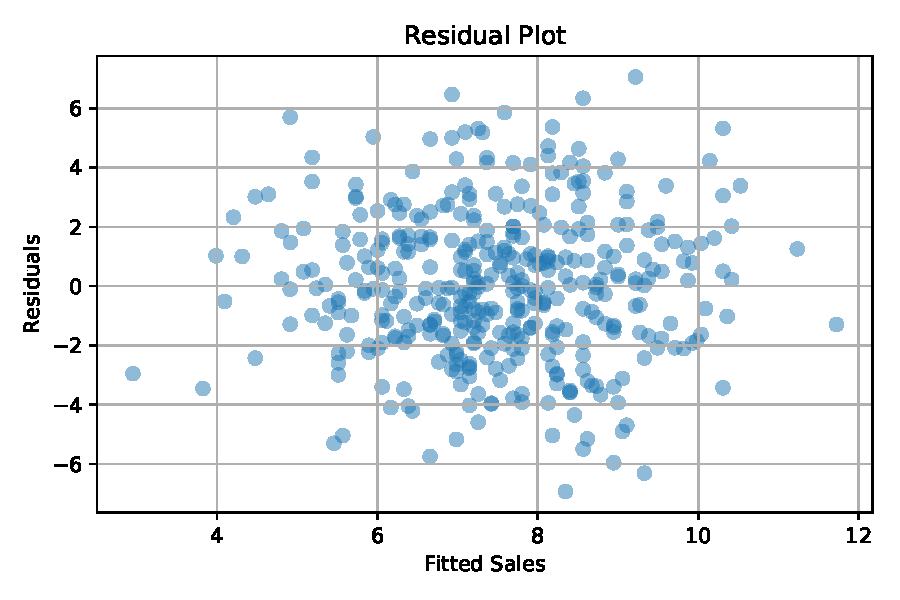
\includegraphics[width = 0.80\textwidth]{1-resplot.pdf}
    \caption{Residuales como función del valor ajustado}
    \label{fig:1-resplot}
\end{figure}
\begin{figure}[H]
    \centering
    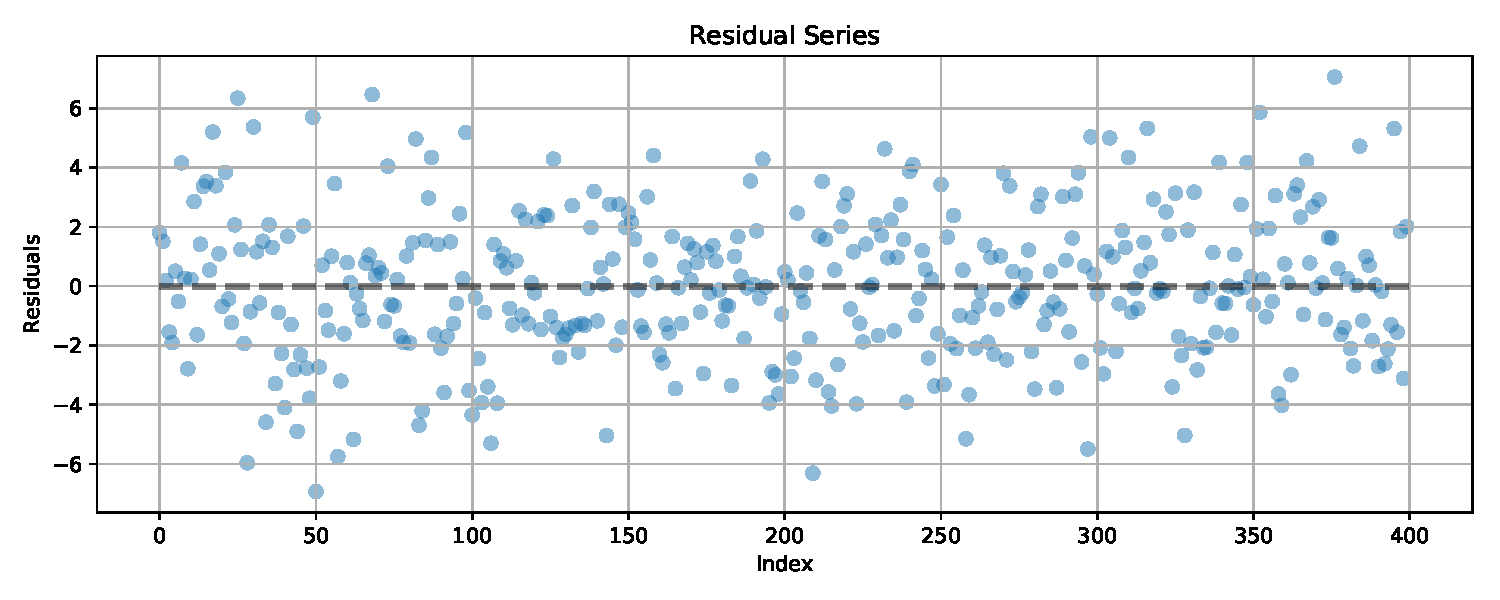
\includegraphics[width = 0.9\textwidth]{1-restimeplot.pdf}
    \caption{Residuales como función del índice}
    \label{fig:1-restimeplot}
\end{figure}
En principio, aunque hay una gran cantidad de puntos que tienen un residuo grande, no hay ninguo que destaque en particular por tener un residuo demasiado alejado de los otros. Pensando que este es uno de los mejores criterios para encontrar outliers, podemos concluir que en realidad no existen dichos puntos en nuestro conjunto de datos.
\\
\\Podemos ver más figuras del sistema para confirmar dicho hecho:
\begin{figure}[H]
    \centering
    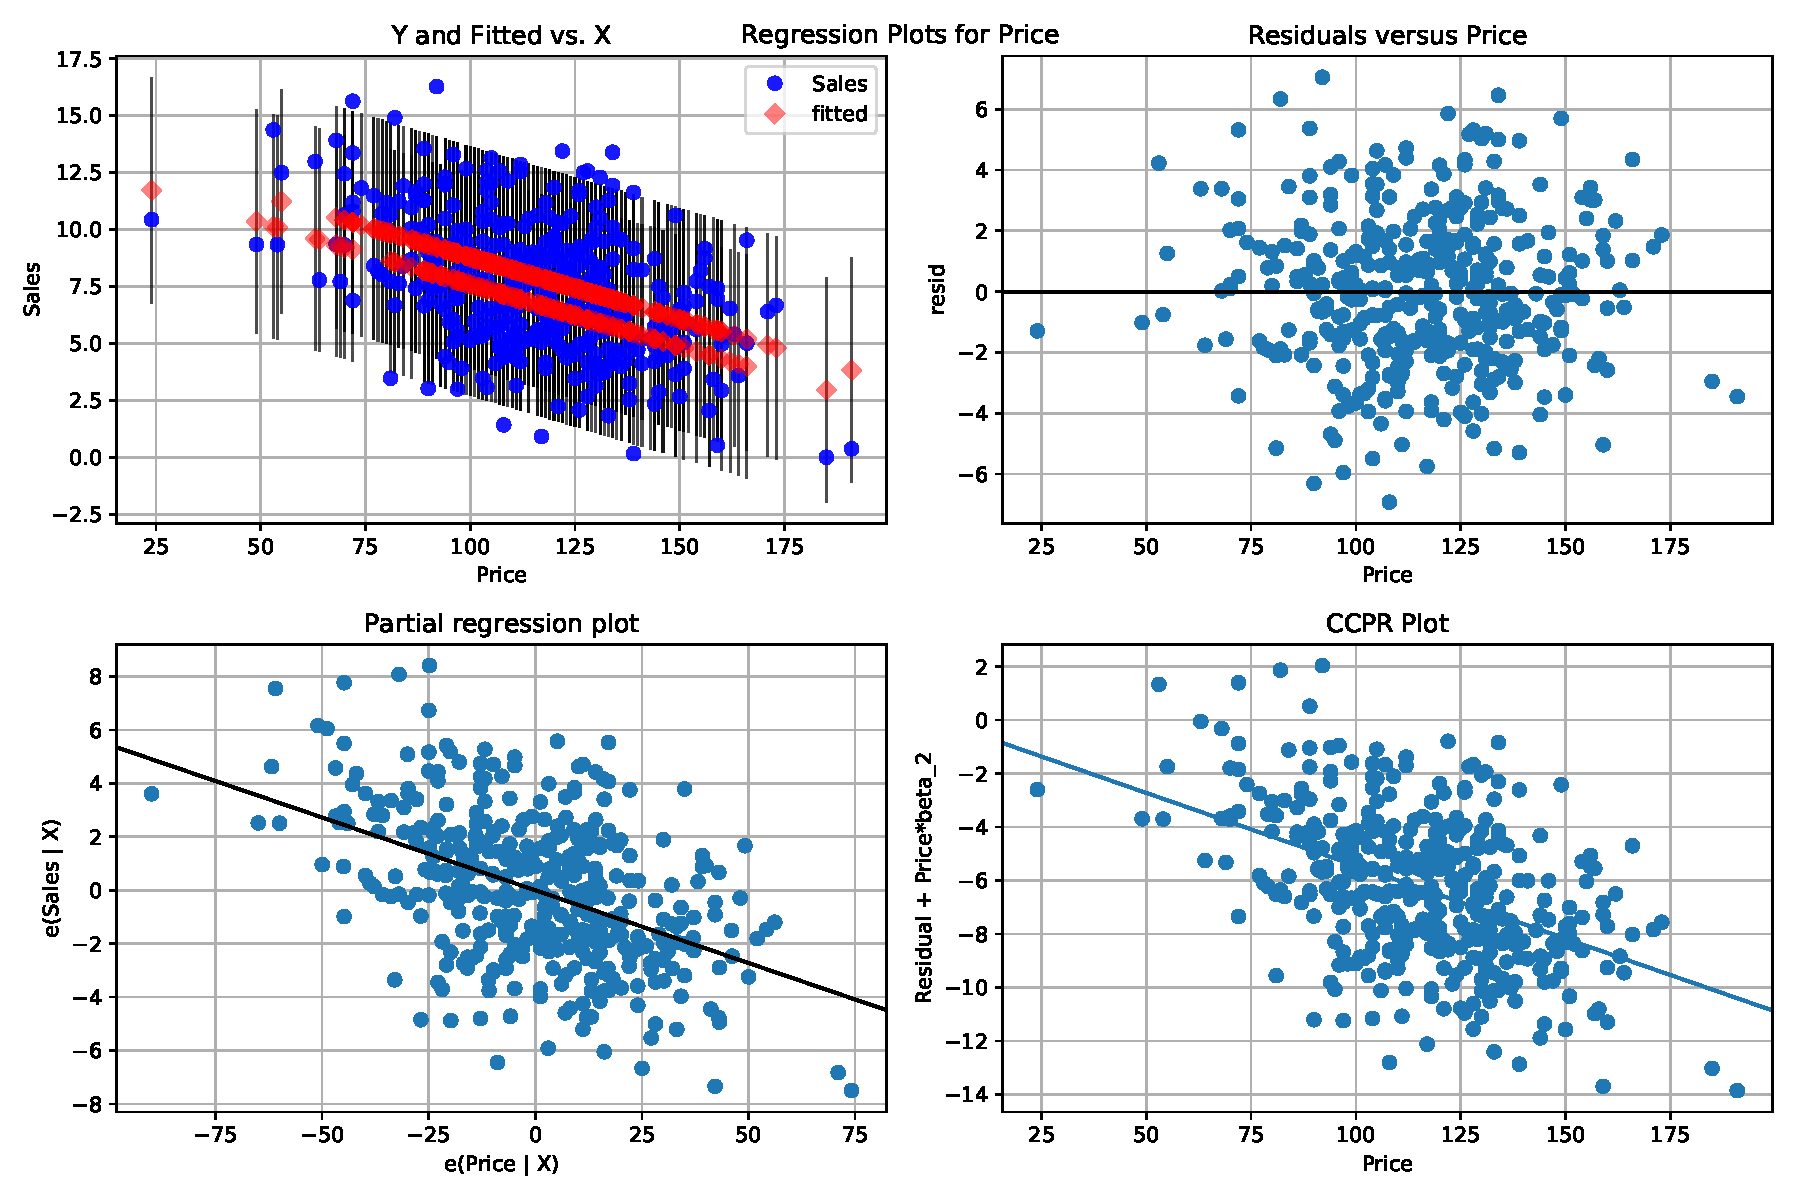
\includegraphics[width = 0.9\textwidth]{1-regdiag.pdf}
    \caption{Ajuste y CCPR}
    \label{fig:1-restimeplot}
\end{figure}
\begin{figure}[H]
    \centering
    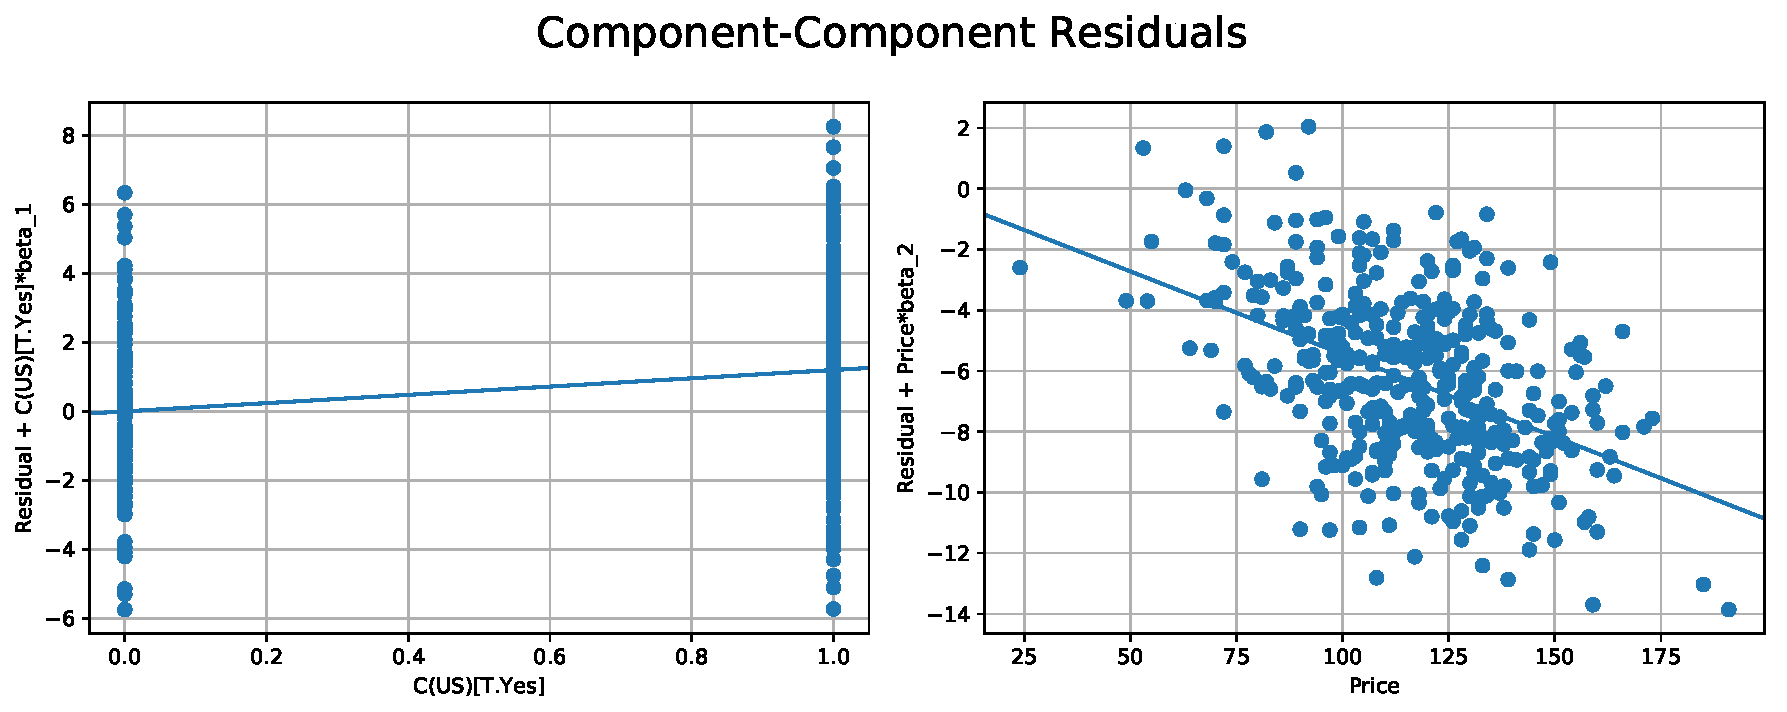
\includegraphics[width = 0.9\textwidth]{1-compcomp.pdf}
    \caption{Residuales para cada variable}
    \label{fig:1-compcomp}
\end{figure}
\begin{figure}[H]
    \centering
    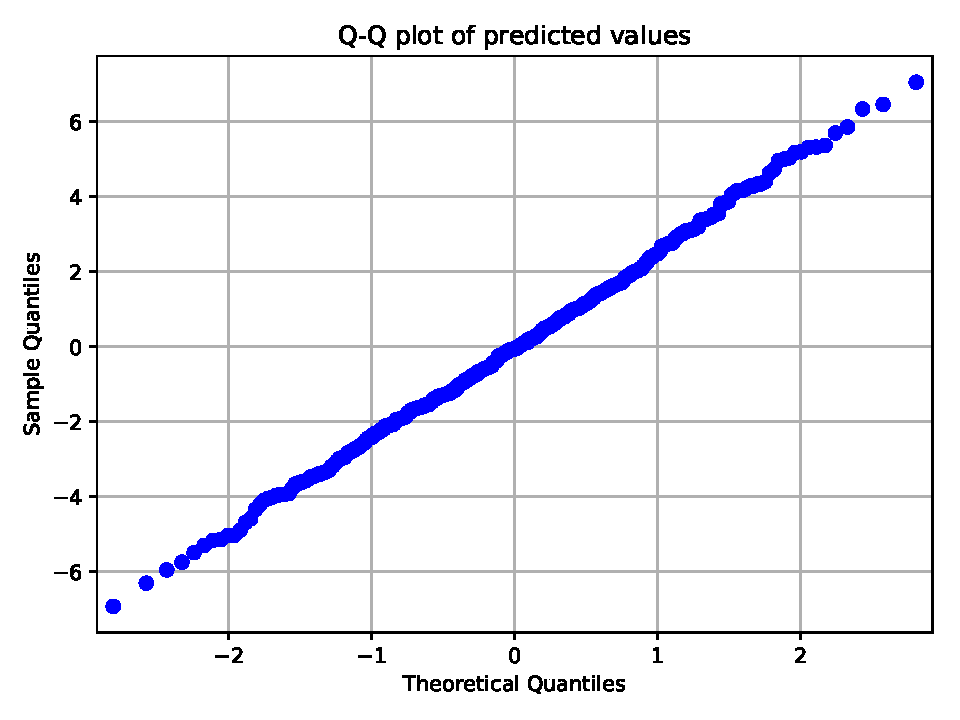
\includegraphics[width = 0.6\textwidth]{1-qqplot.pdf}
    \caption{qq-plot para los cuantiles de los residuales}
    \label{fig:1-qqplot}
\end{figure}
En ninguno de estos puntos detectamos outliers en nuestros datos. Por otro lado, para intentar verificar si existen puntos de alta influencia podemos ver la gráfica del coeficiente $H$ en la figura \ref{fig:1-influence}
\begin{figure}[H]
    \centering
    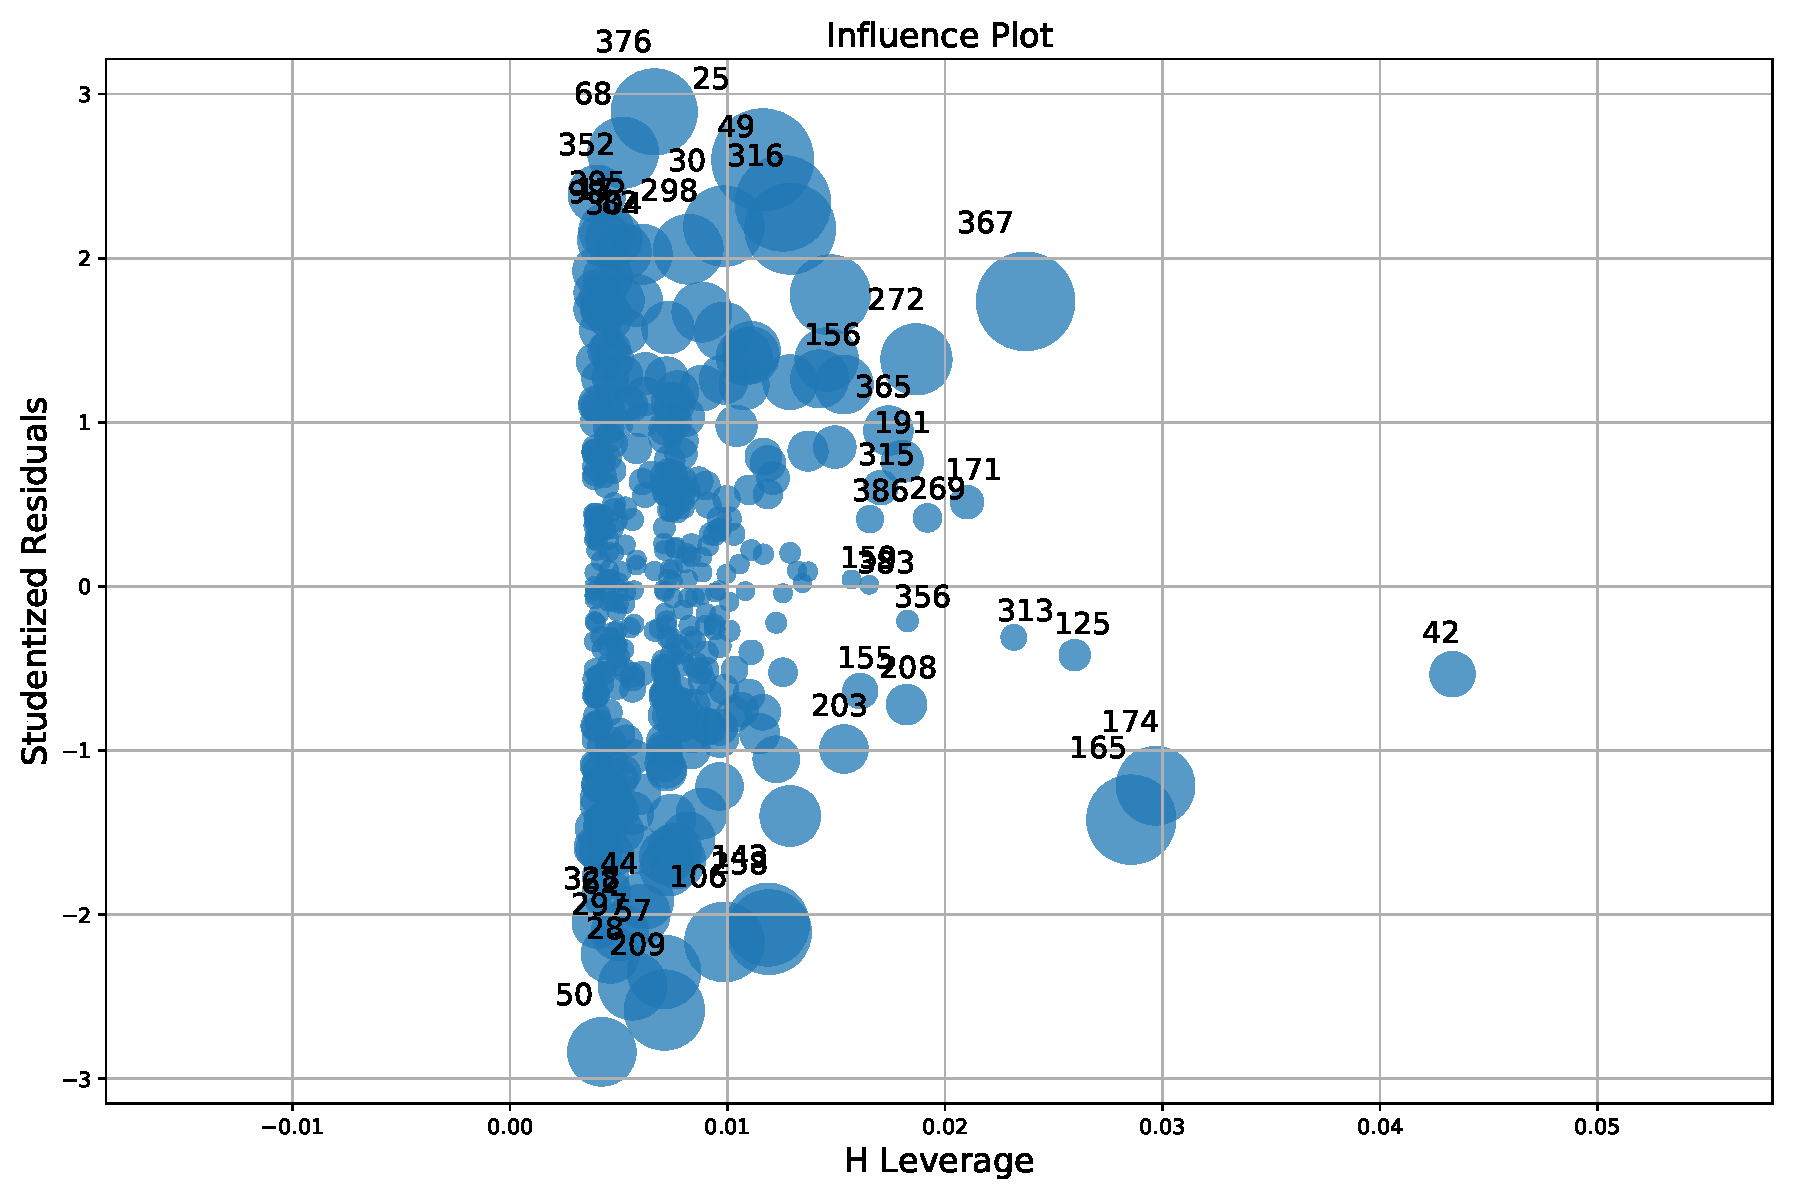
\includegraphics[width = 0.6\textwidth]{1-influence.pdf}
    \caption{qq-plot para los cuantiles de los residuales}
    \label{fig:1-influence}
\end{figure}
Pensando en la gráfica del coeficiente $H$, aunque tienen un valor pequeño, nos señala a los puntos de datos 42,174 y 165 como posibles puntos de alta influencia. Podemos ver explícitamente sus valores en la base de datos en la tabla \ref{tab:1-outliers}
\begin{table}[H]
    \begin{tabular}{lrrrrrrlrrll}
\toprule
{} &  Sales &  CompPrice &  Income &  Advertising &  Population &  Price & ShelveLoc &  Age &  Education & Urban &   US \\
\midrule
42  &  10.43 &         77 &      69 &            0 &          25 &     24 &    Medium &   50 &         18 &   Yes &   No \\
174 &   0.00 &        139 &      24 &            0 &         358 &    185 &    Medium &   79 &         15 &    No &   No \\
165 &   0.37 &        147 &      58 &            7 &         100 &    191 &       Bad &   27 &         15 &   Yes &  Yes \\
\bottomrule
\end{tabular}

    \caption{Posibles puntos de alta influencia}
    \label{tab:1-outliers}
\end{table}
Es claro que todos tiene un valor inusual de Price, pero no afirmaría que ninguno es de alta influencia debido a que  su coeficiente $H$ sigue siendo bastante pequeño relativo a los valores esperados para puntos de alto impacto ($H \geq 0.2$) \cite{isl}.
\section{Ejercicio 1: Problema 10, capítulo 3 \cite{isl}}
\subsection{Inciso a)}
Generamos los datos de manera aleatoria como indica el problema y como se muestra en el anexo 2 del reporte, para obtener los datos que muestra en la tabla \ref{tab:2-data}
\begin{table}[H]
    \centering
    \begin{tabular}{lrrr}
\toprule
{} &        x1 &        x2 &         y \\
\midrule
0 &  0.417022 &  0.240074 &  2.949735 \\
1 &  0.720324 &  0.157942 &  3.261717 \\
2 &  0.000114 & -0.030563 &  3.322517 \\
3 &  0.302333 &  0.233964 &  2.387546 \\
4 &  0.146756 &  0.096387 &  3.002498 \\
\bottomrule
\end{tabular}

    \caption{Posibles puntos de alta influencia}
    \label{tab:2-data}
\end{table}
Nosotros sabemos que los datos tienen la forma:
\begin{equation}
    \label{2-mod}
    \begin{split}
        y &= \beta_0 + \beta_1 \cdot x1 + \beta_2 \cdot x2 + \epsilon \\
         &= 2 + 2 \cdot x1 + 0.3 \cdot x2 + \epsilon \\
         &= 2 + 2 \cdot x1 + 0.3 \cdot 0.5 \cdot x1 + \epsilon \\
         &= 2 + 2.15 \cdot x1 + \epsilon \\
    \end{split}
\end{equation}
\subsection{Inciso b)}
La figura \ref{fig:2-corr} muestra un scatter plot entre x1 y x2 así como su correlación
\begin{figure}[H]
    \centering
    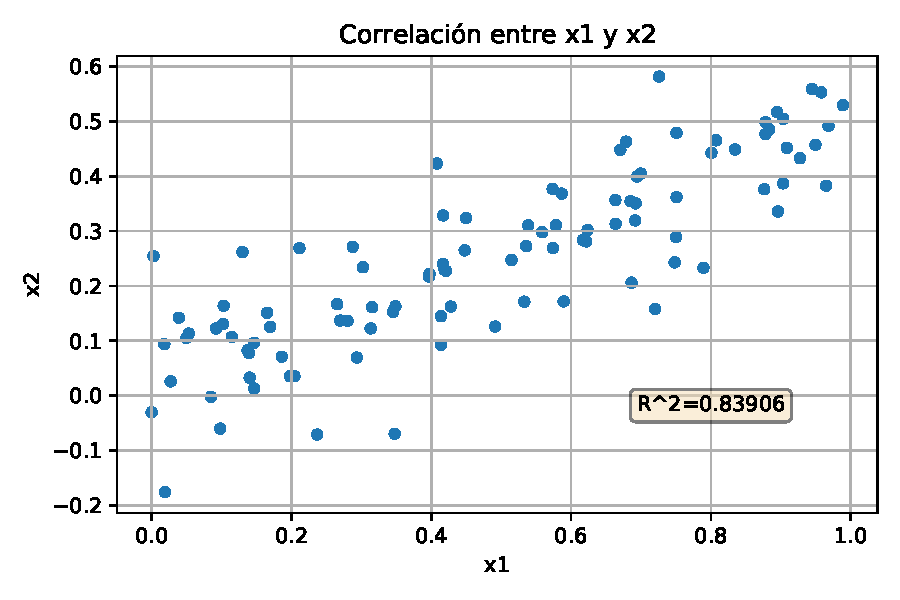
\includegraphics[width=0.6\textwidth]{2-corr.pdf}
    \caption{Correlación entre x1 y x2}
    \label{fig:2-corr}
\end{figure}
Aunque, debido a la escala, en la gráfica no se vea de manera muy clara, existe una alta correlación entre ambos puntos, Esto se asenta como un hecho cuando vemos que el valor de $R^2$ es sumamente alto. 
\subsection{Inciso c)}
Procedemos a realizar una regresión lineal tomando en cuenta ambas variables, para obtener los coeficientes de la tabla \ref{tab:2-mod1}
\begin{table}[H]
    \centering
    \begin{tabular}{lrrrrrr}
\toprule
{} &     Coef. &  Std.Err. &          t &   \$P (> |t|)\$ &    [0.025 &    0.975] \\
\midrule
Intercept &  2.189284 &  0.198655 &  11.020556 &  8.532403e-19 &  1.795010 &  2.583559 \\
x1        &  0.704629 &  0.636765 &   1.106575 &  2.712146e-01 & -0.559175 &  1.968432 \\
x2        &  2.502405 &  1.140433 &   2.194259 &  3.060418e-02 &  0.238962 &  4.765848 \\
\bottomrule
\end{tabular}

    \caption{Coeficientes para el modelo lineal de ambas variables}
    \label{tab:2-mod1}
\end{table}
El valor de los coeficientes obtenidos es sumamente distinto de la ecuación \ref{2-mod}. En particular, $\beta_1$ está muy lejos en valor porcentual del verdadero valor. Fijandonos en los p-values, podríamos aceptar la hipótesis de $\beta_1=0$ y quizá también la de $\beta_2 = 0$. Sin embargo,aunque no es suficientemente bajo, el p-value de $\beta_2$ esta un orden de magnitud abajo del de $\beta_1$, lo que complica la desición de aceptar $\beta_2 = 0$.
\subsection{Inciso d)}
Tomando en cuenta solo a x1, obtenemos los coeficientes de la tabla \ref{tab:2-mod2}
\begin{table}[H]
    \centering
    \begin{tabular}{lrrrrrr}
\toprule
{} &     Coef. &  Std.Err. &          t &   \$P (> |t|)\$ &    [0.025 &    0.975] \\
\midrule
Intercept &  2.248581 &  0.200602 &  11.209167 &  2.942644e-19 &  1.850493 &  2.646669 \\
x1        &  1.876987 &  0.353104 &   5.315681 &  6.683125e-07 &  1.176264 &  2.577709 \\
\bottomrule
\end{tabular}

    \caption{Coeficientes para el modelo lineal de x1}
    \label{tab:2-mod2}
\end{table}
Es claro que los p-values son sumamente bajos, lo que implica rechazar la hipótesis de que $\beta_1 = 0$.
\subsection{Inciso e)}
Por último, tomando en cuenta solo a x2, obtenemos los coeficientes de la tabla \ref{tab:2-mod3}
\begin{table}[H]
    \centering
    \begin{tabular}{lrrrrrr}
\toprule
{} &     Coef. &  Std.Err. &          t &   \$P (> |t|)\$ &    [0.025 &    0.975] \\
\midrule
Intercept &  2.265526 &  0.186537 &  12.145167 &  2.952030e-21 &  1.895349 &  2.635703 \\
x2        &  3.561276 &  0.621151 &   5.733353 &  1.090964e-07 &  2.328623 &  4.793930 \\
\bottomrule
\end{tabular}

    \caption{Coeficientes para el modelo lineal de x2}
    \label{tab:2-mod3}
\end{table}
Nuevamente nos inclinamos a rechazar $\beta_1 = 0$  debido al bajo p-value.
\subsection{Inciso f)}
Para comparar los tres modelos, podemos ver la tabla \ref{tab:2-modComp}
que compara las estadísticas imporantes de los tres modelos
\begin{table}[H]
    \centering
    \begin{tabular}{lrrrrrr}
\toprule
      Model &  R-squared &         AIC &         BIC &  Log-Likelihood &  F-statistic &  Prob (F-statistic) \\
\midrule
 y \textasciitilde  x1 +x2 &   0.260508 &  290.679208 &  298.494719 &     -142.339604 &    17.085577 &        4.398146e-07 \\
     y \textasciitilde  x1 &   0.223802 &  293.523632 &  298.733973 &     -144.761816 &    28.256462 &        6.683125e-07 \\
      y \textasciitilde x2 &   0.251173 &  289.933686 &  295.144026 &     -142.966843 &    32.871342 &        1.090964e-07 \\
\bottomrule
\end{tabular}

    \caption{Comparación de modelos}
    \label{2-modComp}
\end{table}
Notemos que ni el $R^2$ ni el logaritmo de la verosimilitud muestran una mejora sustancial entre los modelos, aunque cabe señalar que el de dos variables tiene el mayor valor. El valor de la estadística $F$ para los tres si tiene un valor distinto, pero la prueba $P(>F)$ no cambia sustancialmente, por lo que nuevamente no encontramos diferencia significativa entre los modelos
\\
La respuesta a la pregunta de si estos resultados de los tres incisos anteriores son consistentes entre sí, en principio, pareciera ser que no, que existe una inconsistencia entre ambos.
\\
\\Sin embargo, retomando el hecho de que los puntos son colineales y fueron generados añadiendo números aleatorios con distribución normal, se puede explicar que la alta correlación entre sus variables hace más inestable la regresión y hace difícil de comparar la aceptación u rechazo de hipótesis entre los tres casos.
\subsection{Inciso g)}
Si añadimos una observación $(x1,x2,y) = (0.1,0.8,0.6)$, podemos primero visualizar el valor en el plano $x1-x2$, mostrado en la figura \ref{fig:2-newData}, para entender si será un punto de alta influencia.
\begin{figure}[H]
    \centering
    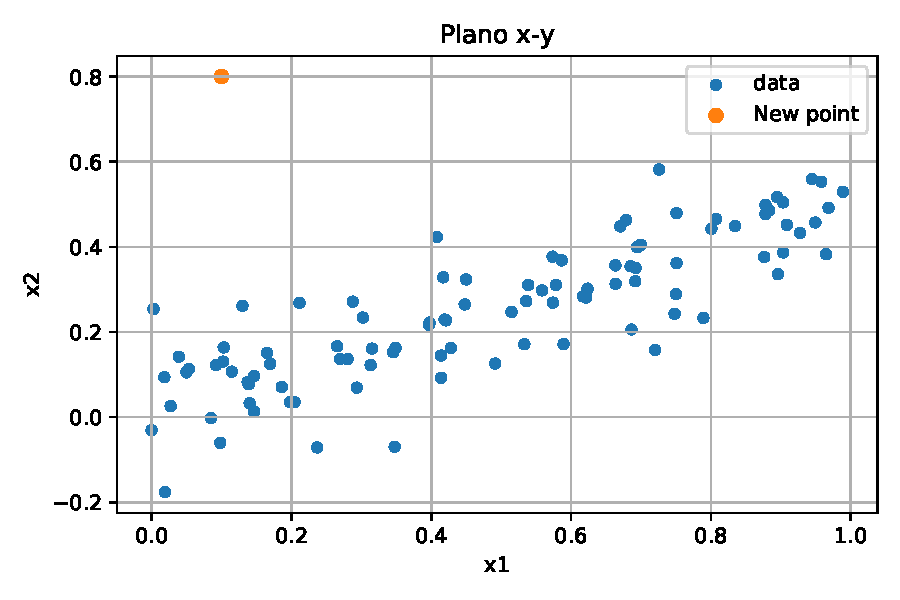
\includegraphics[width = 0.8\textwidth]{2-newData.pdf}
    \caption{Nueva observación}
    \label{fig:2-newData}
\end{figure}
Parece ser un dato muy alejado de los valores normales de las otras observaciones, por lo que podría considerarse de alta influencia. Para ver si también es un outlier, podemos realizar los mismos ajustes anteriores:
\begin{table}[H]
    \centering
    \begin{tabular}{lrrrrrr}
\toprule
{} &     Coef. &  Std.Err. &          t &   \$P (> |t|)\$ &    [0.025 &    0.975] \\
\midrule
Intercept &  2.167608 &  0.205090 &  10.569045 &  7.071833e-18 &  1.760613 &  2.574603 \\
x1        &  1.725411 &  0.535528 &   3.221884 &  1.729105e-03 &  0.662672 &  2.788149 \\
x2        &  0.529136 &  0.917938 &   0.576440 &  5.656396e-01 & -1.292483 &  2.350755 \\
\bottomrule
\end{tabular}

    \caption{Coeficientes para el nuevo modelo lineal de ambas variables}
    \label{tab:2-newMod1}
\end{table}
\begin{table}[H]
    \centering
    \begin{tabular}{lrrrrrr}
\toprule
{} &     Coef. &  Std.Err. &          t &   \$P (> |t|)\$ &    [0.025 &    0.975] \\
\midrule
Intercept &  2.192032 &  0.199988 &  10.960836 &  8.877601e-19 &  1.795213 &  2.588851 \\
x1        &  1.956577 &  0.353723 &   5.531375 &  2.595173e-07 &  1.254713 &  2.658441 \\
\bottomrule
\end{tabular}

    \caption{Coeficientes para el nuevo modelo lineal de x1}
    \label{tab:2-newMod2}
\end{table}
\begin{table}[H]
    \centering
    \begin{tabular}{lrrrrrr}
\toprule
{} &     Coef. &  Std.Err. &          t &   \$P (> |t|)\$ &    [0.025 &    0.975] \\
\midrule
Intercept &  2.430716 &  0.196842 &  12.348559 &  9.275744e-22 &  2.040139 &  2.821293 \\
x2        &  2.743821 &  0.636535 &   4.310557 &  3.849638e-05 &  1.480797 &  4.006845 \\
\bottomrule
\end{tabular}

    \caption{Coeficientes para el nuevo modelo lineal de x2}
    \label{tab:2-newMod3}
\end{table}
Analizamos ahora el residual estandarizado del nuevo punto en todos los modelos:
\begin{table}[H]
    \centering
    \begin{tabular}{lr}
        \hline
        Modelo & Residual estandarizado \\
        \hline
        $y \sim x1 +x2$ & -20.8429 \\
        $y \sim x1 $ & -17.1936 \\
        $y \sim x2$ & -36.8806 \\
        \hline
    \end{tabular}
    \caption{Residual estandarizado}
    \label{tab:2-newMod3}
\end{table}
El valor de su residual estandarizado es muy alto para todos los ajustes, cosa que nos indica también que el punto parece ser un outlier. De ambos valores, podemos concluir que el punto es tanto un outlier como un punto de alta influencia: sus valores tanto en $y$ como en $x1$,$x2$ son inusuales para los del conjunto de datos.
\\
\\En general, también observamos que $R^2$ y la estadística $F$ no mejoraron mucho para estos ajustes en comparación con los anteriores. La diferencia más interesante entre estos ajustes y los realizados anteriormente se encuentra en los p-values del ajuste de las dos variables, pues aquí ya no nos permite rechazar la hipótesis de que $\beta_1 = 0$ de manera tan sencilla.
\\
\\Los coeficientes del modelo de dos variables también mejoran, aunque no sustancialemente, para asemejarse al modelo original.
\section{Ejercicio 2}
Tenemos 23137 observaciones de 14 variables, de las cuales queremos usar 13, todas categóricas, para estimar 1 llamada ``Crash\_Score''. Los datos se pueden observar en la tabla \ref{tab:3-data}
\begin{table}[H]
    \centering
    \begin{tabular}{cccccp{2cm}p{2cm}p{2cm}p{2cm}p{2cm}p{2cm}p{2cm}p{2cm}p{2cm}p{2cm}}
\toprule
{} &  Crash\_Score &  year & Month & Time\_of\_Day & Rd\_Feature &    Rd\_Character &   Rd\_Class &          Rd\_Configuration &      Rd\_Surface & Rd\_Conditions &         Light & Weather & Traffic\_Control & Work\_Area \\
\midrule
0 &         6.56 &  2016 &     6 &           2 &       NONE &  STRAIGHT-LEVEL &  STATE HWY &  TWO-WAY-PROTECTED-MEDIAN &  SMOOTH ASPHALT &           DRY &      DAYLIGHT &   CLEAR &            NONE &        NO \\
1 &         6.53 &  2016 &     6 &           3 &       NONE &  STRAIGHT-LEVEL &      OTHER &         TWO-WAY-NO-MEDIAN &  COARSE ASPHALT &           DRY &      DAYLIGHT &   CLEAR &            NONE &        NO \\
2 &         1.58 &  2016 &     6 &           5 &       NONE &  STRAIGHT-LEVEL &  STATE HWY &         TWO-WAY-NO-MEDIAN &  SMOOTH ASPHALT &           DRY &  DARK-NOT-LIT &   CLEAR &            NONE &        NO \\
3 &         7.15 &  2016 &     6 &           3 &       NONE &  STRAIGHT-LEVEL &      OTHER &         TWO-WAY-NO-MEDIAN &  SMOOTH ASPHALT &           DRY &      DAYLIGHT &   CLEAR &            NONE &        NO \\
4 &         9.57 &  2016 &     6 &           6 &       NONE &  STRAIGHT-LEVEL &      OTHER &         TWO-WAY-NO-MEDIAN &  COARSE ASPHALT &           DRY &      DARK-LIT &   CLEAR &            NONE &        NO \\
\bottomrule
\end{tabular}

    \caption{Conjunto de datos}
    \label{tab:3-data}
\end{table}
Queremos encontrar un modelo lineal que ajuste de manera buena los datos. Antes de querer tomar un modelo arbitrario, al estar tratando con variables categóricas, debemos tomar alguna como referencia para cada categoría. 
\\
\\Ya que en principio las distribución del Crash\_Score puede cambiar entre categorías de la misma variable, realizamos boxplots e histogramas de el valor del Crash\_Score para cada categoría. A continuación mostramos dos gráficas para categorías distintas en las figuras\ref{fig:3-yearHist} y \ref{fig:3-WeatherHist}
\begin{figure}[H]
    \centering
    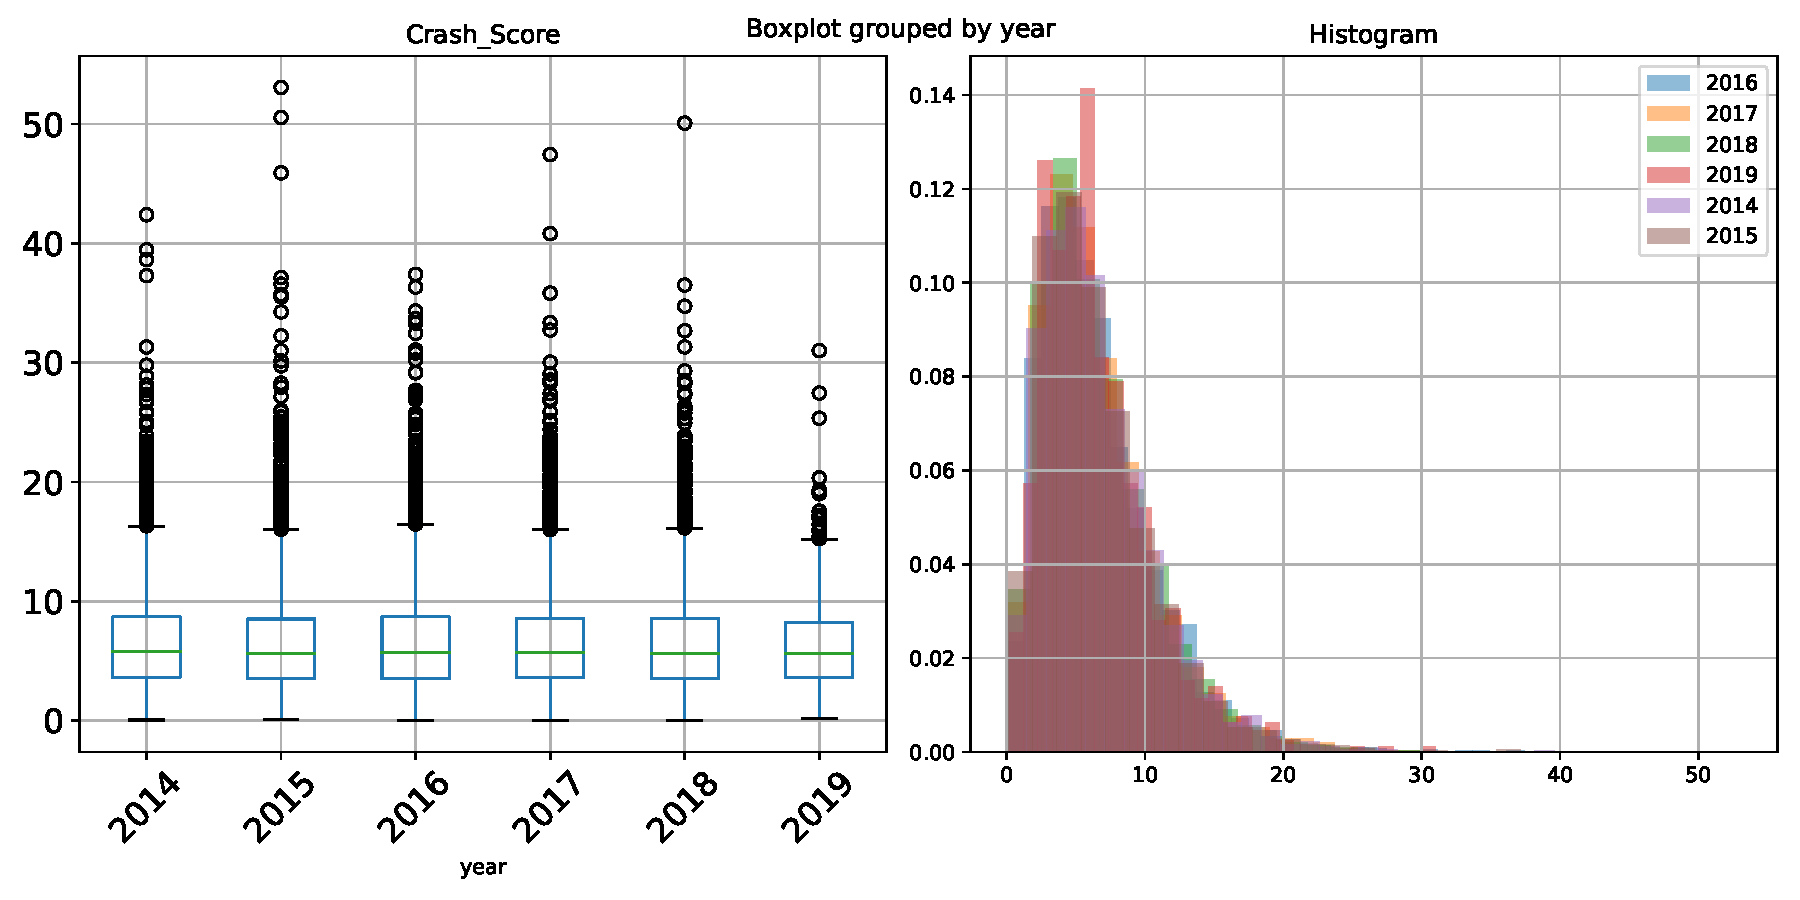
\includegraphics[width = 0.95\textwidth]{3-yearHist.pdf}
    \caption{Boxplot e histograma para variable year}
    \label{fig:3-yearHist}
\end{figure}
\begin{figure}[H]
    \centering
    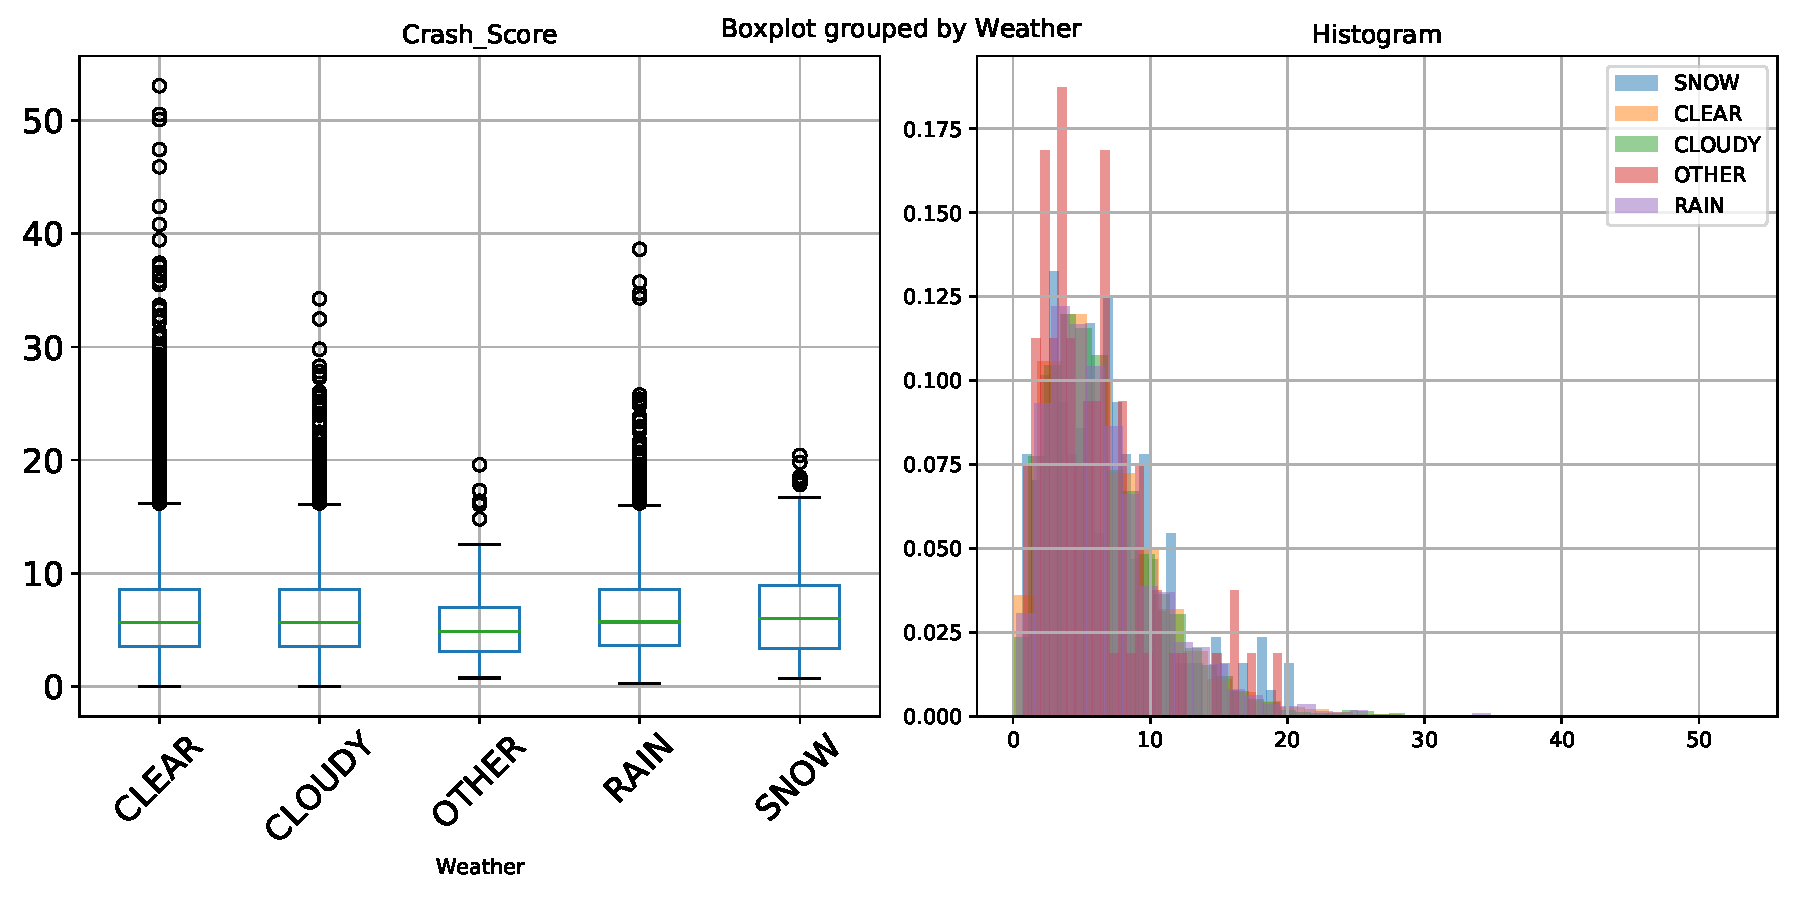
\includegraphics[width = 0.95\textwidth]{3-WeatherHist.pdf}
    \caption{Boxplot e histograma para variable Weather}
    \label{fig:3-WeatherHist}
\end{figure}
Antes que cualquier cosa, la forma del boxplot nos indica que la distribución de la variable no es simétrica. Esto provoca que el análisis inmediato de dichas gráficas no sea tan sencillo. En la figura \ref{fig:3-yearHist} se ve claramente que la distribución por año no tiene ninguna diferencia observable, mientras que en la figura \ref{fig:3-WeatherHist} la única distribución que destaca es la de la categoría ``OTHER'', lo cual se explica en el hecho de que ahí puede haber observaciones o bien mal catalogadas o difíciles de predecir.
\\
\\Para ver si existe alguna influencia del tiempo, podemos ver el valor del Crash\_Score como función del tiempo para una variable de tiempo en unidades arbitrarias definida como $(\text{year}-2014) \cdot 12 \cdot 6 + \text{Month} \cdot 6 + \text{Time\_of\_Day}$. La figura \ref{sig} muestra dicha gráfica.
\begin{figure}[H]
    \centering
    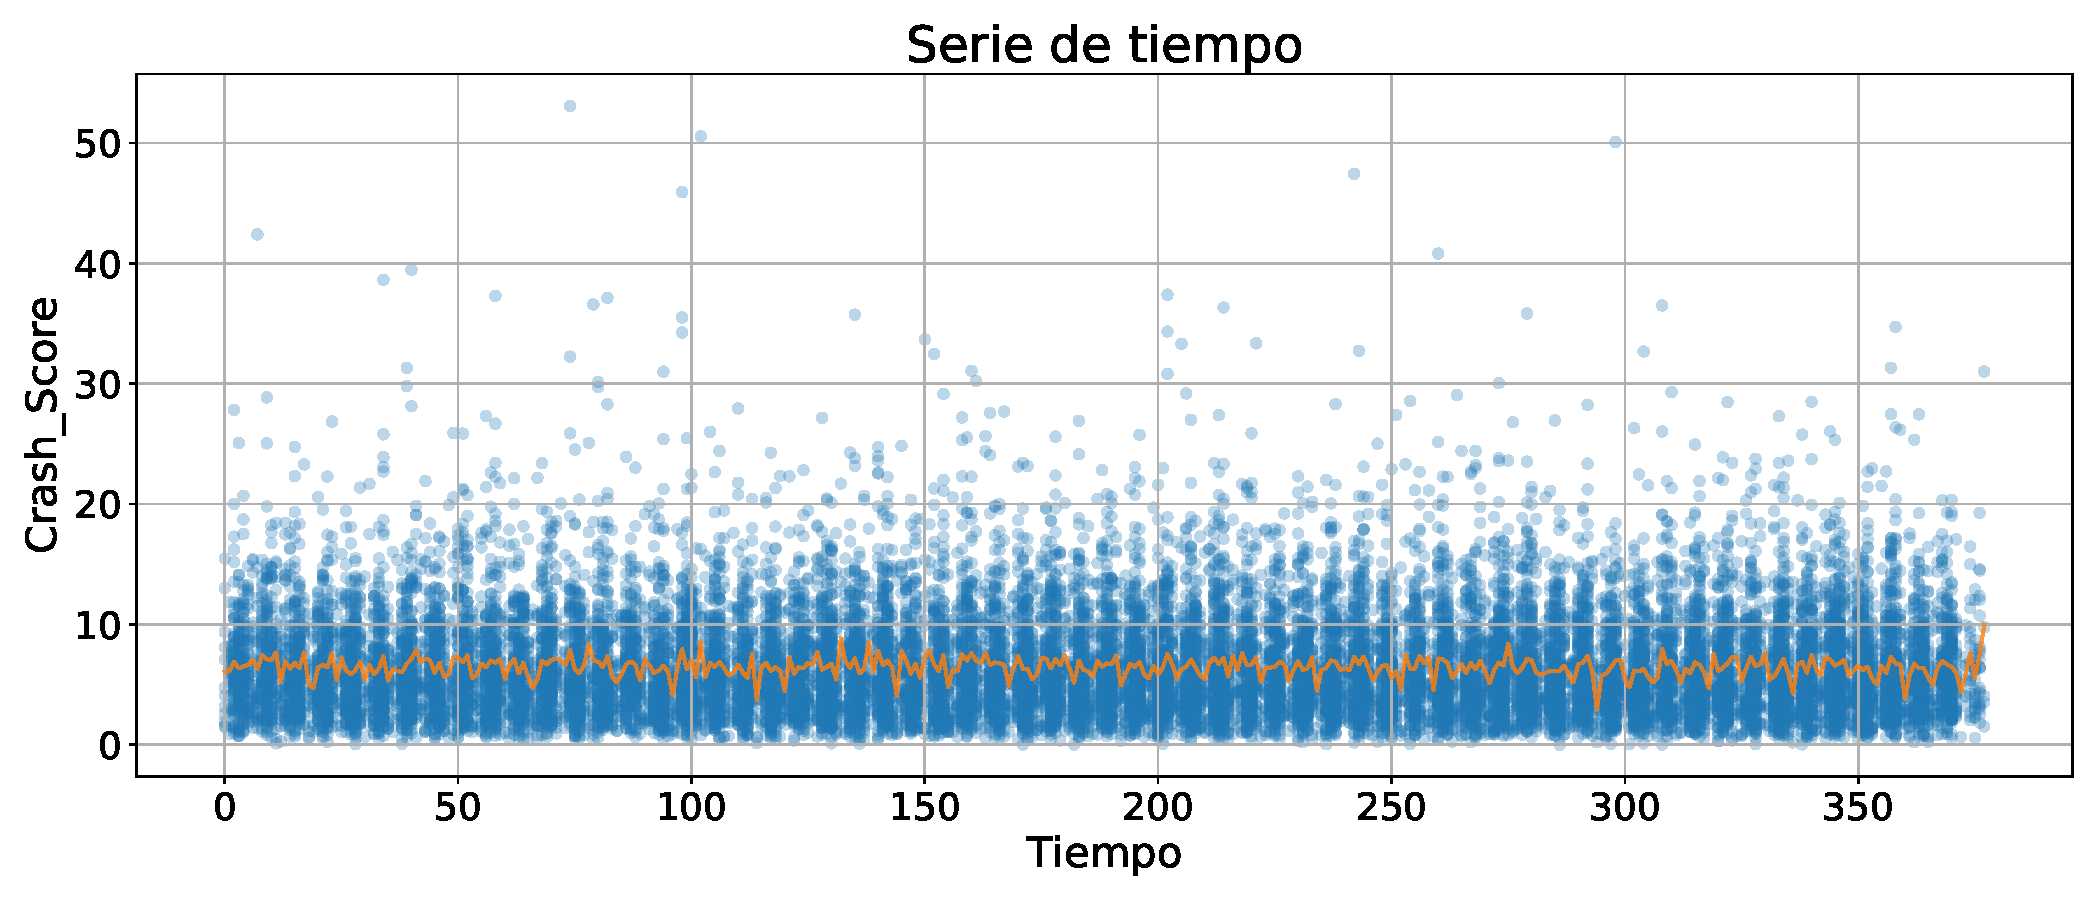
\includegraphics[width = 0.9\textwidth]{3-timeplot.pdf}
    \caption{Crash\_Score como función del tiempo}
    \label{sig}
\end{figure}
Es claro que no parece haber ninguna relación simple entre el tiempo y el valor del Crash\_Score. 
Así, dado que estas observaciones no permiten escoger objetivamente categorías de referencia, se tuvieron que escoger con justificaciones arbitrarias  o de sentido común. La tabla \ref{3-refers} muestra la categoría de referencia para todas las variables
\begin{table}[H]
    \centering
    \begin{tabular}{ccp{3cm}}    
             
     \hline
     Variable & Referencia & Justificación \\
     \hline
     year  & 2014  & Arbitrario \\
     & & \\
     Month  & 10  & Mes sin vacaciones escolares o personales  \\
     & & \\
     Time\_of\_Day  & 4  & Horario con hora de comida y no sobrecargado \\
     & & \\
     Rd\_Feature  & NONE  & Comparar con caminos normales \\
     & & \\
     Rd\_Character  & STRAIGHT-LEVEL  & Compara con caminos sin peralte o curvas \\
     & & \\
     Rd\_Class  & OTHER  & Arbitrario \\
     & & \\
     Rd\_Configuration  & TWO-WAY-UNPROTECTED-MEDIAN  & Camino más representativo \\
     & & \\
     Rd\_Surface  & SMOOTH ASPHALT  & Material más representativo \\
     & & \\
     Rd\_Conditions  & OTHER  & Arbitrario \\
     & & \\
     Light  & DAYLIGHT  & Luz más estándar \\
     & & \\
     Weather  & CLEAR  & Clima más estándar \\
     & & \\
     Traffic\_Control  & NONE  & Arbitrario \\
     & & \\
     Work\_Area & NO & Quitar influencia por tráfico \\
     & & \\
     \hline
    \end{tabular}
    \caption{Referencias para cada variable categórica}
    \label{tab:3-data}
\end{table}
Se ajustaron en total 7 modelos a los datos, cuyas ecuaciones mostramos a continuación
\begin{table}[H]
    \centering
    \begin{tabular}{c | p{15cm}}
        \hline
        Modelo & Ecuación \\
        \hline
        0 & Crash\_Score ~  + year + Month + Time\_of\_Day + Rd\_Feature   + Rd\_Character   + Rd\_Class   + Rd\_Configuration + Rd\_Surface  T + Rd\_Conditions   + Light   + Weather   + Traffic\_Control   + Work\_Area   \\
        1 & Crash\_Score\_boxcox\_0\_27 ~  + year + Month + Time\_of\_Day + Rd\_Feature   + Rd\_Character   + Rd\_Class   + Rd\_Configuration + Rd\_Surface  T + Rd\_Conditions   + Light   + Weather   + Traffic\_Control   + Work\_Area   \\
        2 & Crash\_Score\_boxcox\_0\_27 ~  + Time\_of\_Day + Rd\_Feature   + Rd\_Character   + Rd\_Class   + Rd\_Surface  T + Light   + Traffic\_Control   \\
        3 & Crash\_Score\_boxcox\_0\_27 ~  + Rd\_Class   + Traffic\_Control   + Time\_of\_Day*Light + Rd\_Feature*Rd\_Character*Rd\_Surface \\
        4 & Crash\_Score\_boxcox\_0\_27 ~  + Rd\_Class   + Traffic\_Control   + Rd\_Feature*Rd\_Character*Rd\_Surface*Time\_of\_Day + Rd\_Feature*Rd\_Character*Rd\_Surface*Light \\
        5 & Crash\_Score\_boxcox\_0\_27 ~ + Rd\_Class + Traffic\_Control + Rd\_Feature+ Rd\_Character+ Rd\_Surface+ Time\_of\_Day+ Light+ Rd\_Feature:Rd\_Character+ Rd\_Feature:Rd\_Surface+ Rd\_Feature:Time\_of\_Day+ Rd\_Character:Time\_of\_Day+ Rd\_Surface:Time\_of\_Day+ Rd\_Feature:Light+ Rd\_Character:Light+ Rd\_Feature:Rd\_Character:Rd\_Surface+ Rd\_Feature:Rd\_Surface:Time\_of\_Day+ Rd\_Feature:Rd\_Character:Light+ Rd\_Feature:Rd\_Character:Rd\_Surface:Light \\
        6 & Crash\_Score\_boxcox\_0\_27 ~ + Rd\_Class + Traffic\_Control + Rd\_Feature+ Rd\_Character+ Rd\_Surface+ Time\_of\_Day+ Light+ Rd\_Feature:Rd\_Character+ Rd\_Feature:Rd\_Surface+ Rd\_Surface:Time\_of\_Day+ Rd\_Character:Light+ Rd\_Feature:Rd\_Surface:Time\_of\_Day+ Rd\_Feature:Rd\_Character:Rd\_Surface:Light \\
        \hline
    \end{tabular}
    \caption{Ecuaciones de cada modelo}
    \label{3-comparison}
\end{table}
La variable ``Crash\_Score\_boxcox\_0\_27'' representa a ``Crash\_Score'' después de haber realizado un transformación Box-Cox con $\lambda = 0.27$. Se tomó ese valor de lambda pues ese era el que maximizaba el logaritmo de la verosimilitud, como se muestra en la figura \ref{fig:3-boxcox}
\begin{figure}[H]
    \centering
    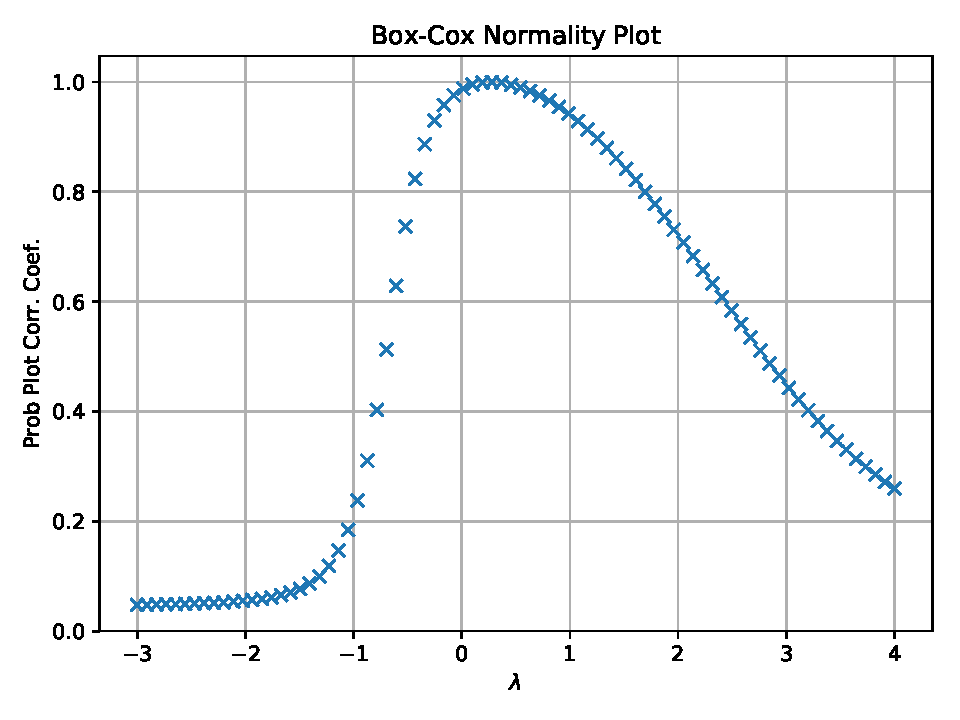
\includegraphics[width = 0.6\textwidth]{3-boxcox.pdf}
    \caption{verosimilitud como función de $\lambda$ para transformaciones boxcox de la variable Crash\_Score}
    \label{fig:3-boxcox}
\end{figure}
Empezamos en el modelo 0, un modelo lineal normal, y luego pasamos al modelo 1 haciendo la transformación boxcox. Para pasar al modelo 2, buscábamos reducir las variables.
\\
\\Para reducir variables, se utilizó también un script de R que, utilizando la función \text{step{stats}}, reducía las variables de modelo hasta obtener un conjunto más pequeño fijándose en el criterio AIC. Las variables que quedaron en el modelo fueron Time\_of\_Day, Rd\_Feature  , Rd\_Character  , Rd\_Class  , Rd\_Surface  T, Light  y Traffic\_Control. Este resultado también era consistente con el análisis ANOVA de las variables para el modelo 1. El modelo 2 trabajaba exactamente con estas variables de manera lineal.
\\
\\Los modelos 3-6 trabajan con las mismas variables pero realizando distintas interacciones. Las interacciones fueron definidas de manera arbitraria, aunque se buscó que interactuaran entre ellas variables que no tiene mucha relación en el plano semántico (Time\_of\_Day con las características del camino, por ejemplo)
\\
\\Para analizar a fondo la representabilidad de las variables de cada modelo, remitimos al lector al anexo 1 del presente trabajo donde se muestran las tablas ANOVA de cada modelo. No se pueden presentar las tablas de los p-values e intervalos de confianza de todas las variables ya que, al codificarse en variables dummies, el número de variables crece considerablemente y no es posible incluir esa información en el presente trabajo
\\
\\Finalmente, presentamos la siguiente tabla comparando todos los modelos realizados
\begin{table}[H]
    \centering
    \begin{tabular}{lrrrrrr}
\toprule
{} &  R-squared &            AIC &            BIC &  Log-Likelihood &  F-statistic &  Prob (F-statistic) \\
model &            &                &                &                 &              &                     \\
\midrule
0     &   0.017116 &  132646.376793 &  133121.278906 &   -66264.188397 &     6.929017 &        2.266000e-52 \\
1     &   0.019800 &   67662.540049 &   68137.442161 &   -33772.270024 &     8.037371 &        2.602486e-64 \\
2     &   0.018763 &   67630.995836 &   67880.520674 &   -33784.497918 &    14.727664 &        5.746884e-74 \\
3     &   0.026283 &   67707.006692 &   68978.778451 &   -33695.503346 &     3.950638 &        2.687955e-55 \\
4     &   0.048653 &   68165.253070 &   73445.520625 &   -33426.626535 &     1.755272 &        1.614963e-28 \\
5     &   0.040874 &   67983.678981 &   71774.846693 &   -33520.839491 &     2.055153 &        2.346331e-35 \\
6     &   0.039879 &   67953.659358 &   71527.498984 &   -33532.829679 &     2.127681 &        4.934881e-37 \\
\bottomrule
\end{tabular}

    \caption{Comparación de modelos}
    \label{3-comparison}
\end{table}
Fijándo la atención en el parámetro $R^2$, es claro que el modelo 4 presenta el valor más grande de este parámetro. Para $P(> F)$, dicho modelo no presenta el mejor valor. En cuanto al logaritmo de la verosimilitud, es claro que el modelo 4 también presenta el máximo valor de todos los otros modelos. Revisando su qqplot en la figura \ref{qqplotok}, confirmamos su adecuación.
\begin{figure}[H]
    \centering
    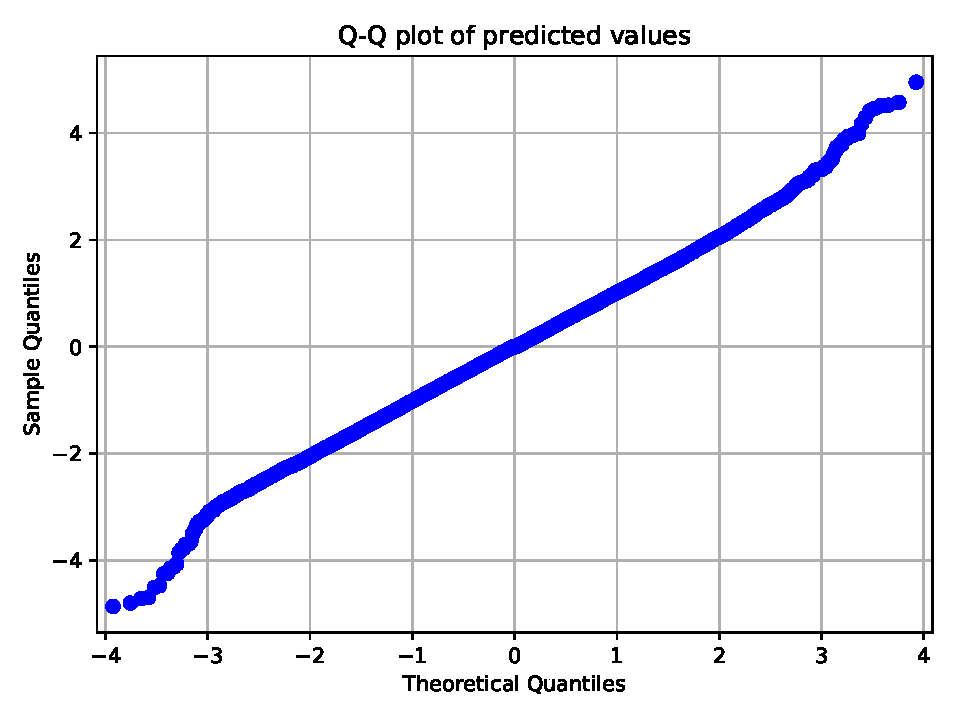
\includegraphics[width = 0.7\textwidth]{3-qqplot4.pdf}
    \caption{Q-Q Plot de los residuales del modelo 4}
    \label{qqplotok}
\end{figure}
Así, podemos concluir que el modelo 4 presenta el mejor ajuste y, tomando en cuenta el valor $R^2$, es el que presenta mayor estabilidad para predicción. Lo distintivo del model es que toma en cuenta las interacciones de la luz del día y la hora con las características del camino. Podemos interpretar que estas interacciones son las más significativas a la hora de predecir cuando puede darse un accidente de tráfico: cuando las características climáticas y la visibilidad, representadas por la luz del día, al igual que el tráfico, representado por la hora, interactúan con las características del camino.
\pagebreak
\section*{Anexo 1: Tablas Anova y de Coeficientes de los modelos del ejercicio 2}
\subsection*{Modelo 0}
\begin{longtable}{p{6cm}lccccc}
\toprule
{} &         df &      sum\_sq &   mean\_sq &       F &  \$P (> F\$) \\
Variable         &            &             &           &         &            \\
\midrule
\endhead
\midrule
\multicolumn{6}{r}{{Continued on next page}} \\
\midrule
\endfoot

\bottomrule
\endlastfoot
year             &     5.0000 &     61.5800 &   12.3160 &  0.6827 &     0.6366 \\
Month            &    11.0000 &    101.7591 &    9.2508 &  0.5128 &     0.8962 \\
Time\_of\_Day      &     5.0000 &    751.2592 &  150.2518 &  8.3282 &     0.0000 \\
Rd\_Feature       &     4.0000 &   2485.7422 &  621.4356 & 34.4453 &     0.0000 \\
Rd\_Character     &     6.0000 &    292.0400 &   48.6733 &  2.6979 &     0.0128 \\
Rd\_Class         &     2.0000 &   2045.5863 & 1022.7931 & 56.6919 &     0.0000 \\
Rd\_Configuration &     4.0000 &     17.1126 &    4.2781 &  0.2371 &     0.9175 \\
Rd\_Surface       &     4.0000 &    188.2856 &   47.0714 &  2.6091 &     0.0337 \\
Rd\_Conditions    &     3.0000 &     20.4264 &    6.8088 &  0.3774 &     0.7693 \\
Light            &     5.0000 &    661.0898 &  132.2180 &  7.3286 &     0.0000 \\
Weather          &     4.0000 &    119.5621 &   29.8905 &  1.6568 &     0.1570 \\
Traffic\_Control  &     4.0000 &    400.3357 &  100.0839 &  5.5475 &     0.0002 \\
Work\_Area        &     1.0000 &    105.6916 &  105.6916 &  5.8583 &     0.0155 \\
Residual         & 23078.0000 & 416355.9220 &   18.0412 &     NaN &        NaN \\
\end{longtable}

\begin{table}[H]
    \centering
    \caption{ANOVA para modelo 0}
    \label{3-mod0Anova}
\end{table}
\subsection*{Modelo 1}
\begin{longtable}{p{6cm}lccccc}
\toprule
{} &         df &     sum\_sq &  mean\_sq &       F &  \$P (> F\$) \\
Variable         &            &            &          &         &            \\
\midrule
\endhead
\midrule
\multicolumn{6}{r}{{Continued on next page}} \\
\midrule
\endfoot

\bottomrule
\endlastfoot
year             &     5.0000 &     2.6001 &   0.5200 &  0.4781 &     0.7929 \\
Month            &    11.0000 &     4.5389 &   0.4126 &  0.3794 &     0.9646 \\
Time\_of\_Day      &     5.0000 &    69.2948 &  13.8590 & 12.7423 &     0.0000 \\
Rd\_Feature       &     4.0000 &   165.8339 &  41.4585 & 38.1180 &     0.0000 \\
Rd\_Character     &     6.0000 &    30.6552 &   5.1092 &  4.6975 &     0.0001 \\
Rd\_Class         &     2.0000 &   111.0778 &  55.5389 & 51.0639 &     0.0000 \\
Rd\_Configuration &     4.0000 &     0.9758 &   0.2439 &  0.2243 &     0.9250 \\
Rd\_Surface       &     4.0000 &    15.9737 &   3.9934 &  3.6717 &     0.0054 \\
Rd\_Conditions    &     3.0000 &     1.4278 &   0.4759 &  0.4376 &     0.7261 \\
Light            &     5.0000 &    55.8626 &  11.1725 & 10.2723 &     0.0000 \\
Weather          &     4.0000 &     8.6196 &   2.1549 &  1.9813 &     0.0944 \\
Traffic\_Control  &     4.0000 &    38.0889 &   9.5222 &  8.7550 &     0.0000 \\
Work\_Area        &     1.0000 &     2.0712 &   2.0712 &  1.9043 &     0.1676 \\
Residual         & 23078.0000 & 25100.4577 &   1.0876 &     NaN &        NaN \\
\end{longtable}

\begin{table}[H]
    \centering
    \caption{ANOVA para modelo 1}
    \label{3-mod1Anova}
\end{table}
\subsection*{Modelo 2}
\begin{longtable}{p{6cm}lccccc}
\toprule
{} &         df &     sum\_sq &  mean\_sq &       F &  \$P (> F\$) \\
Variable        &            &            &          &         &            \\
\midrule
\endhead
\midrule
\multicolumn{6}{r}{{Continued on next page}} \\
\midrule
\endfoot

\bottomrule
\endlastfoot
Time\_of\_Day     &     5.0000 &    68.4482 &  13.6896 & 12.5886 &     0.0000 \\
Rd\_Feature      &     4.0000 &   166.2881 &  41.5720 & 38.2283 &     0.0000 \\
Rd\_Character    &     6.0000 &    30.1610 &   5.0268 &  4.6225 &     0.0001 \\
Rd\_Class        &     2.0000 &   111.2879 &  55.6439 & 51.1684 &     0.0000 \\
Rd\_Surface      &     4.0000 &    15.0100 &   3.7525 &  3.4507 &     0.0080 \\
Light           &     5.0000 &    51.9180 &  10.3836 &  9.5484 &     0.0000 \\
Traffic\_Control &     4.0000 &    37.3621 &   9.3405 &  8.5893 &     0.0000 \\
Residual        & 23106.0000 & 25127.0029 &   1.0875 &     NaN &        NaN \\
\end{longtable}

\begin{table}[H]
    \centering
    \caption{ANOVA para modelo 2}
    \label{3-mod2Anova}
\end{table}
\subsection*{Modelo 3}
\begin{longtable}{p{6cm}lccccc}
\toprule
{} &         df &     sum\_sq &  mean\_sq &       F &  \$P (> F\$) \\
Variable                                  &            &            &          &         &            \\
\midrule
\endhead
\midrule
\multicolumn{6}{r}{{Continued on next page}} \\
\midrule
\endfoot

\bottomrule
\endlastfoot
Rd\_Class                                  &     2.0000 &   174.9344 &  87.4672 & 80.6077 &     0.0000 \\
Traffic\_Control                           &     4.0000 &   112.3334 &  28.0833 & 25.8809 &     0.0000 \\
Time\_of\_Day                               &     5.0000 &    65.1064 &  13.0213 & 12.0001 &     0.0000 \\
Light                                     &     5.0000 &    51.4740 &  10.2948 &  9.4874 &     0.0000 \\
Rd\_Feature                                &     4.0000 &    39.8064 &   9.9516 &  9.1712 &     0.0000 \\
Rd\_Character                              &     6.0000 &    23.6664 &   3.9444 &  3.6351 &     0.0013 \\
Rd\_Surface                                &     4.0000 &    13.1543 &   3.2886 &  3.0307 &     0.0165 \\
 : Time\_of\_Day : Light                    &    25.0000 &    41.8994 &   1.6760 &  1.5445 &     0.0404 \\
 : Rd\_Feature : Rd\_Character              &    24.0000 &    39.1408 &   1.6309 &  1.5030 &     0.0542 \\
 : Rd\_Feature : Rd\_Surface                &    16.0000 &    30.5494 &   1.9093 &  1.7596 &     0.0304 \\
 : Rd\_Character : Rd\_Surface              &    24.0000 &    18.2593 &   0.7608 &  0.7011 &     0.8559 \\
 : Rd\_Feature : Rd\_Character : Rd\_Surface &    96.0000 &   120.3806 &   1.2540 &  1.1556 &     0.1419 \\
Residual                                  & 22979.0000 & 24934.4466 &   1.0851 &     NaN &        NaN \\
\end{longtable}

\begin{table}[H]
    \centering
    \caption{ANOVA para modelo 3}
    \label{3-mod3Anova}
\end{table}
\subsection*{Modelo 4}
\begin{longtable}{p{6cm}lccccc}
\toprule
{} &         df &     sum\_sq &  mean\_sq &       F &  \$P (> F\$) \\
Variable                                           &            &            &          &         &            \\
\midrule
\endhead
\midrule
\multicolumn{6}{r}{{Continued on next page}} \\
\midrule
\endfoot

\bottomrule
\endlastfoot
Rd\_Class                                           &     2.0000 &   174.9344 &  87.4672 & 80.7151 &     0.0000 \\
Traffic\_Control                                    &     4.0000 &   112.3334 &  28.0833 & 25.9154 &     0.0000 \\
Rd\_Feature                                         &     4.0000 &    40.4497 &  10.1124 &  9.3318 &     0.0000 \\
Rd\_Character                                       &     6.0000 &    29.5477 &   4.9246 &  4.5445 &     0.0001 \\
Rd\_Surface                                         &     4.0000 &    13.3979 &   3.3495 &  3.0909 &     0.0149 \\
Time\_of\_Day                                        &     5.0000 &    61.2545 &  12.2509 & 11.3052 &     0.0000 \\
Light                                              &     5.0000 &    48.5578 &   9.7116 &  8.9619 &     0.0000 \\
 : Rd\_Feature : Rd\_Character                       &    24.0000 &    39.9091 &   1.6629 &  1.5345 &     0.0456 \\
 : Rd\_Feature : Rd\_Surface                         &    16.0000 &    26.0955 &   1.6310 &  1.5051 &     0.0879 \\
 : Rd\_Character : Rd\_Surface                       &    24.0000 &    22.6416 &   0.9434 &  0.8706 &     0.6450 \\
 : Rd\_Feature : Time\_of\_Day                        &    20.0000 &    27.7317 &   1.3866 &  1.2795 &     0.1799 \\
 : Rd\_Character : Time\_of\_Day                      &    30.0000 &    38.7420 &   1.2914 &  1.1917 &     0.2165 \\
 : Rd\_Surface : Time\_of\_Day                        &    20.0000 &    30.8236 &   1.5412 &  1.4222 &     0.0994 \\
 : Rd\_Feature : Light                              &    20.0000 &    30.3820 &   1.5191 &  1.4018 &     0.1087 \\
 : Rd\_Character : Light                            &    30.0000 &    50.4859 &   1.6829 &  1.5530 &     0.0274 \\
 : Rd\_Surface : Light                              &    20.0000 &    18.9922 &   0.9496 &  0.8763 &     0.6186 \\
 : Rd\_Feature : Rd\_Character : Rd\_Surface          &    96.0000 &   106.9679 &   1.1142 &  1.0282 &     0.4047 \\
 : Rd\_Feature : Rd\_Character : Time\_of\_Day         &   120.0000 &   127.7655 &   1.0647 &  0.9825 &     0.5371 \\
 : Rd\_Feature : Rd\_Surface : Time\_of\_Day           &    80.0000 &   111.8225 &   1.3978 &  1.2899 &     0.0419 \\
 : Rd\_Character : Rd\_Surface : Time\_of\_Day         &   120.0000 &   120.3298 &   1.0027 &  0.9253 &     0.7085 \\
 : Rd\_Feature : Rd\_Character : Light               &   120.0000 &   135.3034 &   1.1275 &  1.0405 &     0.3627 \\
 : Rd\_Feature : Rd\_Surface : Light                 &    80.0000 &    82.2389 &   1.0280 &  0.9486 &     0.6093 \\
 : Rd\_Character : Rd\_Surface : Light               &   120.0000 &   124.2919 &   1.0358 &  0.9558 &     0.6193 \\
 : Rd\_Feature : Rd\_Character : Rd\_Surface : Tim... &   480.0000 &   484.3093 &   1.0090 &  0.9311 &     0.8557 \\
 : Rd\_Feature : Rd\_Character : Rd\_Surface : Light  &   480.0000 &   594.1913 &   1.2379 &  1.1423 &     0.0177 \\
Residual                                           & 22481.0000 & 24361.5993 &   1.0837 &     NaN &        NaN \\
\end{longtable}

\begin{table}[H]
    \centering
    \caption{ANOVA para modelo 4}
    \label{3-mod4Anova}
\end{table}
\subsection*{Modelo 5}
\begin{longtable}{p{6cm}lccccc}
\toprule
{} &         df &     sum\_sq &  mean\_sq &       F &  \$P (> F\$) \\
Variable                                          &            &            &          &         &            \\
\midrule
\endhead
\midrule
\multicolumn{6}{r}{{Continued on next page}} \\
\midrule
\endfoot

\bottomrule
\endlastfoot
Rd\_Class                                          &     2.0000 &   174.9344 &  87.4672 & 80.7193 &     0.0000 \\
Traffic\_Control                                   &     4.0000 &   112.3334 &  28.0833 & 25.9168 &     0.0000 \\
Rd\_Feature                                        &     4.0000 &    40.4497 &  10.1124 &  9.3323 &     0.0000 \\
Rd\_Character                                      &     6.0000 &    29.5477 &   4.9246 &  4.5447 &     0.0001 \\
Rd\_Surface                                        &     4.0000 &    13.3979 &   3.3495 &  3.0911 &     0.0149 \\
Time\_of\_Day                                       &     5.0000 &    61.2545 &  12.2509 & 11.3058 &     0.0000 \\
Light                                             &     5.0000 &    48.5578 &   9.7116 &  8.9623 &     0.0000 \\
 : Rd\_Feature : Rd\_Character                      &    24.0000 &    39.9091 &   1.6629 &  1.5346 &     0.0456 \\
 : Rd\_Feature : Rd\_Surface                        &    16.0000 &    26.0955 &   1.6310 &  1.5051 &     0.0878 \\
 : Rd\_Feature : Time\_of\_Day                       &    20.0000 &    27.0867 &   1.3543 &  1.2499 &     0.2017 \\
 : Rd\_Character : Time\_of\_Day                     &    30.0000 &    27.9352 &   0.9312 &  0.8593 &     0.6862 \\
 : Rd\_Surface : Time\_of\_Day                       &    20.0000 &    33.3872 &   1.6694 &  1.5406 &     0.0578 \\
 : Rd\_Feature : Light                             &    20.0000 &    29.9218 &   1.4961 &  1.3807 &     0.1190 \\
 : Rd\_Character : Light                           &    30.0000 &    47.6300 &   1.5877 &  1.4652 &     0.0483 \\
 : Rd\_Feature : Rd\_Character : Rd\_Surface         &   120.0000 &   131.8752 &   1.0990 &  1.0142 &     0.4397 \\
 : Rd\_Feature : Rd\_Surface : Time\_of\_Day          &    80.0000 &   112.4661 &   1.4058 &  1.2974 &     0.0385 \\
 : Rd\_Feature : Rd\_Character : Light              &   120.0000 &   134.2030 &   1.1184 &  1.0321 &     0.3867 \\
 : Rd\_Feature : Rd\_Character : Rd\_Surface : Light &   700.0000 &   681.6559 &   0.9738 &  0.8987 &     0.9725 \\
Residual                                          & 22666.0000 & 24560.8083 &   1.0836 &     NaN &        NaN \\
\end{longtable}

\begin{table}[H]
    \centering
    \caption{ANOVA para modelo 5}
    \label{3-mod5Anova}
\end{table}
\subsection*{Modelo 6}
\begin{longtable}{p{6cm}lccccc}
\toprule
{} &         df &     sum\_sq &  mean\_sq &       F &  \$P (> F\$) \\
Variable                                          &            &            &          &         &            \\
\midrule
\endhead
\midrule
\multicolumn{6}{r}{{Continued on next page}} \\
\midrule
\endfoot

\bottomrule
\endlastfoot
Rd\_Class                                          &     2.0000 &   174.9344 &  87.4672 & 80.7317 &     0.0000 \\
Traffic\_Control                                   &     4.0000 &   112.3334 &  28.0833 & 25.9208 &     0.0000 \\
Rd\_Feature                                        &     4.0000 &    40.4497 &  10.1124 &  9.3337 &     0.0000 \\
Rd\_Character                                      &     6.0000 &    29.5477 &   4.9246 &  4.5454 &     0.0001 \\
Rd\_Surface                                        &     4.0000 &    13.3979 &   3.3495 &  3.0916 &     0.0148 \\
Time\_of\_Day                                       &     5.0000 &    61.2545 &  12.2509 & 11.3075 &     0.0000 \\
Light                                             &     5.0000 &    48.5578 &   9.7116 &  8.9637 &     0.0000 \\
 : Rd\_Feature : Rd\_Character                      &    24.0000 &    39.9091 &   1.6629 &  1.5348 &     0.0456 \\
 : Rd\_Feature : Rd\_Surface                        &    16.0000 &    26.0955 &   1.6310 &  1.5054 &     0.0878 \\
 : Rd\_Surface : Time\_of\_Day                       &    20.0000 &    32.7552 &   1.6378 &  1.5116 &     0.0663 \\
 : Rd\_Character : Light                           &    30.0000 &    44.8885 &   1.4963 &  1.3811 &     0.0802 \\
 : Rd\_Feature : Rd\_Surface : Time\_of\_Day          &   100.0000 &   139.8376 &   1.3984 &  1.2907 &     0.0271 \\
 : Rd\_Feature : Rd\_Character : Rd\_Surface : Light &   960.0000 &  1056.2630 &   1.1003 &  1.0155 &     0.3646 \\
Residual                                          & 22693.0000 & 24586.2776 &   1.0834 &     NaN &        NaN \\
\end{longtable}

\begin{table}[H]
    \centering
    \caption{ANOVA para modelo 6}
    \label{3-mod6Anova}
\end{table}
%\begin{longtable}{p{6cm}lccccc}
\toprule
{} &         df &     sum\_sq &  mean\_sq &       F &  \$P (> F\$) \\
Variable                                          &            &            &          &         &            \\
\midrule
\endhead
\midrule
\multicolumn{6}{r}{{Continued on next page}} \\
\midrule
\endfoot

\bottomrule
\endlastfoot
Rd\_Class                                          &     2.0000 &   174.9344 &  87.4672 & 80.7193 &     0.0000 \\
Traffic\_Control                                   &     4.0000 &   112.3334 &  28.0833 & 25.9168 &     0.0000 \\
Rd\_Feature                                        &     4.0000 &    40.4497 &  10.1124 &  9.3323 &     0.0000 \\
Rd\_Character                                      &     6.0000 &    29.5477 &   4.9246 &  4.5447 &     0.0001 \\
Rd\_Surface                                        &     4.0000 &    13.3979 &   3.3495 &  3.0911 &     0.0149 \\
Time\_of\_Day                                       &     5.0000 &    61.2545 &  12.2509 & 11.3058 &     0.0000 \\
Light                                             &     5.0000 &    48.5578 &   9.7116 &  8.9623 &     0.0000 \\
 : Rd\_Feature : Rd\_Character                      &    24.0000 &    39.9091 &   1.6629 &  1.5346 &     0.0456 \\
 : Rd\_Feature : Rd\_Surface                        &    16.0000 &    26.0955 &   1.6310 &  1.5051 &     0.0878 \\
 : Rd\_Feature : Time\_of\_Day                       &    20.0000 &    27.0867 &   1.3543 &  1.2499 &     0.2017 \\
 : Rd\_Character : Time\_of\_Day                     &    30.0000 &    27.9352 &   0.9312 &  0.8593 &     0.6862 \\
 : Rd\_Surface : Time\_of\_Day                       &    20.0000 &    33.3872 &   1.6694 &  1.5406 &     0.0578 \\
 : Rd\_Feature : Light                             &    20.0000 &    29.9218 &   1.4961 &  1.3807 &     0.1190 \\
 : Rd\_Character : Light                           &    30.0000 &    47.6300 &   1.5877 &  1.4652 &     0.0483 \\
 : Rd\_Feature : Rd\_Character : Rd\_Surface         &   120.0000 &   131.8752 &   1.0990 &  1.0142 &     0.4397 \\
 : Rd\_Feature : Rd\_Surface : Time\_of\_Day          &    80.0000 &   112.4661 &   1.4058 &  1.2974 &     0.0385 \\
 : Rd\_Feature : Rd\_Character : Light              &   120.0000 &   134.2030 &   1.1184 &  1.0321 &     0.3867 \\
 : Rd\_Feature : Rd\_Character : Rd\_Surface : Light &   700.0000 &   681.6559 &   0.9738 &  0.8987 &     0.9725 \\
Residual                                          & 22666.0000 & 24560.8083 &   1.0836 &     NaN &        NaN \\
\end{longtable}

%\begin{table}[H]
%    \centering
%    \begin{longtable}{p{4cm}cccccc}
\toprule
{} &   Coef. &  Std.Err. &       t &  \$P (> |t|)\$ &  [0.025 &  0.975] \\
\midrule
\endhead
\midrule
\multicolumn{7}{r}{{Continued on next page}} \\
\midrule
\endfoot

\bottomrule
\endlastfoot
Intercept                                     &  6.8284 &    0.4378 & 15.5981 &       0.0000 &  5.9704 &  7.6865 \\
year [T.2015]                                 & -0.0933 &    0.0935 & -0.9978 &       0.3184 & -0.2765 &  0.0900 \\
year [T.2016]                                 & -0.0001 &    0.0926 & -0.0015 &       0.9988 & -0.1816 &  0.1813 \\
year [T.2017]                                 & -0.0556 &    0.0932 & -0.5961 &       0.5511 & -0.2383 &  0.1271 \\
year [T.2018]                                 & -0.1225 &    0.0920 & -1.3313 &       0.1831 & -0.3028 &  0.0578 \\
year [T.2019]                                 & -0.3337 &    0.1797 & -1.8568 &       0.0634 & -0.6860 &  0.0186 \\
Month [T.1]                                   &  0.0353 &    0.1354 &  0.2610 &       0.7941 & -0.2300 &  0.3007 \\
Month [T.2]                                   &  0.1068 &    0.1374 &  0.7772 &       0.4370 & -0.1625 &  0.3762 \\
Month [T.3]                                   & -0.0821 &    0.1339 & -0.6130 &       0.5399 & -0.3446 &  0.1804 \\
Month [T.4]                                   & -0.0447 &    0.1375 & -0.3251 &       0.7451 & -0.3143 &  0.2249 \\
Month [T.5]                                   & -0.1088 &    0.1317 & -0.8262 &       0.4087 & -0.3669 &  0.1493 \\
Month [T.6]                                   & -0.1196 &    0.1344 & -0.8893 &       0.3738 & -0.3831 &  0.1440 \\
Month [T.7]                                   & -0.1343 &    0.1385 & -0.9698 &       0.3322 & -0.4059 &  0.1372 \\
Month [T.8]                                   & -0.1143 &    0.1331 & -0.8588 &       0.3905 & -0.3753 &  0.1466 \\
Month [T.9]                                   & -0.1052 &    0.1347 & -0.7807 &       0.4350 & -0.3693 &  0.1589 \\
Month [T.11]                                  & -0.0907 &    0.1327 & -0.6832 &       0.4945 & -0.3509 &  0.1695 \\
Month [T.12]                                  &  0.0787 &    0.1318 &  0.5975 &       0.5502 & -0.1795 &  0.3370 \\
Time\_of\_Day [T.1]                             & -0.2942 &    0.1737 & -1.6936 &       0.0904 & -0.6346 &  0.0463 \\
Time\_of\_Day [T.2]                             & -0.1696 &    0.1212 & -1.4000 &       0.1615 & -0.4071 &  0.0679 \\
Time\_of\_Day [T.3]                             &  0.0392 &    0.0800 &  0.4897 &       0.6243 & -0.1176 &  0.1960 \\
Time\_of\_Day [T.5]                             &  0.2156 &    0.0767 &  2.8116 &       0.0049 &  0.0653 &  0.3659 \\
Time\_of\_Day [T.6]                             &  0.0940 &    0.1205 &  0.7802 &       0.4353 & -0.1421 &  0.3301 \\
Rd\_Feature [T.DRIVEWAY]                       &  0.1691 &    0.1004 &  1.6843 &       0.0921 & -0.0277 &  0.3658 \\
Rd\_Feature [T.INTERSECTION]                   &  0.3272 &    0.0841 &  3.8929 &       0.0001 &  0.1625 &  0.4920 \\
Rd\_Feature [T.OTHER]                          & -0.0807 &    0.2733 & -0.2952 &       0.7679 & -0.6165 &  0.4551 \\
Rd\_Feature [T.RAMP]                           & -0.5797 &    0.1998 & -2.9014 &       0.0037 & -0.9713 & -0.1881 \\
Rd\_Character [T.CURVE-GRADE]                  & -0.4181 &    0.1803 & -2.3195 &       0.0204 & -0.7715 & -0.0648 \\
Rd\_Character [T.CURVE-LEVEL]                  & -0.2827 &    0.1636 & -1.7278 &       0.0840 & -0.6035 &  0.0380 \\
Rd\_Character [T.CURVE-OTHER]                  &  0.2619 &    0.2852 &  0.9185 &       0.3584 & -0.2970 &  0.8209 \\
Rd\_Character [T.OTHER]                        & -0.4619 &    1.2011 & -0.3846 &       0.7005 & -2.8162 &  1.8924 \\
Rd\_Character [T.STRAIGHT-GRADE]               & -0.0114 &    0.0896 & -0.1271 &       0.8989 & -0.1870 &  0.1642 \\
Rd\_Character [T.STRAIGHT-OTHER]               & -0.3911 &    0.1673 & -2.3380 &       0.0194 & -0.7189 & -0.0632 \\
Rd\_Class [T.STATE HWY]                        &  0.5717 &    0.0730 &  7.8300 &       0.0000 &  0.4286 &  0.7148 \\
Rd\_Class [T.US HWY]                           &  0.8417 &    0.1307 &  6.4404 &       0.0000 &  0.5855 &  1.0978 \\
Rd\_Configuration [T.ONE-WAY]                  &  0.0106 &    0.1377 &  0.0771 &       0.9386 & -0.2593 &  0.2805 \\
Rd\_Configuration [T.TWO-WAY-NO-MEDIAN]        &  0.0439 &    0.0738 &  0.5955 &       0.5515 & -0.1007 &  0.1886 \\
Rd\_Configuration [T.TWO-WAY-PROTECTED-MEDIAN] &  0.1172 &    0.1124 &  1.0424 &       0.2972 & -0.1032 &  0.3375 \\
Rd\_Configuration [T.UNKNOWN]                  &  0.2399 &    0.5764 &  0.4162 &       0.6773 & -0.8899 &  1.3696 \\
Rd\_Surface [T.COARSE ASPHALT]                 &  0.1718 &    0.1007 &  1.7059 &       0.0880 & -0.0256 &  0.3692 \\
Rd\_Surface [T.CONCRETE]                       & -0.4120 &    0.1710 & -2.4097 &       0.0160 & -0.7472 & -0.0769 \\
Rd\_Surface [T.GROOVED CONCRETE]               & -0.0831 &    0.2416 & -0.3438 &       0.7310 & -0.5567 &  0.3906 \\
Rd\_Surface [T.OTHER]                          & -0.3394 &    0.5258 & -0.6454 &       0.5187 & -1.3699 &  0.6912 \\
Rd\_Conditions [T.DRY]                         & -0.7097 &    0.4151 & -1.7097 &       0.0873 & -1.5233 &  0.1039 \\
Rd\_Conditions [T.ICE-SNOW-SLUSH]              & -0.6453 &    0.5056 & -1.2763 &       0.2019 & -1.6362 &  0.3457 \\
Rd\_Conditions [T.WET]                         & -0.8967 &    0.4281 & -2.0945 &       0.0362 & -1.7358 & -0.0575 \\
Light [T.DARK-LIT]                            & -0.4560 &    0.1018 & -4.4807 &       0.0000 & -0.6555 & -0.2565 \\
Light [T.DARK-NOT-LIT]                        & -0.6566 &    0.1761 & -3.7288 &       0.0002 & -1.0017 & -0.3114 \\
Light [T.DAWN]                                & -0.2597 &    0.3677 & -0.7062 &       0.4801 & -0.9804 &  0.4611 \\
Light [T.DUSK]                                & -0.1182 &    0.1812 & -0.6521 &       0.5143 & -0.4733 &  0.2370 \\
Light [T.OTHER]                               & -0.9747 &    0.3186 & -3.0589 &       0.0022 & -1.5993 & -0.3501 \\
Weather [T.CLOUDY]                            & -0.0330 &    0.0899 & -0.3677 &       0.7131 & -0.2092 &  0.1431 \\
Weather [T.OTHER]                             & -0.8007 &    0.4928 & -1.6247 &       0.1042 & -1.7667 &  0.1653 \\
Weather [T.RAIN]                              &  0.2398 &    0.1645 &  1.4575 &       0.1450 & -0.0827 &  0.5623 \\
Weather [T.SNOW]                              &  0.1610 &    0.3868 &  0.4161 &       0.6773 & -0.5973 &  0.9192 \\
Traffic\_Control [T.OTHER]                     &  0.2292 &    0.2890 &  0.7931 &       0.4277 & -0.3372 &  0.7956 \\
Traffic\_Control [T.SIGNAL]                    &  0.3400 &    0.0881 &  3.8597 &       0.0001 &  0.1673 &  0.5127 \\
Traffic\_Control [T.STOP-SIGN]                 &  0.4422 &    0.1077 &  4.1046 &       0.0000 &  0.2310 &  0.6534 \\
Traffic\_Control [T.YIELD]                     &  0.2900 &    0.2822 &  1.0277 &       0.3041 & -0.2631 &  0.8432 \\
Work\_Area [T.YES]                             &  0.5882 &    0.2430 &  2.4204 &       0.0155 &  0.1119 &  1.0646 \\
\end{longtable}

%    \caption{Coeficientes para modelo 0}
%    \label{3-mod0Cof}
%\end{table}
%\begin{table}[H]
%    \centering
%    \begin{longtable}{p{6cm}lccccc}
\toprule
{} &         df &      sum\_sq &   mean\_sq &       F &  \$P (> F\$) \\
Variable         &            &             &           &         &            \\
\midrule
\endhead
\midrule
\multicolumn{6}{r}{{Continued on next page}} \\
\midrule
\endfoot

\bottomrule
\endlastfoot
year             &     5.0000 &     61.5800 &   12.3160 &  0.6827 &     0.6366 \\
Month            &    11.0000 &    101.7591 &    9.2508 &  0.5128 &     0.8962 \\
Time\_of\_Day      &     5.0000 &    751.2592 &  150.2518 &  8.3282 &     0.0000 \\
Rd\_Feature       &     4.0000 &   2485.7422 &  621.4356 & 34.4453 &     0.0000 \\
Rd\_Character     &     6.0000 &    292.0400 &   48.6733 &  2.6979 &     0.0128 \\
Rd\_Class         &     2.0000 &   2045.5863 & 1022.7931 & 56.6919 &     0.0000 \\
Rd\_Configuration &     4.0000 &     17.1126 &    4.2781 &  0.2371 &     0.9175 \\
Rd\_Surface       &     4.0000 &    188.2856 &   47.0714 &  2.6091 &     0.0337 \\
Rd\_Conditions    &     3.0000 &     20.4264 &    6.8088 &  0.3774 &     0.7693 \\
Light            &     5.0000 &    661.0898 &  132.2180 &  7.3286 &     0.0000 \\
Weather          &     4.0000 &    119.5621 &   29.8905 &  1.6568 &     0.1570 \\
Traffic\_Control  &     4.0000 &    400.3357 &  100.0839 &  5.5475 &     0.0002 \\
Work\_Area        &     1.0000 &    105.6916 &  105.6916 &  5.8583 &     0.0155 \\
Residual         & 23078.0000 & 416355.9220 &   18.0412 &     NaN &        NaN \\
\end{longtable}

%    \caption{ANOVA para modelo 0}
%    \label{3-mod0Anova}
%\end{table}
\begin{comment}
    \subsection*{Modelo 0}
\begin{table}[H]
    \centering
    \begin{longtable}{p{4cm}cccccc}
\toprule
{} &   Coef. &  Std.Err. &       t &  \$P (> |t|)\$ &  [0.025 &  0.975] \\
\midrule
\endhead
\midrule
\multicolumn{7}{r}{{Continued on next page}} \\
\midrule
\endfoot

\bottomrule
\endlastfoot
Intercept                                     &  6.8284 &    0.4378 & 15.5981 &       0.0000 &  5.9704 &  7.6865 \\
year [T.2015]                                 & -0.0933 &    0.0935 & -0.9978 &       0.3184 & -0.2765 &  0.0900 \\
year [T.2016]                                 & -0.0001 &    0.0926 & -0.0015 &       0.9988 & -0.1816 &  0.1813 \\
year [T.2017]                                 & -0.0556 &    0.0932 & -0.5961 &       0.5511 & -0.2383 &  0.1271 \\
year [T.2018]                                 & -0.1225 &    0.0920 & -1.3313 &       0.1831 & -0.3028 &  0.0578 \\
year [T.2019]                                 & -0.3337 &    0.1797 & -1.8568 &       0.0634 & -0.6860 &  0.0186 \\
Month [T.1]                                   &  0.0353 &    0.1354 &  0.2610 &       0.7941 & -0.2300 &  0.3007 \\
Month [T.2]                                   &  0.1068 &    0.1374 &  0.7772 &       0.4370 & -0.1625 &  0.3762 \\
Month [T.3]                                   & -0.0821 &    0.1339 & -0.6130 &       0.5399 & -0.3446 &  0.1804 \\
Month [T.4]                                   & -0.0447 &    0.1375 & -0.3251 &       0.7451 & -0.3143 &  0.2249 \\
Month [T.5]                                   & -0.1088 &    0.1317 & -0.8262 &       0.4087 & -0.3669 &  0.1493 \\
Month [T.6]                                   & -0.1196 &    0.1344 & -0.8893 &       0.3738 & -0.3831 &  0.1440 \\
Month [T.7]                                   & -0.1343 &    0.1385 & -0.9698 &       0.3322 & -0.4059 &  0.1372 \\
Month [T.8]                                   & -0.1143 &    0.1331 & -0.8588 &       0.3905 & -0.3753 &  0.1466 \\
Month [T.9]                                   & -0.1052 &    0.1347 & -0.7807 &       0.4350 & -0.3693 &  0.1589 \\
Month [T.11]                                  & -0.0907 &    0.1327 & -0.6832 &       0.4945 & -0.3509 &  0.1695 \\
Month [T.12]                                  &  0.0787 &    0.1318 &  0.5975 &       0.5502 & -0.1795 &  0.3370 \\
Time\_of\_Day [T.1]                             & -0.2942 &    0.1737 & -1.6936 &       0.0904 & -0.6346 &  0.0463 \\
Time\_of\_Day [T.2]                             & -0.1696 &    0.1212 & -1.4000 &       0.1615 & -0.4071 &  0.0679 \\
Time\_of\_Day [T.3]                             &  0.0392 &    0.0800 &  0.4897 &       0.6243 & -0.1176 &  0.1960 \\
Time\_of\_Day [T.5]                             &  0.2156 &    0.0767 &  2.8116 &       0.0049 &  0.0653 &  0.3659 \\
Time\_of\_Day [T.6]                             &  0.0940 &    0.1205 &  0.7802 &       0.4353 & -0.1421 &  0.3301 \\
Rd\_Feature [T.DRIVEWAY]                       &  0.1691 &    0.1004 &  1.6843 &       0.0921 & -0.0277 &  0.3658 \\
Rd\_Feature [T.INTERSECTION]                   &  0.3272 &    0.0841 &  3.8929 &       0.0001 &  0.1625 &  0.4920 \\
Rd\_Feature [T.OTHER]                          & -0.0807 &    0.2733 & -0.2952 &       0.7679 & -0.6165 &  0.4551 \\
Rd\_Feature [T.RAMP]                           & -0.5797 &    0.1998 & -2.9014 &       0.0037 & -0.9713 & -0.1881 \\
Rd\_Character [T.CURVE-GRADE]                  & -0.4181 &    0.1803 & -2.3195 &       0.0204 & -0.7715 & -0.0648 \\
Rd\_Character [T.CURVE-LEVEL]                  & -0.2827 &    0.1636 & -1.7278 &       0.0840 & -0.6035 &  0.0380 \\
Rd\_Character [T.CURVE-OTHER]                  &  0.2619 &    0.2852 &  0.9185 &       0.3584 & -0.2970 &  0.8209 \\
Rd\_Character [T.OTHER]                        & -0.4619 &    1.2011 & -0.3846 &       0.7005 & -2.8162 &  1.8924 \\
Rd\_Character [T.STRAIGHT-GRADE]               & -0.0114 &    0.0896 & -0.1271 &       0.8989 & -0.1870 &  0.1642 \\
Rd\_Character [T.STRAIGHT-OTHER]               & -0.3911 &    0.1673 & -2.3380 &       0.0194 & -0.7189 & -0.0632 \\
Rd\_Class [T.STATE HWY]                        &  0.5717 &    0.0730 &  7.8300 &       0.0000 &  0.4286 &  0.7148 \\
Rd\_Class [T.US HWY]                           &  0.8417 &    0.1307 &  6.4404 &       0.0000 &  0.5855 &  1.0978 \\
Rd\_Configuration [T.ONE-WAY]                  &  0.0106 &    0.1377 &  0.0771 &       0.9386 & -0.2593 &  0.2805 \\
Rd\_Configuration [T.TWO-WAY-NO-MEDIAN]        &  0.0439 &    0.0738 &  0.5955 &       0.5515 & -0.1007 &  0.1886 \\
Rd\_Configuration [T.TWO-WAY-PROTECTED-MEDIAN] &  0.1172 &    0.1124 &  1.0424 &       0.2972 & -0.1032 &  0.3375 \\
Rd\_Configuration [T.UNKNOWN]                  &  0.2399 &    0.5764 &  0.4162 &       0.6773 & -0.8899 &  1.3696 \\
Rd\_Surface [T.COARSE ASPHALT]                 &  0.1718 &    0.1007 &  1.7059 &       0.0880 & -0.0256 &  0.3692 \\
Rd\_Surface [T.CONCRETE]                       & -0.4120 &    0.1710 & -2.4097 &       0.0160 & -0.7472 & -0.0769 \\
Rd\_Surface [T.GROOVED CONCRETE]               & -0.0831 &    0.2416 & -0.3438 &       0.7310 & -0.5567 &  0.3906 \\
Rd\_Surface [T.OTHER]                          & -0.3394 &    0.5258 & -0.6454 &       0.5187 & -1.3699 &  0.6912 \\
Rd\_Conditions [T.DRY]                         & -0.7097 &    0.4151 & -1.7097 &       0.0873 & -1.5233 &  0.1039 \\
Rd\_Conditions [T.ICE-SNOW-SLUSH]              & -0.6453 &    0.5056 & -1.2763 &       0.2019 & -1.6362 &  0.3457 \\
Rd\_Conditions [T.WET]                         & -0.8967 &    0.4281 & -2.0945 &       0.0362 & -1.7358 & -0.0575 \\
Light [T.DARK-LIT]                            & -0.4560 &    0.1018 & -4.4807 &       0.0000 & -0.6555 & -0.2565 \\
Light [T.DARK-NOT-LIT]                        & -0.6566 &    0.1761 & -3.7288 &       0.0002 & -1.0017 & -0.3114 \\
Light [T.DAWN]                                & -0.2597 &    0.3677 & -0.7062 &       0.4801 & -0.9804 &  0.4611 \\
Light [T.DUSK]                                & -0.1182 &    0.1812 & -0.6521 &       0.5143 & -0.4733 &  0.2370 \\
Light [T.OTHER]                               & -0.9747 &    0.3186 & -3.0589 &       0.0022 & -1.5993 & -0.3501 \\
Weather [T.CLOUDY]                            & -0.0330 &    0.0899 & -0.3677 &       0.7131 & -0.2092 &  0.1431 \\
Weather [T.OTHER]                             & -0.8007 &    0.4928 & -1.6247 &       0.1042 & -1.7667 &  0.1653 \\
Weather [T.RAIN]                              &  0.2398 &    0.1645 &  1.4575 &       0.1450 & -0.0827 &  0.5623 \\
Weather [T.SNOW]                              &  0.1610 &    0.3868 &  0.4161 &       0.6773 & -0.5973 &  0.9192 \\
Traffic\_Control [T.OTHER]                     &  0.2292 &    0.2890 &  0.7931 &       0.4277 & -0.3372 &  0.7956 \\
Traffic\_Control [T.SIGNAL]                    &  0.3400 &    0.0881 &  3.8597 &       0.0001 &  0.1673 &  0.5127 \\
Traffic\_Control [T.STOP-SIGN]                 &  0.4422 &    0.1077 &  4.1046 &       0.0000 &  0.2310 &  0.6534 \\
Traffic\_Control [T.YIELD]                     &  0.2900 &    0.2822 &  1.0277 &       0.3041 & -0.2631 &  0.8432 \\
Work\_Area [T.YES]                             &  0.5882 &    0.2430 &  2.4204 &       0.0155 &  0.1119 &  1.0646 \\
\end{longtable}

    \caption{Coeficientes para modelo 0}
    \label{3-mod0Cof}
\end{table}
\begin{table}[H]
    \centering
    \begin{longtable}{p{6cm}lccccc}
\toprule
{} &         df &      sum\_sq &   mean\_sq &       F &  \$P (> F\$) \\
Variable         &            &             &           &         &            \\
\midrule
\endhead
\midrule
\multicolumn{6}{r}{{Continued on next page}} \\
\midrule
\endfoot

\bottomrule
\endlastfoot
year             &     5.0000 &     61.5800 &   12.3160 &  0.6827 &     0.6366 \\
Month            &    11.0000 &    101.7591 &    9.2508 &  0.5128 &     0.8962 \\
Time\_of\_Day      &     5.0000 &    751.2592 &  150.2518 &  8.3282 &     0.0000 \\
Rd\_Feature       &     4.0000 &   2485.7422 &  621.4356 & 34.4453 &     0.0000 \\
Rd\_Character     &     6.0000 &    292.0400 &   48.6733 &  2.6979 &     0.0128 \\
Rd\_Class         &     2.0000 &   2045.5863 & 1022.7931 & 56.6919 &     0.0000 \\
Rd\_Configuration &     4.0000 &     17.1126 &    4.2781 &  0.2371 &     0.9175 \\
Rd\_Surface       &     4.0000 &    188.2856 &   47.0714 &  2.6091 &     0.0337 \\
Rd\_Conditions    &     3.0000 &     20.4264 &    6.8088 &  0.3774 &     0.7693 \\
Light            &     5.0000 &    661.0898 &  132.2180 &  7.3286 &     0.0000 \\
Weather          &     4.0000 &    119.5621 &   29.8905 &  1.6568 &     0.1570 \\
Traffic\_Control  &     4.0000 &    400.3357 &  100.0839 &  5.5475 &     0.0002 \\
Work\_Area        &     1.0000 &    105.6916 &  105.6916 &  5.8583 &     0.0155 \\
Residual         & 23078.0000 & 416355.9220 &   18.0412 &     NaN &        NaN \\
\end{longtable}

    \caption{ANOVA para modelo 0}
    \label{3-mod0Anova}
\end{table}
\subsection*{Modelo 1}
\begin{table}[H]
    \centering
    \begin{longtable}{p{4cm}cccccc}
\toprule
{} &   Coef. &  Std.Err. &       t &  \$P (> |t|)\$ &  [0.025 &  0.975] \\
\midrule
\endhead
\midrule
\multicolumn{7}{r}{{Continued on next page}} \\
\midrule
\endfoot

\bottomrule
\endlastfoot
Intercept                                     &  2.2738 &    0.1075 & 21.1537 &       0.0000 &  2.0631 &  2.4844 \\
year [T.2015]                                 & -0.0286 &    0.0230 & -1.2447 &       0.2132 & -0.0736 &  0.0164 \\
year [T.2016]                                 & -0.0079 &    0.0227 & -0.3489 &       0.7272 & -0.0525 &  0.0366 \\
year [T.2017]                                 & -0.0152 &    0.0229 & -0.6627 &       0.5076 & -0.0600 &  0.0297 \\
year [T.2018]                                 & -0.0318 &    0.0226 & -1.4077 &       0.1592 & -0.0761 &  0.0125 \\
year [T.2019]                                 & -0.0578 &    0.0441 & -1.3109 &       0.1899 & -0.1443 &  0.0286 \\
Month [T.1]                                   &  0.0108 &    0.0332 &  0.3261 &       0.7444 & -0.0543 &  0.0760 \\
Month [T.2]                                   &  0.0089 &    0.0337 &  0.2644 &       0.7915 & -0.0572 &  0.0751 \\
Month [T.3]                                   & -0.0140 &    0.0329 & -0.4270 &       0.6694 & -0.0785 &  0.0504 \\
Month [T.4]                                   & -0.0298 &    0.0338 & -0.8823 &       0.3776 & -0.0960 &  0.0364 \\
Month [T.5]                                   & -0.0312 &    0.0323 & -0.9656 &       0.3342 & -0.0946 &  0.0322 \\
Month [T.6]                                   & -0.0309 &    0.0330 & -0.9353 &       0.3496 & -0.0956 &  0.0338 \\
Month [T.7]                                   & -0.0421 &    0.0340 & -1.2366 &       0.2163 & -0.1087 &  0.0246 \\
Month [T.8]                                   & -0.0285 &    0.0327 & -0.8703 &       0.3841 & -0.0925 &  0.0356 \\
Month [T.9]                                   & -0.0316 &    0.0331 & -0.9558 &       0.3392 & -0.0965 &  0.0332 \\
Month [T.11]                                  & -0.0230 &    0.0326 & -0.7058 &       0.4803 & -0.0869 &  0.0409 \\
Month [T.12]                                  &  0.0099 &    0.0324 &  0.3061 &       0.7596 & -0.0535 &  0.0733 \\
Time\_of\_Day [T.1]                             & -0.1122 &    0.0426 & -2.6313 &       0.0085 & -0.1958 & -0.0286 \\
Time\_of\_Day [T.2]                             & -0.0587 &    0.0297 & -1.9731 &       0.0485 & -0.1170 & -0.0004 \\
Time\_of\_Day [T.3]                             &  0.0054 &    0.0196 &  0.2746 &       0.7836 & -0.0331 &  0.0439 \\
Time\_of\_Day [T.5]                             &  0.0538 &    0.0188 &  2.8588 &       0.0043 &  0.0169 &  0.0907 \\
Time\_of\_Day [T.6]                             &  0.0298 &    0.0296 &  1.0081 &       0.3134 & -0.0282 &  0.0878 \\
Rd\_Feature [T.DRIVEWAY]                       &  0.0531 &    0.0246 &  2.1536 &       0.0313 &  0.0048 &  0.1014 \\
Rd\_Feature [T.INTERSECTION]                   &  0.0759 &    0.0206 &  3.6775 &       0.0002 &  0.0354 &  0.1164 \\
Rd\_Feature [T.OTHER]                          & -0.0789 &    0.0671 & -1.1752 &       0.2399 & -0.2104 &  0.0527 \\
Rd\_Feature [T.RAMP]                           & -0.1191 &    0.0491 & -2.4279 &       0.0152 & -0.2153 & -0.0230 \\
Rd\_Character [T.CURVE-GRADE]                  & -0.1487 &    0.0443 & -3.3597 &       0.0008 & -0.2355 & -0.0620 \\
Rd\_Character [T.CURVE-LEVEL]                  & -0.1138 &    0.0402 & -2.8315 &       0.0046 & -0.1925 & -0.0350 \\
Rd\_Character [T.CURVE-OTHER]                  &  0.0321 &    0.0700 &  0.4588 &       0.6464 & -0.1051 &  0.1694 \\
Rd\_Character [T.OTHER]                        & -0.2770 &    0.2949 & -0.9394 &       0.3475 & -0.8551 &  0.3010 \\
Rd\_Character [T.STRAIGHT-GRADE]               &  0.0023 &    0.0220 &  0.1031 &       0.9179 & -0.0408 &  0.0454 \\
Rd\_Character [T.STRAIGHT-OTHER]               & -0.0895 &    0.0411 & -2.1785 &       0.0294 & -0.1700 & -0.0090 \\
Rd\_Class [T.STATE HWY]                        &  0.1362 &    0.0179 &  7.5967 &       0.0000 &  0.1011 &  0.1713 \\
Rd\_Class [T.US HWY]                           &  0.1931 &    0.0321 &  6.0181 &       0.0000 &  0.1302 &  0.2560 \\
Rd\_Configuration [T.ONE-WAY]                  &  0.0204 &    0.0338 &  0.6034 &       0.5463 & -0.0459 &  0.0867 \\
Rd\_Configuration [T.TWO-WAY-NO-MEDIAN]        &  0.0224 &    0.0181 &  1.2344 &       0.2171 & -0.0131 &  0.0579 \\
Rd\_Configuration [T.TWO-WAY-PROTECTED-MEDIAN] &  0.0278 &    0.0276 &  1.0076 &       0.3137 & -0.0263 &  0.0819 \\
Rd\_Configuration [T.UNKNOWN]                  &  0.1071 &    0.1415 &  0.7565 &       0.4494 & -0.1703 &  0.3845 \\
Rd\_Surface [T.COARSE ASPHALT]                 &  0.0422 &    0.0247 &  1.7050 &       0.0882 & -0.0063 &  0.0906 \\
Rd\_Surface [T.CONCRETE]                       & -0.1070 &    0.0420 & -2.5480 &       0.0108 & -0.1893 & -0.0247 \\
Rd\_Surface [T.GROOVED CONCRETE]               & -0.0415 &    0.0593 & -0.6998 &       0.4841 & -0.1578 &  0.0748 \\
Rd\_Surface [T.OTHER]                          & -0.2503 &    0.1291 & -1.9385 &       0.0526 & -0.5033 &  0.0028 \\
Rd\_Conditions [T.DRY]                         & -0.1697 &    0.1019 & -1.6652 &       0.0959 & -0.3695 &  0.0301 \\
Rd\_Conditions [T.ICE-SNOW-SLUSH]              & -0.1072 &    0.1241 & -0.8638 &       0.3877 & -0.3505 &  0.1361 \\
Rd\_Conditions [T.WET]                         & -0.2194 &    0.1051 & -2.0872 &       0.0369 & -0.4254 & -0.0134 \\
Light [T.DARK-LIT]                            & -0.1313 &    0.0250 & -5.2535 &       0.0000 & -0.1803 & -0.0823 \\
Light [T.DARK-NOT-LIT]                        & -0.1928 &    0.0432 & -4.4590 &       0.0000 & -0.2775 & -0.1080 \\
Light [T.DAWN]                                & -0.0478 &    0.0903 & -0.5293 &       0.5966 & -0.2248 &  0.1292 \\
Light [T.DUSK]                                & -0.0442 &    0.0445 & -0.9925 &       0.3210 & -0.1313 &  0.0430 \\
Light [T.OTHER]                               & -0.2918 &    0.0782 & -3.7299 &       0.0002 & -0.4452 & -0.1385 \\
Weather [T.CLOUDY]                            & -0.0016 &    0.0221 & -0.0734 &       0.9415 & -0.0449 &  0.0416 \\
Weather [T.OTHER]                             & -0.2039 &    0.1210 & -1.6848 &       0.0920 & -0.4411 &  0.0333 \\
Weather [T.RAIN]                              &  0.0749 &    0.0404 &  1.8547 &       0.0637 & -0.0043 &  0.1541 \\
Weather [T.SNOW]                              &  0.0169 &    0.0950 &  0.1783 &       0.8585 & -0.1692 &  0.2031 \\
Traffic\_Control [T.OTHER]                     &  0.0525 &    0.0710 &  0.7402 &       0.4592 & -0.0866 &  0.1916 \\
Traffic\_Control [T.SIGNAL]                    &  0.1105 &    0.0216 &  5.1086 &       0.0000 &  0.0681 &  0.1529 \\
Traffic\_Control [T.STOP-SIGN]                 &  0.1281 &    0.0265 &  4.8436 &       0.0000 &  0.0763 &  0.1800 \\
Traffic\_Control [T.YIELD]                     &  0.1075 &    0.0693 &  1.5520 &       0.1207 & -0.0283 &  0.2434 \\
Work\_Area [T.YES]                             &  0.0823 &    0.0597 &  1.3800 &       0.1676 & -0.0346 &  0.1993 \\
\end{longtable}

    \caption{Coeficientes para modelo 1}
    \label{3-mod1Cof}
\end{table}
\begin{table}[H]
    \centering
    \begin{longtable}{p{6cm}lccccc}
\toprule
{} &         df &     sum\_sq &  mean\_sq &       F &  \$P (> F\$) \\
Variable         &            &            &          &         &            \\
\midrule
\endhead
\midrule
\multicolumn{6}{r}{{Continued on next page}} \\
\midrule
\endfoot

\bottomrule
\endlastfoot
year             &     5.0000 &     2.6001 &   0.5200 &  0.4781 &     0.7929 \\
Month            &    11.0000 &     4.5389 &   0.4126 &  0.3794 &     0.9646 \\
Time\_of\_Day      &     5.0000 &    69.2948 &  13.8590 & 12.7423 &     0.0000 \\
Rd\_Feature       &     4.0000 &   165.8339 &  41.4585 & 38.1180 &     0.0000 \\
Rd\_Character     &     6.0000 &    30.6552 &   5.1092 &  4.6975 &     0.0001 \\
Rd\_Class         &     2.0000 &   111.0778 &  55.5389 & 51.0639 &     0.0000 \\
Rd\_Configuration &     4.0000 &     0.9758 &   0.2439 &  0.2243 &     0.9250 \\
Rd\_Surface       &     4.0000 &    15.9737 &   3.9934 &  3.6717 &     0.0054 \\
Rd\_Conditions    &     3.0000 &     1.4278 &   0.4759 &  0.4376 &     0.7261 \\
Light            &     5.0000 &    55.8626 &  11.1725 & 10.2723 &     0.0000 \\
Weather          &     4.0000 &     8.6196 &   2.1549 &  1.9813 &     0.0944 \\
Traffic\_Control  &     4.0000 &    38.0889 &   9.5222 &  8.7550 &     0.0000 \\
Work\_Area        &     1.0000 &     2.0712 &   2.0712 &  1.9043 &     0.1676 \\
Residual         & 23078.0000 & 25100.4577 &   1.0876 &     NaN &        NaN \\
\end{longtable}

    \caption{ANOVA para modelo 1}
    \label{3-mod1Anova}
\end{table}
\subsection*{Modelo 2}
\begin{table}[H]
    \centering
    \begin{longtable}{p{4cm}cccccc}
\toprule
{} &   Coef. &  Std.Err. &        t &  \$P (> |t|)\$ &  [0.025 &  0.975] \\
\midrule
\endhead
\midrule
\multicolumn{7}{r}{{Continued on next page}} \\
\midrule
\endfoot

\bottomrule
\endlastfoot
Intercept                       &  2.0906 &    0.0166 & 126.1056 &       0.0000 &  2.0581 &  2.1231 \\
Time\_of\_Day [T.1]               & -0.1177 &    0.0423 &  -2.7824 &       0.0054 & -0.2005 & -0.0348 \\
Time\_of\_Day [T.2]               & -0.0603 &    0.0296 &  -2.0322 &       0.0421 & -0.1184 & -0.0021 \\
Time\_of\_Day [T.3]               &  0.0048 &    0.0196 &   0.2434 &       0.8077 & -0.0337 &  0.0432 \\
Time\_of\_Day [T.5]               &  0.0506 &    0.0187 &   2.7028 &       0.0069 &  0.0139 &  0.0874 \\
Time\_of\_Day [T.6]               &  0.0216 &    0.0292 &   0.7386 &       0.4601 & -0.0357 &  0.0788 \\
Rd\_Feature [T.DRIVEWAY]         &  0.0550 &    0.0245 &   2.2469 &       0.0247 &  0.0070 &  0.1029 \\
Rd\_Feature [T.INTERSECTION]     &  0.0726 &    0.0205 &   3.5464 &       0.0004 &  0.0325 &  0.1128 \\
Rd\_Feature [T.OTHER]            & -0.0662 &    0.0668 &  -0.9913 &       0.3216 & -0.1971 &  0.0647 \\
Rd\_Feature [T.RAMP]             & -0.1218 &    0.0462 &  -2.6376 &       0.0084 & -0.2123 & -0.0313 \\
Rd\_Character [T.CURVE-GRADE]    & -0.1432 &    0.0441 &  -3.2492 &       0.0012 & -0.2296 & -0.0568 \\
Rd\_Character [T.CURVE-LEVEL]    & -0.1132 &    0.0401 &  -2.8250 &       0.0047 & -0.1918 & -0.0347 \\
Rd\_Character [T.CURVE-OTHER]    &  0.0342 &    0.0697 &   0.4912 &       0.6233 & -0.1024 &  0.1709 \\
Rd\_Character [T.OTHER]          & -0.2266 &    0.2938 &  -0.7713 &       0.4405 & -0.8025 &  0.3493 \\
Rd\_Character [T.STRAIGHT-GRADE] &  0.0041 &    0.0219 &   0.1862 &       0.8523 & -0.0389 &  0.0470 \\
Rd\_Character [T.STRAIGHT-OTHER] & -0.0836 &    0.0410 &  -2.0407 &       0.0413 & -0.1639 & -0.0033 \\
Rd\_Class [T.STATE HWY]          &  0.1324 &    0.0169 &   7.8542 &       0.0000 &  0.0993 &  0.1654 \\
Rd\_Class [T.US HWY]             &  0.1942 &    0.0279 &   6.9521 &       0.0000 &  0.1394 &  0.2489 \\
Rd\_Surface [T.COARSE ASPHALT]   &  0.0409 &    0.0246 &   1.6601 &       0.0969 & -0.0074 &  0.0891 \\
Rd\_Surface [T.CONCRETE]         & -0.1044 &    0.0416 &  -2.5100 &       0.0121 & -0.1860 & -0.0229 \\
Rd\_Surface [T.GROOVED CONCRETE] & -0.0334 &    0.0585 &  -0.5715 &       0.5677 & -0.1481 &  0.0813 \\
Rd\_Surface [T.OTHER]            & -0.1959 &    0.1270 &  -1.5430 &       0.1228 & -0.4448 &  0.0529 \\
Light [T.DARK-LIT]              & -0.1202 &    0.0241 &  -4.9962 &       0.0000 & -0.1674 & -0.0731 \\
Light [T.DARK-NOT-LIT]          & -0.1802 &    0.0427 &  -4.2231 &       0.0000 & -0.2639 & -0.0966 \\
Light [T.DAWN]                  & -0.0448 &    0.0901 &  -0.4967 &       0.6194 & -0.2214 &  0.1319 \\
Light [T.DUSK]                  & -0.0372 &    0.0442 &  -0.8411 &       0.4003 & -0.1239 &  0.0495 \\
Light [T.OTHER]                 & -0.2607 &    0.0736 &  -3.5418 &       0.0004 & -0.4050 & -0.1164 \\
Traffic\_Control [T.OTHER]       &  0.0539 &    0.0709 &   0.7605 &       0.4470 & -0.0850 &  0.1928 \\
Traffic\_Control [T.SIGNAL]      &  0.1062 &    0.0214 &   4.9637 &       0.0000 &  0.0643 &  0.1482 \\
Traffic\_Control [T.STOP-SIGN]   &  0.1277 &    0.0264 &   4.8454 &       0.0000 &  0.0761 &  0.1794 \\
Traffic\_Control [T.YIELD]       &  0.1010 &    0.0691 &   1.4628 &       0.1435 & -0.0343 &  0.2364 \\
\end{longtable}

    \caption{Coeficientes para modelo 2}
    \label{3-mod2Cof}
\end{table}
\begin{table}[H]
    \centering
    \begin{longtable}{p{6cm}lccccc}
\toprule
{} &         df &     sum\_sq &  mean\_sq &       F &  \$P (> F\$) \\
Variable        &            &            &          &         &            \\
\midrule
\endhead
\midrule
\multicolumn{6}{r}{{Continued on next page}} \\
\midrule
\endfoot

\bottomrule
\endlastfoot
Time\_of\_Day     &     5.0000 &    68.4482 &  13.6896 & 12.5886 &     0.0000 \\
Rd\_Feature      &     4.0000 &   166.2881 &  41.5720 & 38.2283 &     0.0000 \\
Rd\_Character    &     6.0000 &    30.1610 &   5.0268 &  4.6225 &     0.0001 \\
Rd\_Class        &     2.0000 &   111.2879 &  55.6439 & 51.1684 &     0.0000 \\
Rd\_Surface      &     4.0000 &    15.0100 &   3.7525 &  3.4507 &     0.0080 \\
Light           &     5.0000 &    51.9180 &  10.3836 &  9.5484 &     0.0000 \\
Traffic\_Control &     4.0000 &    37.3621 &   9.3405 &  8.5893 &     0.0000 \\
Residual        & 23106.0000 & 25127.0029 &   1.0875 &     NaN &        NaN \\
\end{longtable}

    \caption{ANOVA para modelo 2}
    \label{3-mod2Anova}
\end{table}
\subsection*{Modelo 3}
\begin{table}[H]
    \centering
    \begin{longtable}{p{4cm}cccccc}
\toprule
{} &   Coef. &  Std.Err. &       t &  \$P (> |t|)\$ &  [0.025 &  0.975] \\
\midrule
\endhead
\midrule
\multicolumn{7}{r}{{Continued on next page}} \\
\midrule
\endfoot

\bottomrule
\endlastfoot
Intercept                                          &  2.0174 &    0.3332 &  6.0548 &       0.0000 &  1.3643 &  2.6704 \\
Rd\_Class [T.STATE HWY]                             &  0.1303 &    0.0169 &  7.7024 &       0.0000 &  0.0972 &  0.1635 \\
Rd\_Class [T.US HWY]                                &  0.1854 &    0.0285 &  6.5111 &       0.0000 &  0.1296 &  0.2413 \\
Traffic\_Control [T.OTHER]                          &  0.0561 &    0.0714 &  0.7852 &       0.4324 & -0.0839 &  0.1961 \\
Traffic\_Control [T.SIGNAL]                         &  0.1011 &    0.0215 &  4.7055 &       0.0000 &  0.0590 &  0.1432 \\
Traffic\_Control [T.STOP-SIGN]                      &  0.1193 &    0.0265 &  4.5110 &       0.0000 &  0.0675 &  0.1712 \\
Traffic\_Control [T.YIELD]                          &  0.0783 &    0.0704 &  1.1112 &       0.2665 & -0.0598 &  0.2164 \\
Time\_of\_Day[T.2]                                   &  0.0077 &    0.0865 &  0.0891 &       0.9290 & -0.1618 &  0.1772 \\
Time\_of\_Day[T.3]                                   &  0.1308 &    0.1101 &  1.1882 &       0.2348 & -0.0850 &  0.3466 \\
Time\_of\_Day[T.4]                                   &  0.1650 &    0.1272 &  1.2971 &       0.1946 & -0.0843 &  0.4143 \\
Time\_of\_Day[T.5]                                   &  0.3318 &    0.0586 &  5.6632 &       0.0000 &  0.2170 &  0.4466 \\
Time\_of\_Day[T.6]                                   &  0.2049 &    0.0569 &  3.6027 &       0.0003 &  0.0934 &  0.3164 \\
Light[T.DARK-NOT-LIT]                              & -0.0320 &    0.1027 & -0.3120 &       0.7550 & -0.2333 &  0.1692 \\
Light[T.DAWN]                                      & -0.1338 &    0.1977 & -0.6768 &       0.4985 & -0.5213 &  0.2537 \\
Light[T.DAYLIGHT]                                  &  0.4114 &    0.0912 &  4.5132 &       0.0000 &  0.2327 &  0.5901 \\
Light[T.DUSK]                                      &  0.2003 &    0.3331 &  0.6013 &       0.5476 & -0.4527 &  0.8533 \\
Light[T.OTHER]                                     &  0.0171 &    0.2329 &  0.0734 &       0.9415 & -0.4395 &  0.4736 \\
Rd\_Feature[T.INTERSECTION]                         & -0.0387 &    0.4038 & -0.0957 &       0.9237 & -0.8302 &  0.7529 \\
Rd\_Feature[T.NONE]                                 & -0.7626 &    0.3806 & -2.0036 &       0.0451 & -1.5087 & -0.0166 \\
Rd\_Feature[T.OTHER]                                & -1.0075 &    1.0950 & -0.9201 &       0.3575 & -3.1538 &  1.1387 \\
Rd\_Feature[T.RAMP]                                 & -0.5431 &    0.3834 & -1.4166 &       0.1566 & -1.2946 &  0.2084 \\
Rd\_Character[T.CURVE-LEVEL]                        &  0.6672 &    0.5710 &  1.1684 &       0.2426 & -0.4520 &  1.7864 \\
Rd\_Character[T.CURVE-OTHER]                        &  0.2679 &    0.4355 &  0.6150 &       0.5386 & -0.5858 &  1.1215 \\
Rd\_Character[T.OTHER]                              & -0.0593 &    0.4944 & -0.1199 &       0.9045 & -1.0283 &  0.9097 \\
Rd\_Character[T.STRAIGHT-GRADE]                     & -0.1143 &    0.3559 & -0.3212 &       0.7481 & -0.8120 &  0.5833 \\
Rd\_Character[T.STRAIGHT-LEVEL]                     & -0.1742 &    0.3376 & -0.5161 &       0.6058 & -0.8359 &  0.4875 \\
Rd\_Character[T.STRAIGHT-OTHER]                     &  0.4217 &    0.4665 &  0.9039 &       0.3661 & -0.4927 &  1.3360 \\
Rd\_Surface[T.CONCRETE]                             &  1.1237 &    1.0926 &  1.0284 &       0.3038 & -1.0179 &  3.2653 \\
Rd\_Surface[T.GROOVED CONCRETE]                     &  0.0364 &    0.3658 &  0.0996 &       0.9207 & -0.6806 &  0.7534 \\
Rd\_Surface[T.OTHER]                                & -0.9503 &    0.3204 & -2.9662 &       0.0030 & -1.5783 & -0.3223 \\
Rd\_Surface[T.SMOOTH ASPHALT]                       & -0.2825 &    0.3777 & -0.7478 &       0.4546 & -1.0228 &  0.4579 \\
 : Time\_of\_Day[T.2] : Light[T.DARK-NOT-LIT]        &  0.2089 &    0.1780 &  1.1737 &       0.2405 & -0.1400 &  0.5579 \\
 : Time\_of\_Day[T.3] : Light[T.DARK-NOT-LIT]        &  0.4370 &    0.2697 &  1.6206 &       0.1051 & -0.0915 &  0.9656 \\
 : Time\_of\_Day[T.4] : Light[T.DARK-NOT-LIT]        & -0.0381 &    0.2678 & -0.1421 &       0.8870 & -0.5630 &  0.4869 \\
 : Time\_of\_Day[T.5] : Light[T.DARK-NOT-LIT]        & -0.1458 &    0.1313 & -1.1105 &       0.2668 & -0.4032 &  0.1116 \\
 : Time\_of\_Day[T.6] : Light[T.DARK-NOT-LIT]        & -0.0340 &    0.1241 & -0.2736 &       0.7844 & -0.2772 &  0.2093 \\
 : Time\_of\_Day[T.2] : Light[T.DAWN]                &  0.3375 &    0.2239 &  1.5075 &       0.1317 & -0.1013 &  0.7762 \\
 : Time\_of\_Day[T.3] : Light[T.DAWN]                &  0.3233 &    0.2739 &  1.1807 &       0.2377 & -0.2134 &  0.8601 \\
 : Time\_of\_Day[T.4] : Light[T.DAWN]                &  0.0632 &    0.3380 &  0.1871 &       0.8516 & -0.5992 &  0.7257 \\
 : Time\_of\_Day[T.5] : Light[T.DAWN]                &  0.4234 &    0.3610 &  1.1729 &       0.2408 & -0.2841 &  1.1309 \\
 : Time\_of\_Day[T.6] : Light[T.DAWN]                & -1.2812 &    0.8739 & -1.4661 &       0.1426 & -2.9941 &  0.4317 \\
 : Time\_of\_Day[T.2] : Light[T.DAYLIGHT]            & -0.1522 &    0.1196 & -1.2729 &       0.2031 & -0.3866 &  0.0822 \\
 : Time\_of\_Day[T.3] : Light[T.DAYLIGHT]            & -0.2278 &    0.1352 & -1.6849 &       0.0920 & -0.4928 &  0.0372 \\
 : Time\_of\_Day[T.4] : Light[T.DAYLIGHT]            & -0.2616 &    0.1492 & -1.7538 &       0.0795 & -0.5540 &  0.0308 \\
 : Time\_of\_Day[T.5] : Light[T.DAYLIGHT]            & -0.3976 &    0.0978 & -4.0649 &       0.0000 & -0.5894 & -0.2059 \\
 : Time\_of\_Day[T.6] : Light[T.DAYLIGHT]            & -0.2393 &    0.1040 & -2.3001 &       0.0214 & -0.4431 & -0.0354 \\
 : Time\_of\_Day[T.2] : Light[T.DUSK]                &  0.0578 &    0.3973 &  0.1455 &       0.8843 & -0.7209 &  0.8365 \\
 : Time\_of\_Day[T.3] : Light[T.DUSK]                &  0.2667 &    0.4101 &  0.6503 &       0.5155 & -0.5371 &  1.0706 \\
 : Time\_of\_Day[T.4] : Light[T.DUSK]                & -0.2730 &    0.4202 & -0.6496 &       0.5159 & -1.0965 &  0.5506 \\
 : Time\_of\_Day[T.5] : Light[T.DUSK]                & -0.2189 &    0.3387 & -0.6463 &       0.5181 & -0.8826 &  0.4449 \\
 : Time\_of\_Day[T.6] : Light[T.DUSK]                & -0.1126 &    0.3488 & -0.3229 &       0.7468 & -0.7963 &  0.5710 \\
 : Time\_of\_Day[T.2] : Light[T.OTHER]               &  0.1099 &    0.3264 &  0.3367 &       0.7364 & -0.5298 &  0.7496 \\
 : Time\_of\_Day[T.3] : Light[T.OTHER]               & -0.0186 &    0.2895 & -0.0643 &       0.9487 & -0.5862 &  0.5489 \\
 : Time\_of\_Day[T.4] : Light[T.OTHER]               & -0.3412 &    0.3075 & -1.1098 &       0.2671 & -0.9439 &  0.2614 \\
 : Time\_of\_Day[T.5] : Light[T.OTHER]               & -0.1501 &    0.2886 & -0.5201 &       0.6030 & -0.7158 &  0.4156 \\
 : Time\_of\_Day[T.6] : Light[T.OTHER]               & -0.3491 &    0.3119 & -1.1193 &       0.2630 & -0.9605 &  0.2622 \\
 : Rd\_Feature[T.INTERSECTION] : Rd\_Character[T.... & -0.9338 &    0.6666 & -1.4009 &       0.1613 & -2.2403 &  0.3727 \\
 : Rd\_Feature[T.NONE] : Rd\_Character[T.CURVE-LE... & -0.4112 &    0.6222 & -0.6610 &       0.5086 & -1.6307 &  0.8083 \\
 : Rd\_Feature[T.OTHER] : Rd\_Character[T.CURVE-L... & -1.7737 &    1.5818 & -1.1213 &       0.2622 & -4.8742 &  1.3267 \\
 : Rd\_Feature[T.RAMP] : Rd\_Character[T.CURVE-LE... & -0.6488 &    0.7379 & -0.8792 &       0.3793 & -2.0951 &  0.7976 \\
 : Rd\_Feature[T.INTERSECTION] : Rd\_Character[T.... & -0.1519 &    0.5973 & -0.2544 &       0.7992 & -1.3227 &  1.0188 \\
 : Rd\_Feature[T.NONE] : Rd\_Character[T.CURVE-OT... &  0.1894 &    0.5282 &  0.3586 &       0.7199 & -0.8459 &  1.2246 \\
 : Rd\_Feature[T.OTHER] : Rd\_Character[T.CURVE-O... &  0.8363 &    1.3192 &  0.6340 &       0.5261 & -1.7493 &  3.4220 \\
 : Rd\_Feature[T.RAMP] : Rd\_Character[T.CURVE-OT... & -0.2464 &    0.4994 & -0.4934 &       0.6218 & -1.2253 &  0.7325 \\
 : Rd\_Feature[T.INTERSECTION] : Rd\_Character[T.... & -1.1506 &    0.9304 & -1.2367 &       0.2162 & -2.9743 &  0.6730 \\
 : Rd\_Feature[T.NONE] : Rd\_Character[T.OTHER]      & -0.3554 &    0.6144 & -0.5785 &       0.5629 & -1.5597 &  0.8488 \\
 : Rd\_Feature[T.OTHER] : Rd\_Character[T.OTHER]     &  1.5379 &    0.6853 &  2.2440 &       0.0248 &  0.1946 &  2.8812 \\
 : Rd\_Feature[T.RAMP] : Rd\_Character[T.OTHER]      &  0.0000 &    0.0000 &  1.3006 &       0.1934 & -0.0000 &  0.0000 \\
 : Rd\_Feature[T.INTERSECTION] : Rd\_Character[T.... & -0.0522 &    0.4432 & -0.1178 &       0.9062 & -0.9208 &  0.8164 \\
 : Rd\_Feature[T.NONE] : Rd\_Character[T.STRAIGHT... &  0.6760 &    0.4106 &  1.6462 &       0.0997 & -0.1289 &  1.4809 \\
 : Rd\_Feature[T.OTHER] : Rd\_Character[T.STRAIGH... & -0.6194 &    1.5173 & -0.4082 &       0.6831 & -3.5935 &  2.3547 \\
 : Rd\_Feature[T.RAMP] : Rd\_Character[T.STRAIGHT... &  0.7235 &    0.5476 &  1.3213 &       0.1864 & -0.3498 &  1.7969 \\
 : Rd\_Feature[T.INTERSECTION] : Rd\_Character[T.... &  0.1841 &    0.4142 &  0.4445 &       0.6567 & -0.6278 &  0.9960 \\
 : Rd\_Feature[T.NONE] : Rd\_Character[T.STRAIGHT... &  0.7278 &    0.3894 &  1.8693 &       0.0616 & -0.0353 &  1.4910 \\
 : Rd\_Feature[T.OTHER] : Rd\_Character[T.STRAIGH... &  0.6645 &    1.1297 &  0.5882 &       0.5564 & -1.5498 &  2.8787 \\
 : Rd\_Feature[T.RAMP] : Rd\_Character[T.STRAIGHT... &  0.6272 &    0.4788 &  1.3097 &       0.1903 & -0.3114 &  1.5657 \\
 : Rd\_Feature[T.INTERSECTION] : Rd\_Character[T.... & -0.3525 &    0.5442 & -0.6478 &       0.5171 & -1.4192 &  0.7141 \\
 : Rd\_Feature[T.NONE] : Rd\_Character[T.STRAIGHT... & -0.0094 &    0.5347 & -0.0175 &       0.9860 & -1.0574 &  1.0387 \\
 : Rd\_Feature[T.OTHER] : Rd\_Character[T.STRAIGH... &  1.0394 &    1.2933 &  0.8037 &       0.4216 & -1.4956 &  3.5744 \\
 : Rd\_Feature[T.RAMP] : Rd\_Character[T.STRAIGHT... & -0.7364 &    0.6874 & -1.0714 &       0.2840 & -2.0838 &  0.6109 \\
 : Rd\_Feature[T.INTERSECTION] : Rd\_Surface[T.CO... &  0.5279 &    0.4080 &  1.2937 &       0.1958 & -0.2719 &  1.3276 \\
 : Rd\_Feature[T.NONE] : Rd\_Surface[T.CONCRETE]     & -0.6767 &    1.5221 & -0.4446 &       0.6566 & -3.6602 &  2.3068 \\
 : Rd\_Feature[T.OTHER] : Rd\_Surface[T.CONCRETE]    &  1.0625 &    0.5770 &  1.8415 &       0.0656 & -0.0684 &  2.1934 \\
 : Rd\_Feature[T.RAMP] : Rd\_Surface[T.CONCRETE]     & -0.9510 &    1.1533 & -0.8246 &       0.4096 & -3.2114 &  1.3095 \\
 : Rd\_Feature[T.INTERSECTION] : Rd\_Surface[T.GR... &  0.3535 &    0.4238 &  0.8341 &       0.4042 & -0.4771 &  1.1841 \\
 : Rd\_Feature[T.NONE] : Rd\_Surface[T.GROOVED CO... & -0.5893 &    0.3961 & -1.4876 &       0.1369 & -1.3657 &  0.1871 \\
 : Rd\_Feature[T.OTHER] : Rd\_Surface[T.GROOVED C... & -0.0013 &    0.4066 & -0.0032 &       0.9975 & -0.7983 &  0.7957 \\
 : Rd\_Feature[T.RAMP] : Rd\_Surface[T.GROOVED CO... & -0.5715 &    0.4040 & -1.4146 &       0.1572 & -1.3634 &  0.2204 \\
 : Rd\_Feature[T.INTERSECTION] : Rd\_Surface[T.OT... &  0.8985 &    0.4325 &  2.0776 &       0.0378 &  0.0508 &  1.7461 \\
 : Rd\_Feature[T.NONE] : Rd\_Surface[T.OTHER]        &  0.7969 &    0.4242 &  1.8785 &       0.0603 & -0.0346 &  1.6284 \\
 : Rd\_Feature[T.OTHER] : Rd\_Surface[T.OTHER]       &  0.8600 &    0.4241 &  2.0277 &       0.0426 &  0.0287 &  1.6913 \\
 : Rd\_Feature[T.RAMP] : Rd\_Surface[T.OTHER]        & -0.0000 &    0.0000 & -1.0528 &       0.2924 & -0.0000 &  0.0000 \\
 : Rd\_Feature[T.INTERSECTION] : Rd\_Surface[T.SM... & -0.0069 &    0.4538 & -0.0152 &       0.9878 & -0.8963 &  0.8825 \\
 : Rd\_Feature[T.NONE] : Rd\_Surface[T.SMOOTH ASP... &  0.6689 &    0.4289 &  1.5594 &       0.1189 & -0.1718 &  1.5096 \\
 : Rd\_Feature[T.OTHER] : Rd\_Surface[T.SMOOTH AS... &  2.3670 &    1.1886 &  1.9914 &       0.0465 &  0.0372 &  4.6968 \\
 : Rd\_Feature[T.RAMP] : Rd\_Surface[T.SMOOTH ASP... &  0.3500 &    0.4329 &  0.8086 &       0.4187 & -0.4984 &  1.1985 \\
 : Rd\_Character[T.CURVE-LEVEL] : Rd\_Surface[T.C... & -2.5611 &    1.5801 & -1.6208 &       0.1051 & -5.6582 &  0.5361 \\
 : Rd\_Character[T.CURVE-OTHER] : Rd\_Surface[T.C... & -1.0655 &    1.0232 & -1.0413 &       0.2977 & -3.0712 &  0.9401 \\
 : Rd\_Character[T.OTHER] : Rd\_Surface[T.CONCRETE]  &  0.2056 &    0.6173 &  0.3331 &       0.7391 & -1.0044 &  1.4156 \\
 : Rd\_Character[T.STRAIGHT-GRADE] : Rd\_Surface[... & -1.4509 &    1.1280 & -1.2862 &       0.1984 & -3.6619 &  0.7601 \\
 : Rd\_Character[T.STRAIGHT-LEVEL] : Rd\_Surface[... & -1.5599 &    1.1038 & -1.4132 &       0.1576 & -3.7233 &  0.6036 \\
 : Rd\_Character[T.STRAIGHT-OTHER] : Rd\_Surface[... & -2.3274 &    1.2902 & -1.8040 &       0.0712 & -4.8562 &  0.2014 \\
 : Rd\_Character[T.CURVE-LEVEL] : Rd\_Surface[T.G... &  0.2894 &    0.4515 &  0.6409 &       0.5216 & -0.5956 &  1.1743 \\
 : Rd\_Character[T.CURVE-OTHER] : Rd\_Surface[T.G... &  0.0234 &    0.5529 &  0.0424 &       0.9662 & -1.0603 &  1.1072 \\
 : Rd\_Character[T.OTHER] : Rd\_Surface[T.GROOVED... &  2.3389 &    0.8162 &  2.8656 &       0.0042 &  0.7391 &  3.9388 \\
 : Rd\_Character[T.STRAIGHT-GRADE] : Rd\_Surface[... & -0.4312 &    0.6243 & -0.6907 &       0.4898 & -1.6549 &  0.7925 \\
 : Rd\_Character[T.STRAIGHT-LEVEL] : Rd\_Surface[... & -0.2467 &    0.4668 & -0.5286 &       0.5971 & -1.1617 &  0.6682 \\
 : Rd\_Character[T.STRAIGHT-OTHER] : Rd\_Surface[... & -0.4770 &    0.4662 & -1.0231 &       0.3062 & -1.3908 &  0.4368 \\
 : Rd\_Character[T.CURVE-LEVEL] : Rd\_Surface[T.O... &  0.0000 &    0.0000 &  1.2671 &       0.2051 & -0.0000 &  0.0000 \\
 : Rd\_Character[T.CURVE-OTHER] : Rd\_Surface[T.O... & -0.0000 &    0.0000 & -2.6349 &       0.0084 & -0.0000 & -0.0000 \\
 : Rd\_Character[T.OTHER] : Rd\_Surface[T.OTHER]     & -1.4928 &    0.7492 & -1.9926 &       0.0463 & -2.9612 & -0.0244 \\
 : Rd\_Character[T.STRAIGHT-GRADE] : Rd\_Surface[... &  0.4157 &    0.5193 &  0.8004 &       0.4235 & -0.6023 &  1.4336 \\
 : Rd\_Character[T.STRAIGHT-LEVEL] : Rd\_Surface[... &  0.4113 &    0.3774 &  1.0898 &       0.2758 & -0.3284 &  1.1511 \\
 : Rd\_Character[T.STRAIGHT-OTHER] : Rd\_Surface[... & -0.2845 &    0.8895 & -0.3199 &       0.7491 & -2.0280 &  1.4590 \\
 : Rd\_Character[T.CURVE-LEVEL] : Rd\_Surface[T.S... & -0.4265 &    0.6213 & -0.6865 &       0.4924 & -1.6442 &  0.7912 \\
 : Rd\_Character[T.CURVE-OTHER] : Rd\_Surface[T.S... & -0.1973 &    0.4683 & -0.4212 &       0.6736 & -1.1152 &  0.7207 \\
 : Rd\_Character[T.OTHER] : Rd\_Surface[T.SMOOTH ... &  0.0396 &    0.3040 &  0.1302 &       0.8964 & -0.5564 &  0.6356 \\
 : Rd\_Character[T.STRAIGHT-GRADE] : Rd\_Surface[... &  0.1962 &    0.4075 &  0.4815 &       0.6302 & -0.6025 &  0.9949 \\
 : Rd\_Character[T.STRAIGHT-LEVEL] : Rd\_Surface[... &  0.2853 &    0.3857 &  0.7398 &       0.4594 & -0.4706 &  1.0412 \\
 : Rd\_Character[T.STRAIGHT-OTHER] : Rd\_Surface[... & -0.5640 &    0.5269 & -1.0704 &       0.2845 & -1.5969 &  0.4688 \\
 : Rd\_Feature[T.INTERSECTION] : Rd\_Character[T.... &  0.4841 &    1.3410 &  0.3610 &       0.7181 & -2.1443 &  3.1125 \\
 : Rd\_Feature[T.NONE] : Rd\_Character[T.CURVE-LE... &  2.2685 &    1.9374 &  1.1709 &       0.2416 & -1.5289 &  6.0660 \\
 : Rd\_Feature[T.OTHER] : Rd\_Character[T.CURVE-L... &  1.1179 &    1.3411 &  0.8335 &       0.4045 & -1.5108 &  3.7466 \\
 : Rd\_Feature[T.RAMP] : Rd\_Character[T.CURVE-LE... &  2.3824 &    1.7564 &  1.3564 &       0.1750 & -1.0602 &  5.8250 \\
 : Rd\_Feature[T.INTERSECTION] : Rd\_Character[T.... & -1.3438 &    0.9505 & -1.4138 &       0.1574 & -3.2067 &  0.5192 \\
 : Rd\_Feature[T.NONE] : Rd\_Character[T.CURVE-OT... &  0.0123 &    1.5412 &  0.0080 &       0.9936 & -3.0084 &  3.0331 \\
 : Rd\_Feature[T.OTHER] : Rd\_Character[T.CURVE-O... &  0.0000 &    0.0000 &  1.0952 &       0.2734 & -0.0000 &  0.0000 \\
 : Rd\_Feature[T.RAMP] : Rd\_Character[T.CURVE-OT... &  1.4461 &    1.1175 &  1.2940 &       0.1957 & -0.7444 &  3.6365 \\
 : Rd\_Feature[T.INTERSECTION] : Rd\_Character[T.... & -0.0000 &    0.0000 & -0.9381 &       0.3482 & -0.0000 &  0.0000 \\
 : Rd\_Feature[T.NONE] : Rd\_Character[T.OTHER] :... &  0.2056 &    0.6173 &  0.3331 &       0.7391 & -1.0044 &  1.4156 \\
 : Rd\_Feature[T.OTHER] : Rd\_Character[T.OTHER] ... &  0.0000 &    0.0000 &  0.2617 &       0.7935 & -0.0000 &  0.0000 \\
 : Rd\_Feature[T.RAMP] : Rd\_Character[T.OTHER] :... &  0.0000 &    0.0000 &  0.1337 &       0.8936 & -0.0000 &  0.0000 \\
 : Rd\_Feature[T.INTERSECTION] : Rd\_Character[T.... &  0.9047 &    0.7673 &  1.1790 &       0.2384 & -0.5993 &  2.4086 \\
 : Rd\_Feature[T.NONE] : Rd\_Character[T.STRAIGHT... &  0.6535 &    1.5624 &  0.4182 &       0.6758 & -2.4090 &  3.7159 \\
 : Rd\_Feature[T.OTHER] : Rd\_Character[T.STRAIGH... &  0.2841 &    1.2075 &  0.2353 &       0.8140 & -2.0826 &  2.6508 \\
 : Rd\_Feature[T.RAMP] : Rd\_Character[T.STRAIGHT... &  1.0984 &    1.3039 &  0.8424 &       0.3996 & -1.4574 &  3.6542 \\
 : Rd\_Feature[T.INTERSECTION] : Rd\_Character[T.... & -0.2961 &    0.4580 & -0.6466 &       0.5179 & -1.1938 &  0.6016 \\
 : Rd\_Feature[T.NONE] : Rd\_Character[T.STRAIGHT... &  1.0133 &    1.5312 &  0.6617 &       0.5082 & -1.9881 &  4.0146 \\
 : Rd\_Feature[T.OTHER] : Rd\_Character[T.STRAIGH... & -0.3395 &    0.6364 & -0.5335 &       0.5937 & -1.5868 &  0.9078 \\
 : Rd\_Feature[T.RAMP] : Rd\_Character[T.STRAIGHT... &  0.8993 &    1.2217 &  0.7361 &       0.4617 & -1.4953 &  3.2940 \\
 : Rd\_Feature[T.INTERSECTION] : Rd\_Character[T.... &  0.7790 &    1.1032 &  0.7061 &       0.4801 & -1.3833 &  2.9414 \\
 : Rd\_Feature[T.NONE] : Rd\_Character[T.STRAIGHT... &  1.8577 &    1.7836 &  1.0416 &       0.2976 & -1.6382 &  5.3536 \\
 : Rd\_Feature[T.OTHER] : Rd\_Character[T.STRAIGH... & -0.0000 &    0.0000 & -0.5698 &       0.5688 & -0.0000 &  0.0000 \\
 : Rd\_Feature[T.RAMP] : Rd\_Character[T.STRAIGHT... &  0.2387 &    1.7619 &  0.1355 &       0.8922 & -3.2147 &  3.6922 \\
 : Rd\_Feature[T.INTERSECTION] : Rd\_Character[T.... & -0.0000 &    0.0000 & -0.0352 &       0.9719 & -0.0000 &  0.0000 \\
 : Rd\_Feature[T.NONE] : Rd\_Character[T.CURVE-LE... &  0.3330 &    0.6339 &  0.5253 &       0.5994 & -0.9095 &  1.5754 \\
 : Rd\_Feature[T.OTHER] : Rd\_Character[T.CURVE-L... & -0.0000 &    0.0000 & -1.6147 &       0.1064 & -0.0000 &  0.0000 \\
 : Rd\_Feature[T.RAMP] : Rd\_Character[T.CURVE-LE... & -0.0436 &    0.6042 & -0.0721 &       0.9425 & -1.2279 &  1.1407 \\
 : Rd\_Feature[T.INTERSECTION] : Rd\_Character[T.... &  0.0000 &    0.0000 &  0.2551 &       0.7987 & -0.0000 &  0.0000 \\
 : Rd\_Feature[T.NONE] : Rd\_Character[T.CURVE-OT... & -0.0000 &    0.0000 & -0.0149 &       0.9881 & -0.0000 &  0.0000 \\
 : Rd\_Feature[T.OTHER] : Rd\_Character[T.CURVE-O... &  0.2207 &    0.6980 &  0.3162 &       0.7519 & -1.1475 &  1.5889 \\
 : Rd\_Feature[T.RAMP] : Rd\_Character[T.CURVE-OT... & -0.1973 &    0.7820 & -0.2523 &       0.8008 & -1.7300 &  1.3354 \\
 : Rd\_Feature[T.INTERSECTION] : Rd\_Character[T.... &  0.0000 &    0.0000 &  0.4526 &       0.6509 & -0.0000 &  0.0000 \\
 : Rd\_Feature[T.NONE] : Rd\_Character[T.OTHER] :... & -3.2050 &    0.9641 & -3.3244 &       0.0009 & -5.0947 & -1.3154 \\
 : Rd\_Feature[T.OTHER] : Rd\_Character[T.OTHER] ... & -0.0000 &    0.0000 & -2.7499 &       0.0060 & -0.0000 & -0.0000 \\
 : Rd\_Feature[T.RAMP] : Rd\_Character[T.OTHER] :... & -0.0000 &    0.0000 & -1.2696 &       0.2042 & -0.0000 &  0.0000 \\
 : Rd\_Feature[T.INTERSECTION] : Rd\_Character[T.... &  0.6411 &    0.7433 &  0.8624 &       0.3885 & -0.8159 &  2.0980 \\
 : Rd\_Feature[T.NONE] : Rd\_Character[T.STRAIGHT... &  0.9221 &    0.6798 &  1.3565 &       0.1750 & -0.4103 &  2.2545 \\
 : Rd\_Feature[T.OTHER] : Rd\_Character[T.STRAIGH... &  0.0000 &    0.0000 &     NaN &          NaN &  0.0000 &  0.0000 \\
 : Rd\_Feature[T.RAMP] : Rd\_Character[T.STRAIGHT... &  0.3761 &    0.8285 &  0.4539 &       0.6499 & -1.2479 &  2.0000 \\
 : Rd\_Feature[T.INTERSECTION] : Rd\_Character[T.... & -0.2876 &    0.5876 & -0.4895 &       0.6245 & -1.4393 &  0.8641 \\
 : Rd\_Feature[T.NONE] : Rd\_Character[T.STRAIGHT... &  0.7202 &    0.5027 &  1.4327 &       0.1520 & -0.2651 &  1.7055 \\
 : Rd\_Feature[T.OTHER] : Rd\_Character[T.STRAIGH... &  0.8955 &    0.4991 &  1.7941 &       0.0728 & -0.0828 &  1.8739 \\
 : Rd\_Feature[T.RAMP] : Rd\_Character[T.STRAIGHT... &  0.7537 &    0.6233 &  1.2091 &       0.2266 & -0.4681 &  1.9754 \\
 : Rd\_Feature[T.INTERSECTION] : Rd\_Character[T.... &  0.0000 &    0.0000 &     NaN &          NaN &  0.0000 &  0.0000 \\
 : Rd\_Feature[T.NONE] : Rd\_Character[T.STRAIGHT... &  0.6405 &    0.6478 &  0.9888 &       0.3228 & -0.6292 &  1.9101 \\
 : Rd\_Feature[T.OTHER] : Rd\_Character[T.STRAIGH... & -1.1175 &    0.6013 & -1.8583 &       0.0631 & -2.2962 &  0.0612 \\
 : Rd\_Feature[T.RAMP] : Rd\_Character[T.STRAIGHT... &  0.0000 &    0.0000 &     NaN &          NaN &  0.0000 &  0.0000 \\
 : Rd\_Feature[T.INTERSECTION] : Rd\_Character[T.... &  0.0000 &    0.0000 &     NaN &          NaN &  0.0000 &  0.0000 \\
 : Rd\_Feature[T.NONE] : Rd\_Character[T.CURVE-LE... &  0.0000 &    0.0000 &     NaN &          NaN &  0.0000 &  0.0000 \\
 : Rd\_Feature[T.OTHER] : Rd\_Character[T.CURVE-L... &  0.0000 &    0.0000 &     NaN &          NaN &  0.0000 &  0.0000 \\
 : Rd\_Feature[T.RAMP] : Rd\_Character[T.CURVE-LE... &  0.0000 &    0.0000 &     NaN &          NaN &  0.0000 &  0.0000 \\
 : Rd\_Feature[T.INTERSECTION] : Rd\_Character[T.... &  0.0000 &    0.0000 &     NaN &          NaN &  0.0000 &  0.0000 \\
 : Rd\_Feature[T.NONE] : Rd\_Character[T.CURVE-OT... &  0.0000 &    0.0000 &     NaN &          NaN &  0.0000 &  0.0000 \\
 : Rd\_Feature[T.OTHER] : Rd\_Character[T.CURVE-O... &  0.0000 &    0.0000 &     NaN &          NaN &  0.0000 &  0.0000 \\
 : Rd\_Feature[T.RAMP] : Rd\_Character[T.CURVE-OT... &  0.0000 &    0.0000 &     NaN &          NaN &  0.0000 &  0.0000 \\
 : Rd\_Feature[T.INTERSECTION] : Rd\_Character[T.... &  0.0000 &    0.0000 &     NaN &          NaN &  0.0000 &  0.0000 \\
 : Rd\_Feature[T.NONE] : Rd\_Character[T.OTHER] :... &  2.6044 &    0.8746 &  2.9777 &       0.0029 &  0.8901 &  4.3187 \\
 : Rd\_Feature[T.OTHER] : Rd\_Character[T.OTHER] ... &  1.5379 &    0.6853 &  2.2440 &       0.0248 &  0.1946 &  2.8812 \\
 : Rd\_Feature[T.RAMP] : Rd\_Character[T.OTHER] :... &  0.0000 &    0.0000 &     NaN &          NaN &  0.0000 &  0.0000 \\
 : Rd\_Feature[T.INTERSECTION] : Rd\_Character[T.... &  0.8726 &    0.8068 &  1.0815 &       0.2795 & -0.7088 &  2.4540 \\
 : Rd\_Feature[T.NONE] : Rd\_Character[T.STRAIGHT... &  0.0856 &    0.7107 &  0.1205 &       0.9041 & -1.3075 &  1.4787 \\
 : Rd\_Feature[T.OTHER] : Rd\_Character[T.STRAIGH... &  0.0000 &    0.0000 &     NaN &          NaN &  0.0000 &  0.0000 \\
 : Rd\_Feature[T.RAMP] : Rd\_Character[T.STRAIGHT... &  0.0000 &    0.0000 &     NaN &          NaN &  0.0000 &  0.0000 \\
 : Rd\_Feature[T.INTERSECTION] : Rd\_Character[T.... &  0.0259 &    0.5324 &  0.0486 &       0.9612 & -1.0177 &  1.0694 \\
 : Rd\_Feature[T.NONE] : Rd\_Character[T.STRAIGHT... & -0.4459 &    0.4924 & -0.9054 &       0.3652 & -1.4111 &  0.5193 \\
 : Rd\_Feature[T.OTHER] : Rd\_Character[T.STRAIGH... & -0.6780 &    0.5131 & -1.3213 &       0.1864 & -1.6836 &  0.3277 \\
 : Rd\_Feature[T.RAMP] : Rd\_Character[T.STRAIGHT... &  0.0000 &    0.0000 &     NaN &          NaN &  0.0000 &  0.0000 \\
 : Rd\_Feature[T.INTERSECTION] : Rd\_Character[T.... &  0.0000 &    0.0000 &     NaN &          NaN &  0.0000 &  0.0000 \\
 : Rd\_Feature[T.NONE] : Rd\_Character[T.STRAIGHT... & -1.4473 &    1.2270 & -1.1796 &       0.2382 & -3.8522 &  0.9576 \\
 : Rd\_Feature[T.OTHER] : Rd\_Character[T.STRAIGH... &  0.0000 &    0.0000 &     NaN &          NaN &  0.0000 &  0.0000 \\
 : Rd\_Feature[T.RAMP] : Rd\_Character[T.STRAIGHT... &  0.0000 &    0.0000 &     NaN &          NaN &  0.0000 &  0.0000 \\
 : Rd\_Feature[T.INTERSECTION] : Rd\_Character[T.... &  0.7965 &    0.7216 &  1.1039 &       0.2696 & -0.6178 &  2.2108 \\
 : Rd\_Feature[T.NONE] : Rd\_Character[T.CURVE-LE... &  0.1274 &    0.6745 &  0.1888 &       0.8502 & -1.1947 &  1.4494 \\
 : Rd\_Feature[T.OTHER] : Rd\_Character[T.CURVE-L... &  0.2330 &    1.7020 &  0.1369 &       0.8911 & -3.1031 &  3.5690 \\
 : Rd\_Feature[T.RAMP] : Rd\_Character[T.CURVE-LE... &  0.8518 &    0.7975 &  1.0681 &       0.2855 & -0.7113 &  2.4149 \\
 : Rd\_Feature[T.INTERSECTION] : Rd\_Character[T.... &  0.1767 &    0.6443 &  0.2742 &       0.7839 & -1.0863 &  1.4396 \\
 : Rd\_Feature[T.NONE] : Rd\_Character[T.CURVE-OT... &  0.0151 &    0.5732 &  0.0263 &       0.9790 & -1.1085 &  1.1387 \\
 : Rd\_Feature[T.OTHER] : Rd\_Character[T.CURVE-O... & -1.4648 &    1.4952 & -0.9797 &       0.3273 & -4.3956 &  1.4659 \\
 : Rd\_Feature[T.RAMP] : Rd\_Character[T.CURVE-OT... &  0.2552 &    0.5483 &  0.4654 &       0.6416 & -0.8195 &  1.3298 \\
 : Rd\_Feature[T.INTERSECTION] : Rd\_Character[T.... &  0.0000 &    0.0000 &     NaN &          NaN &  0.0000 &  0.0000 \\
 : Rd\_Feature[T.NONE] : Rd\_Character[T.OTHER] :... &  0.0396 &    0.3040 &  0.1302 &       0.8964 & -0.5564 &  0.6356 \\
 : Rd\_Feature[T.OTHER] : Rd\_Character[T.OTHER] ... &  0.0000 &    0.0000 &     NaN &          NaN &  0.0000 &  0.0000 \\
 : Rd\_Feature[T.RAMP] : Rd\_Character[T.OTHER] :... &  0.0000 &    0.0000 &     NaN &          NaN &  0.0000 &  0.0000 \\
 : Rd\_Feature[T.INTERSECTION] : Rd\_Character[T.... &  0.1497 &    0.4961 &  0.3017 &       0.7629 & -0.8227 &  1.1220 \\
 : Rd\_Feature[T.NONE] : Rd\_Character[T.STRAIGHT... & -0.6116 &    0.4625 & -1.3222 &       0.1861 & -1.5182 &  0.2950 \\
 : Rd\_Feature[T.OTHER] : Rd\_Character[T.STRAIGH... & -0.6435 &    1.6118 & -0.3993 &       0.6897 & -3.8028 &  2.5157 \\
 : Rd\_Feature[T.RAMP] : Rd\_Character[T.STRAIGHT... & -0.6851 &    0.5975 & -1.1467 &       0.2515 & -1.8562 &  0.4859 \\
 : Rd\_Feature[T.INTERSECTION] : Rd\_Character[T.... & -0.1386 &    0.4641 & -0.2986 &       0.7653 & -1.0482 &  0.7711 \\
 : Rd\_Feature[T.NONE] : Rd\_Character[T.STRAIGHT... & -0.6945 &    0.4376 & -1.5870 &       0.1125 & -1.5522 &  0.1632 \\
 : Rd\_Feature[T.OTHER] : Rd\_Character[T.STRAIGH... & -2.2851 &    1.2247 & -1.8658 &       0.0621 & -4.6856 &  0.1154 \\
 : Rd\_Feature[T.RAMP] : Rd\_Character[T.STRAIGHT... & -0.6596 &    0.5254 & -1.2554 &       0.2093 & -1.6895 &  0.3702 \\
 : Rd\_Feature[T.INTERSECTION] : Rd\_Character[T.... &  0.5759 &    0.6075 &  0.9481 &       0.3431 & -0.6148 &  1.7666 \\
 : Rd\_Feature[T.NONE] : Rd\_Character[T.STRAIGHT... &  0.2523 &    0.5965 &  0.4229 &       0.6724 & -0.9169 &  1.4215 \\
 : Rd\_Feature[T.OTHER] : Rd\_Character[T.STRAIGH... & -3.4647 &    1.4787 & -2.3431 &       0.0191 & -6.3631 & -0.5664 \\
 : Rd\_Feature[T.RAMP] : Rd\_Character[T.STRAIGHT... &  0.7699 &    0.7574 &  1.0165 &       0.3094 & -0.7146 &  2.2544 \\
\end{longtable}

    \caption{Coeficientes para modelo 3}
    \label{3-mod3Cof}
\end{table}
\begin{table}[H]
    \centering
    \begin{longtable}{p{6cm}lccccc}
\toprule
{} &         df &     sum\_sq &  mean\_sq &       F &  \$P (> F\$) \\
Variable                                  &            &            &          &         &            \\
\midrule
\endhead
\midrule
\multicolumn{6}{r}{{Continued on next page}} \\
\midrule
\endfoot

\bottomrule
\endlastfoot
Rd\_Class                                  &     2.0000 &   174.9344 &  87.4672 & 80.6077 &     0.0000 \\
Traffic\_Control                           &     4.0000 &   112.3334 &  28.0833 & 25.8809 &     0.0000 \\
Time\_of\_Day                               &     5.0000 &    65.1064 &  13.0213 & 12.0001 &     0.0000 \\
Light                                     &     5.0000 &    51.4740 &  10.2948 &  9.4874 &     0.0000 \\
Rd\_Feature                                &     4.0000 &    39.8064 &   9.9516 &  9.1712 &     0.0000 \\
Rd\_Character                              &     6.0000 &    23.6664 &   3.9444 &  3.6351 &     0.0013 \\
Rd\_Surface                                &     4.0000 &    13.1543 &   3.2886 &  3.0307 &     0.0165 \\
 : Time\_of\_Day : Light                    &    25.0000 &    41.8994 &   1.6760 &  1.5445 &     0.0404 \\
 : Rd\_Feature : Rd\_Character              &    24.0000 &    39.1408 &   1.6309 &  1.5030 &     0.0542 \\
 : Rd\_Feature : Rd\_Surface                &    16.0000 &    30.5494 &   1.9093 &  1.7596 &     0.0304 \\
 : Rd\_Character : Rd\_Surface              &    24.0000 &    18.2593 &   0.7608 &  0.7011 &     0.8559 \\
 : Rd\_Feature : Rd\_Character : Rd\_Surface &    96.0000 &   120.3806 &   1.2540 &  1.1556 &     0.1419 \\
Residual                                  & 22979.0000 & 24934.4466 &   1.0851 &     NaN &        NaN \\
\end{longtable}

    \caption{ANOVA para modelo 3}
    \label{3-mod3Anova}
\end{table}
\subsection*{Modelo 4}
\begin{table}[H]
    \centering
    \begin{longtable}{p{4cm}cccccc}
\toprule
{} &   Coef. &  Std.Err. &       t &  \$P (> |t|)\$ &  [0.025 &  0.975] \\
\midrule
\endhead
\midrule
\multicolumn{7}{r}{{Continued on next page}} \\
\midrule
\endfoot

\bottomrule
\endlastfoot
Intercept                                          &  2.4387 &    0.8071 &  3.0217 &       0.0025 &  0.8568 &  4.0207 \\
Rd\_Class [T.STATE HWY]                             &  0.1368 &    0.0171 &  8.0168 &       0.0000 &  0.1033 &  0.1702 \\
Rd\_Class [T.US HWY]                                &  0.1913 &    0.0289 &  6.6189 &       0.0000 &  0.1346 &  0.2479 \\
Traffic\_Control [T.OTHER]                          &  0.0083 &    0.0736 &  0.1128 &       0.9102 & -0.1360 &  0.1526 \\
Traffic\_Control [T.SIGNAL]                         &  0.0940 &    0.0217 &  4.3295 &       0.0000 &  0.0514 &  0.1365 \\
Traffic\_Control [T.STOP-SIGN]                      &  0.1141 &    0.0267 &  4.2807 &       0.0000 &  0.0619 &  0.1663 \\
Traffic\_Control [T.YIELD]                          &  0.0716 &    0.0738 &  0.9701 &       0.3320 & -0.0730 &  0.2161 \\
Rd\_Feature[T.INTERSECTION]                         & -1.1229 &    1.0147 & -1.1067 &       0.2684 & -3.1117 &  0.8659 \\
Rd\_Feature[T.NONE]                                 & -0.7413 &    0.9620 & -0.7706 &       0.4410 & -2.6269 &  1.1443 \\
Rd\_Feature[T.OTHER]                                &  0.2104 &    0.5931 &  0.3547 &       0.7228 & -0.9521 &  1.3728 \\
Rd\_Feature[T.RAMP]                                 & -2.2980 &    1.3868 & -1.6571 &       0.0975 & -5.0162 &  0.4202 \\
Rd\_Character[T.CURVE-LEVEL]                        & -0.5515 &    0.9392 & -0.5872 &       0.5571 & -2.3924 &  1.2895 \\
Rd\_Character[T.CURVE-OTHER]                        & -0.5349 &    0.7947 & -0.6731 &       0.5009 & -2.0927 &  1.0228 \\
Rd\_Character[T.OTHER]                              &  0.0819 &    0.3506 &  0.2335 &       0.8154 & -0.6053 &  0.7690 \\
Rd\_Character[T.STRAIGHT-GRADE]                     &  0.1998 &    1.1774 &  0.1697 &       0.8653 & -2.1080 &  2.5076 \\
Rd\_Character[T.STRAIGHT-LEVEL]                     & -0.4194 &    0.8549 & -0.4906 &       0.6237 & -2.0950 &  1.2562 \\
Rd\_Character[T.STRAIGHT-OTHER]                     & -0.9719 &    1.1544 & -0.8419 &       0.3998 & -3.2346 &  1.2907 \\
Rd\_Surface[T.CONCRETE]                             & -1.0716 &    0.8080 & -1.3262 &       0.1848 & -2.6554 &  0.5122 \\
Rd\_Surface[T.GROOVED CONCRETE]                     & -0.0316 &    0.7144 & -0.0442 &       0.9647 & -1.4319 &  1.3688 \\
Rd\_Surface[T.OTHER]                                & -0.6001 &    0.5693 & -1.0542 &       0.2918 & -1.7160 &  0.5157 \\
Rd\_Surface[T.SMOOTH ASPHALT]                       &  0.6933 &    0.8096 &  0.8564 &       0.3918 & -0.8936 &  2.2802 \\
Time\_of\_Day[T.2]                                   & -2.8524 &    1.1204 & -2.5457 &       0.0109 & -5.0485 & -0.6562 \\
Time\_of\_Day[T.3]                                   &  0.3705 &    1.2388 &  0.2991 &       0.7649 & -2.0577 &  2.7986 \\
Time\_of\_Day[T.4]                                   & -1.1930 &    1.0436 & -1.1432 &       0.2530 & -3.2385 &  0.8524 \\
Time\_of\_Day[T.5]                                   & -0.2868 &    1.0668 & -0.2688 &       0.7881 & -2.3778 &  1.8043 \\
Time\_of\_Day[T.6]                                   & -0.3380 &    0.9658 & -0.3500 &       0.7263 & -2.2311 &  1.5551 \\
Light[T.DARK-NOT-LIT]                              &  0.3947 &    1.0492 &  0.3762 &       0.7068 & -1.6618 &  2.4512 \\
Light[T.DAWN]                                      &  0.1428 &    0.3579 &  0.3990 &       0.6899 & -0.5587 &  0.8443 \\
Light[T.DAYLIGHT]                                  &  0.9901 &    0.6075 &  1.6297 &       0.1032 & -0.2007 &  2.1808 \\
Light[T.DUSK]                                      &  0.3648 &    0.4400 &  0.8291 &       0.4071 & -0.4977 &  1.2273 \\
Light[T.OTHER]                                     & -1.1016 &    0.9599 & -1.1477 &       0.2511 & -2.9830 &  0.7798 \\
 : Rd\_Feature[T.INTERSECTION] : Rd\_Character[T.... &  0.7476 &    1.2823 &  0.5830 &       0.5599 & -1.7658 &  3.2610 \\
 : Rd\_Feature[T.NONE] : Rd\_Character[T.CURVE-LE... &  0.5384 &    1.0844 &  0.4964 &       0.6196 & -1.5872 &  2.6639 \\
 : Rd\_Feature[T.OTHER] : Rd\_Character[T.CURVE-L... & -0.5951 &    0.5497 & -1.0826 &       0.2790 & -1.6727 &  0.4824 \\
 : Rd\_Feature[T.RAMP] : Rd\_Character[T.CURVE-LE... & -1.6373 &    0.9162 & -1.7872 &       0.0739 & -3.4330 &  0.1584 \\
 : Rd\_Feature[T.INTERSECTION] : Rd\_Character[T.... &  0.4005 &    0.6694 &  0.5982 &       0.5497 & -0.9116 &  1.7126 \\
 : Rd\_Feature[T.NONE] : Rd\_Character[T.CURVE-OT... & -0.9932 &    0.9414 & -1.0551 &       0.2914 & -2.8384 &  0.8519 \\
 : Rd\_Feature[T.OTHER] : Rd\_Character[T.CURVE-O... &  0.6982 &    0.3620 &  1.9284 &       0.0538 & -0.0115 &  1.4078 \\
 : Rd\_Feature[T.RAMP] : Rd\_Character[T.CURVE-OT... &  0.8208 &    0.8773 &  0.9356 &       0.3495 & -0.8988 &  2.5404 \\
 : Rd\_Feature[T.INTERSECTION] : Rd\_Character[T.... &  0.2980 &    0.4736 &  0.6293 &       0.5292 & -0.6303 &  1.2264 \\
 : Rd\_Feature[T.NONE] : Rd\_Character[T.OTHER]      & -0.0592 &    0.2734 & -0.2164 &       0.8286 & -0.5950 &  0.4767 \\
 : Rd\_Feature[T.OTHER] : Rd\_Character[T.OTHER]     &  0.0224 &    0.1906 &  0.1174 &       0.9066 & -0.3512 &  0.3959 \\
 : Rd\_Feature[T.RAMP] : Rd\_Character[T.OTHER]      &  0.0000 &    0.0000 &  0.7170 &       0.4734 & -0.0000 &  0.0000 \\
 : Rd\_Feature[T.INTERSECTION] : Rd\_Character[T.... &  0.9934 &    1.6370 &  0.6069 &       0.5439 & -2.2152 &  4.2020 \\
 : Rd\_Feature[T.NONE] : Rd\_Character[T.STRAIGHT... & -0.3979 &    1.3772 & -0.2889 &       0.7726 & -3.0973 &  2.3015 \\
 : Rd\_Feature[T.OTHER] : Rd\_Character[T.STRAIGH... &  0.2199 &    0.6778 &  0.3244 &       0.7456 & -1.1086 &  1.5484 \\
 : Rd\_Feature[T.RAMP] : Rd\_Character[T.STRAIGHT... &  1.8109 &    1.3053 &  1.3873 &       0.1654 & -0.7476 &  4.3694 \\
 : Rd\_Feature[T.INTERSECTION] : Rd\_Character[T.... &  1.1664 &    1.0928 &  1.0673 &       0.2858 & -0.9756 &  3.3085 \\
 : Rd\_Feature[T.NONE] : Rd\_Character[T.STRAIGHT... &  0.4557 &    1.0185 &  0.4474 &       0.6546 & -1.5406 &  2.4520 \\
 : Rd\_Feature[T.OTHER] : Rd\_Character[T.STRAIGH... &  0.3328 &    0.6056 &  0.5496 &       0.5826 & -0.8541 &  1.5198 \\
 : Rd\_Feature[T.RAMP] : Rd\_Character[T.STRAIGHT... &  1.7853 &    0.9321 &  1.9154 &       0.0555 & -0.0416 &  3.6122 \\
 : Rd\_Feature[T.INTERSECTION] : Rd\_Character[T.... &  2.0201 &    1.4273 &  1.4154 &       0.1570 & -0.7774 &  4.8177 \\
 : Rd\_Feature[T.NONE] : Rd\_Character[T.STRAIGHT... & -0.3943 &    1.0057 & -0.3921 &       0.6950 & -2.3656 &  1.5769 \\
 : Rd\_Feature[T.OTHER] : Rd\_Character[T.STRAIGH... &  0.4599 &    0.4517 &  1.0182 &       0.3086 & -0.4255 &  1.3454 \\
 : Rd\_Feature[T.RAMP] : Rd\_Character[T.STRAIGHT... & -0.0860 &    1.0043 & -0.0856 &       0.9318 & -2.0544 &  1.8824 \\
 : Rd\_Feature[T.INTERSECTION] : Rd\_Surface[T.CO... &  0.5074 &    0.3609 &  1.4058 &       0.1598 & -0.2001 &  1.2148 \\
 : Rd\_Feature[T.NONE] : Rd\_Surface[T.CONCRETE]     &  1.3509 &    0.8698 &  1.5531 &       0.1204 & -0.3540 &  3.0558 \\
 : Rd\_Feature[T.OTHER] : Rd\_Surface[T.CONCRETE]    & -0.0789 &    0.7608 & -0.1037 &       0.9174 & -1.5701 &  1.4123 \\
 : Rd\_Feature[T.RAMP] : Rd\_Surface[T.CONCRETE]     &  0.0787 &    0.7860 &  0.1001 &       0.9203 & -1.4619 &  1.6192 \\
 : Rd\_Feature[T.INTERSECTION] : Rd\_Surface[T.GR... & -0.0979 &    0.1873 & -0.5229 &       0.6011 & -0.4650 &  0.2692 \\
 : Rd\_Feature[T.NONE] : Rd\_Surface[T.GROOVED CO... &  0.2064 &    0.4357 &  0.4736 &       0.6358 & -0.6477 &  1.0604 \\
 : Rd\_Feature[T.OTHER] : Rd\_Surface[T.GROOVED C... & -0.1976 &    0.3799 & -0.5201 &       0.6030 & -0.9423 &  0.5471 \\
 : Rd\_Feature[T.RAMP] : Rd\_Surface[T.GROOVED CO... &  0.3561 &    1.0062 &  0.3538 &       0.7235 & -1.6163 &  2.3284 \\
 : Rd\_Feature[T.INTERSECTION] : Rd\_Surface[T.OT... &  0.8486 &    0.3397 &  2.4977 &       0.0125 &  0.1827 &  1.5145 \\
 : Rd\_Feature[T.NONE] : Rd\_Surface[T.OTHER]        &  0.2938 &    0.7539 &  0.3898 &       0.6967 & -1.1838 &  1.7714 \\
 : Rd\_Feature[T.OTHER] : Rd\_Surface[T.OTHER]       &  0.3892 &    0.3964 &  0.9818 &       0.3262 & -0.3878 &  1.1662 \\
 : Rd\_Feature[T.RAMP] : Rd\_Surface[T.OTHER]        &  0.0000 &    0.0000 &  1.0510 &       0.2932 & -0.0000 &  0.0000 \\
 : Rd\_Feature[T.INTERSECTION] : Rd\_Surface[T.SM... & -0.5433 &    1.0853 & -0.5006 &       0.6167 & -2.6706 &  1.5840 \\
 : Rd\_Feature[T.NONE] : Rd\_Surface[T.SMOOTH ASP... & -0.3546 &    0.9844 & -0.3603 &       0.7186 & -2.2841 &  1.5748 \\
 : Rd\_Feature[T.OTHER] : Rd\_Surface[T.SMOOTH AS... &  0.0922 &    0.6303 &  0.1462 &       0.8838 & -1.1433 &  1.3277 \\
 : Rd\_Feature[T.RAMP] : Rd\_Surface[T.SMOOTH ASP... &  0.0876 &    1.4329 &  0.0612 &       0.9512 & -2.7210 &  2.8963 \\
 : Rd\_Character[T.CURVE-LEVEL] : Rd\_Surface[T.C... & -0.8435 &    0.6135 & -1.3750 &       0.1692 & -2.0460 &  0.3589 \\
 : Rd\_Character[T.CURVE-OTHER] : Rd\_Surface[T.C... & -0.4858 &    0.4788 & -1.0146 &       0.3103 & -1.4242 &  0.4527 \\
 : Rd\_Character[T.OTHER] : Rd\_Surface[T.CONCRETE]  & -0.1378 &    0.2337 & -0.5896 &       0.5555 & -0.5960 &  0.3203 \\
 : Rd\_Character[T.STRAIGHT-GRADE] : Rd\_Surface[... & -1.9335 &    1.4453 & -1.3378 &       0.1810 & -4.7664 &  0.8993 \\
 : Rd\_Character[T.STRAIGHT-LEVEL] : Rd\_Surface[... &  0.8551 &    0.9685 &  0.8829 &       0.3773 & -1.0433 &  2.7535 \\
 : Rd\_Character[T.STRAIGHT-OTHER] : Rd\_Surface[... & -0.6241 &    0.4518 & -1.3814 &       0.1672 & -1.5096 &  0.2614 \\
 : Rd\_Character[T.CURVE-LEVEL] : Rd\_Surface[T.G... &  0.7081 &    0.4731 &  1.4969 &       0.1344 & -0.2191 &  1.6354 \\
 : Rd\_Character[T.CURVE-OTHER] : Rd\_Surface[T.G... & -0.2995 &    0.2557 & -1.1714 &       0.2415 & -0.8006 &  0.2016 \\
 : Rd\_Character[T.OTHER] : Rd\_Surface[T.GROOVED... &  0.5429 &    0.2723 &  1.9941 &       0.0462 &  0.0093 &  1.0766 \\
 : Rd\_Character[T.STRAIGHT-GRADE] : Rd\_Surface[... & -0.1005 &    0.6042 & -0.1663 &       0.8679 & -1.2848 &  1.0838 \\
 : Rd\_Character[T.STRAIGHT-LEVEL] : Rd\_Surface[... & -0.5356 &    0.5017 & -1.0676 &       0.2857 & -1.5188 &  0.4477 \\
 : Rd\_Character[T.STRAIGHT-OTHER] : Rd\_Surface[... & -0.0986 &    0.2054 & -0.4797 &       0.6314 & -0.5012 &  0.3041 \\
 : Rd\_Character[T.CURVE-LEVEL] : Rd\_Surface[T.O... & -0.0000 &    0.0000 & -1.0631 &       0.2878 & -0.0000 &  0.0000 \\
 : Rd\_Character[T.CURVE-OTHER] : Rd\_Surface[T.O... &  0.0000 &    0.0000 &  0.3779 &       0.7055 & -0.0000 &  0.0000 \\
 : Rd\_Character[T.OTHER] : Rd\_Surface[T.OTHER]     & -0.4462 &    0.2383 & -1.8722 &       0.0612 & -0.9133 &  0.0209 \\
 : Rd\_Character[T.STRAIGHT-GRADE] : Rd\_Surface[... &  0.5151 &    0.2869 &  1.7952 &       0.0726 & -0.0473 &  1.0774 \\
 : Rd\_Character[T.STRAIGHT-LEVEL] : Rd\_Surface[... & -0.5630 &    0.6021 & -0.9351 &       0.3498 & -1.7433 &  0.6172 \\
 : Rd\_Character[T.STRAIGHT-OTHER] : Rd\_Surface[... & -0.1060 &    0.3160 & -0.3354 &       0.7373 & -0.7254 &  0.5134 \\
 : Rd\_Character[T.CURVE-LEVEL] : Rd\_Surface[T.S... &  0.4314 &    0.9392 &  0.4593 &       0.6460 & -1.4095 &  2.2722 \\
 : Rd\_Character[T.CURVE-OTHER] : Rd\_Surface[T.S... &  0.8404 &    0.8595 &  0.9778 &       0.3282 & -0.8443 &  2.5251 \\
 : Rd\_Character[T.OTHER] : Rd\_Surface[T.SMOOTH ... & -0.1751 &    0.1548 & -1.1315 &       0.2578 & -0.4784 &  0.1282 \\
 : Rd\_Character[T.STRAIGHT-GRADE] : Rd\_Surface[... & -2.1862 &    1.2526 & -1.7454 &       0.0809 & -4.6412 &  0.2689 \\
 : Rd\_Character[T.STRAIGHT-LEVEL] : Rd\_Surface[... & -0.5473 &    0.8668 & -0.6314 &       0.5278 & -2.2463 &  1.1517 \\
 : Rd\_Character[T.STRAIGHT-OTHER] : Rd\_Surface[... &  0.9081 &    1.4883 &  0.6101 &       0.5418 & -2.0091 &  3.8253 \\
 : Rd\_Feature[T.INTERSECTION] : Time\_of\_Day[T.2]   &  3.1165 &    1.3802 &  2.2581 &       0.0239 &  0.4113 &  5.8217 \\
 : Rd\_Feature[T.NONE] : Time\_of\_Day[T.2]           &  1.5063 &    1.3137 &  1.1466 &       0.2515 & -1.0686 &  4.0811 \\
 : Rd\_Feature[T.OTHER] : Time\_of\_Day[T.2]          &  0.5695 &    0.6974 &  0.8166 &       0.4142 & -0.7974 &  1.9364 \\
 : Rd\_Feature[T.RAMP] : Time\_of\_Day[T.2]           &  4.7044 &    2.0629 &  2.2804 &       0.0226 &  0.6609 &  8.7480 \\
 : Rd\_Feature[T.INTERSECTION] : Time\_of\_Day[T.3]   & -1.5454 &    1.7144 & -0.9014 &       0.3674 & -4.9058 &  1.8150 \\
 : Rd\_Feature[T.NONE] : Time\_of\_Day[T.3]           &  0.0491 &    1.4349 &  0.0342 &       0.9727 & -2.7634 &  2.8616 \\
 : Rd\_Feature[T.OTHER] : Time\_of\_Day[T.3]          & -0.2001 &    0.4202 & -0.4762 &       0.6339 & -1.0238 &  0.6236 \\
 : Rd\_Feature[T.RAMP] : Time\_of\_Day[T.3]           &  0.4818 &    1.9047 &  0.2530 &       0.8003 & -3.2516 &  4.2152 \\
 : Rd\_Feature[T.INTERSECTION] : Time\_of\_Day[T.4]   &  0.5073 &    1.4695 &  0.3452 &       0.7299 & -2.3729 &  3.3876 \\
 : Rd\_Feature[T.NONE] : Time\_of\_Day[T.4]           &  1.1024 &    1.2837 &  0.8588 &       0.3905 & -1.4137 &  3.6186 \\
 : Rd\_Feature[T.OTHER] : Time\_of\_Day[T.4]          &  0.7800 &    0.9690 &  0.8049 &       0.4209 & -1.1193 &  2.6793 \\
 : Rd\_Feature[T.RAMP] : Time\_of\_Day[T.4]           &  2.7589 &    1.7670 &  1.5613 &       0.1185 & -0.7046 &  6.2224 \\
 : Rd\_Feature[T.INTERSECTION] : Time\_of\_Day[T.5]   & -0.8070 &    1.4936 & -0.5403 &       0.5890 & -3.7345 &  2.1205 \\
 : Rd\_Feature[T.NONE] : Time\_of\_Day[T.5]           & -0.3850 &    1.2957 & -0.2971 &       0.7664 & -2.9247 &  2.1547 \\
 : Rd\_Feature[T.OTHER] : Time\_of\_Day[T.5]          &  0.6116 &    0.8198 &  0.7460 &       0.4557 & -0.9954 &  2.2185 \\
 : Rd\_Feature[T.RAMP] : Time\_of\_Day[T.5]           &  1.5089 &    1.6744 &  0.9011 &       0.3675 & -1.7731 &  4.7908 \\
 : Rd\_Feature[T.INTERSECTION] : Time\_of\_Day[T.6]   & -0.2010 &    0.9565 & -0.2101 &       0.8336 & -2.0758 &  1.6738 \\
 : Rd\_Feature[T.NONE] : Time\_of\_Day[T.6]           &  0.8992 &    1.0816 &  0.8313 &       0.4058 & -1.2209 &  3.0192 \\
 : Rd\_Feature[T.OTHER] : Time\_of\_Day[T.6]          & -0.7832 &    0.7514 & -1.0423 &       0.2973 & -2.2561 &  0.6896 \\
 : Rd\_Feature[T.RAMP] : Time\_of\_Day[T.6]           &  2.4054 &    1.1420 &  2.1063 &       0.0352 &  0.1670 &  4.6438 \\
 : Rd\_Character[T.CURVE-LEVEL] : Time\_of\_Day[T.2]  &  1.1581 &    1.2942 &  0.8948 &       0.3709 & -1.3787 &  3.6948 \\
 : Rd\_Character[T.CURVE-OTHER] : Time\_of\_Day[T.2]  &  0.4540 &    0.5919 &  0.7670 &       0.4431 & -0.7062 &  1.6143 \\
 : Rd\_Character[T.OTHER] : Time\_of\_Day[T.2]        & -0.0000 &    0.0000 & -0.0634 &       0.9494 & -0.0000 &  0.0000 \\
 : Rd\_Character[T.STRAIGHT-GRADE] : Time\_of\_Day... &  1.7979 &    1.5217 &  1.1815 &       0.2374 & -1.1847 &  4.7805 \\
 : Rd\_Character[T.STRAIGHT-LEVEL] : Time\_of\_Day... &  2.5883 &    1.1730 &  2.2065 &       0.0274 &  0.2891 &  4.8874 \\
 : Rd\_Character[T.STRAIGHT-OTHER] : Time\_of\_Day... &  0.7563 &    1.2266 &  0.6166 &       0.5375 & -1.6479 &  3.1605 \\
 : Rd\_Character[T.CURVE-LEVEL] : Time\_of\_Day[T.3]  &  0.3111 &    1.3938 &  0.2232 &       0.8234 & -2.4208 &  3.0429 \\
 : Rd\_Character[T.CURVE-OTHER] : Time\_of\_Day[T.3]  &  0.5536 &    0.7288 &  0.7597 &       0.4475 & -0.8748 &  1.9821 \\
 : Rd\_Character[T.OTHER] : Time\_of\_Day[T.3]        & -0.0846 &    0.2081 & -0.4067 &       0.6842 & -0.4924 &  0.3232 \\
 : Rd\_Character[T.STRAIGHT-GRADE] : Time\_of\_Day... & -0.4340 &    1.4443 & -0.3005 &       0.7638 & -3.2650 &  2.3970 \\
 : Rd\_Character[T.STRAIGHT-LEVEL] : Time\_of\_Day... & -0.8115 &    1.2813 & -0.6333 &       0.5265 & -3.3230 &  1.7000 \\
 : Rd\_Character[T.STRAIGHT-OTHER] : Time\_of\_Day... & -0.5736 &    1.5002 & -0.3824 &       0.7022 & -3.5141 &  2.3668 \\
 : Rd\_Character[T.CURVE-LEVEL] : Time\_of\_Day[T.4]  &  0.5600 &    1.1513 &  0.4864 &       0.6267 & -1.6967 &  2.8167 \\
 : Rd\_Character[T.CURVE-OTHER] : Time\_of\_Day[T.4]  & -0.2237 &    0.7091 & -0.3155 &       0.7524 & -1.6136 &  1.1662 \\
 : Rd\_Character[T.OTHER] : Time\_of\_Day[T.4]        &  0.3073 &    0.3068 &  1.0016 &       0.3165 & -0.2941 &  0.9087 \\
 : Rd\_Character[T.STRAIGHT-GRADE] : Time\_of\_Day... &  1.0312 &    1.2740 &  0.8094 &       0.4183 & -1.4660 &  3.5283 \\
 : Rd\_Character[T.STRAIGHT-LEVEL] : Time\_of\_Day... &  1.0261 &    1.0907 &  0.9408 &       0.3468 & -1.1117 &  3.1639 \\
 : Rd\_Character[T.STRAIGHT-OTHER] : Time\_of\_Day... &  1.8162 &    1.3976 &  1.2995 &       0.1938 & -0.9233 &  4.5556 \\
 : Rd\_Character[T.CURVE-LEVEL] : Time\_of\_Day[T.5]  &  0.7505 &    1.3317 &  0.5636 &       0.5731 & -1.8597 &  3.3606 \\
 : Rd\_Character[T.CURVE-OTHER] : Time\_of\_Day[T.5]  &  1.1153 &    0.6221 &  1.7929 &       0.0730 & -0.1040 &  2.3346 \\
 : Rd\_Character[T.OTHER] : Time\_of\_Day[T.5]        &  0.2058 &    0.3779 &  0.5448 &       0.5859 & -0.5348 &  0.9465 \\
 : Rd\_Character[T.STRAIGHT-GRADE] : Time\_of\_Day... & -0.0665 &    1.3195 & -0.0504 &       0.9598 & -2.6528 &  2.5198 \\
 : Rd\_Character[T.STRAIGHT-LEVEL] : Time\_of\_Day... &  0.4921 &    1.1125 &  0.4423 &       0.6583 & -1.6884 &  2.6726 \\
 : Rd\_Character[T.STRAIGHT-OTHER] : Time\_of\_Day... &  1.1096 &    1.4428 &  0.7691 &       0.4418 & -1.7183 &  3.9376 \\
 : Rd\_Character[T.CURVE-LEVEL] : Time\_of\_Day[T.6]  & -0.2040 &    1.0508 & -0.1941 &       0.8461 & -2.2636 &  1.8557 \\
 : Rd\_Character[T.CURVE-OTHER] : Time\_of\_Day[T.6]  &  0.7770 &    0.6921 &  1.1227 &       0.2616 & -0.5795 &  2.1335 \\
 : Rd\_Character[T.OTHER] : Time\_of\_Day[T.6]        & -0.3690 &    0.1829 & -2.0176 &       0.0436 & -0.7276 & -0.0105 \\
 : Rd\_Character[T.STRAIGHT-GRADE] : Time\_of\_Day... & -0.5704 &    1.3078 & -0.4362 &       0.6627 & -3.1337 &  1.9929 \\
 : Rd\_Character[T.STRAIGHT-LEVEL] : Time\_of\_Day... &  0.0066 &    1.0153 &  0.0065 &       0.9948 & -1.9835 &  1.9967 \\
 : Rd\_Character[T.STRAIGHT-OTHER] : Time\_of\_Day... &  1.7984 &    1.5154 &  1.1867 &       0.2353 & -1.1719 &  4.7688 \\
 : Rd\_Surface[T.CONCRETE] : Time\_of\_Day[T.2]       &  0.8478 &    0.8147 &  1.0406 &       0.2981 & -0.7490 &  2.4446 \\
 : Rd\_Surface[T.GROOVED CONCRETE] : Time\_of\_Day... &  0.4301 &    0.6106 &  0.7044 &       0.4812 & -0.7667 &  1.6270 \\
 : Rd\_Surface[T.OTHER] : Time\_of\_Day[T.2]          & -0.8382 &    0.9411 & -0.8907 &       0.3731 & -2.6828 &  1.0063 \\
 : Rd\_Surface[T.SMOOTH ASPHALT] : Time\_of\_Day[T.2] &  0.4480 &    1.4622 &  0.3064 &       0.7593 & -2.4181 &  3.3141 \\
 : Rd\_Surface[T.CONCRETE] : Time\_of\_Day[T.3]       &  0.7576 &    0.7121 &  1.0639 &       0.2874 & -0.6382 &  2.1535 \\
 : Rd\_Surface[T.GROOVED CONCRETE] : Time\_of\_Day... & -0.0107 &    0.9293 & -0.0115 &       0.9908 & -1.8322 &  1.8109 \\
 : Rd\_Surface[T.OTHER] : Time\_of\_Day[T.3]          & -1.1166 &    0.8825 & -1.2653 &       0.2058 & -2.8463 &  0.6131 \\
 : Rd\_Surface[T.SMOOTH ASPHALT] : Time\_of\_Day[T.3] & -1.2534 &    1.3573 & -0.9235 &       0.3558 & -3.9139 &  1.4070 \\
 : Rd\_Surface[T.CONCRETE] : Time\_of\_Day[T.4]       &  0.0285 &    0.7169 &  0.0397 &       0.9683 & -1.3767 &  1.4337 \\
 : Rd\_Surface[T.GROOVED CONCRETE] : Time\_of\_Day... & -0.8761 &    1.1893 & -0.7366 &       0.4614 & -3.2073 &  1.4551 \\
 : Rd\_Surface[T.OTHER] : Time\_of\_Day[T.4]          & -1.5992 &    0.9197 & -1.7388 &       0.0821 & -3.4019 &  0.2035 \\
 : Rd\_Surface[T.SMOOTH ASPHALT] : Time\_of\_Day[T.4] &  0.7240 &    1.0959 &  0.6606 &       0.5089 & -1.4241 &  2.8721 \\
 : Rd\_Surface[T.CONCRETE] : Time\_of\_Day[T.5]       &  0.7496 &    0.8308 &  0.9022 &       0.3670 & -0.8789 &  2.3780 \\
 : Rd\_Surface[T.GROOVED CONCRETE] : Time\_of\_Day... & -1.0582 &    1.1073 & -0.9557 &       0.3392 & -3.2285 &  1.1121 \\
 : Rd\_Surface[T.OTHER] : Time\_of\_Day[T.5]          & -0.7068 &    0.8131 & -0.8693 &       0.3847 & -2.3004 &  0.8869 \\
 : Rd\_Surface[T.SMOOTH ASPHALT] : Time\_of\_Day[T.5] & -0.8696 &    1.0670 & -0.8150 &       0.4151 & -2.9609 &  1.2218 \\
 : Rd\_Surface[T.CONCRETE] : Time\_of\_Day[T.6]       &  0.8964 &    0.7369 &  1.2165 &       0.2238 & -0.5479 &  2.3407 \\
 : Rd\_Surface[T.GROOVED CONCRETE] : Time\_of\_Day... & -0.1818 &    0.8143 & -0.2232 &       0.8233 & -1.7779 &  1.4143 \\
 : Rd\_Surface[T.OTHER] : Time\_of\_Day[T.6]          & -1.0530 &    0.9607 & -1.0961 &       0.2731 & -2.9361 &  0.8301 \\
 : Rd\_Surface[T.SMOOTH ASPHALT] : Time\_of\_Day[T.6] & -0.4787 &    0.9660 & -0.4956 &       0.6202 & -2.3721 &  1.4146 \\
 : Rd\_Feature[T.INTERSECTION] : Light[T.DARK-NO... & -0.0530 &    0.9797 & -0.0541 &       0.9568 & -1.9734 &  1.8673 \\
 : Rd\_Feature[T.NONE] : Light[T.DARK-NOT-LIT]      & -1.9684 &    1.2931 & -1.5223 &       0.1279 & -4.5029 &  0.5661 \\
 : Rd\_Feature[T.OTHER] : Light[T.DARK-NOT-LIT]     & -0.1578 &    0.6959 & -0.2268 &       0.8206 & -1.5218 &  1.2062 \\
 : Rd\_Feature[T.RAMP] : Light[T.DARK-NOT-LIT]      & -0.1835 &    1.2470 & -0.1472 &       0.8830 & -2.6278 &  2.2607 \\
 : Rd\_Feature[T.INTERSECTION] : Light[T.DAWN]      & -0.0054 &    0.5499 & -0.0098 &       0.9921 & -1.0832 &  1.0724 \\
 : Rd\_Feature[T.NONE] : Light[T.DAWN]              &  0.0819 &    0.4326 &  0.1894 &       0.8498 & -0.7659 &  0.9298 \\
 : Rd\_Feature[T.OTHER] : Light[T.DAWN]             & -0.2377 &    0.2922 & -0.8137 &       0.4158 & -0.8104 &  0.3349 \\
 : Rd\_Feature[T.RAMP] : Light[T.DAWN]              &  0.0184 &    0.4542 &  0.0404 &       0.9678 & -0.8718 &  0.9085 \\
 : Rd\_Feature[T.INTERSECTION] : Light[T.DAYLIGHT]  &  0.8578 &    0.9352 &  0.9172 &       0.3590 & -0.9753 &  2.6909 \\
 : Rd\_Feature[T.NONE] : Light[T.DAYLIGHT]          & -0.7867 &    0.7250 & -1.0851 &       0.2779 & -2.2078 &  0.6344 \\
 : Rd\_Feature[T.OTHER] : Light[T.DAYLIGHT]         & -1.8602 &    0.8039 & -2.3141 &       0.0207 & -3.4359 & -0.2846 \\
 : Rd\_Feature[T.RAMP] : Light[T.DAYLIGHT]          & -0.6243 &    0.7955 & -0.7848 &       0.4326 & -2.1835 &  0.9349 \\
 : Rd\_Feature[T.INTERSECTION] : Light[T.DUSK]      & -1.0930 &    0.6446 & -1.6957 &       0.0900 & -2.3564 &  0.1704 \\
 : Rd\_Feature[T.NONE] : Light[T.DUSK]              & -0.7855 &    0.5898 & -1.3318 &       0.1830 & -1.9417 &  0.3706 \\
 : Rd\_Feature[T.OTHER] : Light[T.DUSK]             & -0.0696 &    0.3218 & -0.2162 &       0.8288 & -0.7003 &  0.5612 \\
 : Rd\_Feature[T.RAMP] : Light[T.DUSK]              & -0.2324 &    0.7255 & -0.3204 &       0.7487 & -1.6545 &  1.1896 \\
 : Rd\_Feature[T.INTERSECTION] : Light[T.OTHER]     & -0.7470 &    0.6456 & -1.1570 &       0.2473 & -2.0125 &  0.5185 \\
 : Rd\_Feature[T.NONE] : Light[T.OTHER]             & -0.9731 &    0.9736 & -0.9994 &       0.3176 & -2.8815 &  0.9353 \\
 : Rd\_Feature[T.OTHER] : Light[T.OTHER]            & -2.1685 &    0.8784 & -2.4688 &       0.0136 & -3.8901 & -0.4468 \\
 : Rd\_Feature[T.RAMP] : Light[T.OTHER]             & -0.3522 &    0.2728 & -1.2911 &       0.1967 & -0.8869 &  0.1825 \\
 : Rd\_Character[T.CURVE-LEVEL] : Light[T.DARK-N... &  0.6450 &    0.8706 &  0.7409 &       0.4588 & -1.0614 &  2.3514 \\
 : Rd\_Character[T.CURVE-OTHER] : Light[T.DARK-N... &  0.9295 &    0.6991 &  1.3296 &       0.1837 & -0.4408 &  2.2998 \\
 : Rd\_Character[T.OTHER] : Light[T.DARK-NOT-LIT]   &  0.0224 &    0.1906 &  0.1174 &       0.9066 & -0.3512 &  0.3959 \\
 : Rd\_Character[T.STRAIGHT-GRADE] : Light[T.DAR... &  0.6915 &    1.1571 &  0.5976 &       0.5501 & -1.5764 &  2.9594 \\
 : Rd\_Character[T.STRAIGHT-LEVEL] : Light[T.DAR... & -0.1594 &    1.0623 & -0.1501 &       0.8807 & -2.2416 &  1.9227 \\
 : Rd\_Character[T.STRAIGHT-OTHER] : Light[T.DAR... &  0.6144 &    0.8303 &  0.7400 &       0.4593 & -1.0130 &  2.2418 \\
 : Rd\_Character[T.CURVE-LEVEL] : Light[T.DAWN]     & -0.6495 &    0.4872 & -1.3331 &       0.1825 & -1.6044 &  0.3055 \\
 : Rd\_Character[T.CURVE-OTHER] : Light[T.DAWN]     & -0.3918 &    0.4214 & -0.9299 &       0.3524 & -1.2177 &  0.4341 \\
 : Rd\_Character[T.OTHER] : Light[T.DAWN]           &  0.0000 &    0.0000 &  0.6523 &       0.5142 & -0.0000 &  0.0000 \\
 : Rd\_Character[T.STRAIGHT-GRADE] : Light[T.DAWN]  &  0.0111 &    0.3467 &  0.0319 &       0.9746 & -0.6686 &  0.6907 \\
 : Rd\_Character[T.STRAIGHT-LEVEL] : Light[T.DAWN]  &  0.1948 &    0.3725 &  0.5230 &       0.6010 & -0.5353 &  0.9249 \\
 : Rd\_Character[T.STRAIGHT-OTHER] : Light[T.DAWN]  &  0.1565 &    0.5322 &  0.2940 &       0.7687 & -0.8867 &  1.1996 \\
 : Rd\_Character[T.CURVE-LEVEL] : Light[T.DAYLIGHT] & -0.0393 &    0.8206 & -0.0479 &       0.9618 & -1.6478 &  1.5692 \\
 : Rd\_Character[T.CURVE-OTHER] : Light[T.DAYLIGHT] &  0.1879 &    0.8830 &  0.2127 &       0.8315 & -1.5429 &  1.9186 \\
 : Rd\_Character[T.OTHER] : Light[T.DAYLIGHT]       & -0.7331 &    0.2876 & -2.5490 &       0.0108 & -1.2969 & -0.1694 \\
 : Rd\_Character[T.STRAIGHT-GRADE] : Light[T.DAY... & -1.2599 &    0.7475 & -1.6854 &       0.0919 & -2.7251 &  0.2054 \\
 : Rd\_Character[T.STRAIGHT-LEVEL] : Light[T.DAY... & -0.6606 &    0.6376 & -1.0362 &       0.3001 & -1.9104 &  0.5891 \\
 : Rd\_Character[T.STRAIGHT-OTHER] : Light[T.DAY... & -0.0666 &    0.9587 & -0.0695 &       0.9446 & -1.9457 &  1.8125 \\
 : Rd\_Character[T.CURVE-LEVEL] : Light[T.DUSK]     & -0.3240 &    0.7324 & -0.4424 &       0.6582 & -1.7595 &  1.1116 \\
 : Rd\_Character[T.CURVE-OTHER] : Light[T.DUSK]     & -0.5858 &    0.6091 & -0.9618 &       0.3361 & -1.7797 &  0.6080 \\
 : Rd\_Character[T.OTHER] : Light[T.DUSK]           &  0.0000 &    0.0000 &  0.5056 &       0.6131 & -0.0000 &  0.0000 \\
 : Rd\_Character[T.STRAIGHT-GRADE] : Light[T.DUSK]  &  1.7274 &    0.7815 &  2.2103 &       0.0271 &  0.1956 &  3.2593 \\
 : Rd\_Character[T.STRAIGHT-LEVEL] : Light[T.DUSK]  & -0.3689 &    0.5774 & -0.6388 &       0.5230 & -1.5007 &  0.7629 \\
 : Rd\_Character[T.STRAIGHT-OTHER] : Light[T.DUSK]  &  1.6393 &    1.0424 &  1.5727 &       0.1158 & -0.4037 &  3.6824 \\
 : Rd\_Character[T.CURVE-LEVEL] : Light[T.OTHER]    & -0.1185 &    0.3108 & -0.3814 &       0.7029 & -0.7276 &  0.4906 \\
 : Rd\_Character[T.CURVE-OTHER] : Light[T.OTHER]    &  1.6456 &    1.2683 &  1.2975 &       0.1945 & -0.8403 &  4.1315 \\
 : Rd\_Character[T.OTHER] : Light[T.OTHER]          &  1.0014 &    0.2977 &  3.3640 &       0.0008 &  0.4179 &  1.5849 \\
 : Rd\_Character[T.STRAIGHT-GRADE] : Light[T.OTHER] &  0.6043 &    1.0972 &  0.5508 &       0.5818 & -1.5462 &  2.7548 \\
 : Rd\_Character[T.STRAIGHT-LEVEL] : Light[T.OTHER] &  1.4833 &    1.0796 &  1.3740 &       0.1695 & -0.6327 &  3.5994 \\
 : Rd\_Character[T.STRAIGHT-OTHER] : Light[T.OTHER] &  0.8784 &    0.9709 &  0.9048 &       0.3656 & -1.0246 &  2.7814 \\
 : Rd\_Surface[T.CONCRETE] : Light[T.DARK-NOT-LIT]  &  0.5701 &    0.5553 &  1.0266 &       0.3046 & -0.5183 &  1.6585 \\
 : Rd\_Surface[T.GROOVED CONCRETE] : Light[T.DAR... & -0.3653 &    0.3884 & -0.9404 &       0.3470 & -1.1266 &  0.3961 \\
 : Rd\_Surface[T.OTHER] : Light[T.DARK-NOT-LIT]     &  1.1852 &    0.7724 &  1.5344 &       0.1250 & -0.3288 &  2.6992 \\
 : Rd\_Surface[T.SMOOTH ASPHALT] : Light[T.DARK-... &  0.7335 &    1.0983 &  0.6678 &       0.5042 & -1.4193 &  2.8863 \\
 : Rd\_Surface[T.CONCRETE] : Light[T.DAWN]          & -0.2049 &    0.2984 & -0.6867 &       0.4923 & -0.7898 &  0.3800 \\
 : Rd\_Surface[T.GROOVED CONCRETE] : Light[T.DAWN]  & -0.1548 &    0.2729 & -0.5672 &       0.5706 & -0.6897 &  0.3801 \\
 : Rd\_Surface[T.OTHER] : Light[T.DAWN]             &  0.0000 &    0.0000 &  0.1106 &       0.9119 & -0.0000 &  0.0000 \\
 : Rd\_Surface[T.SMOOTH ASPHALT] : Light[T.DAWN]    &  0.2878 &    0.3680 &  0.7821 &       0.4342 & -0.4335 &  1.0091 \\
 : Rd\_Surface[T.CONCRETE] : Light[T.DAYLIGHT]      &  0.6666 &    0.5722 &  1.1650 &       0.2441 & -0.4550 &  1.7882 \\
 : Rd\_Surface[T.GROOVED CONCRETE] : Light[T.DAY... &  0.7138 &    0.7602 &  0.9390 &       0.3478 & -0.7762 &  2.2038 \\
 : Rd\_Surface[T.OTHER] : Light[T.DAYLIGHT]         &  1.0228 &    0.6242 &  1.6386 &       0.1013 & -0.2007 &  2.2463 \\
 : Rd\_Surface[T.SMOOTH ASPHALT] : Light[T.DAYLI... & -1.3117 &    0.6164 & -2.1282 &       0.0333 & -2.5199 & -0.1036 \\
 : Rd\_Surface[T.CONCRETE] : Light[T.DUSK]          & -0.5137 &    0.5917 & -0.8682 &       0.3853 & -1.6735 &  0.6460 \\
 : Rd\_Surface[T.GROOVED CONCRETE] : Light[T.DUSK]  & -0.7678 &    0.6225 & -1.2333 &       0.2175 & -1.9879 &  0.4524 \\
 : Rd\_Surface[T.OTHER] : Light[T.DUSK]             &  0.2461 &    0.3949 &  0.6231 &       0.5332 & -0.5279 &  1.0201 \\
 : Rd\_Surface[T.SMOOTH ASPHALT] : Light[T.DUSK]    & -1.3063 &    0.5120 & -2.5515 &       0.0107 & -2.3099 & -0.3028 \\
 : Rd\_Surface[T.CONCRETE] : Light[T.OTHER]         &  0.6636 &    0.6681 &  0.9933 &       0.3206 & -0.6459 &  1.9732 \\
 : Rd\_Surface[T.GROOVED CONCRETE] : Light[T.OTHER] &  1.0014 &    0.2977 &  3.3640 &       0.0008 &  0.4179 &  1.5849 \\
 : Rd\_Surface[T.OTHER] : Light[T.OTHER]            &  0.9168 &    0.5663 &  1.6191 &       0.1054 & -0.1931 &  2.0268 \\
 : Rd\_Surface[T.SMOOTH ASPHALT] : Light[T.OTHER]   &  0.9468 &    0.9626 &  0.9836 &       0.3253 & -0.9400 &  2.8337 \\
 : Rd\_Feature[T.INTERSECTION] : Rd\_Character[T.... &  0.0611 &    0.5620 &  0.1088 &       0.9134 & -1.0405 &  1.1628 \\
 : Rd\_Feature[T.NONE] : Rd\_Character[T.CURVE-LE... & -0.3247 &    0.6118 & -0.5308 &       0.5956 & -1.5239 &  0.8744 \\
 : Rd\_Feature[T.OTHER] : Rd\_Character[T.CURVE-L... & -0.1770 &    0.3446 & -0.5136 &       0.6075 & -0.8523 &  0.4984 \\
 : Rd\_Feature[T.RAMP] : Rd\_Character[T.CURVE-LE... &  0.1841 &    0.5131 &  0.3587 &       0.7198 & -0.8217 &  1.1898 \\
 : Rd\_Feature[T.INTERSECTION] : Rd\_Character[T.... &  0.0620 &    0.2646 &  0.2342 &       0.8148 & -0.4567 &  0.5806 \\
 : Rd\_Feature[T.NONE] : Rd\_Character[T.CURVE-OT... & -0.1778 &    0.3589 & -0.4955 &       0.6203 & -0.8813 &  0.5257 \\
 : Rd\_Feature[T.OTHER] : Rd\_Character[T.CURVE-O... &  0.0000 &    0.0000 &  0.0174 &       0.9861 & -0.0000 &  0.0000 \\
 : Rd\_Feature[T.RAMP] : Rd\_Character[T.CURVE-OT... &  1.1057 &    0.6015 &  1.8381 &       0.0661 & -0.0734 &  2.2848 \\
 : Rd\_Feature[T.INTERSECTION] : Rd\_Character[T.... &  0.0000 &    0.0000 &  1.3146 &       0.1887 & -0.0000 &  0.0000 \\
 : Rd\_Feature[T.NONE] : Rd\_Character[T.OTHER] :... & -0.1378 &    0.2337 & -0.5896 &       0.5555 & -0.5960 &  0.3203 \\
 : Rd\_Feature[T.OTHER] : Rd\_Character[T.OTHER] ... &  0.0000 &    0.0000 &  1.0881 &       0.2766 & -0.0000 &  0.0000 \\
 : Rd\_Feature[T.RAMP] : Rd\_Character[T.OTHER] :... & -0.0000 &    0.0000 & -0.5742 &       0.5658 & -0.0000 &  0.0000 \\
 : Rd\_Feature[T.INTERSECTION] : Rd\_Character[T.... &  0.3162 &    0.2950 &  1.0717 &       0.2839 & -0.2621 &  0.8944 \\
 : Rd\_Feature[T.NONE] : Rd\_Character[T.STRAIGHT... &  1.8982 &    1.6345 &  1.1614 &       0.2455 & -1.3055 &  5.1018 \\
 : Rd\_Feature[T.OTHER] : Rd\_Character[T.STRAIGH... &  0.4468 &    0.3366 &  1.3275 &       0.1844 & -0.2129 &  1.1065 \\
 : Rd\_Feature[T.RAMP] : Rd\_Character[T.STRAIGHT... &  0.2605 &    0.4422 &  0.5890 &       0.5558 & -0.6062 &  1.1271 \\
 : Rd\_Feature[T.INTERSECTION] : Rd\_Character[T.... &  0.2111 &    0.4742 &  0.4453 &       0.6561 & -0.7183 &  1.1406 \\
 : Rd\_Feature[T.NONE] : Rd\_Character[T.STRAIGHT... & -0.9007 &    1.0371 & -0.8684 &       0.3852 & -2.9335 &  1.1322 \\
 : Rd\_Feature[T.OTHER] : Rd\_Character[T.STRAIGH... & -0.3487 &    0.7626 & -0.4573 &       0.6475 & -1.8435 &  1.1460 \\
 : Rd\_Feature[T.RAMP] : Rd\_Character[T.STRAIGHT... & -0.0650 &    0.7916 & -0.0821 &       0.9346 & -1.6167 &  1.4867 \\
 : Rd\_Feature[T.INTERSECTION] : Rd\_Character[T.... & -0.1430 &    0.3484 & -0.4106 &       0.6814 & -0.8259 &  0.5398 \\
 : Rd\_Feature[T.NONE] : Rd\_Character[T.STRAIGHT... &  0.2142 &    0.5260 &  0.4072 &       0.6838 & -0.8167 &  1.2451 \\
 : Rd\_Feature[T.OTHER] : Rd\_Character[T.STRAIGH... & -0.0000 &    0.0000 & -1.0490 &       0.2942 & -0.0000 &  0.0000 \\
 : Rd\_Feature[T.RAMP] : Rd\_Character[T.STRAIGHT... & -0.6107 &    0.4601 & -1.3273 &       0.1844 & -1.5124 &  0.2911 \\
 : Rd\_Feature[T.INTERSECTION] : Rd\_Character[T.... & -0.0000 &    0.0000 & -0.8052 &       0.4207 & -0.0000 &  0.0000 \\
 : Rd\_Feature[T.NONE] : Rd\_Character[T.CURVE-LE... & -0.1700 &    0.1993 & -0.8531 &       0.3936 & -0.5606 &  0.2206 \\
 : Rd\_Feature[T.OTHER] : Rd\_Character[T.CURVE-L... & -0.0000 &    0.0000 & -0.4495 &       0.6531 & -0.0000 &  0.0000 \\
 : Rd\_Feature[T.RAMP] : Rd\_Character[T.CURVE-LE... &  0.8781 &    0.5276 &  1.6645 &       0.0960 & -0.1559 &  1.9122 \\
 : Rd\_Feature[T.INTERSECTION] : Rd\_Character[T.... &  0.0000 &    0.0000 &  1.3613 &       0.1734 & -0.0000 &  0.0000 \\
 : Rd\_Feature[T.NONE] : Rd\_Character[T.CURVE-OT... & -0.0000 &    0.0000 & -0.6905 &       0.4899 & -0.0000 &  0.0000 \\
 : Rd\_Feature[T.OTHER] : Rd\_Character[T.CURVE-O... & -0.1741 &    0.2377 & -0.7325 &       0.4638 & -0.6401 &  0.2918 \\
 : Rd\_Feature[T.RAMP] : Rd\_Character[T.CURVE-OT... & -0.1253 &    0.2982 & -0.4203 &       0.6743 & -0.7097 &  0.4591 \\
 : Rd\_Feature[T.INTERSECTION] : Rd\_Character[T.... & -0.0000 &    0.0000 & -0.4158 &       0.6776 & -0.0000 &  0.0000 \\
 : Rd\_Feature[T.NONE] : Rd\_Character[T.OTHER] :... & -0.4585 &    0.1563 & -2.9343 &       0.0033 & -0.7648 & -0.1522 \\
 : Rd\_Feature[T.OTHER] : Rd\_Character[T.OTHER] ... & -0.0000 &    0.0000 & -0.7516 &       0.4523 & -0.0000 &  0.0000 \\
 : Rd\_Feature[T.RAMP] : Rd\_Character[T.OTHER] :... & -0.0000 &    0.0000 & -1.1600 &       0.2461 & -0.0000 &  0.0000 \\
 : Rd\_Feature[T.INTERSECTION] : Rd\_Character[T.... &  0.2343 &    0.2418 &  0.9690 &       0.3325 & -0.2396 &  0.7081 \\
 : Rd\_Feature[T.NONE] : Rd\_Character[T.STRAIGHT... &  0.4037 &    0.4745 &  0.8508 &       0.3949 & -0.5264 &  1.3338 \\
 : Rd\_Feature[T.OTHER] : Rd\_Character[T.STRAIGH... &  0.0000 &    0.0000 &  0.8999 &       0.3682 & -0.0000 &  0.0000 \\
 : Rd\_Feature[T.RAMP] : Rd\_Character[T.STRAIGHT... & -0.6191 &    0.8403 & -0.7368 &       0.4613 & -2.2661 &  1.0279 \\
 : Rd\_Feature[T.INTERSECTION] : Rd\_Character[T.... & -0.3322 &    0.2448 & -1.3569 &       0.1748 & -0.8121 &  0.1477 \\
 : Rd\_Feature[T.NONE] : Rd\_Character[T.STRAIGHT... &  0.0230 &    0.4191 &  0.0548 &       0.9563 & -0.7985 &  0.8445 \\
 : Rd\_Feature[T.OTHER] : Rd\_Character[T.STRAIGH... &  0.4833 &    0.3518 &  1.3736 &       0.1696 & -0.2063 &  1.1729 \\
 : Rd\_Feature[T.RAMP] : Rd\_Character[T.STRAIGHT... &  0.4709 &    0.6645 &  0.7087 &       0.4785 & -0.8316 &  1.7734 \\
 : Rd\_Feature[T.INTERSECTION] : Rd\_Character[T.... &  0.0000 &    0.0000 &  0.7168 &       0.4735 & -0.0000 &  0.0000 \\
 : Rd\_Feature[T.NONE] : Rd\_Character[T.STRAIGHT... &  0.4082 &    0.2447 &  1.6681 &       0.0953 & -0.0714 &  0.8878 \\
 : Rd\_Feature[T.OTHER] : Rd\_Character[T.STRAIGH... & -0.5067 &    0.2800 & -1.8095 &       0.0704 & -1.0556 &  0.0422 \\
 : Rd\_Feature[T.RAMP] : Rd\_Character[T.STRAIGHT... & -0.0000 &    0.0000 & -1.4383 &       0.1504 & -0.0000 &  0.0000 \\
 : Rd\_Feature[T.INTERSECTION] : Rd\_Character[T.... & -0.0000 &    0.0000 & -0.3950 &       0.6929 & -0.0000 &  0.0000 \\
 : Rd\_Feature[T.NONE] : Rd\_Character[T.CURVE-LE... & -0.0000 &    0.0000 & -0.5223 &       0.6015 & -0.0000 &  0.0000 \\
 : Rd\_Feature[T.OTHER] : Rd\_Character[T.CURVE-L... &  0.0000 &    0.0000 &  1.4470 &       0.1479 & -0.0000 &  0.0000 \\
 : Rd\_Feature[T.RAMP] : Rd\_Character[T.CURVE-LE... &  0.0000 &    0.0000 &  0.7224 &       0.4700 & -0.0000 &  0.0000 \\
 : Rd\_Feature[T.INTERSECTION] : Rd\_Character[T.... &  0.0000 &    0.0000 &  1.2471 &       0.2124 & -0.0000 &  0.0000 \\
 : Rd\_Feature[T.NONE] : Rd\_Character[T.CURVE-OT... &  0.0000 &    0.0000 &  0.0253 &       0.9798 & -0.0000 &  0.0000 \\
 : Rd\_Feature[T.OTHER] : Rd\_Character[T.CURVE-O... & -0.0000 &    0.0000 & -0.6983 &       0.4850 & -0.0000 &  0.0000 \\
 : Rd\_Feature[T.RAMP] : Rd\_Character[T.CURVE-OT... & -0.0000 &    0.0000 & -0.2081 &       0.8352 & -0.0000 &  0.0000 \\
 : Rd\_Feature[T.INTERSECTION] : Rd\_Character[T.... &  0.0000 &    0.0000 &  0.1274 &       0.8986 & -0.0000 &  0.0000 \\
 : Rd\_Feature[T.NONE] : Rd\_Character[T.OTHER] :... &  0.7123 &    0.2613 &  2.7262 &       0.0064 &  0.2002 &  1.2244 \\
 : Rd\_Feature[T.OTHER] : Rd\_Character[T.OTHER] ... &  0.0224 &    0.1906 &  0.1174 &       0.9066 & -0.3512 &  0.3959 \\
 : Rd\_Feature[T.RAMP] : Rd\_Character[T.OTHER] :... & -0.0000 &    0.0000 & -0.2646 &       0.7913 & -0.0000 &  0.0000 \\
 : Rd\_Feature[T.INTERSECTION] : Rd\_Character[T.... &  0.3724 &    0.2447 &  1.5217 &       0.1281 & -0.1073 &  0.8521 \\
 : Rd\_Feature[T.NONE] : Rd\_Character[T.STRAIGHT... &  0.2185 &    0.4292 &  0.5092 &       0.6106 & -0.6227 &  1.0597 \\
 : Rd\_Feature[T.OTHER] : Rd\_Character[T.STRAIGH... &  0.0000 &    0.0000 &  0.1957 &       0.8448 & -0.0000 &  0.0000 \\
 : Rd\_Feature[T.RAMP] : Rd\_Character[T.STRAIGHT... & -0.0000 &    0.0000 & -0.2094 &       0.8342 & -0.0000 &  0.0000 \\
 : Rd\_Feature[T.INTERSECTION] : Rd\_Character[T.... &  0.4762 &    0.3095 &  1.5385 &       0.1239 & -0.1305 &  1.0828 \\
 : Rd\_Feature[T.NONE] : Rd\_Character[T.STRAIGHT... & -0.3589 &    0.7743 & -0.4635 &       0.6430 & -1.8765 &  1.1587 \\
 : Rd\_Feature[T.OTHER] : Rd\_Character[T.STRAIGH... &  0.3668 &    0.4444 &  0.8254 &       0.4092 & -0.5043 &  1.2379 \\
 : Rd\_Feature[T.RAMP] : Rd\_Character[T.STRAIGHT... &  0.0000 &    0.0000 &  0.2313 &       0.8170 & -0.0000 &  0.0000 \\
 : Rd\_Feature[T.INTERSECTION] : Rd\_Character[T.... & -0.0000 &    0.0000 & -0.0575 &       0.9541 & -0.0000 &  0.0000 \\
 : Rd\_Feature[T.NONE] : Rd\_Character[T.STRAIGHT... & -0.2780 &    0.4279 & -0.6497 &       0.5159 & -1.1168 &  0.5608 \\
 : Rd\_Feature[T.OTHER] : Rd\_Character[T.STRAIGH... & -0.0000 &    0.0000 & -0.3530 &       0.7241 & -0.0000 &  0.0000 \\
 : Rd\_Feature[T.RAMP] : Rd\_Character[T.STRAIGHT... &  0.0000 &    0.0000 &  0.2974 &       0.7661 & -0.0000 &  0.0000 \\
 : Rd\_Feature[T.INTERSECTION] : Rd\_Character[T.... & -0.5353 &    1.3830 & -0.3870 &       0.6987 & -3.2460 &  2.1755 \\
 : Rd\_Feature[T.NONE] : Rd\_Character[T.CURVE-LE... & -0.9634 &    1.1120 & -0.8664 &       0.3863 & -3.1429 &  1.2161 \\
 : Rd\_Feature[T.OTHER] : Rd\_Character[T.CURVE-L... & -0.0867 &    0.3225 & -0.2688 &       0.7881 & -0.7188 &  0.5455 \\
 : Rd\_Feature[T.RAMP] : Rd\_Character[T.CURVE-LE... &  1.5595 &    1.1658 &  1.3377 &       0.1810 & -0.7256 &  3.8447 \\
 : Rd\_Feature[T.INTERSECTION] : Rd\_Character[T.... &  0.3938 &    0.6573 &  0.5991 &       0.5491 & -0.8946 &  1.6822 \\
 : Rd\_Feature[T.NONE] : Rd\_Character[T.CURVE-OT... &  1.0657 &    1.0574 &  1.0078 &       0.3136 & -1.0069 &  3.1382 \\
 : Rd\_Feature[T.OTHER] : Rd\_Character[T.CURVE-O... & -0.5148 &    0.2942 & -1.7499 &       0.0801 & -1.0915 &  0.0618 \\
 : Rd\_Feature[T.RAMP] : Rd\_Character[T.CURVE-OT... & -0.1188 &    0.9524 & -0.1247 &       0.9008 & -1.9855 &  1.7480 \\
 : Rd\_Feature[T.INTERSECTION] : Rd\_Character[T.... & -0.0000 &    0.0000 & -1.6228 &       0.1046 & -0.0000 &  0.0000 \\
 : Rd\_Feature[T.NONE] : Rd\_Character[T.OTHER] :... & -0.1751 &    0.1548 & -1.1315 &       0.2578 & -0.4784 &  0.1282 \\
 : Rd\_Feature[T.OTHER] : Rd\_Character[T.OTHER] ... & -0.0000 &    0.0000 & -0.0199 &       0.9841 & -0.0000 &  0.0000 \\
 : Rd\_Feature[T.RAMP] : Rd\_Character[T.OTHER] :... &  0.0000 &    0.0000 &  0.3289 &       0.7423 & -0.0000 &  0.0000 \\
 : Rd\_Feature[T.INTERSECTION] : Rd\_Character[T.... &  1.6780 &    1.7520 &  0.9578 &       0.3382 & -1.7560 &  5.1120 \\
 : Rd\_Feature[T.NONE] : Rd\_Character[T.STRAIGHT... &  2.3858 &    1.4661 &  1.6273 &       0.1037 & -0.4878 &  5.2595 \\
 : Rd\_Feature[T.OTHER] : Rd\_Character[T.STRAIGH... &  0.1768 &    0.7017 &  0.2520 &       0.8010 & -1.1985 &  1.5522 \\
 : Rd\_Feature[T.RAMP] : Rd\_Character[T.STRAIGHT... & -1.1340 &    1.3715 & -0.8268 &       0.4083 & -3.8224 &  1.5543 \\
 : Rd\_Feature[T.INTERSECTION] : Rd\_Character[T.... &  0.2799 &    1.1690 &  0.2395 &       0.8108 & -2.0115 &  2.5713 \\
 : Rd\_Feature[T.NONE] : Rd\_Character[T.STRAIGHT... &  0.3187 &    1.0493 &  0.3037 &       0.7613 & -1.7379 &  2.3753 \\
 : Rd\_Feature[T.OTHER] : Rd\_Character[T.STRAIGH... & -1.2705 &    0.6388 & -1.9888 &       0.0467 & -2.5226 & -0.0183 \\
 : Rd\_Feature[T.RAMP] : Rd\_Character[T.STRAIGHT... & -0.7823 &    0.9999 & -0.7824 &       0.4340 & -2.7421 &  1.1775 \\
 : Rd\_Feature[T.INTERSECTION] : Rd\_Character[T.... & -2.0130 &    1.8218 & -1.1049 &       0.2692 & -5.5838 &  1.5578 \\
 : Rd\_Feature[T.NONE] : Rd\_Character[T.STRAIGHT... & -0.0156 &    1.1309 & -0.0138 &       0.9890 & -2.2324 &  2.2011 \\
 : Rd\_Feature[T.OTHER] : Rd\_Character[T.STRAIGH... & -0.6993 &    0.5749 & -1.2165 &       0.2238 & -1.8261 &  0.4274 \\
 : Rd\_Feature[T.RAMP] : Rd\_Character[T.STRAIGHT... &  0.1638 &    1.2801 &  0.1280 &       0.8982 & -2.3452 &  2.6728 \\
 : Rd\_Feature[T.INTERSECTION] : Rd\_Character[T.... & -2.2363 &    1.7192 & -1.3007 &       0.1934 & -5.6061 &  1.1336 \\
 : Rd\_Feature[T.NONE] : Rd\_Character[T.CURVE-LE... &  0.9197 &    1.4767 &  0.6228 &       0.5334 & -1.9747 &  3.8141 \\
 : Rd\_Feature[T.OTHER] : Rd\_Character[T.CURVE-L... &  0.5445 &    0.4955 &  1.0990 &       0.2718 & -0.4267 &  1.5158 \\
 : Rd\_Feature[T.RAMP] : Rd\_Character[T.CURVE-LE... & -0.2393 &    0.7393 & -0.3237 &       0.7462 & -1.6885 &  1.2098 \\
 : Rd\_Feature[T.INTERSECTION] : Rd\_Character[T.... & -0.4313 &    0.8088 & -0.5333 &       0.5938 & -2.0167 &  1.1540 \\
 : Rd\_Feature[T.NONE] : Rd\_Character[T.CURVE-OT... & -0.3234 &    0.4716 & -0.6858 &       0.4929 & -1.2478 &  0.6009 \\
 : Rd\_Feature[T.OTHER] : Rd\_Character[T.CURVE-O... &  1.3818 &    0.5265 &  2.6247 &       0.0087 &  0.3499 &  2.4138 \\
 : Rd\_Feature[T.RAMP] : Rd\_Character[T.CURVE-OT... & -0.1730 &    0.5501 & -0.3146 &       0.7531 & -1.2513 &  0.9052 \\
 : Rd\_Feature[T.INTERSECTION] : Rd\_Character[T.... & -0.0000 &    0.0000 & -1.3399 &       0.1803 & -0.0000 &  0.0000 \\
 : Rd\_Feature[T.NONE] : Rd\_Character[T.OTHER] :... & -0.0000 &    0.0000 & -0.2139 &       0.8307 & -0.0000 &  0.0000 \\
 : Rd\_Feature[T.OTHER] : Rd\_Character[T.OTHER] ... &  0.0000 &    0.0000 &  0.1245 &       0.9010 & -0.0000 &  0.0000 \\
 : Rd\_Feature[T.RAMP] : Rd\_Character[T.OTHER] :... & -0.0000 &    0.0000 & -0.1570 &       0.8753 & -0.0000 &  0.0000 \\
 : Rd\_Feature[T.INTERSECTION] : Rd\_Character[T.... & -1.9562 &    2.1047 & -0.9295 &       0.3527 & -6.0816 &  2.1691 \\
 : Rd\_Feature[T.NONE] : Rd\_Character[T.STRAIGHT... & -0.1432 &    1.7563 & -0.0815 &       0.9350 & -3.5856 &  3.2993 \\
 : Rd\_Feature[T.OTHER] : Rd\_Character[T.STRAIGH... & -0.4463 &    0.3672 & -1.2155 &       0.2242 & -1.1661 &  0.2734 \\
 : Rd\_Feature[T.RAMP] : Rd\_Character[T.STRAIGHT... & -3.6922 &    1.8279 & -2.0199 &       0.0434 & -7.2751 & -0.1093 \\
 : Rd\_Feature[T.INTERSECTION] : Rd\_Character[T.... & -3.2185 &    1.4693 & -2.1904 &       0.0285 & -6.0984 & -0.3385 \\
 : Rd\_Feature[T.NONE] : Rd\_Character[T.STRAIGHT... & -1.2267 &    1.3782 & -0.8901 &       0.3734 & -3.9281 &  1.4747 \\
 : Rd\_Feature[T.OTHER] : Rd\_Character[T.STRAIGH... & -1.3372 &    0.7882 & -1.6965 &       0.0898 & -2.8821 &  0.2078 \\
 : Rd\_Feature[T.RAMP] : Rd\_Character[T.STRAIGHT... & -2.0008 &    0.9803 & -2.0409 &       0.0413 & -3.9223 & -0.0793 \\
 : Rd\_Feature[T.INTERSECTION] : Rd\_Character[T.... & -0.5202 &    1.4650 & -0.3551 &       0.7225 & -3.3917 &  2.3513 \\
 : Rd\_Feature[T.NONE] : Rd\_Character[T.STRAIGHT... &  2.1482 &    1.3006 &  1.6518 &       0.0986 & -0.4010 &  4.6974 \\
 : Rd\_Feature[T.OTHER] : Rd\_Character[T.STRAIGH... &  0.4266 &    0.4989 &  0.8551 &       0.3925 & -0.5513 &  1.4044 \\
 : Rd\_Feature[T.RAMP] : Rd\_Character[T.STRAIGHT... & -0.7383 &    1.6092 & -0.4588 &       0.6464 & -3.8924 &  2.4159 \\
 : Rd\_Feature[T.INTERSECTION] : Rd\_Character[T.... &  0.7825 &    2.0485 &  0.3820 &       0.7025 & -3.2326 &  4.7976 \\
 : Rd\_Feature[T.NONE] : Rd\_Character[T.CURVE-LE... & -0.2270 &    1.6329 & -0.1390 &       0.8895 & -3.4276 &  2.9737 \\
 : Rd\_Feature[T.OTHER] : Rd\_Character[T.CURVE-L... & -0.3521 &    0.5651 & -0.6230 &       0.5333 & -1.4597 &  0.7556 \\
 : Rd\_Feature[T.RAMP] : Rd\_Character[T.CURVE-LE... & -0.1585 &    1.2145 & -0.1305 &       0.8962 & -2.5390 &  2.2220 \\
 : Rd\_Feature[T.INTERSECTION] : Rd\_Character[T.... &  1.1931 &    0.9903 &  1.2048 &       0.2283 & -0.7480 &  3.1342 \\
 : Rd\_Feature[T.NONE] : Rd\_Character[T.CURVE-OT... & -0.3986 &    0.9140 & -0.4361 &       0.6628 & -2.1901 &  1.3929 \\
 : Rd\_Feature[T.OTHER] : Rd\_Character[T.CURVE-O... & -0.1689 &    0.2979 & -0.5670 &       0.5707 & -0.7527 &  0.4150 \\
 : Rd\_Feature[T.RAMP] : Rd\_Character[T.CURVE-OT... &  0.0996 &    0.9002 &  0.1106 &       0.9119 & -1.6648 &  1.8640 \\
 : Rd\_Feature[T.INTERSECTION] : Rd\_Character[T.... &  0.0000 &    0.0000 &  0.7375 &       0.4608 & -0.0000 &  0.0000 \\
 : Rd\_Feature[T.NONE] : Rd\_Character[T.OTHER] :... & -0.0846 &    0.2081 & -0.4067 &       0.6842 & -0.4924 &  0.3232 \\
 : Rd\_Feature[T.OTHER] : Rd\_Character[T.OTHER] ... & -0.0000 &    0.0000 & -0.9989 &       0.3178 & -0.0000 &  0.0000 \\
 : Rd\_Feature[T.RAMP] : Rd\_Character[T.OTHER] :... &  0.0000 &    0.0000 &  0.6255 &       0.5316 & -0.0000 &  0.0000 \\
 : Rd\_Feature[T.INTERSECTION] : Rd\_Character[T.... &  1.8841 &    2.1551 &  0.8743 &       0.3820 & -2.3400 &  6.1081 \\
 : Rd\_Feature[T.NONE] : Rd\_Character[T.STRAIGHT... &  0.4613 &    1.6842 &  0.2739 &       0.7842 & -2.8399 &  3.7624 \\
 : Rd\_Feature[T.OTHER] : Rd\_Character[T.STRAIGH... &  0.6450 &    0.4109 &  1.5697 &       0.1165 & -0.1604 &  1.4504 \\
 : Rd\_Feature[T.RAMP] : Rd\_Character[T.STRAIGHT... &  0.4421 &    1.5568 &  0.2840 &       0.7764 & -2.6093 &  3.4936 \\
 : Rd\_Feature[T.INTERSECTION] : Rd\_Character[T.... &  2.1718 &    1.7752 &  1.2235 &       0.2212 & -1.3076 &  5.6513 \\
 : Rd\_Feature[T.NONE] : Rd\_Character[T.STRAIGHT... &  0.5667 &    1.4856 &  0.3814 &       0.7029 & -2.3451 &  3.4784 \\
 : Rd\_Feature[T.OTHER] : Rd\_Character[T.STRAIGH... &  0.2280 &    0.4378 &  0.5207 &       0.6026 & -0.6301 &  1.0860 \\
 : Rd\_Feature[T.RAMP] : Rd\_Character[T.STRAIGHT... &  0.3332 &    1.3126 &  0.2538 &       0.7996 & -2.2395 &  2.9059 \\
 : Rd\_Feature[T.INTERSECTION] : Rd\_Character[T.... &  1.9145 &    1.8700 &  1.0238 &       0.3059 & -1.7508 &  5.5799 \\
 : Rd\_Feature[T.NONE] : Rd\_Character[T.STRAIGHT... &  1.3984 &    1.5043 &  0.9296 &       0.3526 & -1.5501 &  4.3469 \\
 : Rd\_Feature[T.OTHER] : Rd\_Character[T.STRAIGH... &  0.0119 &    0.3264 &  0.0364 &       0.9710 & -0.6279 &  0.6517 \\
 : Rd\_Feature[T.RAMP] : Rd\_Character[T.STRAIGHT... &  1.9233 &    1.4786 &  1.3007 &       0.1934 & -0.9749 &  4.8215 \\
 : Rd\_Feature[T.INTERSECTION] : Rd\_Character[T.... &  0.6277 &    1.7877 &  0.3511 &       0.7255 & -2.8763 &  4.1318 \\
 : Rd\_Feature[T.NONE] : Rd\_Character[T.CURVE-LE... &  0.5300 &    1.3607 &  0.3895 &       0.6969 & -2.1372 &  3.1971 \\
 : Rd\_Feature[T.OTHER] : Rd\_Character[T.CURVE-L... &  0.2374 &    0.4848 &  0.4897 &       0.6244 & -0.7128 &  1.1876 \\
 : Rd\_Feature[T.RAMP] : Rd\_Character[T.CURVE-LE... & -0.9884 &    0.7618 & -1.2975 &       0.1945 & -2.4815 &  0.5048 \\
 : Rd\_Feature[T.INTERSECTION] : Rd\_Character[T.... &  0.2892 &    0.8205 &  0.3525 &       0.7245 & -1.3191 &  1.8975 \\
 : Rd\_Feature[T.NONE] : Rd\_Character[T.CURVE-OT... &  0.9103 &    0.9981 &  0.9120 &       0.3618 & -1.0461 &  2.8666 \\
 : Rd\_Feature[T.OTHER] : Rd\_Character[T.CURVE-O... & -0.5148 &    0.2942 & -1.7499 &       0.0801 & -1.0915 &  0.0618 \\
 : Rd\_Feature[T.RAMP] : Rd\_Character[T.CURVE-OT... &  0.1119 &    0.8130 &  0.1376 &       0.8905 & -1.4816 &  1.7053 \\
 : Rd\_Feature[T.INTERSECTION] : Rd\_Character[T.... &  0.0000 &    0.0000 &  0.0550 &       0.9561 & -0.0000 &  0.0000 \\
 : Rd\_Feature[T.NONE] : Rd\_Character[T.OTHER] :... &  0.4867 &    0.3325 &  1.4637 &       0.1433 & -0.1651 &  1.1385 \\
 : Rd\_Feature[T.OTHER] : Rd\_Character[T.OTHER] ... &  0.0000 &    0.0000 &  1.8192 &       0.0689 & -0.0000 &  0.0000 \\
 : Rd\_Feature[T.RAMP] : Rd\_Character[T.OTHER] :... &  0.0000 &    0.0000 &  0.6532 &       0.5137 & -0.0000 &  0.0000 \\
 : Rd\_Feature[T.INTERSECTION] : Rd\_Character[T.... & -0.1037 &    1.9664 & -0.0527 &       0.9580 & -3.9579 &  3.7506 \\
 : Rd\_Feature[T.NONE] : Rd\_Character[T.STRAIGHT... & -0.3678 &    1.5485 & -0.2375 &       0.8123 & -3.4030 &  2.6675 \\
 : Rd\_Feature[T.OTHER] : Rd\_Character[T.STRAIGH... & -0.1348 &    0.6609 & -0.2040 &       0.8384 & -1.4302 &  1.1606 \\
 : Rd\_Feature[T.RAMP] : Rd\_Character[T.STRAIGHT... & -0.7126 &    1.3859 & -0.5142 &       0.6071 & -3.4291 &  2.0039 \\
 : Rd\_Feature[T.INTERSECTION] : Rd\_Character[T.... & -0.0580 &    1.5361 & -0.0378 &       0.9699 & -3.0689 &  2.9529 \\
 : Rd\_Feature[T.NONE] : Rd\_Character[T.STRAIGHT... & -0.6886 &    1.3369 & -0.5150 &       0.6065 & -3.3091 &  1.9319 \\
 : Rd\_Feature[T.OTHER] : Rd\_Character[T.STRAIGH... &  1.4491 &    1.1284 &  1.2842 &       0.1991 & -0.7627 &  3.6609 \\
 : Rd\_Feature[T.RAMP] : Rd\_Character[T.STRAIGHT... & -1.3761 &    1.2901 & -1.0667 &       0.2861 & -3.9048 &  1.1525 \\
 : Rd\_Feature[T.INTERSECTION] : Rd\_Character[T.... & -0.7895 &    1.6927 & -0.4664 &       0.6409 & -4.1073 &  2.5283 \\
 : Rd\_Feature[T.NONE] : Rd\_Character[T.STRAIGHT... & -0.7216 &    1.3925 & -0.5182 &       0.6043 & -3.4510 &  2.0078 \\
 : Rd\_Feature[T.OTHER] : Rd\_Character[T.STRAIGH... & -0.0000 &    0.0000 & -0.9893 &       0.3225 & -0.0000 &  0.0000 \\
 : Rd\_Feature[T.RAMP] : Rd\_Character[T.STRAIGHT... &  0.5518 &    1.1213 &  0.4921 &       0.6226 & -1.6460 &  2.7496 \\
 : Rd\_Feature[T.INTERSECTION] : Rd\_Character[T.... & -0.0732 &    1.9998 & -0.0366 &       0.9708 & -3.9929 &  3.8466 \\
 : Rd\_Feature[T.NONE] : Rd\_Character[T.CURVE-LE... &  0.1268 &    1.5560 &  0.0815 &       0.9351 & -2.9232 &  3.1768 \\
 : Rd\_Feature[T.OTHER] : Rd\_Character[T.CURVE-L... & -0.9494 &    0.3536 & -2.6851 &       0.0073 & -1.6425 & -0.2564 \\
 : Rd\_Feature[T.RAMP] : Rd\_Character[T.CURVE-LE... &  0.5107 &    1.1410 &  0.4476 &       0.6544 & -1.7257 &  2.7471 \\
 : Rd\_Feature[T.INTERSECTION] : Rd\_Character[T.... &  0.0580 &    0.9007 &  0.0643 &       0.9487 & -1.7074 &  1.8233 \\
 : Rd\_Feature[T.NONE] : Rd\_Character[T.CURVE-OT... &  1.5192 &    0.8015 &  1.8956 &       0.0580 & -0.0517 &  3.0902 \\
 : Rd\_Feature[T.OTHER] : Rd\_Character[T.CURVE-O... &  0.0000 &    0.0000 &  0.3208 &       0.7484 & -0.0000 &  0.0000 \\
 : Rd\_Feature[T.RAMP] : Rd\_Character[T.CURVE-OT... & -0.8144 &    0.7540 & -1.0801 &       0.2801 & -2.2923 &  0.6635 \\
 : Rd\_Feature[T.INTERSECTION] : Rd\_Character[T.... &  0.2980 &    0.4736 &  0.6293 &       0.5292 & -0.6303 &  1.2264 \\
 : Rd\_Feature[T.NONE] : Rd\_Character[T.OTHER] :... & -0.0922 &    0.2629 & -0.3507 &       0.7258 & -0.6074 &  0.4230 \\
 : Rd\_Feature[T.OTHER] : Rd\_Character[T.OTHER] ... &  0.0000 &    0.0000 &  0.4282 &       0.6685 & -0.0000 &  0.0000 \\
 : Rd\_Feature[T.RAMP] : Rd\_Character[T.OTHER] :... & -0.0000 &    0.0000 & -0.2258 &       0.8214 & -0.0000 &  0.0000 \\
 : Rd\_Feature[T.INTERSECTION] : Rd\_Character[T.... &  1.5307 &    1.9873 &  0.7702 &       0.4412 & -2.3646 &  5.4260 \\
 : Rd\_Feature[T.NONE] : Rd\_Character[T.STRAIGHT... &  1.5283 &    1.5792 &  0.9678 &       0.3332 & -1.5670 &  4.6235 \\
 : Rd\_Feature[T.OTHER] : Rd\_Character[T.STRAIGH... & -0.5441 &    0.6387 & -0.8519 &       0.3943 & -1.7959 &  0.7078 \\
 : Rd\_Feature[T.RAMP] : Rd\_Character[T.STRAIGHT... &  0.4002 &    1.4648 &  0.2732 &       0.7847 & -2.4709 &  3.2713 \\
 : Rd\_Feature[T.INTERSECTION] : Rd\_Character[T.... &  0.8614 &    1.5570 &  0.5532 &       0.5801 & -2.1906 &  3.9133 \\
 : Rd\_Feature[T.NONE] : Rd\_Character[T.STRAIGHT... &  0.4748 &    1.3479 &  0.3522 &       0.7247 & -2.1672 &  3.1168 \\
 : Rd\_Feature[T.OTHER] : Rd\_Character[T.STRAIGH... &  0.0198 &    0.9412 &  0.0210 &       0.9832 & -1.8250 &  1.8646 \\
 : Rd\_Feature[T.RAMP] : Rd\_Character[T.STRAIGHT... & -0.6491 &    1.1201 & -0.5795 &       0.5623 & -2.8445 &  1.5464 \\
 : Rd\_Feature[T.INTERSECTION] : Rd\_Character[T.... &  0.2048 &    1.7223 &  0.1189 &       0.9054 & -3.1712 &  3.5807 \\
 : Rd\_Feature[T.NONE] : Rd\_Character[T.STRAIGHT... &  1.0279 &    1.4060 &  0.7311 &       0.4647 & -1.7280 &  3.7838 \\
 : Rd\_Feature[T.OTHER] : Rd\_Character[T.STRAIGH... &  0.7912 &    0.8581 &  0.9220 &       0.3565 & -0.8907 &  2.4730 \\
 : Rd\_Feature[T.RAMP] : Rd\_Character[T.STRAIGHT... & -0.3611 &    1.4514 & -0.2488 &       0.8035 & -3.2060 &  2.4837 \\
 : Rd\_Feature[T.INTERSECTION] : Rd\_Character[T.... & -0.3620 &    0.9092 & -0.3982 &       0.6905 & -2.1441 &  1.4201 \\
 : Rd\_Feature[T.NONE] : Rd\_Character[T.CURVE-LE... & -0.1258 &    1.1194 & -0.1124 &       0.9105 & -2.3199 &  2.0684 \\
 : Rd\_Feature[T.OTHER] : Rd\_Character[T.CURVE-L... & -0.0755 &    0.6323 & -0.1195 &       0.9049 & -1.3149 &  1.1638 \\
 : Rd\_Feature[T.RAMP] : Rd\_Character[T.CURVE-LE... & -0.7619 &    0.6762 & -1.1267 &       0.2599 & -2.0873 &  0.5635 \\
 : Rd\_Feature[T.INTERSECTION] : Rd\_Character[T.... & -0.1622 &    0.4325 & -0.3749 &       0.7077 & -1.0100 &  0.6856 \\
 : Rd\_Feature[T.NONE] : Rd\_Character[T.CURVE-OT... &  1.3020 &    0.5989 &  2.1740 &       0.0297 &  0.1281 &  2.4759 \\
 : Rd\_Feature[T.OTHER] : Rd\_Character[T.CURVE-O... &  0.0000 &    0.0000 &  0.1798 &       0.8573 & -0.0000 &  0.0000 \\
 : Rd\_Feature[T.RAMP] : Rd\_Character[T.CURVE-OT... & -0.3629 &    0.8815 & -0.4116 &       0.6806 & -2.0907 &  1.3650 \\
 : Rd\_Feature[T.INTERSECTION] : Rd\_Character[T.... & -0.0000 &    0.0000 & -0.3753 &       0.7074 & -0.0000 &  0.0000 \\
 : Rd\_Feature[T.NONE] : Rd\_Character[T.OTHER] :... & -0.3690 &    0.1829 & -2.0176 &       0.0436 & -0.7276 & -0.0105 \\
 : Rd\_Feature[T.OTHER] : Rd\_Character[T.OTHER] ... &  0.0000 &    0.0000 &  0.7718 &       0.4402 & -0.0000 &  0.0000 \\
 : Rd\_Feature[T.RAMP] : Rd\_Character[T.OTHER] :... &  0.0000 &    0.0000 &  0.7807 &       0.4350 & -0.0000 &  0.0000 \\
 : Rd\_Feature[T.INTERSECTION] : Rd\_Character[T.... &  0.6525 &    1.5679 &  0.4162 &       0.6773 & -2.4206 &  3.7257 \\
 : Rd\_Feature[T.NONE] : Rd\_Character[T.STRAIGHT... &  0.5070 &    1.4888 &  0.3406 &       0.7334 & -2.4110 &  3.4251 \\
 : Rd\_Feature[T.OTHER] : Rd\_Character[T.STRAIGH... &  0.7001 &    0.5765 &  1.2144 &       0.2246 & -0.4299 &  1.8300 \\
 : Rd\_Feature[T.RAMP] : Rd\_Character[T.STRAIGHT... &  1.3565 &    1.4312 &  0.9478 &       0.3432 & -1.4488 &  4.1619 \\
 : Rd\_Feature[T.INTERSECTION] : Rd\_Character[T.... &  0.6803 &    1.0418 &  0.6529 &       0.5138 & -1.3618 &  2.7224 \\
 : Rd\_Feature[T.NONE] : Rd\_Character[T.STRAIGHT... & -0.1238 &    1.1424 & -0.1084 &       0.9137 & -2.3630 &  2.1153 \\
 : Rd\_Feature[T.OTHER] : Rd\_Character[T.STRAIGH... &  0.7629 &    0.8346 &  0.9141 &       0.3607 & -0.8730 &  2.3987 \\
 : Rd\_Feature[T.RAMP] : Rd\_Character[T.STRAIGHT... & -0.5515 &    1.0348 & -0.5330 &       0.5941 & -2.5798 &  1.4767 \\
 : Rd\_Feature[T.INTERSECTION] : Rd\_Character[T.... & -2.6544 &    1.6754 & -1.5843 &       0.1131 & -5.9383 &  0.6296 \\
 : Rd\_Feature[T.NONE] : Rd\_Character[T.STRAIGHT... & -0.7217 &    1.3847 & -0.5212 &       0.6022 & -3.4359 &  1.9925 \\
 : Rd\_Feature[T.OTHER] : Rd\_Character[T.STRAIGH... & -0.7697 &    0.9466 & -0.8131 &       0.4162 & -2.6251 &  1.0857 \\
 : Rd\_Feature[T.RAMP] : Rd\_Character[T.STRAIGHT... & -0.4776 &    1.2125 & -0.3939 &       0.6937 & -2.8541 &  1.8989 \\
 : Rd\_Feature[T.INTERSECTION] : Rd\_Surface[T.CO... &  0.0647 &    0.4227 &  0.1531 &       0.8783 & -0.7637 &  0.8932 \\
 : Rd\_Feature[T.NONE] : Rd\_Surface[T.CONCRETE] ... & -0.0397 &    1.0392 & -0.0382 &       0.9695 & -2.0767 &  1.9973 \\
 : Rd\_Feature[T.OTHER] : Rd\_Surface[T.CONCRETE]... & -0.3807 &    1.0356 & -0.3676 &       0.7132 & -2.4106 &  1.6492 \\
 : Rd\_Feature[T.RAMP] : Rd\_Surface[T.CONCRETE] ... & -1.2768 &    1.1669 & -1.0943 &       0.2739 & -3.5639 &  1.0103 \\
 : Rd\_Feature[T.INTERSECTION] : Rd\_Surface[T.GR... & -0.0000 &    0.0000 & -0.5453 &       0.5855 & -0.0000 &  0.0000 \\
 : Rd\_Feature[T.NONE] : Rd\_Surface[T.GROOVED CO... & -1.3510 &    0.6952 & -1.9433 &       0.0520 & -2.7136 &  0.0117 \\
 : Rd\_Feature[T.OTHER] : Rd\_Surface[T.GROOVED C... & -0.0393 &    0.3464 & -0.1134 &       0.9097 & -0.7182 &  0.6397 \\
 : Rd\_Feature[T.RAMP] : Rd\_Surface[T.GROOVED CO... & -0.0000 &    0.0000 & -0.8084 &       0.4189 & -0.0000 &  0.0000 \\
 : Rd\_Feature[T.INTERSECTION] : Rd\_Surface[T.OT... &  0.0000 &    0.0000 &  0.4437 &       0.6573 & -0.0000 &  0.0000 \\
 : Rd\_Feature[T.NONE] : Rd\_Surface[T.OTHER] : T... &  0.6271 &    1.1035 &  0.5683 &       0.5698 & -1.5358 &  2.7900 \\
 : Rd\_Feature[T.OTHER] : Rd\_Surface[T.OTHER] : ... & -0.0000 &    0.0000 & -1.5387 &       0.1239 & -0.0000 &  0.0000 \\
 : Rd\_Feature[T.RAMP] : Rd\_Surface[T.OTHER] : T... &  0.0000 &    0.0000 &  0.7313 &       0.4646 & -0.0000 &  0.0000 \\
 : Rd\_Feature[T.INTERSECTION] : Rd\_Surface[T.SM... & -0.7972 &    1.7451 & -0.4568 &       0.6478 & -4.2177 &  2.6234 \\
 : Rd\_Feature[T.NONE] : Rd\_Surface[T.SMOOTH ASP... &  0.8519 &    1.6443 &  0.5181 &       0.6044 & -2.3711 &  4.0749 \\
 : Rd\_Feature[T.OTHER] : Rd\_Surface[T.SMOOTH AS... &  0.0782 &    0.7366 &  0.1062 &       0.9154 & -1.3655 &  1.5219 \\
 : Rd\_Feature[T.RAMP] : Rd\_Surface[T.SMOOTH ASP... & -1.5040 &    2.3358 & -0.6439 &       0.5196 & -6.0823 &  3.0742 \\
 : Rd\_Feature[T.INTERSECTION] : Rd\_Surface[T.CO... &  0.4898 &    0.4407 &  1.1114 &       0.2664 & -0.3740 &  1.3536 \\
 : Rd\_Feature[T.NONE] : Rd\_Surface[T.CONCRETE] ... & -0.6271 &    0.8416 & -0.7451 &       0.4562 & -2.2766 &  1.0225 \\
 : Rd\_Feature[T.OTHER] : Rd\_Surface[T.CONCRETE]... & -0.0437 &    0.6526 & -0.0670 &       0.9466 & -1.3228 &  1.2353 \\
 : Rd\_Feature[T.RAMP] : Rd\_Surface[T.CONCRETE] ... &  0.5119 &    0.6302 &  0.8122 &       0.4167 & -0.7234 &  1.7472 \\
 : Rd\_Feature[T.INTERSECTION] : Rd\_Surface[T.GR... & -0.1957 &    0.3128 & -0.6256 &       0.5316 & -0.8087 &  0.4174 \\
 : Rd\_Feature[T.NONE] : Rd\_Surface[T.GROOVED CO... &  0.1045 &    0.3898 &  0.2682 &       0.7886 & -0.6595 &  0.8686 \\
 : Rd\_Feature[T.OTHER] : Rd\_Surface[T.GROOVED C... &  0.1611 &    0.3760 &  0.4285 &       0.6683 & -0.5759 &  0.8982 \\
 : Rd\_Feature[T.RAMP] : Rd\_Surface[T.GROOVED CO... & -0.0806 &    1.3055 & -0.0618 &       0.9508 & -2.6396 &  2.4783 \\
 : Rd\_Feature[T.INTERSECTION] : Rd\_Surface[T.OT... & -0.8755 &    0.4148 & -2.1109 &       0.0348 & -1.6884 & -0.0625 \\
 : Rd\_Feature[T.NONE] : Rd\_Surface[T.OTHER] : T... &  1.2047 &    1.0380 &  1.1607 &       0.2458 & -0.8297 &  3.2392 \\
 : Rd\_Feature[T.OTHER] : Rd\_Surface[T.OTHER] : ... & -0.1780 &    0.4582 & -0.3884 &       0.6977 & -1.0760 &  0.7201 \\
 : Rd\_Feature[T.RAMP] : Rd\_Surface[T.OTHER] : T... &  0.0000 &    0.0000 &  1.5045 &       0.1325 & -0.0000 &  0.0000 \\
 : Rd\_Feature[T.INTERSECTION] : Rd\_Surface[T.SM... &  2.8542 &    1.8575 &  1.5366 &       0.1244 & -0.7867 &  6.4951 \\
 : Rd\_Feature[T.NONE] : Rd\_Surface[T.SMOOTH ASP... &  0.8702 &    1.5630 &  0.5568 &       0.5777 & -2.1933 &  3.9338 \\
 : Rd\_Feature[T.OTHER] : Rd\_Surface[T.SMOOTH AS... & -0.1395 &    0.4887 & -0.2855 &       0.7753 & -1.0975 &  0.8184 \\
 : Rd\_Feature[T.RAMP] : Rd\_Surface[T.SMOOTH ASP... &  1.4117 &    2.0490 &  0.6890 &       0.4909 & -2.6045 &  5.4278 \\
 : Rd\_Feature[T.INTERSECTION] : Rd\_Surface[T.CO... &  0.0455 &    0.3699 &  0.1230 &       0.9021 & -0.6795 &  0.7705 \\
 : Rd\_Feature[T.NONE] : Rd\_Surface[T.CONCRETE] ... & -0.6104 &    0.8232 & -0.7415 &       0.4584 & -2.2241 &  1.0032 \\
 : Rd\_Feature[T.OTHER] : Rd\_Surface[T.CONCRETE]... & -0.9607 &    1.1993 & -0.8010 &       0.4231 & -3.3114 &  1.3900 \\
 : Rd\_Feature[T.RAMP] : Rd\_Surface[T.CONCRETE] ... &  0.1000 &    0.6386 &  0.1566 &       0.8756 & -1.1518 &  1.3518 \\
 : Rd\_Feature[T.INTERSECTION] : Rd\_Surface[T.GR... &  0.4268 &    0.5171 &  0.8254 &       0.4091 & -0.5867 &  1.4403 \\
 : Rd\_Feature[T.NONE] : Rd\_Surface[T.GROOVED CO... &  1.3048 &    0.5932 &  2.1996 &       0.0278 &  0.1421 &  2.4676 \\
 : Rd\_Feature[T.OTHER] : Rd\_Surface[T.GROOVED C... & -0.0602 &    0.7142 & -0.0843 &       0.9328 & -1.4601 &  1.3396 \\
 : Rd\_Feature[T.RAMP] : Rd\_Surface[T.GROOVED CO... &  0.3032 &    1.6069 &  0.1887 &       0.8503 & -2.8465 &  3.4528 \\
 : Rd\_Feature[T.INTERSECTION] : Rd\_Surface[T.OT... &  0.4586 &    0.3623 &  1.2659 &       0.2055 & -0.2515 &  1.1687 \\
 : Rd\_Feature[T.NONE] : Rd\_Surface[T.OTHER] : T... &  0.6951 &    1.0205 &  0.6812 &       0.4958 & -1.3051 &  2.6954 \\
 : Rd\_Feature[T.OTHER] : Rd\_Surface[T.OTHER] : ... & -0.0000 &    0.0000 & -0.2651 &       0.7909 & -0.0000 &  0.0000 \\
 : Rd\_Feature[T.RAMP] : Rd\_Surface[T.OTHER] : T... & -0.0000 &    0.0000 & -0.2684 &       0.7884 & -0.0000 &  0.0000 \\
 : Rd\_Feature[T.INTERSECTION] : Rd\_Surface[T.SM... &  0.4401 &    1.5697 &  0.2804 &       0.7792 & -2.6366 &  3.5167 \\
 : Rd\_Feature[T.NONE] : Rd\_Surface[T.SMOOTH ASP... & -1.0594 &    1.3554 & -0.7816 &       0.4345 & -3.7160 &  1.5972 \\
 : Rd\_Feature[T.OTHER] : Rd\_Surface[T.SMOOTH AS... & -0.1049 &    1.0831 & -0.0969 &       0.9228 & -2.2279 &  2.0181 \\
 : Rd\_Feature[T.RAMP] : Rd\_Surface[T.SMOOTH ASP... & -1.3193 &    1.8687 & -0.7060 &       0.4802 & -4.9821 &  2.3435 \\
 : Rd\_Feature[T.INTERSECTION] : Rd\_Surface[T.CO... & -0.1208 &    0.2512 & -0.4811 &       0.6305 & -0.6132 &  0.3715 \\
 : Rd\_Feature[T.NONE] : Rd\_Surface[T.CONCRETE] ... & -0.5045 &    0.8174 & -0.6171 &       0.5372 & -2.1067 &  1.0978 \\
 : Rd\_Feature[T.OTHER] : Rd\_Surface[T.CONCRETE]... & -0.2420 &    1.0286 & -0.2353 &       0.8140 & -2.2580 &  1.7741 \\
 : Rd\_Feature[T.RAMP] : Rd\_Surface[T.CONCRETE] ... &  0.6828 &    0.9232 &  0.7396 &       0.4595 & -1.1267 &  2.4924 \\
 : Rd\_Feature[T.INTERSECTION] : Rd\_Surface[T.GR... & -0.3290 &    0.5158 & -0.6380 &       0.5235 & -1.3400 &  0.6819 \\
 : Rd\_Feature[T.NONE] : Rd\_Surface[T.GROOVED CO... &  0.4744 &    0.5031 &  0.9430 &       0.3457 & -0.5117 &  1.4605 \\
 : Rd\_Feature[T.OTHER] : Rd\_Surface[T.GROOVED C... & -0.7181 &    0.6032 & -1.1904 &       0.2339 & -1.9004 &  0.4643 \\
 : Rd\_Feature[T.RAMP] : Rd\_Surface[T.GROOVED CO... & -1.7362 &    1.4562 & -1.1923 &       0.2332 & -4.5905 &  1.1180 \\
 : Rd\_Feature[T.INTERSECTION] : Rd\_Surface[T.OT... &  0.8930 &    0.4834 &  1.8474 &       0.0647 & -0.0545 &  1.8405 \\
 : Rd\_Feature[T.NONE] : Rd\_Surface[T.OTHER] : T... &  0.3028 &    0.9201 &  0.3291 &       0.7421 & -1.5007 &  2.1063 \\
 : Rd\_Feature[T.OTHER] : Rd\_Surface[T.OTHER] : ... &  0.2812 &    0.6455 &  0.4356 &       0.6631 & -0.9841 &  1.5465 \\
 : Rd\_Feature[T.RAMP] : Rd\_Surface[T.OTHER] : T... &  0.0000 &    0.0000 &  0.3198 &       0.7492 & -0.0000 &  0.0000 \\
 : Rd\_Feature[T.INTERSECTION] : Rd\_Surface[T.SM... &  2.8021 &    1.5540 &  1.8032 &       0.0714 & -0.2438 &  5.8480 \\
 : Rd\_Feature[T.NONE] : Rd\_Surface[T.SMOOTH ASP... &  1.3468 &    1.3220 &  1.0188 &       0.3083 & -1.2444 &  3.9380 \\
 : Rd\_Feature[T.OTHER] : Rd\_Surface[T.SMOOTH AS... & -0.2424 &    0.8720 & -0.2779 &       0.7811 & -1.9515 &  1.4668 \\
 : Rd\_Feature[T.RAMP] : Rd\_Surface[T.SMOOTH ASP... &  0.5322 &    1.7462 &  0.3048 &       0.7606 & -2.8904 &  3.9548 \\
 : Rd\_Feature[T.INTERSECTION] : Rd\_Surface[T.CO... &  0.0283 &    0.3797 &  0.0744 &       0.9407 & -0.7160 &  0.7725 \\
 : Rd\_Feature[T.NONE] : Rd\_Surface[T.CONCRETE] ... & -0.5580 &    0.9625 & -0.5798 &       0.5621 & -2.4445 &  1.3285 \\
 : Rd\_Feature[T.OTHER] : Rd\_Surface[T.CONCRETE]... & -0.0524 &    0.8596 & -0.0610 &       0.9514 & -1.7372 &  1.6324 \\
 : Rd\_Feature[T.RAMP] : Rd\_Surface[T.CONCRETE] ... & -2.1751 &    0.9009 & -2.4145 &       0.0158 & -3.9409 & -0.4094 \\
 : Rd\_Feature[T.INTERSECTION] : Rd\_Surface[T.GR... &  0.0000 &    0.0000 &  0.0226 &       0.9819 & -0.0000 &  0.0000 \\
 : Rd\_Feature[T.NONE] : Rd\_Surface[T.GROOVED CO... &  0.6095 &    0.5044 &  1.2084 &       0.2269 & -0.3792 &  1.5982 \\
 : Rd\_Feature[T.OTHER] : Rd\_Surface[T.GROOVED C... &  0.4589 &    0.5361 &  0.8559 &       0.3920 & -0.5919 &  1.5097 \\
 : Rd\_Feature[T.RAMP] : Rd\_Surface[T.GROOVED CO... & -0.7312 &    1.0794 & -0.6774 &       0.4982 & -2.8470 &  1.3846 \\
 : Rd\_Feature[T.INTERSECTION] : Rd\_Surface[T.OT... &  0.3724 &    0.2447 &  1.5217 &       0.1281 & -0.1073 &  0.8521 \\
 : Rd\_Feature[T.NONE] : Rd\_Surface[T.OTHER] : T... &  1.9063 &    1.1475 &  1.6613 &       0.0967 & -0.3428 &  4.1554 \\
 : Rd\_Feature[T.OTHER] : Rd\_Surface[T.OTHER] : ... &  0.2636 &    0.7175 &  0.3673 &       0.7134 & -1.1428 &  1.6700 \\
 : Rd\_Feature[T.RAMP] : Rd\_Surface[T.OTHER] : T... &  0.0000 &    0.0000 &  0.2239 &       0.8228 & -0.0000 &  0.0000 \\
 : Rd\_Feature[T.INTERSECTION] : Rd\_Surface[T.SM... &  1.2452 &    0.9549 &  1.3040 &       0.1922 & -0.6265 &  3.1169 \\
 : Rd\_Feature[T.NONE] : Rd\_Surface[T.SMOOTH ASP... & -0.1997 &    1.1040 & -0.1809 &       0.8565 & -2.3637 &  1.9642 \\
 : Rd\_Feature[T.OTHER] : Rd\_Surface[T.SMOOTH AS... & -0.2543 &    0.7803 & -0.3259 &       0.7445 & -1.7837 &  1.2752 \\
 : Rd\_Feature[T.RAMP] : Rd\_Surface[T.SMOOTH ASP... & -0.2629 &    1.1963 & -0.2198 &       0.8261 & -2.6078 &  2.0820 \\
 : Rd\_Character[T.CURVE-LEVEL] : Rd\_Surface[T.C... & -0.1772 &    0.5466 & -0.3242 &       0.7458 & -1.2486 &  0.8943 \\
 : Rd\_Character[T.CURVE-OTHER] : Rd\_Surface[T.C... &  0.6239 &    0.4831 &  1.2915 &       0.1966 & -0.3230 &  1.5708 \\
 : Rd\_Character[T.OTHER] : Rd\_Surface[T.CONCRET... &  0.0000 &    0.0000 &  1.1666 &       0.2434 & -0.0000 &  0.0000 \\
 : Rd\_Character[T.STRAIGHT-GRADE] : Rd\_Surface[... &  0.1041 &    1.4930 &  0.0697 &       0.9444 & -2.8224 &  3.0305 \\
 : Rd\_Character[T.STRAIGHT-LEVEL] : Rd\_Surface[... & -0.1052 &    1.0143 & -0.1037 &       0.9174 & -2.0933 &  1.8830 \\
 : Rd\_Character[T.STRAIGHT-OTHER] : Rd\_Surface[... & -0.1430 &    0.3484 & -0.4106 &       0.6814 & -0.8259 &  0.5398 \\
 : Rd\_Character[T.CURVE-LEVEL] : Rd\_Surface[T.G... &  0.0000 &    0.0000 &  0.2351 &       0.8141 & -0.0000 &  0.0000 \\
 : Rd\_Character[T.CURVE-OTHER] : Rd\_Surface[T.G... & -0.0053 &    0.3013 & -0.0175 &       0.9861 & -0.5958 &  0.5853 \\
 : Rd\_Character[T.OTHER] : Rd\_Surface[T.GROOVED... &  0.0000 &    0.0000 &  1.7006 &       0.0890 & -0.0000 &  0.0000 \\
 : Rd\_Character[T.STRAIGHT-GRADE] : Rd\_Surface[... & -0.1999 &    0.6839 & -0.2923 &       0.7701 & -1.5403 &  1.1406 \\
 : Rd\_Character[T.STRAIGHT-LEVEL] : Rd\_Surface[... &  0.6353 &    0.2573 &  2.4692 &       0.0135 &  0.1310 &  1.1395 \\
 : Rd\_Character[T.STRAIGHT-OTHER] : Rd\_Surface[... &  0.0000 &    0.0000 &  1.2829 &       0.1995 & -0.0000 &  0.0000 \\
 : Rd\_Character[T.CURVE-LEVEL] : Rd\_Surface[T.O... &  0.0000 &    0.0000 &  0.1164 &       0.9074 & -0.0000 &  0.0000 \\
 : Rd\_Character[T.CURVE-OTHER] : Rd\_Surface[T.O... & -0.0000 &    0.0000 & -1.2003 &       0.2300 & -0.0000 &  0.0000 \\
 : Rd\_Character[T.OTHER] : Rd\_Surface[T.OTHER] ... &  0.0000 &    0.0000 &  0.6032 &       0.5464 & -0.0000 &  0.0000 \\
 : Rd\_Character[T.STRAIGHT-GRADE] : Rd\_Surface[... & -0.2938 &    0.5785 & -0.5078 &       0.6116 & -1.4276 &  0.8401 \\
 : Rd\_Character[T.STRAIGHT-LEVEL] : Rd\_Surface[... & -0.5445 &    0.9411 & -0.5786 &       0.5629 & -2.3891 &  1.3001 \\
 : Rd\_Character[T.STRAIGHT-OTHER] : Rd\_Surface[... &  0.0000 &    0.0000 &  1.9561 &       0.0505 & -0.0000 &  0.0000 \\
 : Rd\_Character[T.CURVE-LEVEL] : Rd\_Surface[T.S... &  0.7218 &    1.2944 &  0.5576 &       0.5771 & -1.8154 &  3.2590 \\
 : Rd\_Character[T.CURVE-OTHER] : Rd\_Surface[T.S... & -0.0439 &    0.6418 & -0.0683 &       0.9455 & -1.3018 &  1.2141 \\
 : Rd\_Character[T.OTHER] : Rd\_Surface[T.SMOOTH ... & -0.0000 &    0.0000 & -0.0263 &       0.9790 & -0.0000 &  0.0000 \\
 : Rd\_Character[T.STRAIGHT-GRADE] : Rd\_Surface[... &  1.3911 &    1.8826 &  0.7390 &       0.4599 & -2.2988 &  5.0811 \\
 : Rd\_Character[T.STRAIGHT-LEVEL] : Rd\_Surface[... & -0.2653 &    1.5134 & -0.1753 &       0.8608 & -3.2317 &  2.7010 \\
 : Rd\_Character[T.STRAIGHT-OTHER] : Rd\_Surface[... & -0.9151 &    1.5097 & -0.6062 &       0.5444 & -3.8743 &  2.0440 \\
 : Rd\_Character[T.CURVE-LEVEL] : Rd\_Surface[T.C... &  0.0249 &    0.7652 &  0.0326 &       0.9740 & -1.4748 &  1.5247 \\
 : Rd\_Character[T.CURVE-OTHER] : Rd\_Surface[T.C... & -0.2254 &    0.4875 & -0.4624 &       0.6438 & -1.1810 &  0.7302 \\
 : Rd\_Character[T.OTHER] : Rd\_Surface[T.CONCRET... & -0.1378 &    0.2337 & -0.5896 &       0.5555 & -0.5960 &  0.3203 \\
 : Rd\_Character[T.STRAIGHT-GRADE] : Rd\_Surface[... &  0.4166 &    1.1681 &  0.3567 &       0.7213 & -1.8729 &  2.7062 \\
 : Rd\_Character[T.STRAIGHT-LEVEL] : Rd\_Surface[... & -0.2694 &    0.9124 & -0.2952 &       0.7678 & -2.0578 &  1.5190 \\
 : Rd\_Character[T.STRAIGHT-OTHER] : Rd\_Surface[... & -0.4681 &    0.3365 & -1.3909 &       0.1643 & -1.1276 &  0.1915 \\
 : Rd\_Character[T.CURVE-LEVEL] : Rd\_Surface[T.G... &  0.0000 &    0.0000 &  0.8472 &       0.3969 & -0.0000 &  0.0000 \\
 : Rd\_Character[T.CURVE-OTHER] : Rd\_Surface[T.G... & -0.1689 &    0.2979 & -0.5670 &       0.5707 & -0.7527 &  0.4150 \\
 : Rd\_Character[T.OTHER] : Rd\_Surface[T.GROOVED... & -0.4585 &    0.1563 & -2.9343 &       0.0033 & -0.7648 & -0.1522 \\
 : Rd\_Character[T.STRAIGHT-GRADE] : Rd\_Surface[... &  0.2829 &    0.3285 &  0.8611 &       0.3892 & -0.3610 &  0.9267 \\
 : Rd\_Character[T.STRAIGHT-LEVEL] : Rd\_Surface[... & -0.2663 &    0.5931 & -0.4490 &       0.6534 & -1.4289 &  0.8963 \\
 : Rd\_Character[T.STRAIGHT-OTHER] : Rd\_Surface[... &  0.4051 &    0.3091 &  1.3104 &       0.1901 & -0.2008 &  1.0110 \\
 : Rd\_Character[T.CURVE-LEVEL] : Rd\_Surface[T.O... & -0.0000 &    0.0000 & -1.7830 &       0.0746 & -0.0000 &  0.0000 \\
 : Rd\_Character[T.CURVE-OTHER] : Rd\_Surface[T.O... &  0.0000 &    0.0000 &  0.6837 &       0.4942 & -0.0000 &  0.0000 \\
 : Rd\_Character[T.OTHER] : Rd\_Surface[T.OTHER] ... & -0.0000 &    0.0000 & -0.6900 &       0.4902 & -0.0000 &  0.0000 \\
 : Rd\_Character[T.STRAIGHT-GRADE] : Rd\_Surface[... & -1.2365 &    0.4984 & -2.4809 &       0.0131 & -2.2134 & -0.2596 \\
 : Rd\_Character[T.STRAIGHT-LEVEL] : Rd\_Surface[... &  0.1199 &    0.9716 &  0.1234 &       0.9018 & -1.7844 &  2.0242 \\
 : Rd\_Character[T.STRAIGHT-OTHER] : Rd\_Surface[... &  0.0000 &    0.0000 &  0.2465 &       0.8053 & -0.0000 &  0.0000 \\
 : Rd\_Character[T.CURVE-LEVEL] : Rd\_Surface[T.S... &  0.1503 &    1.5128 &  0.0994 &       0.9209 & -2.8150 &  3.1156 \\
 : Rd\_Character[T.CURVE-OTHER] : Rd\_Surface[T.S... & -1.2818 &    0.7579 & -1.6911 &       0.0908 & -2.7674 &  0.2039 \\
 : Rd\_Character[T.OTHER] : Rd\_Surface[T.SMOOTH ... &  0.5117 &    0.2903 &  1.7626 &       0.0780 & -0.0573 &  1.0807 \\
 : Rd\_Character[T.STRAIGHT-GRADE] : Rd\_Surface[... &  1.9269 &    1.6105 &  1.1965 &       0.2315 & -1.2298 &  5.0836 \\
 : Rd\_Character[T.STRAIGHT-LEVEL] : Rd\_Surface[... &  1.6640 &    1.4036 &  1.1855 &       0.2358 & -1.0872 &  4.4152 \\
 : Rd\_Character[T.STRAIGHT-OTHER] : Rd\_Surface[... & -0.7144 &    1.7651 & -0.4047 &       0.6857 & -4.1742 &  2.7454 \\
 : Rd\_Character[T.CURVE-LEVEL] : Rd\_Surface[T.C... &  0.8201 &    0.8276 &  0.9909 &       0.3217 & -0.8021 &  2.4424 \\
 : Rd\_Character[T.CURVE-OTHER] : Rd\_Surface[T.C... &  0.2722 &    0.4191 &  0.6495 &       0.5160 & -0.5493 &  1.0936 \\
 : Rd\_Character[T.OTHER] : Rd\_Surface[T.CONCRET... & -0.0000 &    0.0000 & -0.8716 &       0.3835 & -0.0000 &  0.0000 \\
 : Rd\_Character[T.STRAIGHT-GRADE] : Rd\_Surface[... &  0.6583 &    1.2015 &  0.5479 &       0.5837 & -1.6966 &  3.0133 \\
 : Rd\_Character[T.STRAIGHT-LEVEL] : Rd\_Surface[... &  0.2044 &    0.9272 &  0.2204 &       0.8255 & -1.6129 &  2.0217 \\
 : Rd\_Character[T.STRAIGHT-OTHER] : Rd\_Surface[... & -0.6978 &    0.9102 & -0.7666 &       0.4433 & -2.4819 &  1.0863 \\
 : Rd\_Character[T.CURVE-LEVEL] : Rd\_Surface[T.G... & -0.1700 &    0.1993 & -0.8531 &       0.3936 & -0.5606 &  0.2206 \\
 : Rd\_Character[T.CURVE-OTHER] : Rd\_Surface[T.G... & -0.1253 &    0.2982 & -0.4203 &       0.6743 & -0.7097 &  0.4591 \\
 : Rd\_Character[T.OTHER] : Rd\_Surface[T.GROOVED... &  1.0014 &    0.2977 &  3.3640 &       0.0008 &  0.4179 &  1.5849 \\
 : Rd\_Character[T.STRAIGHT-GRADE] : Rd\_Surface[... & -0.9632 &    0.8880 & -1.0846 &       0.2781 & -2.7038 &  0.7774 \\
 : Rd\_Character[T.STRAIGHT-LEVEL] : Rd\_Surface[... & -0.7451 &    0.8609 & -0.8654 &       0.3868 & -2.4325 &  0.9424 \\
 : Rd\_Character[T.STRAIGHT-OTHER] : Rd\_Surface[... &  0.0000 &    0.0000 &  0.5175 &       0.6048 & -0.0000 &  0.0000 \\
 : Rd\_Character[T.CURVE-LEVEL] : Rd\_Surface[T.O... & -0.0000 &    0.0000 & -1.0290 &       0.3035 & -0.0000 &  0.0000 \\
 : Rd\_Character[T.CURVE-OTHER] : Rd\_Surface[T.O... & -0.0000 &    0.0000 & -0.6419 &       0.5209 & -0.0000 &  0.0000 \\
 : Rd\_Character[T.OTHER] : Rd\_Surface[T.OTHER] ... &  0.0291 &    0.2915 &  0.0997 &       0.9206 & -0.5423 &  0.6004 \\
 : Rd\_Character[T.STRAIGHT-GRADE] : Rd\_Surface[... & -1.4946 &    0.5781 & -2.5851 &       0.0097 & -2.6278 & -0.3614 \\
 : Rd\_Character[T.STRAIGHT-LEVEL] : Rd\_Surface[... & -0.0277 &    0.9752 & -0.0284 &       0.9773 & -1.9393 &  1.8839 \\
 : Rd\_Character[T.STRAIGHT-OTHER] : Rd\_Surface[... & -0.1060 &    0.3160 & -0.3354 &       0.7373 & -0.7254 &  0.5134 \\
 : Rd\_Character[T.CURVE-LEVEL] : Rd\_Surface[T.S... & -0.0594 &    1.1607 & -0.0512 &       0.9592 & -2.3345 &  2.2157 \\
 : Rd\_Character[T.CURVE-OTHER] : Rd\_Surface[T.S... & -0.8196 &    0.7297 & -1.1231 &       0.2614 & -2.2499 &  0.6107 \\
 : Rd\_Character[T.OTHER] : Rd\_Surface[T.SMOOTH ... & -0.7232 &    0.3042 & -2.3773 &       0.0174 & -1.3194 & -0.1269 \\
 : Rd\_Character[T.STRAIGHT-GRADE] : Rd\_Surface[... &  0.0187 &    1.3910 &  0.0134 &       0.9893 & -2.7078 &  2.7452 \\
 : Rd\_Character[T.STRAIGHT-LEVEL] : Rd\_Surface[... & -0.5473 &    1.1493 & -0.4762 &       0.6339 & -2.8000 &  1.7054 \\
 : Rd\_Character[T.STRAIGHT-OTHER] : Rd\_Surface[... & -3.0846 &    1.6395 & -1.8814 &       0.0599 & -6.2982 &  0.1290 \\
 : Rd\_Character[T.CURVE-LEVEL] : Rd\_Surface[T.C... &  0.3961 &    0.6514 &  0.6081 &       0.5431 & -0.8806 &  1.6728 \\
 : Rd\_Character[T.CURVE-OTHER] : Rd\_Surface[T.C... &  0.1204 &    0.7089 &  0.1699 &       0.8651 & -1.2692 &  1.5100 \\
 : Rd\_Character[T.OTHER] : Rd\_Surface[T.CONCRET... & -0.0000 &    0.0000 & -0.8839 &       0.3768 & -0.0000 &  0.0000 \\
 : Rd\_Character[T.STRAIGHT-GRADE] : Rd\_Surface[... &  0.8169 &    1.2961 &  0.6303 &       0.5285 & -1.7234 &  3.3573 \\
 : Rd\_Character[T.STRAIGHT-LEVEL] : Rd\_Surface[... & -1.5450 &    1.0308 & -1.4988 &       0.1339 & -3.5655 &  0.4755 \\
 : Rd\_Character[T.STRAIGHT-OTHER] : Rd\_Surface[... & -0.4037 &    0.8699 & -0.4641 &       0.6426 & -2.1087 &  1.3013 \\
 : Rd\_Character[T.CURVE-LEVEL] : Rd\_Surface[T.G... &  0.8781 &    0.5276 &  1.6645 &       0.0960 & -0.1559 &  1.9122 \\
 : Rd\_Character[T.CURVE-OTHER] : Rd\_Surface[T.G... & -0.0000 &    0.0000 & -0.1176 &       0.9064 & -0.0000 &  0.0000 \\
 : Rd\_Character[T.OTHER] : Rd\_Surface[T.GROOVED... & -0.0000 &    0.0000 & -0.0184 &       0.9853 & -0.0000 &  0.0000 \\
 : Rd\_Character[T.STRAIGHT-GRADE] : Rd\_Surface[... &  0.6450 &    0.6165 &  1.0462 &       0.2955 & -0.5634 &  1.8534 \\
 : Rd\_Character[T.STRAIGHT-LEVEL] : Rd\_Surface[... &  0.8088 &    0.7457 &  1.0846 &       0.2781 & -0.6528 &  2.2703 \\
 : Rd\_Character[T.STRAIGHT-OTHER] : Rd\_Surface[... & -0.5036 &    0.3346 & -1.5053 &       0.1323 & -1.1594 &  0.1522 \\
 : Rd\_Character[T.CURVE-LEVEL] : Rd\_Surface[T.O... &  0.0000 &    0.0000 &  0.0635 &       0.9494 & -0.0000 &  0.0000 \\
 : Rd\_Character[T.CURVE-OTHER] : Rd\_Surface[T.O... & -0.0000 &    0.0000 & -0.7428 &       0.4576 & -0.0000 &  0.0000 \\
 : Rd\_Character[T.OTHER] : Rd\_Surface[T.OTHER] ... & -0.4976 &    0.2624 & -1.8962 &       0.0579 & -1.0120 &  0.0168 \\
 : Rd\_Character[T.STRAIGHT-GRADE] : Rd\_Surface[... &  0.7943 &    0.5800 &  1.3694 &       0.1709 & -0.3426 &  1.9311 \\
 : Rd\_Character[T.STRAIGHT-LEVEL] : Rd\_Surface[... & -1.0034 &    0.8350 & -1.2017 &       0.2295 & -2.6401 &  0.6332 \\
 : Rd\_Character[T.STRAIGHT-OTHER] : Rd\_Surface[... &  0.0000 &    0.0000 &  0.7108 &       0.4772 & -0.0000 &  0.0000 \\
 : Rd\_Character[T.CURVE-LEVEL] : Rd\_Surface[T.S... & -0.0437 &    1.3479 & -0.0324 &       0.9741 & -2.6857 &  2.5984 \\
 : Rd\_Character[T.CURVE-OTHER] : Rd\_Surface[T.S... & -1.0672 &    0.6569 & -1.6246 &       0.1043 & -2.3547 &  0.2204 \\
 : Rd\_Character[T.OTHER] : Rd\_Surface[T.SMOOTH ... &  0.4054 &    0.3104 &  1.3060 &       0.1916 & -0.2030 &  1.0139 \\
 : Rd\_Character[T.STRAIGHT-GRADE] : Rd\_Surface[... &  1.8907 &    1.3901 &  1.3601 &       0.1738 & -0.8340 &  4.6153 \\
 : Rd\_Character[T.STRAIGHT-LEVEL] : Rd\_Surface[... &  0.6789 &    1.1212 &  0.6055 &       0.5449 & -1.5188 &  2.8765 \\
 : Rd\_Character[T.STRAIGHT-OTHER] : Rd\_Surface[... & -1.6687 &    1.6194 & -1.0305 &       0.3028 & -4.8428 &  1.5054 \\
 : Rd\_Character[T.CURVE-LEVEL] : Rd\_Surface[T.C... & -0.0000 &    0.0000 & -0.1819 &       0.8557 & -0.0000 &  0.0000 \\
 : Rd\_Character[T.CURVE-OTHER] : Rd\_Surface[T.C... & -0.6551 &    0.4353 & -1.5049 &       0.1324 & -1.5084 &  0.1981 \\
 : Rd\_Character[T.OTHER] : Rd\_Surface[T.CONCRET... &  0.0000 &    0.0000 &  0.4961 &       0.6198 & -0.0000 &  0.0000 \\
 : Rd\_Character[T.STRAIGHT-GRADE] : Rd\_Surface[... &  1.4294 &    1.3576 &  1.0529 &       0.2924 & -1.2315 &  4.0903 \\
 : Rd\_Character[T.STRAIGHT-LEVEL] : Rd\_Surface[... & -0.9665 &    0.9306 & -1.0386 &       0.2990 & -2.7904 &  0.8575 \\
 : Rd\_Character[T.STRAIGHT-OTHER] : Rd\_Surface[... &  1.0885 &    0.4378 &  2.4862 &       0.0129 &  0.2304 &  1.9467 \\
 : Rd\_Character[T.CURVE-LEVEL] : Rd\_Surface[T.G... &  0.0000 &    0.0000 &  1.0779 &       0.2811 & -0.0000 &  0.0000 \\
 : Rd\_Character[T.CURVE-OTHER] : Rd\_Surface[T.G... & -0.0000 &    0.0000 & -0.0124 &       0.9901 & -0.0000 &  0.0000 \\
 : Rd\_Character[T.OTHER] : Rd\_Surface[T.GROOVED... & -0.0000 &    0.0000 & -1.4112 &       0.1582 & -0.0000 &  0.0000 \\
 : Rd\_Character[T.STRAIGHT-GRADE] : Rd\_Surface[... &  0.6576 &    0.4538 &  1.4491 &       0.1473 & -0.2319 &  1.5472 \\
 : Rd\_Character[T.STRAIGHT-LEVEL] : Rd\_Surface[... & -0.0322 &    0.6743 & -0.0478 &       0.9619 & -1.3539 &  1.2894 \\
 : Rd\_Character[T.STRAIGHT-OTHER] : Rd\_Surface[... &  0.0000 &    0.0000 &  0.7551 &       0.4502 & -0.0000 &  0.0000 \\
 : Rd\_Character[T.CURVE-LEVEL] : Rd\_Surface[T.O... & -0.0000 &    0.0000 & -0.4786 &       0.6322 & -0.0000 &  0.0000 \\
 : Rd\_Character[T.CURVE-OTHER] : Rd\_Surface[T.O... & -0.0000 &    0.0000 & -2.0819 &       0.0374 & -0.0000 & -0.0000 \\
 : Rd\_Character[T.OTHER] : Rd\_Surface[T.OTHER] ... &  0.0000 &    0.0000 &  1.0787 &       0.2807 & -0.0000 &  0.0000 \\
 : Rd\_Character[T.STRAIGHT-GRADE] : Rd\_Surface[... &  0.3724 &    0.2447 &  1.5217 &       0.1281 & -0.1073 &  0.8521 \\
 : Rd\_Character[T.STRAIGHT-LEVEL] : Rd\_Surface[... & -1.4254 &    1.0519 & -1.3550 &       0.1754 & -3.4873 &  0.6365 \\
 : Rd\_Character[T.STRAIGHT-OTHER] : Rd\_Surface[... &  0.0000 &    0.0000 &  0.4805 &       0.6309 & -0.0000 &  0.0000 \\
 : Rd\_Character[T.CURVE-LEVEL] : Rd\_Surface[T.S... &  0.2065 &    1.0788 &  0.1914 &       0.8482 & -1.9081 &  2.3211 \\
 : Rd\_Character[T.CURVE-OTHER] : Rd\_Surface[T.S... & -1.5012 &    0.7566 & -1.9841 &       0.0473 & -2.9842 & -0.0182 \\
 : Rd\_Character[T.OTHER] : Rd\_Surface[T.SMOOTH ... & -0.3690 &    0.1829 & -2.0176 &       0.0436 & -0.7276 & -0.0105 \\
 : Rd\_Character[T.STRAIGHT-GRADE] : Rd\_Surface[... &  1.9901 &    1.3894 &  1.4324 &       0.1520 & -0.7331 &  4.7134 \\
 : Rd\_Character[T.STRAIGHT-LEVEL] : Rd\_Surface[... &  0.7382 &    1.0252 &  0.7201 &       0.4715 & -1.2712 &  2.7476 \\
 : Rd\_Character[T.STRAIGHT-OTHER] : Rd\_Surface[... & -1.8051 &    2.0156 & -0.8956 &       0.3705 & -5.7557 &  2.1456 \\
 : Rd\_Feature[T.INTERSECTION] : Rd\_Character[T.... & -0.8046 &    0.5693 & -1.4134 &       0.1576 & -1.9205 &  0.3112 \\
 : Rd\_Feature[T.NONE] : Rd\_Character[T.CURVE-LE... &  1.6236 &    0.9652 &  1.6821 &       0.0926 & -0.2683 &  3.5155 \\
 : Rd\_Feature[T.OTHER] : Rd\_Character[T.CURVE-L... &  0.0000 &    0.0000 &  0.3047 &       0.7606 & -0.0000 &  0.0000 \\
 : Rd\_Feature[T.RAMP] : Rd\_Character[T.CURVE-LE... & -0.1739 &    0.6857 & -0.2537 &       0.7997 & -1.5179 &  1.1700 \\
 : Rd\_Feature[T.INTERSECTION] : Rd\_Character[T.... &  0.0000 &    0.0000 &  0.2487 &       0.8036 & -0.0000 &  0.0000 \\
 : Rd\_Feature[T.NONE] : Rd\_Character[T.CURVE-OT... &  1.5512 &    0.6356 &  2.4406 &       0.0147 &  0.3054 &  2.7970 \\
 : Rd\_Feature[T.OTHER] : Rd\_Character[T.CURVE-O... & -0.0000 &    0.0000 & -1.2677 &       0.2049 & -0.0000 &  0.0000 \\
 : Rd\_Feature[T.RAMP] : Rd\_Character[T.CURVE-OT... &  0.0000 &    0.0000 &     NaN &          NaN &  0.0000 &  0.0000 \\
 : Rd\_Feature[T.INTERSECTION] : Rd\_Character[T.... &  0.0000 &    0.0000 &     NaN &          NaN &  0.0000 &  0.0000 \\
 : Rd\_Feature[T.NONE] : Rd\_Character[T.OTHER] :... &  0.0000 &    0.0000 &     NaN &          NaN &  0.0000 &  0.0000 \\
 : Rd\_Feature[T.OTHER] : Rd\_Character[T.OTHER] ... &  0.0224 &    0.1906 &  0.1174 &       0.9066 & -0.3512 &  0.3959 \\
 : Rd\_Feature[T.RAMP] : Rd\_Character[T.OTHER] :... &  0.0000 &    0.0000 &     NaN &          NaN &  0.0000 &  0.0000 \\
 : Rd\_Feature[T.INTERSECTION] : Rd\_Character[T.... & -0.2221 &    0.9601 & -0.2314 &       0.8170 & -2.1039 &  1.6596 \\
 : Rd\_Feature[T.NONE] : Rd\_Character[T.STRAIGHT... &  1.0298 &    1.2562 &  0.8198 &       0.4124 & -1.4325 &  3.4922 \\
 : Rd\_Feature[T.OTHER] : Rd\_Character[T.STRAIGH... &  0.0000 &    0.0000 &     NaN &          NaN &  0.0000 &  0.0000 \\
 : Rd\_Feature[T.RAMP] : Rd\_Character[T.STRAIGHT... &  0.6730 &    1.0108 &  0.6658 &       0.5056 & -1.3083 &  2.6542 \\
 : Rd\_Feature[T.INTERSECTION] : Rd\_Character[T.... &  0.2739 &    0.9940 &  0.2756 &       0.7829 & -1.6743 &  2.2222 \\
 : Rd\_Feature[T.NONE] : Rd\_Character[T.STRAIGHT... &  1.7767 &    1.3148 &  1.3513 &       0.1766 & -0.8004 &  4.3537 \\
 : Rd\_Feature[T.OTHER] : Rd\_Character[T.STRAIGH... & -0.4999 &    0.6728 & -0.7431 &       0.4574 & -1.8186 &  0.8187 \\
 : Rd\_Feature[T.RAMP] : Rd\_Character[T.STRAIGHT... &  0.9731 &    1.3691 &  0.7107 &       0.4773 & -1.7104 &  3.6566 \\
 : Rd\_Feature[T.INTERSECTION] : Rd\_Character[T.... & -0.3655 &    0.3802 & -0.9613 &       0.3364 & -1.1107 &  0.3797 \\
 : Rd\_Feature[T.NONE] : Rd\_Character[T.STRAIGHT... &  1.1348 &    0.8932 &  1.2706 &       0.2039 & -0.6159 &  2.8856 \\
 : Rd\_Feature[T.OTHER] : Rd\_Character[T.STRAIGH... &  0.4266 &    0.4989 &  0.8551 &       0.3925 & -0.5513 &  1.4044 \\
 : Rd\_Feature[T.RAMP] : Rd\_Character[T.STRAIGHT... & -0.5816 &    0.4641 & -1.2532 &       0.2101 & -1.4911 &  0.3280 \\
 : Rd\_Feature[T.INTERSECTION] : Rd\_Character[T.... &  0.0000 &    0.0000 &     NaN &          NaN &  0.0000 &  0.0000 \\
 : Rd\_Feature[T.NONE] : Rd\_Character[T.CURVE-LE... & -0.6495 &    0.4872 & -1.3331 &       0.1825 & -1.6044 &  0.3055 \\
 : Rd\_Feature[T.OTHER] : Rd\_Character[T.CURVE-L... &  0.0000 &    0.0000 &     NaN &          NaN &  0.0000 &  0.0000 \\
 : Rd\_Feature[T.RAMP] : Rd\_Character[T.CURVE-LE... &  0.0000 &    0.0000 &     NaN &          NaN &  0.0000 &  0.0000 \\
 : Rd\_Feature[T.INTERSECTION] : Rd\_Character[T.... &  0.0000 &    0.0000 &     NaN &          NaN &  0.0000 &  0.0000 \\
 : Rd\_Feature[T.NONE] : Rd\_Character[T.CURVE-OT... & -0.0618 &    0.4175 & -0.1479 &       0.8824 & -0.8802 &  0.7567 \\
 : Rd\_Feature[T.OTHER] : Rd\_Character[T.CURVE-O... &  0.0000 &    0.0000 &     NaN &          NaN &  0.0000 &  0.0000 \\
 : Rd\_Feature[T.RAMP] : Rd\_Character[T.CURVE-OT... & -0.3301 &    0.3208 & -1.0290 &       0.3035 & -0.9588 &  0.2987 \\
 : Rd\_Feature[T.INTERSECTION] : Rd\_Character[T.... &  0.0000 &    0.0000 &     NaN &          NaN &  0.0000 &  0.0000 \\
 : Rd\_Feature[T.NONE] : Rd\_Character[T.OTHER] :... &  0.0000 &    0.0000 &     NaN &          NaN &  0.0000 &  0.0000 \\
 : Rd\_Feature[T.OTHER] : Rd\_Character[T.OTHER] ... &  0.0000 &    0.0000 &     NaN &          NaN &  0.0000 &  0.0000 \\
 : Rd\_Feature[T.RAMP] : Rd\_Character[T.OTHER] :... &  0.0000 &    0.0000 &     NaN &          NaN &  0.0000 &  0.0000 \\
 : Rd\_Feature[T.INTERSECTION] : Rd\_Character[T.... & -0.2408 &    0.4639 & -0.5190 &       0.6037 & -1.1501 &  0.6685 \\
 : Rd\_Feature[T.NONE] : Rd\_Character[T.STRAIGHT... & -0.0694 &    0.3637 & -0.1907 &       0.8487 & -0.7822 &  0.6435 \\
 : Rd\_Feature[T.OTHER] : Rd\_Character[T.STRAIGH... &  0.0000 &    0.0000 &     NaN &          NaN &  0.0000 &  0.0000 \\
 : Rd\_Feature[T.RAMP] : Rd\_Character[T.STRAIGHT... &  0.3212 &    0.3846 &  0.8352 &       0.4036 & -0.4326 &  1.0750 \\
 : Rd\_Feature[T.INTERSECTION] : Rd\_Character[T.... &  0.0852 &    0.5565 &  0.1532 &       0.8783 & -1.0055 &  1.1760 \\
 : Rd\_Feature[T.NONE] : Rd\_Character[T.STRAIGHT... & -0.0818 &    0.4592 & -0.1782 &       0.8586 & -0.9819 &  0.8182 \\
 : Rd\_Feature[T.OTHER] : Rd\_Character[T.STRAIGH... &  0.1555 &    0.3527 &  0.4408 &       0.6594 & -0.5359 &  0.8469 \\
 : Rd\_Feature[T.RAMP] : Rd\_Character[T.STRAIGHT... & -0.2498 &    0.5636 & -0.4432 &       0.6576 & -1.3545 &  0.8549 \\
 : Rd\_Feature[T.INTERSECTION] : Rd\_Character[T.... &  0.2362 &    0.5293 &  0.4462 &       0.6554 & -0.8013 &  1.2738 \\
 : Rd\_Feature[T.NONE] : Rd\_Character[T.STRAIGHT... &  0.1214 &    0.7285 &  0.1667 &       0.8676 & -1.3065 &  1.5494 \\
 : Rd\_Feature[T.OTHER] : Rd\_Character[T.STRAIGH... & -0.3932 &    0.2659 & -1.4790 &       0.1392 & -0.9143 &  0.1279 \\
 : Rd\_Feature[T.RAMP] : Rd\_Character[T.STRAIGHT... &  0.1920 &    0.6454 &  0.2975 &       0.7661 & -1.0729 &  1.4570 \\
 : Rd\_Feature[T.INTERSECTION] : Rd\_Character[T.... & -0.9123 &    1.3284 & -0.6868 &       0.4922 & -3.5160 &  1.6913 \\
 : Rd\_Feature[T.NONE] : Rd\_Character[T.CURVE-LE... & -0.7485 &    1.0085 & -0.7422 &       0.4580 & -2.7252 &  1.2282 \\
 : Rd\_Feature[T.OTHER] : Rd\_Character[T.CURVE-L... & -0.2637 &    0.3283 & -0.8030 &       0.4220 & -0.9073 &  0.3799 \\
 : Rd\_Feature[T.RAMP] : Rd\_Character[T.CURVE-LE... &  2.4576 &    1.3221 &  1.8589 &       0.0631 & -0.1338 &  5.0489 \\
 : Rd\_Feature[T.INTERSECTION] : Rd\_Character[T.... & -0.7500 &    0.7915 & -0.9475 &       0.3434 & -2.3015 &  0.8015 \\
 : Rd\_Feature[T.NONE] : Rd\_Character[T.CURVE-OT... &  0.4361 &    0.9605 &  0.4540 &       0.6498 & -1.4466 &  2.3189 \\
 : Rd\_Feature[T.OTHER] : Rd\_Character[T.CURVE-O... &  0.6982 &    0.3620 &  1.9284 &       0.0538 & -0.0115 &  1.4078 \\
 : Rd\_Feature[T.RAMP] : Rd\_Character[T.CURVE-OT... & -0.7237 &    1.0431 & -0.6938 &       0.4878 & -2.7682 &  1.3209 \\
 : Rd\_Feature[T.INTERSECTION] : Rd\_Character[T.... &  0.0000 &    0.0000 &     NaN &          NaN &  0.0000 &  0.0000 \\
 : Rd\_Feature[T.NONE] : Rd\_Character[T.OTHER] :... &  0.4477 &    0.2517 &  1.7785 &       0.0753 & -0.0457 &  0.9411 \\
 : Rd\_Feature[T.OTHER] : Rd\_Character[T.OTHER] ... &  0.0000 &    0.0000 &     NaN &          NaN &  0.0000 &  0.0000 \\
 : Rd\_Feature[T.RAMP] : Rd\_Character[T.OTHER] :... &  0.0000 &    0.0000 &     NaN &          NaN &  0.0000 &  0.0000 \\
 : Rd\_Feature[T.INTERSECTION] : Rd\_Character[T.... & -1.3173 &    1.1371 & -1.1585 &       0.2467 & -3.5460 &  0.9114 \\
 : Rd\_Feature[T.NONE] : Rd\_Character[T.STRAIGHT... &  1.0618 &    0.8911 &  1.1915 &       0.2335 & -0.6849 &  2.8084 \\
 : Rd\_Feature[T.OTHER] : Rd\_Character[T.STRAIGH... & -0.8313 &    0.7109 & -1.1693 &       0.2423 & -2.2248 &  0.5622 \\
 : Rd\_Feature[T.RAMP] : Rd\_Character[T.STRAIGHT... & -0.4452 &    1.4046 & -0.3170 &       0.7513 & -3.1983 &  2.3078 \\
 : Rd\_Feature[T.INTERSECTION] : Rd\_Character[T.... & -1.1611 &    0.9715 & -1.1952 &       0.2320 & -3.0653 &  0.7430 \\
 : Rd\_Feature[T.NONE] : Rd\_Character[T.STRAIGHT... &  0.6230 &    0.7631 &  0.8165 &       0.4142 & -0.8726 &  2.1187 \\
 : Rd\_Feature[T.OTHER] : Rd\_Character[T.STRAIGH... & -1.3752 &    0.9421 & -1.4598 &       0.1444 & -3.2217 &  0.4713 \\
 : Rd\_Feature[T.RAMP] : Rd\_Character[T.STRAIGHT... &  0.0432 &    0.7412 &  0.0583 &       0.9535 & -1.4095 &  1.4959 \\
 : Rd\_Feature[T.INTERSECTION] : Rd\_Character[T.... & -1.9881 &    1.1639 & -1.7081 &       0.0876 & -4.2695 &  0.2933 \\
 : Rd\_Feature[T.NONE] : Rd\_Character[T.STRAIGHT... &  0.2409 &    1.2132 &  0.1985 &       0.8426 & -2.1371 &  2.6189 \\
 : Rd\_Feature[T.OTHER] : Rd\_Character[T.STRAIGH... &  0.7327 &    0.8152 &  0.8988 &       0.3688 & -0.8652 &  2.3305 \\
 : Rd\_Feature[T.RAMP] : Rd\_Character[T.STRAIGHT... &  0.0728 &    0.8790 &  0.0829 &       0.9340 & -1.6501 &  1.7958 \\
 : Rd\_Feature[T.INTERSECTION] : Rd\_Character[T.... &  1.5453 &    0.6521 &  2.3698 &       0.0178 &  0.2672 &  2.8234 \\
 : Rd\_Feature[T.NONE] : Rd\_Character[T.CURVE-LE... &  0.8509 &    0.5726 &  1.4861 &       0.1373 & -0.2714 &  1.9732 \\
 : Rd\_Feature[T.OTHER] : Rd\_Character[T.CURVE-L... &  0.0000 &    0.0000 &     NaN &          NaN &  0.0000 &  0.0000 \\
 : Rd\_Feature[T.RAMP] : Rd\_Character[T.CURVE-LE... &  1.2470 &    0.7335 &  1.7002 &       0.0891 & -0.1906 &  2.6847 \\
 : Rd\_Feature[T.INTERSECTION] : Rd\_Character[T.... & -0.0320 &    0.5944 & -0.0538 &       0.9571 & -1.1972 &  1.1332 \\
 : Rd\_Feature[T.NONE] : Rd\_Character[T.CURVE-OT... & -0.6383 &    0.8278 & -0.7711 &       0.4407 & -2.2607 &  0.9842 \\
 : Rd\_Feature[T.OTHER] : Rd\_Character[T.CURVE-O... &  0.0000 &    0.0000 &     NaN &          NaN &  0.0000 &  0.0000 \\
 : Rd\_Feature[T.RAMP] : Rd\_Character[T.CURVE-OT... &  0.0844 &    0.7879 &  0.1072 &       0.9146 & -1.4598 &  1.6287 \\
 : Rd\_Feature[T.INTERSECTION] : Rd\_Character[T.... &  0.0000 &    0.0000 &     NaN &          NaN &  0.0000 &  0.0000 \\
 : Rd\_Feature[T.NONE] : Rd\_Character[T.OTHER] :... &  0.0000 &    0.0000 &     NaN &          NaN &  0.0000 &  0.0000 \\
 : Rd\_Feature[T.OTHER] : Rd\_Character[T.OTHER] ... &  0.0000 &    0.0000 &     NaN &          NaN &  0.0000 &  0.0000 \\
 : Rd\_Feature[T.RAMP] : Rd\_Character[T.OTHER] :... &  0.0000 &    0.0000 &     NaN &          NaN &  0.0000 &  0.0000 \\
 : Rd\_Feature[T.INTERSECTION] : Rd\_Character[T.... & -0.6112 &    1.0241 & -0.5968 &       0.5506 & -2.6184 &  1.3960 \\
 : Rd\_Feature[T.NONE] : Rd\_Character[T.STRAIGHT... & -0.8588 &    0.9251 & -0.9283 &       0.3533 & -2.6721 &  0.9546 \\
 : Rd\_Feature[T.OTHER] : Rd\_Character[T.STRAIGH... &  0.0000 &    0.0000 &     NaN &          NaN &  0.0000 &  0.0000 \\
 : Rd\_Feature[T.RAMP] : Rd\_Character[T.STRAIGHT... &  0.6523 &    0.5877 &  1.1100 &       0.2670 & -0.4996 &  1.8042 \\
 : Rd\_Feature[T.INTERSECTION] : Rd\_Character[T.... &  1.2472 &    0.7824 &  1.5940 &       0.1109 & -0.2864 &  2.7808 \\
 : Rd\_Feature[T.NONE] : Rd\_Character[T.STRAIGHT... &  0.5930 &    0.7183 &  0.8255 &       0.4091 & -0.8149 &  2.0009 \\
 : Rd\_Feature[T.OTHER] : Rd\_Character[T.STRAIGH... & -0.0696 &    0.3218 & -0.2162 &       0.8288 & -0.7003 &  0.5612 \\
 : Rd\_Feature[T.RAMP] : Rd\_Character[T.STRAIGHT... & -0.3547 &    0.8570 & -0.4139 &       0.6790 & -2.0346 &  1.3252 \\
 : Rd\_Feature[T.INTERSECTION] : Rd\_Character[T.... & -2.5205 &    1.3028 & -1.9347 &       0.0530 & -5.0741 &  0.0331 \\
 : Rd\_Feature[T.NONE] : Rd\_Character[T.STRAIGHT... & -1.8096 &    1.3642 & -1.3265 &       0.1847 & -4.4835 &  0.8643 \\
 : Rd\_Feature[T.OTHER] : Rd\_Character[T.STRAIGH... &  0.0000 &    0.0000 &     NaN &          NaN &  0.0000 &  0.0000 \\
 : Rd\_Feature[T.RAMP] : Rd\_Character[T.STRAIGHT... &  0.2172 &    0.7849 &  0.2768 &       0.7820 & -1.3212 &  1.7556 \\
 : Rd\_Feature[T.INTERSECTION] : Rd\_Character[T.... &  0.0000 &    0.0000 &     NaN &          NaN &  0.0000 &  0.0000 \\
 : Rd\_Feature[T.NONE] : Rd\_Character[T.CURVE-LE... & -0.1185 &    0.3108 & -0.3814 &       0.7029 & -0.7276 &  0.4906 \\
 : Rd\_Feature[T.OTHER] : Rd\_Character[T.CURVE-L... &  0.0000 &    0.0000 &     NaN &          NaN &  0.0000 &  0.0000 \\
 : Rd\_Feature[T.RAMP] : Rd\_Character[T.CURVE-LE... &  0.0000 &    0.0000 &     NaN &          NaN &  0.0000 &  0.0000 \\
 : Rd\_Feature[T.INTERSECTION] : Rd\_Character[T.... & -0.1589 &    0.8237 & -0.1929 &       0.8471 & -1.7734 &  1.4557 \\
 : Rd\_Feature[T.NONE] : Rd\_Character[T.CURVE-OT... &  1.0111 &    1.3343 &  0.7578 &       0.4486 & -1.6042 &  3.6263 \\
 : Rd\_Feature[T.OTHER] : Rd\_Character[T.CURVE-O... &  0.0000 &    0.0000 &     NaN &          NaN &  0.0000 &  0.0000 \\
 : Rd\_Feature[T.RAMP] : Rd\_Character[T.CURVE-OT... &  0.0000 &    0.0000 &     NaN &          NaN &  0.0000 &  0.0000 \\
 : Rd\_Feature[T.INTERSECTION] : Rd\_Character[T.... &  0.0000 &    0.0000 &     NaN &          NaN &  0.0000 &  0.0000 \\
 : Rd\_Feature[T.NONE] : Rd\_Character[T.OTHER] :... &  0.0000 &    0.0000 &     NaN &          NaN &  0.0000 &  0.0000 \\
 : Rd\_Feature[T.OTHER] : Rd\_Character[T.OTHER] ... &  0.0000 &    0.0000 &     NaN &          NaN &  0.0000 &  0.0000 \\
 : Rd\_Feature[T.RAMP] : Rd\_Character[T.OTHER] :... &  0.0000 &    0.0000 &     NaN &          NaN &  0.0000 &  0.0000 \\
 : Rd\_Feature[T.INTERSECTION] : Rd\_Character[T.... & -0.4755 &    0.5324 & -0.8931 &       0.3718 & -1.5189 &  0.5680 \\
 : Rd\_Feature[T.NONE] : Rd\_Character[T.STRAIGHT... &  1.7458 &    1.2165 &  1.4351 &       0.1513 & -0.6386 &  4.1303 \\
 : Rd\_Feature[T.OTHER] : Rd\_Character[T.STRAIGH... & -0.7516 &    0.5246 & -1.4327 &       0.1519 & -1.7800 &  0.2767 \\
 : Rd\_Feature[T.RAMP] : Rd\_Character[T.STRAIGHT... & -0.3522 &    0.2728 & -1.2911 &       0.1967 & -0.8869 &  0.1825 \\
 : Rd\_Feature[T.INTERSECTION] : Rd\_Character[T.... &  0.3187 &    0.3132 &  1.0176 &       0.3089 & -0.2952 &  0.9327 \\
 : Rd\_Feature[T.NONE] : Rd\_Character[T.STRAIGHT... &  0.2388 &    1.1221 &  0.2128 &       0.8315 & -1.9606 &  2.4382 \\
 : Rd\_Feature[T.OTHER] : Rd\_Character[T.STRAIGH... & -1.4168 &    0.8787 & -1.6125 &       0.1069 & -3.1391 &  0.3054 \\
 : Rd\_Feature[T.RAMP] : Rd\_Character[T.STRAIGHT... &  0.0000 &    0.0000 &     NaN &          NaN &  0.0000 &  0.0000 \\
 : Rd\_Feature[T.INTERSECTION] : Rd\_Character[T.... & -0.4314 &    0.6731 & -0.6409 &       0.5216 & -1.7508 &  0.8880 \\
 : Rd\_Feature[T.NONE] : Rd\_Character[T.STRAIGHT... &  1.3098 &    1.1386 &  1.1503 &       0.2500 & -0.9220 &  3.5416 \\
 : Rd\_Feature[T.OTHER] : Rd\_Character[T.STRAIGH... &  0.0000 &    0.0000 &     NaN &          NaN &  0.0000 &  0.0000 \\
 : Rd\_Feature[T.RAMP] : Rd\_Character[T.STRAIGHT... &  0.0000 &    0.0000 &     NaN &          NaN &  0.0000 &  0.0000 \\
 : Rd\_Feature[T.INTERSECTION] : Rd\_Surface[T.CO... &  0.0000 &    0.0000 &     NaN &          NaN &  0.0000 &  0.0000 \\
 : Rd\_Feature[T.NONE] : Rd\_Surface[T.CONCRETE] ... & -1.0994 &    0.6980 & -1.5751 &       0.1152 & -2.4675 &  0.2687 \\
 : Rd\_Feature[T.OTHER] : Rd\_Surface[T.CONCRETE]... & -0.1559 &    0.5276 & -0.2955 &       0.7676 & -1.1900 &  0.8782 \\
 : Rd\_Feature[T.RAMP] : Rd\_Surface[T.CONCRETE] ... & -1.4552 &    1.0032 & -1.4506 &       0.1469 & -3.4216 &  0.5111 \\
 : Rd\_Feature[T.INTERSECTION] : Rd\_Surface[T.GR... &  0.0000 &    0.0000 &     NaN &          NaN &  0.0000 &  0.0000 \\
 : Rd\_Feature[T.NONE] : Rd\_Surface[T.GROOVED CO... & -0.0132 &    0.2385 & -0.0553 &       0.9559 & -0.4806 &  0.4542 \\
 : Rd\_Feature[T.OTHER] : Rd\_Surface[T.GROOVED C... &  0.1708 &    0.3522 &  0.4851 &       0.6276 & -0.5195 &  0.8611 \\
 : Rd\_Feature[T.RAMP] : Rd\_Surface[T.GROOVED CO... & -0.5229 &    0.5191 & -1.0074 &       0.3137 & -1.5403 &  0.4945 \\
 : Rd\_Feature[T.INTERSECTION] : Rd\_Surface[T.OT... &  0.0000 &    0.0000 &     NaN &          NaN &  0.0000 &  0.0000 \\
 : Rd\_Feature[T.NONE] : Rd\_Surface[T.OTHER] : L... & -1.3418 &    0.9718 & -1.3808 &       0.1674 & -3.2465 &  0.5629 \\
 : Rd\_Feature[T.OTHER] : Rd\_Surface[T.OTHER] : ... & -1.1983 &    0.5643 & -2.1234 &       0.0337 & -2.3044 & -0.0922 \\
 : Rd\_Feature[T.RAMP] : Rd\_Surface[T.OTHER] : L... &  0.0000 &    0.0000 &     NaN &          NaN &  0.0000 &  0.0000 \\
 : Rd\_Feature[T.INTERSECTION] : Rd\_Surface[T.SM... &  0.2890 &    0.9870 &  0.2928 &       0.7697 & -1.6456 &  2.2236 \\
 : Rd\_Feature[T.NONE] : Rd\_Surface[T.SMOOTH ASP... &  0.0719 &    1.3544 &  0.0531 &       0.9576 & -2.5827 &  2.7266 \\
 : Rd\_Feature[T.OTHER] : Rd\_Surface[T.SMOOTH AS... &  0.5990 &    0.6436 &  0.9306 &       0.3521 & -0.6626 &  1.8606 \\
 : Rd\_Feature[T.RAMP] : Rd\_Surface[T.SMOOTH ASP... & -0.5592 &    1.3693 & -0.4084 &       0.6830 & -3.2430 &  2.1247 \\
 : Rd\_Feature[T.INTERSECTION] : Rd\_Surface[T.CO... &  0.0000 &    0.0000 &     NaN &          NaN &  0.0000 &  0.0000 \\
 : Rd\_Feature[T.NONE] : Rd\_Surface[T.CONCRETE] ... & -0.1960 &    0.2099 & -0.9340 &       0.3503 & -0.6074 &  0.2154 \\
 : Rd\_Feature[T.OTHER] : Rd\_Surface[T.CONCRETE]... &  0.0000 &    0.0000 &     NaN &          NaN &  0.0000 &  0.0000 \\
 : Rd\_Feature[T.RAMP] : Rd\_Surface[T.CONCRETE] ... & -0.0089 &    0.3400 & -0.0262 &       0.9791 & -0.6754 &  0.6576 \\
 : Rd\_Feature[T.INTERSECTION] : Rd\_Surface[T.GR... &  0.0000 &    0.0000 &     NaN &          NaN &  0.0000 &  0.0000 \\
 : Rd\_Feature[T.NONE] : Rd\_Surface[T.GROOVED CO... & -0.1208 &    0.3385 & -0.3568 &       0.7212 & -0.7842 &  0.5427 \\
 : Rd\_Feature[T.OTHER] : Rd\_Surface[T.GROOVED C... & -0.0340 &    0.2415 & -0.1409 &       0.8880 & -0.5073 &  0.4392 \\
 : Rd\_Feature[T.RAMP] : Rd\_Surface[T.GROOVED CO... &  0.0000 &    0.0000 &     NaN &          NaN &  0.0000 &  0.0000 \\
 : Rd\_Feature[T.INTERSECTION] : Rd\_Surface[T.OT... &  0.0000 &    0.0000 &     NaN &          NaN &  0.0000 &  0.0000 \\
 : Rd\_Feature[T.NONE] : Rd\_Surface[T.OTHER] : L... &  0.0000 &    0.0000 &     NaN &          NaN &  0.0000 &  0.0000 \\
 : Rd\_Feature[T.OTHER] : Rd\_Surface[T.OTHER] : ... &  0.0000 &    0.0000 &     NaN &          NaN &  0.0000 &  0.0000 \\
 : Rd\_Feature[T.RAMP] : Rd\_Surface[T.OTHER] : L... &  0.0000 &    0.0000 &     NaN &          NaN &  0.0000 &  0.0000 \\
 : Rd\_Feature[T.INTERSECTION] : Rd\_Surface[T.SM... & -0.0874 &    0.5559 & -0.1573 &       0.8750 & -1.1769 &  1.0021 \\
 : Rd\_Feature[T.NONE] : Rd\_Surface[T.SMOOTH ASP... &  0.2660 &    0.5034 &  0.5284 &       0.5972 & -0.7207 &  1.2527 \\
 : Rd\_Feature[T.OTHER] : Rd\_Surface[T.SMOOTH AS... & -0.2037 &    0.3472 & -0.5867 &       0.5574 & -0.8843 &  0.4768 \\
 : Rd\_Feature[T.RAMP] : Rd\_Surface[T.SMOOTH ASP... &  0.0273 &    0.5663 &  0.0481 &       0.9616 & -1.0827 &  1.1372 \\
 : Rd\_Feature[T.INTERSECTION] : Rd\_Surface[T.CO... &  0.1631 &    0.4635 &  0.3520 &       0.7249 & -0.7453 &  1.0715 \\
 : Rd\_Feature[T.NONE] : Rd\_Surface[T.CONCRETE] ... & -0.3459 &    0.6792 & -0.5093 &       0.6106 & -1.6772 &  0.9854 \\
 : Rd\_Feature[T.OTHER] : Rd\_Surface[T.CONCRETE]... &  2.0092 &    0.9113 &  2.2046 &       0.0275 &  0.2229 &  3.7955 \\
 : Rd\_Feature[T.RAMP] : Rd\_Surface[T.CONCRETE] ... & -0.2171 &    0.6698 & -0.3242 &       0.7458 & -1.5300 &  1.0957 \\
 : Rd\_Feature[T.INTERSECTION] : Rd\_Surface[T.GR... & -0.0979 &    0.1873 & -0.5229 &       0.6011 & -0.4650 &  0.2692 \\
 : Rd\_Feature[T.NONE] : Rd\_Surface[T.GROOVED CO... & -1.3857 &    0.5011 & -2.7653 &       0.0057 & -2.3679 & -0.4035 \\
 : Rd\_Feature[T.OTHER] : Rd\_Surface[T.GROOVED C... &  0.2265 &    0.7188 &  0.3150 &       0.7527 & -1.1824 &  1.6354 \\
 : Rd\_Feature[T.RAMP] : Rd\_Surface[T.GROOVED CO... &  0.0271 &    0.9422 &  0.0288 &       0.9770 & -1.8196 &  1.8738 \\
 : Rd\_Feature[T.INTERSECTION] : Rd\_Surface[T.OT... & -0.4169 &    0.2670 & -1.5611 &       0.1185 & -0.9403 &  0.1065 \\
 : Rd\_Feature[T.NONE] : Rd\_Surface[T.OTHER] : L... & -0.2765 &    0.8499 & -0.3254 &       0.7449 & -1.9424 &  1.3893 \\
 : Rd\_Feature[T.OTHER] : Rd\_Surface[T.OTHER] : ... &  1.3239 &    0.6568 &  2.0156 &       0.0439 &  0.0365 &  2.6113 \\
 : Rd\_Feature[T.RAMP] : Rd\_Surface[T.OTHER] : L... &  0.0000 &    0.0000 &     NaN &          NaN &  0.0000 &  0.0000 \\
 : Rd\_Feature[T.INTERSECTION] : Rd\_Surface[T.SM... & -0.4773 &    0.9864 & -0.4839 &       0.6285 & -2.4108 &  1.4562 \\
 : Rd\_Feature[T.NONE] : Rd\_Surface[T.SMOOTH ASP... &  1.2261 &    0.7553 &  1.6233 &       0.1045 & -0.2543 &  2.7065 \\
 : Rd\_Feature[T.OTHER] : Rd\_Surface[T.SMOOTH AS... &  2.4525 &    0.9071 &  2.7036 &       0.0069 &  0.6745 &  4.2305 \\
 : Rd\_Feature[T.RAMP] : Rd\_Surface[T.SMOOTH ASP... &  0.9382 &    0.8261 &  1.1358 &       0.2561 & -0.6809 &  2.5574 \\
 : Rd\_Feature[T.INTERSECTION] : Rd\_Surface[T.CO... & -0.6968 &    0.6930 & -1.0054 &       0.3147 & -2.0551 &  0.6616 \\
 : Rd\_Feature[T.NONE] : Rd\_Surface[T.CONCRETE] ... &  0.2048 &    0.5807 &  0.3526 &       0.7244 & -0.9335 &  1.3431 \\
 : Rd\_Feature[T.OTHER] : Rd\_Surface[T.CONCRETE]... & -0.0774 &    0.5601 & -0.1382 &       0.8901 & -1.1753 &  1.0204 \\
 : Rd\_Feature[T.RAMP] : Rd\_Surface[T.CONCRETE] ... &  0.0325 &    0.8324 &  0.0391 &       0.9688 & -1.5991 &  1.6642 \\
 : Rd\_Feature[T.INTERSECTION] : Rd\_Surface[T.GR... &  0.0000 &    0.0000 &     NaN &          NaN &  0.0000 &  0.0000 \\
 : Rd\_Feature[T.NONE] : Rd\_Surface[T.GROOVED CO... &  0.3119 &    0.6405 &  0.4870 &       0.6262 & -0.9435 &  1.5673 \\
 : Rd\_Feature[T.OTHER] : Rd\_Surface[T.GROOVED C... &  0.0000 &    0.0000 &     NaN &          NaN &  0.0000 &  0.0000 \\
 : Rd\_Feature[T.RAMP] : Rd\_Surface[T.GROOVED CO... &  1.6451 &    0.8571 &  1.9194 &       0.0549 & -0.0349 &  3.3250 \\
 : Rd\_Feature[T.INTERSECTION] : Rd\_Surface[T.OT... &  0.0000 &    0.0000 &     NaN &          NaN &  0.0000 &  0.0000 \\
 : Rd\_Feature[T.NONE] : Rd\_Surface[T.OTHER] : L... &  0.2461 &    0.3949 &  0.6231 &       0.5332 & -0.5279 &  1.0201 \\
 : Rd\_Feature[T.OTHER] : Rd\_Surface[T.OTHER] : ... &  0.0000 &    0.0000 &     NaN &          NaN &  0.0000 &  0.0000 \\
 : Rd\_Feature[T.RAMP] : Rd\_Surface[T.OTHER] : L... &  0.0000 &    0.0000 &     NaN &          NaN &  0.0000 &  0.0000 \\
 : Rd\_Feature[T.INTERSECTION] : Rd\_Surface[T.SM... &  1.3743 &    0.6805 &  2.0197 &       0.0434 &  0.0405 &  2.7080 \\
 : Rd\_Feature[T.NONE] : Rd\_Surface[T.SMOOTH ASP... &  1.5151 &    0.6307 &  2.4023 &       0.0163 &  0.2789 &  2.7513 \\
 : Rd\_Feature[T.OTHER] : Rd\_Surface[T.SMOOTH AS... &  0.0079 &    0.4517 &  0.0174 &       0.9861 & -0.8775 &  0.8932 \\
 : Rd\_Feature[T.RAMP] : Rd\_Surface[T.SMOOTH ASP... &  0.6356 &    0.7611 &  0.8350 &       0.4037 & -0.8563 &  2.1274 \\
 : Rd\_Feature[T.INTERSECTION] : Rd\_Surface[T.CO... &  0.0000 &    0.0000 &     NaN &          NaN &  0.0000 &  0.0000 \\
 : Rd\_Feature[T.NONE] : Rd\_Surface[T.CONCRETE] ... &  0.3941 &    0.6008 &  0.6560 &       0.5118 & -0.7835 &  1.5717 \\
 : Rd\_Feature[T.OTHER] : Rd\_Surface[T.CONCRETE]... &  0.0000 &    0.0000 &     NaN &          NaN &  0.0000 &  0.0000 \\
 : Rd\_Feature[T.RAMP] : Rd\_Surface[T.CONCRETE] ... &  0.0000 &    0.0000 &     NaN &          NaN &  0.0000 &  0.0000 \\
 : Rd\_Feature[T.INTERSECTION] : Rd\_Surface[T.GR... &  0.0000 &    0.0000 &     NaN &          NaN &  0.0000 &  0.0000 \\
 : Rd\_Feature[T.NONE] : Rd\_Surface[T.GROOVED CO... &  0.0000 &    0.0000 &     NaN &          NaN &  0.0000 &  0.0000 \\
 : Rd\_Feature[T.OTHER] : Rd\_Surface[T.GROOVED C... &  0.0000 &    0.0000 &     NaN &          NaN &  0.0000 &  0.0000 \\
 : Rd\_Feature[T.RAMP] : Rd\_Surface[T.GROOVED CO... &  0.0000 &    0.0000 &     NaN &          NaN &  0.0000 &  0.0000 \\
 : Rd\_Feature[T.INTERSECTION] : Rd\_Surface[T.OT... &  0.0000 &    0.0000 &     NaN &          NaN &  0.0000 &  0.0000 \\
 : Rd\_Feature[T.NONE] : Rd\_Surface[T.OTHER] : L... &  0.7536 &    0.4268 &  1.7658 &       0.0774 & -0.0829 &  1.5901 \\
 : Rd\_Feature[T.OTHER] : Rd\_Surface[T.OTHER] : ... &  0.0000 &    0.0000 &     NaN &          NaN &  0.0000 &  0.0000 \\
 : Rd\_Feature[T.RAMP] : Rd\_Surface[T.OTHER] : L... &  0.0000 &    0.0000 &     NaN &          NaN &  0.0000 &  0.0000 \\
 : Rd\_Feature[T.INTERSECTION] : Rd\_Surface[T.SM... & -0.0965 &    0.7146 & -0.1351 &       0.8926 & -1.4971 &  1.3041 \\
 : Rd\_Feature[T.NONE] : Rd\_Surface[T.SMOOTH ASP... &  1.0217 &    1.2391 &  0.8246 &       0.4096 & -1.4070 &  3.4504 \\
 : Rd\_Feature[T.OTHER] : Rd\_Surface[T.SMOOTH AS... &  1.4120 &    0.9881 &  1.4289 &       0.1530 & -0.5249 &  3.3488 \\
 : Rd\_Feature[T.RAMP] : Rd\_Surface[T.SMOOTH ASP... & -0.3522 &    0.2728 & -1.2911 &       0.1967 & -0.8869 &  0.1825 \\
 : Rd\_Character[T.CURVE-LEVEL] : Rd\_Surface[T.C... &  0.0000 &    0.0000 &     NaN &          NaN &  0.0000 &  0.0000 \\
 : Rd\_Character[T.CURVE-OTHER] : Rd\_Surface[T.C... & -0.6217 &    0.6723 & -0.9248 &       0.3551 & -1.9394 &  0.6959 \\
 : Rd\_Character[T.OTHER] : Rd\_Surface[T.CONCRET... &  0.0000 &    0.0000 &     NaN &          NaN &  0.0000 &  0.0000 \\
 : Rd\_Character[T.STRAIGHT-GRADE] : Rd\_Surface[... &  1.3221 &    0.8235 &  1.6054 &       0.1084 & -0.2921 &  2.9362 \\
 : Rd\_Character[T.STRAIGHT-LEVEL] : Rd\_Surface[... & -0.1302 &    0.6874 & -0.1895 &       0.8497 & -1.4776 &  1.2171 \\
 : Rd\_Character[T.STRAIGHT-OTHER] : Rd\_Surface[... &  0.0000 &    0.0000 &     NaN &          NaN &  0.0000 &  0.0000 \\
 : Rd\_Character[T.CURVE-LEVEL] : Rd\_Surface[T.G... &  0.0000 &    0.0000 &     NaN &          NaN &  0.0000 &  0.0000 \\
 : Rd\_Character[T.CURVE-OTHER] : Rd\_Surface[T.G... &  0.0000 &    0.0000 &     NaN &          NaN &  0.0000 &  0.0000 \\
 : Rd\_Character[T.OTHER] : Rd\_Surface[T.GROOVED... &  0.0000 &    0.0000 &     NaN &          NaN &  0.0000 &  0.0000 \\
 : Rd\_Character[T.STRAIGHT-GRADE] : Rd\_Surface[... & -0.5229 &    0.5191 & -1.0074 &       0.3137 & -1.5403 &  0.4945 \\
 : Rd\_Character[T.STRAIGHT-LEVEL] : Rd\_Surface[... &  0.1576 &    0.2572 &  0.6128 &       0.5400 & -0.3466 &  0.6618 \\
 : Rd\_Character[T.STRAIGHT-OTHER] : Rd\_Surface[... &  0.0000 &    0.0000 &     NaN &          NaN &  0.0000 &  0.0000 \\
 : Rd\_Character[T.CURVE-LEVEL] : Rd\_Surface[T.O... &  0.0000 &    0.0000 &     NaN &          NaN &  0.0000 &  0.0000 \\
 : Rd\_Character[T.CURVE-OTHER] : Rd\_Surface[T.O... &  0.0000 &    0.0000 &     NaN &          NaN &  0.0000 &  0.0000 \\
 : Rd\_Character[T.OTHER] : Rd\_Surface[T.OTHER] ... &  0.0224 &    0.1906 &  0.1174 &       0.9066 & -0.3512 &  0.3959 \\
 : Rd\_Character[T.STRAIGHT-GRADE] : Rd\_Surface[... &  0.0000 &    0.0000 &     NaN &          NaN &  0.0000 &  0.0000 \\
 : Rd\_Character[T.STRAIGHT-LEVEL] : Rd\_Surface[... &  1.1628 &    0.8235 &  1.4121 &       0.1579 & -0.4513 &  2.7769 \\
 : Rd\_Character[T.STRAIGHT-OTHER] : Rd\_Surface[... &  0.0000 &    0.0000 &     NaN &          NaN &  0.0000 &  0.0000 \\
 : Rd\_Character[T.CURVE-LEVEL] : Rd\_Surface[T.S... & -0.8647 &    0.8815 & -0.9810 &       0.3266 & -2.5924 &  0.8630 \\
 : Rd\_Character[T.CURVE-OTHER] : Rd\_Surface[T.S... & -1.0621 &    0.6526 & -1.6275 &       0.1037 & -2.3412 &  0.2170 \\
 : Rd\_Character[T.OTHER] : Rd\_Surface[T.SMOOTH ... &  0.0000 &    0.0000 &     NaN &          NaN &  0.0000 &  0.0000 \\
 : Rd\_Character[T.STRAIGHT-GRADE] : Rd\_Surface[... & -1.7775 &    1.2338 & -1.4407 &       0.1497 & -4.1958 &  0.6408 \\
 : Rd\_Character[T.STRAIGHT-LEVEL] : Rd\_Surface[... & -1.3291 &    1.1283 & -1.1780 &       0.2388 & -3.5406 &  0.8824 \\
 : Rd\_Character[T.STRAIGHT-OTHER] : Rd\_Surface[... & -0.6331 &    0.8587 & -0.7374 &       0.4609 & -2.3162 &  1.0499 \\
 : Rd\_Character[T.CURVE-LEVEL] : Rd\_Surface[T.C... &  0.0000 &    0.0000 &     NaN &          NaN &  0.0000 &  0.0000 \\
 : Rd\_Character[T.CURVE-OTHER] : Rd\_Surface[T.C... & -0.3301 &    0.3208 & -1.0290 &       0.3035 & -0.9588 &  0.2987 \\
 : Rd\_Character[T.OTHER] : Rd\_Surface[T.CONCRET... &  0.0000 &    0.0000 &     NaN &          NaN &  0.0000 &  0.0000 \\
 : Rd\_Character[T.STRAIGHT-GRADE] : Rd\_Surface[... &  0.3212 &    0.3846 &  0.8352 &       0.4036 & -0.4326 &  1.0750 \\
 : Rd\_Character[T.STRAIGHT-LEVEL] : Rd\_Surface[... & -0.1960 &    0.2099 & -0.9340 &       0.3503 & -0.6074 &  0.2154 \\
 : Rd\_Character[T.STRAIGHT-OTHER] : Rd\_Surface[... &  0.0000 &    0.0000 &     NaN &          NaN &  0.0000 &  0.0000 \\
 : Rd\_Character[T.CURVE-LEVEL] : Rd\_Surface[T.G... &  0.0000 &    0.0000 &     NaN &          NaN &  0.0000 &  0.0000 \\
 : Rd\_Character[T.CURVE-OTHER] : Rd\_Surface[T.G... &  0.0000 &    0.0000 &     NaN &          NaN &  0.0000 &  0.0000 \\
 : Rd\_Character[T.OTHER] : Rd\_Surface[T.GROOVED... &  0.0000 &    0.0000 &     NaN &          NaN &  0.0000 &  0.0000 \\
 : Rd\_Character[T.STRAIGHT-GRADE] : Rd\_Surface[... &  0.0000 &    0.0000 &     NaN &          NaN &  0.0000 &  0.0000 \\
 : Rd\_Character[T.STRAIGHT-LEVEL] : Rd\_Surface[... & -0.1548 &    0.2729 & -0.5672 &       0.5706 & -0.6897 &  0.3801 \\
 : Rd\_Character[T.STRAIGHT-OTHER] : Rd\_Surface[... &  0.0000 &    0.0000 &     NaN &          NaN &  0.0000 &  0.0000 \\
 : Rd\_Character[T.CURVE-LEVEL] : Rd\_Surface[T.O... &  0.0000 &    0.0000 &     NaN &          NaN &  0.0000 &  0.0000 \\
 : Rd\_Character[T.CURVE-OTHER] : Rd\_Surface[T.O... &  0.0000 &    0.0000 &     NaN &          NaN &  0.0000 &  0.0000 \\
 : Rd\_Character[T.OTHER] : Rd\_Surface[T.OTHER] ... &  0.0000 &    0.0000 &     NaN &          NaN &  0.0000 &  0.0000 \\
 : Rd\_Character[T.STRAIGHT-GRADE] : Rd\_Surface[... &  0.0000 &    0.0000 &     NaN &          NaN &  0.0000 &  0.0000 \\
 : Rd\_Character[T.STRAIGHT-LEVEL] : Rd\_Surface[... &  0.0000 &    0.0000 &     NaN &          NaN &  0.0000 &  0.0000 \\
 : Rd\_Character[T.STRAIGHT-OTHER] : Rd\_Surface[... &  0.0000 &    0.0000 &     NaN &          NaN &  0.0000 &  0.0000 \\
 : Rd\_Character[T.CURVE-LEVEL] : Rd\_Surface[T.S... &  0.1838 &    0.5764 &  0.3189 &       0.7498 & -0.9459 &  1.3135 \\
 : Rd\_Character[T.CURVE-OTHER] : Rd\_Surface[T.S... & -0.0618 &    0.4175 & -0.1479 &       0.8824 & -0.8802 &  0.7567 \\
 : Rd\_Character[T.OTHER] : Rd\_Surface[T.SMOOTH ... &  0.0000 &    0.0000 &     NaN &          NaN &  0.0000 &  0.0000 \\
 : Rd\_Character[T.STRAIGHT-GRADE] : Rd\_Surface[... & -0.3101 &    0.3000 & -1.0338 &       0.3012 & -0.8981 &  0.2779 \\
 : Rd\_Character[T.STRAIGHT-LEVEL] : Rd\_Surface[... & -0.3809 &    0.3784 & -1.0066 &       0.3141 & -1.1227 &  0.3608 \\
 : Rd\_Character[T.STRAIGHT-OTHER] : Rd\_Surface[... &  0.0350 &    0.5003 &  0.0700 &       0.9442 & -0.9456 &  1.0157 \\
 : Rd\_Character[T.CURVE-LEVEL] : Rd\_Surface[T.C... & -0.2432 &    0.7186 & -0.3384 &       0.7350 & -1.6518 &  1.1653 \\
 : Rd\_Character[T.CURVE-OTHER] : Rd\_Surface[T.C... & -0.5082 &    0.6554 & -0.7754 &       0.4381 & -1.7930 &  0.7765 \\
 : Rd\_Character[T.OTHER] : Rd\_Surface[T.CONCRET... &  0.0000 &    0.0000 &     NaN &          NaN &  0.0000 &  0.0000 \\
 : Rd\_Character[T.STRAIGHT-GRADE] : Rd\_Surface[... &  0.8765 &    1.0130 &  0.8653 &       0.3869 & -1.1090 &  2.8620 \\
 : Rd\_Character[T.STRAIGHT-LEVEL] : Rd\_Surface[... & -1.0038 &    0.6538 & -1.5354 &       0.1247 & -2.2852 &  0.2776 \\
 : Rd\_Character[T.STRAIGHT-OTHER] : Rd\_Surface[... & -0.5526 &    0.6433 & -0.8590 &       0.3903 & -1.8136 &  0.7083 \\
 : Rd\_Character[T.CURVE-LEVEL] : Rd\_Surface[T.G... & -0.1700 &    0.1993 & -0.8531 &       0.3936 & -0.5606 &  0.2206 \\
 : Rd\_Character[T.CURVE-OTHER] : Rd\_Surface[T.G... & -0.2995 &    0.2557 & -1.1714 &       0.2415 & -0.8006 &  0.2016 \\
 : Rd\_Character[T.OTHER] : Rd\_Surface[T.GROOVED... & -0.4585 &    0.1563 & -2.9343 &       0.0033 & -0.7648 & -0.1522 \\
 : Rd\_Character[T.STRAIGHT-GRADE] : Rd\_Surface[... &  0.2613 &    1.0065 &  0.2596 &       0.7952 & -1.7115 &  2.2341 \\
 : Rd\_Character[T.STRAIGHT-LEVEL] : Rd\_Surface[... &  1.3761 &    0.7923 &  1.7369 &       0.0824 & -0.1769 &  2.9291 \\
 : Rd\_Character[T.STRAIGHT-OTHER] : Rd\_Surface[... & -0.0986 &    0.2054 & -0.4797 &       0.6314 & -0.5012 &  0.3041 \\
 : Rd\_Character[T.CURVE-LEVEL] : Rd\_Surface[T.O... &  0.0000 &    0.0000 &     NaN &          NaN &  0.0000 &  0.0000 \\
 : Rd\_Character[T.CURVE-OTHER] : Rd\_Surface[T.O... &  0.0000 &    0.0000 &     NaN &          NaN &  0.0000 &  0.0000 \\
 : Rd\_Character[T.OTHER] : Rd\_Surface[T.OTHER] ... & -0.4685 &    0.2440 & -1.9201 &       0.0549 & -0.9468 &  0.0097 \\
 : Rd\_Character[T.STRAIGHT-GRADE] : Rd\_Surface[... &  0.3458 &    0.4429 &  0.7807 &       0.4350 & -0.5223 &  1.2139 \\
 : Rd\_Character[T.STRAIGHT-LEVEL] : Rd\_Surface[... &  1.2516 &    0.7549 &  1.6579 &       0.0974 & -0.2281 &  2.7313 \\
 : Rd\_Character[T.STRAIGHT-OTHER] : Rd\_Surface[... & -0.1060 &    0.3160 & -0.3354 &       0.7373 & -0.7254 &  0.5134 \\
 : Rd\_Character[T.CURVE-LEVEL] : Rd\_Surface[T.S... & -0.0552 &    0.8398 & -0.0658 &       0.9476 & -1.7012 &  1.5908 \\
 : Rd\_Character[T.CURVE-OTHER] : Rd\_Surface[T.S... &  0.1553 &    0.9194 &  0.1689 &       0.8659 & -1.6467 &  1.9573 \\
 : Rd\_Character[T.OTHER] : Rd\_Surface[T.SMOOTH ... &  0.1939 &    0.1488 &  1.3030 &       0.1926 & -0.0978 &  0.4857 \\
 : Rd\_Character[T.STRAIGHT-GRADE] : Rd\_Surface[... &  2.0073 &    0.7849 &  2.5574 &       0.0106 &  0.4688 &  3.5457 \\
 : Rd\_Character[T.STRAIGHT-LEVEL] : Rd\_Surface[... &  0.9823 &    0.6509 &  1.5091 &       0.1313 & -0.2935 &  2.2580 \\
 : Rd\_Character[T.STRAIGHT-OTHER] : Rd\_Surface[... &  1.1224 &    0.9870 &  1.1372 &       0.2555 & -0.8122 &  3.0570 \\
 : Rd\_Character[T.CURVE-LEVEL] : Rd\_Surface[T.C... &  0.0000 &    0.0000 &     NaN &          NaN &  0.0000 &  0.0000 \\
 : Rd\_Character[T.CURVE-OTHER] : Rd\_Surface[T.C... & -0.6923 &    0.6905 & -1.0026 &       0.3161 & -2.0458 &  0.6612 \\
 : Rd\_Character[T.OTHER] : Rd\_Surface[T.CONCRET... &  0.0000 &    0.0000 &     NaN &          NaN &  0.0000 &  0.0000 \\
 : Rd\_Character[T.STRAIGHT-GRADE] : Rd\_Surface[... & -0.0754 &    0.5372 & -0.1404 &       0.8883 & -1.1283 &  0.9775 \\
 : Rd\_Character[T.STRAIGHT-LEVEL] : Rd\_Surface[... &  0.2540 &    0.6251 &  0.4064 &       0.6845 & -0.9712 &  1.4791 \\
 : Rd\_Character[T.STRAIGHT-OTHER] : Rd\_Surface[... &  0.0000 &    0.0000 &     NaN &          NaN &  0.0000 &  0.0000 \\
 : Rd\_Character[T.CURVE-LEVEL] : Rd\_Surface[T.G... & -0.6404 &    0.4787 & -1.3378 &       0.1810 & -1.5786 &  0.2979 \\
 : Rd\_Character[T.CURVE-OTHER] : Rd\_Surface[T.G... &  0.0000 &    0.0000 &     NaN &          NaN &  0.0000 &  0.0000 \\
 : Rd\_Character[T.OTHER] : Rd\_Surface[T.GROOVED... &  0.0000 &    0.0000 &     NaN &          NaN &  0.0000 &  0.0000 \\
 : Rd\_Character[T.STRAIGHT-GRADE] : Rd\_Surface[... & -0.2475 &    0.5396 & -0.4586 &       0.6465 & -1.3052 &  0.8102 \\
 : Rd\_Character[T.STRAIGHT-LEVEL] : Rd\_Surface[... &  0.1201 &    0.6580 &  0.1825 &       0.8552 & -1.1696 &  1.4098 \\
 : Rd\_Character[T.STRAIGHT-OTHER] : Rd\_Surface[... &  0.0000 &    0.0000 &     NaN &          NaN &  0.0000 &  0.0000 \\
 : Rd\_Character[T.CURVE-LEVEL] : Rd\_Surface[T.O... &  0.0000 &    0.0000 &     NaN &          NaN &  0.0000 &  0.0000 \\
 : Rd\_Character[T.CURVE-OTHER] : Rd\_Surface[T.O... &  0.0000 &    0.0000 &     NaN &          NaN &  0.0000 &  0.0000 \\
 : Rd\_Character[T.OTHER] : Rd\_Surface[T.OTHER] ... &  0.0000 &    0.0000 &     NaN &          NaN &  0.0000 &  0.0000 \\
 : Rd\_Character[T.STRAIGHT-GRADE] : Rd\_Surface[... & -0.3664 &    0.2778 & -1.3187 &       0.1873 & -0.9109 &  0.1782 \\
 : Rd\_Character[T.STRAIGHT-LEVEL] : Rd\_Surface[... &  0.6124 &    0.4376 &  1.3995 &       0.1617 & -0.2453 &  1.4701 \\
 : Rd\_Character[T.STRAIGHT-OTHER] : Rd\_Surface[... &  0.0000 &    0.0000 &     NaN &          NaN &  0.0000 &  0.0000 \\
 : Rd\_Character[T.CURVE-LEVEL] : Rd\_Surface[T.S... & -0.8610 &    1.0526 & -0.8179 &       0.4134 & -2.9241 &  1.2022 \\
 : Rd\_Character[T.CURVE-OTHER] : Rd\_Surface[T.S... &  0.5746 &    0.7095 &  0.8099 &       0.4180 & -0.8161 &  1.9654 \\
 : Rd\_Character[T.OTHER] : Rd\_Surface[T.SMOOTH ... &  0.0000 &    0.0000 &     NaN &          NaN &  0.0000 &  0.0000 \\
 : Rd\_Character[T.STRAIGHT-GRADE] : Rd\_Surface[... & -0.2702 &    1.0090 & -0.2678 &       0.7889 & -2.2480 &  1.7076 \\
 : Rd\_Character[T.STRAIGHT-LEVEL] : Rd\_Surface[... &  1.1884 &    0.6522 &  1.8221 &       0.0685 & -0.0900 &  2.4668 \\
 : Rd\_Character[T.STRAIGHT-OTHER] : Rd\_Surface[... & -0.2149 &    1.1208 & -0.1917 &       0.8479 & -2.4117 &  1.9819 \\
 : Rd\_Character[T.CURVE-LEVEL] : Rd\_Surface[T.C... &  0.0000 &    0.0000 &     NaN &          NaN &  0.0000 &  0.0000 \\
 : Rd\_Character[T.CURVE-OTHER] : Rd\_Surface[T.C... &  0.0000 &    0.0000 &     NaN &          NaN &  0.0000 &  0.0000 \\
 : Rd\_Character[T.OTHER] : Rd\_Surface[T.CONCRET... &  0.0000 &    0.0000 &     NaN &          NaN &  0.0000 &  0.0000 \\
 : Rd\_Character[T.STRAIGHT-GRADE] : Rd\_Surface[... &  1.7750 &    1.1899 &  1.4917 &       0.1358 & -0.5573 &  4.1073 \\
 : Rd\_Character[T.STRAIGHT-LEVEL] : Rd\_Surface[... & -1.1114 &    0.9033 & -1.2303 &       0.2186 & -2.8820 &  0.6592 \\
 : Rd\_Character[T.STRAIGHT-OTHER] : Rd\_Surface[... &  0.0000 &    0.0000 &     NaN &          NaN &  0.0000 &  0.0000 \\
 : Rd\_Character[T.CURVE-LEVEL] : Rd\_Surface[T.G... &  0.0000 &    0.0000 &     NaN &          NaN &  0.0000 &  0.0000 \\
 : Rd\_Character[T.CURVE-OTHER] : Rd\_Surface[T.G... &  0.0000 &    0.0000 &     NaN &          NaN &  0.0000 &  0.0000 \\
 : Rd\_Character[T.OTHER] : Rd\_Surface[T.GROOVED... &  1.0014 &    0.2977 &  3.3640 &       0.0008 &  0.4179 &  1.5849 \\
 : Rd\_Character[T.STRAIGHT-GRADE] : Rd\_Surface[... &  0.0000 &    0.0000 &     NaN &          NaN &  0.0000 &  0.0000 \\
 : Rd\_Character[T.STRAIGHT-LEVEL] : Rd\_Surface[... &  0.0000 &    0.0000 &     NaN &          NaN &  0.0000 &  0.0000 \\
 : Rd\_Character[T.STRAIGHT-OTHER] : Rd\_Surface[... &  0.0000 &    0.0000 &     NaN &          NaN &  0.0000 &  0.0000 \\
 : Rd\_Character[T.CURVE-LEVEL] : Rd\_Surface[T.O... &  0.0000 &    0.0000 &     NaN &          NaN &  0.0000 &  0.0000 \\
 : Rd\_Character[T.CURVE-OTHER] : Rd\_Surface[T.O... &  0.0000 &    0.0000 &     NaN &          NaN &  0.0000 &  0.0000 \\
 : Rd\_Character[T.OTHER] : Rd\_Surface[T.OTHER] ... &  0.0000 &    0.0000 &     NaN &          NaN &  0.0000 &  0.0000 \\
 : Rd\_Character[T.STRAIGHT-GRADE] : Rd\_Surface[... &  0.1632 &    0.6930 &  0.2355 &       0.8138 & -1.1951 &  1.5216 \\
 : Rd\_Character[T.STRAIGHT-LEVEL] : Rd\_Surface[... &  0.7536 &    0.4268 &  1.7658 &       0.0774 & -0.0829 &  1.5901 \\
 : Rd\_Character[T.STRAIGHT-OTHER] : Rd\_Surface[... &  0.0000 &    0.0000 &     NaN &          NaN &  0.0000 &  0.0000 \\
 : Rd\_Character[T.CURVE-LEVEL] : Rd\_Surface[T.S... & -0.1185 &    0.3108 & -0.3814 &       0.7029 & -0.7276 &  0.4906 \\
 : Rd\_Character[T.CURVE-OTHER] : Rd\_Surface[T.S... & -1.1740 &    1.2674 & -0.9263 &       0.3543 & -3.6582 &  1.3102 \\
 : Rd\_Character[T.OTHER] : Rd\_Surface[T.SMOOTH ... &  0.0000 &    0.0000 &     NaN &          NaN &  0.0000 &  0.0000 \\
 : Rd\_Character[T.STRAIGHT-GRADE] : Rd\_Surface[... &  0.0807 &    1.1977 &  0.0673 &       0.9463 & -2.2670 &  2.4283 \\
 : Rd\_Character[T.STRAIGHT-LEVEL] : Rd\_Surface[... & -1.6338 &    1.0954 & -1.4915 &       0.1359 & -3.7809 &  0.5133 \\
 : Rd\_Character[T.STRAIGHT-OTHER] : Rd\_Surface[... & -0.3528 &    1.1762 & -0.3000 &       0.7642 & -2.6581 &  1.9525 \\
 : Rd\_Feature[T.INTERSECTION] : Rd\_Character[T.... &  0.0000 &    0.0000 &     NaN &          NaN &  0.0000 &  0.0000 \\
 : Rd\_Feature[T.NONE] : Rd\_Character[T.CURVE-LE... &  0.0000 &    0.0000 &     NaN &          NaN &  0.0000 &  0.0000 \\
 : Rd\_Feature[T.OTHER] : Rd\_Character[T.CURVE-L... &  0.0000 &    0.0000 &     NaN &          NaN &  0.0000 &  0.0000 \\
 : Rd\_Feature[T.RAMP] : Rd\_Character[T.CURVE-LE... & -0.1772 &    0.5466 & -0.3242 &       0.7458 & -1.2486 &  0.8943 \\
 : Rd\_Feature[T.INTERSECTION] : Rd\_Character[T.... &  0.0000 &    0.0000 &     NaN &          NaN &  0.0000 &  0.0000 \\
 : Rd\_Feature[T.NONE] : Rd\_Character[T.CURVE-OT... &  0.0000 &    0.0000 &     NaN &          NaN &  0.0000 &  0.0000 \\
 : Rd\_Feature[T.OTHER] : Rd\_Character[T.CURVE-O... &  0.0000 &    0.0000 &     NaN &          NaN &  0.0000 &  0.0000 \\
 : Rd\_Feature[T.RAMP] : Rd\_Character[T.CURVE-OT... &  0.6239 &    0.4831 &  1.2915 &       0.1966 & -0.3230 &  1.5708 \\
 : Rd\_Feature[T.INTERSECTION] : Rd\_Character[T.... &  0.0000 &    0.0000 &     NaN &          NaN &  0.0000 &  0.0000 \\
 : Rd\_Feature[T.NONE] : Rd\_Character[T.OTHER] :... &  0.0000 &    0.0000 &     NaN &          NaN &  0.0000 &  0.0000 \\
 : Rd\_Feature[T.OTHER] : Rd\_Character[T.OTHER] ... &  0.0000 &    0.0000 &     NaN &          NaN &  0.0000 &  0.0000 \\
 : Rd\_Feature[T.RAMP] : Rd\_Character[T.OTHER] :... &  0.0000 &    0.0000 &     NaN &          NaN &  0.0000 &  0.0000 \\
 : Rd\_Feature[T.INTERSECTION] : Rd\_Character[T.... &  0.0000 &    0.0000 &     NaN &          NaN &  0.0000 &  0.0000 \\
 : Rd\_Feature[T.NONE] : Rd\_Character[T.STRAIGHT... &  0.1176 &    2.0370 &  0.0577 &       0.9540 & -3.8751 &  4.1103 \\
 : Rd\_Feature[T.OTHER] : Rd\_Character[T.STRAIGH... &  0.4468 &    0.3366 &  1.3275 &       0.1844 & -0.2129 &  1.1065 \\
 : Rd\_Feature[T.RAMP] : Rd\_Character[T.STRAIGHT... &  0.0000 &    0.0000 &     NaN &          NaN &  0.0000 &  0.0000 \\
 : Rd\_Feature[T.INTERSECTION] : Rd\_Character[T.... &  0.2078 &    0.5128 &  0.4052 &       0.6853 & -0.7973 &  1.2128 \\
 : Rd\_Feature[T.NONE] : Rd\_Character[T.STRAIGHT... & -0.9368 &    1.2271 & -0.7634 &       0.4452 & -3.3421 &  1.4684 \\
 : Rd\_Feature[T.OTHER] : Rd\_Character[T.STRAIGH... & -0.8275 &    1.0611 & -0.7798 &       0.4355 & -2.9074 &  1.2524 \\
 : Rd\_Feature[T.RAMP] : Rd\_Character[T.STRAIGHT... & -1.4892 &    1.0991 & -1.3550 &       0.1754 & -3.6435 &  0.6651 \\
 : Rd\_Feature[T.INTERSECTION] : Rd\_Character[T.... & -0.1430 &    0.3484 & -0.4106 &       0.6814 & -0.8259 &  0.5398 \\
 : Rd\_Feature[T.NONE] : Rd\_Character[T.STRAIGHT... &  0.0000 &    0.0000 &     NaN &          NaN &  0.0000 &  0.0000 \\
 : Rd\_Feature[T.OTHER] : Rd\_Character[T.STRAIGH... &  0.0000 &    0.0000 &     NaN &          NaN &  0.0000 &  0.0000 \\
 : Rd\_Feature[T.RAMP] : Rd\_Character[T.STRAIGHT... &  0.0000 &    0.0000 &     NaN &          NaN &  0.0000 &  0.0000 \\
 : Rd\_Feature[T.INTERSECTION] : Rd\_Character[T.... &  0.0000 &    0.0000 &     NaN &          NaN &  0.0000 &  0.0000 \\
 : Rd\_Feature[T.NONE] : Rd\_Character[T.CURVE-LE... &  0.0000 &    0.0000 &     NaN &          NaN &  0.0000 &  0.0000 \\
 : Rd\_Feature[T.OTHER] : Rd\_Character[T.CURVE-L... &  0.0000 &    0.0000 &     NaN &          NaN &  0.0000 &  0.0000 \\
 : Rd\_Feature[T.RAMP] : Rd\_Character[T.CURVE-LE... &  0.0000 &    0.0000 &     NaN &          NaN &  0.0000 &  0.0000 \\
 : Rd\_Feature[T.INTERSECTION] : Rd\_Character[T.... &  0.0000 &    0.0000 &     NaN &          NaN &  0.0000 &  0.0000 \\
 : Rd\_Feature[T.NONE] : Rd\_Character[T.CURVE-OT... &  0.0000 &    0.0000 &     NaN &          NaN &  0.0000 &  0.0000 \\
 : Rd\_Feature[T.OTHER] : Rd\_Character[T.CURVE-O... & -0.0053 &    0.3013 & -0.0175 &       0.9861 & -0.5958 &  0.5853 \\
 : Rd\_Feature[T.RAMP] : Rd\_Character[T.CURVE-OT... &  0.0000 &    0.0000 &     NaN &          NaN &  0.0000 &  0.0000 \\
 : Rd\_Feature[T.INTERSECTION] : Rd\_Character[T.... &  0.0000 &    0.0000 &     NaN &          NaN &  0.0000 &  0.0000 \\
 : Rd\_Feature[T.NONE] : Rd\_Character[T.OTHER] :... &  0.0000 &    0.0000 &     NaN &          NaN &  0.0000 &  0.0000 \\
 : Rd\_Feature[T.OTHER] : Rd\_Character[T.OTHER] ... &  0.0000 &    0.0000 &     NaN &          NaN &  0.0000 &  0.0000 \\
 : Rd\_Feature[T.RAMP] : Rd\_Character[T.OTHER] :... &  0.0000 &    0.0000 &     NaN &          NaN &  0.0000 &  0.0000 \\
 : Rd\_Feature[T.INTERSECTION] : Rd\_Character[T.... &  0.0000 &    0.0000 &     NaN &          NaN &  0.0000 &  0.0000 \\
 : Rd\_Feature[T.NONE] : Rd\_Character[T.STRAIGHT... & -2.0202 &    0.8431 & -2.3963 &       0.0166 & -3.6727 & -0.3677 \\
 : Rd\_Feature[T.OTHER] : Rd\_Character[T.STRAIGH... &  0.0000 &    0.0000 &     NaN &          NaN &  0.0000 &  0.0000 \\
 : Rd\_Feature[T.RAMP] : Rd\_Character[T.STRAIGHT... &  0.0000 &    0.0000 &     NaN &          NaN &  0.0000 &  0.0000 \\
 : Rd\_Feature[T.INTERSECTION] : Rd\_Character[T.... &  0.0000 &    0.0000 &     NaN &          NaN &  0.0000 &  0.0000 \\
 : Rd\_Feature[T.NONE] : Rd\_Character[T.STRAIGHT... &  0.6693 &    0.2829 &  2.3657 &       0.0180 &  0.1147 &  1.2238 \\
 : Rd\_Feature[T.OTHER] : Rd\_Character[T.STRAIGH... & -0.0340 &    0.2415 & -0.1409 &       0.8880 & -0.5073 &  0.4392 \\
 : Rd\_Feature[T.RAMP] : Rd\_Character[T.STRAIGHT... &  0.0000 &    0.0000 &     NaN &          NaN &  0.0000 &  0.0000 \\
 : Rd\_Feature[T.INTERSECTION] : Rd\_Character[T.... &  0.0000 &    0.0000 &     NaN &          NaN &  0.0000 &  0.0000 \\
 : Rd\_Feature[T.NONE] : Rd\_Character[T.STRAIGHT... &  0.0000 &    0.0000 &     NaN &          NaN &  0.0000 &  0.0000 \\
 : Rd\_Feature[T.OTHER] : Rd\_Character[T.STRAIGH... &  0.0000 &    0.0000 &     NaN &          NaN &  0.0000 &  0.0000 \\
 : Rd\_Feature[T.RAMP] : Rd\_Character[T.STRAIGHT... &  0.0000 &    0.0000 &     NaN &          NaN &  0.0000 &  0.0000 \\
 : Rd\_Feature[T.INTERSECTION] : Rd\_Character[T.... &  0.0000 &    0.0000 &     NaN &          NaN &  0.0000 &  0.0000 \\
 : Rd\_Feature[T.NONE] : Rd\_Character[T.CURVE-LE... &  0.0000 &    0.0000 &     NaN &          NaN &  0.0000 &  0.0000 \\
 : Rd\_Feature[T.OTHER] : Rd\_Character[T.CURVE-L... &  0.0000 &    0.0000 &     NaN &          NaN &  0.0000 &  0.0000 \\
 : Rd\_Feature[T.RAMP] : Rd\_Character[T.CURVE-LE... &  0.0000 &    0.0000 &     NaN &          NaN &  0.0000 &  0.0000 \\
 : Rd\_Feature[T.INTERSECTION] : Rd\_Character[T.... &  0.0000 &    0.0000 &     NaN &          NaN &  0.0000 &  0.0000 \\
 : Rd\_Feature[T.NONE] : Rd\_Character[T.CURVE-OT... &  0.0000 &    0.0000 &     NaN &          NaN &  0.0000 &  0.0000 \\
 : Rd\_Feature[T.OTHER] : Rd\_Character[T.CURVE-O... &  0.0000 &    0.0000 &     NaN &          NaN &  0.0000 &  0.0000 \\
 : Rd\_Feature[T.RAMP] : Rd\_Character[T.CURVE-OT... &  0.0000 &    0.0000 &     NaN &          NaN &  0.0000 &  0.0000 \\
 : Rd\_Feature[T.INTERSECTION] : Rd\_Character[T.... &  0.0000 &    0.0000 &     NaN &          NaN &  0.0000 &  0.0000 \\
 : Rd\_Feature[T.NONE] : Rd\_Character[T.OTHER] :... &  0.0000 &    0.0000 &     NaN &          NaN &  0.0000 &  0.0000 \\
 : Rd\_Feature[T.OTHER] : Rd\_Character[T.OTHER] ... &  0.0000 &    0.0000 &     NaN &          NaN &  0.0000 &  0.0000 \\
 : Rd\_Feature[T.RAMP] : Rd\_Character[T.OTHER] :... &  0.0000 &    0.0000 &     NaN &          NaN &  0.0000 &  0.0000 \\
 : Rd\_Feature[T.INTERSECTION] : Rd\_Character[T.... &  0.0000 &    0.0000 &     NaN &          NaN &  0.0000 &  0.0000 \\
 : Rd\_Feature[T.NONE] : Rd\_Character[T.STRAIGHT... & -0.2938 &    0.5785 & -0.5078 &       0.6116 & -1.4276 &  0.8401 \\
 : Rd\_Feature[T.OTHER] : Rd\_Character[T.STRAIGH... &  0.0000 &    0.0000 &     NaN &          NaN &  0.0000 &  0.0000 \\
 : Rd\_Feature[T.RAMP] : Rd\_Character[T.STRAIGHT... &  0.0000 &    0.0000 &     NaN &          NaN &  0.0000 &  0.0000 \\
 : Rd\_Feature[T.INTERSECTION] : Rd\_Character[T.... &  0.0000 &    0.0000 &     NaN &          NaN &  0.0000 &  0.0000 \\
 : Rd\_Feature[T.NONE] : Rd\_Character[T.STRAIGHT... &  0.9209 &    1.2449 &  0.7398 &       0.4595 & -1.5191 &  3.3609 \\
 : Rd\_Feature[T.OTHER] : Rd\_Character[T.STRAIGH... &  0.0000 &    0.0000 &     NaN &          NaN &  0.0000 &  0.0000 \\
 : Rd\_Feature[T.RAMP] : Rd\_Character[T.STRAIGHT... &  0.0000 &    0.0000 &     NaN &          NaN &  0.0000 &  0.0000 \\
 : Rd\_Feature[T.INTERSECTION] : Rd\_Character[T.... &  0.0000 &    0.0000 &     NaN &          NaN &  0.0000 &  0.0000 \\
 : Rd\_Feature[T.NONE] : Rd\_Character[T.STRAIGHT... &  0.0000 &    0.0000 &     NaN &          NaN &  0.0000 &  0.0000 \\
 : Rd\_Feature[T.OTHER] : Rd\_Character[T.STRAIGH... &  0.0000 &    0.0000 &     NaN &          NaN &  0.0000 &  0.0000 \\
 : Rd\_Feature[T.RAMP] : Rd\_Character[T.STRAIGHT... &  0.0000 &    0.0000 &     NaN &          NaN &  0.0000 &  0.0000 \\
 : Rd\_Feature[T.INTERSECTION] : Rd\_Character[T.... &  0.6619 &    1.8401 &  0.3597 &       0.7190 & -2.9447 &  4.2686 \\
 : Rd\_Feature[T.NONE] : Rd\_Character[T.CURVE-LE... & -2.5920 &    1.5172 & -1.7084 &       0.0876 & -5.5658 &  0.3819 \\
 : Rd\_Feature[T.OTHER] : Rd\_Character[T.CURVE-L... &  0.5445 &    0.4955 &  1.0990 &       0.2718 & -0.4267 &  1.5158 \\
 : Rd\_Feature[T.RAMP] : Rd\_Character[T.CURVE-LE... & -0.0622 &    0.7757 & -0.0801 &       0.9361 & -1.5826 &  1.4583 \\
 : Rd\_Feature[T.INTERSECTION] : Rd\_Character[T.... &  1.0765 &    0.8174 &  1.3171 &       0.1878 & -0.5256 &  2.6786 \\
 : Rd\_Feature[T.NONE] : Rd\_Character[T.CURVE-OT... & -0.3234 &    0.4716 & -0.6858 &       0.4929 & -1.2478 &  0.6009 \\
 : Rd\_Feature[T.OTHER] : Rd\_Character[T.CURVE-O... &  0.0000 &    0.0000 &     NaN &          NaN &  0.0000 &  0.0000 \\
 : Rd\_Feature[T.RAMP] : Rd\_Character[T.CURVE-OT... & -0.7970 &    0.5797 & -1.3748 &       0.1692 & -1.9332 &  0.3393 \\
 : Rd\_Feature[T.INTERSECTION] : Rd\_Character[T.... &  0.0000 &    0.0000 &     NaN &          NaN &  0.0000 &  0.0000 \\
 : Rd\_Feature[T.NONE] : Rd\_Character[T.OTHER] :... &  0.0000 &    0.0000 &     NaN &          NaN &  0.0000 &  0.0000 \\
 : Rd\_Feature[T.OTHER] : Rd\_Character[T.OTHER] ... &  0.0000 &    0.0000 &     NaN &          NaN &  0.0000 &  0.0000 \\
 : Rd\_Feature[T.RAMP] : Rd\_Character[T.OTHER] :... &  0.0000 &    0.0000 &     NaN &          NaN &  0.0000 &  0.0000 \\
 : Rd\_Feature[T.INTERSECTION] : Rd\_Character[T.... & -1.3245 &    2.4527 & -0.5400 &       0.5892 & -6.1320 &  3.4830 \\
 : Rd\_Feature[T.NONE] : Rd\_Character[T.STRAIGHT... & -3.1563 &    2.1096 & -1.4962 &       0.1346 & -7.2912 &  0.9786 \\
 : Rd\_Feature[T.OTHER] : Rd\_Character[T.STRAIGH... & -0.8931 &    0.4085 & -2.1865 &       0.0288 & -1.6938 & -0.0925 \\
 : Rd\_Feature[T.RAMP] : Rd\_Character[T.STRAIGHT... &  0.6546 &    2.1639 &  0.3025 &       0.7622 & -3.5867 &  4.8959 \\
 : Rd\_Feature[T.INTERSECTION] : Rd\_Character[T.... &  1.0866 &    1.8281 &  0.5944 &       0.5523 & -2.4966 &  4.6697 \\
 : Rd\_Feature[T.NONE] : Rd\_Character[T.STRAIGHT... & -0.9480 &    1.7072 & -0.5553 &       0.5787 & -4.2944 &  2.3983 \\
 : Rd\_Feature[T.OTHER] : Rd\_Character[T.STRAIGH... &  0.4268 &    0.7774 &  0.5490 &       0.5830 & -1.0970 &  1.9506 \\
 : Rd\_Feature[T.RAMP] : Rd\_Character[T.STRAIGHT... & -0.5116 &    1.1385 & -0.4493 &       0.6532 & -2.7431 &  1.7199 \\
 : Rd\_Feature[T.INTERSECTION] : Rd\_Character[T.... &  0.7317 &    1.8453 &  0.3965 &       0.6917 & -2.8852 &  4.3486 \\
 : Rd\_Feature[T.NONE] : Rd\_Character[T.STRAIGHT... & -1.2789 &    1.3914 & -0.9191 &       0.3580 & -4.0061 &  1.4483 \\
 : Rd\_Feature[T.OTHER] : Rd\_Character[T.STRAIGH... &  0.0000 &    0.0000 &     NaN &          NaN &  0.0000 &  0.0000 \\
 : Rd\_Feature[T.RAMP] : Rd\_Character[T.STRAIGHT... &  0.1920 &    0.6454 &  0.2975 &       0.7661 & -1.0729 &  1.4570 \\
 : Rd\_Feature[T.INTERSECTION] : Rd\_Character[T.... &  0.0611 &    0.5620 &  0.1088 &       0.9134 & -1.0405 &  1.1628 \\
 : Rd\_Feature[T.NONE] : Rd\_Character[T.CURVE-LE... &  0.0401 &    0.9511 &  0.0422 &       0.9664 & -1.8241 &  1.9044 \\
 : Rd\_Feature[T.OTHER] : Rd\_Character[T.CURVE-L... &  0.0000 &    0.0000 &     NaN &          NaN &  0.0000 &  0.0000 \\
 : Rd\_Feature[T.RAMP] : Rd\_Character[T.CURVE-LE... & -0.0763 &    0.7195 & -0.1061 &       0.9155 & -1.4867 &  1.3340 \\
 : Rd\_Feature[T.INTERSECTION] : Rd\_Character[T.... &  0.0000 &    0.0000 &     NaN &          NaN &  0.0000 &  0.0000 \\
 : Rd\_Feature[T.NONE] : Rd\_Character[T.CURVE-OT... &  0.4773 &    0.4505 &  1.0594 &       0.2894 & -0.4058 &  1.3604 \\
 : Rd\_Feature[T.OTHER] : Rd\_Character[T.CURVE-O... &  0.0000 &    0.0000 &     NaN &          NaN &  0.0000 &  0.0000 \\
 : Rd\_Feature[T.RAMP] : Rd\_Character[T.CURVE-OT... & -0.7027 &    0.5084 & -1.3823 &       0.1669 & -1.6992 &  0.2937 \\
 : Rd\_Feature[T.INTERSECTION] : Rd\_Character[T.... &  0.0000 &    0.0000 &     NaN &          NaN &  0.0000 &  0.0000 \\
 : Rd\_Feature[T.NONE] : Rd\_Character[T.OTHER] :... & -0.1378 &    0.2337 & -0.5896 &       0.5555 & -0.5960 &  0.3203 \\
 : Rd\_Feature[T.OTHER] : Rd\_Character[T.OTHER] ... &  0.0000 &    0.0000 &     NaN &          NaN &  0.0000 &  0.0000 \\
 : Rd\_Feature[T.RAMP] : Rd\_Character[T.OTHER] :... &  0.0000 &    0.0000 &     NaN &          NaN &  0.0000 &  0.0000 \\
 : Rd\_Feature[T.INTERSECTION] : Rd\_Character[T.... & -0.0844 &    0.6514 & -0.1295 &       0.8969 & -1.3611 &  1.1924 \\
 : Rd\_Feature[T.NONE] : Rd\_Character[T.STRAIGHT... & -0.4218 &    1.6465 & -0.2562 &       0.7978 & -3.6490 &  2.8054 \\
 : Rd\_Feature[T.OTHER] : Rd\_Character[T.STRAIGH... &  0.0000 &    0.0000 &     NaN &          NaN &  0.0000 &  0.0000 \\
 : Rd\_Feature[T.RAMP] : Rd\_Character[T.STRAIGHT... &  0.0134 &    0.7296 &  0.0184 &       0.9853 & -1.4166 &  1.4434 \\
 : Rd\_Feature[T.INTERSECTION] : Rd\_Character[T.... &  0.5130 &    0.6155 &  0.8335 &       0.4046 & -0.6934 &  1.7194 \\
 : Rd\_Feature[T.NONE] : Rd\_Character[T.STRAIGHT... & -0.1168 &    1.0390 & -0.1124 &       0.9105 & -2.1533 &  1.9196 \\
 : Rd\_Feature[T.OTHER] : Rd\_Character[T.STRAIGH... & -0.0437 &    0.6526 & -0.0670 &       0.9466 & -1.3228 &  1.2353 \\
 : Rd\_Feature[T.RAMP] : Rd\_Character[T.STRAIGHT... & -0.1392 &    0.8930 & -0.1559 &       0.8761 & -1.8896 &  1.6112 \\
 : Rd\_Feature[T.INTERSECTION] : Rd\_Character[T.... &  0.0000 &    0.0000 &     NaN &          NaN &  0.0000 &  0.0000 \\
 : Rd\_Feature[T.NONE] : Rd\_Character[T.STRAIGHT... & -0.4681 &    0.3365 & -1.3909 &       0.1643 & -1.1276 &  0.1915 \\
 : Rd\_Feature[T.OTHER] : Rd\_Character[T.STRAIGH... &  0.0000 &    0.0000 &     NaN &          NaN &  0.0000 &  0.0000 \\
 : Rd\_Feature[T.RAMP] : Rd\_Character[T.STRAIGHT... &  0.0000 &    0.0000 &     NaN &          NaN &  0.0000 &  0.0000 \\
 : Rd\_Feature[T.INTERSECTION] : Rd\_Character[T.... &  0.0000 &    0.0000 &     NaN &          NaN &  0.0000 &  0.0000 \\
 : Rd\_Feature[T.NONE] : Rd\_Character[T.CURVE-LE... &  0.0000 &    0.0000 &     NaN &          NaN &  0.0000 &  0.0000 \\
 : Rd\_Feature[T.OTHER] : Rd\_Character[T.CURVE-L... &  0.0000 &    0.0000 &     NaN &          NaN &  0.0000 &  0.0000 \\
 : Rd\_Feature[T.RAMP] : Rd\_Character[T.CURVE-LE... &  0.0000 &    0.0000 &     NaN &          NaN &  0.0000 &  0.0000 \\
 : Rd\_Feature[T.INTERSECTION] : Rd\_Character[T.... &  0.0000 &    0.0000 &     NaN &          NaN &  0.0000 &  0.0000 \\
 : Rd\_Feature[T.NONE] : Rd\_Character[T.CURVE-OT... &  0.0000 &    0.0000 &     NaN &          NaN &  0.0000 &  0.0000 \\
 : Rd\_Feature[T.OTHER] : Rd\_Character[T.CURVE-O... & -0.1689 &    0.2979 & -0.5670 &       0.5707 & -0.7527 &  0.4150 \\
 : Rd\_Feature[T.RAMP] : Rd\_Character[T.CURVE-OT... &  0.0000 &    0.0000 &     NaN &          NaN &  0.0000 &  0.0000 \\
 : Rd\_Feature[T.INTERSECTION] : Rd\_Character[T.... &  0.0000 &    0.0000 &     NaN &          NaN &  0.0000 &  0.0000 \\
 : Rd\_Feature[T.NONE] : Rd\_Character[T.OTHER] :... & -0.4585 &    0.1563 & -2.9343 &       0.0033 & -0.7648 & -0.1522 \\
 : Rd\_Feature[T.OTHER] : Rd\_Character[T.OTHER] ... &  0.0000 &    0.0000 &     NaN &          NaN &  0.0000 &  0.0000 \\
 : Rd\_Feature[T.RAMP] : Rd\_Character[T.OTHER] :... &  0.0000 &    0.0000 &     NaN &          NaN &  0.0000 &  0.0000 \\
 : Rd\_Feature[T.INTERSECTION] : Rd\_Character[T.... &  0.0000 &    0.0000 &     NaN &          NaN &  0.0000 &  0.0000 \\
 : Rd\_Feature[T.NONE] : Rd\_Character[T.STRAIGHT... &  0.2829 &    0.3285 &  0.8611 &       0.3892 & -0.3610 &  0.9267 \\
 : Rd\_Feature[T.OTHER] : Rd\_Character[T.STRAIGH... &  0.0000 &    0.0000 &     NaN &          NaN &  0.0000 &  0.0000 \\
 : Rd\_Feature[T.RAMP] : Rd\_Character[T.STRAIGHT... &  0.0000 &    0.0000 &     NaN &          NaN &  0.0000 &  0.0000 \\
 : Rd\_Feature[T.INTERSECTION] : Rd\_Character[T.... & -0.1957 &    0.3128 & -0.6256 &       0.5316 & -0.8087 &  0.4174 \\
 : Rd\_Feature[T.NONE] : Rd\_Character[T.STRAIGHT... &  0.2802 &    0.3899 &  0.7186 &       0.4724 & -0.4840 &  1.0444 \\
 : Rd\_Feature[T.OTHER] : Rd\_Character[T.STRAIGH... & -0.0751 &    0.4146 & -0.1811 &       0.8563 & -0.8876 &  0.7375 \\
 : Rd\_Feature[T.RAMP] : Rd\_Character[T.STRAIGHT... & -0.2757 &    0.8947 & -0.3082 &       0.7579 & -2.0294 &  1.4780 \\
 : Rd\_Feature[T.INTERSECTION] : Rd\_Character[T.... &  0.0000 &    0.0000 &     NaN &          NaN &  0.0000 &  0.0000 \\
 : Rd\_Feature[T.NONE] : Rd\_Character[T.STRAIGHT... &  0.0000 &    0.0000 &     NaN &          NaN &  0.0000 &  0.0000 \\
 : Rd\_Feature[T.OTHER] : Rd\_Character[T.STRAIGH... &  0.4051 &    0.3091 &  1.3104 &       0.1901 & -0.2008 &  1.0110 \\
 : Rd\_Feature[T.RAMP] : Rd\_Character[T.STRAIGHT... &  0.0000 &    0.0000 &     NaN &          NaN &  0.0000 &  0.0000 \\
 : Rd\_Feature[T.INTERSECTION] : Rd\_Character[T.... &  0.0000 &    0.0000 &     NaN &          NaN &  0.0000 &  0.0000 \\
 : Rd\_Feature[T.NONE] : Rd\_Character[T.CURVE-LE... &  0.0000 &    0.0000 &     NaN &          NaN &  0.0000 &  0.0000 \\
 : Rd\_Feature[T.OTHER] : Rd\_Character[T.CURVE-L... &  0.0000 &    0.0000 &     NaN &          NaN &  0.0000 &  0.0000 \\
 : Rd\_Feature[T.RAMP] : Rd\_Character[T.CURVE-LE... &  0.0000 &    0.0000 &     NaN &          NaN &  0.0000 &  0.0000 \\
 : Rd\_Feature[T.INTERSECTION] : Rd\_Character[T.... &  0.0000 &    0.0000 &     NaN &          NaN &  0.0000 &  0.0000 \\
 : Rd\_Feature[T.NONE] : Rd\_Character[T.CURVE-OT... &  0.0000 &    0.0000 &     NaN &          NaN &  0.0000 &  0.0000 \\
 : Rd\_Feature[T.OTHER] : Rd\_Character[T.CURVE-O... &  0.0000 &    0.0000 &     NaN &          NaN &  0.0000 &  0.0000 \\
 : Rd\_Feature[T.RAMP] : Rd\_Character[T.CURVE-OT... &  0.0000 &    0.0000 &     NaN &          NaN &  0.0000 &  0.0000 \\
 : Rd\_Feature[T.INTERSECTION] : Rd\_Character[T.... &  0.0000 &    0.0000 &     NaN &          NaN &  0.0000 &  0.0000 \\
 : Rd\_Feature[T.NONE] : Rd\_Character[T.OTHER] :... &  0.0000 &    0.0000 &     NaN &          NaN &  0.0000 &  0.0000 \\
 : Rd\_Feature[T.OTHER] : Rd\_Character[T.OTHER] ... &  0.0000 &    0.0000 &     NaN &          NaN &  0.0000 &  0.0000 \\
 : Rd\_Feature[T.RAMP] : Rd\_Character[T.OTHER] :... &  0.0000 &    0.0000 &     NaN &          NaN &  0.0000 &  0.0000 \\
 : Rd\_Feature[T.INTERSECTION] : Rd\_Character[T.... &  0.0000 &    0.0000 &     NaN &          NaN &  0.0000 &  0.0000 \\
 : Rd\_Feature[T.NONE] : Rd\_Character[T.STRAIGHT... &  0.0000 &    0.0000 &     NaN &          NaN &  0.0000 &  0.0000 \\
 : Rd\_Feature[T.OTHER] : Rd\_Character[T.STRAIGH... &  0.0000 &    0.0000 &     NaN &          NaN &  0.0000 &  0.0000 \\
 : Rd\_Feature[T.RAMP] : Rd\_Character[T.STRAIGHT... &  0.0000 &    0.0000 &     NaN &          NaN &  0.0000 &  0.0000 \\
 : Rd\_Feature[T.INTERSECTION] : Rd\_Character[T.... & -0.8755 &    0.4148 & -2.1109 &       0.0348 & -1.6884 & -0.0625 \\
 : Rd\_Feature[T.NONE] : Rd\_Character[T.STRAIGHT... &  1.2047 &    1.0380 &  1.1607 &       0.2458 & -0.8297 &  3.2392 \\
 : Rd\_Feature[T.OTHER] : Rd\_Character[T.STRAIGH... & -0.1780 &    0.4582 & -0.3884 &       0.6977 & -1.0760 &  0.7201 \\
 : Rd\_Feature[T.RAMP] : Rd\_Character[T.STRAIGHT... &  0.0000 &    0.0000 &     NaN &          NaN &  0.0000 &  0.0000 \\
 : Rd\_Feature[T.INTERSECTION] : Rd\_Character[T.... &  0.0000 &    0.0000 &     NaN &          NaN &  0.0000 &  0.0000 \\
 : Rd\_Feature[T.NONE] : Rd\_Character[T.STRAIGHT... &  0.0000 &    0.0000 &     NaN &          NaN &  0.0000 &  0.0000 \\
 : Rd\_Feature[T.OTHER] : Rd\_Character[T.STRAIGH... &  0.0000 &    0.0000 &     NaN &          NaN &  0.0000 &  0.0000 \\
 : Rd\_Feature[T.RAMP] : Rd\_Character[T.STRAIGHT... &  0.0000 &    0.0000 &     NaN &          NaN &  0.0000 &  0.0000 \\
 : Rd\_Feature[T.INTERSECTION] : Rd\_Character[T.... & -0.9586 &    2.2181 & -0.4321 &       0.6656 & -5.3063 &  3.3892 \\
 : Rd\_Feature[T.NONE] : Rd\_Character[T.CURVE-LE... &  0.0217 &    1.7692 &  0.0123 &       0.9902 & -3.4461 &  3.4896 \\
 : Rd\_Feature[T.OTHER] : Rd\_Character[T.CURVE-L... & -0.3521 &    0.5651 & -0.6230 &       0.5333 & -1.4597 &  0.7556 \\
 : Rd\_Feature[T.RAMP] : Rd\_Character[T.CURVE-LE... &  1.1105 &    1.3953 &  0.7959 &       0.4261 & -1.6243 &  3.8454 \\
 : Rd\_Feature[T.INTERSECTION] : Rd\_Character[T.... & -0.3136 &    1.0432 & -0.3006 &       0.7637 & -2.3583 &  1.7311 \\
 : Rd\_Feature[T.NONE] : Rd\_Character[T.CURVE-OT... & -0.3236 &    1.0093 & -0.3206 &       0.7485 & -2.3019 &  1.6548 \\
 : Rd\_Feature[T.OTHER] : Rd\_Character[T.CURVE-O... &  0.0000 &    0.0000 &     NaN &          NaN &  0.0000 &  0.0000 \\
 : Rd\_Feature[T.RAMP] : Rd\_Character[T.CURVE-OT... & -0.4730 &    0.9567 & -0.4944 &       0.6210 & -2.3482 &  1.4022 \\
 : Rd\_Feature[T.INTERSECTION] : Rd\_Character[T.... &  0.0000 &    0.0000 &     NaN &          NaN &  0.0000 &  0.0000 \\
 : Rd\_Feature[T.NONE] : Rd\_Character[T.OTHER] :... &  0.5117 &    0.2903 &  1.7626 &       0.0780 & -0.0573 &  1.0807 \\
 : Rd\_Feature[T.OTHER] : Rd\_Character[T.OTHER] ... &  0.0000 &    0.0000 &     NaN &          NaN &  0.0000 &  0.0000 \\
 : Rd\_Feature[T.RAMP] : Rd\_Character[T.OTHER] :... &  0.0000 &    0.0000 &     NaN &          NaN &  0.0000 &  0.0000 \\
 : Rd\_Feature[T.INTERSECTION] : Rd\_Character[T.... & -3.9116 &    2.3319 & -1.6775 &       0.0935 & -8.4822 &  0.6590 \\
 : Rd\_Feature[T.NONE] : Rd\_Character[T.STRAIGHT... & -2.2649 &    1.8592 & -1.2183 &       0.2231 & -5.9091 &  1.3792 \\
 : Rd\_Feature[T.OTHER] : Rd\_Character[T.STRAIGH... &  0.6450 &    0.4109 &  1.5697 &       0.1165 & -0.1604 &  1.4504 \\
 : Rd\_Feature[T.RAMP] : Rd\_Character[T.STRAIGHT... & -1.5258 &    1.6948 & -0.9002 &       0.3680 & -4.8477 &  1.7962 \\
 : Rd\_Feature[T.INTERSECTION] : Rd\_Character[T.... & -3.2848 &    1.9214 & -1.7096 &       0.0874 & -7.0509 &  0.4813 \\
 : Rd\_Feature[T.NONE] : Rd\_Character[T.STRAIGHT... & -1.3386 &    1.6174 & -0.8276 &       0.4079 & -4.5089 &  1.8317 \\
 : Rd\_Feature[T.OTHER] : Rd\_Character[T.STRAIGH... &  0.5247 &    0.5017 &  1.0459 &       0.2956 & -0.4586 &  1.5081 \\
 : Rd\_Feature[T.RAMP] : Rd\_Character[T.STRAIGHT... & -1.3454 &    1.4700 & -0.9152 &       0.3601 & -4.2266 &  1.5359 \\
 : Rd\_Feature[T.INTERSECTION] : Rd\_Character[T.... & -0.3713 &    2.1843 & -0.1700 &       0.8650 & -4.6527 &  3.9100 \\
 : Rd\_Feature[T.NONE] : Rd\_Character[T.STRAIGHT... &  0.4337 &    1.5916 &  0.2725 &       0.7853 & -2.6859 &  3.5533 \\
 : Rd\_Feature[T.OTHER] : Rd\_Character[T.STRAIGH... & -0.3932 &    0.2659 & -1.4790 &       0.1392 & -0.9143 &  0.1279 \\
 : Rd\_Feature[T.RAMP] : Rd\_Character[T.STRAIGHT... & -0.7739 &    1.6879 & -0.4585 &       0.6466 & -4.0823 &  2.5346 \\
 : Rd\_Feature[T.INTERSECTION] : Rd\_Character[T.... &  0.0000 &    0.0000 &     NaN &          NaN &  0.0000 &  0.0000 \\
 : Rd\_Feature[T.NONE] : Rd\_Character[T.CURVE-LE... &  0.1971 &    0.8647 &  0.2280 &       0.8197 & -1.4978 &  1.8920 \\
 : Rd\_Feature[T.OTHER] : Rd\_Character[T.CURVE-L... &  0.7725 &    0.4588 &  1.6835 &       0.0923 & -0.1269 &  1.6718 \\
 : Rd\_Feature[T.RAMP] : Rd\_Character[T.CURVE-LE... &  0.4376 &    0.7742 &  0.5652 &       0.5719 & -1.0799 &  1.9551 \\
 : Rd\_Feature[T.INTERSECTION] : Rd\_Character[T.... &  0.0620 &    0.2646 &  0.2342 &       0.8148 & -0.4567 &  0.5806 \\
 : Rd\_Feature[T.NONE] : Rd\_Character[T.CURVE-OT... &  0.0000 &    0.0000 &     NaN &          NaN &  0.0000 &  0.0000 \\
 : Rd\_Feature[T.OTHER] : Rd\_Character[T.CURVE-O... &  0.0000 &    0.0000 &     NaN &          NaN &  0.0000 &  0.0000 \\
 : Rd\_Feature[T.RAMP] : Rd\_Character[T.CURVE-OT... &  0.2102 &    0.4438 &  0.4736 &       0.6358 & -0.6597 &  1.0801 \\
 : Rd\_Feature[T.INTERSECTION] : Rd\_Character[T.... &  0.0000 &    0.0000 &     NaN &          NaN &  0.0000 &  0.0000 \\
 : Rd\_Feature[T.NONE] : Rd\_Character[T.OTHER] :... &  0.0000 &    0.0000 &     NaN &          NaN &  0.0000 &  0.0000 \\
 : Rd\_Feature[T.OTHER] : Rd\_Character[T.OTHER] ... &  0.0000 &    0.0000 &     NaN &          NaN &  0.0000 &  0.0000 \\
 : Rd\_Feature[T.RAMP] : Rd\_Character[T.OTHER] :... &  0.0000 &    0.0000 &     NaN &          NaN &  0.0000 &  0.0000 \\
 : Rd\_Feature[T.INTERSECTION] : Rd\_Character[T.... &  0.4005 &    0.6414 &  0.6244 &       0.5323 & -0.8567 &  1.6578 \\
 : Rd\_Feature[T.NONE] : Rd\_Character[T.STRAIGHT... & -0.5100 &    1.6073 & -0.3173 &       0.7510 & -3.6604 &  2.6404 \\
 : Rd\_Feature[T.OTHER] : Rd\_Character[T.STRAIGH... &  0.0000 &    0.0000 &     NaN &          NaN &  0.0000 &  0.0000 \\
 : Rd\_Feature[T.RAMP] : Rd\_Character[T.STRAIGHT... &  0.2470 &    0.7894 &  0.3129 &       0.7543 & -1.3002 &  1.7943 \\
 : Rd\_Feature[T.INTERSECTION] : Rd\_Character[T.... & -0.4170 &    0.4375 & -0.9532 &       0.3405 & -1.2746 &  0.4405 \\
 : Rd\_Feature[T.NONE] : Rd\_Character[T.STRAIGHT... & -0.2976 &    1.0318 & -0.2884 &       0.7730 & -2.3199 &  1.7247 \\
 : Rd\_Feature[T.OTHER] : Rd\_Character[T.STRAIGH... & -1.7331 &    1.2374 & -1.4006 &       0.1613 & -4.1585 &  0.6923 \\
 : Rd\_Feature[T.RAMP] : Rd\_Character[T.STRAIGHT... &  0.4339 &    0.9959 &  0.4357 &       0.6630 & -1.5181 &  2.3859 \\
 : Rd\_Feature[T.INTERSECTION] : Rd\_Character[T.... &  0.0000 &    0.0000 &     NaN &          NaN &  0.0000 &  0.0000 \\
 : Rd\_Feature[T.NONE] : Rd\_Character[T.STRAIGHT... &  0.0000 &    0.0000 &     NaN &          NaN &  0.0000 &  0.0000 \\
 : Rd\_Feature[T.OTHER] : Rd\_Character[T.STRAIGH... &  0.0000 &    0.0000 &     NaN &          NaN &  0.0000 &  0.0000 \\
 : Rd\_Feature[T.RAMP] : Rd\_Character[T.STRAIGHT... &  0.0000 &    0.0000 &     NaN &          NaN &  0.0000 &  0.0000 \\
 : Rd\_Feature[T.INTERSECTION] : Rd\_Character[T.... &  0.0000 &    0.0000 &     NaN &          NaN &  0.0000 &  0.0000 \\
 : Rd\_Feature[T.NONE] : Rd\_Character[T.CURVE-LE... & -0.1700 &    0.1993 & -0.8531 &       0.3936 & -0.5606 &  0.2206 \\
 : Rd\_Feature[T.OTHER] : Rd\_Character[T.CURVE-L... &  0.0000 &    0.0000 &     NaN &          NaN &  0.0000 &  0.0000 \\
 : Rd\_Feature[T.RAMP] : Rd\_Character[T.CURVE-LE... &  0.0000 &    0.0000 &     NaN &          NaN &  0.0000 &  0.0000 \\
 : Rd\_Feature[T.INTERSECTION] : Rd\_Character[T.... &  0.0000 &    0.0000 &     NaN &          NaN &  0.0000 &  0.0000 \\
 : Rd\_Feature[T.NONE] : Rd\_Character[T.CURVE-OT... &  0.0000 &    0.0000 &     NaN &          NaN &  0.0000 &  0.0000 \\
 : Rd\_Feature[T.OTHER] : Rd\_Character[T.CURVE-O... &  0.0000 &    0.0000 &     NaN &          NaN &  0.0000 &  0.0000 \\
 : Rd\_Feature[T.RAMP] : Rd\_Character[T.CURVE-OT... & -0.1253 &    0.2982 & -0.4203 &       0.6743 & -0.7097 &  0.4591 \\
 : Rd\_Feature[T.INTERSECTION] : Rd\_Character[T.... &  0.0000 &    0.0000 &     NaN &          NaN &  0.0000 &  0.0000 \\
 : Rd\_Feature[T.NONE] : Rd\_Character[T.OTHER] :... &  0.0000 &    0.0000 &     NaN &          NaN &  0.0000 &  0.0000 \\
 : Rd\_Feature[T.OTHER] : Rd\_Character[T.OTHER] ... &  0.0000 &    0.0000 &     NaN &          NaN &  0.0000 &  0.0000 \\
 : Rd\_Feature[T.RAMP] : Rd\_Character[T.OTHER] :... &  0.0000 &    0.0000 &     NaN &          NaN &  0.0000 &  0.0000 \\
 : Rd\_Feature[T.INTERSECTION] : Rd\_Character[T.... &  0.0000 &    0.0000 &     NaN &          NaN &  0.0000 &  0.0000 \\
 : Rd\_Feature[T.NONE] : Rd\_Character[T.STRAIGHT... &  1.2923 &    0.8330 &  1.5513 &       0.1208 & -0.3405 &  2.9251 \\
 : Rd\_Feature[T.OTHER] : Rd\_Character[T.STRAIGH... &  0.0000 &    0.0000 &     NaN &          NaN &  0.0000 &  0.0000 \\
 : Rd\_Feature[T.RAMP] : Rd\_Character[T.STRAIGHT... & -0.3157 &    1.1354 & -0.2780 &       0.7810 & -2.5412 &  1.9099 \\
 : Rd\_Feature[T.INTERSECTION] : Rd\_Character[T.... &  0.4268 &    0.5171 &  0.8254 &       0.4091 & -0.5867 &  1.4403 \\
 : Rd\_Feature[T.NONE] : Rd\_Character[T.STRAIGHT... &  0.1826 &    0.6510 &  0.2804 &       0.7791 & -1.0935 &  1.4587 \\
 : Rd\_Feature[T.OTHER] : Rd\_Character[T.STRAIGH... & -0.0602 &    0.7142 & -0.0843 &       0.9328 & -1.4601 &  1.3396 \\
 : Rd\_Feature[T.RAMP] : Rd\_Character[T.STRAIGHT... &  0.6181 &    1.1792 &  0.5242 &       0.6002 & -1.6932 &  2.9294 \\
 : Rd\_Feature[T.INTERSECTION] : Rd\_Character[T.... &  0.0000 &    0.0000 &     NaN &          NaN &  0.0000 &  0.0000 \\
 : Rd\_Feature[T.NONE] : Rd\_Character[T.STRAIGHT... &  0.0000 &    0.0000 &     NaN &          NaN &  0.0000 &  0.0000 \\
 : Rd\_Feature[T.OTHER] : Rd\_Character[T.STRAIGH... &  0.0000 &    0.0000 &     NaN &          NaN &  0.0000 &  0.0000 \\
 : Rd\_Feature[T.RAMP] : Rd\_Character[T.STRAIGHT... &  0.0000 &    0.0000 &     NaN &          NaN &  0.0000 &  0.0000 \\
 : Rd\_Feature[T.INTERSECTION] : Rd\_Character[T.... &  0.0000 &    0.0000 &     NaN &          NaN &  0.0000 &  0.0000 \\
 : Rd\_Feature[T.NONE] : Rd\_Character[T.CURVE-LE... &  0.0000 &    0.0000 &     NaN &          NaN &  0.0000 &  0.0000 \\
 : Rd\_Feature[T.OTHER] : Rd\_Character[T.CURVE-L... &  0.0000 &    0.0000 &     NaN &          NaN &  0.0000 &  0.0000 \\
 : Rd\_Feature[T.RAMP] : Rd\_Character[T.CURVE-LE... &  0.0000 &    0.0000 &     NaN &          NaN &  0.0000 &  0.0000 \\
 : Rd\_Feature[T.INTERSECTION] : Rd\_Character[T.... &  0.0000 &    0.0000 &     NaN &          NaN &  0.0000 &  0.0000 \\
 : Rd\_Feature[T.NONE] : Rd\_Character[T.CURVE-OT... &  0.0000 &    0.0000 &     NaN &          NaN &  0.0000 &  0.0000 \\
 : Rd\_Feature[T.OTHER] : Rd\_Character[T.CURVE-O... &  0.0000 &    0.0000 &     NaN &          NaN &  0.0000 &  0.0000 \\
 : Rd\_Feature[T.RAMP] : Rd\_Character[T.CURVE-OT... &  0.0000 &    0.0000 &     NaN &          NaN &  0.0000 &  0.0000 \\
 : Rd\_Feature[T.INTERSECTION] : Rd\_Character[T.... &  0.0000 &    0.0000 &     NaN &          NaN &  0.0000 &  0.0000 \\
 : Rd\_Feature[T.NONE] : Rd\_Character[T.OTHER] :... &  1.2099 &    0.3801 &  3.1831 &       0.0015 &  0.4649 &  1.9549 \\
 : Rd\_Feature[T.OTHER] : Rd\_Character[T.OTHER] ... &  0.0000 &    0.0000 &     NaN &          NaN &  0.0000 &  0.0000 \\
 : Rd\_Feature[T.RAMP] : Rd\_Character[T.OTHER] :... &  0.0000 &    0.0000 &     NaN &          NaN &  0.0000 &  0.0000 \\
 : Rd\_Feature[T.INTERSECTION] : Rd\_Character[T.... &  0.0000 &    0.0000 &     NaN &          NaN &  0.0000 &  0.0000 \\
 : Rd\_Feature[T.NONE] : Rd\_Character[T.STRAIGHT... & -1.4946 &    0.5781 & -2.5851 &       0.0097 & -2.6278 & -0.3614 \\
 : Rd\_Feature[T.OTHER] : Rd\_Character[T.STRAIGH... &  0.0000 &    0.0000 &     NaN &          NaN &  0.0000 &  0.0000 \\
 : Rd\_Feature[T.RAMP] : Rd\_Character[T.STRAIGHT... &  0.0000 &    0.0000 &     NaN &          NaN &  0.0000 &  0.0000 \\
 : Rd\_Feature[T.INTERSECTION] : Rd\_Character[T.... &  0.4586 &    0.3623 &  1.2659 &       0.2055 & -0.2515 &  1.1687 \\
 : Rd\_Feature[T.NONE] : Rd\_Character[T.STRAIGHT... &  1.2578 &    1.1488 &  1.0949 &       0.2736 & -0.9939 &  3.5096 \\
 : Rd\_Feature[T.OTHER] : Rd\_Character[T.STRAIGH... &  0.0000 &    0.0000 &     NaN &          NaN &  0.0000 &  0.0000 \\
 : Rd\_Feature[T.RAMP] : Rd\_Character[T.STRAIGHT... &  0.0000 &    0.0000 &     NaN &          NaN &  0.0000 &  0.0000 \\
 : Rd\_Feature[T.INTERSECTION] : Rd\_Character[T.... &  0.0000 &    0.0000 &     NaN &          NaN &  0.0000 &  0.0000 \\
 : Rd\_Feature[T.NONE] : Rd\_Character[T.STRAIGHT... & -0.2780 &    0.4279 & -0.6497 &       0.5159 & -1.1168 &  0.5608 \\
 : Rd\_Feature[T.OTHER] : Rd\_Character[T.STRAIGH... &  0.0000 &    0.0000 &     NaN &          NaN &  0.0000 &  0.0000 \\
 : Rd\_Feature[T.RAMP] : Rd\_Character[T.STRAIGHT... &  0.0000 &    0.0000 &     NaN &          NaN &  0.0000 &  0.0000 \\
 : Rd\_Feature[T.INTERSECTION] : Rd\_Character[T.... & -1.1085 &    1.8898 & -0.5866 &       0.5575 & -4.8126 &  2.5957 \\
 : Rd\_Feature[T.NONE] : Rd\_Character[T.CURVE-LE... & -0.4375 &    1.4089 & -0.3105 &       0.7562 & -3.1991 &  2.3241 \\
 : Rd\_Feature[T.OTHER] : Rd\_Character[T.CURVE-L... & -0.5351 &    0.5463 & -0.9795 &       0.3274 & -1.6058 &  0.5357 \\
 : Rd\_Feature[T.RAMP] : Rd\_Character[T.CURVE-LE... &  1.2813 &    0.8769 &  1.4612 &       0.1440 & -0.4375 &  3.0002 \\
 : Rd\_Feature[T.INTERSECTION] : Rd\_Character[T.... &  0.9338 &    0.8765 &  1.0654 &       0.2867 & -0.7841 &  2.6518 \\
 : Rd\_Feature[T.NONE] : Rd\_Character[T.CURVE-OT... & -0.2188 &    1.0721 & -0.2040 &       0.8383 & -2.3202 &  1.8827 \\
 : Rd\_Feature[T.OTHER] : Rd\_Character[T.CURVE-O... & -0.5148 &    0.2942 & -1.7499 &       0.0801 & -1.0915 &  0.0618 \\
 : Rd\_Feature[T.RAMP] : Rd\_Character[T.CURVE-OT... &  0.0004 &    0.8662 &  0.0004 &       0.9996 & -1.6975 &  1.6983 \\
 : Rd\_Feature[T.INTERSECTION] : Rd\_Character[T.... &  0.0000 &    0.0000 &     NaN &          NaN &  0.0000 &  0.0000 \\
 : Rd\_Feature[T.NONE] : Rd\_Character[T.OTHER] :... & -0.7232 &    0.3042 & -2.3773 &       0.0174 & -1.3194 & -0.1269 \\
 : Rd\_Feature[T.OTHER] : Rd\_Character[T.OTHER] ... &  0.0000 &    0.0000 &     NaN &          NaN &  0.0000 &  0.0000 \\
 : Rd\_Feature[T.RAMP] : Rd\_Character[T.OTHER] :... &  0.0000 &    0.0000 &     NaN &          NaN &  0.0000 &  0.0000 \\
 : Rd\_Feature[T.INTERSECTION] : Rd\_Character[T.... & -1.5682 &    2.1100 & -0.7432 &       0.4573 & -5.7040 &  2.5675 \\
 : Rd\_Feature[T.NONE] : Rd\_Character[T.STRAIGHT... & -0.3989 &    1.6797 & -0.2375 &       0.8123 & -3.6912 &  2.8933 \\
 : Rd\_Feature[T.OTHER] : Rd\_Character[T.STRAIGH... &  0.2690 &    0.7881 &  0.3413 &       0.7329 & -1.2757 &  1.8137 \\
 : Rd\_Feature[T.RAMP] : Rd\_Character[T.STRAIGHT... & -0.5127 &    1.4735 & -0.3479 &       0.7279 & -3.4010 &  2.3756 \\
 : Rd\_Feature[T.INTERSECTION] : Rd\_Character[T.... & -0.7564 &    1.6407 & -0.4610 &       0.6448 & -3.9724 &  2.4596 \\
 : Rd\_Feature[T.NONE] : Rd\_Character[T.STRAIGHT... &  0.7639 &    1.4143 &  0.5401 &       0.5891 & -2.0082 &  3.5360 \\
 : Rd\_Feature[T.OTHER] : Rd\_Character[T.STRAIGH... & -2.4814 &    1.1910 & -2.0835 &       0.0372 & -4.8159 & -0.1470 \\
 : Rd\_Feature[T.RAMP] : Rd\_Character[T.STRAIGHT... &  0.4860 &    1.3814 &  0.3518 &       0.7250 & -2.2216 &  3.1937 \\
 : Rd\_Feature[T.INTERSECTION] : Rd\_Character[T.... &  2.0020 &    1.9980 &  1.0020 &       0.3163 & -1.9141 &  5.9181 \\
 : Rd\_Feature[T.NONE] : Rd\_Character[T.STRAIGHT... &  3.1474 &    1.4405 &  2.1849 &       0.0289 &  0.3239 &  5.9710 \\
 : Rd\_Feature[T.OTHER] : Rd\_Character[T.STRAIGH... &  0.0000 &    0.0000 &     NaN &          NaN &  0.0000 &  0.0000 \\
 : Rd\_Feature[T.RAMP] : Rd\_Character[T.STRAIGHT... &  0.5518 &    1.1213 &  0.4921 &       0.6226 & -1.6460 &  2.7496 \\
 : Rd\_Feature[T.INTERSECTION] : Rd\_Character[T.... &  0.0000 &    0.0000 &     NaN &          NaN &  0.0000 &  0.0000 \\
 : Rd\_Feature[T.NONE] : Rd\_Character[T.CURVE-LE... &  1.3455 &    0.6194 &  2.1724 &       0.0298 &  0.1315 &  2.5596 \\
 : Rd\_Feature[T.OTHER] : Rd\_Character[T.CURVE-L... & -0.9494 &    0.3536 & -2.6851 &       0.0073 & -1.6425 & -0.2564 \\
 : Rd\_Feature[T.RAMP] : Rd\_Character[T.CURVE-LE... &  0.0000 &    0.0000 &     NaN &          NaN &  0.0000 &  0.0000 \\
 : Rd\_Feature[T.INTERSECTION] : Rd\_Character[T.... &  0.0000 &    0.0000 &     NaN &          NaN &  0.0000 &  0.0000 \\
 : Rd\_Feature[T.NONE] : Rd\_Character[T.CURVE-OT... &  0.0000 &    0.0000 &     NaN &          NaN &  0.0000 &  0.0000 \\
 : Rd\_Feature[T.OTHER] : Rd\_Character[T.CURVE-O... &  0.0000 &    0.0000 &     NaN &          NaN &  0.0000 &  0.0000 \\
 : Rd\_Feature[T.RAMP] : Rd\_Character[T.CURVE-OT... &  0.9743 &    0.6759 &  1.4414 &       0.1495 & -0.3506 &  2.2992 \\
 : Rd\_Feature[T.INTERSECTION] : Rd\_Character[T.... &  0.0000 &    0.0000 &     NaN &          NaN &  0.0000 &  0.0000 \\
 : Rd\_Feature[T.NONE] : Rd\_Character[T.OTHER] :... &  0.0000 &    0.0000 &     NaN &          NaN &  0.0000 &  0.0000 \\
 : Rd\_Feature[T.OTHER] : Rd\_Character[T.OTHER] ... &  0.0000 &    0.0000 &     NaN &          NaN &  0.0000 &  0.0000 \\
 : Rd\_Feature[T.RAMP] : Rd\_Character[T.OTHER] :... &  0.0000 &    0.0000 &     NaN &          NaN &  0.0000 &  0.0000 \\
 : Rd\_Feature[T.INTERSECTION] : Rd\_Character[T.... &  0.0000 &    0.0000 &     NaN &          NaN &  0.0000 &  0.0000 \\
 : Rd\_Feature[T.NONE] : Rd\_Character[T.STRAIGHT... & -1.7004 &    1.6704 & -1.0180 &       0.3087 & -4.9745 &  1.5736 \\
 : Rd\_Feature[T.OTHER] : Rd\_Character[T.STRAIGH... &  0.0000 &    0.0000 &     NaN &          NaN &  0.0000 &  0.0000 \\
 : Rd\_Feature[T.RAMP] : Rd\_Character[T.STRAIGHT... &  0.0000 &    0.0000 &     NaN &          NaN &  0.0000 &  0.0000 \\
 : Rd\_Feature[T.INTERSECTION] : Rd\_Character[T.... & -0.1208 &    0.2512 & -0.4811 &       0.6305 & -0.6132 &  0.3715 \\
 : Rd\_Feature[T.NONE] : Rd\_Character[T.STRAIGHT... &  0.8674 &    1.0298 &  0.8423 &       0.3996 & -1.1510 &  2.8858 \\
 : Rd\_Feature[T.OTHER] : Rd\_Character[T.STRAIGH... &  0.7074 &    1.0502 &  0.6737 &       0.5005 & -1.3509 &  2.7658 \\
 : Rd\_Feature[T.RAMP] : Rd\_Character[T.STRAIGHT... &  0.4581 &    1.1202 &  0.4089 &       0.6826 & -1.7377 &  2.6538 \\
 : Rd\_Feature[T.INTERSECTION] : Rd\_Character[T.... &  0.0000 &    0.0000 &     NaN &          NaN &  0.0000 &  0.0000 \\
 : Rd\_Feature[T.NONE] : Rd\_Character[T.STRAIGHT... & -1.0170 &    0.6429 & -1.5818 &       0.1137 & -2.2771 &  0.2432 \\
 : Rd\_Feature[T.OTHER] : Rd\_Character[T.STRAIGH... &  0.0000 &    0.0000 &     NaN &          NaN &  0.0000 &  0.0000 \\
 : Rd\_Feature[T.RAMP] : Rd\_Character[T.STRAIGHT... &  0.0000 &    0.0000 &     NaN &          NaN &  0.0000 &  0.0000 \\
 : Rd\_Feature[T.INTERSECTION] : Rd\_Character[T.... &  0.0000 &    0.0000 &     NaN &          NaN &  0.0000 &  0.0000 \\
 : Rd\_Feature[T.NONE] : Rd\_Character[T.CURVE-LE... &  0.0000 &    0.0000 &     NaN &          NaN &  0.0000 &  0.0000 \\
 : Rd\_Feature[T.OTHER] : Rd\_Character[T.CURVE-L... &  0.0000 &    0.0000 &     NaN &          NaN &  0.0000 &  0.0000 \\
 : Rd\_Feature[T.RAMP] : Rd\_Character[T.CURVE-LE... &  0.8781 &    0.5276 &  1.6645 &       0.0960 & -0.1559 &  1.9122 \\
 : Rd\_Feature[T.INTERSECTION] : Rd\_Character[T.... &  0.0000 &    0.0000 &     NaN &          NaN &  0.0000 &  0.0000 \\
 : Rd\_Feature[T.NONE] : Rd\_Character[T.CURVE-OT... &  0.0000 &    0.0000 &     NaN &          NaN &  0.0000 &  0.0000 \\
 : Rd\_Feature[T.OTHER] : Rd\_Character[T.CURVE-O... &  0.0000 &    0.0000 &     NaN &          NaN &  0.0000 &  0.0000 \\
 : Rd\_Feature[T.RAMP] : Rd\_Character[T.CURVE-OT... &  0.0000 &    0.0000 &     NaN &          NaN &  0.0000 &  0.0000 \\
 : Rd\_Feature[T.INTERSECTION] : Rd\_Character[T.... &  0.0000 &    0.0000 &     NaN &          NaN &  0.0000 &  0.0000 \\
 : Rd\_Feature[T.NONE] : Rd\_Character[T.OTHER] :... &  0.0000 &    0.0000 &     NaN &          NaN &  0.0000 &  0.0000 \\
 : Rd\_Feature[T.OTHER] : Rd\_Character[T.OTHER] ... &  0.0000 &    0.0000 &     NaN &          NaN &  0.0000 &  0.0000 \\
 : Rd\_Feature[T.RAMP] : Rd\_Character[T.OTHER] :... &  0.0000 &    0.0000 &     NaN &          NaN &  0.0000 &  0.0000 \\
 : Rd\_Feature[T.INTERSECTION] : Rd\_Character[T.... &  0.2343 &    0.2418 &  0.9690 &       0.3325 & -0.2396 &  0.7081 \\
 : Rd\_Feature[T.NONE] : Rd\_Character[T.STRAIGHT... &  0.1912 &    0.3636 &  0.5259 &       0.5989 & -0.5214 &  0.9039 \\
 : Rd\_Feature[T.OTHER] : Rd\_Character[T.STRAIGH... &  0.0000 &    0.0000 &     NaN &          NaN &  0.0000 &  0.0000 \\
 : Rd\_Feature[T.RAMP] : Rd\_Character[T.STRAIGHT... &  0.2195 &    0.7492 &  0.2930 &       0.7696 & -1.2490 &  1.6880 \\
 : Rd\_Feature[T.INTERSECTION] : Rd\_Character[T.... & -0.5633 &    0.5779 & -0.9747 &       0.3297 & -1.6961 &  0.5695 \\
 : Rd\_Feature[T.NONE] : Rd\_Character[T.STRAIGHT... & -0.1250 &    0.4902 & -0.2550 &       0.7987 & -1.0858 &  0.8358 \\
 : Rd\_Feature[T.OTHER] : Rd\_Character[T.STRAIGH... &  0.1937 &    0.7142 &  0.2713 &       0.7862 & -1.2061 &  1.5935 \\
 : Rd\_Feature[T.RAMP] : Rd\_Character[T.STRAIGHT... &  0.0526 &    0.8442 &  0.0623 &       0.9503 & -1.6021 &  1.7072 \\
 : Rd\_Feature[T.INTERSECTION] : Rd\_Character[T.... &  0.0000 &    0.0000 &     NaN &          NaN &  0.0000 &  0.0000 \\
 : Rd\_Feature[T.NONE] : Rd\_Character[T.STRAIGHT... &  0.4082 &    0.2447 &  1.6681 &       0.0953 & -0.0714 &  0.8878 \\
 : Rd\_Feature[T.OTHER] : Rd\_Character[T.STRAIGH... & -0.9118 &    0.4067 & -2.2418 &       0.0250 & -1.7090 & -0.1146 \\
 : Rd\_Feature[T.RAMP] : Rd\_Character[T.STRAIGHT... &  0.0000 &    0.0000 &     NaN &          NaN &  0.0000 &  0.0000 \\
 : Rd\_Feature[T.INTERSECTION] : Rd\_Character[T.... &  0.0000 &    0.0000 &     NaN &          NaN &  0.0000 &  0.0000 \\
 : Rd\_Feature[T.NONE] : Rd\_Character[T.CURVE-LE... &  0.0000 &    0.0000 &     NaN &          NaN &  0.0000 &  0.0000 \\
 : Rd\_Feature[T.OTHER] : Rd\_Character[T.CURVE-L... &  0.0000 &    0.0000 &     NaN &          NaN &  0.0000 &  0.0000 \\
 : Rd\_Feature[T.RAMP] : Rd\_Character[T.CURVE-LE... &  0.0000 &    0.0000 &     NaN &          NaN &  0.0000 &  0.0000 \\
 : Rd\_Feature[T.INTERSECTION] : Rd\_Character[T.... &  0.0000 &    0.0000 &     NaN &          NaN &  0.0000 &  0.0000 \\
 : Rd\_Feature[T.NONE] : Rd\_Character[T.CURVE-OT... &  0.0000 &    0.0000 &     NaN &          NaN &  0.0000 &  0.0000 \\
 : Rd\_Feature[T.OTHER] : Rd\_Character[T.CURVE-O... &  0.0000 &    0.0000 &     NaN &          NaN &  0.0000 &  0.0000 \\
 : Rd\_Feature[T.RAMP] : Rd\_Character[T.CURVE-OT... &  0.0000 &    0.0000 &     NaN &          NaN &  0.0000 &  0.0000 \\
 : Rd\_Feature[T.INTERSECTION] : Rd\_Character[T.... &  0.0000 &    0.0000 &     NaN &          NaN &  0.0000 &  0.0000 \\
 : Rd\_Feature[T.NONE] : Rd\_Character[T.OTHER] :... & -0.4976 &    0.2624 & -1.8962 &       0.0579 & -1.0120 &  0.0168 \\
 : Rd\_Feature[T.OTHER] : Rd\_Character[T.OTHER] ... &  0.0000 &    0.0000 &     NaN &          NaN &  0.0000 &  0.0000 \\
 : Rd\_Feature[T.RAMP] : Rd\_Character[T.OTHER] :... &  0.0000 &    0.0000 &     NaN &          NaN &  0.0000 &  0.0000 \\
 : Rd\_Feature[T.INTERSECTION] : Rd\_Character[T.... &  0.0000 &    0.0000 &     NaN &          NaN &  0.0000 &  0.0000 \\
 : Rd\_Feature[T.NONE] : Rd\_Character[T.STRAIGHT... & -0.3664 &    0.2778 & -1.3187 &       0.1873 & -0.9109 &  0.1782 \\
 : Rd\_Feature[T.OTHER] : Rd\_Character[T.STRAIGH... &  0.0000 &    0.0000 &     NaN &          NaN &  0.0000 &  0.0000 \\
 : Rd\_Feature[T.RAMP] : Rd\_Character[T.STRAIGHT... &  0.0000 &    0.0000 &     NaN &          NaN &  0.0000 &  0.0000 \\
 : Rd\_Feature[T.INTERSECTION] : Rd\_Character[T.... &  0.8930 &    0.4834 &  1.8474 &       0.0647 & -0.0545 &  1.8405 \\
 : Rd\_Feature[T.NONE] : Rd\_Character[T.STRAIGHT... &  1.1668 &    0.9589 &  1.2168 &       0.2237 & -0.7128 &  3.0464 \\
 : Rd\_Feature[T.OTHER] : Rd\_Character[T.STRAIGH... &  0.2812 &    0.6455 &  0.4356 &       0.6631 & -0.9841 &  1.5465 \\
 : Rd\_Feature[T.RAMP] : Rd\_Character[T.STRAIGHT... &  0.0000 &    0.0000 &     NaN &          NaN &  0.0000 &  0.0000 \\
 : Rd\_Feature[T.INTERSECTION] : Rd\_Character[T.... &  0.0000 &    0.0000 &     NaN &          NaN &  0.0000 &  0.0000 \\
 : Rd\_Feature[T.NONE] : Rd\_Character[T.STRAIGHT... &  0.0000 &    0.0000 &     NaN &          NaN &  0.0000 &  0.0000 \\
 : Rd\_Feature[T.OTHER] : Rd\_Character[T.STRAIGH... &  0.0000 &    0.0000 &     NaN &          NaN &  0.0000 &  0.0000 \\
 : Rd\_Feature[T.RAMP] : Rd\_Character[T.STRAIGHT... &  0.0000 &    0.0000 &     NaN &          NaN &  0.0000 &  0.0000 \\
 : Rd\_Feature[T.INTERSECTION] : Rd\_Character[T.... & -1.2850 &    2.0933 & -0.6139 &       0.5393 & -5.3881 &  2.8180 \\
 : Rd\_Feature[T.NONE] : Rd\_Character[T.CURVE-LE... & -0.4758 &    1.6024 & -0.2969 &       0.7665 & -3.6165 &  2.6650 \\
 : Rd\_Feature[T.OTHER] : Rd\_Character[T.CURVE-L... &  0.0000 &    0.0000 &     NaN &          NaN &  0.0000 &  0.0000 \\
 : Rd\_Feature[T.RAMP] : Rd\_Character[T.CURVE-LE... & -0.0083 &    1.2749 & -0.0065 &       0.9948 & -2.5071 &  2.4905 \\
 : Rd\_Feature[T.INTERSECTION] : Rd\_Character[T.... & -0.5945 &    0.9465 & -0.6280 &       0.5300 & -2.4497 &  1.2608 \\
 : Rd\_Feature[T.NONE] : Rd\_Character[T.CURVE-OT... & -1.5531 &    0.8750 & -1.7751 &       0.0759 & -3.2681 &  0.1619 \\
 : Rd\_Feature[T.OTHER] : Rd\_Character[T.CURVE-O... &  0.0000 &    0.0000 &     NaN &          NaN &  0.0000 &  0.0000 \\
 : Rd\_Feature[T.RAMP] : Rd\_Character[T.CURVE-OT... & -0.1260 &    0.8084 & -0.1558 &       0.8762 & -1.7106 &  1.4586 \\
 : Rd\_Feature[T.INTERSECTION] : Rd\_Character[T.... &  0.0000 &    0.0000 &     NaN &          NaN &  0.0000 &  0.0000 \\
 : Rd\_Feature[T.NONE] : Rd\_Character[T.OTHER] :... &  0.4054 &    0.3104 &  1.3060 &       0.1916 & -0.2030 &  1.0139 \\
 : Rd\_Feature[T.OTHER] : Rd\_Character[T.OTHER] ... &  0.0000 &    0.0000 &     NaN &          NaN &  0.0000 &  0.0000 \\
 : Rd\_Feature[T.RAMP] : Rd\_Character[T.OTHER] :... &  0.0000 &    0.0000 &     NaN &          NaN &  0.0000 &  0.0000 \\
 : Rd\_Feature[T.INTERSECTION] : Rd\_Character[T.... & -4.2477 &    2.0974 & -2.0252 &       0.0429 & -8.3587 & -0.1367 \\
 : Rd\_Feature[T.NONE] : Rd\_Character[T.STRAIGHT... & -3.3158 &    1.6694 & -1.9862 &       0.0470 & -6.5879 & -0.0437 \\
 : Rd\_Feature[T.OTHER] : Rd\_Character[T.STRAIGH... & -0.5441 &    0.6387 & -0.8519 &       0.3943 & -1.7959 &  0.7078 \\
 : Rd\_Feature[T.RAMP] : Rd\_Character[T.STRAIGHT... & -2.0979 &    1.5009 & -1.3978 &       0.1622 & -5.0398 &  0.8439 \\
 : Rd\_Feature[T.INTERSECTION] : Rd\_Character[T.... & -2.6796 &    1.6235 & -1.6505 &       0.0989 & -5.8617 &  0.5026 \\
 : Rd\_Feature[T.NONE] : Rd\_Character[T.STRAIGHT... & -1.2594 &    1.3816 & -0.9115 &       0.3620 & -3.9675 &  1.4487 \\
 : Rd\_Feature[T.OTHER] : Rd\_Character[T.STRAIGH... & -0.4361 &    0.9865 & -0.4421 &       0.6584 & -2.3697 &  1.4974 \\
 : Rd\_Feature[T.RAMP] : Rd\_Character[T.STRAIGHT... & -0.6494 &    1.1715 & -0.5543 &       0.5794 & -2.9455 &  1.6467 \\
 : Rd\_Feature[T.INTERSECTION] : Rd\_Character[T.... &  0.1077 &    1.9704 &  0.0547 &       0.9564 & -3.7544 &  3.9699 \\
 : Rd\_Feature[T.NONE] : Rd\_Character[T.STRAIGHT... &  0.1927 &    1.3845 &  0.1392 &       0.8893 & -2.5211 &  2.9064 \\
 : Rd\_Feature[T.OTHER] : Rd\_Character[T.STRAIGH... & -0.5563 &    1.1178 & -0.4976 &       0.6187 & -2.7473 &  1.6347 \\
 : Rd\_Feature[T.RAMP] : Rd\_Character[T.STRAIGHT... &  1.0449 &    1.5793 &  0.6616 &       0.5082 & -2.0507 &  4.1404 \\
 : Rd\_Feature[T.INTERSECTION] : Rd\_Character[T.... &  0.0000 &    0.0000 &     NaN &          NaN &  0.0000 &  0.0000 \\
 : Rd\_Feature[T.NONE] : Rd\_Character[T.CURVE-LE... &  0.0000 &    0.0000 &     NaN &          NaN &  0.0000 &  0.0000 \\
 : Rd\_Feature[T.OTHER] : Rd\_Character[T.CURVE-L... &  0.0000 &    0.0000 &     NaN &          NaN &  0.0000 &  0.0000 \\
 : Rd\_Feature[T.RAMP] : Rd\_Character[T.CURVE-LE... &  0.0000 &    0.0000 &     NaN &          NaN &  0.0000 &  0.0000 \\
 : Rd\_Feature[T.INTERSECTION] : Rd\_Character[T.... &  0.0000 &    0.0000 &     NaN &          NaN &  0.0000 &  0.0000 \\
 : Rd\_Feature[T.NONE] : Rd\_Character[T.CURVE-OT... & -0.6551 &    0.4353 & -1.5049 &       0.1324 & -1.5084 &  0.1981 \\
 : Rd\_Feature[T.OTHER] : Rd\_Character[T.CURVE-O... &  0.0000 &    0.0000 &     NaN &          NaN &  0.0000 &  0.0000 \\
 : Rd\_Feature[T.RAMP] : Rd\_Character[T.CURVE-OT... &  0.0000 &    0.0000 &     NaN &          NaN &  0.0000 &  0.0000 \\
 : Rd\_Feature[T.INTERSECTION] : Rd\_Character[T.... &  0.0000 &    0.0000 &     NaN &          NaN &  0.0000 &  0.0000 \\
 : Rd\_Feature[T.NONE] : Rd\_Character[T.OTHER] :... &  0.0000 &    0.0000 &     NaN &          NaN &  0.0000 &  0.0000 \\
 : Rd\_Feature[T.OTHER] : Rd\_Character[T.OTHER] ... &  0.0000 &    0.0000 &     NaN &          NaN &  0.0000 &  0.0000 \\
 : Rd\_Feature[T.RAMP] : Rd\_Character[T.OTHER] :... &  0.0000 &    0.0000 &     NaN &          NaN &  0.0000 &  0.0000 \\
 : Rd\_Feature[T.INTERSECTION] : Rd\_Character[T.... &  0.0000 &    0.0000 &     NaN &          NaN &  0.0000 &  0.0000 \\
 : Rd\_Feature[T.NONE] : Rd\_Character[T.STRAIGHT... & -2.0836 &    1.9254 & -1.0822 &       0.2792 & -5.8576 &  1.6903 \\
 : Rd\_Feature[T.OTHER] : Rd\_Character[T.STRAIGH... &  0.0000 &    0.0000 &     NaN &          NaN &  0.0000 &  0.0000 \\
 : Rd\_Feature[T.RAMP] : Rd\_Character[T.STRAIGHT... &  0.0000 &    0.0000 &     NaN &          NaN &  0.0000 &  0.0000 \\
 : Rd\_Feature[T.INTERSECTION] : Rd\_Character[T.... &  0.0283 &    0.3797 &  0.0744 &       0.9407 & -0.7160 &  0.7725 \\
 : Rd\_Feature[T.NONE] : Rd\_Character[T.STRAIGHT... &  0.4815 &    1.1383 &  0.4230 &       0.6723 & -1.7497 &  2.7128 \\
 : Rd\_Feature[T.OTHER] : Rd\_Character[T.STRAIGH... & -0.0524 &    0.8596 & -0.0610 &       0.9514 & -1.7372 &  1.6324 \\
 : Rd\_Feature[T.RAMP] : Rd\_Character[T.STRAIGHT... & -1.5645 &    1.0293 & -1.5200 &       0.1285 & -3.5820 &  0.4530 \\
 : Rd\_Feature[T.INTERSECTION] : Rd\_Character[T.... &  0.0000 &    0.0000 &     NaN &          NaN &  0.0000 &  0.0000 \\
 : Rd\_Feature[T.NONE] : Rd\_Character[T.STRAIGHT... &  1.6992 &    0.5486 &  3.0972 &       0.0020 &  0.6239 &  2.7745 \\
 : Rd\_Feature[T.OTHER] : Rd\_Character[T.STRAIGH... &  0.0000 &    0.0000 &     NaN &          NaN &  0.0000 &  0.0000 \\
 : Rd\_Feature[T.RAMP] : Rd\_Character[T.STRAIGHT... & -0.6107 &    0.4601 & -1.3273 &       0.1844 & -1.5124 &  0.2911 \\
 : Rd\_Feature[T.INTERSECTION] : Rd\_Character[T.... &  0.0000 &    0.0000 &     NaN &          NaN &  0.0000 &  0.0000 \\
 : Rd\_Feature[T.NONE] : Rd\_Character[T.CURVE-LE... &  0.0000 &    0.0000 &     NaN &          NaN &  0.0000 &  0.0000 \\
 : Rd\_Feature[T.OTHER] : Rd\_Character[T.CURVE-L... &  0.0000 &    0.0000 &     NaN &          NaN &  0.0000 &  0.0000 \\
 : Rd\_Feature[T.RAMP] : Rd\_Character[T.CURVE-LE... &  0.0000 &    0.0000 &     NaN &          NaN &  0.0000 &  0.0000 \\
 : Rd\_Feature[T.INTERSECTION] : Rd\_Character[T.... &  0.0000 &    0.0000 &     NaN &          NaN &  0.0000 &  0.0000 \\
 : Rd\_Feature[T.NONE] : Rd\_Character[T.CURVE-OT... &  0.0000 &    0.0000 &     NaN &          NaN &  0.0000 &  0.0000 \\
 : Rd\_Feature[T.OTHER] : Rd\_Character[T.CURVE-O... &  0.0000 &    0.0000 &     NaN &          NaN &  0.0000 &  0.0000 \\
 : Rd\_Feature[T.RAMP] : Rd\_Character[T.CURVE-OT... &  0.0000 &    0.0000 &     NaN &          NaN &  0.0000 &  0.0000 \\
 : Rd\_Feature[T.INTERSECTION] : Rd\_Character[T.... &  0.0000 &    0.0000 &     NaN &          NaN &  0.0000 &  0.0000 \\
 : Rd\_Feature[T.NONE] : Rd\_Character[T.OTHER] :... &  0.0000 &    0.0000 &     NaN &          NaN &  0.0000 &  0.0000 \\
 : Rd\_Feature[T.OTHER] : Rd\_Character[T.OTHER] ... &  0.0000 &    0.0000 &     NaN &          NaN &  0.0000 &  0.0000 \\
 : Rd\_Feature[T.RAMP] : Rd\_Character[T.OTHER] :... &  0.0000 &    0.0000 &     NaN &          NaN &  0.0000 &  0.0000 \\
 : Rd\_Feature[T.INTERSECTION] : Rd\_Character[T.... &  0.0000 &    0.0000 &     NaN &          NaN &  0.0000 &  0.0000 \\
 : Rd\_Feature[T.NONE] : Rd\_Character[T.STRAIGHT... &  0.6576 &    0.4538 &  1.4491 &       0.1473 & -0.2319 &  1.5472 \\
 : Rd\_Feature[T.OTHER] : Rd\_Character[T.STRAIGH... &  0.0000 &    0.0000 &     NaN &          NaN &  0.0000 &  0.0000 \\
 : Rd\_Feature[T.RAMP] : Rd\_Character[T.STRAIGHT... &  0.0000 &    0.0000 &     NaN &          NaN &  0.0000 &  0.0000 \\
 : Rd\_Feature[T.INTERSECTION] : Rd\_Character[T.... &  0.0000 &    0.0000 &     NaN &          NaN &  0.0000 &  0.0000 \\
 : Rd\_Feature[T.NONE] : Rd\_Character[T.STRAIGHT... & -0.0481 &    0.5383 & -0.0894 &       0.9287 & -1.1032 &  1.0069 \\
 : Rd\_Feature[T.OTHER] : Rd\_Character[T.STRAIGH... &  0.4589 &    0.5361 &  0.8559 &       0.3920 & -0.5919 &  1.5097 \\
 : Rd\_Feature[T.RAMP] : Rd\_Character[T.STRAIGHT... &  0.0760 &    1.0801 &  0.0704 &       0.9439 & -2.0411 &  2.1931 \\
 : Rd\_Feature[T.INTERSECTION] : Rd\_Character[T.... &  0.0000 &    0.0000 &     NaN &          NaN &  0.0000 &  0.0000 \\
 : Rd\_Feature[T.NONE] : Rd\_Character[T.STRAIGHT... &  0.0000 &    0.0000 &     NaN &          NaN &  0.0000 &  0.0000 \\
 : Rd\_Feature[T.OTHER] : Rd\_Character[T.STRAIGH... &  0.0000 &    0.0000 &     NaN &          NaN &  0.0000 &  0.0000 \\
 : Rd\_Feature[T.RAMP] : Rd\_Character[T.STRAIGHT... &  0.0000 &    0.0000 &     NaN &          NaN &  0.0000 &  0.0000 \\
 : Rd\_Feature[T.INTERSECTION] : Rd\_Character[T.... &  0.0000 &    0.0000 &     NaN &          NaN &  0.0000 &  0.0000 \\
 : Rd\_Feature[T.NONE] : Rd\_Character[T.CURVE-LE... &  0.0000 &    0.0000 &     NaN &          NaN &  0.0000 &  0.0000 \\
 : Rd\_Feature[T.OTHER] : Rd\_Character[T.CURVE-L... &  0.0000 &    0.0000 &     NaN &          NaN &  0.0000 &  0.0000 \\
 : Rd\_Feature[T.RAMP] : Rd\_Character[T.CURVE-LE... &  0.0000 &    0.0000 &     NaN &          NaN &  0.0000 &  0.0000 \\
 : Rd\_Feature[T.INTERSECTION] : Rd\_Character[T.... &  0.0000 &    0.0000 &     NaN &          NaN &  0.0000 &  0.0000 \\
 : Rd\_Feature[T.NONE] : Rd\_Character[T.CURVE-OT... &  0.0000 &    0.0000 &     NaN &          NaN &  0.0000 &  0.0000 \\
 : Rd\_Feature[T.OTHER] : Rd\_Character[T.CURVE-O... &  0.0000 &    0.0000 &     NaN &          NaN &  0.0000 &  0.0000 \\
 : Rd\_Feature[T.RAMP] : Rd\_Character[T.CURVE-OT... &  0.0000 &    0.0000 &     NaN &          NaN &  0.0000 &  0.0000 \\
 : Rd\_Feature[T.INTERSECTION] : Rd\_Character[T.... &  0.0000 &    0.0000 &     NaN &          NaN &  0.0000 &  0.0000 \\
 : Rd\_Feature[T.NONE] : Rd\_Character[T.OTHER] :... &  0.0000 &    0.0000 &     NaN &          NaN &  0.0000 &  0.0000 \\
 : Rd\_Feature[T.OTHER] : Rd\_Character[T.OTHER] ... &  0.0000 &    0.0000 &     NaN &          NaN &  0.0000 &  0.0000 \\
 : Rd\_Feature[T.RAMP] : Rd\_Character[T.OTHER] :... &  0.0000 &    0.0000 &     NaN &          NaN &  0.0000 &  0.0000 \\
 : Rd\_Feature[T.INTERSECTION] : Rd\_Character[T.... &  0.3724 &    0.2447 &  1.5217 &       0.1281 & -0.1073 &  0.8521 \\
 : Rd\_Feature[T.NONE] : Rd\_Character[T.STRAIGHT... &  0.0000 &    0.0000 &     NaN &          NaN &  0.0000 &  0.0000 \\
 : Rd\_Feature[T.OTHER] : Rd\_Character[T.STRAIGH... &  0.0000 &    0.0000 &     NaN &          NaN &  0.0000 &  0.0000 \\
 : Rd\_Feature[T.RAMP] : Rd\_Character[T.STRAIGHT... &  0.0000 &    0.0000 &     NaN &          NaN &  0.0000 &  0.0000 \\
 : Rd\_Feature[T.INTERSECTION] : Rd\_Character[T.... &  0.0000 &    0.0000 &     NaN &          NaN &  0.0000 &  0.0000 \\
 : Rd\_Feature[T.NONE] : Rd\_Character[T.STRAIGHT... &  1.9063 &    1.1475 &  1.6613 &       0.0967 & -0.3428 &  4.1554 \\
 : Rd\_Feature[T.OTHER] : Rd\_Character[T.STRAIGH... &  0.2636 &    0.7175 &  0.3673 &       0.7134 & -1.1428 &  1.6700 \\
 : Rd\_Feature[T.RAMP] : Rd\_Character[T.STRAIGHT... &  0.0000 &    0.0000 &     NaN &          NaN &  0.0000 &  0.0000 \\
 : Rd\_Feature[T.INTERSECTION] : Rd\_Character[T.... &  0.0000 &    0.0000 &     NaN &          NaN &  0.0000 &  0.0000 \\
 : Rd\_Feature[T.NONE] : Rd\_Character[T.STRAIGHT... &  0.0000 &    0.0000 &     NaN &          NaN &  0.0000 &  0.0000 \\
 : Rd\_Feature[T.OTHER] : Rd\_Character[T.STRAIGH... &  0.0000 &    0.0000 &     NaN &          NaN &  0.0000 &  0.0000 \\
 : Rd\_Feature[T.RAMP] : Rd\_Character[T.STRAIGHT... &  0.0000 &    0.0000 &     NaN &          NaN &  0.0000 &  0.0000 \\
 : Rd\_Feature[T.INTERSECTION] : Rd\_Character[T.... &  0.3953 &    0.9561 &  0.4135 &       0.6793 & -1.4787 &  2.2693 \\
 : Rd\_Feature[T.NONE] : Rd\_Character[T.CURVE-LE... &  0.3732 &    1.1795 &  0.3164 &       0.7517 & -1.9386 &  2.6851 \\
 : Rd\_Feature[T.OTHER] : Rd\_Character[T.CURVE-L... &  0.2559 &    0.6368 &  0.4019 &       0.6877 & -0.9922 &  1.5040 \\
 : Rd\_Feature[T.RAMP] : Rd\_Character[T.CURVE-LE... & -0.7619 &    0.6762 & -1.1267 &       0.2599 & -2.0873 &  0.5635 \\
 : Rd\_Feature[T.INTERSECTION] : Rd\_Character[T.... & -0.1622 &    0.4325 & -0.3749 &       0.7077 & -1.0100 &  0.6856 \\
 : Rd\_Feature[T.NONE] : Rd\_Character[T.CURVE-OT... & -0.6562 &    0.7019 & -0.9348 &       0.3499 & -2.0320 &  0.7197 \\
 : Rd\_Feature[T.OTHER] : Rd\_Character[T.CURVE-O... &  0.0000 &    0.0000 &     NaN &          NaN &  0.0000 &  0.0000 \\
 : Rd\_Feature[T.RAMP] : Rd\_Character[T.CURVE-OT... & -0.6829 &    1.0020 & -0.6815 &       0.4956 & -2.6468 &  1.2811 \\
 : Rd\_Feature[T.INTERSECTION] : Rd\_Character[T.... &  0.0000 &    0.0000 &     NaN &          NaN &  0.0000 &  0.0000 \\
 : Rd\_Feature[T.NONE] : Rd\_Character[T.OTHER] :... & -0.3690 &    0.1829 & -2.0176 &       0.0436 & -0.7276 & -0.0105 \\
 : Rd\_Feature[T.OTHER] : Rd\_Character[T.OTHER] ... &  0.0000 &    0.0000 &     NaN &          NaN &  0.0000 &  0.0000 \\
 : Rd\_Feature[T.RAMP] : Rd\_Character[T.OTHER] :... &  0.0000 &    0.0000 &     NaN &          NaN &  0.0000 &  0.0000 \\
 : Rd\_Feature[T.INTERSECTION] : Rd\_Character[T.... & -2.3590 &    1.6555 & -1.4249 &       0.1542 & -5.6039 &  0.8860 \\
 : Rd\_Feature[T.NONE] : Rd\_Character[T.STRAIGHT... & -1.8565 &    1.5877 & -1.1693 &       0.2423 & -4.9686 &  1.2555 \\
 : Rd\_Feature[T.OTHER] : Rd\_Character[T.STRAIGH... &  0.7001 &    0.5765 &  1.2144 &       0.2246 & -0.4299 &  1.8300 \\
 : Rd\_Feature[T.RAMP] : Rd\_Character[T.STRAIGHT... & -2.1920 &    1.4587 & -1.5027 &       0.1329 & -5.0511 &  0.6671 \\
 : Rd\_Feature[T.INTERSECTION] : Rd\_Character[T.... & -1.4851 &    1.0536 & -1.4095 &       0.1587 & -3.5502 &  0.5800 \\
 : Rd\_Feature[T.NONE] : Rd\_Character[T.STRAIGHT... & -0.3679 &    1.1739 & -0.3134 &       0.7540 & -2.6689 &  1.9331 \\
 : Rd\_Feature[T.OTHER] : Rd\_Character[T.STRAIGH... & -0.0595 &    0.8744 & -0.0680 &       0.9458 & -1.7734 &  1.6544 \\
 : Rd\_Feature[T.RAMP] : Rd\_Character[T.STRAIGHT... & -0.7692 &    1.0925 & -0.7040 &       0.4814 & -2.9106 &  1.3723 \\
 : Rd\_Feature[T.INTERSECTION] : Rd\_Character[T.... &  3.2114 &    2.1617 &  1.4855 &       0.1374 & -1.0258 &  7.4485 \\
 : Rd\_Feature[T.NONE] : Rd\_Character[T.STRAIGHT... &  1.0151 &    1.7023 &  0.5963 &       0.5510 & -2.3215 &  4.3517 \\
 : Rd\_Feature[T.OTHER] : Rd\_Character[T.STRAIGH... &  0.2502 &    1.1648 &  0.2148 &       0.8300 & -2.0330 &  2.5333 \\
 : Rd\_Feature[T.RAMP] : Rd\_Character[T.STRAIGHT... &  0.1331 &    1.3144 &  0.1013 &       0.9194 & -2.4433 &  2.7094 \\
 : Rd\_Feature[T.INTERSECTION] : Rd\_Character[T.... &  0.0000 &    0.0000 &     NaN &          NaN &  0.0000 &  0.0000 \\
 : Rd\_Feature[T.NONE] : Rd\_Character[T.CURVE-LE... &  0.0000 &    0.0000 &     NaN &          NaN &  0.0000 &  0.0000 \\
 : Rd\_Feature[T.OTHER] : Rd\_Character[T.CURVE-L... &  0.0000 &    0.0000 &     NaN &          NaN &  0.0000 &  0.0000 \\
 : Rd\_Feature[T.RAMP] : Rd\_Character[T.CURVE-LE... &  0.0000 &    0.0000 &     NaN &          NaN &  0.0000 &  0.0000 \\
 : Rd\_Feature[T.INTERSECTION] : Rd\_Character[T.... &  0.0000 &    0.0000 &     NaN &          NaN &  0.0000 &  0.0000 \\
 : Rd\_Feature[T.NONE] : Rd\_Character[T.CURVE-OT... &  0.0000 &    0.0000 &     NaN &          NaN &  0.0000 &  0.0000 \\
 : Rd\_Feature[T.OTHER] : Rd\_Character[T.CURVE-O... &  0.0000 &    0.0000 &     NaN &          NaN &  0.0000 &  0.0000 \\
 : Rd\_Feature[T.RAMP] : Rd\_Character[T.CURVE-OT... &  0.0000 &    0.0000 &     NaN &          NaN &  0.0000 &  0.0000 \\
 : Rd\_Feature[T.INTERSECTION] : Rd\_Character[T.... &  0.0000 &    0.0000 &     NaN &          NaN &  0.0000 &  0.0000 \\
 : Rd\_Feature[T.NONE] : Rd\_Character[T.OTHER] :... &  0.0000 &    0.0000 &     NaN &          NaN &  0.0000 &  0.0000 \\
 : Rd\_Feature[T.OTHER] : Rd\_Character[T.OTHER] ... &  0.0000 &    0.0000 &     NaN &          NaN &  0.0000 &  0.0000 \\
 : Rd\_Feature[T.RAMP] : Rd\_Character[T.OTHER] :... &  0.0000 &    0.0000 &     NaN &          NaN &  0.0000 &  0.0000 \\
 : Rd\_Feature[T.INTERSECTION] : Rd\_Character[T.... &  0.0000 &    0.0000 &     NaN &          NaN &  0.0000 &  0.0000 \\
 : Rd\_Feature[T.NONE] : Rd\_Character[T.STRAIGHT... & -1.5249 &    1.1314 & -1.3478 &       0.1777 & -3.7426 &  0.6928 \\
 : Rd\_Feature[T.OTHER] : Rd\_Character[T.STRAIGH... &  0.0000 &    0.0000 &     NaN &          NaN &  0.0000 &  0.0000 \\
 : Rd\_Feature[T.RAMP] : Rd\_Character[T.STRAIGHT... &  0.0000 &    0.0000 &     NaN &          NaN &  0.0000 &  0.0000 \\
 : Rd\_Feature[T.INTERSECTION] : Rd\_Character[T.... &  0.0000 &    0.0000 &     NaN &          NaN &  0.0000 &  0.0000 \\
 : Rd\_Feature[T.NONE] : Rd\_Character[T.STRAIGHT... &  0.4255 &    0.8078 &  0.5267 &       0.5984 & -1.1578 &  2.0089 \\
 : Rd\_Feature[T.OTHER] : Rd\_Character[T.STRAIGH... & -0.1559 &    0.5276 & -0.2955 &       0.7676 & -1.1900 &  0.8782 \\
 : Rd\_Feature[T.RAMP] : Rd\_Character[T.STRAIGHT... & -1.4552 &    1.0032 & -1.4506 &       0.1469 & -3.4216 &  0.5111 \\
 : Rd\_Feature[T.INTERSECTION] : Rd\_Character[T.... &  0.0000 &    0.0000 &     NaN &          NaN &  0.0000 &  0.0000 \\
 : Rd\_Feature[T.NONE] : Rd\_Character[T.STRAIGHT... &  0.0000 &    0.0000 &     NaN &          NaN &  0.0000 &  0.0000 \\
 : Rd\_Feature[T.OTHER] : Rd\_Character[T.STRAIGH... &  0.0000 &    0.0000 &     NaN &          NaN &  0.0000 &  0.0000 \\
 : Rd\_Feature[T.RAMP] : Rd\_Character[T.STRAIGHT... &  0.0000 &    0.0000 &     NaN &          NaN &  0.0000 &  0.0000 \\
 : Rd\_Feature[T.INTERSECTION] : Rd\_Character[T.... &  0.0000 &    0.0000 &     NaN &          NaN &  0.0000 &  0.0000 \\
 : Rd\_Feature[T.NONE] : Rd\_Character[T.CURVE-LE... &  0.0000 &    0.0000 &     NaN &          NaN &  0.0000 &  0.0000 \\
 : Rd\_Feature[T.OTHER] : Rd\_Character[T.CURVE-L... &  0.0000 &    0.0000 &     NaN &          NaN &  0.0000 &  0.0000 \\
 : Rd\_Feature[T.RAMP] : Rd\_Character[T.CURVE-LE... &  0.0000 &    0.0000 &     NaN &          NaN &  0.0000 &  0.0000 \\
 : Rd\_Feature[T.INTERSECTION] : Rd\_Character[T.... &  0.0000 &    0.0000 &     NaN &          NaN &  0.0000 &  0.0000 \\
 : Rd\_Feature[T.NONE] : Rd\_Character[T.CURVE-OT... &  0.0000 &    0.0000 &     NaN &          NaN &  0.0000 &  0.0000 \\
 : Rd\_Feature[T.OTHER] : Rd\_Character[T.CURVE-O... &  0.0000 &    0.0000 &     NaN &          NaN &  0.0000 &  0.0000 \\
 : Rd\_Feature[T.RAMP] : Rd\_Character[T.CURVE-OT... &  0.0000 &    0.0000 &     NaN &          NaN &  0.0000 &  0.0000 \\
 : Rd\_Feature[T.INTERSECTION] : Rd\_Character[T.... &  0.0000 &    0.0000 &     NaN &          NaN &  0.0000 &  0.0000 \\
 : Rd\_Feature[T.NONE] : Rd\_Character[T.OTHER] :... &  0.0000 &    0.0000 &     NaN &          NaN &  0.0000 &  0.0000 \\
 : Rd\_Feature[T.OTHER] : Rd\_Character[T.OTHER] ... &  0.0000 &    0.0000 &     NaN &          NaN &  0.0000 &  0.0000 \\
 : Rd\_Feature[T.RAMP] : Rd\_Character[T.OTHER] :... &  0.0000 &    0.0000 &     NaN &          NaN &  0.0000 &  0.0000 \\
 : Rd\_Feature[T.INTERSECTION] : Rd\_Character[T.... &  0.0000 &    0.0000 &     NaN &          NaN &  0.0000 &  0.0000 \\
 : Rd\_Feature[T.NONE] : Rd\_Character[T.STRAIGHT... &  0.0000 &    0.0000 &     NaN &          NaN &  0.0000 &  0.0000 \\
 : Rd\_Feature[T.OTHER] : Rd\_Character[T.STRAIGH... &  0.0000 &    0.0000 &     NaN &          NaN &  0.0000 &  0.0000 \\
 : Rd\_Feature[T.RAMP] : Rd\_Character[T.STRAIGHT... & -0.5229 &    0.5191 & -1.0074 &       0.3137 & -1.5403 &  0.4945 \\
 : Rd\_Feature[T.INTERSECTION] : Rd\_Character[T.... &  0.0000 &    0.0000 &     NaN &          NaN &  0.0000 &  0.0000 \\
 : Rd\_Feature[T.NONE] : Rd\_Character[T.STRAIGHT... & -0.0132 &    0.2385 & -0.0553 &       0.9559 & -0.4806 &  0.4542 \\
 : Rd\_Feature[T.OTHER] : Rd\_Character[T.STRAIGH... &  0.1708 &    0.3522 &  0.4851 &       0.6276 & -0.5195 &  0.8611 \\
 : Rd\_Feature[T.RAMP] : Rd\_Character[T.STRAIGHT... &  0.0000 &    0.0000 &     NaN &          NaN &  0.0000 &  0.0000 \\
 : Rd\_Feature[T.INTERSECTION] : Rd\_Character[T.... &  0.0000 &    0.0000 &     NaN &          NaN &  0.0000 &  0.0000 \\
 : Rd\_Feature[T.NONE] : Rd\_Character[T.STRAIGHT... &  0.0000 &    0.0000 &     NaN &          NaN &  0.0000 &  0.0000 \\
 : Rd\_Feature[T.OTHER] : Rd\_Character[T.STRAIGH... &  0.0000 &    0.0000 &     NaN &          NaN &  0.0000 &  0.0000 \\
 : Rd\_Feature[T.RAMP] : Rd\_Character[T.STRAIGHT... &  0.0000 &    0.0000 &     NaN &          NaN &  0.0000 &  0.0000 \\
 : Rd\_Feature[T.INTERSECTION] : Rd\_Character[T.... &  0.0000 &    0.0000 &     NaN &          NaN &  0.0000 &  0.0000 \\
 : Rd\_Feature[T.NONE] : Rd\_Character[T.CURVE-LE... &  0.0000 &    0.0000 &     NaN &          NaN &  0.0000 &  0.0000 \\
 : Rd\_Feature[T.OTHER] : Rd\_Character[T.CURVE-L... &  0.0000 &    0.0000 &     NaN &          NaN &  0.0000 &  0.0000 \\
 : Rd\_Feature[T.RAMP] : Rd\_Character[T.CURVE-LE... &  0.0000 &    0.0000 &     NaN &          NaN &  0.0000 &  0.0000 \\
 : Rd\_Feature[T.INTERSECTION] : Rd\_Character[T.... &  0.0000 &    0.0000 &     NaN &          NaN &  0.0000 &  0.0000 \\
 : Rd\_Feature[T.NONE] : Rd\_Character[T.CURVE-OT... &  0.0000 &    0.0000 &     NaN &          NaN &  0.0000 &  0.0000 \\
 : Rd\_Feature[T.OTHER] : Rd\_Character[T.CURVE-O... &  0.0000 &    0.0000 &     NaN &          NaN &  0.0000 &  0.0000 \\
 : Rd\_Feature[T.RAMP] : Rd\_Character[T.CURVE-OT... &  0.0000 &    0.0000 &     NaN &          NaN &  0.0000 &  0.0000 \\
 : Rd\_Feature[T.INTERSECTION] : Rd\_Character[T.... &  0.0000 &    0.0000 &     NaN &          NaN &  0.0000 &  0.0000 \\
 : Rd\_Feature[T.NONE] : Rd\_Character[T.OTHER] :... &  0.0000 &    0.0000 &     NaN &          NaN &  0.0000 &  0.0000 \\
 : Rd\_Feature[T.OTHER] : Rd\_Character[T.OTHER] ... &  0.0224 &    0.1906 &  0.1174 &       0.9066 & -0.3512 &  0.3959 \\
 : Rd\_Feature[T.RAMP] : Rd\_Character[T.OTHER] :... &  0.0000 &    0.0000 &     NaN &          NaN &  0.0000 &  0.0000 \\
 : Rd\_Feature[T.INTERSECTION] : Rd\_Character[T.... &  0.0000 &    0.0000 &     NaN &          NaN &  0.0000 &  0.0000 \\
 : Rd\_Feature[T.NONE] : Rd\_Character[T.STRAIGHT... &  0.0000 &    0.0000 &     NaN &          NaN &  0.0000 &  0.0000 \\
 : Rd\_Feature[T.OTHER] : Rd\_Character[T.STRAIGH... &  0.0000 &    0.0000 &     NaN &          NaN &  0.0000 &  0.0000 \\
 : Rd\_Feature[T.RAMP] : Rd\_Character[T.STRAIGHT... &  0.0000 &    0.0000 &     NaN &          NaN &  0.0000 &  0.0000 \\
 : Rd\_Feature[T.INTERSECTION] : Rd\_Character[T.... &  0.0000 &    0.0000 &     NaN &          NaN &  0.0000 &  0.0000 \\
 : Rd\_Feature[T.NONE] : Rd\_Character[T.STRAIGHT... & -1.3418 &    0.9718 & -1.3808 &       0.1674 & -3.2465 &  0.5629 \\
 : Rd\_Feature[T.OTHER] : Rd\_Character[T.STRAIGH... & -1.2207 &    0.5939 & -2.0554 &       0.0398 & -2.3847 & -0.0566 \\
 : Rd\_Feature[T.RAMP] : Rd\_Character[T.STRAIGHT... &  0.0000 &    0.0000 &     NaN &          NaN &  0.0000 &  0.0000 \\
 : Rd\_Feature[T.INTERSECTION] : Rd\_Character[T.... &  0.0000 &    0.0000 &     NaN &          NaN &  0.0000 &  0.0000 \\
 : Rd\_Feature[T.NONE] : Rd\_Character[T.STRAIGHT... &  0.0000 &    0.0000 &     NaN &          NaN &  0.0000 &  0.0000 \\
 : Rd\_Feature[T.OTHER] : Rd\_Character[T.STRAIGH... &  0.0000 &    0.0000 &     NaN &          NaN &  0.0000 &  0.0000 \\
 : Rd\_Feature[T.RAMP] : Rd\_Character[T.STRAIGHT... &  0.0000 &    0.0000 &     NaN &          NaN &  0.0000 &  0.0000 \\
 : Rd\_Feature[T.INTERSECTION] : Rd\_Character[T.... & -0.0473 &    0.6120 & -0.0773 &       0.9384 & -1.2469 &  1.1522 \\
 : Rd\_Feature[T.NONE] : Rd\_Character[T.CURVE-LE... & -0.6435 &    0.9937 & -0.6475 &       0.5173 & -2.5913 &  1.3043 \\
 : Rd\_Feature[T.OTHER] : Rd\_Character[T.CURVE-L... &  0.0000 &    0.0000 &     NaN &          NaN &  0.0000 &  0.0000 \\
 : Rd\_Feature[T.RAMP] : Rd\_Character[T.CURVE-LE... & -0.1739 &    0.6857 & -0.2537 &       0.7997 & -1.5179 &  1.1700 \\
 : Rd\_Feature[T.INTERSECTION] : Rd\_Character[T.... &  0.0000 &    0.0000 &     NaN &          NaN &  0.0000 &  0.0000 \\
 : Rd\_Feature[T.NONE] : Rd\_Character[T.CURVE-OT... & -1.0621 &    0.6526 & -1.6275 &       0.1037 & -2.3412 &  0.2170 \\
 : Rd\_Feature[T.OTHER] : Rd\_Character[T.CURVE-O... &  0.0000 &    0.0000 &     NaN &          NaN &  0.0000 &  0.0000 \\
 : Rd\_Feature[T.RAMP] : Rd\_Character[T.CURVE-OT... &  0.0000 &    0.0000 &     NaN &          NaN &  0.0000 &  0.0000 \\
 : Rd\_Feature[T.INTERSECTION] : Rd\_Character[T.... &  0.0000 &    0.0000 &     NaN &          NaN &  0.0000 &  0.0000 \\
 : Rd\_Feature[T.NONE] : Rd\_Character[T.OTHER] :... &  0.0000 &    0.0000 &     NaN &          NaN &  0.0000 &  0.0000 \\
 : Rd\_Feature[T.OTHER] : Rd\_Character[T.OTHER] ... &  0.0000 &    0.0000 &     NaN &          NaN &  0.0000 &  0.0000 \\
 : Rd\_Feature[T.RAMP] : Rd\_Character[T.OTHER] :... &  0.0000 &    0.0000 &     NaN &          NaN &  0.0000 &  0.0000 \\
 : Rd\_Feature[T.INTERSECTION] : Rd\_Character[T.... & -0.2221 &    0.9601 & -0.2314 &       0.8170 & -2.1039 &  1.6596 \\
 : Rd\_Feature[T.NONE] : Rd\_Character[T.STRAIGHT... &  0.8849 &    1.3559 &  0.6526 &       0.5140 & -1.7728 &  3.5425 \\
 : Rd\_Feature[T.OTHER] : Rd\_Character[T.STRAIGH... &  0.0000 &    0.0000 &     NaN &          NaN &  0.0000 &  0.0000 \\
 : Rd\_Feature[T.RAMP] : Rd\_Character[T.STRAIGHT... &  1.1959 &    1.0435 &  1.1460 &       0.2518 & -0.8494 &  3.2412 \\
 : Rd\_Feature[T.INTERSECTION] : Rd\_Character[T.... & -0.1413 &    1.0222 & -0.1382 &       0.8900 & -2.1448 &  1.8622 \\
 : Rd\_Feature[T.NONE] : Rd\_Character[T.STRAIGHT... &  0.3473 &    1.3906 &  0.2497 &       0.8028 & -2.3783 &  3.0729 \\
 : Rd\_Feature[T.OTHER] : Rd\_Character[T.STRAIGH... &  0.7058 &    0.6799 &  1.0381 &       0.2992 & -0.6268 &  2.0384 \\
 : Rd\_Feature[T.RAMP] : Rd\_Character[T.STRAIGHT... &  0.6418 &    1.4832 &  0.4327 &       0.6652 & -2.2653 &  3.5489 \\
 : Rd\_Feature[T.INTERSECTION] : Rd\_Character[T.... & -0.3655 &    0.3802 & -0.9613 &       0.3364 & -1.1107 &  0.3797 \\
 : Rd\_Feature[T.NONE] : Rd\_Character[T.STRAIGHT... &  0.3139 &    0.9177 &  0.3421 &       0.7323 & -1.4848 &  2.1127 \\
 : Rd\_Feature[T.OTHER] : Rd\_Character[T.STRAIGH... &  0.0000 &    0.0000 &     NaN &          NaN &  0.0000 &  0.0000 \\
 : Rd\_Feature[T.RAMP] : Rd\_Character[T.STRAIGHT... & -0.5816 &    0.4641 & -1.2532 &       0.2101 & -1.4911 &  0.3280 \\
 : Rd\_Feature[T.INTERSECTION] : Rd\_Character[T.... &  0.0000 &    0.0000 &     NaN &          NaN &  0.0000 &  0.0000 \\
 : Rd\_Feature[T.NONE] : Rd\_Character[T.CURVE-LE... &  0.0000 &    0.0000 &     NaN &          NaN &  0.0000 &  0.0000 \\
 : Rd\_Feature[T.OTHER] : Rd\_Character[T.CURVE-L... &  0.0000 &    0.0000 &     NaN &          NaN &  0.0000 &  0.0000 \\
 : Rd\_Feature[T.RAMP] : Rd\_Character[T.CURVE-LE... &  0.0000 &    0.0000 &     NaN &          NaN &  0.0000 &  0.0000 \\
 : Rd\_Feature[T.INTERSECTION] : Rd\_Character[T.... &  0.0000 &    0.0000 &     NaN &          NaN &  0.0000 &  0.0000 \\
 : Rd\_Feature[T.NONE] : Rd\_Character[T.CURVE-OT... &  0.0000 &    0.0000 &     NaN &          NaN &  0.0000 &  0.0000 \\
 : Rd\_Feature[T.OTHER] : Rd\_Character[T.CURVE-O... &  0.0000 &    0.0000 &     NaN &          NaN &  0.0000 &  0.0000 \\
 : Rd\_Feature[T.RAMP] : Rd\_Character[T.CURVE-OT... & -0.3301 &    0.3208 & -1.0290 &       0.3035 & -0.9588 &  0.2987 \\
 : Rd\_Feature[T.INTERSECTION] : Rd\_Character[T.... &  0.0000 &    0.0000 &     NaN &          NaN &  0.0000 &  0.0000 \\
 : Rd\_Feature[T.NONE] : Rd\_Character[T.OTHER] :... &  0.0000 &    0.0000 &     NaN &          NaN &  0.0000 &  0.0000 \\
 : Rd\_Feature[T.OTHER] : Rd\_Character[T.OTHER] ... &  0.0000 &    0.0000 &     NaN &          NaN &  0.0000 &  0.0000 \\
 : Rd\_Feature[T.RAMP] : Rd\_Character[T.OTHER] :... &  0.0000 &    0.0000 &     NaN &          NaN &  0.0000 &  0.0000 \\
 : Rd\_Feature[T.INTERSECTION] : Rd\_Character[T.... &  0.0000 &    0.0000 &     NaN &          NaN &  0.0000 &  0.0000 \\
 : Rd\_Feature[T.NONE] : Rd\_Character[T.STRAIGHT... &  0.0000 &    0.0000 &     NaN &          NaN &  0.0000 &  0.0000 \\
 : Rd\_Feature[T.OTHER] : Rd\_Character[T.STRAIGH... &  0.0000 &    0.0000 &     NaN &          NaN &  0.0000 &  0.0000 \\
 : Rd\_Feature[T.RAMP] : Rd\_Character[T.STRAIGHT... &  0.3212 &    0.3846 &  0.8352 &       0.4036 & -0.4326 &  1.0750 \\
 : Rd\_Feature[T.INTERSECTION] : Rd\_Character[T.... &  0.0000 &    0.0000 &     NaN &          NaN &  0.0000 &  0.0000 \\
 : Rd\_Feature[T.NONE] : Rd\_Character[T.STRAIGHT... & -0.1960 &    0.2099 & -0.9340 &       0.3503 & -0.6074 &  0.2154 \\
 : Rd\_Feature[T.OTHER] : Rd\_Character[T.STRAIGH... &  0.0000 &    0.0000 &     NaN &          NaN &  0.0000 &  0.0000 \\
 : Rd\_Feature[T.RAMP] : Rd\_Character[T.STRAIGHT... &  0.0000 &    0.0000 &     NaN &          NaN &  0.0000 &  0.0000 \\
 : Rd\_Feature[T.INTERSECTION] : Rd\_Character[T.... &  0.0000 &    0.0000 &     NaN &          NaN &  0.0000 &  0.0000 \\
 : Rd\_Feature[T.NONE] : Rd\_Character[T.STRAIGHT... &  0.0000 &    0.0000 &     NaN &          NaN &  0.0000 &  0.0000 \\
 : Rd\_Feature[T.OTHER] : Rd\_Character[T.STRAIGH... &  0.0000 &    0.0000 &     NaN &          NaN &  0.0000 &  0.0000 \\
 : Rd\_Feature[T.RAMP] : Rd\_Character[T.STRAIGHT... &  0.0000 &    0.0000 &     NaN &          NaN &  0.0000 &  0.0000 \\
 : Rd\_Feature[T.INTERSECTION] : Rd\_Character[T.... &  0.0000 &    0.0000 &     NaN &          NaN &  0.0000 &  0.0000 \\
 : Rd\_Feature[T.NONE] : Rd\_Character[T.CURVE-LE... &  0.0000 &    0.0000 &     NaN &          NaN &  0.0000 &  0.0000 \\
 : Rd\_Feature[T.OTHER] : Rd\_Character[T.CURVE-L... &  0.0000 &    0.0000 &     NaN &          NaN &  0.0000 &  0.0000 \\
 : Rd\_Feature[T.RAMP] : Rd\_Character[T.CURVE-LE... &  0.0000 &    0.0000 &     NaN &          NaN &  0.0000 &  0.0000 \\
 : Rd\_Feature[T.INTERSECTION] : Rd\_Character[T.... &  0.0000 &    0.0000 &     NaN &          NaN &  0.0000 &  0.0000 \\
 : Rd\_Feature[T.NONE] : Rd\_Character[T.CURVE-OT... &  0.0000 &    0.0000 &     NaN &          NaN &  0.0000 &  0.0000 \\
 : Rd\_Feature[T.OTHER] : Rd\_Character[T.CURVE-O... &  0.0000 &    0.0000 &     NaN &          NaN &  0.0000 &  0.0000 \\
 : Rd\_Feature[T.RAMP] : Rd\_Character[T.CURVE-OT... &  0.0000 &    0.0000 &     NaN &          NaN &  0.0000 &  0.0000 \\
 : Rd\_Feature[T.INTERSECTION] : Rd\_Character[T.... &  0.0000 &    0.0000 &     NaN &          NaN &  0.0000 &  0.0000 \\
 : Rd\_Feature[T.NONE] : Rd\_Character[T.OTHER] :... &  0.0000 &    0.0000 &     NaN &          NaN &  0.0000 &  0.0000 \\
 : Rd\_Feature[T.OTHER] : Rd\_Character[T.OTHER] ... &  0.0000 &    0.0000 &     NaN &          NaN &  0.0000 &  0.0000 \\
 : Rd\_Feature[T.RAMP] : Rd\_Character[T.OTHER] :... &  0.0000 &    0.0000 &     NaN &          NaN &  0.0000 &  0.0000 \\
 : Rd\_Feature[T.INTERSECTION] : Rd\_Character[T.... &  0.0000 &    0.0000 &     NaN &          NaN &  0.0000 &  0.0000 \\
 : Rd\_Feature[T.NONE] : Rd\_Character[T.STRAIGHT... &  0.0000 &    0.0000 &     NaN &          NaN &  0.0000 &  0.0000 \\
 : Rd\_Feature[T.OTHER] : Rd\_Character[T.STRAIGH... &  0.0000 &    0.0000 &     NaN &          NaN &  0.0000 &  0.0000 \\
 : Rd\_Feature[T.RAMP] : Rd\_Character[T.STRAIGHT... &  0.0000 &    0.0000 &     NaN &          NaN &  0.0000 &  0.0000 \\
 : Rd\_Feature[T.INTERSECTION] : Rd\_Character[T.... &  0.0000 &    0.0000 &     NaN &          NaN &  0.0000 &  0.0000 \\
 : Rd\_Feature[T.NONE] : Rd\_Character[T.STRAIGHT... & -0.1208 &    0.3385 & -0.3568 &       0.7212 & -0.7842 &  0.5427 \\
 : Rd\_Feature[T.OTHER] : Rd\_Character[T.STRAIGH... & -0.0340 &    0.2415 & -0.1409 &       0.8880 & -0.5073 &  0.4392 \\
 : Rd\_Feature[T.RAMP] : Rd\_Character[T.STRAIGHT... &  0.0000 &    0.0000 &     NaN &          NaN &  0.0000 &  0.0000 \\
 : Rd\_Feature[T.INTERSECTION] : Rd\_Character[T.... &  0.0000 &    0.0000 &     NaN &          NaN &  0.0000 &  0.0000 \\
 : Rd\_Feature[T.NONE] : Rd\_Character[T.STRAIGHT... &  0.0000 &    0.0000 &     NaN &          NaN &  0.0000 &  0.0000 \\
 : Rd\_Feature[T.OTHER] : Rd\_Character[T.STRAIGH... &  0.0000 &    0.0000 &     NaN &          NaN &  0.0000 &  0.0000 \\
 : Rd\_Feature[T.RAMP] : Rd\_Character[T.STRAIGHT... &  0.0000 &    0.0000 &     NaN &          NaN &  0.0000 &  0.0000 \\
 : Rd\_Feature[T.INTERSECTION] : Rd\_Character[T.... &  0.0000 &    0.0000 &     NaN &          NaN &  0.0000 &  0.0000 \\
 : Rd\_Feature[T.NONE] : Rd\_Character[T.CURVE-LE... &  0.0000 &    0.0000 &     NaN &          NaN &  0.0000 &  0.0000 \\
 : Rd\_Feature[T.OTHER] : Rd\_Character[T.CURVE-L... &  0.0000 &    0.0000 &     NaN &          NaN &  0.0000 &  0.0000 \\
 : Rd\_Feature[T.RAMP] : Rd\_Character[T.CURVE-LE... &  0.0000 &    0.0000 &     NaN &          NaN &  0.0000 &  0.0000 \\
 : Rd\_Feature[T.INTERSECTION] : Rd\_Character[T.... &  0.0000 &    0.0000 &     NaN &          NaN &  0.0000 &  0.0000 \\
 : Rd\_Feature[T.NONE] : Rd\_Character[T.CURVE-OT... &  0.0000 &    0.0000 &     NaN &          NaN &  0.0000 &  0.0000 \\
 : Rd\_Feature[T.OTHER] : Rd\_Character[T.CURVE-O... &  0.0000 &    0.0000 &     NaN &          NaN &  0.0000 &  0.0000 \\
 : Rd\_Feature[T.RAMP] : Rd\_Character[T.CURVE-OT... &  0.0000 &    0.0000 &     NaN &          NaN &  0.0000 &  0.0000 \\
 : Rd\_Feature[T.INTERSECTION] : Rd\_Character[T.... &  0.0000 &    0.0000 &     NaN &          NaN &  0.0000 &  0.0000 \\
 : Rd\_Feature[T.NONE] : Rd\_Character[T.OTHER] :... &  0.0000 &    0.0000 &     NaN &          NaN &  0.0000 &  0.0000 \\
 : Rd\_Feature[T.OTHER] : Rd\_Character[T.OTHER] ... &  0.0000 &    0.0000 &     NaN &          NaN &  0.0000 &  0.0000 \\
 : Rd\_Feature[T.RAMP] : Rd\_Character[T.OTHER] :... &  0.0000 &    0.0000 &     NaN &          NaN &  0.0000 &  0.0000 \\
 : Rd\_Feature[T.INTERSECTION] : Rd\_Character[T.... &  0.0000 &    0.0000 &     NaN &          NaN &  0.0000 &  0.0000 \\
 : Rd\_Feature[T.NONE] : Rd\_Character[T.STRAIGHT... &  0.0000 &    0.0000 &     NaN &          NaN &  0.0000 &  0.0000 \\
 : Rd\_Feature[T.OTHER] : Rd\_Character[T.STRAIGH... &  0.0000 &    0.0000 &     NaN &          NaN &  0.0000 &  0.0000 \\
 : Rd\_Feature[T.RAMP] : Rd\_Character[T.STRAIGHT... &  0.0000 &    0.0000 &     NaN &          NaN &  0.0000 &  0.0000 \\
 : Rd\_Feature[T.INTERSECTION] : Rd\_Character[T.... &  0.0000 &    0.0000 &     NaN &          NaN &  0.0000 &  0.0000 \\
 : Rd\_Feature[T.NONE] : Rd\_Character[T.STRAIGHT... &  0.0000 &    0.0000 &     NaN &          NaN &  0.0000 &  0.0000 \\
 : Rd\_Feature[T.OTHER] : Rd\_Character[T.STRAIGH... &  0.0000 &    0.0000 &     NaN &          NaN &  0.0000 &  0.0000 \\
 : Rd\_Feature[T.RAMP] : Rd\_Character[T.STRAIGHT... &  0.0000 &    0.0000 &     NaN &          NaN &  0.0000 &  0.0000 \\
 : Rd\_Feature[T.INTERSECTION] : Rd\_Character[T.... &  0.0000 &    0.0000 &     NaN &          NaN &  0.0000 &  0.0000 \\
 : Rd\_Feature[T.NONE] : Rd\_Character[T.STRAIGHT... &  0.0000 &    0.0000 &     NaN &          NaN &  0.0000 &  0.0000 \\
 : Rd\_Feature[T.OTHER] : Rd\_Character[T.STRAIGH... &  0.0000 &    0.0000 &     NaN &          NaN &  0.0000 &  0.0000 \\
 : Rd\_Feature[T.RAMP] : Rd\_Character[T.STRAIGHT... &  0.0000 &    0.0000 &     NaN &          NaN &  0.0000 &  0.0000 \\
 : Rd\_Feature[T.INTERSECTION] : Rd\_Character[T.... &  0.0000 &    0.0000 &     NaN &          NaN &  0.0000 &  0.0000 \\
 : Rd\_Feature[T.NONE] : Rd\_Character[T.CURVE-LE... &  0.1838 &    0.5764 &  0.3189 &       0.7498 & -0.9459 &  1.3135 \\
 : Rd\_Feature[T.OTHER] : Rd\_Character[T.CURVE-L... &  0.0000 &    0.0000 &     NaN &          NaN &  0.0000 &  0.0000 \\
 : Rd\_Feature[T.RAMP] : Rd\_Character[T.CURVE-LE... &  0.0000 &    0.0000 &     NaN &          NaN &  0.0000 &  0.0000 \\
 : Rd\_Feature[T.INTERSECTION] : Rd\_Character[T.... &  0.0000 &    0.0000 &     NaN &          NaN &  0.0000 &  0.0000 \\
 : Rd\_Feature[T.NONE] : Rd\_Character[T.CURVE-OT... & -0.0618 &    0.4175 & -0.1479 &       0.8824 & -0.8802 &  0.7567 \\
 : Rd\_Feature[T.OTHER] : Rd\_Character[T.CURVE-O... &  0.0000 &    0.0000 &     NaN &          NaN &  0.0000 &  0.0000 \\
 : Rd\_Feature[T.RAMP] : Rd\_Character[T.CURVE-OT... &  0.0000 &    0.0000 &     NaN &          NaN &  0.0000 &  0.0000 \\
 : Rd\_Feature[T.INTERSECTION] : Rd\_Character[T.... &  0.0000 &    0.0000 &     NaN &          NaN &  0.0000 &  0.0000 \\
 : Rd\_Feature[T.NONE] : Rd\_Character[T.OTHER] :... &  0.0000 &    0.0000 &     NaN &          NaN &  0.0000 &  0.0000 \\
 : Rd\_Feature[T.OTHER] : Rd\_Character[T.OTHER] ... &  0.0000 &    0.0000 &     NaN &          NaN &  0.0000 &  0.0000 \\
 : Rd\_Feature[T.RAMP] : Rd\_Character[T.OTHER] :... &  0.0000 &    0.0000 &     NaN &          NaN &  0.0000 &  0.0000 \\
 : Rd\_Feature[T.INTERSECTION] : Rd\_Character[T.... & -0.2408 &    0.4639 & -0.5190 &       0.6037 & -1.1501 &  0.6685 \\
 : Rd\_Feature[T.NONE] : Rd\_Character[T.STRAIGHT... & -0.0694 &    0.3637 & -0.1907 &       0.8487 & -0.7822 &  0.6435 \\
 : Rd\_Feature[T.OTHER] : Rd\_Character[T.STRAIGH... &  0.0000 &    0.0000 &     NaN &          NaN &  0.0000 &  0.0000 \\
 : Rd\_Feature[T.RAMP] : Rd\_Character[T.STRAIGHT... &  0.0000 &    0.0000 &     NaN &          NaN &  0.0000 &  0.0000 \\
 : Rd\_Feature[T.INTERSECTION] : Rd\_Character[T.... &  0.0032 &    0.5618 &  0.0057 &       0.9954 & -1.0979 &  1.1043 \\
 : Rd\_Feature[T.NONE] : Rd\_Character[T.STRAIGHT... & -0.6095 &    0.5208 & -1.1705 &       0.2418 & -1.6303 &  0.4112 \\
 : Rd\_Feature[T.OTHER] : Rd\_Character[T.STRAIGH... &  0.1895 &    0.4159 &  0.4556 &       0.6487 & -0.6258 &  1.0047 \\
 : Rd\_Feature[T.RAMP] : Rd\_Character[T.STRAIGHT... & -0.2498 &    0.5636 & -0.4432 &       0.6576 & -1.3545 &  0.8549 \\
 : Rd\_Feature[T.INTERSECTION] : Rd\_Character[T.... &  0.2362 &    0.5293 &  0.4462 &       0.6554 & -0.8013 &  1.2738 \\
 : Rd\_Feature[T.NONE] : Rd\_Character[T.STRAIGHT... &  0.0000 &    0.0000 &     NaN &          NaN &  0.0000 &  0.0000 \\
 : Rd\_Feature[T.OTHER] : Rd\_Character[T.STRAIGH... & -0.3932 &    0.2659 & -1.4790 &       0.1392 & -0.9143 &  0.1279 \\
 : Rd\_Feature[T.RAMP] : Rd\_Character[T.STRAIGHT... &  0.1920 &    0.6454 &  0.2975 &       0.7661 & -1.0729 &  1.4570 \\
 : Rd\_Feature[T.INTERSECTION] : Rd\_Character[T.... &  0.0000 &    0.0000 &     NaN &          NaN &  0.0000 &  0.0000 \\
 : Rd\_Feature[T.NONE] : Rd\_Character[T.CURVE-LE... &  0.3367 &    0.8184 &  0.4114 &       0.6808 & -1.2675 &  1.9409 \\
 : Rd\_Feature[T.OTHER] : Rd\_Character[T.CURVE-L... & -0.1770 &    0.3446 & -0.5136 &       0.6075 & -0.8523 &  0.4984 \\
 : Rd\_Feature[T.RAMP] : Rd\_Character[T.CURVE-LE... &  0.1841 &    0.5131 &  0.3587 &       0.7198 & -0.8217 &  1.1898 \\
 : Rd\_Feature[T.INTERSECTION] : Rd\_Character[T.... &  0.0620 &    0.2646 &  0.2342 &       0.8148 & -0.4567 &  0.5806 \\
 : Rd\_Feature[T.NONE] : Rd\_Character[T.CURVE-OT... & -0.1778 &    0.3589 & -0.4955 &       0.6203 & -0.8813 &  0.5257 \\
 : Rd\_Feature[T.OTHER] : Rd\_Character[T.CURVE-O... &  0.0000 &    0.0000 &     NaN &          NaN &  0.0000 &  0.0000 \\
 : Rd\_Feature[T.RAMP] : Rd\_Character[T.CURVE-OT... &  0.4615 &    0.3987 &  1.1574 &       0.2471 & -0.3200 &  1.2430 \\
 : Rd\_Feature[T.INTERSECTION] : Rd\_Character[T.... &  0.0000 &    0.0000 &     NaN &          NaN &  0.0000 &  0.0000 \\
 : Rd\_Feature[T.NONE] : Rd\_Character[T.OTHER] :... &  0.0000 &    0.0000 &     NaN &          NaN &  0.0000 &  0.0000 \\
 : Rd\_Feature[T.OTHER] : Rd\_Character[T.OTHER] ... &  0.0000 &    0.0000 &     NaN &          NaN &  0.0000 &  0.0000 \\
 : Rd\_Feature[T.RAMP] : Rd\_Character[T.OTHER] :... &  0.0000 &    0.0000 &     NaN &          NaN &  0.0000 &  0.0000 \\
 : Rd\_Feature[T.INTERSECTION] : Rd\_Character[T.... &  0.3162 &    0.2950 &  1.0717 &       0.2839 & -0.2621 &  0.8944 \\
 : Rd\_Feature[T.NONE] : Rd\_Character[T.STRAIGHT... & -1.5773 &    1.3005 & -1.2129 &       0.2252 & -4.1263 &  0.9717 \\
 : Rd\_Feature[T.OTHER] : Rd\_Character[T.STRAIGH... &  0.4468 &    0.3366 &  1.3275 &       0.1844 & -0.2129 &  1.1065 \\
 : Rd\_Feature[T.RAMP] : Rd\_Character[T.STRAIGHT... & -0.0607 &    0.4781 & -0.1270 &       0.8989 & -0.9978 &  0.8763 \\
 : Rd\_Feature[T.INTERSECTION] : Rd\_Character[T.... & -0.2150 &    0.5035 & -0.4271 &       0.6693 & -1.2019 &  0.7718 \\
 : Rd\_Feature[T.NONE] : Rd\_Character[T.STRAIGHT... &  0.7610 &    0.7607 &  1.0004 &       0.3171 & -0.7301 &  2.2521 \\
 : Rd\_Feature[T.OTHER] : Rd\_Character[T.STRAIGH... &  1.7394 &    0.9457 &  1.8393 &       0.0659 & -0.1142 &  3.5929 \\
 : Rd\_Feature[T.RAMP] : Rd\_Character[T.STRAIGHT... & -0.0060 &    0.7550 & -0.0080 &       0.9936 & -1.4858 &  1.4738 \\
 : Rd\_Feature[T.INTERSECTION] : Rd\_Character[T.... &  0.0000 &    0.0000 &     NaN &          NaN &  0.0000 &  0.0000 \\
 : Rd\_Feature[T.NONE] : Rd\_Character[T.STRAIGHT... & -0.4681 &    0.3365 & -1.3909 &       0.1643 & -1.1276 &  0.1915 \\
 : Rd\_Feature[T.OTHER] : Rd\_Character[T.STRAIGH... &  0.0000 &    0.0000 &     NaN &          NaN &  0.0000 &  0.0000 \\
 : Rd\_Feature[T.RAMP] : Rd\_Character[T.STRAIGHT... &  0.0000 &    0.0000 &     NaN &          NaN &  0.0000 &  0.0000 \\
 : Rd\_Feature[T.INTERSECTION] : Rd\_Character[T.... &  0.0000 &    0.0000 &     NaN &          NaN &  0.0000 &  0.0000 \\
 : Rd\_Feature[T.NONE] : Rd\_Character[T.CURVE-LE... & -0.1700 &    0.1993 & -0.8531 &       0.3936 & -0.5606 &  0.2206 \\
 : Rd\_Feature[T.OTHER] : Rd\_Character[T.CURVE-L... &  0.0000 &    0.0000 &     NaN &          NaN &  0.0000 &  0.0000 \\
 : Rd\_Feature[T.RAMP] : Rd\_Character[T.CURVE-LE... &  0.0000 &    0.0000 &     NaN &          NaN &  0.0000 &  0.0000 \\
 : Rd\_Feature[T.INTERSECTION] : Rd\_Character[T.... &  0.0000 &    0.0000 &     NaN &          NaN &  0.0000 &  0.0000 \\
 : Rd\_Feature[T.NONE] : Rd\_Character[T.CURVE-OT... &  0.0000 &    0.0000 &     NaN &          NaN &  0.0000 &  0.0000 \\
 : Rd\_Feature[T.OTHER] : Rd\_Character[T.CURVE-O... & -0.1741 &    0.2377 & -0.7325 &       0.4638 & -0.6401 &  0.2918 \\
 : Rd\_Feature[T.RAMP] : Rd\_Character[T.CURVE-OT... & -0.1253 &    0.2982 & -0.4203 &       0.6743 & -0.7097 &  0.4591 \\
 : Rd\_Feature[T.INTERSECTION] : Rd\_Character[T.... &  0.0000 &    0.0000 &     NaN &          NaN &  0.0000 &  0.0000 \\
 : Rd\_Feature[T.NONE] : Rd\_Character[T.OTHER] :... & -0.4585 &    0.1563 & -2.9343 &       0.0033 & -0.7648 & -0.1522 \\
 : Rd\_Feature[T.OTHER] : Rd\_Character[T.OTHER] ... &  0.0000 &    0.0000 &     NaN &          NaN &  0.0000 &  0.0000 \\
 : Rd\_Feature[T.RAMP] : Rd\_Character[T.OTHER] :... &  0.0000 &    0.0000 &     NaN &          NaN &  0.0000 &  0.0000 \\
 : Rd\_Feature[T.INTERSECTION] : Rd\_Character[T.... &  0.2343 &    0.2418 &  0.9690 &       0.3325 & -0.2396 &  0.7081 \\
 : Rd\_Feature[T.NONE] : Rd\_Character[T.STRAIGHT... & -0.6651 &    0.7464 & -0.8911 &       0.3729 & -2.1281 &  0.7979 \\
 : Rd\_Feature[T.OTHER] : Rd\_Character[T.STRAIGH... &  0.0000 &    0.0000 &     NaN &          NaN &  0.0000 &  0.0000 \\
 : Rd\_Feature[T.RAMP] : Rd\_Character[T.STRAIGHT... &  0.8115 &    1.3660 &  0.5941 &       0.5525 & -1.8659 &  3.4889 \\
 : Rd\_Feature[T.INTERSECTION] : Rd\_Character[T.... & -0.3322 &    0.2448 & -1.3569 &       0.1748 & -0.8121 &  0.1477 \\
 : Rd\_Feature[T.NONE] : Rd\_Character[T.STRAIGHT... & -0.5002 &    0.5332 & -0.9381 &       0.3482 & -1.5454 &  0.5449 \\
 : Rd\_Feature[T.OTHER] : Rd\_Character[T.STRAIGH... &  0.9073 &    0.8566 &  1.0592 &       0.2895 & -0.7717 &  2.5864 \\
 : Rd\_Feature[T.RAMP] : Rd\_Character[T.STRAIGHT... & -0.7619 &    1.0269 & -0.7419 &       0.4581 & -2.7748 &  1.2509 \\
 : Rd\_Feature[T.INTERSECTION] : Rd\_Character[T.... &  0.0000 &    0.0000 &     NaN &          NaN &  0.0000 &  0.0000 \\
 : Rd\_Feature[T.NONE] : Rd\_Character[T.STRAIGHT... &  0.4082 &    0.2447 &  1.6681 &       0.0953 & -0.0714 &  0.8878 \\
 : Rd\_Feature[T.OTHER] : Rd\_Character[T.STRAIGH... & -0.5067 &    0.2800 & -1.8095 &       0.0704 & -1.0556 &  0.0422 \\
 : Rd\_Feature[T.RAMP] : Rd\_Character[T.STRAIGHT... &  0.0000 &    0.0000 &     NaN &          NaN &  0.0000 &  0.0000 \\
 : Rd\_Feature[T.INTERSECTION] : Rd\_Character[T.... &  0.0000 &    0.0000 &     NaN &          NaN &  0.0000 &  0.0000 \\
 : Rd\_Feature[T.NONE] : Rd\_Character[T.CURVE-LE... &  0.0000 &    0.0000 &     NaN &          NaN &  0.0000 &  0.0000 \\
 : Rd\_Feature[T.OTHER] : Rd\_Character[T.CURVE-L... &  0.0000 &    0.0000 &     NaN &          NaN &  0.0000 &  0.0000 \\
 : Rd\_Feature[T.RAMP] : Rd\_Character[T.CURVE-LE... &  0.0000 &    0.0000 &     NaN &          NaN &  0.0000 &  0.0000 \\
 : Rd\_Feature[T.INTERSECTION] : Rd\_Character[T.... &  0.0000 &    0.0000 &     NaN &          NaN &  0.0000 &  0.0000 \\
 : Rd\_Feature[T.NONE] : Rd\_Character[T.CURVE-OT... &  0.0000 &    0.0000 &     NaN &          NaN &  0.0000 &  0.0000 \\
 : Rd\_Feature[T.OTHER] : Rd\_Character[T.CURVE-O... &  0.0000 &    0.0000 &     NaN &          NaN &  0.0000 &  0.0000 \\
 : Rd\_Feature[T.RAMP] : Rd\_Character[T.CURVE-OT... &  0.0000 &    0.0000 &     NaN &          NaN &  0.0000 &  0.0000 \\
 : Rd\_Feature[T.INTERSECTION] : Rd\_Character[T.... &  0.0000 &    0.0000 &     NaN &          NaN &  0.0000 &  0.0000 \\
 : Rd\_Feature[T.NONE] : Rd\_Character[T.OTHER] :... &  0.7123 &    0.2613 &  2.7262 &       0.0064 &  0.2002 &  1.2244 \\
 : Rd\_Feature[T.OTHER] : Rd\_Character[T.OTHER] ... &  0.0000 &    0.0000 &     NaN &          NaN &  0.0000 &  0.0000 \\
 : Rd\_Feature[T.RAMP] : Rd\_Character[T.OTHER] :... &  0.0000 &    0.0000 &     NaN &          NaN &  0.0000 &  0.0000 \\
 : Rd\_Feature[T.INTERSECTION] : Rd\_Character[T.... &  0.0000 &    0.0000 &     NaN &          NaN &  0.0000 &  0.0000 \\
 : Rd\_Feature[T.NONE] : Rd\_Character[T.STRAIGHT... &  0.5849 &    0.4491 &  1.3023 &       0.1928 & -0.2954 &  1.4652 \\
 : Rd\_Feature[T.OTHER] : Rd\_Character[T.STRAIGH... &  0.0000 &    0.0000 &     NaN &          NaN &  0.0000 &  0.0000 \\
 : Rd\_Feature[T.RAMP] : Rd\_Character[T.STRAIGHT... &  0.0000 &    0.0000 &     NaN &          NaN &  0.0000 &  0.0000 \\
 : Rd\_Feature[T.INTERSECTION] : Rd\_Character[T.... & -0.4169 &    0.2670 & -1.5611 &       0.1185 & -0.9403 &  0.1065 \\
 : Rd\_Feature[T.NONE] : Rd\_Character[T.STRAIGHT... & -1.2956 &    0.9325 & -1.3894 &       0.1647 & -3.1234 &  0.5322 \\
 : Rd\_Feature[T.OTHER] : Rd\_Character[T.STRAIGH... &  1.3239 &    0.6568 &  2.0156 &       0.0439 &  0.0365 &  2.6113 \\
 : Rd\_Feature[T.RAMP] : Rd\_Character[T.STRAIGHT... &  0.0000 &    0.0000 &     NaN &          NaN &  0.0000 &  0.0000 \\
 : Rd\_Feature[T.INTERSECTION] : Rd\_Character[T.... &  0.0000 &    0.0000 &     NaN &          NaN &  0.0000 &  0.0000 \\
 : Rd\_Feature[T.NONE] : Rd\_Character[T.STRAIGHT... & -0.2780 &    0.4279 & -0.6497 &       0.5159 & -1.1168 &  0.5608 \\
 : Rd\_Feature[T.OTHER] : Rd\_Character[T.STRAIGH... &  0.0000 &    0.0000 &     NaN &          NaN &  0.0000 &  0.0000 \\
 : Rd\_Feature[T.RAMP] : Rd\_Character[T.STRAIGHT... &  0.0000 &    0.0000 &     NaN &          NaN &  0.0000 &  0.0000 \\
 : Rd\_Feature[T.INTERSECTION] : Rd\_Character[T.... &  1.0966 &    1.3910 &  0.7884 &       0.4305 & -1.6298 &  3.8229 \\
 : Rd\_Feature[T.NONE] : Rd\_Character[T.CURVE-LE... &  1.0291 &    1.0518 &  0.9784 &       0.3279 & -1.0324 &  3.0906 \\
 : Rd\_Feature[T.OTHER] : Rd\_Character[T.CURVE-L... & -0.0867 &    0.3225 & -0.2688 &       0.7881 & -0.7188 &  0.5455 \\
 : Rd\_Feature[T.RAMP] : Rd\_Character[T.CURVE-LE... & -2.7613 &    1.7002 & -1.6241 &       0.1044 & -6.0938 &  0.5712 \\
 : Rd\_Feature[T.INTERSECTION] : Rd\_Character[T.... & -0.7567 &    0.8139 & -0.9296 &       0.3526 & -2.3520 &  0.8387 \\
 : Rd\_Feature[T.NONE] : Rd\_Character[T.CURVE-OT... & -0.3204 &    1.0235 & -0.3131 &       0.7542 & -2.3265 &  1.6857 \\
 : Rd\_Feature[T.OTHER] : Rd\_Character[T.CURVE-O... & -0.5148 &    0.2942 & -1.7499 &       0.0801 & -1.0915 &  0.0618 \\
 : Rd\_Feature[T.RAMP] : Rd\_Character[T.CURVE-OT... &  0.3660 &    1.1848 &  0.3089 &       0.7574 & -1.9562 &  2.6883 \\
 : Rd\_Feature[T.INTERSECTION] : Rd\_Character[T.... &  0.0000 &    0.0000 &     NaN &          NaN &  0.0000 &  0.0000 \\
 : Rd\_Feature[T.NONE] : Rd\_Character[T.OTHER] :... &  0.1939 &    0.1488 &  1.3030 &       0.1926 & -0.0978 &  0.4857 \\
 : Rd\_Feature[T.OTHER] : Rd\_Character[T.OTHER] ... &  0.0000 &    0.0000 &     NaN &          NaN &  0.0000 &  0.0000 \\
 : Rd\_Feature[T.RAMP] : Rd\_Character[T.OTHER] :... &  0.0000 &    0.0000 &     NaN &          NaN &  0.0000 &  0.0000 \\
 : Rd\_Feature[T.INTERSECTION] : Rd\_Character[T.... &  0.6558 &    1.2078 &  0.5430 &       0.5871 & -1.7115 &  3.0232 \\
 : Rd\_Feature[T.NONE] : Rd\_Character[T.STRAIGHT... & -1.6907 &    0.9459 & -1.7874 &       0.0739 & -3.5447 &  0.1634 \\
 : Rd\_Feature[T.OTHER] : Rd\_Character[T.STRAIGH... & -0.8744 &    0.7739 & -1.1299 &       0.2585 & -2.3912 &  0.6425 \\
 : Rd\_Feature[T.RAMP] : Rd\_Character[T.STRAIGHT... &  1.0141 &    1.5030 &  0.6747 &       0.4999 & -1.9319 &  3.9601 \\
 : Rd\_Feature[T.INTERSECTION] : Rd\_Character[T.... &  0.8390 &    1.0251 &  0.8184 &       0.4131 & -1.1703 &  2.8483 \\
 : Rd\_Feature[T.NONE] : Rd\_Character[T.STRAIGHT... & -0.9339 &    0.7967 & -1.1722 &       0.2411 & -2.4955 &  0.6277 \\
 : Rd\_Feature[T.OTHER] : Rd\_Character[T.STRAIGH... &  1.3349 &    0.9434 &  1.4149 &       0.1571 & -0.5143 &  3.1841 \\
 : Rd\_Feature[T.RAMP] : Rd\_Character[T.STRAIGHT... & -0.0402 &    0.7734 & -0.0520 &       0.9586 & -1.5560 &  1.4757 \\
 : Rd\_Feature[T.INTERSECTION] : Rd\_Character[T.... &  1.0040 &    1.2381 &  0.8109 &       0.4174 & -1.4228 &  3.4307 \\
 : Rd\_Feature[T.NONE] : Rd\_Character[T.STRAIGHT... & -1.5467 &    1.2686 & -1.2192 &       0.2228 & -4.0332 &  0.9398 \\
 : Rd\_Feature[T.OTHER] : Rd\_Character[T.STRAIGH... &  0.0000 &    0.0000 &     NaN &          NaN &  0.0000 &  0.0000 \\
 : Rd\_Feature[T.RAMP] : Rd\_Character[T.STRAIGHT... & -1.2183 &    0.9010 & -1.3522 &       0.1763 & -2.9842 &  0.5476 \\
 : Rd\_Feature[T.INTERSECTION] : Rd\_Character[T.... &  0.0000 &    0.0000 &     NaN &          NaN &  0.0000 &  0.0000 \\
 : Rd\_Feature[T.NONE] : Rd\_Character[T.CURVE-LE... &  0.0000 &    0.0000 &     NaN &          NaN &  0.0000 &  0.0000 \\
 : Rd\_Feature[T.OTHER] : Rd\_Character[T.CURVE-L... &  0.0000 &    0.0000 &     NaN &          NaN &  0.0000 &  0.0000 \\
 : Rd\_Feature[T.RAMP] : Rd\_Character[T.CURVE-LE... &  0.0000 &    0.0000 &     NaN &          NaN &  0.0000 &  0.0000 \\
 : Rd\_Feature[T.INTERSECTION] : Rd\_Character[T.... &  0.0000 &    0.0000 &     NaN &          NaN &  0.0000 &  0.0000 \\
 : Rd\_Feature[T.NONE] : Rd\_Character[T.CURVE-OT... &  0.0000 &    0.0000 &     NaN &          NaN &  0.0000 &  0.0000 \\
 : Rd\_Feature[T.OTHER] : Rd\_Character[T.CURVE-O... &  0.0000 &    0.0000 &     NaN &          NaN &  0.0000 &  0.0000 \\
 : Rd\_Feature[T.RAMP] : Rd\_Character[T.CURVE-OT... & -0.6923 &    0.6905 & -1.0026 &       0.3161 & -2.0458 &  0.6612 \\
 : Rd\_Feature[T.INTERSECTION] : Rd\_Character[T.... &  0.0000 &    0.0000 &     NaN &          NaN &  0.0000 &  0.0000 \\
 : Rd\_Feature[T.NONE] : Rd\_Character[T.OTHER] :... &  0.0000 &    0.0000 &     NaN &          NaN &  0.0000 &  0.0000 \\
 : Rd\_Feature[T.OTHER] : Rd\_Character[T.OTHER] ... &  0.0000 &    0.0000 &     NaN &          NaN &  0.0000 &  0.0000 \\
 : Rd\_Feature[T.RAMP] : Rd\_Character[T.OTHER] :... &  0.0000 &    0.0000 &     NaN &          NaN &  0.0000 &  0.0000 \\
 : Rd\_Feature[T.INTERSECTION] : Rd\_Character[T.... &  0.0000 &    0.0000 &     NaN &          NaN &  0.0000 &  0.0000 \\
 : Rd\_Feature[T.NONE] : Rd\_Character[T.STRAIGHT... & -0.0754 &    0.5372 & -0.1404 &       0.8883 & -1.1283 &  0.9775 \\
 : Rd\_Feature[T.OTHER] : Rd\_Character[T.STRAIGH... &  0.0000 &    0.0000 &     NaN &          NaN &  0.0000 &  0.0000 \\
 : Rd\_Feature[T.RAMP] : Rd\_Character[T.STRAIGHT... &  0.0000 &    0.0000 &     NaN &          NaN &  0.0000 &  0.0000 \\
 : Rd\_Feature[T.INTERSECTION] : Rd\_Character[T.... & -0.6968 &    0.6930 & -1.0054 &       0.3147 & -2.0551 &  0.6616 \\
 : Rd\_Feature[T.NONE] : Rd\_Character[T.STRAIGHT... &  0.2802 &    0.6124 &  0.4575 &       0.6473 & -0.9203 &  1.4806 \\
 : Rd\_Feature[T.OTHER] : Rd\_Character[T.STRAIGH... & -0.0774 &    0.5601 & -0.1382 &       0.8901 & -1.1753 &  1.0204 \\
 : Rd\_Feature[T.RAMP] : Rd\_Character[T.STRAIGHT... &  0.7248 &    0.9553 &  0.7588 &       0.4480 & -1.1476 &  2.5972 \\
 : Rd\_Feature[T.INTERSECTION] : Rd\_Character[T.... &  0.0000 &    0.0000 &     NaN &          NaN &  0.0000 &  0.0000 \\
 : Rd\_Feature[T.NONE] : Rd\_Character[T.STRAIGHT... &  0.0000 &    0.0000 &     NaN &          NaN &  0.0000 &  0.0000 \\
 : Rd\_Feature[T.OTHER] : Rd\_Character[T.STRAIGH... &  0.0000 &    0.0000 &     NaN &          NaN &  0.0000 &  0.0000 \\
 : Rd\_Feature[T.RAMP] : Rd\_Character[T.STRAIGHT... &  0.0000 &    0.0000 &     NaN &          NaN &  0.0000 &  0.0000 \\
 : Rd\_Feature[T.INTERSECTION] : Rd\_Character[T.... &  0.0000 &    0.0000 &     NaN &          NaN &  0.0000 &  0.0000 \\
 : Rd\_Feature[T.NONE] : Rd\_Character[T.CURVE-LE... &  0.0000 &    0.0000 &     NaN &          NaN &  0.0000 &  0.0000 \\
 : Rd\_Feature[T.OTHER] : Rd\_Character[T.CURVE-L... &  0.0000 &    0.0000 &     NaN &          NaN &  0.0000 &  0.0000 \\
 : Rd\_Feature[T.RAMP] : Rd\_Character[T.CURVE-LE... & -0.6404 &    0.4787 & -1.3378 &       0.1810 & -1.5786 &  0.2979 \\
 : Rd\_Feature[T.INTERSECTION] : Rd\_Character[T.... &  0.0000 &    0.0000 &     NaN &          NaN &  0.0000 &  0.0000 \\
 : Rd\_Feature[T.NONE] : Rd\_Character[T.CURVE-OT... &  0.0000 &    0.0000 &     NaN &          NaN &  0.0000 &  0.0000 \\
 : Rd\_Feature[T.OTHER] : Rd\_Character[T.CURVE-O... &  0.0000 &    0.0000 &     NaN &          NaN &  0.0000 &  0.0000 \\
 : Rd\_Feature[T.RAMP] : Rd\_Character[T.CURVE-OT... &  0.0000 &    0.0000 &     NaN &          NaN &  0.0000 &  0.0000 \\
 : Rd\_Feature[T.INTERSECTION] : Rd\_Character[T.... &  0.0000 &    0.0000 &     NaN &          NaN &  0.0000 &  0.0000 \\
 : Rd\_Feature[T.NONE] : Rd\_Character[T.OTHER] :... &  0.0000 &    0.0000 &     NaN &          NaN &  0.0000 &  0.0000 \\
 : Rd\_Feature[T.OTHER] : Rd\_Character[T.OTHER] ... &  0.0000 &    0.0000 &     NaN &          NaN &  0.0000 &  0.0000 \\
 : Rd\_Feature[T.RAMP] : Rd\_Character[T.OTHER] :... &  0.0000 &    0.0000 &     NaN &          NaN &  0.0000 &  0.0000 \\
 : Rd\_Feature[T.INTERSECTION] : Rd\_Character[T.... &  0.0000 &    0.0000 &     NaN &          NaN &  0.0000 &  0.0000 \\
 : Rd\_Feature[T.NONE] : Rd\_Character[T.STRAIGHT... & -0.2475 &    0.5396 & -0.4586 &       0.6465 & -1.3052 &  0.8102 \\
 : Rd\_Feature[T.OTHER] : Rd\_Character[T.STRAIGH... &  0.0000 &    0.0000 &     NaN &          NaN &  0.0000 &  0.0000 \\
 : Rd\_Feature[T.RAMP] : Rd\_Character[T.STRAIGHT... &  0.0000 &    0.0000 &     NaN &          NaN &  0.0000 &  0.0000 \\
 : Rd\_Feature[T.INTERSECTION] : Rd\_Character[T.... &  0.0000 &    0.0000 &     NaN &          NaN &  0.0000 &  0.0000 \\
 : Rd\_Feature[T.NONE] : Rd\_Character[T.STRAIGHT... &  0.5594 &    0.6599 &  0.8477 &       0.3966 & -0.7341 &  1.8529 \\
 : Rd\_Feature[T.OTHER] : Rd\_Character[T.STRAIGH... &  0.0000 &    0.0000 &     NaN &          NaN &  0.0000 &  0.0000 \\
 : Rd\_Feature[T.RAMP] : Rd\_Character[T.STRAIGHT... &  2.2854 &    0.9504 &  2.4047 &       0.0162 &  0.4226 &  4.1483 \\
 : Rd\_Feature[T.INTERSECTION] : Rd\_Character[T.... &  0.0000 &    0.0000 &     NaN &          NaN &  0.0000 &  0.0000 \\
 : Rd\_Feature[T.NONE] : Rd\_Character[T.STRAIGHT... &  0.0000 &    0.0000 &     NaN &          NaN &  0.0000 &  0.0000 \\
 : Rd\_Feature[T.OTHER] : Rd\_Character[T.STRAIGH... &  0.0000 &    0.0000 &     NaN &          NaN &  0.0000 &  0.0000 \\
 : Rd\_Feature[T.RAMP] : Rd\_Character[T.STRAIGHT... &  0.0000 &    0.0000 &     NaN &          NaN &  0.0000 &  0.0000 \\
 : Rd\_Feature[T.INTERSECTION] : Rd\_Character[T.... &  0.0000 &    0.0000 &     NaN &          NaN &  0.0000 &  0.0000 \\
 : Rd\_Feature[T.NONE] : Rd\_Character[T.CURVE-LE... &  0.0000 &    0.0000 &     NaN &          NaN &  0.0000 &  0.0000 \\
 : Rd\_Feature[T.OTHER] : Rd\_Character[T.CURVE-L... &  0.0000 &    0.0000 &     NaN &          NaN &  0.0000 &  0.0000 \\
 : Rd\_Feature[T.RAMP] : Rd\_Character[T.CURVE-LE... &  0.0000 &    0.0000 &     NaN &          NaN &  0.0000 &  0.0000 \\
 : Rd\_Feature[T.INTERSECTION] : Rd\_Character[T.... &  0.0000 &    0.0000 &     NaN &          NaN &  0.0000 &  0.0000 \\
 : Rd\_Feature[T.NONE] : Rd\_Character[T.CURVE-OT... &  0.0000 &    0.0000 &     NaN &          NaN &  0.0000 &  0.0000 \\
 : Rd\_Feature[T.OTHER] : Rd\_Character[T.CURVE-O... &  0.0000 &    0.0000 &     NaN &          NaN &  0.0000 &  0.0000 \\
 : Rd\_Feature[T.RAMP] : Rd\_Character[T.CURVE-OT... &  0.0000 &    0.0000 &     NaN &          NaN &  0.0000 &  0.0000 \\
 : Rd\_Feature[T.INTERSECTION] : Rd\_Character[T.... &  0.0000 &    0.0000 &     NaN &          NaN &  0.0000 &  0.0000 \\
 : Rd\_Feature[T.NONE] : Rd\_Character[T.OTHER] :... &  0.0000 &    0.0000 &     NaN &          NaN &  0.0000 &  0.0000 \\
 : Rd\_Feature[T.OTHER] : Rd\_Character[T.OTHER] ... &  0.0000 &    0.0000 &     NaN &          NaN &  0.0000 &  0.0000 \\
 : Rd\_Feature[T.RAMP] : Rd\_Character[T.OTHER] :... &  0.0000 &    0.0000 &     NaN &          NaN &  0.0000 &  0.0000 \\
 : Rd\_Feature[T.INTERSECTION] : Rd\_Character[T.... &  0.0000 &    0.0000 &     NaN &          NaN &  0.0000 &  0.0000 \\
 : Rd\_Feature[T.NONE] : Rd\_Character[T.STRAIGHT... & -0.3664 &    0.2778 & -1.3187 &       0.1873 & -0.9109 &  0.1782 \\
 : Rd\_Feature[T.OTHER] : Rd\_Character[T.STRAIGH... &  0.0000 &    0.0000 &     NaN &          NaN &  0.0000 &  0.0000 \\
 : Rd\_Feature[T.RAMP] : Rd\_Character[T.STRAIGHT... &  0.0000 &    0.0000 &     NaN &          NaN &  0.0000 &  0.0000 \\
 : Rd\_Feature[T.INTERSECTION] : Rd\_Character[T.... &  0.0000 &    0.0000 &     NaN &          NaN &  0.0000 &  0.0000 \\
 : Rd\_Feature[T.NONE] : Rd\_Character[T.STRAIGHT... &  0.6124 &    0.4376 &  1.3995 &       0.1617 & -0.2453 &  1.4701 \\
 : Rd\_Feature[T.OTHER] : Rd\_Character[T.STRAIGH... &  0.0000 &    0.0000 &     NaN &          NaN &  0.0000 &  0.0000 \\
 : Rd\_Feature[T.RAMP] : Rd\_Character[T.STRAIGHT... &  0.0000 &    0.0000 &     NaN &          NaN &  0.0000 &  0.0000 \\
 : Rd\_Feature[T.INTERSECTION] : Rd\_Character[T.... &  0.0000 &    0.0000 &     NaN &          NaN &  0.0000 &  0.0000 \\
 : Rd\_Feature[T.NONE] : Rd\_Character[T.STRAIGHT... &  0.0000 &    0.0000 &     NaN &          NaN &  0.0000 &  0.0000 \\
 : Rd\_Feature[T.OTHER] : Rd\_Character[T.STRAIGH... &  0.0000 &    0.0000 &     NaN &          NaN &  0.0000 &  0.0000 \\
 : Rd\_Feature[T.RAMP] : Rd\_Character[T.STRAIGHT... &  0.0000 &    0.0000 &     NaN &          NaN &  0.0000 &  0.0000 \\
 : Rd\_Feature[T.INTERSECTION] : Rd\_Character[T.... &  1.5453 &    0.6521 &  2.3698 &       0.0178 &  0.2672 &  2.8234 \\
 : Rd\_Feature[T.NONE] : Rd\_Character[T.CURVE-LE... &  0.8509 &    0.5726 &  1.4861 &       0.1373 & -0.2714 &  1.9732 \\
 : Rd\_Feature[T.OTHER] : Rd\_Character[T.CURVE-L... &  0.0000 &    0.0000 &     NaN &          NaN &  0.0000 &  0.0000 \\
 : Rd\_Feature[T.RAMP] : Rd\_Character[T.CURVE-LE... &  1.8874 &    0.8754 &  2.1562 &       0.0311 &  0.1717 &  3.6032 \\
 : Rd\_Feature[T.INTERSECTION] : Rd\_Character[T.... & -0.0320 &    0.5944 & -0.0538 &       0.9571 & -1.1972 &  1.1332 \\
 : Rd\_Feature[T.NONE] : Rd\_Character[T.CURVE-OT... & -0.5334 &    1.0433 & -0.5112 &       0.6092 & -2.5784 &  1.5116 \\
 : Rd\_Feature[T.OTHER] : Rd\_Character[T.CURVE-O... &  0.0000 &    0.0000 &     NaN &          NaN &  0.0000 &  0.0000 \\
 : Rd\_Feature[T.RAMP] : Rd\_Character[T.CURVE-OT... &  1.1400 &    0.9890 &  1.1527 &       0.2490 & -0.7984 &  3.0785 \\
 : Rd\_Feature[T.INTERSECTION] : Rd\_Character[T.... &  0.0000 &    0.0000 &     NaN &          NaN &  0.0000 &  0.0000 \\
 : Rd\_Feature[T.NONE] : Rd\_Character[T.OTHER] :... &  0.0000 &    0.0000 &     NaN &          NaN &  0.0000 &  0.0000 \\
 : Rd\_Feature[T.OTHER] : Rd\_Character[T.OTHER] ... &  0.0000 &    0.0000 &     NaN &          NaN &  0.0000 &  0.0000 \\
 : Rd\_Feature[T.RAMP] : Rd\_Character[T.OTHER] :... &  0.0000 &    0.0000 &     NaN &          NaN &  0.0000 &  0.0000 \\
 : Rd\_Feature[T.INTERSECTION] : Rd\_Character[T.... &  0.1229 &    1.2042 &  0.1021 &       0.9187 & -2.2373 &  2.4831 \\
 : Rd\_Feature[T.NONE] : Rd\_Character[T.STRAIGHT... &  0.1027 &    1.1206 &  0.0917 &       0.9269 & -2.0937 &  2.2992 \\
 : Rd\_Feature[T.OTHER] : Rd\_Character[T.STRAIGH... &  0.0000 &    0.0000 &     NaN &          NaN &  0.0000 &  0.0000 \\
 : Rd\_Feature[T.RAMP] : Rd\_Character[T.STRAIGHT... &  0.6523 &    0.5877 &  1.1100 &       0.2670 & -0.4996 &  1.8042 \\
 : Rd\_Feature[T.INTERSECTION] : Rd\_Character[T.... & -1.4879 &    0.8303 & -1.7921 &       0.0731 & -3.1153 &  0.1395 \\
 : Rd\_Feature[T.NONE] : Rd\_Character[T.STRAIGHT... & -1.1125 &    0.7697 & -1.4453 &       0.1484 & -2.6211 &  0.3962 \\
 : Rd\_Feature[T.OTHER] : Rd\_Character[T.STRAIGH... &  0.0079 &    0.4517 &  0.0174 &       0.9861 & -0.8775 &  0.8932 \\
 : Rd\_Feature[T.RAMP] : Rd\_Character[T.STRAIGHT... & -1.1827 &    1.1522 & -1.0265 &       0.3047 & -3.4410 &  1.0757 \\
 : Rd\_Feature[T.INTERSECTION] : Rd\_Character[T.... &  1.9478 &    1.3780 &  1.4134 &       0.1575 & -0.7533 &  4.6488 \\
 : Rd\_Feature[T.NONE] : Rd\_Character[T.STRAIGHT... &  1.1301 &    1.4664 &  0.7707 &       0.4409 & -1.7442 &  4.0044 \\
 : Rd\_Feature[T.OTHER] : Rd\_Character[T.STRAIGH... &  0.0000 &    0.0000 &     NaN &          NaN &  0.0000 &  0.0000 \\
 : Rd\_Feature[T.RAMP] : Rd\_Character[T.STRAIGHT... &  0.2172 &    0.7849 &  0.2768 &       0.7820 & -1.3212 &  1.7556 \\
 : Rd\_Feature[T.INTERSECTION] : Rd\_Character[T.... &  0.0000 &    0.0000 &     NaN &          NaN &  0.0000 &  0.0000 \\
 : Rd\_Feature[T.NONE] : Rd\_Character[T.CURVE-LE... &  0.0000 &    0.0000 &     NaN &          NaN &  0.0000 &  0.0000 \\
 : Rd\_Feature[T.OTHER] : Rd\_Character[T.CURVE-L... &  0.0000 &    0.0000 &     NaN &          NaN &  0.0000 &  0.0000 \\
 : Rd\_Feature[T.RAMP] : Rd\_Character[T.CURVE-LE... &  0.0000 &    0.0000 &     NaN &          NaN &  0.0000 &  0.0000 \\
 : Rd\_Feature[T.INTERSECTION] : Rd\_Character[T.... &  0.0000 &    0.0000 &     NaN &          NaN &  0.0000 &  0.0000 \\
 : Rd\_Feature[T.NONE] : Rd\_Character[T.CURVE-OT... &  0.0000 &    0.0000 &     NaN &          NaN &  0.0000 &  0.0000 \\
 : Rd\_Feature[T.OTHER] : Rd\_Character[T.CURVE-O... &  0.0000 &    0.0000 &     NaN &          NaN &  0.0000 &  0.0000 \\
 : Rd\_Feature[T.RAMP] : Rd\_Character[T.CURVE-OT... &  0.0000 &    0.0000 &     NaN &          NaN &  0.0000 &  0.0000 \\
 : Rd\_Feature[T.INTERSECTION] : Rd\_Character[T.... &  0.0000 &    0.0000 &     NaN &          NaN &  0.0000 &  0.0000 \\
 : Rd\_Feature[T.NONE] : Rd\_Character[T.OTHER] :... &  0.0000 &    0.0000 &     NaN &          NaN &  0.0000 &  0.0000 \\
 : Rd\_Feature[T.OTHER] : Rd\_Character[T.OTHER] ... &  0.0000 &    0.0000 &     NaN &          NaN &  0.0000 &  0.0000 \\
 : Rd\_Feature[T.RAMP] : Rd\_Character[T.OTHER] :... &  0.0000 &    0.0000 &     NaN &          NaN &  0.0000 &  0.0000 \\
 : Rd\_Feature[T.INTERSECTION] : Rd\_Character[T.... &  0.0000 &    0.0000 &     NaN &          NaN &  0.0000 &  0.0000 \\
 : Rd\_Feature[T.NONE] : Rd\_Character[T.STRAIGHT... &  0.0000 &    0.0000 &     NaN &          NaN &  0.0000 &  0.0000 \\
 : Rd\_Feature[T.OTHER] : Rd\_Character[T.STRAIGH... &  0.0000 &    0.0000 &     NaN &          NaN &  0.0000 &  0.0000 \\
 : Rd\_Feature[T.RAMP] : Rd\_Character[T.STRAIGHT... &  0.0000 &    0.0000 &     NaN &          NaN &  0.0000 &  0.0000 \\
 : Rd\_Feature[T.INTERSECTION] : Rd\_Character[T.... &  0.0000 &    0.0000 &     NaN &          NaN &  0.0000 &  0.0000 \\
 : Rd\_Feature[T.NONE] : Rd\_Character[T.STRAIGHT... &  0.3941 &    0.6008 &  0.6560 &       0.5118 & -0.7835 &  1.5717 \\
 : Rd\_Feature[T.OTHER] : Rd\_Character[T.STRAIGH... &  0.0000 &    0.0000 &     NaN &          NaN &  0.0000 &  0.0000 \\
 : Rd\_Feature[T.RAMP] : Rd\_Character[T.STRAIGHT... &  0.0000 &    0.0000 &     NaN &          NaN &  0.0000 &  0.0000 \\
 : Rd\_Feature[T.INTERSECTION] : Rd\_Character[T.... &  0.0000 &    0.0000 &     NaN &          NaN &  0.0000 &  0.0000 \\
 : Rd\_Feature[T.NONE] : Rd\_Character[T.STRAIGHT... &  0.0000 &    0.0000 &     NaN &          NaN &  0.0000 &  0.0000 \\
 : Rd\_Feature[T.OTHER] : Rd\_Character[T.STRAIGH... &  0.0000 &    0.0000 &     NaN &          NaN &  0.0000 &  0.0000 \\
 : Rd\_Feature[T.RAMP] : Rd\_Character[T.STRAIGHT... &  0.0000 &    0.0000 &     NaN &          NaN &  0.0000 &  0.0000 \\
 : Rd\_Feature[T.INTERSECTION] : Rd\_Character[T.... &  0.0000 &    0.0000 &     NaN &          NaN &  0.0000 &  0.0000 \\
 : Rd\_Feature[T.NONE] : Rd\_Character[T.CURVE-LE... &  0.0000 &    0.0000 &     NaN &          NaN &  0.0000 &  0.0000 \\
 : Rd\_Feature[T.OTHER] : Rd\_Character[T.CURVE-L... &  0.0000 &    0.0000 &     NaN &          NaN &  0.0000 &  0.0000 \\
 : Rd\_Feature[T.RAMP] : Rd\_Character[T.CURVE-LE... &  0.0000 &    0.0000 &     NaN &          NaN &  0.0000 &  0.0000 \\
 : Rd\_Feature[T.INTERSECTION] : Rd\_Character[T.... &  0.0000 &    0.0000 &     NaN &          NaN &  0.0000 &  0.0000 \\
 : Rd\_Feature[T.NONE] : Rd\_Character[T.CURVE-OT... &  0.0000 &    0.0000 &     NaN &          NaN &  0.0000 &  0.0000 \\
 : Rd\_Feature[T.OTHER] : Rd\_Character[T.CURVE-O... &  0.0000 &    0.0000 &     NaN &          NaN &  0.0000 &  0.0000 \\
 : Rd\_Feature[T.RAMP] : Rd\_Character[T.CURVE-OT... &  0.0000 &    0.0000 &     NaN &          NaN &  0.0000 &  0.0000 \\
 : Rd\_Feature[T.INTERSECTION] : Rd\_Character[T.... &  0.0000 &    0.0000 &     NaN &          NaN &  0.0000 &  0.0000 \\
 : Rd\_Feature[T.NONE] : Rd\_Character[T.OTHER] :... &  0.0000 &    0.0000 &     NaN &          NaN &  0.0000 &  0.0000 \\
 : Rd\_Feature[T.OTHER] : Rd\_Character[T.OTHER] ... &  0.0000 &    0.0000 &     NaN &          NaN &  0.0000 &  0.0000 \\
 : Rd\_Feature[T.RAMP] : Rd\_Character[T.OTHER] :... &  0.0000 &    0.0000 &     NaN &          NaN &  0.0000 &  0.0000 \\
 : Rd\_Feature[T.INTERSECTION] : Rd\_Character[T.... &  0.0000 &    0.0000 &     NaN &          NaN &  0.0000 &  0.0000 \\
 : Rd\_Feature[T.NONE] : Rd\_Character[T.STRAIGHT... &  0.0000 &    0.0000 &     NaN &          NaN &  0.0000 &  0.0000 \\
 : Rd\_Feature[T.OTHER] : Rd\_Character[T.STRAIGH... &  0.0000 &    0.0000 &     NaN &          NaN &  0.0000 &  0.0000 \\
 : Rd\_Feature[T.RAMP] : Rd\_Character[T.STRAIGHT... &  0.0000 &    0.0000 &     NaN &          NaN &  0.0000 &  0.0000 \\
 : Rd\_Feature[T.INTERSECTION] : Rd\_Character[T.... &  0.0000 &    0.0000 &     NaN &          NaN &  0.0000 &  0.0000 \\
 : Rd\_Feature[T.NONE] : Rd\_Character[T.STRAIGHT... &  0.0000 &    0.0000 &     NaN &          NaN &  0.0000 &  0.0000 \\
 : Rd\_Feature[T.OTHER] : Rd\_Character[T.STRAIGH... &  0.0000 &    0.0000 &     NaN &          NaN &  0.0000 &  0.0000 \\
 : Rd\_Feature[T.RAMP] : Rd\_Character[T.STRAIGHT... &  0.0000 &    0.0000 &     NaN &          NaN &  0.0000 &  0.0000 \\
 : Rd\_Feature[T.INTERSECTION] : Rd\_Character[T.... &  0.0000 &    0.0000 &     NaN &          NaN &  0.0000 &  0.0000 \\
 : Rd\_Feature[T.NONE] : Rd\_Character[T.STRAIGHT... &  0.0000 &    0.0000 &     NaN &          NaN &  0.0000 &  0.0000 \\
 : Rd\_Feature[T.OTHER] : Rd\_Character[T.STRAIGH... &  0.0000 &    0.0000 &     NaN &          NaN &  0.0000 &  0.0000 \\
 : Rd\_Feature[T.RAMP] : Rd\_Character[T.STRAIGHT... &  0.0000 &    0.0000 &     NaN &          NaN &  0.0000 &  0.0000 \\
 : Rd\_Feature[T.INTERSECTION] : Rd\_Character[T.... &  0.0000 &    0.0000 &     NaN &          NaN &  0.0000 &  0.0000 \\
 : Rd\_Feature[T.NONE] : Rd\_Character[T.CURVE-LE... &  0.0000 &    0.0000 &     NaN &          NaN &  0.0000 &  0.0000 \\
 : Rd\_Feature[T.OTHER] : Rd\_Character[T.CURVE-L... &  0.0000 &    0.0000 &     NaN &          NaN &  0.0000 &  0.0000 \\
 : Rd\_Feature[T.RAMP] : Rd\_Character[T.CURVE-LE... &  0.0000 &    0.0000 &     NaN &          NaN &  0.0000 &  0.0000 \\
 : Rd\_Feature[T.INTERSECTION] : Rd\_Character[T.... &  0.0000 &    0.0000 &     NaN &          NaN &  0.0000 &  0.0000 \\
 : Rd\_Feature[T.NONE] : Rd\_Character[T.CURVE-OT... &  0.0000 &    0.0000 &     NaN &          NaN &  0.0000 &  0.0000 \\
 : Rd\_Feature[T.OTHER] : Rd\_Character[T.CURVE-O... &  0.0000 &    0.0000 &     NaN &          NaN &  0.0000 &  0.0000 \\
 : Rd\_Feature[T.RAMP] : Rd\_Character[T.CURVE-OT... &  0.0000 &    0.0000 &     NaN &          NaN &  0.0000 &  0.0000 \\
 : Rd\_Feature[T.INTERSECTION] : Rd\_Character[T.... &  0.0000 &    0.0000 &     NaN &          NaN &  0.0000 &  0.0000 \\
 : Rd\_Feature[T.NONE] : Rd\_Character[T.OTHER] :... &  0.0000 &    0.0000 &     NaN &          NaN &  0.0000 &  0.0000 \\
 : Rd\_Feature[T.OTHER] : Rd\_Character[T.OTHER] ... &  0.0000 &    0.0000 &     NaN &          NaN &  0.0000 &  0.0000 \\
 : Rd\_Feature[T.RAMP] : Rd\_Character[T.OTHER] :... &  0.0000 &    0.0000 &     NaN &          NaN &  0.0000 &  0.0000 \\
 : Rd\_Feature[T.INTERSECTION] : Rd\_Character[T.... &  0.0000 &    0.0000 &     NaN &          NaN &  0.0000 &  0.0000 \\
 : Rd\_Feature[T.NONE] : Rd\_Character[T.STRAIGHT... &  0.0000 &    0.0000 &     NaN &          NaN &  0.0000 &  0.0000 \\
 : Rd\_Feature[T.OTHER] : Rd\_Character[T.STRAIGH... &  0.0000 &    0.0000 &     NaN &          NaN &  0.0000 &  0.0000 \\
 : Rd\_Feature[T.RAMP] : Rd\_Character[T.STRAIGHT... &  0.0000 &    0.0000 &     NaN &          NaN &  0.0000 &  0.0000 \\
 : Rd\_Feature[T.INTERSECTION] : Rd\_Character[T.... &  0.0000 &    0.0000 &     NaN &          NaN &  0.0000 &  0.0000 \\
 : Rd\_Feature[T.NONE] : Rd\_Character[T.STRAIGHT... &  0.7536 &    0.4268 &  1.7658 &       0.0774 & -0.0829 &  1.5901 \\
 : Rd\_Feature[T.OTHER] : Rd\_Character[T.STRAIGH... &  0.0000 &    0.0000 &     NaN &          NaN &  0.0000 &  0.0000 \\
 : Rd\_Feature[T.RAMP] : Rd\_Character[T.STRAIGHT... &  0.0000 &    0.0000 &     NaN &          NaN &  0.0000 &  0.0000 \\
 : Rd\_Feature[T.INTERSECTION] : Rd\_Character[T.... &  0.0000 &    0.0000 &     NaN &          NaN &  0.0000 &  0.0000 \\
 : Rd\_Feature[T.NONE] : Rd\_Character[T.STRAIGHT... &  0.0000 &    0.0000 &     NaN &          NaN &  0.0000 &  0.0000 \\
 : Rd\_Feature[T.OTHER] : Rd\_Character[T.STRAIGH... &  0.0000 &    0.0000 &     NaN &          NaN &  0.0000 &  0.0000 \\
 : Rd\_Feature[T.RAMP] : Rd\_Character[T.STRAIGHT... &  0.0000 &    0.0000 &     NaN &          NaN &  0.0000 &  0.0000 \\
 : Rd\_Feature[T.INTERSECTION] : Rd\_Character[T.... &  0.0000 &    0.0000 &     NaN &          NaN &  0.0000 &  0.0000 \\
 : Rd\_Feature[T.NONE] : Rd\_Character[T.CURVE-LE... & -0.1185 &    0.3108 & -0.3814 &       0.7029 & -0.7276 &  0.4906 \\
 : Rd\_Feature[T.OTHER] : Rd\_Character[T.CURVE-L... &  0.0000 &    0.0000 &     NaN &          NaN &  0.0000 &  0.0000 \\
 : Rd\_Feature[T.RAMP] : Rd\_Character[T.CURVE-LE... &  0.0000 &    0.0000 &     NaN &          NaN &  0.0000 &  0.0000 \\
 : Rd\_Feature[T.INTERSECTION] : Rd\_Character[T.... & -0.1589 &    0.8237 & -0.1929 &       0.8471 & -1.7734 &  1.4557 \\
 : Rd\_Feature[T.NONE] : Rd\_Character[T.CURVE-OT... & -1.8085 &    1.6566 & -1.0917 &       0.2750 & -5.0556 &  1.4386 \\
 : Rd\_Feature[T.OTHER] : Rd\_Character[T.CURVE-O... &  0.0000 &    0.0000 &     NaN &          NaN &  0.0000 &  0.0000 \\
 : Rd\_Feature[T.RAMP] : Rd\_Character[T.CURVE-OT... &  0.0000 &    0.0000 &     NaN &          NaN &  0.0000 &  0.0000 \\
 : Rd\_Feature[T.INTERSECTION] : Rd\_Character[T.... &  0.0000 &    0.0000 &     NaN &          NaN &  0.0000 &  0.0000 \\
 : Rd\_Feature[T.NONE] : Rd\_Character[T.OTHER] :... &  0.0000 &    0.0000 &     NaN &          NaN &  0.0000 &  0.0000 \\
 : Rd\_Feature[T.OTHER] : Rd\_Character[T.OTHER] ... &  0.0000 &    0.0000 &     NaN &          NaN &  0.0000 &  0.0000 \\
 : Rd\_Feature[T.RAMP] : Rd\_Character[T.OTHER] :... &  0.0000 &    0.0000 &     NaN &          NaN &  0.0000 &  0.0000 \\
 : Rd\_Feature[T.INTERSECTION] : Rd\_Character[T.... & -0.4755 &    0.5324 & -0.8931 &       0.3718 & -1.5189 &  0.5680 \\
 : Rd\_Feature[T.NONE] : Rd\_Character[T.STRAIGHT... & -1.9782 &    1.5397 & -1.2848 &       0.1989 & -4.9961 &  1.0397 \\
 : Rd\_Feature[T.OTHER] : Rd\_Character[T.STRAIGH... & -0.7516 &    0.5246 & -1.4327 &       0.1519 & -1.7800 &  0.2767 \\
 : Rd\_Feature[T.RAMP] : Rd\_Character[T.STRAIGHT... & -0.3522 &    0.2728 & -1.2911 &       0.1967 & -0.8869 &  0.1825 \\
 : Rd\_Feature[T.INTERSECTION] : Rd\_Character[T.... &  0.3187 &    0.3132 &  1.0176 &       0.3089 & -0.2952 &  0.9327 \\
 : Rd\_Feature[T.NONE] : Rd\_Character[T.STRAIGHT... & -0.0824 &    1.3737 & -0.0600 &       0.9522 & -2.7750 &  2.6101 \\
 : Rd\_Feature[T.OTHER] : Rd\_Character[T.STRAIGH... &  2.1636 &    1.0869 &  1.9907 &       0.0465 &  0.0332 &  4.2940 \\
 : Rd\_Feature[T.RAMP] : Rd\_Character[T.STRAIGHT... &  0.0000 &    0.0000 &     NaN &          NaN &  0.0000 &  0.0000 \\
 : Rd\_Feature[T.INTERSECTION] : Rd\_Character[T.... &  0.2191 &    0.8849 &  0.2476 &       0.8045 & -1.5153 &  1.9535 \\
 : Rd\_Feature[T.NONE] : Rd\_Character[T.STRAIGHT... & -0.5719 &    1.4761 & -0.3874 &       0.6984 & -3.4651 &  2.3214 \\
 : Rd\_Feature[T.OTHER] : Rd\_Character[T.STRAIGH... &  0.0000 &    0.0000 &     NaN &          NaN &  0.0000 &  0.0000 \\
 : Rd\_Feature[T.RAMP] : Rd\_Character[T.STRAIGHT... &  0.0000 &    0.0000 &     NaN &          NaN &  0.0000 &  0.0000 \\
\end{longtable}

    \caption{Coeficientes para modelo 4}
    \label{3-mod4Cof}
\end{table}
\begin{table}[H]
    \centering
    \begin{longtable}{p{6cm}lccccc}
\toprule
{} &         df &     sum\_sq &  mean\_sq &       F &  \$P (> F\$) \\
Variable                                           &            &            &          &         &            \\
\midrule
\endhead
\midrule
\multicolumn{6}{r}{{Continued on next page}} \\
\midrule
\endfoot

\bottomrule
\endlastfoot
Rd\_Class                                           &     2.0000 &   174.9344 &  87.4672 & 80.7151 &     0.0000 \\
Traffic\_Control                                    &     4.0000 &   112.3334 &  28.0833 & 25.9154 &     0.0000 \\
Rd\_Feature                                         &     4.0000 &    40.4497 &  10.1124 &  9.3318 &     0.0000 \\
Rd\_Character                                       &     6.0000 &    29.5477 &   4.9246 &  4.5445 &     0.0001 \\
Rd\_Surface                                         &     4.0000 &    13.3979 &   3.3495 &  3.0909 &     0.0149 \\
Time\_of\_Day                                        &     5.0000 &    61.2545 &  12.2509 & 11.3052 &     0.0000 \\
Light                                              &     5.0000 &    48.5578 &   9.7116 &  8.9619 &     0.0000 \\
 : Rd\_Feature : Rd\_Character                       &    24.0000 &    39.9091 &   1.6629 &  1.5345 &     0.0456 \\
 : Rd\_Feature : Rd\_Surface                         &    16.0000 &    26.0955 &   1.6310 &  1.5051 &     0.0879 \\
 : Rd\_Character : Rd\_Surface                       &    24.0000 &    22.6416 &   0.9434 &  0.8706 &     0.6450 \\
 : Rd\_Feature : Time\_of\_Day                        &    20.0000 &    27.7317 &   1.3866 &  1.2795 &     0.1799 \\
 : Rd\_Character : Time\_of\_Day                      &    30.0000 &    38.7420 &   1.2914 &  1.1917 &     0.2165 \\
 : Rd\_Surface : Time\_of\_Day                        &    20.0000 &    30.8236 &   1.5412 &  1.4222 &     0.0994 \\
 : Rd\_Feature : Light                              &    20.0000 &    30.3820 &   1.5191 &  1.4018 &     0.1087 \\
 : Rd\_Character : Light                            &    30.0000 &    50.4859 &   1.6829 &  1.5530 &     0.0274 \\
 : Rd\_Surface : Light                              &    20.0000 &    18.9922 &   0.9496 &  0.8763 &     0.6186 \\
 : Rd\_Feature : Rd\_Character : Rd\_Surface          &    96.0000 &   106.9679 &   1.1142 &  1.0282 &     0.4047 \\
 : Rd\_Feature : Rd\_Character : Time\_of\_Day         &   120.0000 &   127.7655 &   1.0647 &  0.9825 &     0.5371 \\
 : Rd\_Feature : Rd\_Surface : Time\_of\_Day           &    80.0000 &   111.8225 &   1.3978 &  1.2899 &     0.0419 \\
 : Rd\_Character : Rd\_Surface : Time\_of\_Day         &   120.0000 &   120.3298 &   1.0027 &  0.9253 &     0.7085 \\
 : Rd\_Feature : Rd\_Character : Light               &   120.0000 &   135.3034 &   1.1275 &  1.0405 &     0.3627 \\
 : Rd\_Feature : Rd\_Surface : Light                 &    80.0000 &    82.2389 &   1.0280 &  0.9486 &     0.6093 \\
 : Rd\_Character : Rd\_Surface : Light               &   120.0000 &   124.2919 &   1.0358 &  0.9558 &     0.6193 \\
 : Rd\_Feature : Rd\_Character : Rd\_Surface : Tim... &   480.0000 &   484.3093 &   1.0090 &  0.9311 &     0.8557 \\
 : Rd\_Feature : Rd\_Character : Rd\_Surface : Light  &   480.0000 &   594.1913 &   1.2379 &  1.1423 &     0.0177 \\
Residual                                           & 22481.0000 & 24361.5993 &   1.0837 &     NaN &        NaN \\
\end{longtable}

    \caption{ANOVA para modelo 4}
    \label{3-mod4Anova}
\end{table}
\subsection*{Modelo 5}
\begin{table}[H]
    \centering
    \begin{longtable}{p{4cm}cccccc}
\toprule
{} &             Coef. &          Std.Err. &       t &  \$P (> |t|)\$ &             [0.025 &            0.975] \\
\midrule
\endhead
\midrule
\multicolumn{7}{r}{{Continued on next page}} \\
\midrule
\endfoot

\bottomrule
\endlastfoot
Intercept                                          &  36703083930.2300 & 348339496355.1628 &  0.1054 &       0.9161 & -646066243176.8467 & 719472411037.3066 \\
Rd\_Class [T.STATE HWY]                             &            0.1342 &            0.0171 &  7.8528 &       0.0000 &             0.1007 &            0.1676 \\
Rd\_Class [T.US HWY]                                &            0.1921 &            0.0288 &  6.6657 &       0.0000 &             0.1356 &            0.2486 \\
Traffic\_Control [T.OTHER]                          &            0.0333 &            0.0728 &  0.4578 &       0.6471 &            -0.1093 &            0.1760 \\
Traffic\_Control [T.SIGNAL]                         &            0.0957 &            0.0217 &  4.4010 &       0.0000 &             0.0531 &            0.1383 \\
Traffic\_Control [T.STOP-SIGN]                      &            0.1164 &            0.0266 &  4.3823 &       0.0000 &             0.0643 &            0.1685 \\
Traffic\_Control [T.YIELD]                          &            0.0580 &            0.0720 &  0.8055 &       0.4205 &            -0.0831 &            0.1991 \\
Rd\_Feature[T.INTERSECTION]                         & -36703083928.4488 & 348339496355.1714 & -0.1054 &       0.9161 & -719472411035.5425 & 646066243178.6448 \\
Rd\_Feature[T.NONE]                                 & -36703083928.9321 & 348339496355.1735 & -0.1054 &       0.9161 & -719472411036.0299 & 646066243178.1656 \\
Rd\_Feature[T.OTHER]                                &  -5194050359.6845 &  49295391350.7811 & -0.1054 &       0.9161 & -101816401641.1945 &  91428300921.8255 \\
Rd\_Feature[T.RAMP]                                 & -22826344868.7602 & 216638947566.9779 & -0.1054 &       0.9161 & -447453554826.8265 & 401800865089.3062 \\
Rd\_Character[T.CURVE-LEVEL]                        & -15802071285.0850 & 149973379990.8910 & -0.1054 &       0.9161 & -309760192060.3174 & 278156049490.1473 \\
Rd\_Character[T.CURVE-OTHER]                        &  -5862382232.8755 &  55638356669.3417 & -0.1054 &       0.9161 & -114917380996.8907 & 103192616531.1398 \\
Rd\_Character[T.OTHER]                              &  -3718670492.0014 &  35292941835.7932 & -0.1054 &       0.9161 &  -72895259426.0475 &  65457918442.0446 \\
Rd\_Character[T.STRAIGHT-GRADE]                     & -36703083928.1738 & 348339496355.1703 & -0.1054 &       0.9161 & -719472411035.2654 & 646066243178.9177 \\
Rd\_Character[T.STRAIGHT-LEVEL]                     & -36703083928.2786 & 348339496355.1708 & -0.1054 &       0.9161 & -719472411035.3710 & 646066243178.8138 \\
Rd\_Character[T.STRAIGHT-OTHER]                     & -36703083928.0255 & 348339496355.1740 & -0.1054 &       0.9161 & -719472411035.1243 & 646066243179.0732 \\
Rd\_Surface[T.CONCRETE]                             &   -722206532.5716 &   6854275793.9945 & -0.1054 &       0.9161 &  -14157057649.4843 &  12712644584.3411 \\
Rd\_Surface[T.GROOVED CONCRETE]                     &  -4512288159.4776 &  42824962283.1395 & -0.1054 &       0.9161 &  -88452154259.6248 &  79427577940.6696 \\
Rd\_Surface[T.OTHER]                                &    -40856451.7799 &    387758043.2384 & -0.1054 &       0.9161 &    -800888836.9456 &    719175933.3857 \\
Rd\_Surface[T.SMOOTH ASPHALT]                       & -36703083927.7682 & 348339496355.1719 & -0.1054 &       0.9161 & -719472411034.8628 & 646066243179.3264 \\
Time\_of\_Day[T.2]                                   &           -0.5312 &            0.4962 & -1.0704 &       0.2845 &            -1.5038 &            0.4415 \\
Time\_of\_Day[T.3]                                   &           -0.1493 &            0.4736 & -0.3151 &       0.7527 &            -1.0775 &            0.7790 \\
Time\_of\_Day[T.4]                                   &           -0.0529 &            0.4671 & -0.1131 &       0.9099 &            -0.9684 &            0.8627 \\
Time\_of\_Day[T.5]                                   &            0.1851 &            0.4621 &  0.4006 &       0.6887 &            -0.7206 &            1.0908 \\
Time\_of\_Day[T.6]                                   &           -0.3336 &            0.4708 & -0.7085 &       0.4786 &            -1.2565 &            0.5893 \\
Light[T.DARK-NOT-LIT]                              &  -5969880766.9993 &  56658597508.0178 & -0.1054 &       0.9161 & -117024621616.5339 & 105084860082.5352 \\
Light[T.DAWN]                                      &     -6637952.3175 &     62999092.0295 & -0.1054 &       0.9161 &    -130120497.7177 &    116844593.0827 \\
Light[T.DAYLIGHT]                                  & -36703083927.8111 & 348339496355.1722 & -0.1054 &       0.9161 & -719472411034.9062 & 646066243179.2842 \\
Light[T.DUSK]                                      &  -3568407583.2873 &  33866835357.1609 & -0.1054 &       0.9161 &  -69949729913.9562 &  62812914747.3816 \\
Light[T.OTHER]                                     &  -1155868633.0197 &  10970050855.6832 & -0.1054 &       0.9161 &  -22657921427.5972 &  20346184161.5578 \\
 : Rd\_Feature[T.INTERSECTION] : Rd\_Character[T.... &  15802071284.4035 & 149973379990.8940 &  0.1054 &       0.9161 & -278156049490.8347 & 309760192059.6417 \\
 : Rd\_Feature[T.NONE] : Rd\_Character[T.CURVE-LE... &  15802071285.4863 & 149973379990.8957 &  0.1054 &       0.9161 & -278156049489.7552 & 309760192060.7278 \\
 : Rd\_Feature[T.OTHER] : Rd\_Character[T.CURVE-L... & -15706962284.8512 & 149070725013.4909 & -0.1054 &       0.9161 & -307895817335.1860 & 276481892765.4836 \\
 : Rd\_Feature[T.RAMP] : Rd\_Character[T.CURVE-LE... &   1925332222.6787 &  18272831202.7011 &  0.1054 &       0.9161 &  -33890671403.5335 &  37741335848.8908 \\
 : Rd\_Feature[T.INTERSECTION] : Rd\_Character[T.... &   1605633320.4765 &  15238651422.1580 &  0.1054 &       0.9161 &  -28263169632.9441 &  31474436273.8971 \\
 : Rd\_Feature[T.NONE] : Rd\_Character[T.CURVE-OT... &   5862382231.7476 &  55638356669.3430 &  0.1054 &       0.9161 & -103192616532.2702 & 114917380995.7654 \\
 : Rd\_Feature[T.OTHER] : Rd\_Character[T.CURVE-O... &  -2650821789.6874 &  25158265433.1145 & -0.1054 &       0.9161 &  -51962749207.2865 &  46661105627.9118 \\
 : Rd\_Feature[T.RAMP] : Rd\_Character[T.CURVE-OT... &  -8014356827.9760 &  76062192118.8495 & -0.1054 &       0.9161 & -157101475212.9837 & 141072761557.0316 \\
 : Rd\_Feature[T.INTERSECTION] : Rd\_Character[T.... &   4259048987.9932 &  40421534672.6691 &  0.1054 &       0.9161 &  -74969933995.1895 &  83488031971.1759 \\
 : Rd\_Feature[T.NONE] : Rd\_Character[T.OTHER]      &   2575897685.1042 &  24447180085.9010 &  0.1054 &       0.9161 &  -45342253634.4276 &  50494049004.6359 \\
 : Rd\_Feature[T.OTHER] : Rd\_Character[T.OTHER]     &  -2967610049.0949 &  28164821024.6024 & -0.1054 &       0.9161 &  -58172592832.4778 &  52237372734.2879 \\
 : Rd\_Feature[T.RAMP] : Rd\_Character[T.OTHER]      &    -91412823.9677 &    867575518.2728 & -0.1054 &       0.9161 &   -1791920400.6960 &   1609094752.7606 \\
 : Rd\_Feature[T.INTERSECTION] : Rd\_Character[T.... &  36703083928.9169 & 348339496355.1723 &  0.1054 &       0.9161 & -646066243178.1785 & 719472411036.0122 \\
 : Rd\_Feature[T.NONE] : Rd\_Character[T.STRAIGHT... &  36703083928.7273 & 348339496355.1733 &  0.1054 &       0.9161 & -646066243178.3701 & 719472411035.8247 \\
 : Rd\_Feature[T.OTHER] : Rd\_Character[T.STRAIGH... &   4528587665.5766 &  42979656691.3146 &  0.1054 &       0.9161 &  -79714490094.6955 &  88771665425.8488 \\
 : Rd\_Feature[T.RAMP] : Rd\_Character[T.STRAIGHT... &  22826344869.2223 & 216638947566.9787 &  0.1054 &       0.9161 & -401800865088.8455 & 447453554827.2901 \\
 : Rd\_Feature[T.INTERSECTION] : Rd\_Character[T.... &  36703083928.6268 & 348339496355.1732 &  0.1054 &       0.9161 & -646066243178.4703 & 719472411035.7240 \\
 : Rd\_Feature[T.NONE] : Rd\_Character[T.STRAIGHT... &  36703083928.6884 & 348339496355.1735 &  0.1054 &       0.9161 & -646066243178.4094 & 719472411035.7861 \\
 : Rd\_Feature[T.OTHER] : Rd\_Character[T.STRAIGH... &   5194050360.2969 &  49295391350.7844 &  0.1054 &       0.9161 &  -91428300921.2196 & 101816401641.8134 \\
 : Rd\_Feature[T.RAMP] : Rd\_Character[T.STRAIGHT... &  22826344867.0788 & 216638947566.9794 &  0.1054 &       0.9161 & -401800865090.9904 & 447453554825.1479 \\
 : Rd\_Feature[T.INTERSECTION] : Rd\_Character[T.... &  36703083928.3512 & 348339496355.1734 &  0.1054 &       0.9161 & -646066243178.7463 & 719472411035.4487 \\
 : Rd\_Feature[T.NONE] : Rd\_Character[T.STRAIGHT... &  36703083928.0918 & 348339496355.1736 &  0.1054 &       0.9161 & -646066243179.0062 & 719472411035.1898 \\
 : Rd\_Feature[T.OTHER] : Rd\_Character[T.STRAIGH... &   6139529140.7779 &  58268686432.3412 &  0.1054 &       0.9161 & -108071096536.4766 & 120350154818.0324 \\
 : Rd\_Feature[T.RAMP] : Rd\_Character[T.STRAIGHT... &  22826344866.3243 & 216638947566.9782 &  0.1054 &       0.9161 & -401800865091.7426 & 447453554824.3911 \\
 : Rd\_Feature[T.INTERSECTION] : Rd\_Surface[T.CO... &    475949323.9215 &   4517112191.8174 &  0.1054 &       0.9161 &   -8377900681.4474 &   9329799329.2903 \\
 : Rd\_Feature[T.NONE] : Rd\_Surface[T.CONCRETE]     &    716751829.2192 &   6802506609.8690 &  0.1054 &       0.9161 &  -12616628132.7423 &  14050131791.1807 \\
 : Rd\_Feature[T.OTHER] : Rd\_Surface[T.CONCRETE]    &   1476397168.9767 &  14012104459.3696 &  0.1054 &       0.9161 &  -25988289532.3081 &  28941083870.2614 \\
 : Rd\_Feature[T.RAMP] : Rd\_Surface[T.CONCRETE]     &    597932571.3667 &   5674823694.3400 &  0.1054 &       0.9161 &  -10525111458.3156 &  11720976601.0490 \\
 : Rd\_Feature[T.INTERSECTION] : Rd\_Surface[T.GR... &   1920341351.5190 &  18225464117.2697 &  0.1054 &       0.9161 &  -33802819535.3959 &  37643502238.4340 \\
 : Rd\_Feature[T.NONE] : Rd\_Surface[T.GROOVED CO... &   3616391374.5428 &  34322237135.2631 &  0.1054 &       0.9161 &  -63657549705.5117 &  70890332454.5973 \\
 : Rd\_Feature[T.OTHER] : Rd\_Surface[T.GROOVED C... &   2537107714.5552 &  24079034486.0508 &  0.1054 &       0.9161 &  -44659452955.2877 &  49733668384.3982 \\
 : Rd\_Feature[T.RAMP] : Rd\_Surface[T.GROOVED CO... &  -9364450901.5279 &  88875586505.0569 & -0.1054 &       0.9161 & -183566701950.4136 & 164837800147.3579 \\
 : Rd\_Feature[T.INTERSECTION] : Rd\_Surface[T.OT... &     47732494.2357 &    453016770.9643 &  0.1054 &       0.9161 &    -840211477.4239 &    935676465.8954 \\
 : Rd\_Feature[T.NONE] : Rd\_Surface[T.OTHER]        &     27025705.3672 &    256493997.2745 &  0.1054 &       0.9161 &    -475720138.1521 &    529771548.8864 \\
 : Rd\_Feature[T.OTHER] : Rd\_Surface[T.OTHER]       &  -1604599428.5503 &  15228839027.3236 & -0.1054 &       0.9161 &  -31454169414.4534 &  28244970557.3529 \\
 : Rd\_Feature[T.RAMP] : Rd\_Surface[T.OTHER]        &     26078741.1053 &    247506600.8064 &  0.1054 &       0.9161 &    -459051188.3324 &    511208670.5431 \\
 : Rd\_Feature[T.INTERSECTION] : Rd\_Surface[T.SM... &  36703083927.8200 & 348339496355.1732 &  0.1054 &       0.9161 & -646066243179.2771 & 719472411034.9172 \\
 : Rd\_Feature[T.NONE] : Rd\_Surface[T.SMOOTH ASP... &  36703083928.4414 & 348339496355.1724 &  0.1054 &       0.9161 & -646066243178.6542 & 719472411035.5370 \\
 : Rd\_Feature[T.OTHER] : Rd\_Surface[T.SMOOTH AS... &  29020670163.7670 & 275427690169.8577 &  0.1054 &       0.9161 & -510836511268.7770 & 568877851596.3110 \\
 : Rd\_Feature[T.RAMP] : Rd\_Surface[T.SMOOTH ASP... &  22826344867.4557 & 216638947566.9775 &  0.1054 &       0.9161 & -401800865090.6099 & 447453554825.5212 \\
 : Rd\_Feature[T.INTERSECTION] : Time\_of\_Day[T.2]   &            0.0925 &            0.5371 &  0.1723 &       0.8632 &            -0.9603 &            1.1454 \\
 : Rd\_Feature[T.NONE] : Time\_of\_Day[T.2]           &            0.3339 &            0.4813 &  0.6937 &       0.4879 &            -0.6095 &            1.2772 \\
 : Rd\_Feature[T.OTHER] : Time\_of\_Day[T.2]          &           -0.7586 &            1.3464 & -0.5634 &       0.5731 &            -3.3977 &            1.8804 \\
 : Rd\_Feature[T.RAMP] : Time\_of\_Day[T.2]           &            1.2198 &            1.7541 &  0.6954 &       0.4868 &            -2.2183 &            4.6579 \\
 : Rd\_Feature[T.INTERSECTION] : Time\_of\_Day[T.3]   &            0.3135 &            0.5081 &  0.6170 &       0.5372 &            -0.6824 &            1.3094 \\
 : Rd\_Feature[T.NONE] : Time\_of\_Day[T.3]           &            0.3802 &            0.4550 &  0.8355 &       0.4034 &            -0.5117 &            1.2721 \\
 : Rd\_Feature[T.OTHER] : Time\_of\_Day[T.3]          &    167876559.2727 &   1593273093.1689 &  0.1054 &       0.9161 &   -2955048084.9417 &   3290801203.4870 \\
 : Rd\_Feature[T.RAMP] : Time\_of\_Day[T.3]           &            1.0074 &            1.5857 &  0.6353 &       0.5252 &            -2.1007 &            4.1154 \\
 : Rd\_Feature[T.INTERSECTION] : Time\_of\_Day[T.4]   &            0.2474 &            0.5007 &  0.4941 &       0.6212 &            -0.7340 &            1.2289 \\
 : Rd\_Feature[T.NONE] : Time\_of\_Day[T.4]           &            0.3051 &            0.4481 &  0.6808 &       0.4960 &            -0.5733 &            1.1834 \\
 : Rd\_Feature[T.OTHER] : Time\_of\_Day[T.4]          &            2.0463 &            1.7484 &  1.1704 &       0.2419 &            -1.3807 &            5.4733 \\
 : Rd\_Feature[T.RAMP] : Time\_of\_Day[T.4]           &            1.4178 &            1.5857 &  0.8942 &       0.3713 &            -1.6902 &            4.5258 \\
 : Rd\_Feature[T.INTERSECTION] : Time\_of\_Day[T.5]   &           -0.0747 &            0.4947 & -0.1509 &       0.8801 &            -1.0444 &            0.8950 \\
 : Rd\_Feature[T.NONE] : Time\_of\_Day[T.5]           &            0.0719 &            0.4460 &  0.1613 &       0.8719 &            -0.8022 &            0.9460 \\
 : Rd\_Feature[T.OTHER] : Time\_of\_Day[T.5]          &            0.8473 &            1.2133 &  0.6984 &       0.4849 &            -1.5308 &            3.2254 \\
 : Rd\_Feature[T.RAMP] : Time\_of\_Day[T.5]           &            1.0351 &            1.5431 &  0.6708 &       0.5023 &            -1.9894 &            4.0597 \\
 : Rd\_Feature[T.INTERSECTION] : Time\_of\_Day[T.6]   &            0.2088 &            0.5102 &  0.4093 &       0.6823 &            -0.7912 &            1.2089 \\
 : Rd\_Feature[T.NONE] : Time\_of\_Day[T.6]           &            0.6643 &            0.4534 &  1.4650 &       0.1429 &            -0.2245 &            1.5530 \\
 : Rd\_Feature[T.OTHER] : Time\_of\_Day[T.6]          &           -0.2511 &            1.0178 & -0.2467 &       0.8051 &            -2.2462 &            1.7440 \\
 : Rd\_Feature[T.RAMP] : Time\_of\_Day[T.6]           &            2.9755 &            1.8007 &  1.6524 &       0.0985 &            -0.5540 &            6.5050 \\
 : Rd\_Character[T.CURVE-LEVEL] : Time\_of\_Day[T.2]  &            0.4497 &            0.3189 &  1.4101 &       0.1585 &            -0.1754 &            1.0748 \\
 : Rd\_Character[T.CURVE-OTHER] : Time\_of\_Day[T.2]  &            0.6077 &            0.5728 &  1.0610 &       0.2887 &            -0.5150 &            1.7305 \\
 : Rd\_Character[T.OTHER] : Time\_of\_Day[T.2]        &    -54124243.7543 &    513679227.7943 & -0.1054 &       0.9161 &   -1060970795.4080 &    952722307.8994 \\
 : Rd\_Character[T.STRAIGHT-GRADE] : Time\_of\_Day... &            0.0916 &            0.2902 &  0.3158 &       0.7521 &            -0.4771 &            0.6604 \\
 : Rd\_Character[T.STRAIGHT-LEVEL] : Time\_of\_Day... &            0.2564 &            0.2502 &  1.0250 &       0.3054 &            -0.2339 &            0.7468 \\
 : Rd\_Character[T.STRAIGHT-OTHER] : Time\_of\_Day... &            0.4944 &            0.4084 &  1.2106 &       0.2261 &            -0.3061 &            1.2950 \\
 : Rd\_Character[T.CURVE-LEVEL] : Time\_of\_Day[T.3]  &            0.3152 &            0.3029 &  1.0405 &       0.2981 &            -0.2785 &            0.9089 \\
 : Rd\_Character[T.CURVE-OTHER] : Time\_of\_Day[T.3]  &           -0.3634 &            0.5382 & -0.6752 &       0.4996 &            -1.4184 &            0.6916 \\
 : Rd\_Character[T.OTHER] : Time\_of\_Day[T.3]        &   -540378495.5966 &   5128592836.8725 & -0.1054 &       0.9161 &  -10592772544.7267 &   9512015553.5336 \\
 : Rd\_Character[T.STRAIGHT-GRADE] : Time\_of\_Day... &           -0.1677 &            0.2698 & -0.6216 &       0.5342 &            -0.6966 &            0.3612 \\
 : Rd\_Character[T.STRAIGHT-LEVEL] : Time\_of\_Day... &            0.0142 &            0.2341 &  0.0605 &       0.9518 &            -0.4447 &            0.4730 \\
 : Rd\_Character[T.STRAIGHT-OTHER] : Time\_of\_Day... &            0.2991 &            0.3718 &  0.8045 &       0.4211 &            -0.4296 &            1.0278 \\
 : Rd\_Character[T.CURVE-LEVEL] : Time\_of\_Day[T.4]  &            0.3195 &            0.2987 &  1.0696 &       0.2848 &            -0.2660 &            0.9051 \\
 : Rd\_Character[T.CURVE-OTHER] : Time\_of\_Day[T.4]  &           -0.0814 &            0.5385 & -0.1512 &       0.8798 &            -1.1370 &            0.9741 \\
 : Rd\_Character[T.OTHER] : Time\_of\_Day[T.4]        &   -540378496.4970 &   5128592836.8741 & -0.1054 &       0.9161 &  -10592772545.6302 &   9512015552.6362 \\
 : Rd\_Character[T.STRAIGHT-GRADE] : Time\_of\_Day... &           -0.0918 &            0.2671 & -0.3438 &       0.7310 &            -0.6153 &            0.4317 \\
 : Rd\_Character[T.STRAIGHT-LEVEL] : Time\_of\_Day... &            0.0689 &            0.2315 &  0.2977 &       0.7660 &            -0.3849 &            0.5228 \\
 : Rd\_Character[T.STRAIGHT-OTHER] : Time\_of\_Day... &            0.3330 &            0.3676 &  0.9061 &       0.3649 &            -0.3874 &            1.0535 \\
 : Rd\_Character[T.CURVE-LEVEL] : Time\_of\_Day[T.5]  &            0.1681 &            0.2884 &  0.5828 &       0.5600 &            -0.3972 &            0.7334 \\
 : Rd\_Character[T.CURVE-OTHER] : Time\_of\_Day[T.5]  &            0.1182 &            0.5264 &  0.2245 &       0.8223 &            -0.9136 &            1.1500 \\
 : Rd\_Character[T.OTHER] : Time\_of\_Day[T.5]        &   -540378496.7806 &   5128592836.8728 & -0.1054 &       0.9161 &  -10592772545.9112 &   9512015552.3501 \\
 : Rd\_Character[T.STRAIGHT-GRADE] : Time\_of\_Day... &           -0.0317 &            0.2593 & -0.1222 &       0.9028 &            -0.5399 &            0.4765 \\
 : Rd\_Character[T.STRAIGHT-LEVEL] : Time\_of\_Day... &            0.1295 &            0.2241 &  0.5778 &       0.5634 &            -0.3097 &            0.5686 \\
 : Rd\_Character[T.STRAIGHT-OTHER] : Time\_of\_Day... &            0.3261 &            0.3571 &  0.9130 &       0.3612 &            -0.3739 &            1.0261 \\
 : Rd\_Character[T.CURVE-LEVEL] : Time\_of\_Day[T.6]  &            0.0806 &            0.2979 &  0.2705 &       0.7868 &            -0.5033 &            0.6644 \\
 : Rd\_Character[T.CURVE-OTHER] : Time\_of\_Day[T.6]  &           -0.3570 &            0.5189 & -0.6880 &       0.4914 &            -1.3740 &            0.6600 \\
 : Rd\_Character[T.OTHER] : Time\_of\_Day[T.6]        &    768452110.3859 &   7293180647.0964 &  0.1054 &       0.9161 &  -13526682650.3628 &  15063586871.1346 \\
 : Rd\_Character[T.STRAIGHT-GRADE] : Time\_of\_Day... &            0.0473 &            0.2693 &  0.1755 &       0.8607 &            -0.4806 &            0.5751 \\
 : Rd\_Character[T.STRAIGHT-LEVEL] : Time\_of\_Day... &            0.1160 &            0.2318 &  0.5007 &       0.6166 &            -0.3383 &            0.5704 \\
 : Rd\_Character[T.STRAIGHT-OTHER] : Time\_of\_Day... &            0.3176 &            0.3709 &  0.8562 &       0.3919 &            -0.4094 &            1.0447 \\
 : Rd\_Surface[T.CONCRETE] : Time\_of\_Day[T.2]       &            0.8656 &            0.8846 &  0.9785 &       0.3278 &            -0.8683 &            2.5994 \\
 : Rd\_Surface[T.GROOVED CONCRETE] : Time\_of\_Day... &    -99098681.2123 &    940520008.7302 & -0.1054 &       0.9161 &   -1942582467.0325 &   1744385104.6078 \\
 : Rd\_Surface[T.OTHER] : Time\_of\_Day[T.2]          &           -1.8667 &            1.7457 & -1.0693 &       0.2850 &            -5.2884 &            1.5551 \\
 : Rd\_Surface[T.SMOOTH ASPHALT] : Time\_of\_Day[T.2] &            0.1841 &            0.4699 &  0.3918 &       0.6952 &            -0.7369 &            1.1051 \\
 : Rd\_Surface[T.CONCRETE] : Time\_of\_Day[T.3]       &            0.6454 &            0.8055 &  0.8013 &       0.4230 &            -0.9335 &            2.2244 \\
 : Rd\_Surface[T.GROOVED CONCRETE] : Time\_of\_Day... &    205297390.7521 &   1948424547.6544 &  0.1054 &       0.9161 &   -3613748486.1603 &   4024343267.6646 \\
 : Rd\_Surface[T.OTHER] : Time\_of\_Day[T.3]          &           -2.0351 &            1.6971 & -1.1991 &       0.2305 &            -5.3615 &            1.2914 \\
 : Rd\_Surface[T.SMOOTH ASPHALT] : Time\_of\_Day[T.3] &            0.1014 &            0.4405 &  0.2303 &       0.8179 &            -0.7619 &            0.9648 \\
 : Rd\_Surface[T.CONCRETE] : Time\_of\_Day[T.4]       &            0.4205 &            0.8091 &  0.5197 &       0.6033 &            -1.1654 &            2.0063 \\
 : Rd\_Surface[T.GROOVED CONCRETE] : Time\_of\_Day... &    -99098682.6840 &    940520008.7301 & -0.1054 &       0.9161 &   -1942582468.5039 &   1744385103.1359 \\
 : Rd\_Surface[T.OTHER] : Time\_of\_Day[T.4]          &           -2.2982 &            1.7653 & -1.3018 &       0.1930 &            -5.7583 &            1.1620 \\
 : Rd\_Surface[T.SMOOTH ASPHALT] : Time\_of\_Day[T.4] &            0.0036 &            0.4341 &  0.0082 &       0.9934 &            -0.8473 &            0.8544 \\
 : Rd\_Surface[T.CONCRETE] : Time\_of\_Day[T.5]       &           -0.1342 &            0.8074 & -0.1662 &       0.8680 &            -1.7169 &            1.4484 \\
 : Rd\_Surface[T.GROOVED CONCRETE] : Time\_of\_Day... &    -99098681.2386 &    940520008.7302 & -0.1054 &       0.9161 &   -1942582467.0587 &   1744385104.5815 \\
 : Rd\_Surface[T.OTHER] : Time\_of\_Day[T.5]          &           -1.8195 &            1.5271 & -1.1915 &       0.2335 &            -4.8127 &            1.1738 \\
 : Rd\_Surface[T.SMOOTH ASPHALT] : Time\_of\_Day[T.5] &           -0.2916 &            0.4318 & -0.6752 &       0.4995 &            -1.1380 &            0.5548 \\
 : Rd\_Surface[T.CONCRETE] : Time\_of\_Day[T.6]       &            0.3728 &            0.8294 &  0.4495 &       0.6531 &            -1.2528 &            1.9985 \\
 : Rd\_Surface[T.GROOVED CONCRETE] : Time\_of\_Day... &    719994255.9268 &   6833279652.0518 &  0.1054 &       0.9161 &  -12673702981.3483 &  14113691493.2018 \\
 : Rd\_Surface[T.OTHER] : Time\_of\_Day[T.6]          &           -3.0808 &            1.9599 & -1.5719 &       0.1160 &            -6.9223 &            0.7608 \\
 : Rd\_Surface[T.SMOOTH ASPHALT] : Time\_of\_Day[T.6] &            0.1488 &            0.4378 &  0.3398 &       0.7340 &            -0.7094 &            1.0069 \\
 : Rd\_Feature[T.INTERSECTION] : Light[T.DARK-NO... &   2040351298.7412 &  19364447552.8963 &  0.1054 &       0.9161 &  -35915295315.6491 &  39995997913.1315 \\
 : Rd\_Feature[T.NONE] : Light[T.DARK-NOT-LIT]      &   5969880766.0592 &  56658597508.0174 &  0.1054 &       0.9161 & -105084860083.4746 & 117024621615.5930 \\
 : Rd\_Feature[T.OTHER] : Light[T.DARK-NOT-LIT]     &  -5436182648.7980 &  51593406425.2933 & -0.1054 &       0.9161 & -106562801239.9986 &  95690435942.4025 \\
 : Rd\_Feature[T.RAMP] : Light[T.DARK-NOT-LIT]      &  -7906858294.1189 &  75041951280.1759 & -0.1054 &       0.9161 & -154994234593.6121 & 139180518005.3743 \\
 : Rd\_Feature[T.INTERSECTION] : Light[T.DAWN]      &    -37314312.4139 &    354140508.8445 & -0.1054 &       0.9161 &    -731454022.2519 &    656825397.4241 \\
 : Rd\_Feature[T.NONE] : Light[T.DAWN]              &      1407310.5024 &     13356417.3847 &  0.1054 &       0.9161 &     -24772184.5183 &     27586805.5230 \\
 : Rd\_Feature[T.OTHER] : Light[T.DAWN]             &    -19855192.8610 &    188440507.3040 & -0.1054 &       0.9161 &    -389211524.0203 &    349501138.2984 \\
 : Rd\_Feature[T.RAMP] : Light[T.DAWN]              &     16352392.5582 &    155196338.2687 &  0.1054 &       0.9161 &    -287843085.0087 &    320547870.1251 \\
 : Rd\_Feature[T.INTERSECTION] : Light[T.DAYLIGHT]  &  36703083928.3337 & 348339496355.1729 &  0.1054 &       0.9161 & -646066243178.7628 & 719472411035.4301 \\
 : Rd\_Feature[T.NONE] : Light[T.DAYLIGHT]          &  36703083927.9727 & 348339496355.1724 &  0.1054 &       0.9161 & -646066243179.1229 & 719472411035.0682 \\
 : Rd\_Feature[T.OTHER] : Light[T.DAYLIGHT]         &   5194050356.6167 &  49295391350.7838 &  0.1054 &       0.9161 &  -91428300924.8987 & 101816401638.1321 \\
 : Rd\_Feature[T.RAMP] : Light[T.DAYLIGHT]          &  22826344867.0026 & 216638947566.9792 &  0.1054 &       0.9161 & -401800865091.0661 & 447453554825.0714 \\
 : Rd\_Feature[T.INTERSECTION] : Light[T.DUSK]      &   2609498635.6454 &  24766078036.6845 &  0.1054 &       0.9161 &  -45933714560.4479 &  51152711831.7387 \\
 : Rd\_Feature[T.NONE] : Light[T.DUSK]              &   2658433660.7888 &  25230507728.9982 &  0.1054 &       0.9161 &  -46795093616.3303 &  52111960937.9079 \\
 : Rd\_Feature[T.OTHER] : Light[T.DUSK]             &     41885919.5184 &    397528452.6508 &  0.1054 &       0.9161 &    -737297138.8552 &    821068977.8919 \\
 : Rd\_Feature[T.RAMP] : Light[T.DUSK]              &   3627431520.7202 &  34427016309.9625 &  0.1054 &       0.9161 &  -63851883935.0594 &  71106746976.4998 \\
 : Rd\_Feature[T.INTERSECTION] : Light[T.OTHER]     &    388174992.6410 &   3684068670.2941 &  0.1054 &       0.9161 &   -6832852520.3238 &   7609202505.6058 \\
 : Rd\_Feature[T.NONE] : Light[T.OTHER]             &   1155868631.5787 &  10970050855.6837 &  0.1054 &       0.9161 &  -20346184162.9998 &  22657921426.1571 \\
 : Rd\_Feature[T.OTHER] : Light[T.OTHER]            &    -26680236.6355 &    253215223.2382 & -0.1054 &       0.9161 &    -522999457.9485 &    469638984.6776 \\
 : Rd\_Feature[T.RAMP] : Light[T.OTHER]             &     15193274.0643 &    144195442.6252 &  0.1054 &       0.9161 &    -267439692.8064 &    297826240.9350 \\
 : Rd\_Character[T.CURVE-LEVEL] : Light[T.DARK-N... &   3098220298.3008 &  29404409183.2719 &  0.1054 &       0.9161 &  -54536440376.4509 &  60732880973.0524 \\
 : Rd\_Character[T.CURVE-OTHER] : Light[T.DARK-N... &  -5439592347.4041 &  51625767005.1547 & -0.1054 &       0.9161 & -106629639896.7560 &  95750455201.9478 \\
 : Rd\_Character[T.OTHER] : Light[T.DARK-NOT-LIT]   &  -2948822652.5681 &  27986514693.2667 & -0.1054 &       0.9161 &  -57804312785.4223 &  51906667480.2860 \\
 : Rd\_Character[T.STRAIGHT-GRADE] : Light[T.DAR... &   4509863101.8227 &  42801946677.3056 &  0.1054 &       0.9161 &  -79384890830.8195 &  88404617034.4650 \\
 : Rd\_Character[T.STRAIGHT-LEVEL] : Light[T.DAR... &   5969880767.2451 &  56658597508.0168 &  0.1054 &       0.9161 & -105084860082.2876 & 117024621616.7778 \\
 : Rd\_Character[T.STRAIGHT-OTHER] : Light[T.DAR... &   4859397128.3553 &  46119283911.4397 &  0.1054 &       0.9161 &  -85537565525.4814 &  95256359782.1920 \\
 : Rd\_Character[T.CURVE-LEVEL] : Light[T.DAWN]     &     11948729.6401 &    113402313.7368 &  0.1054 &       0.9161 &    -210327590.5952 &    234225049.8754 \\
 : Rd\_Character[T.CURVE-OTHER] : Light[T.DAWN]     &    -17875737.0194 &    169653998.6860 & -0.1054 &       0.9161 &    -350409221.5536 &    314657747.5147 \\
 : Rd\_Character[T.OTHER] : Light[T.DAWN]           &     52318426.9883 &    496540686.9571 &  0.1054 &       0.9161 &    -920935408.0270 &   1025572262.0037 \\
 : Rd\_Character[T.STRAIGHT-GRADE] : Light[T.DAWN]  &     17662405.7385 &    167629336.1954 &  0.1054 &       0.9161 &    -310902601.3167 &    346227412.7937 \\
 : Rd\_Character[T.STRAIGHT-LEVEL] : Light[T.DAWN]  &     90453818.3406 &    858473841.2831 &  0.1054 &       0.9161 &   -1592213846.6383 &   1773121483.3196 \\
 : Rd\_Character[T.STRAIGHT-OTHER] : Light[T.DAWN]  &    -16643478.7012 &    157958960.2797 & -0.1054 &       0.9161 &    -326253885.0697 &    292966927.6673 \\
 : Rd\_Character[T.CURVE-LEVEL] : Light[T.DAYLIGHT] &  15802071285.8175 & 149973379990.8956 &  0.1054 &       0.9161 & -278156049489.4238 & 309760192061.0588 \\
 : Rd\_Character[T.CURVE-OTHER] : Light[T.DAYLIGHT] &  11109755189.7307 & 105439819029.3107 &  0.1054 &       0.9161 & -195559528776.6593 & 217779039156.1206 \\
 : Rd\_Character[T.OTHER] : Light[T.DAYLIGHT]       &   1581510207.5308 &  15009705186.2389 &  0.1054 &       0.9161 &  -27838542405.8398 &  31001562820.9014 \\
 : Rd\_Character[T.STRAIGHT-GRADE] : Light[T.DAY... &  36703083928.1032 & 348339496355.1735 &  0.1054 &       0.9161 & -646066243178.9945 & 719472411035.2010 \\
 : Rd\_Character[T.STRAIGHT-LEVEL] : Light[T.DAY... &  36703083928.0290 & 348339496355.1732 &  0.1054 &       0.9161 & -646066243179.0682 & 719472411035.1261 \\
 : Rd\_Character[T.STRAIGHT-OTHER] : Light[T.DAY... &  36703083928.1290 & 348339496355.1727 &  0.1054 &       0.9161 & -646066243178.9670 & 719472411035.2251 \\
 : Rd\_Character[T.CURVE-LEVEL] : Light[T.DUSK]     & -17332605060.2156 & 164499281007.1160 & -0.1054 &       0.9161 & -339762489061.4011 & 305097278940.9698 \\
 : Rd\_Character[T.CURVE-OTHER] : Light[T.DUSK]     &    353595741.5427 &   3355885920.1017 &  0.1054 &       0.9161 &   -6224171050.5978 &   6931362533.6832 \\
 : Rd\_Character[T.OTHER] : Light[T.DUSK]           &     -8285477.1943 &     78635325.5373 & -0.1054 &       0.9161 &    -162416113.7306 &    145845159.3420 \\
 : Rd\_Character[T.STRAIGHT-GRADE] : Light[T.DUSK]  &   3568407585.7777 &  33866835357.1617 &  0.1054 &       0.9161 &  -62812914744.8927 &  69949729916.4481 \\
 : Rd\_Character[T.STRAIGHT-LEVEL] : Light[T.DUSK]  &   3568407583.2644 &  33866835357.1618 &  0.1054 &       0.9161 &  -62812914747.4062 &  69949729913.9350 \\
 : Rd\_Character[T.STRAIGHT-OTHER] : Light[T.DUSK]  &   3568407584.2001 &  33866835357.1618 &  0.1054 &       0.9161 &  -62812914746.4705 &  69949729914.8707 \\
 : Rd\_Character[T.CURVE-LEVEL] : Light[T.OTHER]    &     41011790.0489 &    389232311.6417 &  0.1054 &       0.9161 &    -721910262.3991 &    803933842.4968 \\
 : Rd\_Character[T.CURVE-OTHER] : Light[T.OTHER]    &    475386418.8062 &   4511769789.7799 &  0.1054 &       0.9161 &   -8367992111.8019 &   9318764949.4143 \\
 : Rd\_Character[T.OTHER] : Light[T.OTHER]          &  -8889676707.6663 &  84369627185.1866 & -0.1054 &       0.9161 & -174259938145.8680 & 156480584730.5354 \\
 : Rd\_Character[T.STRAIGHT-GRADE] : Light[T.OTHER] &   1155868632.5405 &  10970050855.6842 &  0.1054 &       0.9161 &  -20346184162.0389 &  22657921427.1200 \\
 : Rd\_Character[T.STRAIGHT-LEVEL] : Light[T.OTHER] &   1155868633.2244 &  10970050855.6838 &  0.1054 &       0.9161 &  -20346184161.3542 &  22657921427.8030 \\
 : Rd\_Character[T.STRAIGHT-OTHER] : Light[T.OTHER] &    224229038.3314 &   2128099923.1466 &  0.1054 &       0.9161 &   -3946992909.6442 &   4395450986.3070 \\
 : Rd\_Feature[DRIVEWAY] : Rd\_Character[T.CURVE-... &    347065225.0352 &   3293906481.5627 &  0.1054 &       0.9161 &   -6109217612.5479 &   6803348062.6183 \\
 : Rd\_Feature[INTERSECTION] : Rd\_Character[T.CU... &    147557000.7364 &   1400425418.9337 &  0.1054 &       0.9161 &   -2597372962.5719 &   2892486964.0446 \\
 : Rd\_Feature[NONE] : Rd\_Character[T.CURVE-LEVE... &      5454703.5237 &     51769184.1246 &  0.1054 &       0.9161 &     -96016451.4256 &    106925858.4731 \\
 : Rd\_Feature[OTHER] : Rd\_Character[T.CURVE-LEV... &   2697204308.5822 &  25598469933.5818 &  0.1054 &       0.9161 &  -47477554150.9126 &  52871962768.0770 \\
 : Rd\_Feature[RAMP] : Rd\_Character[T.CURVE-LEVE... &     61022832.6336 &    579151958.2564 &  0.1054 &       0.9161 &   -1074154765.5687 &   1196200430.8358 \\
 : Rd\_Feature[DRIVEWAY] : Rd\_Character[T.CURVE-... &  -7741032070.6100 &  73468137387.9818 & -0.1054 &       0.9161 & -151743625095.7151 & 136261560954.4952 \\
 : Rd\_Feature[INTERSECTION] : Rd\_Character[T.CU... &     50069421.8040 &    475195960.6456 &  0.1054 &       0.9161 &    -881347284.2798 &    981486127.8878 \\
 : Rd\_Feature[NONE] : Rd\_Character[T.CURVE-OTHE... &    -31818146.2006 &    301977809.9641 & -0.1054 &       0.9161 &    -623715385.1523 &    560079092.7510 \\
 : Rd\_Feature[OTHER] : Rd\_Character[T.CURVE-OTH... &     -8680777.9710 &     82387023.1800 & -0.1054 &       0.9161 &    -170164999.4490 &    152803443.5070 \\
 : Rd\_Feature[RAMP] : Rd\_Character[T.CURVE-OTHE... &     67961389.7044 &    645003993.6201 &  0.1054 &       0.9161 &   -1196290718.6937 &   1332213498.1025 \\
 : Rd\_Feature[DRIVEWAY] : Rd\_Character[T.OTHER]... &     10245874.6204 &     97240951.5218 &  0.1054 &       0.9161 &    -180353066.1616 &    200844815.4023 \\
 : Rd\_Feature[INTERSECTION] : Rd\_Character[T.OT... &     29822823.1221 &    283040716.8656 &  0.1054 &       0.9161 &    -524956413.2847 &    584602059.5289 \\
 : Rd\_Feature[NONE] : Rd\_Character[T.OTHER] : R... &   1688606006.3350 &  16026123770.8855 &  0.1054 &       0.9161 &  -29723696812.2514 &  33100908824.9213 \\
 : Rd\_Feature[OTHER] : Rd\_Character[T.OTHER] : ... &     17119475.3108 &    162476521.5720 &  0.1054 &       0.9161 &    -301345661.3307 &    335584611.9524 \\
 : Rd\_Feature[RAMP] : Rd\_Character[T.OTHER] : R... &      2033535.3899 &     19299759.5222 &  0.1054 &       0.9161 &     -35795318.2434 &     39862389.0232 \\
 : Rd\_Feature[DRIVEWAY] : Rd\_Character[T.STRAIG... &    722206530.9309 &   6854275793.9936 &  0.1054 &       0.9161 &  -12712644585.9800 &  14157057647.8419 \\
 : Rd\_Feature[INTERSECTION] : Rd\_Character[T.ST... &     35959244.6256 &    341279904.9010 &  0.1054 &       0.9161 &    -632972798.5752 &    704891287.8264 \\
 : Rd\_Feature[NONE] : Rd\_Character[T.STRAIGHT-G... &      5454703.5311 &     51769184.1249 &  0.1054 &       0.9161 &     -96016451.4189 &    106925858.4812 \\
 : Rd\_Feature[OTHER] : Rd\_Character[T.STRAIGHT-... &   -383781761.1210 &   3642373657.8289 & -0.1054 &       0.9161 &   -7523084187.2024 &   6755520664.9603 \\
 : Rd\_Feature[RAMP] : Rd\_Character[T.STRAIGHT-G... &     42911328.3955 &    407260345.3545 &  0.1054 &       0.9161 &    -755346907.7925 &    841169564.5835 \\
 : Rd\_Feature[DRIVEWAY] : Rd\_Character[T.STRAIG... &    722206531.9723 &   6854275793.9936 &  0.1054 &       0.9161 &  -12712644584.9386 &  14157057648.8833 \\
 : Rd\_Feature[INTERSECTION] : Rd\_Character[T.ST... &    147557002.6249 &   1400425418.9341 &  0.1054 &       0.9161 &   -2597372960.6843 &   2892486965.9340 \\
 : Rd\_Feature[NONE] : Rd\_Character[T.STRAIGHT-L... &      5454703.4807 &     51769184.1246 &  0.1054 &       0.9161 &     -96016451.4686 &    106925858.4301 \\
 : Rd\_Feature[OTHER] : Rd\_Character[T.STRAIGHT-... &   -754190637.0478 &   7157828665.3754 & -0.1054 &       0.9161 &  -14784026221.4205 &  13275644947.3249 \\
 : Rd\_Feature[RAMP] : Rd\_Character[T.STRAIGHT-L... &    124273962.2376 &   1179452099.6543 &  0.1054 &       0.9161 &   -2187533124.9924 &   2436081049.4676 \\
 : Rd\_Feature[DRIVEWAY] : Rd\_Character[T.STRAIG... &    416236037.1050 &   3950388801.6714 &  0.1054 &       0.9161 &   -7326797216.8055 &   8159269291.0156 \\
 : Rd\_Feature[INTERSECTION] : Rd\_Character[T.ST... &    147557001.3647 &   1400425418.9331 &  0.1054 &       0.9161 &   -2597372961.9424 &   2892486964.6718 \\
 : Rd\_Feature[NONE] : Rd\_Character[T.STRAIGHT-O... &      5454704.2766 &     51769184.1253 &  0.1054 &       0.9161 &     -96016450.6741 &    106925859.2273 \\
 : Rd\_Feature[OTHER] : Rd\_Character[T.STRAIGHT-... &    -41050758.9739 &    389602158.0611 & -0.1054 &       0.9161 &    -804697735.7945 &    722596217.8467 \\
 : Rd\_Feature[RAMP] : Rd\_Character[T.STRAIGHT-O... &    124273962.9634 &   1179452099.6544 &  0.1054 &       0.9161 &   -2187533124.2667 &   2436081050.1935 \\
 : Rd\_Feature[DRIVEWAY] : Rd\_Character[T.CURVE-... &    -46985965.0230 &    445931666.7732 & -0.1054 &       0.9161 &    -921042646.0606 &    827070716.0146 \\
 : Rd\_Feature[INTERSECTION] : Rd\_Character[T.CU... &     30273446.7147 &    287317469.0747 &  0.1054 &       0.9161 &    -532888517.6302 &    593435411.0595 \\
 : Rd\_Feature[NONE] : Rd\_Character[T.CURVE-LEVE... &    406496170.5512 &   3857950233.5583 &  0.1054 &       0.9161 &   -7155351143.7525 &   7968343484.8548 \\
 : Rd\_Feature[OTHER] : Rd\_Character[T.CURVE-LEV... &    -77678707.5543 &    737228564.2217 & -0.1054 &       0.9161 &   -1522697305.7456 &   1367339890.6369 \\
 : Rd\_Feature[RAMP] : Rd\_Character[T.CURVE-LEVE... &  13876739063.5858 & 131700548788.1934 &  0.1054 &       0.9161 & -244265378085.4413 & 272018856212.6129 \\
 : Rd\_Feature[DRIVEWAY] : Rd\_Character[T.CURVE-... &     18070950.5047 &    171506727.0573 &  0.1054 &       0.9161 &    -318094008.8311 &    354235909.8404 \\
 : Rd\_Feature[INTERSECTION] : Rd\_Character[T.CU... &     53381918.4275 &    506634009.7145 &  0.1054 &       0.9161 &    -939655522.1205 &   1046419358.9754 \\
 : Rd\_Feature[NONE] : Rd\_Character[T.CURVE-OTHE... &     29303757.8987 &    278114402.8026 &  0.1054 &       0.9161 &    -515819564.7425 &    574427080.5399 \\
 : Rd\_Feature[OTHER] : Rd\_Character[T.CURVE-OTH... &    615968965.0881 &   5846002460.4172 &  0.1054 &       0.9161 &  -10842597197.8937 &  12074535128.0698 \\
 : Rd\_Feature[RAMP] : Rd\_Character[T.CURVE-OTHE... &   6994644445.2238 &  66384365086.8914 &  0.1054 &       0.9161 & -123123268553.6350 & 137112557444.0827 \\
 : Rd\_Feature[DRIVEWAY] : Rd\_Character[T.OTHER]... &  -8896057087.4150 &  84430181722.5799 & -0.1054 &       0.9161 & -174385009576.1060 & 156592895401.2760 \\
 : Rd\_Feature[INTERSECTION] : Rd\_Character[T.OT... &   -119939561.6948 &   1138315423.1781 & -0.1054 &       0.9161 &   -2351115938.9107 &   2111236815.5211 \\
 : Rd\_Feature[NONE] : Rd\_Character[T.OTHER] : R... &    502665247.5253 &   4770666134.5188 &  0.1054 &       0.9161 &   -8848167892.5584 &   9853498387.6090 \\
 : Rd\_Feature[OTHER] : Rd\_Character[T.OTHER] : ... &     40160220.2573 &    381150284.9532 &  0.1054 &       0.9161 &    -706920505.0326 &    787240945.5472 \\
 : Rd\_Feature[RAMP] : Rd\_Character[T.OTHER] : R... &     57501817.7721 &    545734911.0326 &  0.1054 &       0.9161 &   -1012176073.7198 &   1127179709.2640 \\
 : Rd\_Feature[DRIVEWAY] : Rd\_Character[T.STRAIG... &   2336220335.2967 &  22172464214.3517 &  0.1054 &       0.9161 &  -41123331711.8918 &  45795772382.4852 \\
 : Rd\_Feature[INTERSECTION] : Rd\_Character[T.ST... &    982510560.3294 &   9324754134.3797 &  0.1054 &       0.9161 &  -17294647707.3566 &  19259668828.0155 \\
 : Rd\_Feature[NONE] : Rd\_Character[T.STRAIGHT-G... &    895896784.8360 &   8502725147.8729 &  0.1054 &       0.9161 &  -15770028235.2498 &  17561821804.9218 \\
 : Rd\_Feature[OTHER] : Rd\_Character[T.STRAIGHT-... &    -43326025.0143 &    411196120.7957 & -0.1054 &       0.9161 &    -849298651.2665 &    762646601.2378 \\
 : Rd\_Feature[RAMP] : Rd\_Character[T.STRAIGHT-G... &  13876739060.3965 & 131700548788.1937 &  0.1054 &       0.9161 & -244265378088.6312 & 272018856209.4243 \\
 : Rd\_Feature[DRIVEWAY] : Rd\_Character[T.STRAIG... &   3792293902.7229 &  35991682631.0843 &  0.1054 &       0.9161 &  -66753874960.1428 &  74338462765.5886 \\
 : Rd\_Feature[INTERSECTION] : Rd\_Character[T.ST... &    942981913.0851 &   8949597951.2754 &  0.1054 &       0.9161 &  -16598844480.4427 &  18484808306.6129 \\
 : Rd\_Feature[NONE] : Rd\_Character[T.STRAIGHT-L... &    895896784.6162 &   8502725147.8721 &  0.1054 &       0.9161 &  -15770028235.4681 &  17561821804.7005 \\
 : Rd\_Feature[OTHER] : Rd\_Character[T.STRAIGHT-... &   1295805513.2286 &  12298155675.9648 &  0.1054 &       0.9161 &  -22809423906.3353 &  25401034932.7926 \\
 : Rd\_Feature[RAMP] : Rd\_Character[T.STRAIGHT-L... &  13876739061.9800 & 131700548788.1931 &  0.1054 &       0.9161 & -244265378087.0466 & 272018856211.0065 \\
 : Rd\_Feature[DRIVEWAY] : Rd\_Character[T.STRAIG... &    -77310688.9681 &    733735794.8066 & -0.1054 &       0.9161 &   -1515483219.3196 &   1360861841.3835 \\
 : Rd\_Feature[INTERSECTION] : Rd\_Character[T.ST... &     53944321.9020 &    511971635.9325 &  0.1054 &       0.9161 &    -949555232.4727 &   1057443876.2767 \\
 : Rd\_Feature[NONE] : Rd\_Character[T.STRAIGHT-O... &    469143180.2568 &   4452516836.1161 &  0.1054 &       0.9161 &   -8258095493.3283 &   9196381853.8420 \\
 : Rd\_Feature[OTHER] : Rd\_Character[T.STRAIGHT-... &    691379744.2994 &   6561706710.8140 &  0.1054 &       0.9161 &  -12170015884.0866 &  13552775372.6854 \\
 : Rd\_Feature[RAMP] : Rd\_Character[T.STRAIGHT-O... &      6809624.5432 &     64628388.9490 &  0.1054 &       0.9161 &    -119866454.6738 &    133485703.7602 \\
 : Rd\_Feature[DRIVEWAY] : Rd\_Character[T.CURVE-... &     22188731.8129 &    210587526.6384 &  0.1054 &       0.9161 &    -390577277.6821 &    434954741.3079 \\
 : Rd\_Feature[INTERSECTION] : Rd\_Character[T.CU... &     24293704.0569 &    230565274.9049 &  0.1054 &       0.9161 &    -427630063.5556 &    476217471.6694 \\
 : Rd\_Feature[NONE] : Rd\_Character[T.CURVE-LEVE... &    -50494028.0377 &    479225787.4010 & -0.1054 &       0.9161 &    -989809471.2182 &    888821415.1428 \\
 : Rd\_Feature[OTHER] : Rd\_Character[T.CURVE-LEV... &    -59445558.9195 &    564182456.5751 & -0.1054 &       0.9161 &   -1165281906.1383 &   1046390788.2993 \\
 : Rd\_Feature[RAMP] : Rd\_Character[T.CURVE-LEVE... &    -62885461.6035 &    596829685.0964 & -0.1054 &       0.9161 &   -1232712618.0260 &   1106941694.8191 \\
 : Rd\_Feature[DRIVEWAY] : Rd\_Character[T.CURVE-... &    -55751972.6107 &    529127582.2477 & -0.1054 &       0.9161 &   -1092878359.5556 &    981374414.3342 \\
 : Rd\_Feature[INTERSECTION] : Rd\_Character[T.CU... &    116468951.6964 &   1105376759.4615 &  0.1054 &       0.9161 &   -2050145383.3253 &   2283083286.7180 \\
 : Rd\_Feature[NONE] : Rd\_Character[T.CURVE-OTHE... &    -21871729.5993 &    207578940.4485 & -0.1054 &       0.9161 &    -428740703.6163 &    384997244.4177 \\
 : Rd\_Feature[OTHER] : Rd\_Character[T.CURVE-OTH... &     88381172.9427 &    838802900.8754 &  0.1054 &       0.9161 &   -1555730098.3850 &   1732492444.2705 \\
 : Rd\_Feature[RAMP] : Rd\_Character[T.CURVE-OTHE... &   -105665049.7757 &   1002839714.8618 & -0.1054 &       0.9161 &   -2071299737.9947 &   1859969638.4432 \\
 : Rd\_Feature[DRIVEWAY] : Rd\_Character[T.OTHER]... &   1328226967.9021 &  12605859334.9629 &  0.1054 &       0.9161 &  -23380122747.8119 &  26036576683.6161 \\
 : Rd\_Feature[INTERSECTION] : Rd\_Character[T.OT... &    -80306427.5514 &    762167576.4891 & -0.1054 &       0.9161 &   -1574207201.9031 &   1413594346.8004 \\
 : Rd\_Feature[NONE] : Rd\_Character[T.OTHER] : R... &     29422930.9201 &    279245434.8969 &  0.1054 &       0.9161 &    -517917292.2738 &    576763154.1140 \\
 : Rd\_Feature[OTHER] : Rd\_Character[T.OTHER] : ... &  -2971582266.2525 &  28202520312.4013 & -0.1054 &       0.9161 &  -58250458241.8579 &  52307293709.3529 \\
 : Rd\_Feature[RAMP] : Rd\_Character[T.OTHER] : R... &      7106222.1169 &     67443319.9681 &  0.1054 &       0.9161 &    -125087315.1485 &    139299759.3824 \\
 : Rd\_Feature[DRIVEWAY] : Rd\_Character[T.STRAIG... &    -21864992.0549 &    207515003.2809 & -0.1054 &       0.9161 &    -428608644.8339 &    384878660.7241 \\
 : Rd\_Feature[INTERSECTION] : Rd\_Character[T.ST... &    -29418542.7895 &    279203806.7686 & -0.1054 &       0.9161 &    -576677171.9940 &    517840086.4151 \\
 : Rd\_Feature[NONE] : Rd\_Character[T.STRAIGHT-G... &      9341878.8175 &     88661354.9552 &  0.1054 &       0.9161 &    -164440463.6862 &    183124221.3211 \\
 : Rd\_Feature[OTHER] : Rd\_Character[T.STRAIGHT-... &    -19869940.9502 &    188580481.0492 & -0.1054 &       0.9161 &    -389500630.2597 &    349760748.3593 \\
 : Rd\_Feature[RAMP] : Rd\_Character[T.STRAIGHT-G... &     41349333.8022 &    392435854.6927 &  0.1054 &       0.9161 &    -727851882.9558 &    810550550.5601 \\
 : Rd\_Feature[DRIVEWAY] : Rd\_Character[T.STRAIG... &     40856450.6842 &    387758043.2380 &  0.1054 &       0.9161 &    -719175934.4808 &    800888835.8492 \\
 : Rd\_Feature[INTERSECTION] : Rd\_Character[T.ST... &    -42401854.9419 &    402425062.8609 & -0.1054 &       0.9161 &    -831182605.4900 &    746378895.6062 \\
 : Rd\_Feature[NONE] : Rd\_Character[T.STRAIGHT-L... &     13830745.4747 &    131264045.9621 &  0.1054 &       0.9161 &    -243455796.1683 &    271117287.1178 \\
 : Rd\_Feature[OTHER] : Rd\_Character[T.STRAIGHT-... &   1244495946.4496 &  11811189814.5409 &  0.1054 &       0.9161 &  -21906246953.4762 &  24395238846.3755 \\
 : Rd\_Feature[RAMP] : Rd\_Character[T.STRAIGHT-L... &     24032146.6269 &    228082900.8455 &  0.1054 &       0.9161 &    -423025997.4089 &    471090290.6627 \\
 : Rd\_Feature[DRIVEWAY] : Rd\_Character[T.STRAIG... &     16546622.8301 &    157039724.0180 &  0.1054 &       0.9161 &    -291262017.3578 &    324355263.0180 \\
 : Rd\_Feature[INTERSECTION] : Rd\_Character[T.ST... &    -75839539.3025 &    719773493.0401 & -0.1054 &       0.9161 &   -1486644999.6497 &   1334965921.0448 \\
 : Rd\_Feature[NONE] : Rd\_Character[T.STRAIGHT-O... &     -5971244.4576 &     56671533.2828 & -0.1054 &       0.9161 &    -117051340.3138 &    105108851.3986 \\
 : Rd\_Feature[OTHER] : Rd\_Character[T.STRAIGHT-... &    -48477215.6258 &    460084741.3472 & -0.1054 &       0.9161 &    -950274894.4673 &    853320463.2156 \\
 : Rd\_Feature[RAMP] : Rd\_Character[T.STRAIGHT-O... &     60034092.6301 &    569768078.1194 &  0.1054 &       0.9161 &   -1056750456.2803 &   1176818641.5405 \\
 : Rd\_Feature[DRIVEWAY] : Rd\_Character[T.CURVE-... &  15802071285.2294 & 149973379990.8927 &  0.1054 &       0.9161 & -278156049490.0063 & 309760192060.4651 \\
 : Rd\_Feature[INTERSECTION] : Rd\_Character[T.CU... &            0.4513 &            1.0193 &  0.4428 &       0.6579 &            -1.5465 &            2.4491 \\
 : Rd\_Feature[NONE] : Rd\_Character[T.CURVE-LEVE... &           -0.9039 &            0.6437 & -1.4042 &       0.1603 &            -2.1656 &            0.3578 \\
 : Rd\_Feature[OTHER] : Rd\_Character[T.CURVE-LEV... &   6890452993.6314 &  65395510906.0661 &  0.1054 &       0.9161 & -121289237923.8568 & 135070143911.1196 \\
 : Rd\_Feature[RAMP] : Rd\_Character[T.CURVE-LEVE... &  13876739061.6888 & 131700548788.1931 &  0.1054 &       0.9161 & -244265378087.3378 & 272018856210.7154 \\
 : Rd\_Feature[DRIVEWAY] : Rd\_Character[T.CURVE-... &   5862382232.7327 &  55638356669.3441 &  0.1054 &       0.9161 & -103192616531.2872 & 114917380996.7527 \\
 : Rd\_Feature[INTERSECTION] : Rd\_Character[T.CU... &   4256748913.0724 &  40399705247.1835 &  0.1054 &       0.9161 &  -74929446897.5219 &  83442944723.6668 \\
 : Rd\_Feature[NONE] : Rd\_Character[T.CURVE-OTHE... &            1.6174 &            1.2288 &  1.3162 &       0.1881 &            -0.7912 &            4.0260 \\
 : Rd\_Feature[OTHER] : Rd\_Character[T.CURVE-OTH... &   3862336828.4130 &  36656441960.1221 &  0.1054 &       0.9161 &  -67986805956.5154 &  75711479613.3414 \\
 : Rd\_Feature[RAMP] : Rd\_Character[T.CURVE-OTHE... &  13876739060.7536 & 131700548788.1928 &  0.1054 &       0.9161 & -244265378088.2724 & 272018856209.7795 \\
 : Rd\_Feature[DRIVEWAY] : Rd\_Character[T.OTHER]... &     13875187.8966 &    131685827.0872 &  0.1054 &       0.9161 &    -244238073.7077 &    271988449.5010 \\
 : Rd\_Feature[INTERSECTION] : Rd\_Character[T.OT... &     27581078.0474 &    261764892.9649 &  0.1054 &       0.9161 &    -485496082.8831 &    540658238.9780 \\
 : Rd\_Feature[NONE] : Rd\_Character[T.OTHER] : R... &    374320694.6569 &   3552581102.7926 &  0.1054 &       0.9161 &   -6588982159.1026 &   7337623548.4163 \\
 : Rd\_Feature[OTHER] : Rd\_Character[T.OTHER] : ... &     31789680.8355 &    301707655.7699 &  0.1054 &       0.9161 &    -559578037.3489 &    623157399.0199 \\
 : Rd\_Feature[RAMP] : Rd\_Character[T.OTHER] : R... &     10290789.7473 &     97667229.3990 &  0.1054 &       0.9161 &    -181143684.9388 &    201725264.4334 \\
 : Rd\_Feature[DRIVEWAY] : Rd\_Character[T.STRAIG... &  36703083927.5629 & 348339496355.1719 &  0.1054 &       0.9161 & -646066243179.5317 & 719472411034.6575 \\
 : Rd\_Feature[INTERSECTION] : Rd\_Character[T.ST... &           -0.5400 &            0.8123 & -0.6648 &       0.5062 &            -2.1321 &            1.0521 \\
 : Rd\_Feature[NONE] : Rd\_Character[T.STRAIGHT-G... &           -0.5926 &            0.5061 & -1.1709 &       0.2416 &            -1.5846 &            0.3994 \\
 : Rd\_Feature[OTHER] : Rd\_Character[T.STRAIGHT-... &   8347876459.3049 &  79227540844.7849 &  0.1054 &       0.9161 & -146943542736.4916 & 163639295655.1014 \\
 : Rd\_Feature[RAMP] : Rd\_Character[T.STRAIGHT-G... &  13876739057.9681 & 131700548788.1936 &  0.1054 &       0.9161 & -244265378091.0594 & 272018856206.9955 \\
 : Rd\_Feature[DRIVEWAY] : Rd\_Character[T.STRAIG... &  36703083927.9798 & 348339496355.1719 &  0.1054 &       0.9161 & -646066243179.1146 & 719472411035.0743 \\
 : Rd\_Feature[INTERSECTION] : Rd\_Character[T.ST... &           -0.2448 &            0.6991 & -0.3502 &       0.7262 &            -1.6150 &            1.1254 \\
 : Rd\_Feature[NONE] : Rd\_Character[T.STRAIGHT-L... &           -0.5139 &            0.4428 & -1.1606 &       0.2458 &            -1.3819 &            0.3540 \\
 : Rd\_Feature[OTHER] : Rd\_Character[T.STRAIGHT-... &   7682413762.9911 &  72911806185.3147 &  0.1054 &       0.9161 & -135229731911.5603 & 150594559437.5424 \\
 : Rd\_Feature[RAMP] : Rd\_Character[T.STRAIGHT-L... &  13876739060.8717 & 131700548788.1932 &  0.1054 &       0.9161 & -244265378088.1550 & 272018856209.8984 \\
 : Rd\_Feature[DRIVEWAY] : Rd\_Character[T.STRAIG... &  36703083927.3046 & 348339496355.1722 &  0.1054 &       0.9161 & -646066243179.7904 & 719472411034.3998 \\
 : Rd\_Feature[INTERSECTION] : Rd\_Character[T.ST... &           -0.4851 &            0.8047 & -0.6029 &       0.5466 &            -2.0623 &            1.0921 \\
 : Rd\_Feature[NONE] : Rd\_Character[T.STRAIGHT-O... &           -0.4702 &            0.6949 & -0.6767 &       0.4986 &            -1.8323 &            0.8918 \\
 : Rd\_Feature[OTHER] : Rd\_Character[T.STRAIGHT-... &   6736934982.0333 &  63938511103.7574 &  0.1054 &       0.9161 & -118586936296.7793 & 132060806260.8458 \\
 : Rd\_Feature[RAMP] : Rd\_Character[T.STRAIGHT-O... &  13876739061.3030 & 131700548788.1940 &  0.1054 &       0.9161 & -244265378087.7253 & 272018856210.3313 \\
 : Rd\_Feature[T.INTERSECTION] : Rd\_Surface[T.CO... &     98700206.4158 &    936738183.2433 &  0.1054 &       0.9161 &   -1737370941.8196 &   1934771354.6511 \\
 : Rd\_Feature[T.NONE] : Rd\_Surface[T.CONCRETE] ... &           -0.9788 &            0.9547 & -1.0253 &       0.3052 &            -2.8501 &            0.8924 \\
 : Rd\_Feature[T.OTHER] : Rd\_Surface[T.CONCRETE]... &           -1.2652 &            1.9937 & -0.6346 &       0.5257 &            -5.1730 &            2.6426 \\
 : Rd\_Feature[T.RAMP] : Rd\_Surface[T.CONCRETE] ... &     56312572.7051 &    534448106.0342 &  0.1054 &       0.9161 &    -991242406.1268 &   1103867551.5370 \\
 : Rd\_Feature[T.INTERSECTION] : Rd\_Surface[T.GR... &    -15897285.0527 &    150877029.2839 & -0.1054 &       0.9161 &    -311626620.4797 &    279832050.3743 \\
 : Rd\_Feature[T.NONE] : Rd\_Surface[T.GROOVED CO... &     99098681.4489 &    940520008.7306 &  0.1054 &       0.9161 &   -1744385104.3719 &   1942582467.2697 \\
 : Rd\_Feature[T.OTHER] : Rd\_Surface[T.GROOVED C... &    778473612.1003 &   7388292129.8503 &  0.1054 &       0.9161 &  -13703086184.4525 &  15260033408.6532 \\
 : Rd\_Feature[T.RAMP] : Rd\_Surface[T.GROOVED CO... &     37098022.4515 &    352087755.9432 &  0.1054 &       0.9161 &    -653018150.7741 &    727214195.6770 \\
 : Rd\_Feature[T.INTERSECTION] : Rd\_Surface[T.OT... &    -77843338.6331 &    738791035.2983 & -0.1054 &       0.9161 &   -1525924487.4014 &   1370237810.1352 \\
 : Rd\_Feature[T.NONE] : Rd\_Surface[T.OTHER] : T... &            1.8673 &            2.0288 &  0.9204 &       0.3574 &            -2.1094 &            5.8439 \\
 : Rd\_Feature[T.OTHER] : Rd\_Surface[T.OTHER] : ... &      3333744.7926 &     31639711.3743 &  0.1054 &       0.9161 &     -58682261.6348 &     65349751.2200 \\
 : Rd\_Feature[T.RAMP] : Rd\_Surface[T.OTHER] : T... &     50062974.0133 &    475134764.9117 &  0.1054 &       0.9161 &    -881233784.2308 &    981359732.2574 \\
 : Rd\_Feature[T.INTERSECTION] : Rd\_Surface[T.SM... &            0.0949 &            0.5757 &  0.1648 &       0.8691 &            -1.0336 &            1.2233 \\
 : Rd\_Feature[T.NONE] : Rd\_Surface[T.SMOOTH ASP... &           -0.1529 &            0.5194 & -0.2943 &       0.7685 &            -1.1709 &            0.8652 \\
 : Rd\_Feature[T.OTHER] : Rd\_Surface[T.SMOOTH AS... &            0.5665 &            1.4180 &  0.3995 &       0.6895 &            -2.2130 &            3.3459 \\
 : Rd\_Feature[T.RAMP] : Rd\_Surface[T.SMOOTH ASP... &           -0.3891 &            1.7852 & -0.2180 &       0.8275 &            -3.8881 &            3.1099 \\
 : Rd\_Feature[T.INTERSECTION] : Rd\_Surface[T.CO... &     98700207.1059 &    936738183.2429 &  0.1054 &       0.9161 &   -1737370941.1286 &   1934771355.3404 \\
 : Rd\_Feature[T.NONE] : Rd\_Surface[T.CONCRETE] ... &           -0.8339 &            0.8721 & -0.9562 &       0.3390 &            -2.5432 &            0.8754 \\
 : Rd\_Feature[T.OTHER] : Rd\_Surface[T.CONCRETE]... &   -167876559.6677 &   1593273093.1703 & -0.1054 &       0.9161 &   -3290801203.8847 &   2955048084.5493 \\
 : Rd\_Feature[T.RAMP] : Rd\_Surface[T.CONCRETE] ... &     56312573.2480 &    534448106.0341 &  0.1054 &       0.9161 &    -991242405.5837 &   1103867552.0797 \\
 : Rd\_Feature[T.INTERSECTION] : Rd\_Surface[T.GR... &    433176277.7338 &   4111164247.5739 &  0.1054 &       0.9161 &   -7624987887.7237 &   8491340443.1913 \\
 : Rd\_Feature[T.NONE] : Rd\_Surface[T.GROOVED CO... &   -205297390.7195 &   1948424547.6547 & -0.1054 &       0.9161 &   -4024343267.6323 &   3613748486.1934 \\
 : Rd\_Feature[T.OTHER] : Rd\_Surface[T.GROOVED C... &    306200981.1281 &   2906074480.2966 &  0.1054 &       0.9161 &   -5389904508.4776 &   6002306470.7338 \\
 : Rd\_Feature[T.RAMP] : Rd\_Surface[T.GROOVED CO... &   -205297390.7939 &   1948424547.6550 & -0.1054 &       0.9161 &   -4024343267.7073 &   3613748486.1196 \\
 : Rd\_Feature[T.INTERSECTION] : Rd\_Surface[T.OT... &     54363617.5450 &    515951073.2264 &  0.1054 &       0.9161 &    -956935907.1228 &   1065663142.2127 \\
 : Rd\_Feature[T.NONE] : Rd\_Surface[T.OTHER] : T... &            2.5662 &            1.9290 &  1.3303 &       0.1834 &            -1.2148 &            6.3473 \\
 : Rd\_Feature[T.OTHER] : Rd\_Surface[T.OTHER] : ... &    331318887.6233 &   3144462043.5578 &  0.1054 &       0.9161 &   -5832042591.7902 &   6494680367.0368 \\
 : Rd\_Feature[T.RAMP] : Rd\_Surface[T.OTHER] : T... &     33743630.4829 &    320252087.5511 &  0.1054 &       0.9161 &    -593972447.1076 &    661459708.0734 \\
 : Rd\_Feature[T.INTERSECTION] : Rd\_Surface[T.SM... &           -0.0920 &            0.5377 & -0.1711 &       0.8641 &            -1.1460 &            0.9620 \\
 : Rd\_Feature[T.NONE] : Rd\_Surface[T.SMOOTH ASP... &           -0.2620 &            0.4839 & -0.5415 &       0.5882 &            -1.2105 &            0.6864 \\
 : Rd\_Feature[T.OTHER] : Rd\_Surface[T.SMOOTH AS... &   -167876558.9014 &   1593273093.1690 & -0.1054 &       0.9161 &   -3290801203.1159 &   2955048085.3131 \\
 : Rd\_Feature[T.RAMP] : Rd\_Surface[T.SMOOTH ASP... &           -0.0615 &            1.6128 & -0.0381 &       0.9696 &            -3.2227 &            3.0998 \\
 : Rd\_Feature[T.INTERSECTION] : Rd\_Surface[T.CO... &     98700205.9564 &    936738183.2430 &  0.1054 &       0.9161 &   -1737370942.2784 &   1934771354.1911 \\
 : Rd\_Feature[T.NONE] : Rd\_Surface[T.CONCRETE] ... &           -1.0126 &            0.8750 & -1.1572 &       0.2472 &            -2.7276 &            0.7025 \\
 : Rd\_Feature[T.OTHER] : Rd\_Surface[T.CONCRETE]... &           -2.6354 &            2.3124 & -1.1397 &       0.2544 &            -7.1678 &            1.8971 \\
 : Rd\_Feature[T.RAMP] : Rd\_Surface[T.CONCRETE] ... &     56312573.0700 &    534448106.0339 &  0.1054 &       0.9161 &    -991242405.7612 &   1103867551.9012 \\
 : Rd\_Feature[T.INTERSECTION] : Rd\_Surface[T.GR... &    737572351.0842 &   7000108803.9578 &  0.1054 &       0.9161 &  -12983121477.1044 &  14458266179.2728 \\
 : Rd\_Feature[T.NONE] : Rd\_Surface[T.GROOVED CO... &     99098682.4744 &    940520008.7298 &  0.1054 &       0.9161 &   -1744385103.3449 &   1942582468.2937 \\
 : Rd\_Feature[T.OTHER] : Rd\_Surface[T.GROOVED C... &    778473612.3527 &   7388292129.8496 &  0.1054 &       0.9161 &  -13703086184.1988 &  15260033408.9042 \\
 : Rd\_Feature[T.RAMP] : Rd\_Surface[T.GROOVED CO... &     99098682.3365 &    940520008.7290 &  0.1054 &       0.9161 &   -1744385103.4813 &   1942582468.1542 \\
 : Rd\_Feature[T.INTERSECTION] : Rd\_Surface[T.OT... &     54363619.8589 &    515951073.2259 &  0.1054 &       0.9161 &    -956935904.8079 &   1065663144.5257 \\
 : Rd\_Feature[T.NONE] : Rd\_Surface[T.OTHER] : T... &            1.6594 &            1.9461 &  0.8527 &       0.3939 &            -2.1552 &            5.4739 \\
 : Rd\_Feature[T.OTHER] : Rd\_Surface[T.OTHER] : ... &     -1627324.6293 &     15444518.0375 & -0.1054 &       0.9161 &     -31899640.2819 &     28644991.0234 \\
 : Rd\_Feature[T.RAMP] : Rd\_Surface[T.OTHER] : T... &    -63231240.0499 &    600111379.0845 & -0.1054 &       0.9161 &   -1239490741.9843 &   1113028261.8846 \\
 : Rd\_Feature[T.INTERSECTION] : Rd\_Surface[T.SM... &           -0.1175 &            0.5297 & -0.2219 &       0.8244 &            -1.1558 &            0.9207 \\
 : Rd\_Feature[T.NONE] : Rd\_Surface[T.SMOOTH ASP... &           -0.2230 &            0.4763 & -0.4683 &       0.6396 &            -1.1565 &            0.7105 \\
 : Rd\_Feature[T.OTHER] : Rd\_Surface[T.SMOOTH AS... &           -2.1852 &            1.7943 & -1.2178 &       0.2233 &            -5.7022 &            1.3319 \\
 : Rd\_Feature[T.RAMP] : Rd\_Surface[T.SMOOTH ASP... &           -0.7871 &            1.6119 & -0.4883 &       0.6253 &            -3.9466 &            2.3724 \\
 : Rd\_Feature[T.INTERSECTION] : Rd\_Surface[T.CO... &     98700205.5689 &    936738183.2429 &  0.1054 &       0.9161 &   -1737370942.6656 &   1934771353.8033 \\
 : Rd\_Feature[T.NONE] : Rd\_Surface[T.CONCRETE] ... &           -0.2478 &            0.8683 & -0.2854 &       0.7754 &            -1.9498 &            1.4542 \\
 : Rd\_Feature[T.OTHER] : Rd\_Surface[T.CONCRETE]... &           -0.5891 &            1.8778 & -0.3137 &       0.7537 &            -4.2698 &            3.0916 \\
 : Rd\_Feature[T.RAMP] : Rd\_Surface[T.CONCRETE] ... &     56312573.7791 &    534448106.0338 &  0.1054 &       0.9161 &    -991242405.0519 &   1103867552.6101 \\
 : Rd\_Feature[T.INTERSECTION] : Rd\_Surface[T.GR... &    737572349.2646 &   7000108803.9583 &  0.1054 &       0.9161 &  -12983121478.9248 &  14458266177.4541 \\
 : Rd\_Feature[T.NONE] : Rd\_Surface[T.GROOVED CO... &     99098681.2427 &    940520008.7299 &  0.1054 &       0.9161 &   -1744385104.5768 &   1942582467.0622 \\
 : Rd\_Feature[T.OTHER] : Rd\_Surface[T.GROOVED C... &    778473611.3402 &   7388292129.8506 &  0.1054 &       0.9161 &  -13703086185.2133 &  15260033407.8938 \\
 : Rd\_Feature[T.RAMP] : Rd\_Surface[T.GROOVED CO... &     99098679.5225 &    940520008.7298 &  0.1054 &       0.9161 &   -1744385106.2967 &   1942582465.3417 \\
 : Rd\_Feature[T.INTERSECTION] : Rd\_Surface[T.OT... &     35525814.4929 &    337166335.1350 &  0.1054 &       0.9161 &    -625343349.5614 &    696394978.5471 \\
 : Rd\_Feature[T.NONE] : Rd\_Surface[T.OTHER] : T... &            0.5313 &            1.7559 &  0.3026 &       0.7622 &            -2.9104 &            3.9730 \\
 : Rd\_Feature[T.OTHER] : Rd\_Surface[T.OTHER] : ... &    499195446.8161 &   4737735136.7277 &  0.1054 &       0.9161 &   -8787090676.8137 &   9785481570.4460 \\
 : Rd\_Feature[T.RAMP] : Rd\_Surface[T.OTHER] : T... &       428659.5364 &      4068297.0217 &  0.1054 &       0.9161 &      -7545481.9235 &      8402800.9964 \\
 : Rd\_Feature[T.INTERSECTION] : Rd\_Surface[T.SM... &            0.2607 &            0.5232 &  0.4983 &       0.6183 &            -0.7648 &            1.2861 \\
 : Rd\_Feature[T.NONE] : Rd\_Surface[T.SMOOTH ASP... &            0.0671 &            0.4736 &  0.1417 &       0.8873 &            -0.8611 &            0.9954 \\
 : Rd\_Feature[T.OTHER] : Rd\_Surface[T.SMOOTH AS... &           -0.8646 &            1.2732 & -0.6791 &       0.4971 &            -3.3601 &            1.6309 \\
 : Rd\_Feature[T.RAMP] : Rd\_Surface[T.SMOOTH ASP... &           -0.2632 &            1.5692 & -0.1677 &       0.8668 &            -3.3389 &            2.8124 \\
 : Rd\_Feature[T.INTERSECTION] : Rd\_Surface[T.CO... &     98700206.2354 &    936738183.2431 &  0.1054 &       0.9161 &   -1737370941.9996 &   1934771354.4704 \\
 : Rd\_Feature[T.NONE] : Rd\_Surface[T.CONCRETE] ... &           -0.3428 &            0.9008 & -0.3806 &       0.7035 &            -2.1084 &            1.4228 \\
 : Rd\_Feature[T.OTHER] : Rd\_Surface[T.CONCRETE]... &           -0.4310 &            1.6244 & -0.2654 &       0.7907 &            -3.6149 &            2.7528 \\
 : Rd\_Feature[T.RAMP] : Rd\_Surface[T.CONCRETE] ... &           -5.4181 &            2.4352 & -2.2249 &       0.0261 &           -10.1913 &           -0.6449 \\
 : Rd\_Feature[T.INTERSECTION] : Rd\_Surface[T.GR... &      -225467.0028 &      2139849.1297 & -0.1054 &       0.9161 &      -4419718.2023 &      3968784.1967 \\
 : Rd\_Feature[T.NONE] : Rd\_Surface[T.GROOVED CO... &   -719994255.5343 &   6833279652.0531 & -0.1054 &       0.9161 &  -14113691492.8119 &  12673702981.7433 \\
 : Rd\_Feature[T.OTHER] : Rd\_Surface[T.GROOVED C... &    -40619323.6963 &    385507530.9311 & -0.1054 &       0.9161 &    -796240550.2372 &    715001902.8445 \\
 : Rd\_Feature[T.RAMP] : Rd\_Surface[T.GROOVED CO... &   -719994257.4561 &   6833279652.0519 & -0.1054 &       0.9161 &  -14113691494.7311 &  12673702979.8190 \\
 : Rd\_Feature[T.INTERSECTION] : Rd\_Surface[T.OT... &     22542504.2192 &    213945079.0430 &  0.1054 &       0.9161 &    -396804538.4920 &    441889546.9304 \\
 : Rd\_Feature[T.NONE] : Rd\_Surface[T.OTHER] : T... &            3.8844 &            2.2376 &  1.7360 &       0.0826 &            -0.5015 &            8.2702 \\
 : Rd\_Feature[T.OTHER] : Rd\_Surface[T.OTHER] : ... &    400959934.7178 &   3805407256.0189 &  0.1054 &       0.9161 &   -7057899536.4209 &   7859819405.8566 \\
 : Rd\_Feature[T.RAMP] : Rd\_Surface[T.OTHER] : T... &        70266.7334 &       666883.4307 &  0.1054 &       0.9161 &      -1236870.5738 &      1377404.0406 \\
 : Rd\_Feature[T.INTERSECTION] : Rd\_Surface[T.SM... &            0.0369 &            0.5395 &  0.0684 &       0.9455 &            -1.0206 &            1.0944 \\
 : Rd\_Feature[T.NONE] : Rd\_Surface[T.SMOOTH ASP... &           -0.4790 &            0.4820 & -0.9938 &       0.3203 &            -1.4238 &            0.4657 \\
 : Rd\_Feature[T.OTHER] : Rd\_Surface[T.SMOOTH AS... &           -0.2113 &            1.0935 & -0.1933 &       0.8468 &            -2.3547 &            1.9321 \\
 : Rd\_Feature[T.RAMP] : Rd\_Surface[T.SMOOTH ASP... &           -1.9130 &            1.8275 & -1.0468 &       0.2952 &            -5.4949 &            1.6690 \\
 : Rd\_Feature[T.INTERSECTION] : Rd\_Character[T.... &    831309169.4934 &   7889740771.8512 &  0.1054 &       0.9161 &  -14633124390.9022 &  16295742729.8891 \\
 : Rd\_Feature[T.NONE] : Rd\_Character[T.CURVE-LE... &  -3098220296.7684 &  29404409183.2725 & -0.1054 &       0.9161 &  -60732880971.5213 &  54536440377.9844 \\
 : Rd\_Feature[T.OTHER] : Rd\_Character[T.CURVE-L... &       697651.3260 &      6621228.6683 &  0.1054 &       0.9161 &     -12280411.4255 &     13675714.0774 \\
 : Rd\_Feature[T.RAMP] : Rd\_Character[T.CURVE-LE... &   5381944322.6387 &  51078644461.2457 &  0.1054 &       0.9161 &  -94735705479.5195 & 105499594124.7969 \\
 : Rd\_Feature[T.INTERSECTION] : Rd\_Character[T.... &       768471.8995 &      7293368.4526 &  0.1054 &       0.9161 &     -13527030.9730 &     15063974.7720 \\
 : Rd\_Feature[T.NONE] : Rd\_Character[T.CURVE-OT... &   5439592351.9176 &  51625767005.1533 &  0.1054 &       0.9161 &  -95750455197.4316 & 106629639901.2668 \\
 : Rd\_Feature[T.OTHER] : Rd\_Character[T.CURVE-O... &      -188396.6814 &      1788024.2772 & -0.1054 &       0.9161 &      -3693047.0163 &      3316253.6535 \\
 : Rd\_Feature[T.RAMP] : Rd\_Character[T.CURVE-OT... &       224197.6853 &      2127802.3653 &  0.1054 &       0.9161 &      -3946441.0289 &      4394836.3996 \\
 : Rd\_Feature[T.INTERSECTION] : Rd\_Character[T.... &      -243343.3822 &      2309509.2328 & -0.1054 &       0.9161 &      -4770140.0312 &      4283453.2668 \\
 : Rd\_Feature[T.NONE] : Rd\_Character[T.OTHER] :... &       512379.0551 &      4862857.3649 &  0.1054 &       0.9161 &      -9019155.2257 &     10043913.3359 \\
 : Rd\_Feature[T.OTHER] : Rd\_Character[T.OTHER] ... &  -2922964867.7543 &  27741105131.5940 & -0.1054 &       0.9161 &  -57297435411.8390 &  51451505676.3305 \\
 : Rd\_Feature[T.RAMP] : Rd\_Character[T.OTHER] :... &       191237.6726 &      1814987.3911 &  0.1054 &       0.9161 &      -3366262.2167 &      3748737.5618 \\
 : Rd\_Feature[T.INTERSECTION] : Rd\_Character[T.... &   -281531038.0257 &   2671938413.0249 & -0.1054 &       0.9161 &   -5518713761.8375 &   4955651685.7861 \\
 : Rd\_Feature[T.NONE] : Rd\_Character[T.STRAIGHT... &  -4509863100.7973 &  42801946677.3054 & -0.1054 &       0.9161 &  -88404617033.4391 &  79384890831.8445 \\
 : Rd\_Feature[T.OTHER] : Rd\_Character[T.STRAIGH... &      -342851.1036 &      3253911.3332 & -0.1054 &       0.9161 &      -6720740.7047 &      6035038.4975 \\
 : Rd\_Feature[T.RAMP] : Rd\_Character[T.STRAIGHT... &   6272862368.1231 &  59534117688.9331 &  0.1054 &       0.9161 & -110418095446.6119 & 122963820182.8580 \\
 : Rd\_Feature[T.INTERSECTION] : Rd\_Character[T.... &  -2040351298.5248 &  19364447552.8959 & -0.1054 &       0.9161 &  -39995997912.9144 &  35915295315.8648 \\
 : Rd\_Feature[T.NONE] : Rd\_Character[T.STRAIGHT... &  -5969880766.2655 &  56658597508.0188 & -0.1054 &       0.9161 & -117024621615.8021 & 105084860083.2711 \\
 : Rd\_Feature[T.OTHER] : Rd\_Character[T.STRAIGH... &   4285111165.7622 &  40668884081.8109 &  0.1054 &       0.9161 &  -75428693640.4040 &  83998915971.9285 \\
 : Rd\_Feature[T.RAMP] : Rd\_Character[T.STRAIGHT... &   7906858296.1353 &  75041951280.1767 &  0.1054 &       0.9161 & -139180518003.3595 & 154994234595.6300 \\
 : Rd\_Feature[T.INTERSECTION] : Rd\_Character[T.... &   -456803906.8436 &   4335407977.7469 & -0.1054 &       0.9161 &   -8954501178.2516 &   8040893364.5645 \\
 : Rd\_Feature[T.NONE] : Rd\_Character[T.STRAIGHT... &  -4859397127.2168 &  46119283911.4402 & -0.1054 &       0.9161 &  -95256359781.0544 &  85537565526.6208 \\
 : Rd\_Feature[T.OTHER] : Rd\_Character[T.STRAIGH... &   5601187507.2573 &  53159424940.3137 &  0.1054 &       0.9161 &  -98594934883.9014 & 109797309898.4160 \\
 : Rd\_Feature[T.RAMP] : Rd\_Character[T.STRAIGHT... &   4499404242.1761 &  42702684354.1457 &  0.1054 &       0.9161 &  -79200788722.5022 &  88199597206.8543 \\
 : Rd\_Feature[T.INTERSECTION] : Rd\_Character[T.... &        64278.8381 &       610053.8620 &  0.1054 &       0.9161 &      -1131468.6129 &      1260026.2892 \\
 : Rd\_Feature[T.NONE] : Rd\_Character[T.CURVE-LE... &     -6718088.4828 &     63759639.0894 & -0.1054 &       0.9161 &    -131691358.3335 &    118255181.3679 \\
 : Rd\_Feature[T.OTHER] : Rd\_Character[T.CURVE-L... &      -423050.4447 &      4015062.5793 & -0.1054 &       0.9161 &      -8292848.7428 &      7446747.8534 \\
 : Rd\_Feature[T.RAMP] : Rd\_Character[T.CURVE-LE... &      -553028.5704 &      5248651.4229 & -0.1054 &       0.9161 &     -10840745.6904 &      9734688.5496 \\
 : Rd\_Feature[T.INTERSECTION] : Rd\_Character[T.... &         3010.3562 &        28570.5136 &  0.1054 &       0.9161 &        -52989.8119 &        59010.5243 \\
 : Rd\_Feature[T.NONE] : Rd\_Character[T.CURVE-OT... &     14741337.2108 &    139906227.1800 &  0.1054 &       0.9161 &    -259484472.9236 &    288967147.3452 \\
 : Rd\_Feature[T.OTHER] : Rd\_Character[T.CURVE-O... &       153960.3866 &      1461198.2911 &  0.1054 &       0.9161 &      -2710088.5784 &      3018009.3515 \\
 : Rd\_Feature[T.RAMP] : Rd\_Character[T.CURVE-OT... &     -3493291.6474 &     33153922.3333 & -0.1054 &       0.9161 &     -68477255.5082 &     61490672.2135 \\
 : Rd\_Feature[T.INTERSECTION] : Rd\_Character[T.... &      -125814.3353 &      1194071.3827 & -0.1054 &       0.9161 &      -2466276.2209 &      2214647.5504 \\
 : Rd\_Feature[T.NONE] : Rd\_Character[T.OTHER] :... &       384230.6143 &      3646633.5891 &  0.1054 &       0.9161 &      -6763421.5695 &      7531882.7981 \\
 : Rd\_Feature[T.OTHER] : Rd\_Character[T.OTHER] ... &        39690.2951 &       376690.3468 &  0.1054 &       0.9161 &       -698648.6451 &       778029.2354 \\
 : Rd\_Feature[T.RAMP] : Rd\_Character[T.OTHER] :... &      -394724.5654 &      3746228.9704 & -0.1054 &       0.9161 &      -7737590.5341 &      6948141.4032 \\
 : Rd\_Feature[T.INTERSECTION] : Rd\_Character[T.... &      6825200.3262 &     64776215.9928 &  0.1054 &       0.9161 &    -120140630.0453 &    133791030.6977 \\
 : Rd\_Feature[T.NONE] : Rd\_Character[T.STRAIGHT... &    -28263060.1593 &    268237410.2016 & -0.1054 &       0.9161 &    -554026799.2261 &    497500678.9075 \\
 : Rd\_Feature[T.OTHER] : Rd\_Character[T.STRAIGH... &       415047.4259 &      3939107.9943 &  0.1054 &       0.9161 &      -7305874.6710 &      8135969.5229 \\
 : Rd\_Feature[T.RAMP] : Rd\_Character[T.STRAIGHT... &     40874177.4629 &    387926270.3115 &  0.1054 &       0.9161 &    -719487944.3153 &    801236299.2411 \\
 : Rd\_Feature[T.INTERSECTION] : Rd\_Character[T.... &    -46501553.3417 &    441334240.4063 & -0.1054 &       0.9161 &    -911546963.0769 &    818543856.3935 \\
 : Rd\_Feature[T.NONE] : Rd\_Character[T.STRAIGHT... &    -85223176.2204 &    808831166.6357 & -0.1054 &       0.9161 &   -1670587790.8148 &   1500141438.3741 \\
 : Rd\_Feature[T.OTHER] : Rd\_Character[T.STRAIGH... &    -38981213.3564 &    369960640.3723 & -0.1054 &       0.9161 &    -764129467.0748 &    686167040.3621 \\
 : Rd\_Feature[T.RAMP] : Rd\_Character[T.STRAIGHT... &    -46069193.0892 &    437230819.6714 & -0.1054 &       0.9161 &    -903071616.4754 &    810933230.2971 \\
 : Rd\_Feature[T.INTERSECTION] : Rd\_Character[T.... &     51671514.7640 &    490401007.7645 &  0.1054 &       0.9161 &    -909548127.5318 &   1012891157.0597 \\
 : Rd\_Feature[T.NONE] : Rd\_Character[T.STRAIGHT... &     21874121.2509 &    207601634.9262 &  0.1054 &       0.9161 &    -385039335.5004 &    428787578.0023 \\
 : Rd\_Feature[T.OTHER] : Rd\_Character[T.STRAIGH... &     22954041.7710 &    217850894.9678 &  0.1054 &       0.9161 &    -404048668.2956 &    449956751.8375 \\
 : Rd\_Feature[T.RAMP] : Rd\_Character[T.STRAIGHT... &     13995132.1547 &    132824184.6748 &  0.1054 &       0.9161 &    -246349388.4721 &    274339652.7815 \\
 : Rd\_Feature[T.INTERSECTION] : Rd\_Character[T.... & -15802071285.5682 & 149973379990.8946 & -0.1054 &       0.9161 & -309760192060.8077 & 278156049489.6713 \\
 : Rd\_Feature[T.NONE] : Rd\_Character[T.CURVE-LE... & -15802071286.3945 & 149973379990.8957 & -0.1054 &       0.9161 & -309760192061.6360 & 278156049488.8470 \\
 : Rd\_Feature[T.OTHER] : Rd\_Character[T.CURVE-L... &   9566716511.6526 &  90795237201.3390 &  0.1054 &       0.9161 & -168398181690.0694 & 187531614713.3747 \\
 : Rd\_Feature[T.RAMP] : Rd\_Character[T.CURVE-LE... &  -1925332223.4005 &  18272831202.7009 & -0.1054 &       0.9161 &  -37741335849.6123 &  33890671402.8112 \\
 : Rd\_Feature[T.INTERSECTION] : Rd\_Character[T.... &  -6853006277.3142 &  65040113782.1249 & -0.1054 &       0.9161 & -134336094433.1054 & 120630081878.4771 \\
 : Rd\_Feature[T.NONE] : Rd\_Character[T.CURVE-OT... & -11109755187.9885 & 105439819029.3093 & -0.1054 &       0.9161 & -217779039154.3757 & 195559528778.3987 \\
 : Rd\_Feature[T.OTHER] : Rd\_Character[T.CURVE-O... &  -2596551163.4390 &  24643196926.8505 & -0.1054 &       0.9161 &  -50898908948.2069 &  45705806621.3288 \\
 : Rd\_Feature[T.RAMP] : Rd\_Character[T.CURVE-OT... &   2766983871.0351 &  26260729758.8846 &  0.1054 &       0.9161 &  -48705849311.6057 &  54239817053.6759 \\
 : Rd\_Feature[T.INTERSECTION] : Rd\_Character[T.... &      -428616.1258 &      4067885.0228 & -0.1054 &       0.9161 &      -8401950.0395 &      7544717.7878 \\
 : Rd\_Feature[T.NONE] : Rd\_Character[T.OTHER] :... &     97487653.5209 &    925230154.9725 &  0.1054 &       0.9161 &   -1716026969.2529 &   1911002276.2948 \\
 : Rd\_Feature[T.OTHER] : Rd\_Character[T.OTHER] ... &       -20380.3699 &       193424.8305 & -0.1054 &       0.9161 &       -399506.3167 &       358745.5769 \\
 : Rd\_Feature[T.RAMP] : Rd\_Character[T.OTHER] :... &       -97285.4100 &       923310.7167 & -0.1054 &       0.9161 &      -1907037.8021 &      1712466.9820 \\
 : Rd\_Feature[T.INTERSECTION] : Rd\_Character[T.... & -36703083929.1410 & 348339496355.1729 & -0.1054 &       0.9161 & -719472411036.2375 & 646066243177.9556 \\
 : Rd\_Feature[T.NONE] : Rd\_Character[T.STRAIGHT... & -36703083928.1697 & 348339496355.1730 & -0.1054 &       0.9161 & -719472411035.2665 & 646066243178.9271 \\
 : Rd\_Feature[T.OTHER] : Rd\_Character[T.STRAIGH... &  -4528587666.1667 &  42979656691.3138 & -0.1054 &       0.9161 &  -88771665426.4374 &  79714490094.1039 \\
 : Rd\_Feature[T.RAMP] : Rd\_Character[T.STRAIGHT... & -22826344868.8177 & 216638947566.9785 & -0.1054 &       0.9161 & -447453554826.8851 & 401800865089.2496 \\
 : Rd\_Feature[T.INTERSECTION] : Rd\_Character[T.... & -36703083928.5885 & 348339496355.1735 & -0.1054 &       0.9161 & -719472411035.6863 & 646066243178.5093 \\
 : Rd\_Feature[T.NONE] : Rd\_Character[T.STRAIGHT... & -36703083928.0700 & 348339496355.1734 & -0.1054 &       0.9161 & -719472411035.1675 & 646066243179.0276 \\
 : Rd\_Feature[T.OTHER] : Rd\_Character[T.STRAIGH... &  -5194050359.7414 &  49295391350.7838 & -0.1054 &       0.9161 & -101816401641.2567 &  91428300921.7740 \\
 : Rd\_Feature[T.RAMP] : Rd\_Character[T.STRAIGHT... & -22826344866.5713 & 216638947566.9794 & -0.1054 &       0.9161 & -447453554824.6405 & 401800865091.4978 \\
 : Rd\_Feature[T.INTERSECTION] : Rd\_Character[T.... & -36703083928.8044 & 348339496355.1714 & -0.1054 &       0.9161 & -719472411035.8981 & 646066243178.2892 \\
 : Rd\_Feature[T.NONE] : Rd\_Character[T.STRAIGHT... & -36703083928.2619 & 348339496355.1716 & -0.1054 &       0.9161 & -719472411035.3558 & 646066243178.8319 \\
 : Rd\_Feature[T.OTHER] : Rd\_Character[T.STRAIGH... &  -6139529137.7773 &  58268686432.3393 & -0.1054 &       0.9161 & -120350154815.0281 & 108071096539.4736 \\
 : Rd\_Feature[T.RAMP] : Rd\_Character[T.STRAIGHT... & -22826344866.9009 & 216638947566.9776 & -0.1054 &       0.9161 & -447453554824.9666 & 401800865091.1649 \\
 : Rd\_Feature[T.INTERSECTION] : Rd\_Character[T.... &   9137031772.9619 &  86717210243.2660 &  0.1054 &       0.9161 & -160834653625.6700 & 179108717171.5939 \\
 : Rd\_Feature[T.NONE] : Rd\_Character[T.CURVE-LE... &   9112596363.2631 &  86485300081.1882 &  0.1054 &       0.9161 & -160404529196.5680 & 178629721923.0942 \\
 : Rd\_Feature[T.OTHER] : Rd\_Character[T.CURVE-L... &      -147314.7234 &      1398126.0172 & -0.1054 &       0.9161 &      -2887737.7014 &      2593108.2546 \\
 : Rd\_Feature[T.RAMP] : Rd\_Character[T.CURVE-LE... &  11554713804.2668 & 109662806393.6161 &  0.1054 &       0.9161 & -203391915313.2705 & 226501342921.8040 \\
 : Rd\_Feature[T.INTERSECTION] : Rd\_Character[T.... &    296158288.9507 &   2810761880.7934 &  0.1054 &       0.9161 &   -5213127962.2151 &   5805444540.1164 \\
 : Rd\_Feature[T.NONE] : Rd\_Character[T.CURVE-OT... &    556378180.9014 &   5280441708.0626 &  0.1054 &       0.9161 &   -9793650080.5108 &  10906406442.3136 \\
 : Rd\_Feature[T.OTHER] : Rd\_Character[T.CURVE-O... &        -1114.0711 &        10573.3615 & -0.1054 &       0.9161 &        -21838.5855 &        19610.4433 \\
 : Rd\_Feature[T.RAMP] : Rd\_Character[T.CURVE-OT... &   -412619679.3524 &   3916066872.9019 & -0.1054 &       0.9161 &   -8088379596.6010 &   7263140237.8962 \\
 : Rd\_Feature[T.INTERSECTION] : Rd\_Character[T.... &            2.2015 &           20.8937 &  0.1054 &       0.9161 &           -38.7515 &           43.1545 \\
 : Rd\_Feature[T.NONE] : Rd\_Character[T.OTHER] :... &            0.1454 &            1.3803 &  0.1054 &       0.9161 &            -2.5601 &            2.8510 \\
 : Rd\_Feature[T.OTHER] : Rd\_Character[T.OTHER] ... &            0.0000 &            0.0000 &     NaN &          NaN &             0.0000 &            0.0000 \\
 : Rd\_Feature[T.RAMP] : Rd\_Character[T.OTHER] :... &            0.0000 &            0.0000 &     NaN &          NaN &             0.0000 &            0.0000 \\
 : Rd\_Feature[T.INTERSECTION] : Rd\_Character[T.... &  -2609498637.6965 &  24766078036.6848 & -0.1054 &       0.9161 &  -51152711833.7903 &  45933714558.3974 \\
 : Rd\_Feature[T.NONE] : Rd\_Character[T.STRAIGHT... &  -2658433662.6631 &  25230507728.9977 & -0.1054 &       0.9161 &  -52111960939.7813 &  46795093614.4551 \\
 : Rd\_Feature[T.OTHER] : Rd\_Character[T.STRAIGH... &            0.0000 &            0.0000 &     NaN &          NaN &             0.0000 &            0.0000 \\
 : Rd\_Feature[T.RAMP] : Rd\_Character[T.STRAIGHT... &  -1809940250.3369 &  17177675761.6830 & -0.1054 &       0.9161 &  -35479364027.3918 &  31859483526.7180 \\
 : Rd\_Feature[T.INTERSECTION] : Rd\_Character[T.... &  -2609498635.4882 &  24766078036.6839 & -0.1054 &       0.9161 &  -51152711831.5804 &  45933714560.6040 \\
 : Rd\_Feature[T.NONE] : Rd\_Character[T.STRAIGHT... &  -2658433660.9789 &  25230507728.9990 & -0.1054 &       0.9161 &  -52111960938.0997 &  46795093616.1419 \\
 : Rd\_Feature[T.OTHER] : Rd\_Character[T.STRAIGH... &    -33572624.5595 &    318629113.0487 & -0.1054 &       0.9161 &    -658107560.7047 &    590962311.5856 \\
 : Rd\_Feature[T.RAMP] : Rd\_Character[T.STRAIGHT... &  -3627431520.3360 &  34427016309.9619 & -0.1054 &       0.9161 &  -71106746976.1144 &  63851883935.4425 \\
 : Rd\_Feature[T.INTERSECTION] : Rd\_Character[T.... &  -2609498638.1272 &  24766078036.6846 & -0.1054 &       0.9161 &  -51152711834.2206 &  45933714557.9662 \\
 : Rd\_Feature[T.NONE] : Rd\_Character[T.STRAIGHT... &  -2658433662.4422 &  25230507728.9981 & -0.1054 &       0.9161 &  -52111960939.5612 &  46795093614.6768 \\
 : Rd\_Feature[T.OTHER] : Rd\_Character[T.STRAIGH... &            0.0000 &            0.0000 &     NaN &          NaN &             0.0000 &            0.0000 \\
 : Rd\_Feature[T.RAMP] : Rd\_Character[T.STRAIGHT... &  -1830287565.4693 &  17370786882.8718 & -0.1054 &       0.9161 &  -35878222397.5454 &  32217647266.6069 \\
 : Rd\_Feature[T.INTERSECTION] : Rd\_Character[T.... &            0.0000 &            0.0000 &     NaN &          NaN &             0.0000 &            0.0000 \\
 : Rd\_Feature[T.NONE] : Rd\_Character[T.CURVE-LE... &    -20691156.2642 &    196374426.0451 & -0.1054 &       0.9161 &    -405598512.8366 &    364216200.3082 \\
 : Rd\_Feature[T.OTHER] : Rd\_Character[T.CURVE-L... &            0.0000 &            0.0000 &     NaN &          NaN &             0.0000 &            0.0000 \\
 : Rd\_Feature[T.RAMP] : Rd\_Character[T.CURVE-LE... &            0.0000 &            0.0000 &     NaN &          NaN &             0.0000 &            0.0000 \\
 : Rd\_Feature[T.INTERSECTION] : Rd\_Character[T.... &    145605100.6814 &   1381900429.9760 &  0.1054 &       0.9161 &   -2563014612.4897 &   2854224813.8525 \\
 : Rd\_Feature[T.NONE] : Rd\_Character[T.CURVE-OT... &   -475386415.6358 &   4511769789.7787 & -0.1054 &       0.9161 &   -9318764946.2414 &   8367992114.9699 \\
 : Rd\_Feature[T.OTHER] : Rd\_Character[T.CURVE-O... &            0.0000 &            0.0000 &     NaN &          NaN &             0.0000 &            0.0000 \\
 : Rd\_Feature[T.RAMP] : Rd\_Character[T.CURVE-OT... &            0.0000 &            0.0000 &     NaN &          NaN &             0.0000 &            0.0000 \\
 : Rd\_Feature[T.INTERSECTION] : Rd\_Character[T.... &            0.0000 &            0.0000 &     NaN &          NaN &             0.0000 &            0.0000 \\
 : Rd\_Feature[T.NONE] : Rd\_Character[T.OTHER] :... &            0.0000 &            0.0000 &     NaN &          NaN &             0.0000 &            0.0000 \\
 : Rd\_Feature[T.OTHER] : Rd\_Character[T.OTHER] ... &            0.0000 &            0.0000 &     NaN &          NaN &             0.0000 &            0.0000 \\
 : Rd\_Feature[T.RAMP] : Rd\_Character[T.OTHER] :... &            0.0000 &            0.0000 &     NaN &          NaN &             0.0000 &            0.0000 \\
 : Rd\_Feature[T.INTERSECTION] : Rd\_Character[T.... &   -185404443.8226 &   1759625721.0482 & -0.1054 &       0.9161 &   -3634391659.1438 &   3263582771.4986 \\
 : Rd\_Feature[T.NONE] : Rd\_Character[T.STRAIGHT... &  -1155868630.7309 &  10970050855.6831 & -0.1054 &       0.9161 &  -22657921425.3080 &  20346184163.8463 \\
 : Rd\_Feature[T.OTHER] : Rd\_Character[T.STRAIGH... &      6383701.2778 &     60586058.5158 &  0.1054 &       0.9161 &    -112369132.7755 &    125136535.3312 \\
 : Rd\_Feature[T.RAMP] : Rd\_Character[T.STRAIGHT... &     -1265846.5758 &     12013823.2071 & -0.1054 &       0.9161 &     -24813764.8363 &     22282071.6847 \\
 : Rd\_Feature[T.INTERSECTION] : Rd\_Character[T.... &   -186611951.1033 &   1771085861.5496 & -0.1054 &       0.9161 &   -3658061828.5704 &   3284837926.3638 \\
 : Rd\_Feature[T.NONE] : Rd\_Character[T.STRAIGHT... &  -1155868632.1740 &  10970050855.6840 & -0.1054 &       0.9161 &  -22657921426.7530 &  20346184162.4050 \\
 : Rd\_Feature[T.OTHER] : Rd\_Character[T.STRAIGH... &     26680232.9006 &    253215223.2385 &  0.1054 &       0.9161 &    -469638988.4131 &    522999454.2143 \\
 : Rd\_Feature[T.RAMP] : Rd\_Character[T.STRAIGHT... &            0.0000 &            0.0000 &     NaN &          NaN &             0.0000 &            0.0000 \\
 : Rd\_Feature[T.INTERSECTION] : Rd\_Character[T.... &    543464601.3459 &   5157882262.2432 &  0.1054 &       0.9161 &   -9566338732.2924 &  10653267934.9842 \\
 : Rd\_Feature[T.NONE] : Rd\_Character[T.STRAIGHT... &   -224229037.0947 &   2128099923.1455 & -0.1054 &       0.9161 &   -4395450985.0681 &   3946992910.8788 \\
 : Rd\_Feature[T.OTHER] : Rd\_Character[T.STRAIGH... &            0.0000 &            0.0000 &     NaN &          NaN &             0.0000 &            0.0000 \\
 : Rd\_Feature[T.RAMP] : Rd\_Character[T.STRAIGHT... &            0.0000 &            0.0000 &     NaN &          NaN &             0.0000 &            0.0000 \\
 : Rd\_Feature[DRIVEWAY] : Rd\_Character[CURVE-GR... &            0.0000 &            0.0000 &     NaN &          NaN &             0.0000 &            0.0000 \\
 : Rd\_Feature[INTERSECTION] : Rd\_Character[CURV... &            0.0000 &            0.0000 &     NaN &          NaN &             0.0000 &            0.0000 \\
 : Rd\_Feature[NONE] : Rd\_Character[CURVE-GRADE]... &            0.0000 &            0.0000 &     NaN &          NaN &             0.0000 &            0.0000 \\
 : Rd\_Feature[OTHER] : Rd\_Character[CURVE-GRADE... &            0.0000 &            0.0000 &     NaN &          NaN &             0.0000 &            0.0000 \\
 : Rd\_Feature[RAMP] : Rd\_Character[CURVE-GRADE]... &            0.0000 &            0.0000 &     NaN &          NaN &             0.0000 &            0.0000 \\
 : Rd\_Feature[DRIVEWAY] : Rd\_Character[CURVE-LE... &            0.0000 &            0.0000 &     NaN &          NaN &             0.0000 &            0.0000 \\
 : Rd\_Feature[INTERSECTION] : Rd\_Character[CURV... &            0.0000 &            0.0000 &     NaN &          NaN &             0.0000 &            0.0000 \\
 : Rd\_Feature[NONE] : Rd\_Character[CURVE-LEVEL]... &            0.0000 &            0.0000 &     NaN &          NaN &             0.0000 &            0.0000 \\
 : Rd\_Feature[OTHER] : Rd\_Character[CURVE-LEVEL... &            0.0000 &            0.0000 &     NaN &          NaN &             0.0000 &            0.0000 \\
 : Rd\_Feature[RAMP] : Rd\_Character[CURVE-LEVEL]... &            0.0000 &            0.0000 &     NaN &          NaN &             0.0000 &            0.0000 \\
 : Rd\_Feature[DRIVEWAY] : Rd\_Character[CURVE-OT... & -10967989978.1500 & 104094361990.6824 & -0.1054 &       0.9161 & -215000085780.3270 & 193064105824.0271 \\
 : Rd\_Feature[INTERSECTION] : Rd\_Character[CURV... &            0.0000 &            0.0000 &     NaN &          NaN &             0.0000 &            0.0000 \\
 : Rd\_Feature[NONE] : Rd\_Character[CURVE-OTHER]... &            0.0000 &            0.0000 &     NaN &          NaN &             0.0000 &            0.0000 \\
 : Rd\_Feature[OTHER] : Rd\_Character[CURVE-OTHER... &            0.0000 &            0.0000 &     NaN &          NaN &             0.0000 &            0.0000 \\
 : Rd\_Feature[RAMP] : Rd\_Character[CURVE-OTHER]... &            0.0000 &            0.0000 &     NaN &          NaN &             0.0000 &            0.0000 \\
 : Rd\_Feature[DRIVEWAY] : Rd\_Character[OTHER] :... &            0.0000 &            0.0000 &     NaN &          NaN &             0.0000 &            0.0000 \\
 : Rd\_Feature[INTERSECTION] : Rd\_Character[OTHE... &            0.0000 &            0.0000 &     NaN &          NaN &             0.0000 &            0.0000 \\
 : Rd\_Feature[NONE] : Rd\_Character[OTHER] : Rd\_... &            0.0000 &            0.0000 &     NaN &          NaN &             0.0000 &            0.0000 \\
 : Rd\_Feature[OTHER] : Rd\_Character[OTHER] : Rd... &            0.0000 &            0.0000 &     NaN &          NaN &             0.0000 &            0.0000 \\
 : Rd\_Feature[RAMP] : Rd\_Character[OTHER] : Rd\_... &            0.0000 &            0.0000 &     NaN &          NaN &             0.0000 &            0.0000 \\
 : Rd\_Feature[DRIVEWAY] : Rd\_Character[STRAIGHT... &   1460017668.1552 &  13856650830.7125 &  0.1054 &       0.9161 &  -25699969248.7378 &  28620004585.0482 \\
 : Rd\_Feature[INTERSECTION] : Rd\_Character[STRA... &            0.0000 &            0.0000 &     NaN &          NaN &             0.0000 &            0.0000 \\
 : Rd\_Feature[NONE] : Rd\_Character[STRAIGHT-GRA... &           -0.9549 &            1.3509 & -0.7068 &       0.4797 &            -3.6028 &            1.6930 \\
 : Rd\_Feature[OTHER] : Rd\_Character[STRAIGHT-GR... &            0.0000 &            0.0000 &     NaN &          NaN &             0.0000 &            0.0000 \\
 : Rd\_Feature[RAMP] : Rd\_Character[STRAIGHT-GRA... &            0.0000 &            0.0000 &     NaN &          NaN &             0.0000 &            0.0000 \\
 : Rd\_Feature[DRIVEWAY] : Rd\_Character[STRAIGHT... &            0.3135 &            0.9119 &  0.3438 &       0.7310 &            -1.4739 &            2.1008 \\
 : Rd\_Feature[INTERSECTION] : Rd\_Character[STRA... &            0.0000 &            0.0000 &     NaN &          NaN &             0.0000 &            0.0000 \\
 : Rd\_Feature[NONE] : Rd\_Character[STRAIGHT-LEV... &           -0.2606 &            0.3923 & -0.6643 &       0.5065 &            -1.0295 &            0.5083 \\
 : Rd\_Feature[OTHER] : Rd\_Character[STRAIGHT-LE... &   1151071482.4922 &  10924522343.4822 &  0.1054 &       0.9161 &  -20261742302.5417 &  22563885267.5261 \\
 : Rd\_Feature[RAMP] : Rd\_Character[STRAIGHT-LEV... &    -56312577.2284 &    534448106.0343 & -0.1054 &       0.9161 &   -1103867556.0604 &    991242401.6035 \\
 : Rd\_Feature[DRIVEWAY] : Rd\_Character[STRAIGHT... &            0.0000 &            0.0000 &     NaN &          NaN &             0.0000 &            0.0000 \\
 : Rd\_Feature[INTERSECTION] : Rd\_Character[STRA... &            0.0000 &            0.0000 &     NaN &          NaN &             0.0000 &            0.0000 \\
 : Rd\_Feature[NONE] : Rd\_Character[STRAIGHT-OTH... &            0.0000 &            0.0000 &     NaN &          NaN &             0.0000 &            0.0000 \\
 : Rd\_Feature[OTHER] : Rd\_Character[STRAIGHT-OT... &            0.0000 &            0.0000 &     NaN &          NaN &             0.0000 &            0.0000 \\
 : Rd\_Feature[RAMP] : Rd\_Character[STRAIGHT-OTH... &            0.0000 &            0.0000 &     NaN &          NaN &             0.0000 &            0.0000 \\
 : Rd\_Feature[DRIVEWAY] : Rd\_Character[CURVE-GR... &            0.0000 &            0.0000 &     NaN &          NaN &             0.0000 &            0.0000 \\
 : Rd\_Feature[INTERSECTION] : Rd\_Character[CURV... &            0.0000 &            0.0000 &     NaN &          NaN &             0.0000 &            0.0000 \\
 : Rd\_Feature[NONE] : Rd\_Character[CURVE-GRADE]... &            0.0000 &            0.0000 &     NaN &          NaN &             0.0000 &            0.0000 \\
 : Rd\_Feature[OTHER] : Rd\_Character[CURVE-GRADE... &            0.0000 &            0.0000 &     NaN &          NaN &             0.0000 &            0.0000 \\
 : Rd\_Feature[RAMP] : Rd\_Character[CURVE-GRADE]... &            0.0000 &            0.0000 &     NaN &          NaN &             0.0000 &            0.0000 \\
 : Rd\_Feature[DRIVEWAY] : Rd\_Character[CURVE-LE... &            0.0000 &            0.0000 &     NaN &          NaN &             0.0000 &            0.0000 \\
 : Rd\_Feature[INTERSECTION] : Rd\_Character[CURV... &            0.0000 &            0.0000 &     NaN &          NaN &             0.0000 &            0.0000 \\
 : Rd\_Feature[NONE] : Rd\_Character[CURVE-LEVEL]... &            0.0000 &            0.0000 &     NaN &          NaN &             0.0000 &            0.0000 \\
 : Rd\_Feature[OTHER] : Rd\_Character[CURVE-LEVEL... &            0.0000 &            0.0000 &     NaN &          NaN &             0.0000 &            0.0000 \\
 : Rd\_Feature[RAMP] : Rd\_Character[CURVE-LEVEL]... &            0.0000 &            0.0000 &     NaN &          NaN &             0.0000 &            0.0000 \\
 : Rd\_Feature[DRIVEWAY] : Rd\_Character[CURVE-OT... &            0.0000 &            0.0000 &     NaN &          NaN &             0.0000 &            0.0000 \\
 : Rd\_Feature[INTERSECTION] : Rd\_Character[CURV... &            0.0000 &            0.0000 &     NaN &          NaN &             0.0000 &            0.0000 \\
 : Rd\_Feature[NONE] : Rd\_Character[CURVE-OTHER]... &            0.0000 &            0.0000 &     NaN &          NaN &             0.0000 &            0.0000 \\
 : Rd\_Feature[OTHER] : Rd\_Character[CURVE-OTHER... &            0.0000 &            0.0000 &     NaN &          NaN &             0.0000 &            0.0000 \\
 : Rd\_Feature[RAMP] : Rd\_Character[CURVE-OTHER]... &            0.0000 &            0.0000 &     NaN &          NaN &             0.0000 &            0.0000 \\
 : Rd\_Feature[DRIVEWAY] : Rd\_Character[OTHER] :... &            0.0000 &            0.0000 &     NaN &          NaN &             0.0000 &            0.0000 \\
 : Rd\_Feature[INTERSECTION] : Rd\_Character[OTHE... &            0.0000 &            0.0000 &     NaN &          NaN &             0.0000 &            0.0000 \\
 : Rd\_Feature[NONE] : Rd\_Character[OTHER] : Rd\_... &            0.0000 &            0.0000 &     NaN &          NaN &             0.0000 &            0.0000 \\
 : Rd\_Feature[OTHER] : Rd\_Character[OTHER] : Rd... &            0.0000 &            0.0000 &     NaN &          NaN &             0.0000 &            0.0000 \\
 : Rd\_Feature[RAMP] : Rd\_Character[OTHER] : Rd\_... &            0.0000 &            0.0000 &     NaN &          NaN &             0.0000 &            0.0000 \\
 : Rd\_Feature[DRIVEWAY] : Rd\_Character[STRAIGHT... &            0.0000 &            0.0000 &     NaN &          NaN &             0.0000 &            0.0000 \\
 : Rd\_Feature[INTERSECTION] : Rd\_Character[STRA... &            0.0000 &            0.0000 &     NaN &          NaN &             0.0000 &            0.0000 \\
 : Rd\_Feature[NONE] : Rd\_Character[STRAIGHT-GRA... &            0.0000 &            0.0000 &     NaN &          NaN &             0.0000 &            0.0000 \\
 : Rd\_Feature[OTHER] : Rd\_Character[STRAIGHT-GR... &            0.0000 &            0.0000 &     NaN &          NaN &             0.0000 &            0.0000 \\
 : Rd\_Feature[RAMP] : Rd\_Character[STRAIGHT-GRA... &   3094013590.6645 &  29364484421.9560 &  0.1054 &       0.9161 &  -54462391810.9878 &  60650418992.3168 \\
 : Rd\_Feature[DRIVEWAY] : Rd\_Character[STRAIGHT... &            0.0000 &            0.0000 &     NaN &          NaN &             0.0000 &            0.0000 \\
 : Rd\_Feature[INTERSECTION] : Rd\_Character[STRA... &            0.0000 &            0.0000 &     NaN &          NaN &             0.0000 &            0.0000 \\
 : Rd\_Feature[NONE] : Rd\_Character[STRAIGHT-LEV... &           -0.2326 &            0.4511 & -0.5157 &       0.6061 &            -1.1167 &            0.6515 \\
 : Rd\_Feature[OTHER] : Rd\_Character[STRAIGHT-LE... &   1151071482.5016 &  10924522343.4828 &  0.1054 &       0.9161 &  -20261742302.5333 &  22563885267.5366 \\
 : Rd\_Feature[RAMP] : Rd\_Character[STRAIGHT-LEV... &            0.0000 &            0.0000 &     NaN &          NaN &             0.0000 &            0.0000 \\
 : Rd\_Feature[DRIVEWAY] : Rd\_Character[STRAIGHT... &            0.0000 &            0.0000 &     NaN &          NaN &             0.0000 &            0.0000 \\
 : Rd\_Feature[INTERSECTION] : Rd\_Character[STRA... &            0.0000 &            0.0000 &     NaN &          NaN &             0.0000 &            0.0000 \\
 : Rd\_Feature[NONE] : Rd\_Character[STRAIGHT-OTH... &            0.0000 &            0.0000 &     NaN &          NaN &             0.0000 &            0.0000 \\
 : Rd\_Feature[OTHER] : Rd\_Character[STRAIGHT-OT... &            0.0000 &            0.0000 &     NaN &          NaN &             0.0000 &            0.0000 \\
 : Rd\_Feature[RAMP] : Rd\_Character[STRAIGHT-OTH... &            0.0000 &            0.0000 &     NaN &          NaN &             0.0000 &            0.0000 \\
 : Rd\_Feature[DRIVEWAY] : Rd\_Character[CURVE-GR... &            0.0000 &            0.0000 &     NaN &          NaN &             0.0000 &            0.0000 \\
 : Rd\_Feature[INTERSECTION] : Rd\_Character[CURV... &            0.0000 &            0.0000 &     NaN &          NaN &             0.0000 &            0.0000 \\
 : Rd\_Feature[NONE] : Rd\_Character[CURVE-GRADE]... &            0.0000 &            0.0000 &     NaN &          NaN &             0.0000 &            0.0000 \\
 : Rd\_Feature[OTHER] : Rd\_Character[CURVE-GRADE... &            0.0000 &            0.0000 &     NaN &          NaN &             0.0000 &            0.0000 \\
 : Rd\_Feature[RAMP] : Rd\_Character[CURVE-GRADE]... &            0.0000 &            0.0000 &     NaN &          NaN &             0.0000 &            0.0000 \\
 : Rd\_Feature[DRIVEWAY] : Rd\_Character[CURVE-LE... &            0.0000 &            0.0000 &     NaN &          NaN &             0.0000 &            0.0000 \\
 : Rd\_Feature[INTERSECTION] : Rd\_Character[CURV... &            0.0000 &            0.0000 &     NaN &          NaN &             0.0000 &            0.0000 \\
 : Rd\_Feature[NONE] : Rd\_Character[CURVE-LEVEL]... &            0.0000 &            0.0000 &     NaN &          NaN &             0.0000 &            0.0000 \\
 : Rd\_Feature[OTHER] : Rd\_Character[CURVE-LEVEL... &            0.0000 &            0.0000 &     NaN &          NaN &             0.0000 &            0.0000 \\
 : Rd\_Feature[RAMP] : Rd\_Character[CURVE-LEVEL]... &            0.0000 &            0.0000 &     NaN &          NaN &             0.0000 &            0.0000 \\
 : Rd\_Feature[DRIVEWAY] : Rd\_Character[CURVE-OT... &            0.0000 &            0.0000 &     NaN &          NaN &             0.0000 &            0.0000 \\
 : Rd\_Feature[INTERSECTION] : Rd\_Character[CURV... &            0.0000 &            0.0000 &     NaN &          NaN &             0.0000 &            0.0000 \\
 : Rd\_Feature[NONE] : Rd\_Character[CURVE-OTHER]... &            0.0000 &            0.0000 &     NaN &          NaN &             0.0000 &            0.0000 \\
 : Rd\_Feature[OTHER] : Rd\_Character[CURVE-OTHER... &            0.0000 &            0.0000 &     NaN &          NaN &             0.0000 &            0.0000 \\
 : Rd\_Feature[RAMP] : Rd\_Character[CURVE-OTHER]... &            0.0000 &            0.0000 &     NaN &          NaN &             0.0000 &            0.0000 \\
 : Rd\_Feature[DRIVEWAY] : Rd\_Character[OTHER] :... &            0.0000 &            0.0000 &     NaN &          NaN &             0.0000 &            0.0000 \\
 : Rd\_Feature[INTERSECTION] : Rd\_Character[OTHE... &            0.0000 &            0.0000 &     NaN &          NaN &             0.0000 &            0.0000 \\
 : Rd\_Feature[NONE] : Rd\_Character[OTHER] : Rd\_... &            0.0000 &            0.0000 &     NaN &          NaN &             0.0000 &            0.0000 \\
 : Rd\_Feature[OTHER] : Rd\_Character[OTHER] : Rd... &  -2927863944.3253 &  27787601002.8580 & -0.1054 &       0.9161 &  -57393469588.1285 &  51537741699.4779 \\
 : Rd\_Feature[RAMP] : Rd\_Character[OTHER] : Rd\_... &            0.0000 &            0.0000 &     NaN &          NaN &             0.0000 &            0.0000 \\
 : Rd\_Feature[DRIVEWAY] : Rd\_Character[STRAIGHT... &            0.0000 &            0.0000 &     NaN &          NaN &             0.0000 &            0.0000 \\
 : Rd\_Feature[INTERSECTION] : Rd\_Character[STRA... &            0.0000 &            0.0000 &     NaN &          NaN &             0.0000 &            0.0000 \\
 : Rd\_Feature[NONE] : Rd\_Character[STRAIGHT-GRA... &            0.0000 &            0.0000 &     NaN &          NaN &             0.0000 &            0.0000 \\
 : Rd\_Feature[OTHER] : Rd\_Character[STRAIGHT-GR... &            0.0000 &            0.0000 &     NaN &          NaN &             0.0000 &            0.0000 \\
 : Rd\_Feature[RAMP] : Rd\_Character[STRAIGHT-GRA... &            0.0000 &            0.0000 &     NaN &          NaN &             0.0000 &            0.0000 \\
 : Rd\_Feature[DRIVEWAY] : Rd\_Character[STRAIGHT... &            2.3375 &            1.5839 &  1.4758 &       0.1400 &            -0.7670 &            5.4419 \\
 : Rd\_Feature[INTERSECTION] : Rd\_Character[STRA... &            0.0000 &            0.0000 &     NaN &          NaN &             0.0000 &            0.0000 \\
 : Rd\_Feature[NONE] : Rd\_Character[STRAIGHT-LEV... &            0.1959 &            1.0834 &  0.1809 &       0.8565 &            -1.9275 &            2.3194 \\
 : Rd\_Feature[OTHER] : Rd\_Character[STRAIGHT-LE... &   1052835969.2767 &   9992194462.7736 &  0.1054 &       0.9161 &  -18532551163.2665 &  20638223101.8198 \\
 : Rd\_Feature[RAMP] : Rd\_Character[STRAIGHT-LEV... &            0.0000 &            0.0000 &     NaN &          NaN &             0.0000 &            0.0000 \\
 : Rd\_Feature[DRIVEWAY] : Rd\_Character[STRAIGHT... &            0.0000 &            0.0000 &     NaN &          NaN &             0.0000 &            0.0000 \\
 : Rd\_Feature[INTERSECTION] : Rd\_Character[STRA... &            0.0000 &            0.0000 &     NaN &          NaN &             0.0000 &            0.0000 \\
 : Rd\_Feature[NONE] : Rd\_Character[STRAIGHT-OTH... &            0.0000 &            0.0000 &     NaN &          NaN &             0.0000 &            0.0000 \\
 : Rd\_Feature[OTHER] : Rd\_Character[STRAIGHT-OT... &            0.0000 &            0.0000 &     NaN &          NaN &             0.0000 &            0.0000 \\
 : Rd\_Feature[RAMP] : Rd\_Character[STRAIGHT-OTH... &            0.0000 &            0.0000 &     NaN &          NaN &             0.0000 &            0.0000 \\
 : Rd\_Feature[DRIVEWAY] : Rd\_Character[CURVE-GR... &   5969880766.7415 &  56658597508.0159 &  0.1054 &       0.9161 & -105084860082.7894 & 117024621616.2725 \\
 : Rd\_Feature[INTERSECTION] : Rd\_Character[CURV... &   3929529469.3697 &  37294149955.1208 &  0.1054 &       0.9161 &  -69169564765.7732 &  77028623704.5125 \\
 : Rd\_Feature[NONE] : Rd\_Character[CURVE-GRADE]... &            0.1378 &            1.1680 &  0.1180 &       0.9061 &            -2.1515 &            2.4271 \\
 : Rd\_Feature[OTHER] : Rd\_Character[CURVE-GRADE... & -12420556386.6764 & 117880294885.7642 & -0.1054 &       0.9161 & -243474027096.9727 & 218632914323.6200 \\
 : Rd\_Feature[RAMP] : Rd\_Character[CURVE-GRADE]... &  13876739061.4919 & 131700548788.1931 &  0.1054 &       0.9161 & -244265378087.5346 & 272018856210.5185 \\
 : Rd\_Feature[DRIVEWAY] : Rd\_Character[CURVE-LE... &            0.0000 &            0.0000 &     NaN &          NaN &             0.0000 &            0.0000 \\
 : Rd\_Feature[INTERSECTION] : Rd\_Character[CURV... &            0.7090 &            1.3897 &  0.5102 &       0.6099 &            -2.0149 &            3.4329 \\
 : Rd\_Feature[NONE] : Rd\_Character[CURVE-LEVEL]... &           -0.5991 &            0.8944 & -0.6699 &       0.5029 &            -2.3521 &            1.1539 \\
 : Rd\_Feature[OTHER] : Rd\_Character[CURVE-LEVEL... &            0.0000 &            0.0000 &     NaN &          NaN &             0.0000 &            0.0000 \\
 : Rd\_Feature[RAMP] : Rd\_Character[CURVE-LEVEL]... &   5396574441.5435 &  51217495143.6786 &  0.1054 &       0.9161 &  -94993232230.5792 & 105786381113.6662 \\
 : Rd\_Feature[DRIVEWAY] : Rd\_Character[CURVE-OT... &            0.0000 &            0.0000 &     NaN &          NaN &             0.0000 &            0.0000 \\
 : Rd\_Feature[INTERSECTION] : Rd\_Character[CURV... &            0.0000 &            0.0000 &     NaN &          NaN &             0.0000 &            0.0000 \\
 : Rd\_Feature[NONE] : Rd\_Character[CURVE-OTHER]... &           -3.9481 &            1.7118 & -2.3064 &       0.0211 &            -7.3034 &           -0.5928 \\
 : Rd\_Feature[OTHER] : Rd\_Character[CURVE-OTHER... &            0.0000 &            0.0000 &     NaN &          NaN &             0.0000 &            0.0000 \\
 : Rd\_Feature[RAMP] : Rd\_Character[CURVE-OTHER]... &            0.0000 &            0.0000 &     NaN &          NaN &             0.0000 &            0.0000 \\
 : Rd\_Feature[DRIVEWAY] : Rd\_Character[OTHER] :... &            0.0000 &            0.0000 &     NaN &          NaN &             0.0000 &            0.0000 \\
 : Rd\_Feature[INTERSECTION] : Rd\_Character[OTHE... &            0.0000 &            0.0000 &     NaN &          NaN &             0.0000 &            0.0000 \\
 : Rd\_Feature[NONE] : Rd\_Character[OTHER] : Rd\_... &            0.0000 &            0.0000 &     NaN &          NaN &             0.0000 &            0.0000 \\
 : Rd\_Feature[OTHER] : Rd\_Character[OTHER] : Rd... &            0.0000 &            0.0000 &     NaN &          NaN &             0.0000 &            0.0000 \\
 : Rd\_Feature[RAMP] : Rd\_Character[OTHER] : Rd\_... &            0.0000 &            0.0000 &     NaN &          NaN &             0.0000 &            0.0000 \\
 : Rd\_Feature[DRIVEWAY] : Rd\_Character[STRAIGHT... &   1460017665.3007 &  13856650830.7250 &  0.1054 &       0.9161 &  -25699969251.6167 &  28620004582.2180 \\
 : Rd\_Feature[INTERSECTION] : Rd\_Character[STRA... &   -298802595.7108 &   2835858309.1588 & -0.1054 &       0.9161 &   -5857279569.3963 &   5259674377.9746 \\
 : Rd\_Feature[NONE] : Rd\_Character[STRAIGHT-GRA... &            0.0000 &            0.4668 &  0.0001 &       0.9999 &            -0.9149 &            0.9150 \\
 : Rd\_Feature[OTHER] : Rd\_Character[STRAIGHT-GR... &            0.0000 &            0.0000 &     NaN &          NaN &             0.0000 &            0.0000 \\
 : Rd\_Feature[RAMP] : Rd\_Character[STRAIGHT-GRA... &   3094013592.4083 &  29364484421.9567 &  0.1054 &       0.9161 &  -54462391809.2454 &  60650418994.0620 \\
 : Rd\_Feature[DRIVEWAY] : Rd\_Character[STRAIGHT... &           -0.6049 &            0.6407 & -0.9442 &       0.3451 &            -1.8607 &            0.6509 \\
 : Rd\_Feature[INTERSECTION] : Rd\_Character[STRA... &           -0.4549 &            0.4351 & -1.0456 &       0.2957 &            -1.3077 &            0.3979 \\
 : Rd\_Feature[NONE] : Rd\_Character[STRAIGHT-LEV... &           -0.1742 &            0.2214 & -0.7871 &       0.4312 &            -0.6082 &            0.2597 \\
 : Rd\_Feature[OTHER] : Rd\_Character[STRAIGHT-LE... &   1151071483.0658 &  10924522343.4829 &  0.1054 &       0.9161 &  -20261742301.9693 &  22563885268.1009 \\
 : Rd\_Feature[RAMP] : Rd\_Character[STRAIGHT-LEV... &           -1.7575 &            2.3150 & -0.7592 &       0.4478 &            -6.2951 &            2.7801 \\
 : Rd\_Feature[DRIVEWAY] : Rd\_Character[STRAIGHT... &            0.0000 &            0.0000 &     NaN &          NaN &             0.0000 &            0.0000 \\
 : Rd\_Feature[INTERSECTION] : Rd\_Character[STRA... &   -473063752.7558 &   4489725978.5702 & -0.1054 &       0.9161 &   -9273234900.0381 &   8327107394.5266 \\
 : Rd\_Feature[NONE] : Rd\_Character[STRAIGHT-OTH... &            0.6321 &            0.8022 &  0.7880 &       0.4307 &            -0.9403 &            2.2045 \\
 : Rd\_Feature[OTHER] : Rd\_Character[STRAIGHT-OT... &            0.0000 &            0.0000 &     NaN &          NaN &             0.0000 &            0.0000 \\
 : Rd\_Feature[RAMP] : Rd\_Character[STRAIGHT-OTH... &   4517937689.8653 &  42878580522.6092 &  0.1054 &       0.9161 &  -79527023840.6493 &  88562899220.3800 \\
 : Rd\_Feature[DRIVEWAY] : Rd\_Character[CURVE-GR... &            0.0000 &            0.0000 &     NaN &          NaN &             0.0000 &            0.0000 \\
 : Rd\_Feature[INTERSECTION] : Rd\_Character[CURV... &            0.0000 &            0.0000 &     NaN &          NaN &             0.0000 &            0.0000 \\
 : Rd\_Feature[NONE] : Rd\_Character[CURVE-GRADE]... &            0.0000 &            0.0000 &     NaN &          NaN &             0.0000 &            0.0000 \\
 : Rd\_Feature[OTHER] : Rd\_Character[CURVE-GRADE... &            0.0000 &            0.0000 &     NaN &          NaN &             0.0000 &            0.0000 \\
 : Rd\_Feature[RAMP] : Rd\_Character[CURVE-GRADE]... &            0.0000 &            0.0000 &     NaN &          NaN &             0.0000 &            0.0000 \\
 : Rd\_Feature[DRIVEWAY] : Rd\_Character[CURVE-LE... &            0.0000 &            0.0000 &     NaN &          NaN &             0.0000 &            0.0000 \\
 : Rd\_Feature[INTERSECTION] : Rd\_Character[CURV... &            0.0000 &            0.0000 &     NaN &          NaN &             0.0000 &            0.0000 \\
 : Rd\_Feature[NONE] : Rd\_Character[CURVE-LEVEL]... &            0.0000 &            0.0000 &     NaN &          NaN &             0.0000 &            0.0000 \\
 : Rd\_Feature[OTHER] : Rd\_Character[CURVE-LEVEL... &            0.0000 &            0.0000 &     NaN &          NaN &             0.0000 &            0.0000 \\
 : Rd\_Feature[RAMP] : Rd\_Character[CURVE-LEVEL]... &            0.0000 &            0.0000 &     NaN &          NaN &             0.0000 &            0.0000 \\
 : Rd\_Feature[DRIVEWAY] : Rd\_Character[CURVE-OT... &            0.0000 &            0.0000 &     NaN &          NaN &             0.0000 &            0.0000 \\
 : Rd\_Feature[INTERSECTION] : Rd\_Character[CURV... &            0.0000 &            0.0000 &     NaN &          NaN &             0.0000 &            0.0000 \\
 : Rd\_Feature[NONE] : Rd\_Character[CURVE-OTHER]... &            0.0000 &            0.0000 &     NaN &          NaN &             0.0000 &            0.0000 \\
 : Rd\_Feature[OTHER] : Rd\_Character[CURVE-OTHER... &            0.0000 &            0.0000 &     NaN &          NaN &             0.0000 &            0.0000 \\
 : Rd\_Feature[RAMP] : Rd\_Character[CURVE-OTHER]... &     11654586.0095 &    110610674.7820 &  0.1054 &       0.9161 &    -205149930.2224 &    228459102.2414 \\
 : Rd\_Feature[DRIVEWAY] : Rd\_Character[OTHER] :... &            0.0000 &            0.0000 &     NaN &          NaN &             0.0000 &            0.0000 \\
 : Rd\_Feature[INTERSECTION] : Rd\_Character[OTHE... &            0.0000 &            0.0000 &     NaN &          NaN &             0.0000 &            0.0000 \\
 : Rd\_Feature[NONE] : Rd\_Character[OTHER] : Rd\_... &            0.0000 &            0.0000 &     NaN &          NaN &             0.0000 &            0.0000 \\
 : Rd\_Feature[OTHER] : Rd\_Character[OTHER] : Rd... &            0.0000 &            0.0000 &     NaN &          NaN &             0.0000 &            0.0000 \\
 : Rd\_Feature[RAMP] : Rd\_Character[OTHER] : Rd\_... &            0.0000 &            0.0000 &     NaN &          NaN &             0.0000 &            0.0000 \\
 : Rd\_Feature[DRIVEWAY] : Rd\_Character[STRAIGHT... &            0.0000 &            0.0000 &     NaN &          NaN &             0.0000 &            0.0000 \\
 : Rd\_Feature[INTERSECTION] : Rd\_Character[STRA... &            0.0000 &            0.0000 &     NaN &          NaN &             0.0000 &            0.0000 \\
 : Rd\_Feature[NONE] : Rd\_Character[STRAIGHT-GRA... &            0.0000 &            0.0000 &     NaN &          NaN &             0.0000 &            0.0000 \\
 : Rd\_Feature[OTHER] : Rd\_Character[STRAIGHT-GR... &            0.0000 &            0.0000 &     NaN &          NaN &             0.0000 &            0.0000 \\
 : Rd\_Feature[RAMP] : Rd\_Character[STRAIGHT-GRA... &    -43200964.7677 &    410009204.4780 & -0.1054 &       0.9161 &    -846847153.5528 &    760445224.0175 \\
 : Rd\_Feature[DRIVEWAY] : Rd\_Character[STRAIGHT... &            0.0000 &            0.0000 &     NaN &          NaN &             0.0000 &            0.0000 \\
 : Rd\_Feature[INTERSECTION] : Rd\_Character[STRA... &            0.0000 &            0.0000 &     NaN &          NaN &             0.0000 &            0.0000 \\
 : Rd\_Feature[NONE] : Rd\_Character[STRAIGHT-LEV... &           -0.7934 &            0.7305 & -1.0860 &       0.2775 &            -2.2252 &            0.6385 \\
 : Rd\_Feature[OTHER] : Rd\_Character[STRAIGHT-LE... &            0.0000 &            0.0000 &     NaN &          NaN &             0.0000 &            0.0000 \\
 : Rd\_Feature[RAMP] : Rd\_Character[STRAIGHT-LEV... &            0.0000 &            0.0000 &     NaN &          NaN &             0.0000 &            0.0000 \\
 : Rd\_Feature[DRIVEWAY] : Rd\_Character[STRAIGHT... &            0.0000 &            0.0000 &     NaN &          NaN &             0.0000 &            0.0000 \\
 : Rd\_Feature[INTERSECTION] : Rd\_Character[STRA... &            0.0000 &            0.0000 &     NaN &          NaN &             0.0000 &            0.0000 \\
 : Rd\_Feature[NONE] : Rd\_Character[STRAIGHT-OTH... &            0.0000 &            0.0000 &     NaN &          NaN &             0.0000 &            0.0000 \\
 : Rd\_Feature[OTHER] : Rd\_Character[STRAIGHT-OT... &            0.0000 &            0.0000 &     NaN &          NaN &             0.0000 &            0.0000 \\
 : Rd\_Feature[RAMP] : Rd\_Character[STRAIGHT-OTH... &            0.0000 &            0.0000 &     NaN &          NaN &             0.0000 &            0.0000 \\
 : Rd\_Feature[DRIVEWAY] : Rd\_Character[CURVE-GR... &            0.0000 &            0.0000 &     NaN &          NaN &             0.0000 &            0.0000 \\
 : Rd\_Feature[INTERSECTION] : Rd\_Character[CURV... &            0.0000 &            0.0000 &     NaN &          NaN &             0.0000 &            0.0000 \\
 : Rd\_Feature[NONE] : Rd\_Character[CURVE-GRADE]... &            0.0000 &            0.0000 &     NaN &          NaN &             0.0000 &            0.0000 \\
 : Rd\_Feature[OTHER] : Rd\_Character[CURVE-GRADE... &            0.0000 &            0.0000 &     NaN &          NaN &             0.0000 &            0.0000 \\
 : Rd\_Feature[RAMP] : Rd\_Character[CURVE-GRADE]... &            0.0000 &            0.0000 &     NaN &          NaN &             0.0000 &            0.0000 \\
 : Rd\_Feature[DRIVEWAY] : Rd\_Character[CURVE-LE... &            0.0000 &            0.0000 &     NaN &          NaN &             0.0000 &            0.0000 \\
 : Rd\_Feature[INTERSECTION] : Rd\_Character[CURV... &            0.0000 &            0.0000 &     NaN &          NaN &             0.0000 &            0.0000 \\
 : Rd\_Feature[NONE] : Rd\_Character[CURVE-LEVEL]... &            0.0000 &            0.0000 &     NaN &          NaN &             0.0000 &            0.0000 \\
 : Rd\_Feature[OTHER] : Rd\_Character[CURVE-LEVEL... &            0.0000 &            0.0000 &     NaN &          NaN &             0.0000 &            0.0000 \\
 : Rd\_Feature[RAMP] : Rd\_Character[CURVE-LEVEL]... &            0.0000 &            0.0000 &     NaN &          NaN &             0.0000 &            0.0000 \\
 : Rd\_Feature[DRIVEWAY] : Rd\_Character[CURVE-OT... &            0.0000 &            0.0000 &     NaN &          NaN &             0.0000 &            0.0000 \\
 : Rd\_Feature[INTERSECTION] : Rd\_Character[CURV... &            0.0000 &            0.0000 &     NaN &          NaN &             0.0000 &            0.0000 \\
 : Rd\_Feature[NONE] : Rd\_Character[CURVE-OTHER]... &            0.0000 &            0.0000 &     NaN &          NaN &             0.0000 &            0.0000 \\
 : Rd\_Feature[OTHER] : Rd\_Character[CURVE-OTHER... &            0.0000 &            0.0000 &     NaN &          NaN &             0.0000 &            0.0000 \\
 : Rd\_Feature[RAMP] : Rd\_Character[CURVE-OTHER]... &            0.0000 &            0.0000 &     NaN &          NaN &             0.0000 &            0.0000 \\
 : Rd\_Feature[DRIVEWAY] : Rd\_Character[OTHER] :... &            0.0000 &            0.0000 &     NaN &          NaN &             0.0000 &            0.0000 \\
 : Rd\_Feature[INTERSECTION] : Rd\_Character[OTHE... &            0.0000 &            0.0000 &     NaN &          NaN &             0.0000 &            0.0000 \\
 : Rd\_Feature[NONE] : Rd\_Character[OTHER] : Rd\_... &            0.0000 &            0.0000 &     NaN &          NaN &             0.0000 &            0.0000 \\
 : Rd\_Feature[OTHER] : Rd\_Character[OTHER] : Rd... &            0.0000 &            0.0000 &     NaN &          NaN &             0.0000 &            0.0000 \\
 : Rd\_Feature[RAMP] : Rd\_Character[OTHER] : Rd\_... &            0.0000 &            0.0000 &     NaN &          NaN &             0.0000 &            0.0000 \\
 : Rd\_Feature[DRIVEWAY] : Rd\_Character[STRAIGHT... &            0.0000 &            0.0000 &     NaN &          NaN &             0.0000 &            0.0000 \\
 : Rd\_Feature[INTERSECTION] : Rd\_Character[STRA... &            0.0000 &            0.0000 &     NaN &          NaN &             0.0000 &            0.0000 \\
 : Rd\_Feature[NONE] : Rd\_Character[STRAIGHT-GRA... &            0.0000 &            0.0000 &     NaN &          NaN &             0.0000 &            0.0000 \\
 : Rd\_Feature[OTHER] : Rd\_Character[STRAIGHT-GR... &            0.0000 &            0.0000 &     NaN &          NaN &             0.0000 &            0.0000 \\
 : Rd\_Feature[RAMP] : Rd\_Character[STRAIGHT-GRA... &            0.0000 &            0.0000 &     NaN &          NaN &             0.0000 &            0.0000 \\
 : Rd\_Feature[DRIVEWAY] : Rd\_Character[STRAIGHT... &            0.0000 &            0.0000 &     NaN &          NaN &             0.0000 &            0.0000 \\
 : Rd\_Feature[INTERSECTION] : Rd\_Character[STRA... &            0.0000 &            0.0000 &     NaN &          NaN &             0.0000 &            0.0000 \\
 : Rd\_Feature[NONE] : Rd\_Character[STRAIGHT-LEV... &           -0.5105 &            1.1292 & -0.4521 &       0.6512 &            -2.7239 &            1.7028 \\
 : Rd\_Feature[OTHER] : Rd\_Character[STRAIGHT-LE... &    -24979458.4087 &    237073601.5740 & -0.1054 &       0.9161 &    -489659993.1033 &    439701076.2859 \\
 : Rd\_Feature[RAMP] : Rd\_Character[STRAIGHT-LEV... &            0.0000 &            0.0000 &     NaN &          NaN &             0.0000 &            0.0000 \\
 : Rd\_Feature[DRIVEWAY] : Rd\_Character[STRAIGHT... &            0.0000 &            0.0000 &     NaN &          NaN &             0.0000 &            0.0000 \\
 : Rd\_Feature[INTERSECTION] : Rd\_Character[STRA... &            0.0000 &            0.0000 &     NaN &          NaN &             0.0000 &            0.0000 \\
 : Rd\_Feature[NONE] : Rd\_Character[STRAIGHT-OTH... &            0.0000 &            0.0000 &     NaN &          NaN &             0.0000 &            0.0000 \\
 : Rd\_Feature[OTHER] : Rd\_Character[STRAIGHT-OT... &            0.0000 &            0.0000 &     NaN &          NaN &             0.0000 &            0.0000 \\
 : Rd\_Feature[RAMP] : Rd\_Character[STRAIGHT-OTH... &            0.0000 &            0.0000 &     NaN &          NaN &             0.0000 &            0.0000 \\
 : Rd\_Feature[DRIVEWAY] : Rd\_Character[CURVE-GR... &            0.0000 &            0.0000 &     NaN &          NaN &             0.0000 &            0.0000 \\
 : Rd\_Feature[INTERSECTION] : Rd\_Character[CURV... &            0.0000 &            0.0000 &     NaN &          NaN &             0.0000 &            0.0000 \\
 : Rd\_Feature[NONE] : Rd\_Character[CURVE-GRADE]... &            0.0000 &            0.0000 &     NaN &          NaN &             0.0000 &            0.0000 \\
 : Rd\_Feature[OTHER] : Rd\_Character[CURVE-GRADE... &            0.0000 &            0.0000 &     NaN &          NaN &             0.0000 &            0.0000 \\
 : Rd\_Feature[RAMP] : Rd\_Character[CURVE-GRADE]... &            0.0000 &            0.0000 &     NaN &          NaN &             0.0000 &            0.0000 \\
 : Rd\_Feature[DRIVEWAY] : Rd\_Character[CURVE-LE... &            0.0000 &            0.0000 &     NaN &          NaN &             0.0000 &            0.0000 \\
 : Rd\_Feature[INTERSECTION] : Rd\_Character[CURV... &            0.0000 &            0.0000 &     NaN &          NaN &             0.0000 &            0.0000 \\
 : Rd\_Feature[NONE] : Rd\_Character[CURVE-LEVEL]... &            0.0000 &            0.0000 &     NaN &          NaN &             0.0000 &            0.0000 \\
 : Rd\_Feature[OTHER] : Rd\_Character[CURVE-LEVEL... &            0.0000 &            0.0000 &     NaN &          NaN &             0.0000 &            0.0000 \\
 : Rd\_Feature[RAMP] : Rd\_Character[CURVE-LEVEL]... &            0.0000 &            0.0000 &     NaN &          NaN &             0.0000 &            0.0000 \\
 : Rd\_Feature[DRIVEWAY] : Rd\_Character[CURVE-OT... &            0.0000 &            0.0000 &     NaN &          NaN &             0.0000 &            0.0000 \\
 : Rd\_Feature[INTERSECTION] : Rd\_Character[CURV... &            0.0000 &            0.0000 &     NaN &          NaN &             0.0000 &            0.0000 \\
 : Rd\_Feature[NONE] : Rd\_Character[CURVE-OTHER]... &            0.0000 &            0.0000 &     NaN &          NaN &             0.0000 &            0.0000 \\
 : Rd\_Feature[OTHER] : Rd\_Character[CURVE-OTHER... &            0.0000 &            0.0000 &     NaN &          NaN &             0.0000 &            0.0000 \\
 : Rd\_Feature[RAMP] : Rd\_Character[CURVE-OTHER]... &            0.0000 &            0.0000 &     NaN &          NaN &             0.0000 &            0.0000 \\
 : Rd\_Feature[DRIVEWAY] : Rd\_Character[OTHER] :... &            0.0000 &            0.0000 &     NaN &          NaN &             0.0000 &            0.0000 \\
 : Rd\_Feature[INTERSECTION] : Rd\_Character[OTHE... &            0.0000 &            0.0000 &     NaN &          NaN &             0.0000 &            0.0000 \\
 : Rd\_Feature[NONE] : Rd\_Character[OTHER] : Rd\_... &            0.0000 &            0.0000 &     NaN &          NaN &             0.0000 &            0.0000 \\
 : Rd\_Feature[OTHER] : Rd\_Character[OTHER] : Rd... &            0.0000 &            0.0000 &     NaN &          NaN &             0.0000 &            0.0000 \\
 : Rd\_Feature[RAMP] : Rd\_Character[OTHER] : Rd\_... &            0.0000 &            0.0000 &     NaN &          NaN &             0.0000 &            0.0000 \\
 : Rd\_Feature[DRIVEWAY] : Rd\_Character[STRAIGHT... &            0.0000 &            0.0000 &     NaN &          NaN &             0.0000 &            0.0000 \\
 : Rd\_Feature[INTERSECTION] : Rd\_Character[STRA... &            0.0000 &            0.0000 &     NaN &          NaN &             0.0000 &            0.0000 \\
 : Rd\_Feature[NONE] : Rd\_Character[STRAIGHT-GRA... &            0.0000 &            0.0000 &     NaN &          NaN &             0.0000 &            0.0000 \\
 : Rd\_Feature[OTHER] : Rd\_Character[STRAIGHT-GR... &            0.0000 &            0.0000 &     NaN &          NaN &             0.0000 &            0.0000 \\
 : Rd\_Feature[RAMP] : Rd\_Character[STRAIGHT-GRA... &            0.0000 &            0.0000 &     NaN &          NaN &             0.0000 &            0.0000 \\
 : Rd\_Feature[DRIVEWAY] : Rd\_Character[STRAIGHT... &            0.0000 &            0.0000 &     NaN &          NaN &             0.0000 &            0.0000 \\
 : Rd\_Feature[INTERSECTION] : Rd\_Character[STRA... &            0.0000 &            0.0000 &     NaN &          NaN &             0.0000 &            0.0000 \\
 : Rd\_Feature[NONE] : Rd\_Character[STRAIGHT-LEV... &            0.0000 &            0.0000 &     NaN &          NaN &             0.0000 &            0.0000 \\
 : Rd\_Feature[OTHER] : Rd\_Character[STRAIGHT-LE... &            0.0000 &            0.0000 &     NaN &          NaN &             0.0000 &            0.0000 \\
 : Rd\_Feature[RAMP] : Rd\_Character[STRAIGHT-LEV... &            0.0000 &            0.0000 &     NaN &          NaN &             0.0000 &            0.0000 \\
 : Rd\_Feature[DRIVEWAY] : Rd\_Character[STRAIGHT... &            0.0000 &            0.0000 &     NaN &          NaN &             0.0000 &            0.0000 \\
 : Rd\_Feature[INTERSECTION] : Rd\_Character[STRA... &            0.0000 &            0.0000 &     NaN &          NaN &             0.0000 &            0.0000 \\
 : Rd\_Feature[NONE] : Rd\_Character[STRAIGHT-OTH... &            0.0000 &            0.0000 &     NaN &          NaN &             0.0000 &            0.0000 \\
 : Rd\_Feature[OTHER] : Rd\_Character[STRAIGHT-OT... &            0.0000 &            0.0000 &     NaN &          NaN &             0.0000 &            0.0000 \\
 : Rd\_Feature[RAMP] : Rd\_Character[STRAIGHT-OTH... &            0.0000 &            0.0000 &     NaN &          NaN &             0.0000 &            0.0000 \\
 : Rd\_Feature[DRIVEWAY] : Rd\_Character[CURVE-GR... &            0.0000 &            0.0000 &     NaN &          NaN &             0.0000 &            0.0000 \\
 : Rd\_Feature[INTERSECTION] : Rd\_Character[CURV... &     43952264.7785 &    417139600.8754 &  0.1054 &       0.9161 &    -773669990.4624 &    861574520.0195 \\
 : Rd\_Feature[NONE] : Rd\_Character[CURVE-GRADE]... &      5230642.7811 &     49642674.6477 &  0.1054 &       0.9161 &     -92072407.6041 &    102533693.1663 \\
 : Rd\_Feature[OTHER] : Rd\_Character[CURVE-GRADE... &            0.0000 &            0.0000 &     NaN &          NaN &             0.0000 &            0.0000 \\
 : Rd\_Feature[RAMP] : Rd\_Character[CURVE-GRADE]... &     -9714439.6734 &     92197246.2381 & -0.1054 &       0.9161 &    -190427371.8381 &    170998492.4913 \\
 : Rd\_Feature[DRIVEWAY] : Rd\_Character[CURVE-LE... &            0.0000 &            0.0000 &     NaN &          NaN &             0.0000 &            0.0000 \\
 : Rd\_Feature[INTERSECTION] : Rd\_Character[CURV... &            0.0000 &            0.0000 &     NaN &          NaN &             0.0000 &            0.0000 \\
 : Rd\_Feature[NONE] : Rd\_Character[CURVE-LEVEL]... &            0.4097 &            1.3059 &  0.3137 &       0.7537 &            -2.1499 &            2.9693 \\
 : Rd\_Feature[OTHER] : Rd\_Character[CURVE-LEVEL... &            0.0000 &            0.0000 &     NaN &          NaN &             0.0000 &            0.0000 \\
 : Rd\_Feature[RAMP] : Rd\_Character[CURVE-LEVEL]... &            0.0000 &            0.0000 &     NaN &          NaN &             0.0000 &            0.0000 \\
 : Rd\_Feature[DRIVEWAY] : Rd\_Character[CURVE-OT... &            0.0000 &            0.0000 &     NaN &          NaN &             0.0000 &            0.0000 \\
 : Rd\_Feature[INTERSECTION] : Rd\_Character[CURV... &            0.0000 &            0.0000 &     NaN &          NaN &             0.0000 &            0.0000 \\
 : Rd\_Feature[NONE] : Rd\_Character[CURVE-OTHER]... &      8365041.0595 &     79390446.1546 &  0.1054 &       0.9161 &    -147245683.7274 &    163975765.8464 \\
 : Rd\_Feature[OTHER] : Rd\_Character[CURVE-OTHER... &            0.0000 &            0.0000 &     NaN &          NaN &             0.0000 &            0.0000 \\
 : Rd\_Feature[RAMP] : Rd\_Character[CURVE-OTHER]... &            0.0000 &            0.0000 &     NaN &          NaN &             0.0000 &            0.0000 \\
 : Rd\_Feature[DRIVEWAY] : Rd\_Character[OTHER] :... &            0.0000 &            0.0000 &     NaN &          NaN &             0.0000 &            0.0000 \\
 : Rd\_Feature[INTERSECTION] : Rd\_Character[OTHE... &            0.0000 &            0.0000 &     NaN &          NaN &             0.0000 &            0.0000 \\
 : Rd\_Feature[NONE] : Rd\_Character[OTHER] : Rd\_... &            0.0000 &            0.0000 &     NaN &          NaN &             0.0000 &            0.0000 \\
 : Rd\_Feature[OTHER] : Rd\_Character[OTHER] : Rd... &            0.0000 &            0.0000 &     NaN &          NaN &             0.0000 &            0.0000 \\
 : Rd\_Feature[RAMP] : Rd\_Character[OTHER] : Rd\_... &            0.0000 &            0.0000 &     NaN &          NaN &             0.0000 &            0.0000 \\
 : Rd\_Feature[DRIVEWAY] : Rd\_Character[STRAIGHT... &            0.0000 &            0.0000 &     NaN &          NaN &             0.0000 &            0.0000 \\
 : Rd\_Feature[INTERSECTION] : Rd\_Character[STRA... &     19464658.2325 &    184734048.6882 &  0.1054 &       0.9161 &    -342626759.5836 &    381556076.0486 \\
 : Rd\_Feature[NONE] : Rd\_Character[STRAIGHT-GRA... &     15831296.5765 &    150250748.6534 &  0.1054 &       0.9161 &    -278670485.8192 &    310333078.9723 \\
 : Rd\_Feature[OTHER] : Rd\_Character[STRAIGHT-GR... &            0.0000 &            0.0000 &     NaN &          NaN &             0.0000 &            0.0000 \\
 : Rd\_Feature[RAMP] : Rd\_Character[STRAIGHT-GRA... &            0.0000 &            0.0000 &     NaN &          NaN &             0.0000 &            0.0000 \\
 : Rd\_Feature[DRIVEWAY] : Rd\_Character[STRAIGHT... &    -83815865.7768 &    795474749.2507 & -0.1054 &       0.9161 &   -1643000985.3500 &   1475369253.7964 \\
 : Rd\_Feature[INTERSECTION] : Rd\_Character[STRA... &           -0.0154 &            0.7823 & -0.0197 &       0.9842 &            -1.5489 &            1.5180 \\
 : Rd\_Feature[NONE] : Rd\_Character[STRAIGHT-LEV... &           -0.4080 &            0.3930 & -1.0382 &       0.2992 &            -1.1784 &            0.3623 \\
 : Rd\_Feature[OTHER] : Rd\_Character[STRAIGHT-LE... &    -24979459.7379 &    237073601.5744 & -0.1054 &       0.9161 &    -489659994.4331 &    439701074.9573 \\
 : Rd\_Feature[RAMP] : Rd\_Character[STRAIGHT-LEV... &    -54099065.6756 &    513440267.8479 & -0.1054 &       0.9161 &   -1060477239.4293 &    952279108.0780 \\
 : Rd\_Feature[DRIVEWAY] : Rd\_Character[STRAIGHT... &            0.0000 &            0.0000 &     NaN &          NaN &             0.0000 &            0.0000 \\
 : Rd\_Feature[INTERSECTION] : Rd\_Character[STRA... &      8924229.1656 &     84697553.3910 &  0.1054 &       0.9161 &    -157088790.1488 &    174937248.4800 \\
 : Rd\_Feature[NONE] : Rd\_Character[STRAIGHT-OTH... &            0.0000 &            0.0000 &     NaN &          NaN &             0.0000 &            0.0000 \\
 : Rd\_Feature[OTHER] : Rd\_Character[STRAIGHT-OT... &     20182579.7917 &    191547664.6476 &  0.1054 &       0.9161 &    -355263993.0742 &    395629152.6576 \\
 : Rd\_Feature[RAMP] : Rd\_Character[STRAIGHT-OTH... &     -7066093.3527 &     67062470.6322 & -0.1054 &       0.9161 &    -138513139.7737 &    124380953.0683 \\
 : Rd\_Feature[DRIVEWAY] : Rd\_Character[CURVE-GR... &    722206533.5886 &   6854275793.9943 &  0.1054 &       0.9161 &  -12712644583.3236 &  14157057650.5009 \\
 : Rd\_Feature[INTERSECTION] : Rd\_Character[CURV... &            0.0000 &            0.0000 &     NaN &          NaN &             0.0000 &            0.0000 \\
 : Rd\_Feature[NONE] : Rd\_Character[CURVE-GRADE]... &      5454704.1651 &     51769184.1240 &  0.1054 &       0.9161 &     -96016450.7831 &    106925859.1133 \\
 : Rd\_Feature[OTHER] : Rd\_Character[CURVE-GRADE... &            0.0000 &            0.0000 &     NaN &          NaN &             0.0000 &            0.0000 \\
 : Rd\_Feature[RAMP] : Rd\_Character[CURVE-GRADE]... &     67961387.7400 &    645003993.6202 &  0.1054 &       0.9161 &   -1196290720.6583 &   1332213496.1383 \\
 : Rd\_Feature[DRIVEWAY] : Rd\_Character[CURVE-LE... &    375141305.2599 &   3560369312.4304 &  0.1054 &       0.9161 &   -6603426974.0667 &   7353709584.5866 \\
 : Rd\_Feature[INTERSECTION] : Rd\_Character[CURV... &            0.0000 &            0.0000 &     NaN &          NaN &             0.0000 &            0.0000 \\
 : Rd\_Feature[NONE] : Rd\_Character[CURVE-LEVEL]... &            0.3718 &            0.8560 &  0.4343 &       0.6640 &            -1.3060 &            2.0496 \\
 : Rd\_Feature[OTHER] : Rd\_Character[CURVE-LEVEL... &   2688850828.8171 &  25519189213.1967 &  0.1054 &       0.9161 &  -47330511975.9320 &  52708213633.5662 \\
 : Rd\_Feature[RAMP] : Rd\_Character[CURVE-LEVEL]... &      6938554.6591 &     65852035.3634 &  0.1054 &       0.9161 &    -122135955.5360 &    136013064.8543 \\
 : Rd\_Feature[DRIVEWAY] : Rd\_Character[CURVE-OT... &   3215865647.1198 &  30520950822.0090 &  0.1054 &       0.9161 &  -56607293292.5265 &  63039024586.7660 \\
 : Rd\_Feature[INTERSECTION] : Rd\_Character[CURV... &     97487579.6855 &    925229458.2884 &  0.1054 &       0.9161 &   -1716025677.5397 &   1911000836.9108 \\
 : Rd\_Feature[NONE] : Rd\_Character[CURVE-OTHER]... &     37272849.1326 &    353746994.0893 &  0.1054 &       0.9161 &    -656095544.7697 &    730641243.0349 \\
 : Rd\_Feature[OTHER] : Rd\_Character[CURVE-OTHER... &            0.0000 &            0.0000 &     NaN &          NaN &             0.0000 &            0.0000 \\
 : Rd\_Feature[RAMP] : Rd\_Character[CURVE-OTHER]... &           -1.3598 &            1.5072 & -0.9022 &       0.3670 &            -4.3141 &            1.5945 \\
 : Rd\_Feature[DRIVEWAY] : Rd\_Character[OTHER] :... &            0.0000 &            0.0000 &     NaN &          NaN &             0.0000 &            0.0000 \\
 : Rd\_Feature[INTERSECTION] : Rd\_Character[OTHE... &            0.0000 &            0.0000 &     NaN &          NaN &             0.0000 &            0.0000 \\
 : Rd\_Feature[NONE] : Rd\_Character[OTHER] : Rd\_... &            0.0000 &            0.0000 &     NaN &          NaN &             0.0000 &            0.0000 \\
 : Rd\_Feature[OTHER] : Rd\_Character[OTHER] : Rd... &            0.0000 &            0.0000 &     NaN &          NaN &             0.0000 &            0.0000 \\
 : Rd\_Feature[RAMP] : Rd\_Character[OTHER] : Rd\_... &            0.0000 &            0.0000 &     NaN &          NaN &             0.0000 &            0.0000 \\
 : Rd\_Feature[DRIVEWAY] : Rd\_Character[STRAIGHT... &            0.9094 &            1.2060 &  0.7541 &       0.4508 &            -1.4544 &            3.2731 \\
 : Rd\_Feature[INTERSECTION] : Rd\_Character[STRA... &    111597758.1360 &   1059145514.0339 &  0.1054 &       0.9161 &   -1964400161.9737 &   2187595678.2457 \\
 : Rd\_Feature[NONE] : Rd\_Character[STRAIGHT-GRA... &           -0.1793 &            0.8317 & -0.2156 &       0.8293 &            -1.8095 &            1.4509 \\
 : Rd\_Feature[OTHER] : Rd\_Character[STRAIGHT-GR... &   -370408870.8169 &   3515455007.5471 & -0.1054 &       0.9161 &   -7260942029.1094 &   6520124287.4756 \\
 : Rd\_Feature[RAMP] : Rd\_Character[STRAIGHT-GRA... &     25050059.2609 &    237743648.2661 &  0.1054 &       0.9161 &    -440943812.9502 &    491043931.4721 \\
 : Rd\_Feature[DRIVEWAY] : Rd\_Character[STRAIGHT... &           -0.2647 &            0.5075 & -0.5215 &       0.6020 &            -1.2595 &            0.7301 \\
 : Rd\_Feature[INTERSECTION] : Rd\_Character[STRA... &           -0.3166 &            0.7463 & -0.4242 &       0.6714 &            -1.7795 &            1.1462 \\
 : Rd\_Feature[NONE] : Rd\_Character[STRAIGHT-LEV... &            0.1095 &            0.2174 &  0.5036 &       0.6145 &            -0.3166 &            0.5355 \\
 : Rd\_Feature[OTHER] : Rd\_Character[STRAIGHT-LE... &            3.2767 &            1.7371 &  1.8863 &       0.0593 &            -0.1282 &            6.6815 \\
 : Rd\_Feature[RAMP] : Rd\_Character[STRAIGHT-LEV... &    -56312574.8859 &    534448106.0342 & -0.1054 &       0.9161 &   -1103867553.7178 &    991242403.9461 \\
 : Rd\_Feature[DRIVEWAY] : Rd\_Character[STRAIGHT... &    305970494.0312 &   2903886992.3230 &  0.1054 &       0.9161 &   -5385847368.9705 &   5997788357.0330 \\
 : Rd\_Feature[INTERSECTION] : Rd\_Character[STRA... &            0.0000 &            0.0000 &     NaN &          NaN &             0.0000 &            0.0000 \\
 : Rd\_Feature[NONE] : Rd\_Character[STRAIGHT-OTH... &           -2.3425 &            1.4075 & -1.6644 &       0.0961 &            -5.1013 &            0.4162 \\
 : Rd\_Feature[OTHER] : Rd\_Character[STRAIGHT-OT... &            0.0000 &            0.0000 &     NaN &          NaN &             0.0000 &            0.0000 \\
 : Rd\_Feature[RAMP] : Rd\_Character[STRAIGHT-OTH... &            0.0000 &            0.0000 &     NaN &          NaN &             0.0000 &            0.0000 \\
 : Rd\_Feature[DRIVEWAY] : Rd\_Character[CURVE-GR... &            0.0000 &            0.0000 &     NaN &          NaN &             0.0000 &            0.0000 \\
 : Rd\_Feature[INTERSECTION] : Rd\_Character[CURV... &            0.0000 &            0.0000 &     NaN &          NaN &             0.0000 &            0.0000 \\
 : Rd\_Feature[NONE] : Rd\_Character[CURVE-GRADE]... &            0.0000 &            0.0000 &     NaN &          NaN &             0.0000 &            0.0000 \\
 : Rd\_Feature[OTHER] : Rd\_Character[CURVE-GRADE... &            0.0000 &            0.0000 &     NaN &          NaN &             0.0000 &            0.0000 \\
 : Rd\_Feature[RAMP] : Rd\_Character[CURVE-GRADE]... &  13876739061.3616 & 131700548788.1942 &  0.1054 &       0.9161 & -244265378087.6671 & 272018856210.3903 \\
 : Rd\_Feature[DRIVEWAY] : Rd\_Character[CURVE-LE... &            0.0000 &            0.0000 &     NaN &          NaN &             0.0000 &            0.0000 \\
 : Rd\_Feature[INTERSECTION] : Rd\_Character[CURV... &            0.0000 &            0.0000 &     NaN &          NaN &             0.0000 &            0.0000 \\
 : Rd\_Feature[NONE] : Rd\_Character[CURVE-LEVEL]... &    489400614.6261 &   4644774914.3149 &  0.1054 &       0.9161 &   -8614677091.1565 &   9593478320.4088 \\
 : Rd\_Feature[OTHER] : Rd\_Character[CURVE-LEVEL... &            0.0000 &            0.0000 &     NaN &          NaN &             0.0000 &            0.0000 \\
 : Rd\_Feature[RAMP] : Rd\_Character[CURVE-LEVEL]... &            0.0000 &            0.0000 &     NaN &          NaN &             0.0000 &            0.0000 \\
 : Rd\_Feature[DRIVEWAY] : Rd\_Character[CURVE-OT... &            0.0000 &            0.0000 &     NaN &          NaN &             0.0000 &            0.0000 \\
 : Rd\_Feature[INTERSECTION] : Rd\_Character[CURV... &            0.0000 &            0.0000 &     NaN &          NaN &             0.0000 &            0.0000 \\
 : Rd\_Feature[NONE] : Rd\_Character[CURVE-OTHER]... &            0.0000 &            0.0000 &     NaN &          NaN &             0.0000 &            0.0000 \\
 : Rd\_Feature[OTHER] : Rd\_Character[CURVE-OTHER... &    679836549.0731 &   6452153215.5478 &  0.1054 &       0.9161 &  -11966826707.5095 &  13326499805.6557 \\
 : Rd\_Feature[RAMP] : Rd\_Character[CURVE-OTHER]... &   6882094615.3706 &  65316183701.3025 &  0.1054 &       0.9161 & -121142109534.7988 & 134906298765.5399 \\
 : Rd\_Feature[DRIVEWAY] : Rd\_Character[OTHER] :... &            0.0000 &            0.0000 &     NaN &          NaN &             0.0000 &            0.0000 \\
 : Rd\_Feature[INTERSECTION] : Rd\_Character[OTHE... &            0.0000 &            0.0000 &     NaN &          NaN &             0.0000 &            0.0000 \\
 : Rd\_Feature[NONE] : Rd\_Character[OTHER] : Rd\_... &    397384976.8624 &   3771478258.9039 &  0.1054 &       0.9161 &   -6994971330.6329 &   7789741284.3577 \\
 : Rd\_Feature[OTHER] : Rd\_Character[OTHER] : Rd... &            0.0000 &            0.0000 &     NaN &          NaN &             0.0000 &            0.0000 \\
 : Rd\_Feature[RAMP] : Rd\_Character[OTHER] : Rd\_... &            0.0000 &            0.0000 &     NaN &          NaN &             0.0000 &            0.0000 \\
 : Rd\_Feature[DRIVEWAY] : Rd\_Character[STRAIGHT... &   2275166505.8723 &  21593018077.5144 &  0.1054 &       0.9161 &  -40048631332.8995 &  44598964344.6440 \\
 : Rd\_Feature[INTERSECTION] : Rd\_Character[STRA... &    970962580.2748 &   9215155236.2600 &  0.1054 &       0.9161 &  -17091374322.8981 &  19033299483.4476 \\
 : Rd\_Feature[NONE] : Rd\_Character[STRAIGHT-GRA... &            0.0107 &            0.7279 &  0.0146 &       0.9883 &            -1.4161 &            1.4374 \\
 : Rd\_Feature[OTHER] : Rd\_Character[STRAIGHT-GR... &            0.0000 &            0.0000 &     NaN &          NaN &             0.0000 &            0.0000 \\
 : Rd\_Feature[RAMP] : Rd\_Character[STRAIGHT-GRA... &            1.6485 &            1.6813 &  0.9805 &       0.3269 &            -1.6470 &            4.9441 \\
 : Rd\_Feature[DRIVEWAY] : Rd\_Character[STRAIGHT... &    819092939.3361 &   7773799660.7821 &  0.1054 &       0.9161 &  -14418088083.7590 &  16056273962.4312 \\
 : Rd\_Feature[INTERSECTION] : Rd\_Character[STRA... &   1010491226.3824 &   9590311419.3640 &  0.1054 &       0.9161 &  -17787177550.9481 &  19808160003.7129 \\
 : Rd\_Feature[NONE] : Rd\_Character[STRAIGHT-LEV... &            0.2662 &            0.2546 &  1.0458 &       0.2956 &            -0.2327 &            0.7652 \\
 : Rd\_Feature[OTHER] : Rd\_Character[STRAIGHT-LE... &            3.2242 &            1.6335 &  1.9737 &       0.0484 &             0.0223 &            6.4261 \\
 : Rd\_Feature[RAMP] : Rd\_Character[STRAIGHT-LEV... &            0.3277 &            1.6291 &  0.2011 &       0.8406 &            -2.8654 &            3.5207 \\
 : Rd\_Feature[DRIVEWAY] : Rd\_Character[STRAIGHT... &            0.0000 &            0.0000 &     NaN &          NaN &             0.0000 &            0.0000 \\
 : Rd\_Feature[INTERSECTION] : Rd\_Character[STRA... &            0.0000 &            0.0000 &     NaN &          NaN &             0.0000 &            0.0000 \\
 : Rd\_Feature[NONE] : Rd\_Character[STRAIGHT-OTH... &    426753604.3139 &   4050208311.7559 &  0.1054 &       0.9161 &   -7511932742.1851 &   8365439950.8128 \\
 : Rd\_Feature[OTHER] : Rd\_Character[STRAIGHT-OT... &    604425768.0248 &   5736448965.1510 &  0.1054 &       0.9161 &  -10639408023.1537 &  11848259559.2033 \\
 : Rd\_Feature[RAMP] : Rd\_Character[STRAIGHT-OTH... &            0.0000 &            0.0000 &     NaN &          NaN &             0.0000 &            0.0000 \\
 : Rd\_Feature[DRIVEWAY] : Rd\_Character[CURVE-GR... &            0.0000 &            0.0000 &     NaN &          NaN &             0.0000 &            0.0000 \\
 : Rd\_Feature[INTERSECTION] : Rd\_Character[CURV... &            0.0000 &            0.0000 &     NaN &          NaN &             0.0000 &            0.0000 \\
 : Rd\_Feature[NONE] : Rd\_Character[CURVE-GRADE]... &            0.0000 &            0.0000 &     NaN &          NaN &             0.0000 &            0.0000 \\
 : Rd\_Feature[OTHER] : Rd\_Character[CURVE-GRADE... &            0.0000 &            0.0000 &     NaN &          NaN &             0.0000 &            0.0000 \\
 : Rd\_Feature[RAMP] : Rd\_Character[CURVE-GRADE]... &            0.0000 &            0.0000 &     NaN &          NaN &             0.0000 &            0.0000 \\
 : Rd\_Feature[DRIVEWAY] : Rd\_Character[CURVE-LE... &            0.0000 &            0.0000 &     NaN &          NaN &             0.0000 &            0.0000 \\
 : Rd\_Feature[INTERSECTION] : Rd\_Character[CURV... &            0.0000 &            0.0000 &     NaN &          NaN &             0.0000 &            0.0000 \\
 : Rd\_Feature[NONE] : Rd\_Character[CURVE-LEVEL]... &            0.0000 &            0.0000 &     NaN &          NaN &             0.0000 &            0.0000 \\
 : Rd\_Feature[OTHER] : Rd\_Character[CURVE-LEVEL... &            0.0000 &            0.0000 &     NaN &          NaN &             0.0000 &            0.0000 \\
 : Rd\_Feature[RAMP] : Rd\_Character[CURVE-LEVEL]... &            0.0000 &            0.0000 &     NaN &          NaN &             0.0000 &            0.0000 \\
 : Rd\_Feature[DRIVEWAY] : Rd\_Character[CURVE-OT... &            0.0000 &            0.0000 &     NaN &          NaN &             0.0000 &            0.0000 \\
 : Rd\_Feature[INTERSECTION] : Rd\_Character[CURV... &            0.0000 &            0.0000 &     NaN &          NaN &             0.0000 &            0.0000 \\
 : Rd\_Feature[NONE] : Rd\_Character[CURVE-OTHER]... &            0.0000 &            0.0000 &     NaN &          NaN &             0.0000 &            0.0000 \\
 : Rd\_Feature[OTHER] : Rd\_Character[CURVE-OTHER... &            0.0000 &            0.0000 &     NaN &          NaN &             0.0000 &            0.0000 \\
 : Rd\_Feature[RAMP] : Rd\_Character[CURVE-OTHER]... &            0.0000 &            0.0000 &     NaN &          NaN &             0.0000 &            0.0000 \\
 : Rd\_Feature[DRIVEWAY] : Rd\_Character[OTHER] :... &   1390168264.6067 &  13193728194.6964 &  0.1054 &       0.9161 &  -24470444774.6389 &  27250781303.8522 \\
 : Rd\_Feature[INTERSECTION] : Rd\_Character[OTHE... &            0.0000 &            0.0000 &     NaN &          NaN &             0.0000 &            0.0000 \\
 : Rd\_Feature[NONE] : Rd\_Character[OTHER] : Rd\_... &    -11438740.6463 &    108562143.3835 & -0.1054 &       0.9161 &    -224227994.7012 &    201350513.4086 \\
 : Rd\_Feature[OTHER] : Rd\_Character[OTHER] : Rd... &            0.0000 &            0.0000 &     NaN &          NaN &             0.0000 &            0.0000 \\
 : Rd\_Feature[RAMP] : Rd\_Character[OTHER] : Rd\_... &            0.0000 &            0.0000 &     NaN &          NaN &             0.0000 &            0.0000 \\
 : Rd\_Feature[DRIVEWAY] : Rd\_Character[STRAIGHT... &     62721445.5631 &    595273046.5188 &  0.1054 &       0.9161 &   -1104054592.3807 &   1229497483.5068 \\
 : Rd\_Feature[INTERSECTION] : Rd\_Character[STRA... &            0.0000 &            0.0000 &     NaN &          NaN &             0.0000 &            0.0000 \\
 : Rd\_Feature[NONE] : Rd\_Character[STRAIGHT-GRA... &      4488868.1823 &     42602691.0079 &  0.1054 &       0.9161 &     -79015330.9590 &     87993067.3236 \\
 : Rd\_Feature[OTHER] : Rd\_Character[STRAIGHT-GR... &            0.0000 &            0.0000 &     NaN &          NaN &             0.0000 &            0.0000 \\
 : Rd\_Feature[RAMP] : Rd\_Character[STRAIGHT-GRA... &            0.0000 &            0.0000 &     NaN &          NaN &             0.0000 &            0.0000 \\
 : Rd\_Feature[DRIVEWAY] : Rd\_Character[STRAIGHT... &            2.8743 &            1.2594 &  2.2823 &       0.0225 &             0.4058 &            5.3428 \\
 : Rd\_Feature[INTERSECTION] : Rd\_Character[STRA... &    -18837804.1700 &    178784738.0920 & -0.1054 &       0.9161 &    -369268164.7847 &    331592556.4447 \\
 : Rd\_Feature[NONE] : Rd\_Character[STRAIGHT-LEV... &            1.2955 &            1.0544 &  1.2287 &       0.2192 &            -0.7712 &            3.3622 \\
 : Rd\_Feature[OTHER] : Rd\_Character[STRAIGHT-LE... &    -98235508.0971 &    932327880.7085 & -0.1054 &       0.9161 &   -1925662160.5875 &   1729191144.3934 \\
 : Rd\_Feature[RAMP] : Rd\_Character[STRAIGHT-LEV... &            0.0000 &            0.0000 &     NaN &          NaN &             0.0000 &            0.0000 \\
 : Rd\_Feature[DRIVEWAY] : Rd\_Character[STRAIGHT... &     24309829.9647 &    230718319.2191 &  0.1054 &       0.9161 &    -427913915.0105 &    476533574.9399 \\
 : Rd\_Feature[INTERSECTION] : Rd\_Character[STRA... &            0.0000 &            0.0000 &     NaN &          NaN &             0.0000 &            0.0000 \\
 : Rd\_Feature[NONE] : Rd\_Character[STRAIGHT-OTH... &     19801989.6274 &    187935579.2458 &  0.1054 &       0.9161 &    -348564647.8737 &    388168627.1284 \\
 : Rd\_Feature[OTHER] : Rd\_Character[STRAIGHT-OT... &            0.0000 &            0.0000 &     NaN &          NaN &             0.0000 &            0.0000 \\
 : Rd\_Feature[RAMP] : Rd\_Character[STRAIGHT-OTH... &            0.0000 &            0.0000 &     NaN &          NaN &             0.0000 &            0.0000 \\
 : Rd\_Feature[DRIVEWAY] : Rd\_Character[CURVE-GR... &  36703083927.3703 & 348339496355.1721 &  0.1054 &       0.9161 & -646066243179.7246 & 719472411034.4651 \\
 : Rd\_Feature[INTERSECTION] : Rd\_Character[CURV... &           -0.4471 &            0.7371 & -0.6066 &       0.5442 &            -1.8920 &            0.9977 \\
 : Rd\_Feature[NONE] : Rd\_Character[CURVE-GRADE]... &           -0.1932 &            0.4920 & -0.3928 &       0.6945 &            -1.1575 &            0.7710 \\
 : Rd\_Feature[OTHER] : Rd\_Character[CURVE-GRADE... &   7682413767.7849 &  72911806185.3142 &  0.1054 &       0.9161 & -135229731906.7655 & 150594559442.3354 \\
 : Rd\_Feature[RAMP] : Rd\_Character[CURVE-GRADE]... &  13876739060.8305 & 131700548788.1943 &  0.1054 &       0.9161 & -244265378088.1984 & 272018856209.8594 \\
 : Rd\_Feature[DRIVEWAY] : Rd\_Character[CURVE-LE... &  20901012641.4960 & 198366116364.2789 &  0.1054 &       0.9161 & -367910193690.3624 & 409712218973.3543 \\
 : Rd\_Feature[INTERSECTION] : Rd\_Character[CURV... &           -0.5918 &            0.8353 & -0.7084 &       0.4787 &            -2.2291 &            1.0455 \\
 : Rd\_Feature[NONE] : Rd\_Character[CURVE-LEVEL]... &            0.6330 &            0.5239 &  1.2083 &       0.2270 &            -0.3939 &            1.6600 \\
 : Rd\_Feature[OTHER] : Rd\_Character[CURVE-LEVEL... &   6932206545.6374 &  65791783091.4019 &  0.1054 &       0.9161 & -122024205060.0415 & 135888618151.3162 \\
 : Rd\_Feature[RAMP] : Rd\_Character[CURVE-LEVEL]... &           -0.6547 &            1.3392 & -0.4888 &       0.6250 &            -3.2797 &            1.9703 \\
 : Rd\_Feature[DRIVEWAY] : Rd\_Character[CURVE-OT... &  25593328737.9975 & 242899677325.8627 &  0.1054 &       0.9161 & -450506714402.7100 & 501693371878.7050 \\
 : Rd\_Feature[INTERSECTION] : Rd\_Character[CURV... &  -4256748913.4832 &  40399705247.1841 & -0.1054 &       0.9161 &  -83442944724.0785 &  74929446897.1122 \\
 : Rd\_Feature[NONE] : Rd\_Character[CURVE-OTHER]... &           -2.0867 &            1.2842 & -1.6249 &       0.1042 &            -4.6038 &            0.4304 \\
 : Rd\_Feature[OTHER] : Rd\_Character[CURVE-OTHER... &   3820076935.6332 &  36255364225.1927 &  0.1054 &       0.9161 &  -67242925953.9899 &  74883079825.2563 \\
 : Rd\_Feature[RAMP] : Rd\_Character[CURVE-OTHER]... &            0.2661 &            1.0466 &  0.2542 &       0.7993 &            -1.7854 &            2.3175 \\
 : Rd\_Feature[DRIVEWAY] : Rd\_Character[OTHER] :... &            0.0000 &            0.0000 &     NaN &          NaN &             0.0000 &            0.0000 \\
 : Rd\_Feature[INTERSECTION] : Rd\_Character[OTHE... &            0.0000 &            0.0000 &     NaN &          NaN &             0.0000 &            0.0000 \\
 : Rd\_Feature[NONE] : Rd\_Character[OTHER] : Rd\_... &   -370167252.5950 &   3513161857.2422 & -0.1054 &       0.9161 &   -7256205678.8602 &   6515871173.6702 \\
 : Rd\_Feature[OTHER] : Rd\_Character[OTHER] : Rd... &            0.0000 &            0.0000 &     NaN &          NaN &             0.0000 &            0.0000 \\
 : Rd\_Feature[RAMP] : Rd\_Character[OTHER] : Rd\_... &            0.0000 &            0.0000 &     NaN &          NaN &             0.0000 &            0.0000 \\
 : Rd\_Feature[DRIVEWAY] : Rd\_Character[STRAIGHT... &            0.2036 &            0.5277 &  0.3858 &       0.6996 &            -0.8308 &            1.2380 \\
 : Rd\_Feature[INTERSECTION] : Rd\_Character[STRA... &            0.6601 &            0.4705 &  1.4032 &       0.1606 &            -0.2620 &            1.5823 \\
 : Rd\_Feature[NONE] : Rd\_Character[STRAIGHT-GRA... &            0.1245 &            0.2908 &  0.4283 &       0.6684 &            -0.4454 &            0.6944 \\
 : Rd\_Feature[OTHER] : Rd\_Character[STRAIGHT-GR... &   -665462691.5659 &   6315734659.4705 & -0.1054 &       0.9161 &  -13044736212.8115 &  11713810829.6797 \\
 : Rd\_Feature[RAMP] : Rd\_Character[STRAIGHT-GRA... &            2.7327 &            1.2506 &  2.1851 &       0.0289 &             0.2815 &            5.1839 \\
 : Rd\_Feature[DRIVEWAY] : Rd\_Character[STRAIGHT... &           -0.2208 &            0.2988 & -0.7388 &       0.4600 &            -0.8064 &            0.3649 \\
 : Rd\_Feature[INTERSECTION] : Rd\_Character[STRA... &            0.0921 &            0.1924 &  0.4790 &       0.6319 &            -0.2849 &            0.4692 \\
 : Rd\_Feature[NONE] : Rd\_Character[STRAIGHT-LEV... &            0.0149 &            0.1515 &  0.0986 &       0.9215 &            -0.2820 &            0.3118 \\
 : Rd\_Feature[OTHER] : Rd\_Character[STRAIGHT-LE... &            3.3622 &            1.4978 &  2.2448 &       0.0248 &             0.4265 &            6.2980 \\
 : Rd\_Feature[RAMP] : Rd\_Character[STRAIGHT-LEV... &           -0.2797 &            1.4385 & -0.1944 &       0.8458 &            -3.0993 &            2.5400 \\
 : Rd\_Feature[DRIVEWAY] : Rd\_Character[STRAIGHT... &           -0.3878 &            1.0436 & -0.3716 &       0.7102 &            -2.4333 &            1.6577 \\
 : Rd\_Feature[INTERSECTION] : Rd\_Character[STRA... &            0.1259 &            0.4839 &  0.2602 &       0.7947 &            -0.8226 &            1.0744 \\
 : Rd\_Feature[NONE] : Rd\_Character[STRAIGHT-OTH... &            0.0618 &            0.6020 &  0.1027 &       0.9182 &            -1.1182 &            1.2418 \\
 : Rd\_Feature[OTHER] : Rd\_Character[STRAIGHT-OT... &            0.0000 &            0.0000 &     NaN &          NaN &             0.0000 &            0.0000 \\
 : Rd\_Feature[RAMP] : Rd\_Character[STRAIGHT-OTH... &           -0.4775 &            1.5640 & -0.3053 &       0.7602 &            -3.5431 &            2.5882 \\
 : Rd\_Feature[DRIVEWAY] : Rd\_Character[CURVE-GR... &            0.0000 &            0.0000 &     NaN &          NaN &             0.0000 &            0.0000 \\
 : Rd\_Feature[INTERSECTION] : Rd\_Character[CURV... &            0.0000 &            0.0000 &     NaN &          NaN &             0.0000 &            0.0000 \\
 : Rd\_Feature[NONE] : Rd\_Character[CURVE-GRADE]... &            0.0000 &            0.0000 &     NaN &          NaN &             0.0000 &            0.0000 \\
 : Rd\_Feature[OTHER] : Rd\_Character[CURVE-GRADE... &            0.0000 &            0.0000 &     NaN &          NaN &             0.0000 &            0.0000 \\
 : Rd\_Feature[RAMP] : Rd\_Character[CURVE-GRADE]... &            0.0000 &            0.0000 &     NaN &          NaN &             0.0000 &            0.0000 \\
 : Rd\_Feature[DRIVEWAY] : Rd\_Character[CURVE-LE... &            0.0000 &            0.0000 &     NaN &          NaN &             0.0000 &            0.0000 \\
 : Rd\_Feature[INTERSECTION] : Rd\_Character[CURV... &            0.0000 &            0.0000 &     NaN &          NaN &             0.0000 &            0.0000 \\
 : Rd\_Feature[NONE] : Rd\_Character[CURVE-LEVEL]... &            0.0000 &            0.0000 &     NaN &          NaN &             0.0000 &            0.0000 \\
 : Rd\_Feature[OTHER] : Rd\_Character[CURVE-LEVEL... &            0.0000 &            0.0000 &     NaN &          NaN &             0.0000 &            0.0000 \\
 : Rd\_Feature[RAMP] : Rd\_Character[CURVE-LEVEL]... &            0.0000 &            0.0000 &     NaN &          NaN &             0.0000 &            0.0000 \\
 : Rd\_Feature[DRIVEWAY] : Rd\_Character[CURVE-OT... &            0.0000 &            0.0000 &     NaN &          NaN &             0.0000 &            0.0000 \\
 : Rd\_Feature[INTERSECTION] : Rd\_Character[CURV... &            0.0000 &            0.0000 &     NaN &          NaN &             0.0000 &            0.0000 \\
 : Rd\_Feature[NONE] : Rd\_Character[CURVE-OTHER]... &            0.0000 &            0.0000 &     NaN &          NaN &             0.0000 &            0.0000 \\
 : Rd\_Feature[OTHER] : Rd\_Character[CURVE-OTHER... &            0.0000 &            0.0000 &     NaN &          NaN &             0.0000 &            0.0000 \\
 : Rd\_Feature[RAMP] : Rd\_Character[CURVE-OTHER]... &           -1.8580 &            1.8639 & -0.9968 &       0.3189 &            -5.5114 &            1.7955 \\
 : Rd\_Feature[DRIVEWAY] : Rd\_Character[OTHER] :... &            0.0000 &            0.0000 &     NaN &          NaN &             0.0000 &            0.0000 \\
 : Rd\_Feature[INTERSECTION] : Rd\_Character[OTHE... &            0.0000 &            0.0000 &     NaN &          NaN &             0.0000 &            0.0000 \\
 : Rd\_Feature[NONE] : Rd\_Character[OTHER] : Rd\_... &            0.0000 &            0.0000 &     NaN &          NaN &             0.0000 &            0.0000 \\
 : Rd\_Feature[OTHER] : Rd\_Character[OTHER] : Rd... &            0.0000 &            0.0000 &     NaN &          NaN &             0.0000 &            0.0000 \\
 : Rd\_Feature[RAMP] : Rd\_Character[OTHER] : Rd\_... &            0.0000 &            0.0000 &     NaN &          NaN &             0.0000 &            0.0000 \\
 : Rd\_Feature[DRIVEWAY] : Rd\_Character[STRAIGHT... &            0.0000 &            0.0000 &     NaN &          NaN &             0.0000 &            0.0000 \\
 : Rd\_Feature[INTERSECTION] : Rd\_Character[STRA... &            0.0000 &            0.0000 &     NaN &          NaN &             0.0000 &            0.0000 \\
 : Rd\_Feature[NONE] : Rd\_Character[STRAIGHT-GRA... &           -0.6030 &            1.1569 & -0.5212 &       0.6022 &            -2.8705 &            1.6645 \\
 : Rd\_Feature[OTHER] : Rd\_Character[STRAIGHT-GR... &            0.0000 &            0.0000 &     NaN &          NaN &             0.0000 &            0.0000 \\
 : Rd\_Feature[RAMP] : Rd\_Character[STRAIGHT-GRA... &            0.0000 &            0.0000 &     NaN &          NaN &             0.0000 &            0.0000 \\
 : Rd\_Feature[DRIVEWAY] : Rd\_Character[STRAIGHT... &           -0.4544 &            0.9741 & -0.4665 &       0.6408 &            -2.3637 &            1.4548 \\
 : Rd\_Feature[INTERSECTION] : Rd\_Character[STRA... &           -1.6596 &            0.9779 & -1.6970 &       0.0897 &            -3.5764 &            0.2573 \\
 : Rd\_Feature[NONE] : Rd\_Character[STRAIGHT-LEV... &            0.2280 &            0.4155 &  0.5488 &       0.5831 &            -0.5863 &            1.0424 \\
 : Rd\_Feature[OTHER] : Rd\_Character[STRAIGHT-LE... &     -8313295.4256 &     78899339.6016 & -0.1054 &       0.9161 &    -162961417.6531 &    146334826.8019 \\
 : Rd\_Feature[RAMP] : Rd\_Character[STRAIGHT-LEV... &    -56312574.0373 &    534448106.0340 & -0.1054 &       0.9161 &   -1103867552.8687 &    991242404.7941 \\
 : Rd\_Feature[DRIVEWAY] : Rd\_Character[STRAIGHT... &            0.0000 &            0.0000 &     NaN &          NaN &             0.0000 &            0.0000 \\
 : Rd\_Feature[INTERSECTION] : Rd\_Character[STRA... &            0.0000 &            0.0000 &     NaN &          NaN &             0.0000 &            0.0000 \\
 : Rd\_Feature[NONE] : Rd\_Character[STRAIGHT-OTH... &            0.0000 &            0.0000 &     NaN &          NaN &             0.0000 &            0.0000 \\
 : Rd\_Feature[OTHER] : Rd\_Character[STRAIGHT-OT... &            0.0000 &            0.0000 &     NaN &          NaN &             0.0000 &            0.0000 \\
 : Rd\_Feature[RAMP] : Rd\_Character[STRAIGHT-OTH... &            0.0000 &            0.0000 &     NaN &          NaN &             0.0000 &            0.0000 \\
 : Rd\_Feature[DRIVEWAY] : Rd\_Character[CURVE-GR... &            0.0000 &            0.0000 &     NaN &          NaN &             0.0000 &            0.0000 \\
 : Rd\_Feature[INTERSECTION] : Rd\_Character[CURV... &            0.0000 &            0.0000 &     NaN &          NaN &             0.0000 &            0.0000 \\
 : Rd\_Feature[NONE] : Rd\_Character[CURVE-GRADE]... &            0.0000 &            0.0000 &     NaN &          NaN &             0.0000 &            0.0000 \\
 : Rd\_Feature[OTHER] : Rd\_Character[CURVE-GRADE... &            0.0000 &            0.0000 &     NaN &          NaN &             0.0000 &            0.0000 \\
 : Rd\_Feature[RAMP] : Rd\_Character[CURVE-GRADE]... &            0.0000 &            0.0000 &     NaN &          NaN &             0.0000 &            0.0000 \\
 : Rd\_Feature[DRIVEWAY] : Rd\_Character[CURVE-LE... &            0.0000 &            0.0000 &     NaN &          NaN &             0.0000 &            0.0000 \\
 : Rd\_Feature[INTERSECTION] : Rd\_Character[CURV... &            0.0000 &            0.0000 &     NaN &          NaN &             0.0000 &            0.0000 \\
 : Rd\_Feature[NONE] : Rd\_Character[CURVE-LEVEL]... &            0.0000 &            0.0000 &     NaN &          NaN &             0.0000 &            0.0000 \\
 : Rd\_Feature[OTHER] : Rd\_Character[CURVE-LEVEL... &            0.0000 &            0.0000 &     NaN &          NaN &             0.0000 &            0.0000 \\
 : Rd\_Feature[RAMP] : Rd\_Character[CURVE-LEVEL]... &   5718867319.1595 &  54276293660.7002 &  0.1054 &       0.9161 & -100666394439.3815 & 112104129077.7006 \\
 : Rd\_Feature[DRIVEWAY] : Rd\_Character[CURVE-OT... &            0.0000 &            0.0000 &     NaN &          NaN &             0.0000 &            0.0000 \\
 : Rd\_Feature[INTERSECTION] : Rd\_Character[CURV... &            0.0000 &            0.0000 &     NaN &          NaN &             0.0000 &            0.0000 \\
 : Rd\_Feature[NONE] : Rd\_Character[CURVE-OTHER]... &            0.0000 &            0.0000 &     NaN &          NaN &             0.0000 &            0.0000 \\
 : Rd\_Feature[OTHER] : Rd\_Character[CURVE-OTHER... &            0.0000 &            0.0000 &     NaN &          NaN &             0.0000 &            0.0000 \\
 : Rd\_Feature[RAMP] : Rd\_Character[CURVE-OTHER]... &            0.0000 &            0.0000 &     NaN &          NaN &             0.0000 &            0.0000 \\
 : Rd\_Feature[DRIVEWAY] : Rd\_Character[OTHER] :... &            0.0000 &            0.0000 &     NaN &          NaN &             0.0000 &            0.0000 \\
 : Rd\_Feature[INTERSECTION] : Rd\_Character[OTHE... &            0.0000 &            0.0000 &     NaN &          NaN &             0.0000 &            0.0000 \\
 : Rd\_Feature[NONE] : Rd\_Character[OTHER] : Rd\_... &            0.0000 &            0.0000 &     NaN &          NaN &             0.0000 &            0.0000 \\
 : Rd\_Feature[OTHER] : Rd\_Character[OTHER] : Rd... &            0.0000 &            0.0000 &     NaN &          NaN &             0.0000 &            0.0000 \\
 : Rd\_Feature[RAMP] : Rd\_Character[OTHER] : Rd\_... &            0.0000 &            0.0000 &     NaN &          NaN &             0.0000 &            0.0000 \\
 : Rd\_Feature[DRIVEWAY] : Rd\_Character[STRAIGHT... &            0.0000 &            0.0000 &     NaN &          NaN &             0.0000 &            0.0000 \\
 : Rd\_Feature[INTERSECTION] : Rd\_Character[STRA... &            0.0000 &            0.0000 &     NaN &          NaN &             0.0000 &            0.0000 \\
 : Rd\_Feature[NONE] : Rd\_Character[STRAIGHT-GRA... &           -0.0803 &            1.2979 & -0.0619 &       0.9507 &            -2.6243 &            2.4637 \\
 : Rd\_Feature[OTHER] : Rd\_Character[STRAIGHT-GR... &            0.0000 &            0.0000 &     NaN &          NaN &             0.0000 &            0.0000 \\
 : Rd\_Feature[RAMP] : Rd\_Character[STRAIGHT-GRA... &            0.0000 &            0.0000 &     NaN &          NaN &             0.0000 &            0.0000 \\
 : Rd\_Feature[DRIVEWAY] : Rd\_Character[STRAIGHT... &    819092936.5057 &   7773799660.7818 &  0.1054 &       0.9161 &  -14418088086.5888 &  16056273959.6003 \\
 : Rd\_Feature[INTERSECTION] : Rd\_Character[STRA... &            0.0000 &            0.0000 &     NaN &          NaN &             0.0000 &            0.0000 \\
 : Rd\_Feature[NONE] : Rd\_Character[STRAIGHT-LEV... &            0.2455 &            0.4273 &  0.5744 &       0.5657 &            -0.5921 &            1.0831 \\
 : Rd\_Feature[OTHER] : Rd\_Character[STRAIGHT-LE... &            0.0000 &            0.0000 &     NaN &          NaN &             0.0000 &            0.0000 \\
 : Rd\_Feature[RAMP] : Rd\_Character[STRAIGHT-LEV... &            2.3488 &            2.1081 &  1.1142 &       0.2652 &            -1.7833 &            6.4809 \\
 : Rd\_Feature[DRIVEWAY] : Rd\_Character[STRAIGHT... &            0.0000 &            0.0000 &     NaN &          NaN &             0.0000 &            0.0000 \\
 : Rd\_Feature[INTERSECTION] : Rd\_Character[STRA... &            0.0000 &            0.0000 &     NaN &          NaN &             0.0000 &            0.0000 \\
 : Rd\_Feature[NONE] : Rd\_Character[STRAIGHT-OTH... &            0.0000 &            0.0000 &     NaN &          NaN &             0.0000 &            0.0000 \\
 : Rd\_Feature[OTHER] : Rd\_Character[STRAIGHT-OT... &            0.0000 &            0.0000 &     NaN &          NaN &             0.0000 &            0.0000 \\
 : Rd\_Feature[RAMP] : Rd\_Character[STRAIGHT-OTH... &            0.0000 &            0.0000 &     NaN &          NaN &             0.0000 &            0.0000 \\
 : Rd\_Feature[DRIVEWAY] : Rd\_Character[CURVE-GR... &            0.0000 &            0.0000 &     NaN &          NaN &             0.0000 &            0.0000 \\
 : Rd\_Feature[INTERSECTION] : Rd\_Character[CURV... &            0.0000 &            0.0000 &     NaN &          NaN &             0.0000 &            0.0000 \\
 : Rd\_Feature[NONE] : Rd\_Character[CURVE-GRADE]... &            0.0000 &            0.0000 &     NaN &          NaN &             0.0000 &            0.0000 \\
 : Rd\_Feature[OTHER] : Rd\_Character[CURVE-GRADE... &            0.0000 &            0.0000 &     NaN &          NaN &             0.0000 &            0.0000 \\
 : Rd\_Feature[RAMP] : Rd\_Character[CURVE-GRADE]... &            0.0000 &            0.0000 &     NaN &          NaN &             0.0000 &            0.0000 \\
 : Rd\_Feature[DRIVEWAY] : Rd\_Character[CURVE-LE... &            0.0000 &            0.0000 &     NaN &          NaN &             0.0000 &            0.0000 \\
 : Rd\_Feature[INTERSECTION] : Rd\_Character[CURV... &            0.0000 &            0.0000 &     NaN &          NaN &             0.0000 &            0.0000 \\
 : Rd\_Feature[NONE] : Rd\_Character[CURVE-LEVEL]... &            0.0000 &            0.0000 &     NaN &          NaN &             0.0000 &            0.0000 \\
 : Rd\_Feature[OTHER] : Rd\_Character[CURVE-LEVEL... &            0.0000 &            0.0000 &     NaN &          NaN &             0.0000 &            0.0000 \\
 : Rd\_Feature[RAMP] : Rd\_Character[CURVE-LEVEL]... &            0.0000 &            0.0000 &     NaN &          NaN &             0.0000 &            0.0000 \\
 : Rd\_Feature[DRIVEWAY] : Rd\_Character[CURVE-OT... &            0.0000 &            0.0000 &     NaN &          NaN &             0.0000 &            0.0000 \\
 : Rd\_Feature[INTERSECTION] : Rd\_Character[CURV... &            0.0000 &            0.0000 &     NaN &          NaN &             0.0000 &            0.0000 \\
 : Rd\_Feature[NONE] : Rd\_Character[CURVE-OTHER]... &            0.0000 &            0.0000 &     NaN &          NaN &             0.0000 &            0.0000 \\
 : Rd\_Feature[OTHER] : Rd\_Character[CURVE-OTHER... &            0.0000 &            0.0000 &     NaN &          NaN &             0.0000 &            0.0000 \\
 : Rd\_Feature[RAMP] : Rd\_Character[CURVE-OTHER]... &            0.0000 &            0.0000 &     NaN &          NaN &             0.0000 &            0.0000 \\
 : Rd\_Feature[DRIVEWAY] : Rd\_Character[OTHER] :... &            0.0000 &            0.0000 &     NaN &          NaN &             0.0000 &            0.0000 \\
 : Rd\_Feature[INTERSECTION] : Rd\_Character[OTHE... &            0.0000 &            0.0000 &     NaN &          NaN &             0.0000 &            0.0000 \\
 : Rd\_Feature[NONE] : Rd\_Character[OTHER] : Rd\_... &            0.0000 &            0.0000 &     NaN &          NaN &             0.0000 &            0.0000 \\
 : Rd\_Feature[OTHER] : Rd\_Character[OTHER] : Rd... &            0.0000 &            0.0000 &     NaN &          NaN &             0.0000 &            0.0000 \\
 : Rd\_Feature[RAMP] : Rd\_Character[OTHER] : Rd\_... &            0.0000 &            0.0000 &     NaN &          NaN &             0.0000 &            0.0000 \\
 : Rd\_Feature[DRIVEWAY] : Rd\_Character[STRAIGHT... &            0.0000 &            0.0000 &     NaN &          NaN &             0.0000 &            0.0000 \\
 : Rd\_Feature[INTERSECTION] : Rd\_Character[STRA... &            0.0000 &            0.0000 &     NaN &          NaN &             0.0000 &            0.0000 \\
 : Rd\_Feature[NONE] : Rd\_Character[STRAIGHT-GRA... &      4488869.1406 &     42602691.0083 &  0.1054 &       0.9161 &     -79015330.0015 &     87993068.2827 \\
 : Rd\_Feature[OTHER] : Rd\_Character[STRAIGHT-GR... &            0.0000 &            0.0000 &     NaN &          NaN &             0.0000 &            0.0000 \\
 : Rd\_Feature[RAMP] : Rd\_Character[STRAIGHT-GRA... &            0.0000 &            0.0000 &     NaN &          NaN &             0.0000 &            0.0000 \\
 : Rd\_Feature[DRIVEWAY] : Rd\_Character[STRAIGHT... &            0.0000 &            0.0000 &     NaN &          NaN &             0.0000 &            0.0000 \\
 : Rd\_Feature[INTERSECTION] : Rd\_Character[STRA... &            0.0000 &            0.0000 &     NaN &          NaN &             0.0000 &            0.0000 \\
 : Rd\_Feature[NONE] : Rd\_Character[STRAIGHT-LEV... &            2.4258 &            1.5301 &  1.5854 &       0.1129 &            -0.5733 &            5.4249 \\
 : Rd\_Feature[OTHER] : Rd\_Character[STRAIGHT-LE... &            0.0000 &            0.0000 &     NaN &          NaN &             0.0000 &            0.0000 \\
 : Rd\_Feature[RAMP] : Rd\_Character[STRAIGHT-LEV... &            0.0000 &            0.0000 &     NaN &          NaN &             0.0000 &            0.0000 \\
 : Rd\_Feature[DRIVEWAY] : Rd\_Character[STRAIGHT... &            0.0000 &            0.0000 &     NaN &          NaN &             0.0000 &            0.0000 \\
 : Rd\_Feature[INTERSECTION] : Rd\_Character[STRA... &            0.0000 &            0.0000 &     NaN &          NaN &             0.0000 &            0.0000 \\
 : Rd\_Feature[NONE] : Rd\_Character[STRAIGHT-OTH... &            0.0000 &            0.0000 &     NaN &          NaN &             0.0000 &            0.0000 \\
 : Rd\_Feature[OTHER] : Rd\_Character[STRAIGHT-OT... &            0.0000 &            0.0000 &     NaN &          NaN &             0.0000 &            0.0000 \\
 : Rd\_Feature[RAMP] : Rd\_Character[STRAIGHT-OTH... &            0.0000 &            0.0000 &     NaN &          NaN &             0.0000 &            0.0000 \\
 : Rd\_Feature[DRIVEWAY] : Rd\_Character[CURVE-GR... &            0.0000 &            0.0000 &     NaN &          NaN &             0.0000 &            0.0000 \\
 : Rd\_Feature[INTERSECTION] : Rd\_Character[CURV... &    958908947.3756 &   9100757320.4766 &  0.1054 &       0.9161 &  -16879200187.2003 &  18797018081.9516 \\
 : Rd\_Feature[NONE] : Rd\_Character[CURVE-GRADE]... &    909973922.2110 &   8636327628.1638 &  0.1054 &       0.9161 &  -16017821131.3408 &  17837768975.7629 \\
 : Rd\_Feature[OTHER] : Rd\_Character[CURVE-GRADE... &            0.0000 &            0.0000 &     NaN &          NaN &             0.0000 &            0.0000 \\
 : Rd\_Feature[RAMP] : Rd\_Character[CURVE-GRADE]... &    -59023937.9891 &    560180952.8005 & -0.1054 &       0.9161 &   -1157017063.0977 &   1038969187.1196 \\
 : Rd\_Feature[DRIVEWAY] : Rd\_Character[CURVE-LE... &  20901012641.2726 & 198366116364.2780 &  0.1054 &       0.9161 & -367910193690.5838 & 409712218973.1290 \\
 : Rd\_Feature[INTERSECTION] : Rd\_Character[CURV... &   9154482236.0422 &  86882828084.3282 &  0.1054 &       0.9161 & -161141825501.0904 & 179450789973.1748 \\
 : Rd\_Feature[NONE] : Rd\_Character[CURVE-LEVEL]... &   9129982619.7550 &  86650308554.0917 &  0.1054 &       0.9161 & -160710570875.1513 & 178970536114.6614 \\
 : Rd\_Feature[OTHER] : Rd\_Character[CURVE-LEVEL... &            0.0000 &            0.0000 &     NaN &          NaN &             0.0000 &            0.0000 \\
 : Rd\_Feature[RAMP] : Rd\_Character[CURVE-LEVEL]... &   5718867319.0561 &  54276293660.7004 &  0.1054 &       0.9161 & -100666394439.4855 & 112104129077.5976 \\
 : Rd\_Feature[DRIVEWAY] : Rd\_Character[CURVE-OT... &            0.0000 &            0.0000 &     NaN &          NaN &             0.0000 &            0.0000 \\
 : Rd\_Feature[INTERSECTION] : Rd\_Character[CURV... &    309154916.6264 &   2934109519.5833 &  0.1054 &       0.9161 &   -5441901174.6467 &   6060211007.8994 \\
 : Rd\_Feature[NONE] : Rd\_Character[CURVE-OTHER]... &           -1.7156 &            1.8757 & -0.9146 &       0.3604 &            -5.3921 &            1.9610 \\
 : Rd\_Feature[OTHER] : Rd\_Character[CURVE-OTHER... &            0.0000 &            0.0000 &     NaN &          NaN &             0.0000 &            0.0000 \\
 : Rd\_Feature[RAMP] : Rd\_Character[CURVE-OTHER]... &            1.1384 &            1.4367 &  0.7924 &       0.4282 &            -1.6776 &            3.9545 \\
 : Rd\_Feature[DRIVEWAY] : Rd\_Character[OTHER] :... &            0.0000 &            0.0000 &     NaN &          NaN &             0.0000 &            0.0000 \\
 : Rd\_Feature[INTERSECTION] : Rd\_Character[OTHE... &            0.0000 &            0.0000 &     NaN &          NaN &             0.0000 &            0.0000 \\
 : Rd\_Feature[NONE] : Rd\_Character[OTHER] : Rd\_... &            0.0000 &            0.0000 &     NaN &          NaN &             0.0000 &            0.0000 \\
 : Rd\_Feature[OTHER] : Rd\_Character[OTHER] : Rd... &            0.0000 &            0.0000 &     NaN &          NaN &             0.0000 &            0.0000 \\
 : Rd\_Feature[RAMP] : Rd\_Character[OTHER] : Rd\_... &            0.0000 &            0.0000 &     NaN &          NaN &             0.0000 &            0.0000 \\
 : Rd\_Feature[DRIVEWAY] : Rd\_Character[STRAIGHT... &           -1.9051 &            1.1464 & -1.6619 &       0.0965 &            -4.1521 &            0.3418 \\
 : Rd\_Feature[INTERSECTION] : Rd\_Character[STRA... &           -0.1264 &            0.7748 & -0.1631 &       0.8704 &            -1.6450 &            1.3923 \\
 : Rd\_Feature[NONE] : Rd\_Character[STRAIGHT-GRA... &           -0.1622 &            0.5141 & -0.3155 &       0.7524 &            -1.1699 &            0.8455 \\
 : Rd\_Feature[OTHER] : Rd\_Character[STRAIGHT-GR... &            0.0000 &            0.0000 &     NaN &          NaN &             0.0000 &            0.0000 \\
 : Rd\_Feature[RAMP] : Rd\_Character[STRAIGHT-GRA... &  -1817491270.8345 &  17249340548.2779 & -0.1054 &       0.9161 &  -35627382949.5562 &  31992400407.8872 \\
 : Rd\_Feature[DRIVEWAY] : Rd\_Character[STRAIGHT... &           -0.1028 &            0.5675 & -0.1812 &       0.8562 &            -1.2151 &            1.0095 \\
 : Rd\_Feature[INTERSECTION] : Rd\_Character[STRA... &           -0.2209 &            0.3912 & -0.5647 &       0.5723 &            -0.9876 &            0.5458 \\
 : Rd\_Feature[NONE] : Rd\_Character[STRAIGHT-LEV... &            0.3062 &            0.2911 &  1.0518 &       0.2929 &            -0.2644 &            0.8767 \\
 : Rd\_Feature[OTHER] : Rd\_Character[STRAIGHT-LE... &     -8313295.2405 &     78899339.6020 & -0.1054 &       0.9161 &    -162961417.4687 &    146334826.9877 \\
 : Rd\_Feature[RAMP] : Rd\_Character[STRAIGHT-LEV... &           -1.5286 &            2.0392 & -0.7496 &       0.4535 &            -5.5255 &            2.4683 \\
 : Rd\_Feature[DRIVEWAY] : Rd\_Character[STRAIGHT... &           -1.0373 &            1.4820 & -0.7000 &       0.4840 &            -3.9421 &            1.8675 \\
 : Rd\_Feature[INTERSECTION] : Rd\_Character[STRA... &            1.6610 &            1.1624 &  1.4289 &       0.1530 &            -0.6174 &            3.9394 \\
 : Rd\_Feature[NONE] : Rd\_Character[STRAIGHT-OTH... &            1.2907 &            1.2546 &  1.0288 &       0.3036 &            -1.1684 &            3.7498 \\
 : Rd\_Feature[OTHER] : Rd\_Character[STRAIGHT-OT... &            0.0000 &            0.0000 &     NaN &          NaN &             0.0000 &            0.0000 \\
 : Rd\_Feature[RAMP] : Rd\_Character[STRAIGHT-OTH... &  -1797143954.6508 &  17056229427.0901 & -0.1054 &       0.9161 &  -35228524578.3532 &  31634236669.0516 \\
 : Rd\_Feature[DRIVEWAY] : Rd\_Character[CURVE-GR... &            0.0000 &            0.0000 &     NaN &          NaN &             0.0000 &            0.0000 \\
 : Rd\_Feature[INTERSECTION] : Rd\_Character[CURV... &            0.0000 &            0.0000 &     NaN &          NaN &             0.0000 &            0.0000 \\
 : Rd\_Feature[NONE] : Rd\_Character[CURVE-GRADE]... &            0.0000 &            0.0000 &     NaN &          NaN &             0.0000 &            0.0000 \\
 : Rd\_Feature[OTHER] : Rd\_Character[CURVE-GRADE... &            0.0000 &            0.0000 &     NaN &          NaN &             0.0000 &            0.0000 \\
 : Rd\_Feature[RAMP] : Rd\_Character[CURVE-GRADE]... &            0.0000 &            0.0000 &     NaN &          NaN &             0.0000 &            0.0000 \\
 : Rd\_Feature[DRIVEWAY] : Rd\_Character[CURVE-LE... &            0.0000 &            0.0000 &     NaN &          NaN &             0.0000 &            0.0000 \\
 : Rd\_Feature[INTERSECTION] : Rd\_Character[CURV... &            0.0000 &            0.0000 &     NaN &          NaN &             0.0000 &            0.0000 \\
 : Rd\_Feature[NONE] : Rd\_Character[CURVE-LEVEL]... &            0.0000 &            0.0000 &     NaN &          NaN &             0.0000 &            0.0000 \\
 : Rd\_Feature[OTHER] : Rd\_Character[CURVE-LEVEL... &            0.0000 &            0.0000 &     NaN &          NaN &             0.0000 &            0.0000 \\
 : Rd\_Feature[RAMP] : Rd\_Character[CURVE-LEVEL]... &            0.0000 &            0.0000 &     NaN &          NaN &             0.0000 &            0.0000 \\
 : Rd\_Feature[DRIVEWAY] : Rd\_Character[CURVE-OT... &            0.0000 &            0.0000 &     NaN &          NaN &             0.0000 &            0.0000 \\
 : Rd\_Feature[INTERSECTION] : Rd\_Character[CURV... &            0.0000 &            0.0000 &     NaN &          NaN &             0.0000 &            0.0000 \\
 : Rd\_Feature[NONE] : Rd\_Character[CURVE-OTHER]... &            0.0000 &            0.0000 &     NaN &          NaN &             0.0000 &            0.0000 \\
 : Rd\_Feature[OTHER] : Rd\_Character[CURVE-OTHER... &            0.0000 &            0.0000 &     NaN &          NaN &             0.0000 &            0.0000 \\
 : Rd\_Feature[RAMP] : Rd\_Character[CURVE-OTHER]... &            0.0000 &            0.0000 &     NaN &          NaN &             0.0000 &            0.0000 \\
 : Rd\_Feature[DRIVEWAY] : Rd\_Character[OTHER] :... &            0.0000 &            0.0000 &     NaN &          NaN &             0.0000 &            0.0000 \\
 : Rd\_Feature[INTERSECTION] : Rd\_Character[OTHE... &            0.0000 &            0.0000 &     NaN &          NaN &             0.0000 &            0.0000 \\
 : Rd\_Feature[NONE] : Rd\_Character[OTHER] : Rd\_... &            0.0000 &            0.0000 &     NaN &          NaN &             0.0000 &            0.0000 \\
 : Rd\_Feature[OTHER] : Rd\_Character[OTHER] : Rd... &            0.0000 &            0.0000 &     NaN &          NaN &             0.0000 &            0.0000 \\
 : Rd\_Feature[RAMP] : Rd\_Character[OTHER] : Rd\_... &            0.0000 &            0.0000 &     NaN &          NaN &             0.0000 &            0.0000 \\
 : Rd\_Feature[DRIVEWAY] : Rd\_Character[STRAIGHT... &            2.4205 &            1.7005 &  1.4234 &       0.1546 &            -0.9125 &            5.7536 \\
 : Rd\_Feature[INTERSECTION] : Rd\_Character[STRA... &            0.0000 &            0.0000 &     NaN &          NaN &             0.0000 &            0.0000 \\
 : Rd\_Feature[NONE] : Rd\_Character[STRAIGHT-GRA... &            0.0000 &            0.0000 &     NaN &          NaN &             0.0000 &            0.0000 \\
 : Rd\_Feature[OTHER] : Rd\_Character[STRAIGHT-GR... &            0.0000 &            0.0000 &     NaN &          NaN &             0.0000 &            0.0000 \\
 : Rd\_Feature[RAMP] : Rd\_Character[STRAIGHT-GRA... &            0.0000 &            0.0000 &     NaN &          NaN &             0.0000 &            0.0000 \\
 : Rd\_Feature[DRIVEWAY] : Rd\_Character[STRAIGHT... &           -0.0803 &            1.0371 & -0.0774 &       0.9383 &            -2.1131 &            1.9526 \\
 : Rd\_Feature[INTERSECTION] : Rd\_Character[STRA... &            0.0000 &            0.0000 &     NaN &          NaN &             0.0000 &            0.0000 \\
 : Rd\_Feature[NONE] : Rd\_Character[STRAIGHT-LEV... &            0.3948 &            0.5772 &  0.6841 &       0.4939 &            -0.7364 &            1.5261 \\
 : Rd\_Feature[OTHER] : Rd\_Character[STRAIGHT-LE... &            0.0000 &            0.0000 &     NaN &          NaN &             0.0000 &            0.0000 \\
 : Rd\_Feature[RAMP] : Rd\_Character[STRAIGHT-LEV... &            0.0000 &            0.0000 &     NaN &          NaN &             0.0000 &            0.0000 \\
 : Rd\_Feature[DRIVEWAY] : Rd\_Character[STRAIGHT... &            0.0000 &            0.0000 &     NaN &          NaN &             0.0000 &            0.0000 \\
 : Rd\_Feature[INTERSECTION] : Rd\_Character[STRA... &            0.0000 &            0.0000 &     NaN &          NaN &             0.0000 &            0.0000 \\
 : Rd\_Feature[NONE] : Rd\_Character[STRAIGHT-OTH... &            0.0000 &            0.0000 &     NaN &          NaN &             0.0000 &            0.0000 \\
 : Rd\_Feature[OTHER] : Rd\_Character[STRAIGHT-OT... &            0.0000 &            0.0000 &     NaN &          NaN &             0.0000 &            0.0000 \\
 : Rd\_Feature[RAMP] : Rd\_Character[STRAIGHT-OTH... &            0.0000 &            0.0000 &     NaN &          NaN &             0.0000 &            0.0000 \\
 : Rd\_Feature[DRIVEWAY] : Rd\_Character[CURVE-GR... &            0.0000 &            0.0000 &     NaN &          NaN &             0.0000 &            0.0000 \\
 : Rd\_Feature[INTERSECTION] : Rd\_Character[CURV... &            0.0000 &            0.0000 &     NaN &          NaN &             0.0000 &            0.0000 \\
 : Rd\_Feature[NONE] : Rd\_Character[CURVE-GRADE]... &            0.0000 &            0.0000 &     NaN &          NaN &             0.0000 &            0.0000 \\
 : Rd\_Feature[OTHER] : Rd\_Character[CURVE-GRADE... &            0.0000 &            0.0000 &     NaN &          NaN &             0.0000 &            0.0000 \\
 : Rd\_Feature[RAMP] : Rd\_Character[CURVE-GRADE]... &            0.0000 &            0.0000 &     NaN &          NaN &             0.0000 &            0.0000 \\
 : Rd\_Feature[DRIVEWAY] : Rd\_Character[CURVE-LE... &            0.0000 &            0.0000 &     NaN &          NaN &             0.0000 &            0.0000 \\
 : Rd\_Feature[INTERSECTION] : Rd\_Character[CURV... &            0.0000 &            0.0000 &     NaN &          NaN &             0.0000 &            0.0000 \\
 : Rd\_Feature[NONE] : Rd\_Character[CURVE-LEVEL]... &            0.0000 &            0.0000 &     NaN &          NaN &             0.0000 &            0.0000 \\
 : Rd\_Feature[OTHER] : Rd\_Character[CURVE-LEVEL... &            0.0000 &            0.0000 &     NaN &          NaN &             0.0000 &            0.0000 \\
 : Rd\_Feature[RAMP] : Rd\_Character[CURVE-LEVEL]... &            0.0000 &            0.0000 &     NaN &          NaN &             0.0000 &            0.0000 \\
 : Rd\_Feature[DRIVEWAY] : Rd\_Character[CURVE-OT... &            0.0000 &            0.0000 &     NaN &          NaN &             0.0000 &            0.0000 \\
 : Rd\_Feature[INTERSECTION] : Rd\_Character[CURV... &            0.0000 &            0.0000 &     NaN &          NaN &             0.0000 &            0.0000 \\
 : Rd\_Feature[NONE] : Rd\_Character[CURVE-OTHER]... &            0.0000 &            0.0000 &     NaN &          NaN &             0.0000 &            0.0000 \\
 : Rd\_Feature[OTHER] : Rd\_Character[CURVE-OTHER... &            0.0000 &            0.0000 &     NaN &          NaN &             0.0000 &            0.0000 \\
 : Rd\_Feature[RAMP] : Rd\_Character[CURVE-OTHER]... &            0.0000 &            0.0000 &     NaN &          NaN &             0.0000 &            0.0000 \\
 : Rd\_Feature[DRIVEWAY] : Rd\_Character[OTHER] :... &  -8891045667.2434 &  84382619627.1964 & -0.1054 &       0.9161 & -174286773183.7433 & 156504681849.2565 \\
 : Rd\_Feature[INTERSECTION] : Rd\_Character[OTHE... &            0.0000 &            0.0000 &     NaN &          NaN &             0.0000 &            0.0000 \\
 : Rd\_Feature[NONE] : Rd\_Character[OTHER] : Rd\_... &            0.0000 &            0.0000 &     NaN &          NaN &             0.0000 &            0.0000 \\
 : Rd\_Feature[OTHER] : Rd\_Character[OTHER] : Rd... &            0.0000 &            0.0000 &     NaN &          NaN &             0.0000 &            0.0000 \\
 : Rd\_Feature[RAMP] : Rd\_Character[OTHER] : Rd\_... &            0.0000 &            0.0000 &     NaN &          NaN &             0.0000 &            0.0000 \\
 : Rd\_Feature[DRIVEWAY] : Rd\_Character[STRAIGHT... &            0.0000 &            0.0000 &     NaN &          NaN &             0.0000 &            0.0000 \\
 : Rd\_Feature[INTERSECTION] : Rd\_Character[STRA... &            0.0000 &            0.0000 &     NaN &          NaN &             0.0000 &            0.0000 \\
 : Rd\_Feature[NONE] : Rd\_Character[STRAIGHT-GRA... &            0.0000 &            0.0000 &     NaN &          NaN &             0.0000 &            0.0000 \\
 : Rd\_Feature[OTHER] : Rd\_Character[STRAIGHT-GR... &            0.0000 &            0.0000 &     NaN &          NaN &             0.0000 &            0.0000 \\
 : Rd\_Feature[RAMP] : Rd\_Character[STRAIGHT-GRA... &            0.0000 &            0.0000 &     NaN &          NaN &             0.0000 &            0.0000 \\
 : Rd\_Feature[DRIVEWAY] : Rd\_Character[STRAIGHT... &            0.0000 &            0.0000 &     NaN &          NaN &             0.0000 &            0.0000 \\
 : Rd\_Feature[INTERSECTION] : Rd\_Character[STRA... &            0.0000 &            0.0000 &     NaN &          NaN &             0.0000 &            0.0000 \\
 : Rd\_Feature[NONE] : Rd\_Character[STRAIGHT-LEV... &            0.0000 &            0.0000 &     NaN &          NaN &             0.0000 &            0.0000 \\
 : Rd\_Feature[OTHER] : Rd\_Character[STRAIGHT-LE... &            0.0000 &            0.0000 &     NaN &          NaN &             0.0000 &            0.0000 \\
 : Rd\_Feature[RAMP] : Rd\_Character[STRAIGHT-LEV... &            0.0000 &            0.0000 &     NaN &          NaN &             0.0000 &            0.0000 \\
 : Rd\_Feature[DRIVEWAY] : Rd\_Character[STRAIGHT... &            0.0000 &            0.0000 &     NaN &          NaN &             0.0000 &            0.0000 \\
 : Rd\_Feature[INTERSECTION] : Rd\_Character[STRA... &            0.0000 &            0.0000 &     NaN &          NaN &             0.0000 &            0.0000 \\
 : Rd\_Feature[NONE] : Rd\_Character[STRAIGHT-OTH... &            0.0000 &            0.0000 &     NaN &          NaN &             0.0000 &            0.0000 \\
 : Rd\_Feature[OTHER] : Rd\_Character[STRAIGHT-OT... &            0.0000 &            0.0000 &     NaN &          NaN &             0.0000 &            0.0000 \\
 : Rd\_Feature[RAMP] : Rd\_Character[STRAIGHT-OTH... &            0.0000 &            0.0000 &     NaN &          NaN &             0.0000 &            0.0000 \\
 : Rd\_Feature[DRIVEWAY] : Rd\_Character[CURVE-GR... &            0.0000 &            0.0000 &     NaN &          NaN &             0.0000 &            0.0000 \\
 : Rd\_Feature[INTERSECTION] : Rd\_Character[CURV... &            0.0000 &            0.0000 &     NaN &          NaN &             0.0000 &            0.0000 \\
 : Rd\_Feature[NONE] : Rd\_Character[CURVE-GRADE]... &            0.0000 &            0.0000 &     NaN &          NaN &             0.0000 &            0.0000 \\
 : Rd\_Feature[OTHER] : Rd\_Character[CURVE-GRADE... &            0.0000 &            0.0000 &     NaN &          NaN &             0.0000 &            0.0000 \\
 : Rd\_Feature[RAMP] : Rd\_Character[CURVE-GRADE]... &            0.0000 &            0.0000 &     NaN &          NaN &             0.0000 &            0.0000 \\
 : Rd\_Feature[DRIVEWAY] : Rd\_Character[CURVE-LE... &            0.0000 &            0.0000 &     NaN &          NaN &             0.0000 &            0.0000 \\
 : Rd\_Feature[INTERSECTION] : Rd\_Character[CURV... &            0.0000 &            0.0000 &     NaN &          NaN &             0.0000 &            0.0000 \\
 : Rd\_Feature[NONE] : Rd\_Character[CURVE-LEVEL]... &            0.0000 &            0.0000 &     NaN &          NaN &             0.0000 &            0.0000 \\
 : Rd\_Feature[OTHER] : Rd\_Character[CURVE-LEVEL... &            0.0000 &            0.0000 &     NaN &          NaN &             0.0000 &            0.0000 \\
 : Rd\_Feature[RAMP] : Rd\_Character[CURVE-LEVEL]... &            0.0000 &            0.0000 &     NaN &          NaN &             0.0000 &            0.0000 \\
 : Rd\_Feature[DRIVEWAY] : Rd\_Character[CURVE-OT... &            0.0000 &            0.0000 &     NaN &          NaN &             0.0000 &            0.0000 \\
 : Rd\_Feature[INTERSECTION] : Rd\_Character[CURV... &            0.0000 &            0.0000 &     NaN &          NaN &             0.0000 &            0.0000 \\
 : Rd\_Feature[NONE] : Rd\_Character[CURVE-OTHER]... &            0.0000 &            0.0000 &     NaN &          NaN &             0.0000 &            0.0000 \\
 : Rd\_Feature[OTHER] : Rd\_Character[CURVE-OTHER... &            0.0000 &            0.0000 &     NaN &          NaN &             0.0000 &            0.0000 \\
 : Rd\_Feature[RAMP] : Rd\_Character[CURVE-OTHER]... &            0.0000 &            0.0000 &     NaN &          NaN &             0.0000 &            0.0000 \\
 : Rd\_Feature[DRIVEWAY] : Rd\_Character[OTHER] :... &            0.0000 &            0.0000 &     NaN &          NaN &             0.0000 &            0.0000 \\
 : Rd\_Feature[INTERSECTION] : Rd\_Character[OTHE... &            0.0000 &            0.0000 &     NaN &          NaN &             0.0000 &            0.0000 \\
 : Rd\_Feature[NONE] : Rd\_Character[OTHER] : Rd\_... &            0.0000 &            0.0000 &     NaN &          NaN &             0.0000 &            0.0000 \\
 : Rd\_Feature[OTHER] : Rd\_Character[OTHER] : Rd... &            0.0000 &            0.0000 &     NaN &          NaN &             0.0000 &            0.0000 \\
 : Rd\_Feature[RAMP] : Rd\_Character[OTHER] : Rd\_... &            0.0000 &            0.0000 &     NaN &          NaN &             0.0000 &            0.0000 \\
 : Rd\_Feature[DRIVEWAY] : Rd\_Character[STRAIGHT... &     62721445.3295 &    595273046.5183 &  0.1054 &       0.9161 &   -1104054592.6134 &   1229497483.2724 \\
 : Rd\_Feature[INTERSECTION] : Rd\_Character[STRA... &            0.0000 &            0.0000 &     NaN &          NaN &             0.0000 &            0.0000 \\
 : Rd\_Feature[NONE] : Rd\_Character[STRAIGHT-GRA... &            0.0000 &            0.0000 &     NaN &          NaN &             0.0000 &            0.0000 \\
 : Rd\_Feature[OTHER] : Rd\_Character[STRAIGHT-GR... &            0.0000 &            0.0000 &     NaN &          NaN &             0.0000 &            0.0000 \\
 : Rd\_Feature[RAMP] : Rd\_Character[STRAIGHT-GRA... &            0.0000 &            0.0000 &     NaN &          NaN &             0.0000 &            0.0000 \\
 : Rd\_Feature[DRIVEWAY] : Rd\_Character[STRAIGHT... &            0.0000 &            0.0000 &     NaN &          NaN &             0.0000 &            0.0000 \\
 : Rd\_Feature[INTERSECTION] : Rd\_Character[STRA... &            0.0000 &            0.0000 &     NaN &          NaN &             0.0000 &            0.0000 \\
 : Rd\_Feature[NONE] : Rd\_Character[STRAIGHT-LEV... &            2.9519 &            1.4154 &  2.0855 &       0.0370 &             0.1775 &            5.7263 \\
 : Rd\_Feature[OTHER] : Rd\_Character[STRAIGHT-LE... &            0.0000 &            0.0000 &     NaN &          NaN &             0.0000 &            0.0000 \\
 : Rd\_Feature[RAMP] : Rd\_Character[STRAIGHT-LEV... &            0.0000 &            0.0000 &     NaN &          NaN &             0.0000 &            0.0000 \\
 : Rd\_Feature[DRIVEWAY] : Rd\_Character[STRAIGHT... &            0.0000 &            0.0000 &     NaN &          NaN &             0.0000 &            0.0000 \\
 : Rd\_Feature[INTERSECTION] : Rd\_Character[STRA... &            0.0000 &            0.0000 &     NaN &          NaN &             0.0000 &            0.0000 \\
 : Rd\_Feature[NONE] : Rd\_Character[STRAIGHT-OTH... &            0.0000 &            0.0000 &     NaN &          NaN &             0.0000 &            0.0000 \\
 : Rd\_Feature[OTHER] : Rd\_Character[STRAIGHT-OT... &            0.0000 &            0.0000 &     NaN &          NaN &             0.0000 &            0.0000 \\
 : Rd\_Feature[RAMP] : Rd\_Character[STRAIGHT-OTH... &            0.0000 &            0.0000 &     NaN &          NaN &             0.0000 &            0.0000 \\
 : Rd\_Feature[DRIVEWAY] : Rd\_Character[CURVE-GR... &   1155868632.7651 &  10970050855.6823 &  0.1054 &       0.9161 &  -20346184161.8106 &  22657921427.3409 \\
 : Rd\_Feature[INTERSECTION] : Rd\_Character[CURV... &            0.0000 &            0.0000 &     NaN &          NaN &             0.0000 &            0.0000 \\
 : Rd\_Feature[NONE] : Rd\_Character[CURVE-GRADE]... &            1.3683 &            1.5546 &  0.8801 &       0.3788 &            -1.6789 &            4.4155 \\
 : Rd\_Feature[OTHER] : Rd\_Character[CURVE-GRADE... &            0.0000 &            0.0000 &     NaN &          NaN &             0.0000 &            0.0000 \\
 : Rd\_Feature[RAMP] : Rd\_Character[CURVE-GRADE]... &            0.0000 &            0.0000 &     NaN &          NaN &             0.0000 &            0.0000 \\
 : Rd\_Feature[DRIVEWAY] : Rd\_Character[CURVE-LE... &            0.0000 &            0.0000 &     NaN &          NaN &             0.0000 &            0.0000 \\
 : Rd\_Feature[INTERSECTION] : Rd\_Character[CURV... &            0.0000 &            0.0000 &     NaN &          NaN &             0.0000 &            0.0000 \\
 : Rd\_Feature[NONE] : Rd\_Character[CURVE-LEVEL]... &    -20320633.0229 &    192857885.5957 & -0.1054 &       0.9161 &    -398335328.8966 &    357694062.8508 \\
 : Rd\_Feature[OTHER] : Rd\_Character[CURVE-LEVEL... &            0.0000 &            0.0000 &     NaN &          NaN &             0.0000 &            0.0000 \\
 : Rd\_Feature[RAMP] : Rd\_Character[CURVE-LEVEL]... &            0.0000 &            0.0000 &     NaN &          NaN &             0.0000 &            0.0000 \\
 : Rd\_Feature[DRIVEWAY] : Rd\_Character[CURVE-OT... &    680482214.2688 &   6458281065.9041 &  0.1054 &       0.9161 &  -11978192049.7022 &  13339156478.2399 \\
 : Rd\_Feature[INTERSECTION] : Rd\_Character[CURV... &    146702120.8905 &   1392311965.6355 &  0.1054 &       0.9161 &   -2582324916.9475 &   2875729158.7285 \\
 : Rd\_Feature[NONE] : Rd\_Character[CURVE-OTHER]... &           -2.5364 &            1.7269 & -1.4688 &       0.1419 &            -5.9212 &            0.8484 \\
 : Rd\_Feature[OTHER] : Rd\_Character[CURVE-OTHER... &            0.0000 &            0.0000 &     NaN &          NaN &             0.0000 &            0.0000 \\
 : Rd\_Feature[RAMP] : Rd\_Character[CURVE-OTHER]... &            0.0000 &            0.0000 &     NaN &          NaN &             0.0000 &            0.0000 \\
 : Rd\_Feature[DRIVEWAY] : Rd\_Character[OTHER] :... &            0.0000 &            0.0000 &     NaN &          NaN &             0.0000 &            0.0000 \\
 : Rd\_Feature[INTERSECTION] : Rd\_Character[OTHE... &            0.0000 &            0.0000 &     NaN &          NaN &             0.0000 &            0.0000 \\
 : Rd\_Feature[NONE] : Rd\_Character[OTHER] : Rd\_... &            0.0000 &            0.0000 &     NaN &          NaN &             0.0000 &            0.0000 \\
 : Rd\_Feature[OTHER] : Rd\_Character[OTHER] : Rd... &            0.0000 &            0.0000 &     NaN &          NaN &             0.0000 &            0.0000 \\
 : Rd\_Feature[RAMP] : Rd\_Character[OTHER] : Rd\_... &            0.0000 &            0.0000 &     NaN &          NaN &             0.0000 &            0.0000 \\
 : Rd\_Feature[DRIVEWAY] : Rd\_Character[STRAIGHT... &            0.9150 &            1.0186 &  0.8983 &       0.3691 &            -1.0816 &            2.9116 \\
 : Rd\_Feature[INTERSECTION] : Rd\_Character[STRA... &   -202770549.6551 &   1924442949.2453 & -0.1054 &       0.9161 &   -3974810847.2976 &   3569269747.9874 \\
 : Rd\_Feature[NONE] : Rd\_Character[STRAIGHT-GRA... &           -0.0430 &            0.6566 & -0.0656 &       0.9477 &            -1.3301 &            1.2440 \\
 : Rd\_Feature[OTHER] : Rd\_Character[STRAIGHT-GR... &     20296534.1893 &    192629164.7219 &  0.1054 &       0.9161 &    -357269853.0695 &    397862921.4480 \\
 : Rd\_Feature[RAMP] : Rd\_Character[STRAIGHT-GRA... &    -13927427.4645 &    132181619.4179 & -0.1054 &       0.9161 &    -273012476.0742 &    245157621.1452 \\
 : Rd\_Feature[DRIVEWAY] : Rd\_Character[STRAIGHT... &           -0.5075 &            0.8190 & -0.6196 &       0.5355 &            -2.1128 &            1.0978 \\
 : Rd\_Feature[INTERSECTION] : Rd\_Character[STRA... &   -201563042.2559 &   1912982808.7442 & -0.1054 &       0.9161 &   -3951140677.7531 &   3548014593.2413 \\
 : Rd\_Feature[NONE] : Rd\_Character[STRAIGHT-LEV... &            0.2922 &            0.3303 &  0.8847 &       0.3763 &            -0.3551 &            0.9395 \\
 : Rd\_Feature[OTHER] : Rd\_Character[STRAIGHT-LE... &            3.1935 &            1.7420 &  1.8333 &       0.0668 &            -0.2209 &            6.6079 \\
 : Rd\_Feature[RAMP] : Rd\_Character[STRAIGHT-LEV... &            0.0000 &            0.0000 &     NaN &          NaN &             0.0000 &            0.0000 \\
 : Rd\_Feature[DRIVEWAY] : Rd\_Character[STRAIGHT... &            0.0000 &            0.0000 &     NaN &          NaN &             0.0000 &            0.0000 \\
 : Rd\_Feature[INTERSECTION] : Rd\_Character[STRA... &           -0.6170 &            1.5469 & -0.3988 &       0.6900 &            -3.6490 &            2.4151 \\
 : Rd\_Feature[NONE] : Rd\_Character[STRAIGHT-OTH... &            1.5705 &            1.5744 &  0.9976 &       0.3185 &            -1.5153 &            4.6564 \\
 : Rd\_Feature[OTHER] : Rd\_Character[STRAIGHT-OT... &            0.0000 &            0.0000 &     NaN &          NaN &             0.0000 &            0.0000 \\
 : Rd\_Feature[RAMP] : Rd\_Character[STRAIGHT-OTH... &            0.0000 &            0.0000 &     NaN &          NaN &             0.0000 &            0.0000 \\
\end{longtable}

    \caption{Coeficientes para modelo 5}
    \label{3-mod5Cof}
\end{table}
\begin{table}[H]
    \centering
    \begin{longtable}{p{6cm}lccccc}
\toprule
{} &         df &     sum\_sq &  mean\_sq &       F &  \$P (> F\$) \\
Variable                                          &            &            &          &         &            \\
\midrule
\endhead
\midrule
\multicolumn{6}{r}{{Continued on next page}} \\
\midrule
\endfoot

\bottomrule
\endlastfoot
Rd\_Class                                          &     2.0000 &   174.9344 &  87.4672 & 80.7193 &     0.0000 \\
Traffic\_Control                                   &     4.0000 &   112.3334 &  28.0833 & 25.9168 &     0.0000 \\
Rd\_Feature                                        &     4.0000 &    40.4497 &  10.1124 &  9.3323 &     0.0000 \\
Rd\_Character                                      &     6.0000 &    29.5477 &   4.9246 &  4.5447 &     0.0001 \\
Rd\_Surface                                        &     4.0000 &    13.3979 &   3.3495 &  3.0911 &     0.0149 \\
Time\_of\_Day                                       &     5.0000 &    61.2545 &  12.2509 & 11.3058 &     0.0000 \\
Light                                             &     5.0000 &    48.5578 &   9.7116 &  8.9623 &     0.0000 \\
 : Rd\_Feature : Rd\_Character                      &    24.0000 &    39.9091 &   1.6629 &  1.5346 &     0.0456 \\
 : Rd\_Feature : Rd\_Surface                        &    16.0000 &    26.0955 &   1.6310 &  1.5051 &     0.0878 \\
 : Rd\_Feature : Time\_of\_Day                       &    20.0000 &    27.0867 &   1.3543 &  1.2499 &     0.2017 \\
 : Rd\_Character : Time\_of\_Day                     &    30.0000 &    27.9352 &   0.9312 &  0.8593 &     0.6862 \\
 : Rd\_Surface : Time\_of\_Day                       &    20.0000 &    33.3872 &   1.6694 &  1.5406 &     0.0578 \\
 : Rd\_Feature : Light                             &    20.0000 &    29.9218 &   1.4961 &  1.3807 &     0.1190 \\
 : Rd\_Character : Light                           &    30.0000 &    47.6300 &   1.5877 &  1.4652 &     0.0483 \\
 : Rd\_Feature : Rd\_Character : Rd\_Surface         &   120.0000 &   131.8752 &   1.0990 &  1.0142 &     0.4397 \\
 : Rd\_Feature : Rd\_Surface : Time\_of\_Day          &    80.0000 &   112.4661 &   1.4058 &  1.2974 &     0.0385 \\
 : Rd\_Feature : Rd\_Character : Light              &   120.0000 &   134.2030 &   1.1184 &  1.0321 &     0.3867 \\
 : Rd\_Feature : Rd\_Character : Rd\_Surface : Light &   700.0000 &   681.6559 &   0.9738 &  0.8987 &     0.9725 \\
Residual                                          & 22666.0000 & 24560.8083 &   1.0836 &     NaN &        NaN \\
\end{longtable}

    \caption{ANOVA para modelo 5}
    \label{3-mod5Anova}
\end{table}
\subsection*{Modelo 6}
\begin{table}[H]
    \centering
    \begin{longtable}{p{4cm}cccccc}
\toprule
{} &             Coef. &          Std.Err. &       t &  \$P (> |t|)\$ &             [0.025 &            0.975] \\
\midrule
\endhead
\midrule
\multicolumn{7}{r}{{Continued on next page}} \\
\midrule
\endfoot

\bottomrule
\endlastfoot
Intercept                                          &  24477384894.2276 & 348452692156.3181 &  0.0702 &       0.9440 & -658513770358.1475 & 707468540146.6025 \\
Rd\_Class [T.STATE HWY]                             &            0.1337 &            0.0170 &  7.8618 &       0.0000 &             0.1004 &            0.1670 \\
Rd\_Class [T.US HWY]                                &            0.1917 &            0.0288 &  6.6646 &       0.0000 &             0.1353 &            0.2481 \\
Traffic\_Control [T.OTHER]                          &            0.0311 &            0.0726 &  0.4282 &       0.6685 &            -0.1112 &            0.1734 \\
Traffic\_Control [T.SIGNAL]                         &            0.0976 &            0.0217 &  4.4948 &       0.0000 &             0.0551 &            0.1402 \\
Traffic\_Control [T.STOP-SIGN]                      &            0.1186 &            0.0265 &  4.4694 &       0.0000 &             0.0666 &            0.1706 \\
Traffic\_Control [T.YIELD]                          &            0.0684 &            0.0717 &  0.9529 &       0.3407 &            -0.0722 &            0.2090 \\
Rd\_Feature[T.INTERSECTION]                         & -24477384892.6342 & 348452692156.3252 & -0.0702 &       0.9440 & -707468540145.0231 & 658513770359.7548 \\
Rd\_Feature[T.NONE]                                 & -24477384893.0291 & 348452692156.3268 & -0.0702 &       0.9440 & -707468540145.4210 & 658513770359.3629 \\
Rd\_Feature[T.OTHER]                                &  -3684386791.9762 &  52449822643.6491 & -0.0702 &       0.9440 & -106489633433.8870 &  99120859849.9345 \\
Rd\_Feature[T.RAMP]                                 & -17342100302.1553 & 246876925947.0396 & -0.0702 &       0.9440 & -501237793041.0765 & 466553592436.7659 \\
Rd\_Character[T.CURVE-LEVEL]                        & -13555446559.0072 & 192971261745.1574 & -0.0702 &       0.9440 & -391792343436.5559 & 364681450318.5414 \\
Rd\_Character[T.CURVE-OTHER]                        &  -5919033325.9072 &  84261578854.7375 & -0.0702 &       0.9440 & -171077502124.7908 & 159239435472.9764 \\
Rd\_Character[T.OTHER]                              &  -2463615297.6455 &  35071286683.3643 & -0.0702 &       0.9440 &  -71205740548.0729 &  66278509952.7819 \\
Rd\_Character[T.STRAIGHT-GRADE]                     & -24477384892.2785 & 348452692156.3271 & -0.0702 &       0.9440 & -707468540144.6710 & 658513770360.1141 \\
Rd\_Character[T.STRAIGHT-LEVEL]                     & -24477384892.2680 & 348452692156.3262 & -0.0702 &       0.9440 & -707468540144.6589 & 658513770360.1228 \\
Rd\_Character[T.STRAIGHT-OTHER]                     & -24477384891.9253 & 348452692156.3300 & -0.0702 &       0.9440 & -707468540144.3235 & 658513770360.4729 \\
Rd\_Surface[T.CONCRETE]                             &   -439051967.8317 &   6250211811.5382 & -0.0702 &       0.9440 &  -12689895430.4487 &  11811791494.7853 \\
Rd\_Surface[T.GROOVED CONCRETE]                     &  -2173546741.5491 &  30941957928.4152 & -0.0702 &       0.9440 &  -62821904659.2955 &  58474811176.1973 \\
Rd\_Surface[T.OTHER]                                &   -349185044.6584 &   4970893323.2104 & -0.0702 &       0.9440 &  -10092476601.5299 &   9394106512.2131 \\
Rd\_Surface[T.SMOOTH ASPHALT]                       & -24477384891.8604 & 348452692156.3284 & -0.0702 &       0.9440 & -707468540144.2555 & 658513770360.5348 \\
Time\_of\_Day[T.2]                                   &           -0.3017 &            0.4317 & -0.6989 &       0.4846 &            -1.1480 &            0.5445 \\
Time\_of\_Day[T.3]                                   &           -0.1476 &            0.4125 & -0.3578 &       0.7205 &            -0.9561 &            0.6609 \\
Time\_of\_Day[T.4]                                   &            0.0051 &            0.4068 &  0.0124 &       0.9901 &            -0.7923 &            0.8024 \\
Time\_of\_Day[T.5]                                   &            0.2921 &            0.4049 &  0.7214 &       0.4707 &            -0.5016 &            1.0858 \\
Time\_of\_Day[T.6]                                   &           -0.2111 &            0.4099 & -0.5150 &       0.6066 &            -1.0146 &            0.5924 \\
Light[T.DARK-NOT-LIT]                              &  -5936759701.4499 &  84513926216.3104 & -0.0702 &       0.9440 & -171589846621.7750 & 159716327218.8752 \\
Light[T.DAWN]                                      &    642632498.7997 &   9148323041.4414 &  0.0702 &       0.9440 &  -17288707575.0287 &  18573972572.6282 \\
Light[T.DAYLIGHT]                                  & -24477384891.9106 & 348452692156.3286 & -0.0702 &       0.9440 & -707468540144.3062 & 658513770360.4851 \\
Light[T.DUSK]                                      &  -2146853066.9840 &  30561954810.4093 & -0.0702 &       0.9440 &  -62050378832.7380 &  57756672698.7701 \\
Light[T.OTHER]                                     &  -6394915925.1639 &  91036100465.7514 & -0.0702 &       0.9440 & -184831911323.3280 & 172042079473.0002 \\
 : Rd\_Feature[T.INTERSECTION] : Rd\_Character[T.... &  13555446558.5974 & 192971261745.1567 &  0.0702 &       0.9440 & -364681450318.9498 & 391792343436.1447 \\
 : Rd\_Feature[T.NONE] : Rd\_Character[T.CURVE-LE... &  13555446559.5504 & 192971261745.1586 &  0.0702 &       0.9440 & -364681450318.0007 & 391792343437.1014 \\
 : Rd\_Feature[T.OTHER] : Rd\_Character[T.CURVE-L... &  -7237551542.6720 & 103031607767.5215 & -0.0702 &       0.9440 & -209186563275.6069 & 194711460190.2629 \\
 : Rd\_Feature[T.RAMP] : Rd\_Character[T.CURVE-LE... &   6420161966.1577 &  91395495535.8715 &  0.0702 &       0.9440 & -172721272397.9226 & 185561596330.2380 \\
 : Rd\_Feature[T.INTERSECTION] : Rd\_Character[T.... &   7348357028.9999 & 104609001361.4741 &  0.0702 &       0.9440 & -197692454243.0763 & 212389168301.0760 \\
 : Rd\_Feature[T.NONE] : Rd\_Character[T.CURVE-OT... &   5919033324.8779 &  84261578854.7390 &  0.0702 &       0.9440 & -159239435474.0085 & 171077502123.7643 \\
 : Rd\_Feature[T.OTHER] : Rd\_Character[T.CURVE-O... &  -2021640730.0557 &  28779469634.8037 & -0.0702 &       0.9440 &  -58431373402.1953 &  54388091942.0839 \\
 : Rd\_Feature[T.RAMP] : Rd\_Character[T.CURVE-OT... &  -1216251265.5898 &  17314187354.5484 & -0.0702 &       0.9440 &  -35153244980.1745 &  32720742448.9949 \\
 : Rd\_Feature[T.INTERSECTION] : Rd\_Character[T.... &   2463615296.8974 &  35071286683.3724 &  0.0702 &       0.9440 &  -66278509953.5457 &  71205740547.3406 \\
 : Rd\_Feature[T.NONE] : Rd\_Character[T.OTHER]      &   5312908131.9555 &  75632962834.3875 &  0.0702 &       0.9440 & -142932881968.7127 & 153558698232.6237 \\
 : Rd\_Feature[T.OTHER] : Rd\_Character[T.OTHER]     &  -2262187699.6402 &  32203823961.7131 & -0.0702 &       0.9440 &  -65383889515.2986 &  60859514116.0183 \\
 : Rd\_Feature[T.RAMP] : Rd\_Character[T.OTHER]      &     -3895608.1637 &     55456706.5966 & -0.0702 &       0.9440 &    -112594553.4080 &    104803337.0806 \\
 : Rd\_Feature[T.INTERSECTION] : Rd\_Character[T.... &  24477384893.0831 & 348452692156.3284 &  0.0702 &       0.9440 & -658513770359.3120 & 707468540145.4783 \\
 : Rd\_Feature[T.NONE] : Rd\_Character[T.STRAIGHT... &  24477384892.8160 & 348452692156.3282 &  0.0702 &       0.9440 & -658513770359.5789 & 707468540145.2107 \\
 : Rd\_Feature[T.OTHER] : Rd\_Character[T.STRAIGH... &   4235375779.8593 &  60293536239.1556 &  0.0702 &       0.9440 & -113944087020.0959 & 122414838579.8145 \\
 : Rd\_Feature[T.RAMP] : Rd\_Character[T.STRAIGHT... &  17342100302.6943 & 246876925947.0411 &  0.0702 &       0.9440 & -466553592436.2299 & 501237793041.6184 \\
 : Rd\_Feature[T.INTERSECTION] : Rd\_Character[T.... &  24477384892.7809 & 348452692156.3277 &  0.0702 &       0.9440 & -658513770359.6129 & 707468540145.1747 \\
 : Rd\_Feature[T.NONE] : Rd\_Character[T.STRAIGHT... &  24477384892.7883 & 348452692156.3286 &  0.0702 &       0.9440 & -658513770359.6073 & 707468540145.1840 \\
 : Rd\_Feature[T.OTHER] : Rd\_Character[T.STRAIGH... &   3684386792.5804 &  52449822643.6499 &  0.0702 &       0.9440 &  -99120859849.3320 & 106489633434.4927 \\
 : Rd\_Feature[T.RAMP] : Rd\_Character[T.STRAIGHT... &  17342100300.7342 & 246876925947.0411 &  0.0702 &       0.9440 & -466553592438.1898 & 501237793039.6583 \\
 : Rd\_Feature[T.INTERSECTION] : Rd\_Character[T.... &  24477384892.5713 & 348452692156.3293 &  0.0702 &       0.9440 & -658513770359.8257 & 707468540144.9683 \\
 : Rd\_Feature[T.NONE] : Rd\_Character[T.STRAIGHT... &  24477384892.3167 & 348452692156.3290 &  0.0702 &       0.9440 & -658513770360.0797 & 707468540144.7130 \\
 : Rd\_Feature[T.OTHER] : Rd\_Character[T.STRAIGH... &   4544839281.6447 &  64698965599.9620 &  0.0702 &       0.9440 & -122269566958.9830 & 131359245522.2725 \\
 : Rd\_Feature[T.RAMP] : Rd\_Character[T.STRAIGHT... &  17342100300.1291 & 246876925947.0433 &  0.0702 &       0.9440 & -466553592438.7993 & 501237793039.0576 \\
 : Rd\_Feature[T.INTERSECTION] : Rd\_Surface[T.CO... &    287197353.1038 &   4088455176.6740 &  0.0702 &       0.9440 &   -7726454965.1899 &   8300849671.3975 \\
 : Rd\_Feature[T.NONE] : Rd\_Surface[T.CONCRETE]     &    -19998467.4287 &    284692174.5071 & -0.0702 &       0.9440 &    -578014638.7335 &    538017703.8761 \\
 : Rd\_Feature[T.OTHER] : Rd\_Surface[T.CONCRETE]    &     27025364.9978 &    384724965.0708 &  0.0702 &       0.9440 &    -727061930.8186 &    781112660.8143 \\
 : Rd\_Feature[T.RAMP] : Rd\_Surface[T.CONCRETE]     &    328179075.6244 &   4671858640.0895 &  0.0702 &       0.9440 &   -8828984010.2016 &   9485342161.4503 \\
 : Rd\_Feature[T.INTERSECTION] : Rd\_Surface[T.GR... &    803301143.0114 &  11435553554.5076 &  0.0702 &       0.9440 &  -21611167474.8397 &  23217769760.8625 \\
 : Rd\_Feature[T.NONE] : Rd\_Surface[T.GROOVED CO... &   1932557599.1110 &  27511308955.1843 &  0.0702 &       0.9440 &  -51991493236.9692 &  55856608435.1913 \\
 : Rd\_Feature[T.OTHER] : Rd\_Surface[T.GROOVED C... &    629272340.8082 &   8958131851.1692 &  0.0702 &       0.9440 &  -16929279966.7414 &  18187824648.3577 \\
 : Rd\_Feature[T.RAMP] : Rd\_Surface[T.GROOVED CO... &  -4961737850.0592 &  70633808280.8736 & -0.0702 &       0.9440 & -143408842445.7868 & 133485366745.6684 \\
 : Rd\_Feature[T.INTERSECTION] : Rd\_Surface[T.OT... &    195924311.3886 &   2789119574.3872 &  0.0702 &       0.9440 &   -5270941186.0750 &   5662789808.8522 \\
 : Rd\_Feature[T.NONE] : Rd\_Surface[T.OTHER]        &    424041978.4983 &   6036534121.6851 &  0.0702 &       0.9440 &  -11407978569.1878 &  12256062526.1843 \\
 : Rd\_Feature[T.OTHER] : Rd\_Surface[T.OTHER]       &   -918639698.1385 &  13077478562.1892 & -0.0702 &       0.9440 &  -26551393848.2224 &  24714114451.9455 \\
 : Rd\_Feature[T.RAMP] : Rd\_Surface[T.OTHER]        &     26405530.9301 &    375901199.4488 &  0.0702 &       0.9440 &    -710386579.5959 &    763197641.4561 \\
 : Rd\_Feature[T.INTERSECTION] : Rd\_Surface[T.SM... &  24477384891.9951 & 348452692156.3293 &  0.0702 &       0.9440 & -658513770360.4019 & 707468540144.3921 \\
 : Rd\_Feature[T.NONE] : Rd\_Surface[T.SMOOTH ASP... &  24477384892.5482 & 348452692156.3298 &  0.0702 &       0.9440 & -658513770359.8497 & 707468540144.9462 \\
 : Rd\_Feature[T.OTHER] : Rd\_Surface[T.SMOOTH AS... &  19838876011.7912 & 282420274302.8289 &  0.0702 &       0.9440 & -533724215204.7629 & 573401967228.3452 \\
 : Rd\_Feature[T.RAMP] : Rd\_Surface[T.SMOOTH ASP... &  17342100300.8633 & 246876925947.0438 &  0.0702 &       0.9440 & -466553592438.0662 & 501237793039.7926 \\
 : Rd\_Surface[T.CONCRETE] : Time\_of\_Day[T.2]       &            0.8363 &            0.8837 &  0.9463 &       0.3440 &            -0.8959 &            2.5685 \\
 : Rd\_Surface[T.GROOVED CONCRETE] : Time\_of\_Day... &    -55769295.3831 &    793914932.6953 & -0.0702 &       0.9440 &   -1611896968.5491 &   1500358377.7830 \\
 : Rd\_Surface[T.OTHER] : Time\_of\_Day[T.2]          &           -1.8436 &            1.7453 & -1.0563 &       0.2908 &            -5.2645 &            1.5774 \\
 : Rd\_Surface[T.SMOOTH ASPHALT] : Time\_of\_Day[T.2] &            0.2015 &            0.4694 &  0.4292 &       0.6678 &            -0.7185 &            1.1215 \\
 : Rd\_Surface[T.CONCRETE] : Time\_of\_Day[T.3]       &            0.5925 &            0.8047 &  0.7362 &       0.4616 &            -0.9848 &            2.1697 \\
 : Rd\_Surface[T.GROOVED CONCRETE] : Time\_of\_Day... &     78973256.2227 &   1124239526.1247 &  0.0702 &       0.9440 &   -2124613256.4160 &   2282559768.8614 \\
 : Rd\_Surface[T.OTHER] : Time\_of\_Day[T.3]          &           -2.0294 &            1.6967 & -1.1961 &       0.2317 &            -5.3550 &            1.2962 \\
 : Rd\_Surface[T.SMOOTH ASPHALT] : Time\_of\_Day[T.3] &            0.1069 &            0.4400 &  0.2429 &       0.8081 &            -0.7555 &            0.9693 \\
 : Rd\_Surface[T.CONCRETE] : Time\_of\_Day[T.4]       &            0.3742 &            0.8082 &  0.4630 &       0.6434 &            -1.2099 &            1.9582 \\
 : Rd\_Surface[T.GROOVED CONCRETE] : Time\_of\_Day... &    -55769296.8668 &    793914932.6955 & -0.0702 &       0.9440 &   -1611896970.0333 &   1500358376.2997 \\
 : Rd\_Surface[T.OTHER] : Time\_of\_Day[T.4]          &           -2.2917 &            1.7649 & -1.2985 &       0.1941 &            -5.7510 &            1.1676 \\
 : Rd\_Surface[T.SMOOTH ASPHALT] : Time\_of\_Day[T.4] &            0.0092 &            0.4336 &  0.0213 &       0.9830 &            -0.8406 &            0.8591 \\
 : Rd\_Surface[T.CONCRETE] : Time\_of\_Day[T.5]       &           -0.1743 &            0.8065 & -0.2162 &       0.8289 &            -1.7551 &            1.4064 \\
 : Rd\_Surface[T.GROOVED CONCRETE] : Time\_of\_Day... &    -55769295.4099 &    793914932.6955 & -0.0702 &       0.9440 &   -1611896968.5763 &   1500358377.7565 \\
 : Rd\_Surface[T.OTHER] : Time\_of\_Day[T.5]          &           -1.7970 &            1.5267 & -1.1770 &       0.2392 &            -4.7894 &            1.1955 \\
 : Rd\_Surface[T.SMOOTH ASPHALT] : Time\_of\_Day[T.5] &           -0.2802 &            0.4314 & -0.6495 &       0.5160 &            -1.1257 &            0.5653 \\
 : Rd\_Surface[T.CONCRETE] : Time\_of\_Day[T.6]       &            0.3217 &            0.8283 &  0.3883 &       0.6978 &            -1.3018 &            1.9452 \\
 : Rd\_Surface[T.GROOVED CONCRETE] : Time\_of\_Day... &    449300794.7941 &   6396111023.7126 &  0.0702 &       0.9440 &  -12087515121.8073 &  12986116711.3954 \\
 : Rd\_Surface[T.OTHER] : Time\_of\_Day[T.6]          &           -3.0915 &            1.9595 & -1.5777 &       0.1146 &            -6.9323 &            0.7492 \\
 : Rd\_Surface[T.SMOOTH ASPHALT] : Time\_of\_Day[T.6] &            0.1387 &            0.4372 &  0.3171 &       0.7511 &            -0.7183 &            0.9956 \\
 : Rd\_Character[T.CURVE-LEVEL] : Light[T.DARK-N... &   4249697287.0226 &  60497412898.8516 &  0.0702 &       0.9440 & -114329377737.1145 & 122828772311.1596 \\
 : Rd\_Character[T.CURVE-OTHER] : Light[T.DARK-N... &   -930200658.3008 &  13242056917.3767 & -0.0702 &       0.9440 &  -26885539662.7116 &  25025138346.1100 \\
 : Rd\_Character[T.OTHER] : Light[T.DARK-NOT-LIT]   &  -2260190620.8829 &  32175394148.9505 & -0.0702 &       0.9440 &  -65326168055.2999 &  60805786813.5340 \\
 : Rd\_Character[T.STRAIGHT-GRADE] : Light[T.DAR... &   9383951309.7610 & 133587109546.7130 &  0.0702 &       0.9440 & -252455937805.5304 & 271223840425.0523 \\
 : Rd\_Character[T.STRAIGHT-LEVEL] : Light[T.DAR... &   5936759701.6847 &  84513926216.3105 &  0.0702 &       0.9440 & -159716327218.6405 & 171589846622.0100 \\
 : Rd\_Character[T.STRAIGHT-OTHER] : Light[T.DAR... &   4103458507.0148 &  58415601592.0522 &  0.0702 &       0.9440 & -110395123694.2673 & 118602040708.2969 \\
 : Rd\_Character[T.CURVE-LEVEL] : Light[T.DAWN]     &   -349570120.0126 &   4976375125.0206 & -0.0702 &       0.9440 &  -10103606384.0868 &   9404466144.0615 \\
 : Rd\_Character[T.CURVE-OTHER] : Light[T.DAWN]     &   -216592092.3627 &   3083339912.5506 & -0.0702 &       0.9440 &   -6260149614.8397 &   5826965430.1144 \\
 : Rd\_Character[T.OTHER] : Light[T.DAWN]           &    -42368147.9915 &    603140216.7449 & -0.0702 &       0.9440 &   -1224564304.5618 &   1139828008.5788 \\
 : Rd\_Character[T.STRAIGHT-GRADE] : Light[T.DAWN]  &   -193097446.2225 &   2748877183.4362 & -0.0702 &       0.9440 &   -5581085099.7078 &   5194890207.2628 \\
 : Rd\_Character[T.STRAIGHT-LEVEL] : Light[T.DAWN]  &   3220182019.8312 &  45841543082.4016 &  0.0702 &       0.9440 &  -86632383832.5095 &  93072747872.1719 \\
 : Rd\_Character[T.STRAIGHT-OTHER] : Light[T.DAWN]  &    831258899.8103 &  11833551779.3365 &  0.0702 &       0.9440 &  -22363313512.5677 &  24025831312.1884 \\
 : Rd\_Character[T.CURVE-LEVEL] : Light[T.DAYLIGHT] &  13555446560.0286 & 192971261745.1578 &  0.0702 &       0.9440 & -364681450317.5208 & 391792343437.5781 \\
 : Rd\_Character[T.CURVE-OTHER] : Light[T.DAYLIGHT] &  13674622353.4883 & 194667812517.7745 &  0.0702 &       0.9440 & -367887630298.9391 & 395236875005.9158 \\
 : Rd\_Character[T.OTHER] : Light[T.DAYLIGHT]       &   7026591510.7819 & 100028444194.9543 &  0.0702 &       0.9440 & -189036013820.3355 & 203089196841.8993 \\
 : Rd\_Character[T.STRAIGHT-GRADE] : Light[T.DAY... &  24477384892.1593 & 348452692156.3296 &  0.0702 &       0.9440 & -658513770360.2382 & 707468540144.5568 \\
 : Rd\_Character[T.STRAIGHT-LEVEL] : Light[T.DAY... &  24477384892.1356 & 348452692156.3281 &  0.0702 &       0.9440 & -658513770360.2590 & 707468540144.5303 \\
 : Rd\_Character[T.STRAIGHT-OTHER] : Light[T.DAY... &  24477384892.3968 & 348452692156.3286 &  0.0702 &       0.9440 & -658513770359.9989 & 707468540144.7924 \\
 : Rd\_Character[T.CURVE-LEVEL] : Light[T.DUSK]     &  -8775085266.6365 & 124919475600.7613 & -0.0702 &       0.9440 & -253625817875.7282 & 236075647342.4552 \\
 : Rd\_Character[T.CURVE-OTHER] : Light[T.DUSK]     &   1151940837.3689 &  16398683431.5118 &  0.0702 &       0.9440 &  -30990602450.7793 &  33294484125.5172 \\
 : Rd\_Character[T.OTHER] : Light[T.DUSK]           &         2534.6638 &        36082.7114 &  0.0702 &       0.9440 &        -68189.9233 &        73259.2509 \\
 : Rd\_Character[T.STRAIGHT-GRADE] : Light[T.DUSK]  &   2146853069.4589 &  30561954810.4091 &  0.0702 &       0.9440 &  -57756672696.2946 &  62050378835.2125 \\
 : Rd\_Character[T.STRAIGHT-LEVEL] : Light[T.DUSK]  &   2146853066.9706 &  30561954810.4089 &  0.0702 &       0.9440 &  -57756672698.7826 &  62050378832.7237 \\
 : Rd\_Character[T.STRAIGHT-OTHER] : Light[T.DUSK]  &   2146853068.0968 &  30561954810.4100 &  0.0702 &       0.9440 &  -57756672697.6584 &  62050378833.8520 \\
 : Rd\_Character[T.CURVE-LEVEL] : Light[T.OTHER]    &   2103335222.0542 &  29942447862.2829 &  0.0702 &       0.9440 &  -56585914472.0489 &  60792584916.1572 \\
 : Rd\_Character[T.CURVE-OTHER] : Light[T.OTHER]    &   4206942219.8262 &  59888764605.6132 &  0.0702 &       0.9440 & -113179140440.3580 & 121593024880.0104 \\
 : Rd\_Character[T.OTHER] : Light[T.OTHER]          &  -4475195272.3461 &  63707534438.4738 & -0.0702 &       0.9440 & -129346328496.0609 & 120395937951.3687 \\
 : Rd\_Character[T.STRAIGHT-GRADE] : Light[T.OTHER] &   6394915924.6845 &  91036100465.7514 &  0.0702 &       0.9440 & -172042079473.4796 & 184831911322.8486 \\
 : Rd\_Character[T.STRAIGHT-LEVEL] : Light[T.OTHER] &   6394915925.3717 &  91036100465.7512 &  0.0702 &       0.9440 & -172042079472.7920 & 184831911323.5355 \\
 : Rd\_Character[T.STRAIGHT-OTHER] : Light[T.OTHER] &   4244936323.4868 &  60429637255.7199 &  0.0702 &       0.9440 & -114201293795.6101 & 122691166442.5837 \\
 : Rd\_Feature[T.INTERSECTION] : Rd\_Surface[COAR... &            0.1419 &            0.5352 &  0.2652 &       0.7909 &            -0.9072 &            1.1910 \\
 : Rd\_Feature[T.NONE] : Rd\_Surface[COARSE ASPHA... &            0.3411 &            0.4803 &  0.7103 &       0.4775 &            -0.6002 &            1.2825 \\
 : Rd\_Feature[T.OTHER] : Rd\_Surface[COARSE ASPH... &           -0.7316 &            1.3460 & -0.5435 &       0.5868 &            -3.3698 &            1.9066 \\
 : Rd\_Feature[T.RAMP] : Rd\_Surface[COARSE ASPHA... &            0.9783 &            1.7385 &  0.5628 &       0.5736 &            -2.4292 &            4.3859 \\
 : Rd\_Feature[T.INTERSECTION] : Rd\_Surface[CONC... &     83148461.1768 &   1183676494.1056 &  0.0702 &       0.9440 &   -2236938581.7771 &   2403235504.1307 \\
 : Rd\_Feature[T.NONE] : Rd\_Surface[CONCRETE] : ... &           -0.5909 &            0.8231 & -0.7179 &       0.4728 &            -2.2042 &            1.0225 \\
 : Rd\_Feature[T.OTHER] : Rd\_Surface[CONCRETE] :... &           -1.9589 &            1.4702 & -1.3324 &       0.1827 &            -4.8405 &            0.9228 \\
 : Rd\_Feature[T.RAMP] : Rd\_Surface[CONCRETE] : ... &      9286237.0784 &    132196082.8225 &  0.0702 &       0.9440 &    -249827144.3338 &    268399618.4906 \\
 : Rd\_Feature[T.INTERSECTION] : Rd\_Surface[GROO... &     -9061022.0655 &    128989985.9114 & -0.0702 &       0.9440 &    -261890233.8257 &    243768189.6947 \\
 : Rd\_Feature[T.NONE] : Rd\_Surface[GROOVED CONC... &     55769295.9791 &    793914932.6947 &  0.0702 &       0.9440 &   -1500358377.1858 &   1611896969.1440 \\
 : Rd\_Feature[T.OTHER] : Rd\_Surface[GROOVED CON... &    283447696.4921 &   4035076200.3163 &  0.0702 &       0.9440 &   -7625578170.2074 &   8192473563.1916 \\
 : Rd\_Feature[T.RAMP] : Rd\_Surface[GROOVED CONC... &    -15867523.7583 &    225885297.6226 & -0.0702 &       0.9440 &    -458618186.4754 &    426883138.9588 \\
 : Rd\_Feature[T.INTERSECTION] : Rd\_Surface[OTHE... &      5960669.5283 &     84854299.3184 &  0.0702 &       0.9440 &    -160359571.9971 &    172280911.0537 \\
 : Rd\_Feature[T.NONE] : Rd\_Surface[OTHER] : Tim... &            2.1310 &            1.9692 &  1.0822 &       0.2792 &            -1.7288 &            5.9908 \\
 : Rd\_Feature[T.OTHER] : Rd\_Surface[OTHER] : Ti... &    -28441357.2940 &    404882611.4912 & -0.0702 &       0.9440 &    -822039021.4497 &    765156306.8616 \\
 : Rd\_Feature[T.RAMP] : Rd\_Surface[OTHER] : Tim... &     36545043.5807 &    520244253.0793 &  0.0702 &       0.9440 &    -983169343.5437 &   1056259430.7051 \\
 : Rd\_Feature[T.INTERSECTION] : Rd\_Surface[SMOO... &            0.1938 &            0.2080 &  0.9318 &       0.3514 &            -0.2139 &            0.6015 \\
 : Rd\_Feature[T.NONE] : Rd\_Surface[SMOOTH ASPHA... &            0.1827 &            0.1959 &  0.9325 &       0.3511 &            -0.2013 &            0.5667 \\
 : Rd\_Feature[T.OTHER] : Rd\_Surface[SMOOTH ASPH... &           -0.1785 &            0.4451 & -0.4011 &       0.6884 &            -1.0508 &            0.6938 \\
 : Rd\_Feature[T.RAMP] : Rd\_Surface[SMOOTH ASPHA... &            0.8537 &            0.3612 &  2.3638 &       0.0181 &             0.1458 &            1.5617 \\
 : Rd\_Feature[T.INTERSECTION] : Rd\_Surface[COAR... &            0.3520 &            0.5066 &  0.6948 &       0.4872 &            -0.6410 &            1.3449 \\
 : Rd\_Feature[T.NONE] : Rd\_Surface[COARSE ASPHA... &            0.3824 &            0.4542 &  0.8419 &       0.3998 &            -0.5079 &            1.2727 \\
 : Rd\_Feature[T.OTHER] : Rd\_Surface[COARSE ASPH... &     25089485.5278 &    357166372.7737 &  0.0702 &       0.9440 &    -674981080.8623 &    725160051.9180 \\
 : Rd\_Feature[T.RAMP] : Rd\_Surface[COARSE ASPHA... &            0.8729 &            1.5695 &  0.5561 &       0.5781 &            -2.2034 &            3.9492 \\
 : Rd\_Feature[T.INTERSECTION] : Rd\_Surface[CONC... &     83148462.0932 &   1183676494.1051 &  0.0702 &       0.9440 &   -2236938580.8596 &   2403235505.0460 \\
 : Rd\_Feature[T.NONE] : Rd\_Surface[CONCRETE] : ... &           -0.3903 &            0.7426 & -0.5257 &       0.5991 &            -1.8459 &            1.0652 \\
 : Rd\_Feature[T.OTHER] : Rd\_Surface[CONCRETE] :... &           -0.3122 &            1.5232 & -0.2050 &       0.8376 &            -3.2978 &            2.6733 \\
 : Rd\_Feature[T.RAMP] : Rd\_Surface[CONCRETE] : ... &      9286237.2647 &    132196082.8222 &  0.0702 &       0.9440 &    -249827144.1467 &    268399618.6762 \\
 : Rd\_Feature[T.INTERSECTION] : Rd\_Surface[GROO... &    151404532.3642 &   2155349400.8419 &  0.0702 &       0.9440 &   -4073227994.2031 &   4376037058.9314 \\
 : Rd\_Feature[T.NONE] : Rd\_Surface[GROOVED CONC... &    -78973255.7987 &   1124239526.1256 & -0.0702 &       0.9440 &   -2282559768.4391 &   2124613256.8416 \\
 : Rd\_Feature[T.OTHER] : Rd\_Surface[GROOVED CON... &    148705145.1666 &   2116921741.4965 &  0.0702 &       0.9440 &   -4000606535.7285 &   4298016826.0617 \\
 : Rd\_Feature[T.RAMP] : Rd\_Surface[GROOVED CONC... &    -78973255.2728 &   1124239526.1249 & -0.0702 &       0.9440 &   -2282559767.9118 &   2124613257.3662 \\
 : Rd\_Feature[T.INTERSECTION] : Rd\_Surface[OTHE... &     24137184.1582 &    343609711.6903 &  0.0702 &       0.9440 &    -649361397.5029 &    697635765.8193 \\
 : Rd\_Feature[T.NONE] : Rd\_Surface[OTHER] : Tim... &            2.8999 &            1.8738 &  1.5477 &       0.1217 &            -0.7728 &            6.5726 \\
 : Rd\_Feature[T.OTHER] : Rd\_Surface[OTHER] : Ti... &    326825488.1204 &   4652589385.6964 &  0.0702 &       0.9440 &   -8792568538.6195 &   9446219514.8602 \\
 : Rd\_Feature[T.RAMP] : Rd\_Surface[OTHER] : Tim... &     28633258.1973 &    407614455.0552 &  0.0702 &       0.9440 &    -770319006.5503 &    827585522.9450 \\
 : Rd\_Feature[T.INTERSECTION] : Rd\_Surface[SMOO... &            0.2246 &            0.1767 &  1.2710 &       0.2037 &            -0.1217 &            0.5709 \\
 : Rd\_Feature[T.NONE] : Rd\_Surface[SMOOTH ASPHA... &            0.1192 &            0.1651 &  0.7222 &       0.4702 &            -0.2044 &            0.4428 \\
 : Rd\_Feature[T.OTHER] : Rd\_Surface[SMOOTH ASPH... &            0.3856 &            0.4091 &  0.9424 &       0.3460 &            -0.4164 &            1.1875 \\
 : Rd\_Feature[T.RAMP] : Rd\_Surface[SMOOTH ASPHA... &            0.9122 &            0.3289 &  2.7735 &       0.0056 &             0.2675 &            1.5568 \\
 : Rd\_Feature[T.INTERSECTION] : Rd\_Surface[COAR... &            0.2850 &            0.4992 &  0.5708 &       0.5681 &            -0.6935 &            1.2634 \\
 : Rd\_Feature[T.NONE] : Rd\_Surface[COARSE ASPHA... &            0.3105 &            0.4472 &  0.6943 &       0.4875 &            -0.5661 &            1.1871 \\
 : Rd\_Feature[T.OTHER] : Rd\_Surface[COARSE ASPH... &            2.0570 &            1.7480 &  1.1768 &       0.2393 &            -1.3692 &            5.4832 \\
 : Rd\_Feature[T.RAMP] : Rd\_Surface[COARSE ASPHA... &            1.2700 &            1.5685 &  0.8097 &       0.4181 &            -1.8044 &            4.3444 \\
 : Rd\_Feature[T.INTERSECTION] : Rd\_Surface[CONC... &     83148460.8752 &   1183676494.1050 &  0.0702 &       0.9440 &   -2236938582.0774 &   2403235503.8278 \\
 : Rd\_Feature[T.NONE] : Rd\_Surface[CONCRETE] : ... &           -0.6525 &            0.7502 & -0.8698 &       0.3844 &            -2.1230 &            0.8179 \\
 : Rd\_Feature[T.OTHER] : Rd\_Surface[CONCRETE] :... &           -0.5001 &            1.5128 & -0.3306 &       0.7410 &            -3.4653 &            2.4651 \\
 : Rd\_Feature[T.RAMP] : Rd\_Surface[CONCRETE] : ... &      9286237.5597 &    132196082.8221 &  0.0702 &       0.9440 &    -249827143.8516 &    268399618.9710 \\
 : Rd\_Feature[T.INTERSECTION] : Rd\_Surface[GROO... &    286147085.3007 &   4073503859.6617 &  0.0702 &       0.9440 &   -7698199627.0711 &   8270493797.6724 \\
 : Rd\_Feature[T.NONE] : Rd\_Surface[GROOVED CONC... &     55769296.9731 &    793914932.6949 &  0.0702 &       0.9440 &   -1500358376.1923 &   1611896970.1384 \\
 : Rd\_Feature[T.OTHER] : Rd\_Surface[GROOVED CON... &    283447698.8076 &   4035076200.3164 &  0.0702 &       0.9440 &   -7625578167.8921 &   8192473565.5074 \\
 : Rd\_Feature[T.RAMP] : Rd\_Surface[GROOVED CONC... &     55769297.8735 &    793914932.6949 &  0.0702 &       0.9440 &   -1500358375.2918 &   1611896971.0389 \\
 : Rd\_Feature[T.INTERSECTION] : Rd\_Surface[OTHE... &     24137186.4039 &    343609711.6906 &  0.0702 &       0.9440 &    -649361395.2579 &    697635768.0657 \\
 : Rd\_Feature[T.NONE] : Rd\_Surface[OTHER] : Tim... &            1.9278 &            1.8925 &  1.0187 &       0.3084 &            -1.7817 &            5.6373 \\
 : Rd\_Feature[T.OTHER] : Rd\_Surface[OTHER] : Ti... &     11142588.3073 &    158622537.1035 &  0.0702 &       0.9440 &    -299768454.4370 &    322053631.0517 \\
 : Rd\_Feature[T.RAMP] : Rd\_Surface[OTHER] : Tim... &    -27897495.9285 &    397140364.6043 & -0.0702 &       0.9440 &    -806319825.6281 &    750524833.7711 \\
 : Rd\_Feature[T.INTERSECTION] : Rd\_Surface[SMOO... &            0.1327 &            0.1734 &  0.7655 &       0.4440 &            -0.2071 &            0.4726 \\
 : Rd\_Feature[T.NONE] : Rd\_Surface[SMOOTH ASPHA... &            0.0811 &            0.1618 &  0.5012 &       0.6163 &            -0.2360 &            0.3981 \\
 : Rd\_Feature[T.OTHER] : Rd\_Surface[SMOOTH ASPH... &           -0.1242 &            0.4046 & -0.3071 &       0.7588 &            -0.9173 &            0.6688 \\
 : Rd\_Feature[T.RAMP] : Rd\_Surface[SMOOTH ASPHA... &            0.6101 &            0.3265 &  1.8689 &       0.0616 &            -0.0298 &            1.2500 \\
 : Rd\_Feature[T.INTERSECTION] : Rd\_Surface[COAR... &           -0.0365 &            0.4932 & -0.0739 &       0.9411 &            -1.0032 &            0.9303 \\
 : Rd\_Feature[T.NONE] : Rd\_Surface[COARSE ASPHA... &            0.0789 &            0.4451 &  0.1773 &       0.8593 &            -0.7935 &            0.9513 \\
 : Rd\_Feature[T.OTHER] : Rd\_Surface[COARSE ASPH... &            0.8705 &            1.2114 &  0.7185 &       0.4724 &            -1.5040 &            3.2449 \\
 : Rd\_Feature[T.RAMP] : Rd\_Surface[COARSE ASPHA... &            0.9262 &            1.5269 &  0.6066 &       0.5441 &            -2.0665 &            3.9189 \\
 : Rd\_Feature[T.INTERSECTION] : Rd\_Surface[CONC... &     83148460.1696 &   1183676494.1054 &  0.0702 &       0.9440 &   -2236938582.7839 &   2403235503.1230 \\
 : Rd\_Feature[T.NONE] : Rd\_Surface[CONCRETE] : ... &           -0.1166 &            0.7435 & -0.1569 &       0.8753 &            -1.5739 &            1.3407 \\
 : Rd\_Feature[T.OTHER] : Rd\_Surface[CONCRETE] :... &            0.3123 &            1.4329 &  0.2179 &       0.8275 &            -2.4963 &            3.1209 \\
 : Rd\_Feature[T.RAMP] : Rd\_Surface[CONCRETE] : ... &      9286237.8381 &    132196082.8222 &  0.0702 &       0.9440 &    -249827143.5734 &    268399619.2496 \\
 : Rd\_Feature[T.INTERSECTION] : Rd\_Surface[GROO... &    286147083.1604 &   4073503859.6624 &  0.0702 &       0.9440 &   -7698199629.2125 &   8270493795.5334 \\
 : Rd\_Feature[T.NONE] : Rd\_Surface[GROOVED CONC... &     55769295.5084 &    793914932.6951 &  0.0702 &       0.9440 &   -1500358377.6574 &   1611896968.6742 \\
 : Rd\_Feature[T.OTHER] : Rd\_Surface[GROOVED CON... &    283447696.5876 &   4035076200.3171 &  0.0702 &       0.9440 &   -7625578170.1135 &   8192473563.2886 \\
 : Rd\_Feature[T.RAMP] : Rd\_Surface[GROOVED CONC... &     55769294.6580 &    793914932.6952 &  0.0702 &       0.9440 &   -1500358378.5079 &   1611896967.8238 \\
 : Rd\_Feature[T.INTERSECTION] : Rd\_Surface[OTHE... &     74749558.2266 &   1064112237.4763 &  0.0702 &       0.9440 &   -2010983348.2825 &   2160482464.7358 \\
 : Rd\_Feature[T.NONE] : Rd\_Surface[OTHER] : Tim... &            0.5282 &            1.6957 &  0.3115 &       0.7554 &            -2.7956 &            3.8519 \\
 : Rd\_Feature[T.OTHER] : Rd\_Surface[OTHER] : Ti... &    326825488.8832 &   4652589385.6968 &  0.0702 &       0.9440 &   -8792568537.8574 &   9446219515.6237 \\
 : Rd\_Feature[T.RAMP] : Rd\_Surface[OTHER] : Tim... &     15600137.4201 &    222078866.1030 &  0.0702 &       0.9440 &    -419689658.6730 &    450889933.5133 \\
 : Rd\_Feature[T.INTERSECTION] : Rd\_Surface[SMOO... &            0.1856 &            0.1708 &  1.0868 &       0.2771 &            -0.1491 &            0.5203 \\
 : Rd\_Feature[T.NONE] : Rd\_Surface[SMOOTH ASPHA... &            0.1354 &            0.1598 &  0.8472 &       0.3969 &            -0.1779 &            0.4486 \\
 : Rd\_Feature[T.OTHER] : Rd\_Surface[SMOOTH ASPH... &           -0.0035 &            0.3859 & -0.0092 &       0.9927 &            -0.7599 &            0.7529 \\
 : Rd\_Feature[T.RAMP] : Rd\_Surface[SMOOTH ASPHA... &            0.7371 &            0.3214 &  2.2937 &       0.0218 &             0.1072 &            1.3671 \\
 : Rd\_Feature[T.INTERSECTION] : Rd\_Surface[COAR... &            0.2325 &            0.5095 &  0.4564 &       0.6481 &            -0.7661 &            1.2312 \\
 : Rd\_Feature[T.NONE] : Rd\_Surface[COARSE ASPHA... &            0.6426 &            0.4524 &  1.4204 &       0.1555 &            -0.2442 &            1.5293 \\
 : Rd\_Feature[T.OTHER] : Rd\_Surface[COARSE ASPH... &           -0.2569 &            1.0173 & -0.2525 &       0.8006 &            -2.2510 &            1.7371 \\
 : Rd\_Feature[T.RAMP] : Rd\_Surface[COARSE ASPHA... &            2.7014 &            1.7798 &  1.5178 &       0.1291 &            -0.7871 &            6.1898 \\
 : Rd\_Feature[T.INTERSECTION] : Rd\_Surface[CONC... &     83148461.1022 &   1183676494.1050 &  0.0702 &       0.9440 &   -2236938581.8504 &   2403235504.0548 \\
 : Rd\_Feature[T.NONE] : Rd\_Surface[CONCRETE] : ... &            0.3649 &            0.7769 &  0.4697 &       0.6386 &            -1.1579 &            1.8877 \\
 : Rd\_Feature[T.OTHER] : Rd\_Surface[CONCRETE] :... &           -0.6373 &            1.2655 & -0.5036 &       0.6146 &            -3.1177 &            1.8432 \\
 : Rd\_Feature[T.RAMP] : Rd\_Surface[CONCRETE] : ... &           -2.3978 &            1.6386 & -1.4634 &       0.1434 &            -5.6096 &            0.8139 \\
 : Rd\_Feature[T.INTERSECTION] : Rd\_Surface[GROO... &    -32959329.5726 &    469199106.5121 & -0.0702 &       0.9440 &    -952621731.4240 &    886703072.2788 \\
 : Rd\_Feature[T.NONE] : Rd\_Surface[GROOVED CONC... &   -449300793.7421 &   6396111023.7131 & -0.0702 &       0.9440 &  -12986116710.3444 &  12087515122.8603 \\
 : Rd\_Feature[T.OTHER] : Rd\_Surface[GROOVED CON... &   -221622392.6063 &   3154949756.0915 & -0.0702 &       0.9440 &   -6405540115.6740 &   5962295330.4615 \\
 : Rd\_Feature[T.RAMP] : Rd\_Surface[GROOVED CONC... &   -449300793.4666 &   6396111023.7123 & -0.0702 &       0.9440 &  -12986116710.0674 &  12087515123.1342 \\
 : Rd\_Feature[T.INTERSECTION] : Rd\_Surface[OTHE... &     83934966.7260 &   1194872935.5808 &  0.0702 &       0.9440 &   -2258097868.7844 &   2425967802.2364 \\
 : Rd\_Feature[T.NONE] : Rd\_Surface[OTHER] : Tim... &            4.5199 &            2.1908 &  2.0631 &       0.0391 &             0.2257 &            8.8140 \\
 : Rd\_Feature[T.OTHER] : Rd\_Surface[OTHER] : Ti... &    623461425.5733 &   8875409415.8234 &  0.0702 &       0.9440 &  -16772949239.9287 &  18019872091.0752 \\
 : Rd\_Feature[T.RAMP] : Rd\_Surface[OTHER] : Tim... &     18159473.6638 &    258512807.3984 &  0.0702 &       0.9440 &    -488543344.0987 &    524862291.4263 \\
 : Rd\_Feature[T.INTERSECTION] : Rd\_Surface[SMOO... &            0.2403 &            0.1754 &  1.3704 &       0.1706 &            -0.1034 &            0.5840 \\
 : Rd\_Feature[T.NONE] : Rd\_Surface[SMOOTH ASPHA... &            0.1766 &            0.1639 &  1.0779 &       0.2811 &            -0.1446 &            0.4979 \\
 : Rd\_Feature[T.OTHER] : Rd\_Surface[SMOOTH ASPH... &           -0.4683 &            0.4009 & -1.1682 &       0.2427 &            -1.2542 &            0.3175 \\
 : Rd\_Feature[T.RAMP] : Rd\_Surface[SMOOTH ASPHA... &            1.0267 &            0.3386 &  3.0326 &       0.0024 &             0.3631 &            1.6903 \\
 : Rd\_Feature[T.INTERSECTION] : Rd\_Character[CU... &   4888439526.5967 &  69590355372.1284 &  0.0702 &       0.9440 & -131513425862.6689 & 141290304915.8622 \\
 : Rd\_Feature[T.NONE] : Rd\_Character[CURVE-GRAD... &   5936759700.5079 &  84513926216.3113 &  0.0702 &       0.9440 & -159716327219.8189 & 171589846620.8347 \\
 : Rd\_Feature[T.OTHER] : Rd\_Character[CURVE-GRA... &  -7413896369.8825 & 105541999736.7464 & -0.0702 &       0.9440 & -214283448393.6299 & 199455655653.8650 \\
 : Rd\_Feature[T.RAMP] : Rd\_Character[CURVE-GRAD... &  -1198524890.2713 &  17061839992.9750 & -0.0702 &       0.9440 &  -34640900483.4136 &  32243850702.8711 \\
 : Rd\_Feature[T.INTERSECTION] : Rd\_Character[CU... &   1687062413.8138 &  24016513317.4587 &  0.0702 &       0.9440 &  -45386949482.3740 &  48761074310.0017 \\
 : Rd\_Feature[T.NONE] : Rd\_Character[CURVE-LEVE... &   1687062414.9664 &  24016513317.4587 &  0.0702 &       0.9440 &  -45386949481.2214 &  48761074311.1542 \\
 : Rd\_Feature[T.OTHER] : Rd\_Character[CURVE-LEV... &    -12743643.3134 &    181414674.8089 & -0.0702 &       0.9440 &    -368328837.8508 &    342841551.2241 \\
 : Rd\_Feature[T.RAMP] : Rd\_Character[CURVE-LEVE... &    869671710.2580 &  12380384989.6963 &  0.0702 &       0.9440 &  -23396731267.5917 &  25136074688.1078 \\
 : Rd\_Feature[T.INTERSECTION] : Rd\_Character[CU... &      7927499.9245 &    112853505.5076 &  0.0702 &       0.9440 &    -213273104.4501 &    229128104.2991 \\
 : Rd\_Feature[T.NONE] : Rd\_Character[CURVE-OTHE... &   6866960362.8664 &  97755983133.6869 &  0.0702 &       0.9440 & -184741465561.8689 & 198475386287.6018 \\
 : Rd\_Feature[T.OTHER] : Rd\_Character[CURVE-OTH... &    -24028533.0440 &    342062972.1919 & -0.0702 &       0.9440 &    -694495399.2939 &    646438333.2058 \\
 : Rd\_Feature[T.RAMP] : Rd\_Character[CURVE-OTHE... &    -11485575.0187 &    163505192.8061 & -0.0702 &       0.9440 &    -331966957.5368 &    308995807.4995 \\
 : Rd\_Feature[T.INTERSECTION] : Rd\_Character[OT... &    -27022432.6335 &    384683226.6257 & -0.0702 &       0.9440 &    -781027918.2374 &    726983052.9704 \\
 : Rd\_Feature[T.NONE] : Rd\_Character[OTHER] : L... &     39225356.0661 &    558400375.7805 &  0.0702 &       0.9440 &   -1055277646.3002 &   1133728358.4323 \\
 : Rd\_Feature[T.OTHER] : Rd\_Character[OTHER] : ... &  -2242722212.4168 &  31926719137.9360 & -0.0702 &       0.9440 &  -64821279584.1442 &  60335835159.3106 \\
 : Rd\_Feature[T.RAMP] : Rd\_Character[OTHER] : L... &       630771.9145 &      8979479.3320 &  0.0702 &       0.9440 &     -16969622.9183 &     18231166.7473 \\
 : Rd\_Feature[T.INTERSECTION] : Rd\_Character[ST... &  -2260481363.7410 &  32179533069.5521 & -0.0702 &       0.9440 &  -65334571366.1674 &  60813608638.6855 \\
 : Rd\_Feature[T.NONE] : Rd\_Character[STRAIGHT-G... &  -3447191608.2025 &  49073183330.4011 & -0.0702 &       0.9440 &  -99633993803.1659 &  92739610586.7610 \\
 : Rd\_Feature[T.OTHER] : Rd\_Character[STRAIGHT-... &     25924390.7266 &    369051832.1680 &  0.0702 &       0.9440 &    -697442490.5583 &    749291272.0115 \\
 : Rd\_Feature[T.RAMP] : Rd\_Character[STRAIGHT-G... &   -636074387.5893 &   9054963728.4170 & -0.0702 &       0.9440 &  -18384423810.2004 &  17112275035.0219 \\
 : Rd\_Feature[T.INTERSECTION] : Rd\_Character[ST... &            0.2312 &            0.7193 &  0.3214 &       0.7479 &            -1.1787 &            1.6411 \\
 : Rd\_Feature[T.NONE] : Rd\_Character[STRAIGHT-L... &           -0.1942 &            0.6212 & -0.3127 &       0.7545 &            -1.4119 &            1.0234 \\
 : Rd\_Feature[T.OTHER] : Rd\_Character[STRAIGHT-... &   2847282546.2939 &  40533058307.3350 &  0.0702 &       0.9440 &  -76600289369.2060 &  82294854461.7937 \\
 : Rd\_Feature[T.RAMP] : Rd\_Character[STRAIGHT-L... &            1.7579 &            2.3471 &  0.7490 &       0.4539 &            -2.8426 &            6.3583 \\
 : Rd\_Feature[T.INTERSECTION] : Rd\_Character[ST... &    378487719.2273 &   5388037382.3822 &  0.0702 &       0.9440 &  -10182434779.5013 &  10939410217.9560 \\
 : Rd\_Feature[T.NONE] : Rd\_Character[STRAIGHT-O... &   1833301194.6390 &  26098324624.2589 &  0.0702 &       0.9440 &  -49321203524.4054 &  52987805913.6834 \\
 : Rd\_Feature[T.OTHER] : Rd\_Character[STRAIGHT-... &    972848705.8161 &  13849181667.9503 &  0.0702 &       0.9440 &  -26172496414.5197 &  28118193826.1519 \\
 : Rd\_Feature[T.RAMP] : Rd\_Character[STRAIGHT-O... &    922782884.8332 &  13136459722.7014 &  0.0702 &       0.9440 &  -24825578381.6918 &  26671144151.3583 \\
 : Rd\_Feature[T.INTERSECTION] : Rd\_Character[CU... &   -238654487.3242 &   3397413529.2329 & -0.0702 &       0.9440 &   -6897817821.2092 &   6420508846.5607 \\
 : Rd\_Feature[T.NONE] : Rd\_Character[CURVE-GRAD... &   -431415877.3330 &   6141506733.7574 & -0.0702 &       0.9440 &  -12469189938.2018 &  11606358183.5358 \\
 : Rd\_Feature[T.OTHER] : Rd\_Character[CURVE-GRA... &      4537915.0758 &     64600394.6872 &  0.0702 &       0.9440 &    -122083285.4209 &    131159115.5726 \\
 : Rd\_Feature[T.RAMP] : Rd\_Character[CURVE-GRAD... &  -1905125690.0794 &  27120796546.5034 & -0.0702 &       0.9440 &  -55063745444.2678 &  51253494064.1091 \\
 : Rd\_Feature[T.INTERSECTION] : Rd\_Character[CU... &      9619926.5877 &    136946382.6538 &  0.0702 &       0.9440 &    -258804368.0205 &    278044221.1959 \\
 : Rd\_Feature[T.NONE] : Rd\_Character[CURVE-LEVE... &   -293062379.2317 &   4171947916.4203 & -0.0702 &       0.9440 &   -8470366188.9850 &   7884241430.5215 \\
 : Rd\_Feature[T.OTHER] : Rd\_Character[CURVE-LEV... &    -20993154.1730 &    298852231.1761 & -0.0702 &       0.9440 &    -606764006.9036 &    564777698.5576 \\
 : Rd\_Feature[T.RAMP] : Rd\_Character[CURVE-LEVE... &     19787651.2256 &    281691053.6535 &  0.0702 &       0.9440 &    -532346117.5465 &    571921419.9976 \\
 : Rd\_Feature[T.INTERSECTION] : Rd\_Character[CU... &    -44281775.7037 &    630382045.5198 & -0.0702 &       0.9440 &   -1279873783.4899 &   1191310232.0826 \\
 : Rd\_Feature[T.NONE] : Rd\_Character[CURVE-OTHE... &   -124708508.3454 &   1775312837.9753 & -0.0702 &       0.9440 &   -3604443328.7013 &   3355026312.0106 \\
 : Rd\_Feature[T.OTHER] : Rd\_Character[CURVE-OTH... &     14556221.1251 &    207217987.5826 &  0.0702 &       0.9440 &    -391605234.6876 &    420717676.9379 \\
 : Rd\_Feature[T.RAMP] : Rd\_Character[CURVE-OTHE... &    -57510827.0938 &    818706841.2456 & -0.0702 &       0.9440 &   -1662232339.9484 &   1547210685.7608 \\
 : Rd\_Feature[T.INTERSECTION] : Rd\_Character[OT... &    -21561028.8092 &    306936323.7648 & -0.0702 &       0.9440 &    -623177256.9972 &    580055199.3788 \\
 : Rd\_Feature[T.NONE] : Rd\_Character[OTHER] : L... &     -7473713.5473 &    106393539.0737 & -0.0702 &       0.9440 &    -216012341.0253 &    201064913.9307 \\
 : Rd\_Feature[T.OTHER] : Rd\_Character[OTHER] : ... &     59478989.1719 &    846725007.3830 &  0.0702 &       0.9440 &   -1600160049.3297 &   1719118027.6735 \\
 : Rd\_Feature[T.RAMP] : Rd\_Character[OTHER] : L... &    -37203074.7273 &    529611786.6447 & -0.0702 &       0.9440 &   -1075278469.5744 &   1000872320.1198 \\
 : Rd\_Feature[T.INTERSECTION] : Rd\_Character[ST... &    -19509729.7276 &    277734642.4622 & -0.0702 &       0.9440 &    -563888661.4413 &    524869201.9862 \\
 : Rd\_Feature[T.NONE] : Rd\_Character[STRAIGHT-G... &   -108160480.6257 &   1539740083.6297 & -0.0702 &       0.9440 &   -3126156559.2293 &   2909835597.9780 \\
 : Rd\_Feature[T.OTHER] : Rd\_Character[STRAIGHT-... &     24002703.7020 &    341695273.4439 &  0.0702 &       0.9440 &    -645743447.8045 &    693748855.2084 \\
 : Rd\_Feature[T.RAMP] : Rd\_Character[STRAIGHT-G... &    -57434295.7125 &    817617364.3646 & -0.0702 &       0.9440 &   -1660020359.2211 &   1545151767.7961 \\
 : Rd\_Feature[T.INTERSECTION] : Rd\_Character[ST... &  -3862814518.3609 &  54989866123.8424 & -0.0702 &       0.9440 & -111646720444.5288 & 103921091407.8071 \\
 : Rd\_Feature[T.NONE] : Rd\_Character[STRAIGHT-L... &  -3862814518.3228 &  54989866123.8429 & -0.0702 &       0.9440 & -111646720444.4917 & 103921091407.8461 \\
 : Rd\_Feature[T.OTHER] : Rd\_Character[STRAIGHT-... &   -620154515.9630 &   8828333235.5327 & -0.0702 &       0.9440 &  -17924292642.0776 &  16683983610.1517 \\
 : Rd\_Feature[T.RAMP] : Rd\_Character[STRAIGHT-L... &    997536278.4550 &  14200626553.0278 &  0.0702 &       0.9440 &  -26836664900.3065 &  28831737457.2165 \\
 : Rd\_Feature[T.INTERSECTION] : Rd\_Character[ST... &   -550214462.8536 &   7832687671.6284 & -0.0702 &       0.9440 &  -15902819054.5169 &  14802390128.8097 \\
 : Rd\_Feature[T.NONE] : Rd\_Character[STRAIGHT-O... &  -1473891397.8434 &  20981874820.7762 & -0.0702 &       0.9440 &  -42599803884.0466 &  39652021088.3598 \\
 : Rd\_Feature[T.OTHER] : Rd\_Character[STRAIGHT-... &    673343991.8421 &   9585522639.8978 &  0.0702 &       0.9440 &  -18114937255.1992 &  19461625238.8833 \\
 : Rd\_Feature[T.RAMP] : Rd\_Character[STRAIGHT-O... &   2181119128.8397 &  31049756158.3667 &  0.0702 &       0.9440 &  -58678530706.7653 &  63040768964.4447 \\
 : Rd\_Feature[T.INTERSECTION] : Rd\_Character[CU... &  24477384892.4895 & 348452692156.3279 &  0.0702 &       0.9440 & -658513770359.9047 & 707468540144.8837 \\
 : Rd\_Feature[T.NONE] : Rd\_Character[CURVE-GRAD... &  24477384892.0879 & 348452692156.3285 &  0.0702 &       0.9440 & -658513770360.3075 & 707468540144.4833 \\
 : Rd\_Feature[T.OTHER] : Rd\_Character[CURVE-GRA... &   3684386788.9432 &  52449822643.6514 &  0.0702 &       0.9440 &  -99120859852.9720 & 106489633430.8585 \\
 : Rd\_Feature[T.RAMP] : Rd\_Character[CURVE-GRAD... &  17342100300.5842 & 246876925947.0417 &  0.0702 &       0.9440 & -466553592438.3411 & 501237793039.5096 \\
 : Rd\_Feature[T.INTERSECTION] : Rd\_Character[CU... &  10921938332.7660 & 155481430411.1706 &  0.0702 &       0.9440 & -293832320042.0797 & 315676196707.6118 \\
 : Rd\_Feature[T.NONE] : Rd\_Character[CURVE-LEVE... &  10921938331.6038 & 155481430411.1701 &  0.0702 &       0.9440 & -293832320043.2409 & 315676196706.4485 \\
 : Rd\_Feature[T.OTHER] : Rd\_Character[CURVE-LEV... &   6971808713.3237 &  99248572787.3425 &  0.0702 &       0.9440 & -187562195216.1605 & 201505812642.8078 \\
 : Rd\_Feature[T.RAMP] : Rd\_Character[CURVE-LEVE... &  10921938333.7038 & 155481430411.1697 &  0.0702 &       0.9440 & -293832320041.1402 & 315676196708.5479 \\
 : Rd\_Feature[T.INTERSECTION] : Rd\_Character[CU... &   9373438835.9659 & 133437457131.8192 &  0.0702 &       0.9440 & -252173121290.8130 & 270919998962.7448 \\
 : Rd\_Feature[T.NONE] : Rd\_Character[CURVE-OTHE... &  10802762540.2031 & 153784879638.5540 &  0.0702 &       0.9440 & -290626140059.7650 & 312231665140.1711 \\
 : Rd\_Feature[T.OTHER] : Rd\_Character[CURVE-OTH... &  -2049561504.4452 &  29176941384.5790 & -0.0702 &       0.9440 &  -59238366043.9286 &  55139243035.0382 \\
 : Rd\_Feature[T.RAMP] : Rd\_Character[CURVE-OTHE... &  10802762538.4344 & 153784879638.5543 &  0.0702 &       0.9440 & -290626140061.5342 & 312231665138.4030 \\
 : Rd\_Feature[T.INTERSECTION] : Rd\_Character[OT... &     40713051.8367 &    579578765.4931 &  0.0702 &       0.9440 &   -1095301045.6704 &   1176727149.3438 \\
 : Rd\_Feature[T.NONE] : Rd\_Character[OTHER] : L... &  10604490894.2773 & 150962344106.0281 &  0.0702 &       0.9440 & -285292048640.3597 & 306501030428.9144 \\
 : Rd\_Feature[T.OTHER] : Rd\_Character[OTHER] : ... &    -21630731.4460 &    307928589.5452 & -0.0702 &       0.9440 &    -625191868.5612 &    581930405.6692 \\
 : Rd\_Feature[T.RAMP] : Rd\_Character[OTHER] : L... &    -28218226.8088 &    401706192.9883 & -0.0702 &       0.9440 &    -815589893.0263 &    759153439.4086 \\
 : Rd\_Feature[T.INTERSECTION] : Rd\_Character[ST... &           -0.8237 &            0.6600 & -1.2480 &       0.2120 &            -2.1174 &            0.4700 \\
 : Rd\_Feature[T.NONE] : Rd\_Character[STRAIGHT-G... &           -0.1910 &            0.5538 & -0.3449 &       0.7301 &            -1.2766 &            0.8945 \\
 : Rd\_Feature[T.OTHER] : Rd\_Character[STRAIGHT-... &   -550988991.5510 &   7843713595.5063 & -0.0702 &       0.9440 &  -15925205149.5951 &  14823227166.4931 \\
 : Rd\_Feature[T.RAMP] : Rd\_Character[STRAIGHT-G... &           -1.7161 &            1.2478 & -1.3753 &       0.1691 &            -4.1619 &            0.7297 \\
 : Rd\_Feature[T.INTERSECTION] : Rd\_Character[ST... &           -0.2618 &            0.3395 & -0.7710 &       0.4407 &            -0.9272 &            0.4037 \\
 : Rd\_Feature[T.NONE] : Rd\_Character[STRAIGHT-L... &           -0.1056 &            0.3199 & -0.3302 &       0.7413 &            -0.7327 &            0.5214 \\
 : Rd\_Feature[T.OTHER] : Rd\_Character[STRAIGHT-... &           -3.1307 &            1.4995 & -2.0879 &       0.0368 &            -6.0699 &           -0.1916 \\
 : Rd\_Feature[T.RAMP] : Rd\_Character[STRAIGHT-L... &            0.2926 &            1.4399 &  0.2032 &       0.8390 &            -2.5297 &            3.1149 \\
 : Rd\_Feature[T.INTERSECTION] : Rd\_Character[ST... &           -0.5511 &            0.9839 & -0.5601 &       0.5754 &            -2.4796 &            1.3774 \\
 : Rd\_Feature[T.NONE] : Rd\_Character[STRAIGHT-O... &           -0.4146 &            1.0484 & -0.3954 &       0.6925 &            -2.4695 &            1.6403 \\
 : Rd\_Feature[T.OTHER] : Rd\_Character[STRAIGHT-... &   -860452489.8035 &  12249142956.3088 & -0.0702 &       0.9440 &  -24869612088.5124 &  23148707108.9053 \\
 : Rd\_Feature[T.RAMP] : Rd\_Character[STRAIGHT-O... &           -0.1948 &            1.6581 & -0.1175 &       0.9065 &            -3.4448 &            3.0552 \\
 : Rd\_Feature[T.INTERSECTION] : Rd\_Character[CU... &    911130188.9064 &  12970575445.1329 &  0.0702 &       0.9440 &  -24512086525.9333 &  26334346903.7460 \\
 : Rd\_Feature[T.NONE] : Rd\_Character[CURVE-GRAD... &    980090939.0610 &  13952279948.7121 &  0.0702 &       0.9440 &  -26367333876.6456 &  28327515754.7675 \\
 : Rd\_Feature[T.OTHER] : Rd\_Character[CURVE-GRA... &     33876374.8473 &    482253887.3312 &  0.0702 &       0.9440 &    -911374292.0223 &    979127041.7169 \\
 : Rd\_Feature[T.RAMP] : Rd\_Character[CURVE-GRAD... &  -3414688501.2186 &  48610478865.3010 & -0.0702 &       0.9440 &  -98694558236.5601 &  91865181234.1230 \\
 : Rd\_Feature[T.INTERSECTION] : Rd\_Character[CU... &   4861716889.6892 &  69209939944.6100 &  0.0702 &       0.9440 & -130794508192.6848 & 140517941972.0631 \\
 : Rd\_Feature[T.NONE] : Rd\_Character[CURVE-LEVE... &   4866057466.1265 &  69271731099.0713 &  0.0702 &       0.9440 & -130911282513.3910 & 140643397445.6440 \\
 : Rd\_Feature[T.OTHER] : Rd\_Character[CURVE-LEV... &    -22989146.8566 &    327266582.9214 & -0.0702 &       0.9440 &    -664454076.1753 &    618475782.4621 \\
 : Rd\_Feature[T.RAMP] : Rd\_Character[CURVE-LEVE... &   8305740500.0689 & 118238024605.1761 &  0.0702 &       0.9440 & -223448890293.8884 & 240060371294.0262 \\
 : Rd\_Feature[T.INTERSECTION] : Rd\_Character[CU... &   -826052505.4095 &  11759435113.2871 & -0.0702 &       0.9440 &  -23875351173.2937 &  22223246162.4747 \\
 : Rd\_Feature[T.NONE] : Rd\_Character[CURVE-OTHE... &    994912229.5650 &  14163271378.8982 &  0.0702 &       0.9440 &  -26766070248.0422 &  28755894707.1722 \\
 : Rd\_Feature[T.OTHER] : Rd\_Character[CURVE-OTH... &     14262282.5497 &    203033566.3956 &  0.0702 &       0.9440 &    -383697420.9883 &    412221986.0876 \\
 : Rd\_Feature[T.RAMP] : Rd\_Character[CURVE-OTHE... &    994912229.4008 &  14163271378.8978 &  0.0702 &       0.9440 &  -26766070248.2055 &  28755894707.0072 \\
 : Rd\_Feature[T.INTERSECTION] : Rd\_Character[OT... &    -15308684.0788 &    217929823.9609 & -0.0702 &       0.9440 &    -442466073.2496 &    411848705.0921 \\
 : Rd\_Feature[T.NONE] : Rd\_Character[OTHER] : L... &    -36973644.5125 &    526345687.0854 & -0.0702 &       0.9440 &   -1068647260.4055 &    994699971.3805 \\
 : Rd\_Feature[T.OTHER] : Rd\_Character[OTHER] : ... &    -51011019.4930 &    726177536.9450 & -0.0702 &       0.9440 &   -1474368755.1074 &   1372346716.1214 \\
 : Rd\_Feature[T.RAMP] : Rd\_Character[OTHER] : L... &     33213177.0728 &    472812803.2049 &  0.0702 &       0.9440 &    -893532317.9346 &    959958672.0801 \\
 : Rd\_Feature[T.INTERSECTION] : Rd\_Character[ST... &           -2.0598 &            1.1292 & -1.8241 &       0.0681 &            -4.2731 &            0.1535 \\
 : Rd\_Feature[T.NONE] : Rd\_Character[STRAIGHT-G... &           -1.8953 &            0.9774 & -1.9391 &       0.0525 &            -3.8112 &            0.0205 \\
 : Rd\_Feature[T.OTHER] : Rd\_Character[STRAIGHT-... &    -24348997.8195 &    346625012.3871 & -0.0702 &       0.9440 &    -703757775.4777 &    655059779.8387 \\
 : Rd\_Feature[T.RAMP] : Rd\_Character[STRAIGHT-G... &    769427032.8151 &  10953331930.8275 &  0.0702 &       0.9440 &  -20699854157.1336 &  22238708222.7637 \\
 : Rd\_Feature[T.INTERSECTION] : Rd\_Character[ST... &            0.1506 &            0.6498 &  0.2318 &       0.8167 &            -1.1230 &            1.4242 \\
 : Rd\_Feature[T.NONE] : Rd\_Character[STRAIGHT-L... &           -0.1967 &            0.5987 & -0.3286 &       0.7425 &            -1.3702 &            0.9768 \\
 : Rd\_Feature[T.OTHER] : Rd\_Character[STRAIGHT-... &   1294530061.9422 &  18428540772.1062 &  0.0702 &       0.9440 &  -34826672715.0186 &  37415732838.9031 \\
 : Rd\_Feature[T.RAMP] : Rd\_Character[STRAIGHT-L... &            0.2365 &            1.8108 &  0.1306 &       0.8961 &            -3.3128 &            3.7859 \\
 : Rd\_Feature[T.INTERSECTION] : Rd\_Character[ST... &           -2.6335 &            1.7216 & -1.5296 &       0.1261 &            -6.0080 &            0.7410 \\
 : Rd\_Feature[T.NONE] : Rd\_Character[STRAIGHT-O... &           -1.8673 &            1.7540 & -1.0646 &       0.2871 &            -5.3054 &            1.5707 \\
 : Rd\_Feature[T.OTHER] : Rd\_Character[STRAIGHT-... &    -30786832.8835 &    438272096.8117 & -0.0702 &       0.9440 &    -889830176.3685 &    828256510.6014 \\
 : Rd\_Feature[T.RAMP] : Rd\_Character[STRAIGHT-O... &    792957209.0669 &  11288300417.1465 &  0.0702 &       0.9440 &  -21332885168.6527 &  22918799586.7865 \\
 : Rd\_Feature[T.INTERSECTION] : Rd\_Character[CU... &      8927968.9376 &    127095881.5856 &  0.0702 &       0.9440 &    -240188668.5457 &    258044606.4210 \\
 : Rd\_Feature[T.NONE] : Rd\_Character[CURVE-GRAD... &   6394915923.7212 &  91036100465.7515 &  0.0702 &       0.9440 & -172042079474.4432 & 184831911321.8855 \\
 : Rd\_Feature[T.OTHER] : Rd\_Character[CURVE-GRA... &      5748961.0318 &     81840480.8131 &  0.0702 &       0.9440 &    -154663989.6933 &    166161911.7570 \\
 : Rd\_Feature[T.RAMP] : Rd\_Character[CURVE-GRAD... &       238045.3248 &      3388741.6744 &  0.0702 &       0.9440 &      -6404120.5794 &      6880211.2289 \\
 : Rd\_Feature[T.INTERSECTION] : Rd\_Character[CU... &      2384148.9971 &     33940028.3233 &  0.0702 &       0.9440 &     -64140632.3453 &     68908930.3394 \\
 : Rd\_Feature[T.NONE] : Rd\_Character[CURVE-LEVE... &   2146484064.9890 &  30556701817.5226 &  0.0702 &       0.9440 &  -57746745474.7321 &  62039713604.7100 \\
 : Rd\_Feature[T.OTHER] : Rd\_Character[CURVE-LEV... &      -624485.6240 &      8889989.5910 & -0.0702 &       0.9440 &     -18049474.4321 &     16800503.1840 \\
 : Rd\_Feature[T.RAMP] : Rd\_Character[CURVE-LEVE... &      1491035.2949 &     21225930.1763 &  0.0702 &       0.9440 &     -40113242.4126 &     43095313.0025 \\
 : Rd\_Feature[T.INTERSECTION] : Rd\_Character[CU... &    323634199.0920 &   4607159154.5424 &  0.0702 &       0.9440 &   -8706713461.3613 &   9353981859.5454 \\
 : Rd\_Feature[T.NONE] : Rd\_Character[CURVE-OTHE... &   2187973706.8853 &  31147335860.1386 &  0.0702 &       0.9440 &  -58862939031.0953 &  63238886444.8659 \\
 : Rd\_Feature[T.OTHER] : Rd\_Character[CURVE-OTH... &       663189.3073 &      9440963.5892 &  0.0702 &       0.9440 &     -17841746.2942 &     19168124.9087 \\
 : Rd\_Feature[T.RAMP] : Rd\_Character[CURVE-OTHE... &       127364.8117 &      1813127.1670 &  0.0702 &       0.9440 &      -3426488.6849 &      3681218.3083 \\
 : Rd\_Feature[T.INTERSECTION] : Rd\_Character[OT... &       350199.5185 &      4985335.0565 &  0.0702 &       0.9440 &      -9421398.8254 &     10121797.8623 \\
 : Rd\_Feature[T.NONE] : Rd\_Character[OTHER] : L... &      -510383.9240 &      7265672.0940 & -0.0702 &       0.9440 &     -14751599.1272 &     13730831.2793 \\
 : Rd\_Feature[T.OTHER] : Rd\_Character[OTHER] : ... &       103747.1723 &      1476913.5524 &  0.0702 &       0.9440 &      -2791104.5999 &      2998598.9444 \\
 : Rd\_Feature[T.RAMP] : Rd\_Character[OTHER] : L... &       108337.9366 &      1542266.2929 &  0.0702 &       0.9440 &      -2914609.6852 &      3131285.5584 \\
 : Rd\_Feature[T.INTERSECTION] : Rd\_Character[ST... &    -56657778.3409 &    806563093.4871 & -0.0702 &       0.9440 &   -1637576713.4070 &   1524261156.7252 \\
 : Rd\_Feature[T.NONE] : Rd\_Character[STRAIGHT-G... &            0.8041 &            1.0322 &  0.7790 &       0.4360 &            -1.2191 &            2.8274 \\
 : Rd\_Feature[T.OTHER] : Rd\_Character[STRAIGHT-... &    707413696.5570 &  10070528699.7961 &  0.0702 &       0.9440 &  -19031512664.1853 &  20446340057.2993 \\
 : Rd\_Feature[T.RAMP] : Rd\_Character[STRAIGHT-G... &   2392920804.1467 &  34064901145.5708 &  0.0702 &       0.9440 &  -64376619827.0218 &  69162461435.3151 \\
 : Rd\_Feature[T.INTERSECTION] : Rd\_Character[ST... &    -45996470.2126 &    654791918.9496 & -0.0702 &       0.9440 &   -1329433502.6713 &   1237440562.2460 \\
 : Rd\_Feature[T.NONE] : Rd\_Character[STRAIGHT-L... &           -0.5994 &            0.8510 & -0.7044 &       0.4812 &            -2.2674 &            1.0685 \\
 : Rd\_Feature[T.OTHER] : Rd\_Character[STRAIGHT-... &           -3.7393 &            1.5728 & -2.3775 &       0.0174 &            -6.8222 &           -0.6565 \\
 : Rd\_Feature[T.RAMP] : Rd\_Character[STRAIGHT-L... &      -248188.0381 &      3533130.2918 & -0.0702 &       0.9440 &      -7173365.5270 &      6676989.4508 \\
 : Rd\_Feature[T.INTERSECTION] : Rd\_Character[ST... &   2149979601.0599 &  30606463210.0323 &  0.0702 &       0.9440 &  -57840785678.0088 &  62140744880.1287 \\
 : Rd\_Feature[T.NONE] : Rd\_Character[STRAIGHT-O... &   2149979601.5417 &  30606463210.0330 &  0.0702 &       0.9440 &  -57840785677.5284 &  62140744880.6118 \\
 : Rd\_Feature[T.OTHER] : Rd\_Character[STRAIGHT-... &      -264108.6315 &      3759771.0737 & -0.0702 &       0.9440 &      -7633517.5841 &      7105300.3211 \\
 : Rd\_Feature[T.RAMP] : Rd\_Character[STRAIGHT-O... &      -106745.7629 &      1519600.5879 & -0.0702 &       0.9440 &      -3085267.0499 &      2871775.5240 \\
 : Rd\_Feature[DRIVEWAY] : Rd\_Surface[T.CONCRETE... &  -3448485045.0217 &  49091596307.7738 & -0.0702 &       0.9440 &  -99671377937.4328 &  92774407847.3894 \\
 : Rd\_Feature[INTERSECTION] : Rd\_Surface[T.CONC... &      -481168.8415 &      6849774.9636 & -0.0702 &       0.9440 &     -13907197.1688 &     12944859.4858 \\
 : Rd\_Feature[NONE] : Rd\_Surface[T.CONCRETE] : ... &    317159920.5051 &   4514993280.2170 &  0.0702 &       0.9440 &   -8532536310.3645 &   9166856151.3746 \\
 : Rd\_Feature[OTHER] : Rd\_Surface[T.CONCRETE] :... &  -1210987721.3396 &  17239257113.9186 & -0.0702 &       0.9440 &  -35001113029.5005 &  32579137586.8212 \\
 : Rd\_Feature[RAMP] : Rd\_Surface[T.CONCRETE] : ... &     53069271.1695 &    755478208.6629 &  0.0702 &       0.9440 &   -1427719788.9167 &   1533858331.2556 \\
 : Rd\_Feature[DRIVEWAY] : Rd\_Surface[T.GROOVED ... &       -45909.6944 &       653556.6064 & -0.0702 &       0.9440 &      -1326925.4297 &      1235106.0409 \\
 : Rd\_Feature[INTERSECTION] : Rd\_Surface[T.GROO... &      -382194.6330 &      5440807.8879 & -0.0702 &       0.9440 &     -11046550.9389 &     10282161.6729 \\
 : Rd\_Feature[NONE] : Rd\_Surface[T.GROOVED CONC... &    109584270.3976 &   1560008728.3338 &  0.0702 &       0.9440 &   -2948139740.7875 &   3167308281.5828 \\
 : Rd\_Feature[OTHER] : Rd\_Surface[T.GROOVED CON... &   -764439715.2861 &  10882333958.7750 & -0.0702 &       0.9440 &  -22094560014.6914 &  20565680584.1191 \\
 : Rd\_Feature[RAMP] : Rd\_Surface[T.GROOVED CONC... &   2153650274.3593 &  30658717806.7216 &  0.0702 &       0.9440 &  -57939537595.1025 &  62246838143.8210 \\
 : Rd\_Feature[DRIVEWAY] : Rd\_Surface[T.OTHER] :... &    171410261.9790 &   2440144951.1504 &  0.0702 &       0.9440 &   -4611441059.5480 &   4954261583.5060 \\
 : Rd\_Feature[INTERSECTION] : Rd\_Surface[T.OTHE... &      -161443.6747 &      2298263.6151 & -0.0702 &       0.9440 &      -4666197.8548 &      4343310.5054 \\
 : Rd\_Feature[NONE] : Rd\_Surface[T.OTHER] : Lig... &    -43214964.7989 &    615195238.3081 & -0.0702 &       0.9440 &   -1249039789.7348 &   1162609860.1369 \\
 : Rd\_Feature[OTHER] : Rd\_Surface[T.OTHER] : Li... &  -2078909791.1060 &  29594734751.1077 & -0.0702 &       0.9440 &  -60086617959.3615 &  55928798377.1495 \\
 : Rd\_Feature[RAMP] : Rd\_Surface[T.OTHER] : Lig... &          152.0555 &         2164.6168 &  0.0702 &       0.9440 &         -4090.7417 &         4394.8528 \\
 : Rd\_Feature[DRIVEWAY] : Rd\_Surface[T.SMOOTH A... &   5936759701.0381 &  84513926216.3117 &  0.0702 &       0.9440 & -159716327219.2894 & 171589846621.3657 \\
 : Rd\_Feature[INTERSECTION] : Rd\_Surface[T.SMOO... &   1048320175.9952 &  14923570844.1822 &  0.0702 &       0.9440 &  -28202901355.0647 &  30299541707.0551 \\
 : Rd\_Feature[NONE] : Rd\_Surface[T.SMOOTH ASPHA... &            0.1266 &            1.1581 &  0.1093 &       0.9129 &            -2.1433 &            2.3966 \\
 : Rd\_Feature[OTHER] : Rd\_Surface[T.SMOOTH ASPH... &  -2803833146.9015 &  39914525706.1204 & -0.0702 &       0.9440 &  -81039038777.4673 &  75431372483.6642 \\
 : Rd\_Feature[RAMP] : Rd\_Surface[T.SMOOTH ASPHA... &   7135284592.0893 & 101575766209.2862 &  0.0702 &       0.9440 & -191960177921.3795 & 206230747105.5581 \\
 : Rd\_Feature[DRIVEWAY] : Rd\_Surface[T.CONCRETE... &      -119787.7570 &      1705262.4941 & -0.0702 &       0.9440 &      -3462219.1029 &      3222643.5889 \\
 : Rd\_Feature[INTERSECTION] : Rd\_Surface[T.CONC... &        -3833.1004 &        54566.8649 & -0.0702 &       0.9440 &       -110787.8949 &       103121.6941 \\
 : Rd\_Feature[NONE] : Rd\_Surface[T.CONCRETE] : ... &    219505985.1072 &   3124821215.9486 &  0.0702 &       0.9440 &   -5905357734.6439 &   6344369704.8583 \\
 : Rd\_Feature[OTHER] : Rd\_Surface[T.CONCRETE] :... &        76641.8681 &      1091050.5912 &  0.0702 &       0.9440 &      -2061892.0578 &      2215175.7939 \\
 : Rd\_Feature[RAMP] : Rd\_Surface[T.CONCRETE] : ... &   -201981352.8507 &   2875345808.9183 & -0.0702 &       0.9440 &   -5837856178.8721 &   5433893473.1707 \\
 : Rd\_Feature[DRIVEWAY] : Rd\_Surface[T.GROOVED ... &       242928.4608 &      3458256.5313 &  0.0702 &       0.9440 &      -6535491.3266 &      7021348.2482 \\
 : Rd\_Feature[INTERSECTION] : Rd\_Surface[T.GROO... &      -209107.9353 &      2976797.6986 & -0.0702 &       0.9440 &      -6043835.4173 &      5625619.5466 \\
 : Rd\_Feature[NONE] : Rd\_Surface[T.GROOVED CONC... &    132778982.6180 &   1890201679.9636 &  0.0702 &       0.9440 &   -3572145841.0913 &   3837703806.3274 \\
 : Rd\_Feature[OTHER] : Rd\_Surface[T.GROOVED CON... &   -970637300.8038 &  13817700792.4298 & -0.0702 &       0.9440 &  -28054277747.8106 &  26113003146.2031 \\
 : Rd\_Feature[RAMP] : Rd\_Surface[T.GROOVED CONC... &       -66041.7509 &       940150.5108 & -0.0702 &       0.9440 &      -1908801.1784 &      1776717.6765 \\
 : Rd\_Feature[DRIVEWAY] : Rd\_Surface[T.OTHER] :... &       121760.9276 &      1733351.9581 &  0.0702 &       0.9440 &      -3275727.6927 &      3519249.5480 \\
 : Rd\_Feature[INTERSECTION] : Rd\_Surface[T.OTHE... &       140787.9883 &      2004215.4730 &  0.0702 &       0.9440 &      -3787611.6829 &      4069187.6595 \\
 : Rd\_Feature[NONE] : Rd\_Surface[T.OTHER] : Lig... &      -210538.9700 &      2997169.4786 & -0.0702 &       0.9440 &      -6085196.5369 &      5664118.5968 \\
 : Rd\_Feature[OTHER] : Rd\_Surface[T.OTHER] : Li... &       -46485.4883 &       661753.4348 & -0.0702 &       0.9440 &      -1343567.5689 &      1250596.5924 \\
 : Rd\_Feature[RAMP] : Rd\_Surface[T.OTHER] : Lig... &       -85671.8441 &      1219598.6146 & -0.0702 &       0.9440 &      -2476168.7049 &      2304825.0168 \\
 : Rd\_Feature[DRIVEWAY] : Rd\_Surface[T.SMOOTH A... &  10306886352.7805 & 146725735334.4368 &  0.0702 &       0.9440 & -277285609664.9150 & 297899382370.4760 \\
 : Rd\_Feature[INTERSECTION] : Rd\_Surface[T.SMOO... &   -403978011.5811 &   5750909512.2079 & -0.0702 &       0.9440 &  -11676154751.5236 &  10868198728.3613 \\
 : Rd\_Feature[NONE] : Rd\_Surface[T.SMOOTH ASPHA... &   -211216620.6663 &   3006816307.6808 & -0.0702 &       0.9440 &   -6104782633.6197 &   5682349392.2871 \\
 : Rd\_Feature[OTHER] : Rd\_Surface[T.SMOOTH ASPH... &    999686176.3713 &  14231231868.6763 &  0.0702 &       0.9440 &  -26894503518.3700 &  28893875871.1126 \\
 : Rd\_Feature[RAMP] : Rd\_Surface[T.SMOOTH ASPHA... &   1262493191.6479 &  17972473505.0626 &  0.0702 &       0.9440 &  -33964786488.7134 &  36489772872.0091 \\
 : Rd\_Feature[DRIVEWAY] : Rd\_Surface[T.CONCRETE... &    439051968.8835 &   6250211811.5384 &  0.0702 &       0.9440 &  -11811791493.7339 &  12689895431.5010 \\
 : Rd\_Feature[INTERSECTION] : Rd\_Surface[T.CONC... &     51639501.2581 &    735124409.9832 &  0.0702 &       0.9440 &   -1389254718.6190 &   1492533721.1352 \\
 : Rd\_Feature[NONE] : Rd\_Surface[T.CONCRETE] : ... &    459050435.9034 &   6534903986.0457 &  0.0702 &       0.9440 &  -12349809198.0192 &  13267910069.8259 \\
 : Rd\_Feature[OTHER] : Rd\_Surface[T.CONCRETE] :... &   1312256453.4608 &  18680888313.8498 &  0.0702 &       0.9440 &  -35303564798.0886 &  37928077705.0102 \\
 : Rd\_Feature[RAMP] : Rd\_Surface[T.CONCRETE] : ... &    101586655.5907 &   1446157088.6271 &  0.0702 &       0.9440 &   -2732980339.7900 &   2936153650.9714 \\
 : Rd\_Feature[DRIVEWAY] : Rd\_Surface[T.GROOVED ... &   1501248466.2006 &  21371321807.7165 &  0.0702 &       0.9440 &  -40388006802.2721 &  43390503734.6733 \\
 : Rd\_Feature[INTERSECTION] : Rd\_Surface[T.GROO... &    753484942.9482 &  10726385107.7409 &  0.0702 &       0.9440 &  -20270964921.6301 &  21777934807.5266 \\
 : Rd\_Feature[NONE] : Rd\_Surface[T.GROOVED CONC... &    881184890.3592 &  12544283170.0315 &  0.0702 &       0.9440 &  -23706469752.4962 &  25468839533.2147 \\
 : Rd\_Feature[OTHER] : Rd\_Surface[T.GROOVED CON... &    980104338.7371 &  13952470692.3923 &  0.0702 &       0.9440 &  -26367694347.6539 &  28327903025.1280 \\
 : Rd\_Feature[RAMP] : Rd\_Surface[T.GROOVED CONC... &   7135284591.8629 & 101575766209.2867 &  0.0702 &       0.9440 & -191960177921.6070 & 206230747105.3327 \\
 : Rd\_Feature[DRIVEWAY] : Rd\_Surface[T.OTHER] :... &   -627833710.4748 &   8937651948.4407 & -0.0702 &       0.9440 &  -18146244005.2379 &  16890576584.2882 \\
 : Rd\_Feature[INTERSECTION] : Rd\_Surface[T.OTHE... &     59966981.4756 &    853671916.9408 &  0.0702 &       0.9440 &   -1613288475.8144 &   1733222438.7656 \\
 : Rd\_Feature[NONE] : Rd\_Surface[T.OTHER] : Lig... &    755645968.9226 &  10757148827.5016 &  0.0702 &       0.9440 &  -20329102894.5504 &  21840394832.3955 \\
 : Rd\_Feature[OTHER] : Rd\_Surface[T.OTHER] : Li... &    467338530.9283 &   6652890796.6928 &  0.0702 &       0.9440 &  -12572783337.2152 &  13507460399.0719 \\
 : Rd\_Feature[RAMP] : Rd\_Surface[T.OTHER] : Lig... &        71751.9199 &      1021438.7599 &  0.0702 &       0.9440 &      -1930338.0462 &      2073841.8861 \\
 : Rd\_Feature[DRIVEWAY] : Rd\_Surface[T.SMOOTH A... &  24477384891.4766 & 348452692156.3302 &  0.0702 &       0.9440 & -658513770360.9220 & 707468540143.8754 \\
 : Rd\_Feature[INTERSECTION] : Rd\_Surface[T.SMOO... &           -0.4815 &            0.7285 & -0.6609 &       0.5087 &            -1.9094 &            0.9465 \\
 : Rd\_Feature[NONE] : Rd\_Surface[T.SMOOTH ASPHA... &           -0.2017 &            0.4903 & -0.4113 &       0.6809 &            -1.1627 &            0.7594 \\
 : Rd\_Feature[OTHER] : Rd\_Surface[T.SMOOTH ASPH... &   4638508883.8618 &  66032417853.4998 &  0.0702 &       0.9440 & -124789555151.9798 & 134066572919.7035 \\
 : Rd\_Feature[RAMP] : Rd\_Surface[T.SMOOTH ASPHA... &   7135284591.3751 & 101575766209.2864 &  0.0702 &       0.9440 & -191960177922.0941 & 206230747104.8443 \\
 : Rd\_Feature[DRIVEWAY] : Rd\_Surface[T.CONCRETE... &    213696393.3831 &   3042117614.8655 &  0.0702 &       0.9440 &   -5749062600.7661 &   6176455387.5322 \\
 : Rd\_Feature[INTERSECTION] : Rd\_Surface[T.CONC... &     44676888.4492 &    636006757.3420 &  0.0702 &       0.9440 &   -1201939939.9564 &   1291293716.8549 \\
 : Rd\_Feature[NONE] : Rd\_Surface[T.CONCRETE] : ... &    319036053.2528 &   4541701338.4378 &  0.0702 &       0.9440 &   -8583009801.9686 &   9221081908.4743 \\
 : Rd\_Feature[OTHER] : Rd\_Surface[T.CONCRETE] :... &   -452516453.7322 &   6441888181.5545 & -0.0702 &       0.9440 &  -13079058736.7024 &  12174025829.2380 \\
 : Rd\_Feature[RAMP] : Rd\_Surface[T.CONCRETE] : ... &     62243768.8515 &    886083577.6615 &  0.0702 &       0.9440 &   -1674540764.5442 &   1799028302.2472 \\
 : Rd\_Feature[DRIVEWAY] : Rd\_Surface[T.GROOVED ... &   1108584191.6370 &  15781471268.2852 &  0.0702 &       0.9440 &  -29824180960.5200 &  32041349343.7940 \\
 : Rd\_Feature[INTERSECTION] : Rd\_Surface[T.GROO... &      -651419.9216 &      9273418.1529 & -0.0702 &       0.9440 &     -18827954.9863 &     17525115.1432 \\
 : Rd\_Feature[NONE] : Rd\_Surface[T.GROOVED CONC... &    159159842.4032 &   2265751662.9439 &  0.0702 &       0.9440 &   -4281868683.4860 &   4600188368.2923 \\
 : Rd\_Feature[OTHER] : Rd\_Surface[T.GROOVED CON... &         1165.6361 &        16593.6448 &  0.0702 &       0.9440 &        -31359.0448 &        33690.3170 \\
 : Rd\_Feature[RAMP] : Rd\_Surface[T.GROOVED CONC... &   5664015209.2204 &  80631217594.9126 &  0.0702 &       0.9440 & -152378696740.4696 & 163706727158.9104 \\
 : Rd\_Feature[DRIVEWAY] : Rd\_Surface[T.OTHER] :... &        13343.3901 &       189952.4902 &  0.0702 &       0.9440 &       -358976.5077 &       385663.2879 \\
 : Rd\_Feature[INTERSECTION] : Rd\_Surface[T.OTHE... &        96046.5600 &      1367289.9515 &  0.0702 &       0.9440 &      -2583935.4420 &      2776028.5620 \\
 : Rd\_Feature[NONE] : Rd\_Surface[T.OTHER] : Lig... &    -36685471.4308 &    522243352.8518 & -0.0702 &       0.9440 &   -1060318231.1029 &    986947288.2413 \\
 : Rd\_Feature[OTHER] : Rd\_Surface[T.OTHER] : Li... &       489672.9688 &      6970837.1624 &  0.0702 &       0.9440 &     -13173645.5643 &     14152991.5019 \\
 : Rd\_Feature[RAMP] : Rd\_Surface[T.OTHER] : Lig... &        97818.4974 &      1392514.7197 &  0.0702 &       0.9440 &      -2631605.7788 &      2827242.7736 \\
 : Rd\_Feature[DRIVEWAY] : Rd\_Surface[T.SMOOTH A... &  19592564015.1751 & 278913850798.4684 &  0.0702 &       0.9440 & -527097696846.0522 & 566282824876.4023 \\
 : Rd\_Feature[INTERSECTION] : Rd\_Surface[T.SMOO... &   1235722877.7942 &  17591379365.2769 &  0.0702 &       0.9440 &  -33244586173.1209 &  35716031928.7094 \\
 : Rd\_Feature[NONE] : Rd\_Surface[T.SMOOTH ASPHA... &   1166762127.6119 &  16609674861.6975 &  0.0702 &       0.9440 &  -31389338822.4361 &  33722863077.6600 \\
 : Rd\_Feature[OTHER] : Rd\_Surface[T.SMOOTH ASPH... &   1674307840.2317 &  23834943039.0773 &  0.0702 &       0.9440 &  -45043813867.7533 &  48392429548.2168 \\
 : Rd\_Feature[RAMP] : Rd\_Surface[T.SMOOTH ASPHA... &   5561541567.6422 &  79172433675.7106 &  0.0702 &       0.9440 & -149621853933.4539 & 160744937068.7383 \\
 : Rd\_Feature[DRIVEWAY] : Rd\_Surface[T.CONCRETE... &    304810802.0657 &   4339194935.1919 &  0.0702 &       0.9440 &   -8200308625.5163 &   8809930229.6477 \\
 : Rd\_Feature[INTERSECTION] : Rd\_Surface[T.CONC... &           -1.5442 &           21.9824 & -0.0702 &       0.9440 &           -44.6312 &           41.5428 \\
 : Rd\_Feature[NONE] : Rd\_Surface[T.CONCRETE] : ... &    244439351.0386 &   3479765108.6041 &  0.0702 &       0.9440 &   -6576138721.7697 &   7065017423.8469 \\
 : Rd\_Feature[OTHER] : Rd\_Surface[T.CONCRETE] :... &            0.0011 &            0.0154 &  0.0702 &       0.9440 &            -0.0292 &            0.0314 \\
 : Rd\_Feature[RAMP] : Rd\_Surface[T.CONCRETE] : ... &            0.0000 &            0.0006 &  0.0702 &       0.9440 &            -0.0012 &            0.0013 \\
 : Rd\_Feature[DRIVEWAY] : Rd\_Surface[T.GROOVED ... &  -4451798413.3798 &  63374463788.5336 & -0.0702 &       0.9440 & -128670090338.6801 & 119766493511.9206 \\
 : Rd\_Feature[INTERSECTION] : Rd\_Surface[T.GROO... &            0.0000 &            0.0000 &     NaN &          NaN &             0.0000 &            0.0000 \\
 : Rd\_Feature[NONE] : Rd\_Surface[T.GROOVED CONC... &            0.0000 &            0.0000 &     NaN &          NaN &             0.0000 &            0.0000 \\
 : Rd\_Feature[OTHER] : Rd\_Surface[T.GROOVED CON... &            0.0000 &            0.0000 &     NaN &          NaN &             0.0000 &            0.0000 \\
 : Rd\_Feature[RAMP] : Rd\_Surface[T.GROOVED CONC... &            0.0000 &            0.0000 &     NaN &          NaN &             0.0000 &            0.0000 \\
 : Rd\_Feature[DRIVEWAY] : Rd\_Surface[T.OTHER] :... &    177164179.4003 &   2522055988.3399 &  0.0702 &       0.9440 &   -4766238388.1848 &   5120566746.9853 \\
 : Rd\_Feature[INTERSECTION] : Rd\_Surface[T.OTHE... &            0.0000 &            0.0000 &     NaN &          NaN &             0.0000 &            0.0000 \\
 : Rd\_Feature[NONE] : Rd\_Surface[T.OTHER] : Lig... &    -33814948.8867 &    481379457.1824 & -0.0702 &       0.9440 &    -977351672.7421 &    909721774.9687 \\
 : Rd\_Feature[OTHER] : Rd\_Surface[T.OTHER] : Li... &            0.0000 &            0.0000 &     NaN &          NaN &             0.0000 &            0.0000 \\
 : Rd\_Feature[RAMP] : Rd\_Surface[T.OTHER] : Lig... &            0.0000 &            0.0000 &     NaN &          NaN &             0.0000 &            0.0000 \\
 : Rd\_Feature[DRIVEWAY] : Rd\_Surface[T.SMOOTH A... &   6394915924.8871 &  91036100465.7528 &  0.0702 &       0.9440 & -172042079473.2797 & 184831911323.0539 \\
 : Rd\_Feature[INTERSECTION] : Rd\_Surface[T.SMOO... &     93597996.5482 &   1332432948.8667 &  0.0702 &       0.9440 &   -2518061891.6599 &   2705257884.7563 \\
 : Rd\_Feature[NONE] : Rd\_Surface[T.SMOOTH ASPHA... &            1.4448 &            1.5357 &  0.9408 &       0.3468 &            -1.5653 &            4.4548 \\
 : Rd\_Feature[OTHER] : Rd\_Surface[T.SMOOTH ASPH... &   2670650630.0595 &  38018579424.9249 &  0.0702 &       0.9440 &  -71848370364.7187 &  77189671624.8377 \\
 : Rd\_Feature[RAMP] : Rd\_Surface[T.SMOOTH ASPHA... &   2371179679.4291 &  33755401030.6000 &  0.0702 &       0.9440 &  -63791719517.0972 &  68534078875.9553 \\
 : Rd\_Feature[DRIVEWAY] : Rd\_Character[T.CURVE-... &            0.0000 &            0.0000 &     NaN &          NaN &             0.0000 &            0.0000 \\
 : Rd\_Feature[INTERSECTION] : Rd\_Character[T.CU... &     68706152.4232 &    978080140.7598 &  0.0702 &       0.9440 &   -1848397948.9487 &   1985810253.7951 \\
 : Rd\_Feature[NONE] : Rd\_Character[T.CURVE-LEVE... &    459050435.4096 &   6534903986.0456 &  0.0702 &       0.9440 &  -12349809198.5128 &  13267910069.3320 \\
 : Rd\_Feature[OTHER] : Rd\_Character[T.CURVE-LEV... &            0.0000 &            0.0000 &     NaN &          NaN &             0.0000 &            0.0000 \\
 : Rd\_Feature[RAMP] : Rd\_Character[T.CURVE-LEVE... &            0.0000 &            0.0000 &     NaN &          NaN &             0.0000 &            0.0000 \\
 : Rd\_Feature[DRIVEWAY] : Rd\_Character[T.CURVE-... &            0.0000 &            0.0000 &     NaN &          NaN &             0.0000 &            0.0000 \\
 : Rd\_Feature[INTERSECTION] : Rd\_Character[T.CU... &            0.0000 &            0.0000 &     NaN &          NaN &             0.0000 &            0.0000 \\
 : Rd\_Feature[NONE] : Rd\_Character[T.CURVE-OTHE... &            0.0000 &            0.0000 &     NaN &          NaN &             0.0000 &            0.0000 \\
 : Rd\_Feature[OTHER] : Rd\_Character[T.CURVE-OTH... &            0.0000 &            0.0000 &     NaN &          NaN &             0.0000 &            0.0000 \\
 : Rd\_Feature[RAMP] : Rd\_Character[T.CURVE-OTHE... &    101586657.7749 &   1446157088.6272 &  0.0702 &       0.9440 &   -2732980337.6059 &   2936153653.1558 \\
 : Rd\_Feature[DRIVEWAY] : Rd\_Character[T.OTHER]... &            0.0000 &            0.0000 &     NaN &          NaN &             0.0000 &            0.0000 \\
 : Rd\_Feature[INTERSECTION] : Rd\_Character[T.OT... &            0.0000 &            0.0000 &     NaN &          NaN &             0.0000 &            0.0000 \\
 : Rd\_Feature[NONE] : Rd\_Character[T.OTHER] : R... &  -2390242398.4732 &  34026772164.9752 & -0.0702 &       0.9440 &  -69085047614.7870 &  64304562817.8407 \\
 : Rd\_Feature[OTHER] : Rd\_Character[T.OTHER] : ... &            0.0000 &            0.0000 &     NaN &          NaN &             0.0000 &            0.0000 \\
 : Rd\_Feature[RAMP] : Rd\_Character[T.OTHER] : R... &            0.0000 &            0.0000 &     NaN &          NaN &             0.0000 &            0.0000 \\
 : Rd\_Feature[DRIVEWAY] : Rd\_Character[T.STRAIG... &    439051966.1818 &   6250211811.5391 &  0.0702 &       0.9440 &  -11811791496.4369 &  12689895428.8004 \\
 : Rd\_Feature[INTERSECTION] : Rd\_Character[T.ST... &            0.0000 &            0.0000 &     NaN &          NaN &             0.0000 &            0.0000 \\
 : Rd\_Feature[NONE] : Rd\_Character[T.STRAIGHT-G... &    459050435.4732 &   6534903986.0453 &  0.0702 &       0.9440 &  -12349809198.4485 &  13267910069.3949 \\
 : Rd\_Feature[OTHER] : Rd\_Character[T.STRAIGHT-... &            0.0000 &            0.0000 &     NaN &          NaN &             0.0000 &            0.0000 \\
 : Rd\_Feature[RAMP] : Rd\_Character[T.STRAIGHT-G... &            0.0000 &            0.0000 &     NaN &          NaN &             0.0000 &            0.0000 \\
 : Rd\_Feature[DRIVEWAY] : Rd\_Character[T.STRAIG... &    439051967.2711 &   6250211811.5396 &  0.0702 &       0.9440 &  -11811791495.3487 &  12689895429.8909 \\
 : Rd\_Feature[INTERSECTION] : Rd\_Character[T.ST... &     68706154.1114 &    978080140.7591 &  0.0702 &       0.9440 &   -1848397947.2591 &   1985810255.4818 \\
 : Rd\_Feature[NONE] : Rd\_Character[T.STRAIGHT-L... &    459050435.3789 &   6534903986.0437 &  0.0702 &       0.9440 &  -12349809198.5397 &  13267910069.2976 \\
 : Rd\_Feature[OTHER] : Rd\_Character[T.STRAIGHT-... &    412026602.1913 &   5865486846.4683 &  0.0702 &       0.9440 &  -11084729564.6110 &  11908782768.9937 \\
 : Rd\_Feature[RAMP] : Rd\_Character[T.STRAIGHT-L... &    110872892.9723 &   1578353171.4497 &  0.0702 &       0.9440 &   -2982807483.8206 &   3204553269.7652 \\
 : Rd\_Feature[DRIVEWAY] : Rd\_Character[T.STRAIG... &            0.0000 &            0.0000 &     NaN &          NaN &             0.0000 &            0.0000 \\
 : Rd\_Feature[INTERSECTION] : Rd\_Character[T.ST... &     68706152.9359 &    978080140.7591 &  0.0702 &       0.9440 &   -1848397948.4346 &   1985810254.3065 \\
 : Rd\_Feature[NONE] : Rd\_Character[T.STRAIGHT-O... &    459050436.1601 &   6534903986.0461 &  0.0702 &       0.9440 &  -12349809197.7633 &  13267910070.0835 \\
 : Rd\_Feature[OTHER] : Rd\_Character[T.STRAIGHT-... &            0.0000 &            0.0000 &     NaN &          NaN &             0.0000 &            0.0000 \\
 : Rd\_Feature[RAMP] : Rd\_Character[T.STRAIGHT-O... &    110872893.6608 &   1578353171.4503 &  0.0702 &       0.9440 &   -2982807483.1333 &   3204553270.4548 \\
 : Rd\_Feature[DRIVEWAY] : Rd\_Character[T.CURVE-... &            0.0000 &            0.0000 &     NaN &          NaN &             0.0000 &            0.0000 \\
 : Rd\_Feature[INTERSECTION] : Rd\_Character[T.CU... &            0.0000 &            0.0000 &     NaN &          NaN &             0.0000 &            0.0000 \\
 : Rd\_Feature[NONE] : Rd\_Character[T.CURVE-LEVE... &            0.0000 &            0.0000 &     NaN &          NaN &             0.0000 &            0.0000 \\
 : Rd\_Feature[OTHER] : Rd\_Character[T.CURVE-LEV... &            0.0000 &            0.0000 &     NaN &          NaN &             0.0000 &            0.0000 \\
 : Rd\_Feature[RAMP] : Rd\_Character[T.CURVE-LEVE... &   7135284594.1559 & 101575766209.2868 &  0.0702 &       0.9440 & -191960177919.3141 & 206230747107.6260 \\
 : Rd\_Feature[DRIVEWAY] : Rd\_Character[T.CURVE-... &            0.0000 &            0.0000 &     NaN &          NaN &             0.0000 &            0.0000 \\
 : Rd\_Feature[INTERSECTION] : Rd\_Character[T.CU... &            0.0000 &            0.0000 &     NaN &          NaN &             0.0000 &            0.0000 \\
 : Rd\_Feature[NONE] : Rd\_Character[T.CURVE-OTHE... &            0.0000 &            0.0000 &     NaN &          NaN &             0.0000 &            0.0000 \\
 : Rd\_Feature[OTHER] : Rd\_Character[T.CURVE-OTH... &            0.0000 &            0.0000 &     NaN &          NaN &             0.0000 &            0.0000 \\
 : Rd\_Feature[RAMP] : Rd\_Character[T.CURVE-OTHE... &            0.0000 &            0.0000 &     NaN &          NaN &             0.0000 &            0.0000 \\
 : Rd\_Feature[DRIVEWAY] : Rd\_Character[T.OTHER]... &            0.0000 &            0.0000 &     NaN &          NaN &             0.0000 &            0.0000 \\
 : Rd\_Feature[INTERSECTION] : Rd\_Character[T.OT... &            0.0000 &            0.0000 &     NaN &          NaN &             0.0000 &            0.0000 \\
 : Rd\_Feature[NONE] : Rd\_Character[T.OTHER] : R... &            0.0000 &            0.0000 &     NaN &          NaN &             0.0000 &            0.0000 \\
 : Rd\_Feature[OTHER] : Rd\_Character[T.OTHER] : ... &            0.0000 &            0.0000 &     NaN &          NaN &             0.0000 &            0.0000 \\
 : Rd\_Feature[RAMP] : Rd\_Character[T.OTHER] : R... &            0.0000 &            0.0000 &     NaN &          NaN &             0.0000 &            0.0000 \\
 : Rd\_Feature[DRIVEWAY] : Rd\_Character[T.STRAIG... &            0.0000 &            0.0000 &     NaN &          NaN &             0.0000 &            0.0000 \\
 : Rd\_Feature[INTERSECTION] : Rd\_Character[T.ST... &            0.0000 &            0.0000 &     NaN &          NaN &             0.0000 &            0.0000 \\
 : Rd\_Feature[NONE] : Rd\_Character[T.STRAIGHT-G... &    240989142.3210 &   3430648973.2280 &  0.0702 &       0.9440 &   -6483317939.3395 &   6965296223.9815 \\
 : Rd\_Feature[OTHER] : Rd\_Character[T.STRAIGHT-... &            0.0000 &            0.0000 &     NaN &          NaN &             0.0000 &            0.0000 \\
 : Rd\_Feature[RAMP] : Rd\_Character[T.STRAIGHT-G... &   7135284590.9619 & 101575766209.2867 &  0.0702 &       0.9440 & -191960177922.5080 & 206230747104.4317 \\
 : Rd\_Feature[DRIVEWAY] : Rd\_Character[T.STRAIG... &   1724245945.9126 &  24545846904.6999 &  0.0702 &       0.9440 &  -46387296055.2272 &  49835787947.0524 \\
 : Rd\_Feature[INTERSECTION] : Rd\_Character[T.ST... &            0.0000 &            0.0000 &     NaN &          NaN &             0.0000 &            0.0000 \\
 : Rd\_Feature[NONE] : Rd\_Character[T.STRAIGHT-L... &    240989142.1077 &   3430648973.2270 &  0.0702 &       0.9440 &   -6483317939.5507 &   6965296223.7661 \\
 : Rd\_Feature[OTHER] : Rd\_Character[T.STRAIGHT-... &   1316595998.8323 &  18742664809.6214 &  0.0702 &       0.9440 &  -35420311417.8242 &  38053503415.4887 \\
 : Rd\_Feature[RAMP] : Rd\_Character[T.STRAIGHT-L... &   7135284592.4135 & 101575766209.2867 &  0.0702 &       0.9440 & -191960177921.0563 & 206230747105.8834 \\
 : Rd\_Feature[DRIVEWAY] : Rd\_Character[T.STRAIG... &            0.0000 &            0.0000 &     NaN &          NaN &             0.0000 &            0.0000 \\
 : Rd\_Feature[INTERSECTION] : Rd\_Character[T.ST... &            0.0000 &            0.0000 &     NaN &          NaN &             0.0000 &            0.0000 \\
 : Rd\_Feature[NONE] : Rd\_Character[T.STRAIGHT-O... &            0.0000 &            0.0000 &     NaN &          NaN &             0.0000 &            0.0000 \\
 : Rd\_Feature[OTHER] : Rd\_Character[T.STRAIGHT-... &            0.0000 &            0.0000 &     NaN &          NaN &             0.0000 &            0.0000 \\
 : Rd\_Feature[RAMP] : Rd\_Character[T.STRAIGHT-O... &            0.0000 &            0.0000 &     NaN &          NaN &             0.0000 &            0.0000 \\
 : Rd\_Feature[DRIVEWAY] : Rd\_Character[T.CURVE-... &            0.0000 &            0.0000 &     NaN &          NaN &             0.0000 &            0.0000 \\
 : Rd\_Feature[INTERSECTION] : Rd\_Character[T.CU... &            0.0000 &            0.0000 &     NaN &          NaN &             0.0000 &            0.0000 \\
 : Rd\_Feature[NONE] : Rd\_Character[T.CURVE-LEVE... &            0.0000 &            0.0000 &     NaN &          NaN &             0.0000 &            0.0000 \\
 : Rd\_Feature[OTHER] : Rd\_Character[T.CURVE-LEV... &            0.0000 &            0.0000 &     NaN &          NaN &             0.0000 &            0.0000 \\
 : Rd\_Feature[RAMP] : Rd\_Character[T.CURVE-LEVE... &            0.0000 &            0.0000 &     NaN &          NaN &             0.0000 &            0.0000 \\
 : Rd\_Feature[DRIVEWAY] : Rd\_Character[T.CURVE-... &            0.0000 &            0.0000 &     NaN &          NaN &             0.0000 &            0.0000 \\
 : Rd\_Feature[INTERSECTION] : Rd\_Character[T.CU... &            0.0000 &            0.0000 &     NaN &          NaN &             0.0000 &            0.0000 \\
 : Rd\_Feature[NONE] : Rd\_Character[T.CURVE-OTHE... &            0.0000 &            0.0000 &     NaN &          NaN &             0.0000 &            0.0000 \\
 : Rd\_Feature[OTHER] : Rd\_Character[T.CURVE-OTH... &            0.0000 &            0.0000 &     NaN &          NaN &             0.0000 &            0.0000 \\
 : Rd\_Feature[RAMP] : Rd\_Character[T.CURVE-OTHE... &            0.0000 &            0.0000 &     NaN &          NaN &             0.0000 &            0.0000 \\
 : Rd\_Feature[DRIVEWAY] : Rd\_Character[T.OTHER]... &            0.0000 &            0.0000 &     NaN &          NaN &             0.0000 &            0.0000 \\
 : Rd\_Feature[INTERSECTION] : Rd\_Character[T.OT... &            0.0000 &            0.0000 &     NaN &          NaN &             0.0000 &            0.0000 \\
 : Rd\_Feature[NONE] : Rd\_Character[T.OTHER] : R... &            0.0000 &            0.0000 &     NaN &          NaN &             0.0000 &            0.0000 \\
 : Rd\_Feature[OTHER] : Rd\_Character[T.OTHER] : ... &            0.0000 &            0.0000 &     NaN &          NaN &             0.0000 &            0.0000 \\
 : Rd\_Feature[RAMP] : Rd\_Character[T.OTHER] : R... &            0.0000 &            0.0000 &     NaN &          NaN &             0.0000 &            0.0000 \\
 : Rd\_Feature[DRIVEWAY] : Rd\_Character[T.STRAIG... &            0.0000 &            0.0000 &     NaN &          NaN &             0.0000 &            0.0000 \\
 : Rd\_Feature[INTERSECTION] : Rd\_Character[T.ST... &     69325770.7007 &    986900813.2459 &  0.0702 &       0.9440 &   -1865067453.2035 &   2003718994.6048 \\
 : Rd\_Feature[NONE] : Rd\_Character[T.STRAIGHT-G... &            0.0000 &            0.0000 &     NaN &          NaN &             0.0000 &            0.0000 \\
 : Rd\_Feature[OTHER] : Rd\_Character[T.STRAIGHT-... &            0.0000 &            0.0000 &     NaN &          NaN &             0.0000 &            0.0000 \\
 : Rd\_Feature[RAMP] : Rd\_Character[T.STRAIGHT-G... &            0.0000 &            0.0000 &     NaN &          NaN &             0.0000 &            0.0000 \\
 : Rd\_Feature[DRIVEWAY] : Rd\_Character[T.STRAIG... &    349185043.5546 &   4970893323.2120 &  0.0702 &       0.9440 &   -9394106513.3199 &  10092476600.4292 \\
 : Rd\_Feature[INTERSECTION] : Rd\_Character[T.ST... &     78511176.9968 &   1117661511.3508 &  0.0702 &       0.9440 &   -2112181975.9095 &   2269204329.9031 \\
 : Rd\_Feature[NONE] : Rd\_Character[T.STRAIGHT-L... &    -74856934.7726 &   1065640798.4725 & -0.0702 &       0.9440 &   -2163585925.5829 &   2013872056.0377 \\
 : Rd\_Feature[OTHER] : Rd\_Character[T.STRAIGHT-... &    644363317.8147 &   9172962469.5784 &  0.0702 &       0.9440 &  -17335271723.6430 &  18623998359.2724 \\
 : Rd\_Feature[RAMP] : Rd\_Character[T.STRAIGHT-L... &            0.0000 &            0.0000 &     NaN &          NaN &             0.0000 &            0.0000 \\
 : Rd\_Feature[DRIVEWAY] : Rd\_Character[T.STRAIG... &            0.0000 &            0.0000 &     NaN &          NaN &             0.0000 &            0.0000 \\
 : Rd\_Feature[INTERSECTION] : Rd\_Character[T.ST... &            0.0000 &            0.0000 &     NaN &          NaN &             0.0000 &            0.0000 \\
 : Rd\_Feature[NONE] : Rd\_Character[T.STRAIGHT-O... &            0.0000 &            0.0000 &     NaN &          NaN &             0.0000 &            0.0000 \\
 : Rd\_Feature[OTHER] : Rd\_Character[T.STRAIGHT-... &            0.0000 &            0.0000 &     NaN &          NaN &             0.0000 &            0.0000 \\
 : Rd\_Feature[RAMP] : Rd\_Character[T.STRAIGHT-O... &            0.0000 &            0.0000 &     NaN &          NaN &             0.0000 &            0.0000 \\
 : Rd\_Feature[DRIVEWAY] : Rd\_Character[T.CURVE-... &  13555446559.2503 & 192971261745.1603 &  0.0702 &       0.9440 & -364681450318.3040 & 391792343436.8046 \\
 : Rd\_Feature[INTERSECTION] : Rd\_Character[T.CU... &            0.3304 &            1.0091 &  0.3274 &       0.7434 &            -1.6476 &            2.3084 \\
 : Rd\_Feature[NONE] : Rd\_Character[T.CURVE-LEVE... &           -0.8949 &            0.6403 & -1.3976 &       0.1622 &            -2.1500 &            0.3602 \\
 : Rd\_Feature[OTHER] : Rd\_Character[T.CURVE-LEV... &            0.0000 &            0.0000 &     NaN &          NaN &             0.0000 &            0.0000 \\
 : Rd\_Feature[RAMP] : Rd\_Character[T.CURVE-LEVE... &   7135284592.2710 & 101575766209.2861 &  0.0702 &       0.9440 & -191960177921.1977 & 206230747105.7396 \\
 : Rd\_Feature[DRIVEWAY] : Rd\_Character[T.CURVE-... &   5919033325.8565 &  84261578854.7381 &  0.0702 &       0.9440 & -159239435473.0283 & 171077502124.7414 \\
 : Rd\_Feature[INTERSECTION] : Rd\_Character[T.CU... &  -1429323702.4152 &  20347422506.7341 & -0.0702 &       0.9440 &  -41311666175.6028 &  38453018770.7725 \\
 : Rd\_Feature[NONE] : Rd\_Character[T.CURVE-OTHE... &            1.3088 &            1.1724 &  1.1163 &       0.2643 &            -0.9893 &            3.6068 \\
 : Rd\_Feature[OTHER] : Rd\_Character[T.CURVE-OTH... &            0.0000 &            0.0000 &     NaN &          NaN &             0.0000 &            0.0000 \\
 : Rd\_Feature[RAMP] : Rd\_Character[T.CURVE-OTHE... &   7135284591.3851 & 101575766209.2863 &  0.0702 &       0.9440 & -191960177922.0840 & 206230747104.8541 \\
 : Rd\_Feature[DRIVEWAY] : Rd\_Character[T.OTHER]... &            0.0000 &            0.0000 &     NaN &          NaN &             0.0000 &            0.0000 \\
 : Rd\_Feature[INTERSECTION] : Rd\_Character[T.OT... &            0.0000 &            0.0000 &     NaN &          NaN &             0.0000 &            0.0000 \\
 : Rd\_Feature[NONE] : Rd\_Character[T.OTHER] : R... &  -2849292836.1846 &  40561676151.0212 & -0.0702 &       0.9440 &  -82352957686.4214 &  76654372014.0523 \\
 : Rd\_Feature[OTHER] : Rd\_Character[T.OTHER] : ... &            0.0000 &            0.0000 &     NaN &          NaN &             0.0000 &            0.0000 \\
 : Rd\_Feature[RAMP] : Rd\_Character[T.OTHER] : R... &            0.0000 &            0.0000 &     NaN &          NaN &             0.0000 &            0.0000 \\
 : Rd\_Feature[DRIVEWAY] : Rd\_Character[T.STRAIG... &  24477384891.6554 & 348452692156.3298 &  0.0702 &       0.9440 & -658513770360.7426 & 707468540144.0533 \\
 : Rd\_Feature[INTERSECTION] : Rd\_Character[T.ST... &           -0.5907 &            0.8049 & -0.7339 &       0.4630 &            -2.1683 &            0.9869 \\
 : Rd\_Feature[NONE] : Rd\_Character[T.STRAIGHT-G... &           -0.5953 &            0.5033 & -1.1828 &       0.2369 &            -1.5819 &            0.3912 \\
 : Rd\_Feature[OTHER] : Rd\_Character[T.STRAIGHT-... &   4087519893.2967 &  58188704257.9935 &  0.0702 &       0.9440 & -109966327984.5009 & 118141367771.0944 \\
 : Rd\_Feature[RAMP] : Rd\_Character[T.STRAIGHT-G... &   7135284588.5652 & 101575766209.2863 &  0.0702 &       0.9440 & -191960177924.9039 & 206230747102.0343 \\
 : Rd\_Feature[DRIVEWAY] : Rd\_Character[T.STRAIG... &  24477384892.0681 & 348452692156.3295 &  0.0702 &       0.9440 & -658513770360.3291 & 707468540144.4653 \\
 : Rd\_Feature[INTERSECTION] : Rd\_Character[T.ST... &           -0.2998 &            0.6905 & -0.4342 &       0.6641 &            -1.6531 &            1.0535 \\
 : Rd\_Feature[NONE] : Rd\_Character[T.STRAIGHT-L... &           -0.5311 &            0.4398 & -1.2075 &       0.2272 &            -1.3932 &            0.3310 \\
 : Rd\_Feature[OTHER] : Rd\_Character[T.STRAIGHT-... &   4638508879.0577 &  66032417853.4995 &  0.0702 &       0.9440 & -124789555156.7835 & 134066572914.8990 \\
 : Rd\_Feature[RAMP] : Rd\_Character[T.STRAIGHT-L... &   7135284591.3204 & 101575766209.2859 &  0.0702 &       0.9440 & -191960177922.1479 & 206230747104.7886 \\
 : Rd\_Feature[DRIVEWAY] : Rd\_Character[T.STRAIG... &  24477384891.4749 & 348452692156.3297 &  0.0702 &       0.9440 & -658513770360.9227 & 707468540143.8727 \\
 : Rd\_Feature[INTERSECTION] : Rd\_Character[T.ST... &           -0.5016 &            0.7929 & -0.6326 &       0.5270 &            -2.0557 &            1.0526 \\
 : Rd\_Feature[NONE] : Rd\_Character[T.STRAIGHT-O... &           -0.5171 &            0.6911 & -0.7482 &       0.4543 &            -1.8717 &            0.8375 \\
 : Rd\_Feature[OTHER] : Rd\_Character[T.STRAIGHT-... &   3778056389.6317 &  53783274897.1909 &  0.0702 &       0.9440 & -101640848047.5008 & 109196960826.7642 \\
 : Rd\_Feature[RAMP] : Rd\_Character[T.STRAIGHT-O... &   7135284591.7481 & 101575766209.2866 &  0.0702 &       0.9440 & -191960177921.7215 & 206230747105.2177 \\
 : Rd\_Feature[DRIVEWAY] : Rd\_Character[T.CURVE-... &            0.0000 &            0.0000 &     NaN &          NaN &             0.0000 &            0.0000 \\
 : Rd\_Feature[INTERSECTION] : Rd\_Character[T.CU... &            0.0000 &            0.0000 &     NaN &          NaN &             0.0000 &            0.0000 \\
 : Rd\_Feature[NONE] : Rd\_Character[T.CURVE-LEVE... &            0.0000 &            0.0000 &     NaN &          NaN &             0.0000 &            0.0000 \\
 : Rd\_Feature[OTHER] : Rd\_Character[T.CURVE-LEV... &            0.0000 &            0.0000 &     NaN &          NaN &             0.0000 &            0.0000 \\
 : Rd\_Feature[RAMP] : Rd\_Character[T.CURVE-LEVE... &            0.0000 &            0.0000 &     NaN &          NaN &             0.0000 &            0.0000 \\
 : Rd\_Feature[DRIVEWAY] : Rd\_Character[T.CURVE-... &  -7803854194.0981 & 111093322048.5910 & -0.0702 &       0.9440 & -225554378367.8444 & 209946669979.6483 \\
 : Rd\_Feature[INTERSECTION] : Rd\_Character[T.CU... &            0.0000 &            0.0000 &     NaN &          NaN &             0.0000 &            0.0000 \\
 : Rd\_Feature[NONE] : Rd\_Character[T.CURVE-OTHE... &            0.0000 &            0.0000 &     NaN &          NaN &             0.0000 &            0.0000 \\
 : Rd\_Feature[OTHER] : Rd\_Character[T.CURVE-OTH... &            0.0000 &            0.0000 &     NaN &          NaN &             0.0000 &            0.0000 \\
 : Rd\_Feature[RAMP] : Rd\_Character[T.CURVE-OTHE... &            0.0000 &            0.0000 &     NaN &          NaN &             0.0000 &            0.0000 \\
 : Rd\_Feature[DRIVEWAY] : Rd\_Character[T.OTHER]... &            0.0000 &            0.0000 &     NaN &          NaN &             0.0000 &            0.0000 \\
 : Rd\_Feature[INTERSECTION] : Rd\_Character[T.OT... &            0.0000 &            0.0000 &     NaN &          NaN &             0.0000 &            0.0000 \\
 : Rd\_Feature[NONE] : Rd\_Character[T.OTHER] : R... &            0.0000 &            0.0000 &     NaN &          NaN &             0.0000 &            0.0000 \\
 : Rd\_Feature[OTHER] : Rd\_Character[T.OTHER] : ... &            0.0000 &            0.0000 &     NaN &          NaN &             0.0000 &            0.0000 \\
 : Rd\_Feature[RAMP] : Rd\_Character[T.OTHER] : R... &            0.0000 &            0.0000 &     NaN &          NaN &             0.0000 &            0.0000 \\
 : Rd\_Feature[DRIVEWAY] : Rd\_Character[T.STRAIG... &    440345405.8710 &   6268624788.9117 &  0.0702 &       0.9440 &  -11846588754.1952 &  12727279565.9372 \\
 : Rd\_Feature[INTERSECTION] : Rd\_Character[T.ST... &            0.0000 &            0.0000 &     NaN &          NaN &             0.0000 &            0.0000 \\
 : Rd\_Feature[NONE] : Rd\_Character[T.STRAIGHT-G... &    141890514.0692 &   2019910705.8288 &  0.0702 &       0.9440 &   -3817272888.9840 &   4101053917.1225 \\
 : Rd\_Feature[OTHER] : Rd\_Character[T.STRAIGHT-... &            0.0000 &            0.0000 &     NaN &          NaN &             0.0000 &            0.0000 \\
 : Rd\_Feature[RAMP] : Rd\_Character[T.STRAIGHT-G... &            0.0000 &            0.0000 &     NaN &          NaN &             0.0000 &            0.0000 \\
 : Rd\_Feature[DRIVEWAY] : Rd\_Character[T.STRAIG... &   3887537012.6260 &  55341808119.3130 &  0.0702 &       0.9440 & -104586199342.4039 & 112361273367.6559 \\
 : Rd\_Feature[INTERSECTION] : Rd\_Character[T.ST... &            0.0000 &            0.0000 &     NaN &          NaN &             0.0000 &            0.0000 \\
 : Rd\_Feature[NONE] : Rd\_Character[T.STRAIGHT-L... &    141890514.6133 &   2019910705.8291 &  0.0702 &       0.9440 &   -3817272888.4405 &   4101053917.6672 \\
 : Rd\_Feature[OTHER] : Rd\_Character[T.STRAIGHT-... &  -1224268223.2951 &  17428314346.9483 & -0.0702 &       0.9440 &  -35384958663.8323 &  32936422217.2420 \\
 : Rd\_Feature[RAMP] : Rd\_Character[T.STRAIGHT-L... &     48517381.7881 &    690678879.9641 &  0.0702 &       0.9440 &   -1305260553.5061 &   1402295317.0824 \\
 : Rd\_Feature[DRIVEWAY] : Rd\_Character[T.STRAIG... &            0.0000 &            0.0000 &     NaN &          NaN &             0.0000 &            0.0000 \\
 : Rd\_Feature[INTERSECTION] : Rd\_Character[T.ST... &            0.0000 &            0.0000 &     NaN &          NaN &             0.0000 &            0.0000 \\
 : Rd\_Feature[NONE] : Rd\_Character[T.STRAIGHT-O... &            0.0000 &            0.0000 &     NaN &          NaN &             0.0000 &            0.0000 \\
 : Rd\_Feature[OTHER] : Rd\_Character[T.STRAIGHT-... &            0.0000 &            0.0000 &     NaN &          NaN &             0.0000 &            0.0000 \\
 : Rd\_Feature[RAMP] : Rd\_Character[T.STRAIGHT-O... &            0.0000 &            0.0000 &     NaN &          NaN &             0.0000 &            0.0000 \\
 : Rd\_Feature[DRIVEWAY] : Rd\_Character[T.CURVE-... &            0.0000 &            0.0000 &     NaN &          NaN &             0.0000 &            0.0000 \\
 : Rd\_Feature[INTERSECTION] : Rd\_Character[T.CU... &            0.0000 &            0.0000 &     NaN &          NaN &             0.0000 &            0.0000 \\
 : Rd\_Feature[NONE] : Rd\_Character[T.CURVE-LEVE... &            0.0000 &            0.0000 &     NaN &          NaN &             0.0000 &            0.0000 \\
 : Rd\_Feature[OTHER] : Rd\_Character[T.CURVE-LEV... &            0.0000 &            0.0000 &     NaN &          NaN &             0.0000 &            0.0000 \\
 : Rd\_Feature[RAMP] : Rd\_Character[T.CURVE-LEVE... &            0.0000 &            0.0000 &     NaN &          NaN &             0.0000 &            0.0000 \\
 : Rd\_Feature[DRIVEWAY] : Rd\_Character[T.CURVE-... &            0.0000 &            0.0000 &     NaN &          NaN &             0.0000 &            0.0000 \\
 : Rd\_Feature[INTERSECTION] : Rd\_Character[T.CU... &            0.0000 &            0.0000 &     NaN &          NaN &             0.0000 &            0.0000 \\
 : Rd\_Feature[NONE] : Rd\_Character[T.CURVE-OTHE... &            0.0000 &            0.0000 &     NaN &          NaN &             0.0000 &            0.0000 \\
 : Rd\_Feature[OTHER] : Rd\_Character[T.CURVE-OTH... &            0.0000 &            0.0000 &     NaN &          NaN &             0.0000 &            0.0000 \\
 : Rd\_Feature[RAMP] : Rd\_Character[T.CURVE-OTHE... &            0.0000 &            0.0000 &     NaN &          NaN &             0.0000 &            0.0000 \\
 : Rd\_Feature[DRIVEWAY] : Rd\_Character[T.OTHER]... &            0.0000 &            0.0000 &     NaN &          NaN &             0.0000 &            0.0000 \\
 : Rd\_Feature[INTERSECTION] : Rd\_Character[T.OT... &            0.0000 &            0.0000 &     NaN &          NaN &             0.0000 &            0.0000 \\
 : Rd\_Feature[NONE] : Rd\_Character[T.OTHER] : R... &            0.0000 &            0.0000 &     NaN &          NaN &             0.0000 &            0.0000 \\
 : Rd\_Feature[OTHER] : Rd\_Character[T.OTHER] : ... &            0.0000 &            0.0000 &     NaN &          NaN &             0.0000 &            0.0000 \\
 : Rd\_Feature[RAMP] : Rd\_Character[T.OTHER] : R... &            0.0000 &            0.0000 &     NaN &          NaN &             0.0000 &            0.0000 \\
 : Rd\_Feature[DRIVEWAY] : Rd\_Character[T.STRAIG... &            0.0000 &            0.0000 &     NaN &          NaN &             0.0000 &            0.0000 \\
 : Rd\_Feature[INTERSECTION] : Rd\_Character[T.ST... &            0.0000 &            0.0000 &     NaN &          NaN &             0.0000 &            0.0000 \\
 : Rd\_Feature[NONE] : Rd\_Character[T.STRAIGHT-G... &            0.0000 &            0.0000 &     NaN &          NaN &             0.0000 &            0.0000 \\
 : Rd\_Feature[OTHER] : Rd\_Character[T.STRAIGHT-... &            0.0000 &            0.0000 &     NaN &          NaN &             0.0000 &            0.0000 \\
 : Rd\_Feature[RAMP] : Rd\_Character[T.STRAIGHT-G... &   2170517095.4396 &  30898828800.5812 &  0.0702 &       0.9440 &  -58393304776.2165 &  62734338967.0958 \\
 : Rd\_Feature[DRIVEWAY] : Rd\_Character[T.STRAIG... &            0.0000 &            0.0000 &     NaN &          NaN &             0.0000 &            0.0000 \\
 : Rd\_Feature[INTERSECTION] : Rd\_Character[T.ST... &            0.0000 &            0.0000 &     NaN &          NaN &             0.0000 &            0.0000 \\
 : Rd\_Feature[NONE] : Rd\_Character[T.STRAIGHT-L... &    131404871.4770 &   1870640244.8948 &  0.0702 &       0.9440 &   -3535178198.9994 &   3797987941.9534 \\
 : Rd\_Feature[OTHER] : Rd\_Character[T.STRAIGHT-... &   -766246832.6982 &  10908059538.9388 & -0.0702 &       0.9440 &  -22146791032.1368 &  20614297366.7404 \\
 : Rd\_Feature[RAMP] : Rd\_Character[T.STRAIGHT-L... &            0.0000 &            0.0000 &     NaN &          NaN &             0.0000 &            0.0000 \\
 : Rd\_Feature[DRIVEWAY] : Rd\_Character[T.STRAIG... &            0.0000 &            0.0000 &     NaN &          NaN &             0.0000 &            0.0000 \\
 : Rd\_Feature[INTERSECTION] : Rd\_Character[T.ST... &            0.0000 &            0.0000 &     NaN &          NaN &             0.0000 &            0.0000 \\
 : Rd\_Feature[NONE] : Rd\_Character[T.STRAIGHT-O... &            0.0000 &            0.0000 &     NaN &          NaN &             0.0000 &            0.0000 \\
 : Rd\_Feature[OTHER] : Rd\_Character[T.STRAIGHT-... &            0.0000 &            0.0000 &     NaN &          NaN &             0.0000 &            0.0000 \\
 : Rd\_Feature[RAMP] : Rd\_Character[T.STRAIGHT-O... &            0.0000 &            0.0000 &     NaN &          NaN &             0.0000 &            0.0000 \\
 : Rd\_Feature[DRIVEWAY] : Rd\_Character[T.CURVE-... &            0.0000 &            0.0000 &     NaN &          NaN &             0.0000 &            0.0000 \\
 : Rd\_Feature[INTERSECTION] : Rd\_Character[T.CU... &            0.0000 &            0.0000 &     NaN &          NaN &             0.0000 &            0.0000 \\
 : Rd\_Feature[NONE] : Rd\_Character[T.CURVE-LEVE... &            0.0000 &            0.0000 &     NaN &          NaN &             0.0000 &            0.0000 \\
 : Rd\_Feature[OTHER] : Rd\_Character[T.CURVE-LEV... &            0.0000 &            0.0000 &     NaN &          NaN &             0.0000 &            0.0000 \\
 : Rd\_Feature[RAMP] : Rd\_Character[T.CURVE-LEVE... &            0.0000 &            0.0000 &     NaN &          NaN &             0.0000 &            0.0000 \\
 : Rd\_Feature[DRIVEWAY] : Rd\_Character[T.CURVE-... &            0.0000 &            0.0000 &     NaN &          NaN &             0.0000 &            0.0000 \\
 : Rd\_Feature[INTERSECTION] : Rd\_Character[T.CU... &            0.0000 &            0.0000 &     NaN &          NaN &             0.0000 &            0.0000 \\
 : Rd\_Feature[NONE] : Rd\_Character[T.CURVE-OTHE... &            0.0000 &            0.0000 &     NaN &          NaN &             0.0000 &            0.0000 \\
 : Rd\_Feature[OTHER] : Rd\_Character[T.CURVE-OTH... &            0.0000 &            0.0000 &     NaN &          NaN &             0.0000 &            0.0000 \\
 : Rd\_Feature[RAMP] : Rd\_Character[T.CURVE-OTHE... &            0.0000 &            0.0000 &     NaN &          NaN &             0.0000 &            0.0000 \\
 : Rd\_Feature[DRIVEWAY] : Rd\_Character[T.OTHER]... &            0.0000 &            0.0000 &     NaN &          NaN &             0.0000 &            0.0000 \\
 : Rd\_Feature[INTERSECTION] : Rd\_Character[T.OT... &            0.0000 &            0.0000 &     NaN &          NaN &             0.0000 &            0.0000 \\
 : Rd\_Feature[NONE] : Rd\_Character[T.OTHER] : R... &            0.0000 &            0.0000 &     NaN &          NaN &             0.0000 &            0.0000 \\
 : Rd\_Feature[OTHER] : Rd\_Character[T.OTHER] : ... &  -2280788033.8916 &  32468612727.8917 & -0.0702 &       0.9440 &  -65921493976.5983 &  61359917908.8151 \\
 : Rd\_Feature[RAMP] : Rd\_Character[T.OTHER] : R... &            0.0000 &            0.0000 &     NaN &          NaN &             0.0000 &            0.0000 \\
 : Rd\_Feature[DRIVEWAY] : Rd\_Character[T.STRAIG... &            0.0000 &            0.0000 &     NaN &          NaN &             0.0000 &            0.0000 \\
 : Rd\_Feature[INTERSECTION] : Rd\_Character[T.ST... &            0.0000 &            0.0000 &     NaN &          NaN &             0.0000 &            0.0000 \\
 : Rd\_Feature[NONE] : Rd\_Character[T.STRAIGHT-G... &            0.0000 &            0.0000 &     NaN &          NaN &             0.0000 &            0.0000 \\
 : Rd\_Feature[OTHER] : Rd\_Character[T.STRAIGHT-... &            0.0000 &            0.0000 &     NaN &          NaN &             0.0000 &            0.0000 \\
 : Rd\_Feature[RAMP] : Rd\_Character[T.STRAIGHT-G... &            0.0000 &            0.0000 &     NaN &          NaN &             0.0000 &            0.0000 \\
 : Rd\_Feature[DRIVEWAY] : Rd\_Character[T.STRAIG... &    177774783.9245 &   2530748372.0618 &  0.0702 &       0.9440 &   -4782665451.4236 &   5138215019.2727 \\
 : Rd\_Feature[INTERSECTION] : Rd\_Character[T.ST... &            0.0000 &            0.0000 &     NaN &          NaN &             0.0000 &            0.0000 \\
 : Rd\_Feature[NONE] : Rd\_Character[T.STRAIGHT-L... &    -31641969.7451 &    450445560.1639 & -0.0702 &       0.9440 &    -914546135.6187 &    851262196.1285 \\
 : Rd\_Feature[OTHER] : Rd\_Character[T.STRAIGHT-... &    172626498.7635 &   2457458943.4768 &  0.0702 &       0.9440 &   -4644161434.2095 &   4989414431.7365 \\
 : Rd\_Feature[RAMP] : Rd\_Character[T.STRAIGHT-L... &            0.0000 &            0.0000 &     NaN &          NaN &             0.0000 &            0.0000 \\
 : Rd\_Feature[DRIVEWAY] : Rd\_Character[T.STRAIG... &            0.0000 &            0.0000 &     NaN &          NaN &             0.0000 &            0.0000 \\
 : Rd\_Feature[INTERSECTION] : Rd\_Character[T.ST... &            0.0000 &            0.0000 &     NaN &          NaN &             0.0000 &            0.0000 \\
 : Rd\_Feature[NONE] : Rd\_Character[T.STRAIGHT-O... &            0.0000 &            0.0000 &     NaN &          NaN &             0.0000 &            0.0000 \\
 : Rd\_Feature[OTHER] : Rd\_Character[T.STRAIGHT-... &            0.0000 &            0.0000 &     NaN &          NaN &             0.0000 &            0.0000 \\
 : Rd\_Feature[RAMP] : Rd\_Character[T.STRAIGHT-O... &            0.0000 &            0.0000 &     NaN &          NaN &             0.0000 &            0.0000 \\
 : Rd\_Feature[DRIVEWAY] : Rd\_Character[T.CURVE-... &            0.0000 &            0.0000 &     NaN &          NaN &             0.0000 &            0.0000 \\
 : Rd\_Feature[INTERSECTION] : Rd\_Character[T.CU... &  -1048320174.7601 &  14923570844.1823 & -0.0702 &       0.9440 &  -30299541705.8201 &  28202901356.2999 \\
 : Rd\_Feature[NONE] : Rd\_Character[T.CURVE-LEVE... &           -1.5658 &            1.3145 & -1.1912 &       0.2336 &            -4.1424 &            1.0107 \\
 : Rd\_Feature[OTHER] : Rd\_Character[T.CURVE-LEV... &            0.0000 &            0.0000 &     NaN &          NaN &             0.0000 &            0.0000 \\
 : Rd\_Feature[RAMP] : Rd\_Character[T.CURVE-LEVE... &    817390705.7403 &  11636128327.7617 &  0.0702 &       0.9440 &  -21990218212.5964 &  23624999624.0769 \\
 : Rd\_Feature[DRIVEWAY] : Rd\_Character[T.CURVE-... &            0.0000 &            0.0000 &     NaN &          NaN &             0.0000 &            0.0000 \\
 : Rd\_Feature[INTERSECTION] : Rd\_Character[T.CU... &            0.0000 &            0.0000 &     NaN &          NaN &             0.0000 &            0.0000 \\
 : Rd\_Feature[NONE] : Rd\_Character[T.CURVE-OTHE... &           -2.2459 &            1.5830 & -1.4187 &       0.1560 &            -5.3488 &            0.8569 \\
 : Rd\_Feature[OTHER] : Rd\_Character[T.CURVE-OTH... &            0.0000 &            0.0000 &     NaN &          NaN &             0.0000 &            0.0000 \\
 : Rd\_Feature[RAMP] : Rd\_Character[T.CURVE-OTHE... &            0.0000 &            0.0000 &     NaN &          NaN &             0.0000 &            0.0000 \\
 : Rd\_Feature[DRIVEWAY] : Rd\_Character[T.OTHER]... &            0.0000 &            0.0000 &     NaN &          NaN &             0.0000 &            0.0000 \\
 : Rd\_Feature[INTERSECTION] : Rd\_Character[T.OT... &            0.0000 &            0.0000 &     NaN &          NaN &             0.0000 &            0.0000 \\
 : Rd\_Feature[NONE] : Rd\_Character[T.OTHER] : R... &            0.0000 &            0.0000 &     NaN &          NaN &             0.0000 &            0.0000 \\
 : Rd\_Feature[OTHER] : Rd\_Character[T.OTHER] : ... &            0.0000 &            0.0000 &     NaN &          NaN &             0.0000 &            0.0000 \\
 : Rd\_Feature[RAMP] : Rd\_Character[T.OTHER] : R... &            0.0000 &            0.0000 &     NaN &          NaN &             0.0000 &            0.0000 \\
 : Rd\_Feature[DRIVEWAY] : Rd\_Character[T.STRAIG... &  15093433582.4130 & 214865582609.6284 &  0.0702 &       0.9440 & -406057832554.7162 & 436244699719.5422 \\
 : Rd\_Feature[INTERSECTION] : Rd\_Character[T.ST... &  -2235030421.3138 &  31817221105.0319 & -0.0702 &       0.9440 &  -64598964144.9120 &  60128903302.2845 \\
 : Rd\_Feature[NONE] : Rd\_Character[T.STRAIGHT-G... &           -0.7288 &            1.1415 & -0.6384 &       0.5232 &            -2.9662 &            1.5087 \\
 : Rd\_Feature[OTHER] : Rd\_Character[T.STRAIGHT-... &            0.0000 &            0.0000 &     NaN &          NaN &             0.0000 &            0.0000 \\
 : Rd\_Feature[RAMP] : Rd\_Character[T.STRAIGHT-G... &  -2811117222.9600 &  40018219601.9847 & -0.0702 &       0.9440 &  -81249569995.3134 &  75627335549.3934 \\
 : Rd\_Feature[DRIVEWAY] : Rd\_Character[T.STRAIG... &  18540625190.4344 & 263938765940.0175 &  0.0702 &       0.9440 & -498797443141.6349 & 535878693522.5037 \\
 : Rd\_Feature[INTERSECTION] : Rd\_Character[T.ST... &  -1048320176.7532 &  14923570844.1826 & -0.0702 &       0.9440 &  -30299541707.8138 &  28202901354.3073 \\
 : Rd\_Feature[NONE] : Rd\_Character[T.STRAIGHT-L... &           -0.8330 &            1.0912 & -0.7634 &       0.4452 &            -2.9718 &            1.3058 \\
 : Rd\_Feature[OTHER] : Rd\_Character[T.STRAIGHT-... &   4595059479.7074 &  65413885252.2848 &  0.0702 &       0.9440 & -123620638271.1994 & 132810757230.6143 \\
 : Rd\_Feature[RAMP] : Rd\_Character[T.STRAIGHT-L... &           -2.2726 &            1.5929 & -1.4268 &       0.1537 &            -5.3947 &            0.8495 \\
 : Rd\_Feature[DRIVEWAY] : Rd\_Character[T.STRAIG... &            0.0000 &            0.0000 &     NaN &          NaN &             0.0000 &            0.0000 \\
 : Rd\_Feature[INTERSECTION] : Rd\_Character[T.ST... &    406493299.1122 &   5786716397.6942 &  0.0702 &       0.9440 &  -10935867390.1431 &  11748853988.3676 \\
 : Rd\_Feature[NONE] : Rd\_Character[T.STRAIGHT-O... &           -0.0553 &            1.2255 & -0.0451 &       0.9640 &            -2.4574 &            2.3467 \\
 : Rd\_Feature[OTHER] : Rd\_Character[T.STRAIGHT-... &            0.0000 &            0.0000 &     NaN &          NaN &             0.0000 &            0.0000 \\
 : Rd\_Feature[RAMP] : Rd\_Character[T.STRAIGHT-O... &    910518308.5118 &  12961864901.5571 &  0.0702 &       0.9440 &  -24495625144.0067 &  26316661761.0304 \\
 : Rd\_Feature[DRIVEWAY] : Rd\_Character[T.CURVE-... &            0.0000 &            0.0000 &     NaN &          NaN &             0.0000 &            0.0000 \\
 : Rd\_Feature[INTERSECTION] : Rd\_Character[T.CU... &            0.0000 &            0.0000 &     NaN &          NaN &             0.0000 &            0.0000 \\
 : Rd\_Feature[NONE] : Rd\_Character[T.CURVE-LEVE... &            0.0000 &            0.0000 &     NaN &          NaN &             0.0000 &            0.0000 \\
 : Rd\_Feature[OTHER] : Rd\_Character[T.CURVE-LEV... &            0.0000 &            0.0000 &     NaN &          NaN &             0.0000 &            0.0000 \\
 : Rd\_Feature[RAMP] : Rd\_Character[T.CURVE-LEVE... &            0.0000 &            0.0000 &     NaN &          NaN &             0.0000 &            0.0000 \\
 : Rd\_Feature[DRIVEWAY] : Rd\_Character[T.CURVE-... &            0.0000 &            0.0000 &     NaN &          NaN &             0.0000 &            0.0000 \\
 : Rd\_Feature[INTERSECTION] : Rd\_Character[T.CU... &            0.0000 &            0.0000 &     NaN &          NaN &             0.0000 &            0.0000 \\
 : Rd\_Feature[NONE] : Rd\_Character[T.CURVE-OTHE... &            0.0000 &            0.0000 &     NaN &          NaN &             0.0000 &            0.0000 \\
 : Rd\_Feature[OTHER] : Rd\_Character[T.CURVE-OTH... &            0.0000 &            0.0000 &     NaN &          NaN &             0.0000 &            0.0000 \\
 : Rd\_Feature[RAMP] : Rd\_Character[T.CURVE-OTHE... &    -64961570.9075 &    924773390.0978 & -0.0702 &       0.9440 &   -1877580787.9982 &   1747657646.1832 \\
 : Rd\_Feature[DRIVEWAY] : Rd\_Character[T.OTHER]... &            0.0000 &            0.0000 &     NaN &          NaN &             0.0000 &            0.0000 \\
 : Rd\_Feature[INTERSECTION] : Rd\_Character[T.OT... &            0.0000 &            0.0000 &     NaN &          NaN &             0.0000 &            0.0000 \\
 : Rd\_Feature[NONE] : Rd\_Character[T.OTHER] : R... &            0.0000 &            0.0000 &     NaN &          NaN &             0.0000 &            0.0000 \\
 : Rd\_Feature[OTHER] : Rd\_Character[T.OTHER] : ... &            0.0000 &            0.0000 &     NaN &          NaN &             0.0000 &            0.0000 \\
 : Rd\_Feature[RAMP] : Rd\_Character[T.OTHER] : R... &            0.0000 &            0.0000 &     NaN &          NaN &             0.0000 &            0.0000 \\
 : Rd\_Feature[DRIVEWAY] : Rd\_Character[T.STRAIG... &            0.0000 &            0.0000 &     NaN &          NaN &             0.0000 &            0.0000 \\
 : Rd\_Feature[INTERSECTION] : Rd\_Character[T.ST... &            0.0000 &            0.0000 &     NaN &          NaN &             0.0000 &            0.0000 \\
 : Rd\_Feature[NONE] : Rd\_Character[T.STRAIGHT-G... &            0.0000 &            0.0000 &     NaN &          NaN &             0.0000 &            0.0000 \\
 : Rd\_Feature[OTHER] : Rd\_Character[T.STRAIGHT-... &            0.0000 &            0.0000 &     NaN &          NaN &             0.0000 &            0.0000 \\
 : Rd\_Feature[RAMP] : Rd\_Character[T.STRAIGHT-G... &    -88532749.0376 &   1260325596.0931 & -0.0702 &       0.9440 &   -2558857284.4658 &   2381791786.3906 \\
 : Rd\_Feature[DRIVEWAY] : Rd\_Character[T.STRAIG... &            0.0000 &            0.0000 &     NaN &          NaN &             0.0000 &            0.0000 \\
 : Rd\_Feature[INTERSECTION] : Rd\_Character[T.ST... &            0.0000 &            0.0000 &     NaN &          NaN &             0.0000 &            0.0000 \\
 : Rd\_Feature[NONE] : Rd\_Character[T.STRAIGHT-L... &    239544449.4757 &   3410082770.0976 &  0.0702 &       0.9440 &   -6444451464.6966 &   6923540363.6481 \\
 : Rd\_Feature[OTHER] : Rd\_Character[T.STRAIGHT-... &            0.0000 &            0.0000 &     NaN &          NaN &             0.0000 &            0.0000 \\
 : Rd\_Feature[RAMP] : Rd\_Character[T.STRAIGHT-L... &            0.0000 &            0.0000 &     NaN &          NaN &             0.0000 &            0.0000 \\
 : Rd\_Feature[DRIVEWAY] : Rd\_Character[T.STRAIG... &            0.0000 &            0.0000 &     NaN &          NaN &             0.0000 &            0.0000 \\
 : Rd\_Feature[INTERSECTION] : Rd\_Character[T.ST... &            0.0000 &            0.0000 &     NaN &          NaN &             0.0000 &            0.0000 \\
 : Rd\_Feature[NONE] : Rd\_Character[T.STRAIGHT-O... &            0.0000 &            0.0000 &     NaN &          NaN &             0.0000 &            0.0000 \\
 : Rd\_Feature[OTHER] : Rd\_Character[T.STRAIGHT-... &            0.0000 &            0.0000 &     NaN &          NaN &             0.0000 &            0.0000 \\
 : Rd\_Feature[RAMP] : Rd\_Character[T.STRAIGHT-O... &            0.0000 &            0.0000 &     NaN &          NaN &             0.0000 &            0.0000 \\
 : Rd\_Feature[DRIVEWAY] : Rd\_Character[T.CURVE-... &            0.0000 &            0.0000 &     NaN &          NaN &             0.0000 &            0.0000 \\
 : Rd\_Feature[INTERSECTION] : Rd\_Character[T.CU... &            0.0000 &            0.0000 &     NaN &          NaN &             0.0000 &            0.0000 \\
 : Rd\_Feature[NONE] : Rd\_Character[T.CURVE-LEVE... &            0.0000 &            0.0000 &     NaN &          NaN &             0.0000 &            0.0000 \\
 : Rd\_Feature[OTHER] : Rd\_Character[T.CURVE-LEV... &            0.0000 &            0.0000 &     NaN &          NaN &             0.0000 &            0.0000 \\
 : Rd\_Feature[RAMP] : Rd\_Character[T.CURVE-LEVE... &            0.0000 &            0.0000 &     NaN &          NaN &             0.0000 &            0.0000 \\
 : Rd\_Feature[DRIVEWAY] : Rd\_Character[T.CURVE-... &            0.0000 &            0.0000 &     NaN &          NaN &             0.0000 &            0.0000 \\
 : Rd\_Feature[INTERSECTION] : Rd\_Character[T.CU... &            0.0000 &            0.0000 &     NaN &          NaN &             0.0000 &            0.0000 \\
 : Rd\_Feature[NONE] : Rd\_Character[T.CURVE-OTHE... &            0.0000 &            0.0000 &     NaN &          NaN &             0.0000 &            0.0000 \\
 : Rd\_Feature[OTHER] : Rd\_Character[T.CURVE-OTH... &            0.0000 &            0.0000 &     NaN &          NaN &             0.0000 &            0.0000 \\
 : Rd\_Feature[RAMP] : Rd\_Character[T.CURVE-OTHE... &            0.0000 &            0.0000 &     NaN &          NaN &             0.0000 &            0.0000 \\
 : Rd\_Feature[DRIVEWAY] : Rd\_Character[T.OTHER]... &            0.0000 &            0.0000 &     NaN &          NaN &             0.0000 &            0.0000 \\
 : Rd\_Feature[INTERSECTION] : Rd\_Character[T.OT... &            0.0000 &            0.0000 &     NaN &          NaN &             0.0000 &            0.0000 \\
 : Rd\_Feature[NONE] : Rd\_Character[T.OTHER] : R... &            0.0000 &            0.0000 &     NaN &          NaN &             0.0000 &            0.0000 \\
 : Rd\_Feature[OTHER] : Rd\_Character[T.OTHER] : ... &            0.0000 &            0.0000 &     NaN &          NaN &             0.0000 &            0.0000 \\
 : Rd\_Feature[RAMP] : Rd\_Character[T.OTHER] : R... &            0.0000 &            0.0000 &     NaN &          NaN &             0.0000 &            0.0000 \\
 : Rd\_Feature[DRIVEWAY] : Rd\_Character[T.STRAIG... &            0.0000 &            0.0000 &     NaN &          NaN &             0.0000 &            0.0000 \\
 : Rd\_Feature[INTERSECTION] : Rd\_Character[T.ST... &            0.0000 &            0.0000 &     NaN &          NaN &             0.0000 &            0.0000 \\
 : Rd\_Feature[NONE] : Rd\_Character[T.STRAIGHT-G... &            0.0000 &            0.0000 &     NaN &          NaN &             0.0000 &            0.0000 \\
 : Rd\_Feature[OTHER] : Rd\_Character[T.STRAIGHT-... &            0.0000 &            0.0000 &     NaN &          NaN &             0.0000 &            0.0000 \\
 : Rd\_Feature[RAMP] : Rd\_Character[T.STRAIGHT-G... &            0.0000 &            0.0000 &     NaN &          NaN &             0.0000 &            0.0000 \\
 : Rd\_Feature[DRIVEWAY] : Rd\_Character[T.STRAIG... &            0.0000 &            0.0000 &     NaN &          NaN &             0.0000 &            0.0000 \\
 : Rd\_Feature[INTERSECTION] : Rd\_Character[T.ST... &            0.0000 &            0.0000 &     NaN &          NaN &             0.0000 &            0.0000 \\
 : Rd\_Feature[NONE] : Rd\_Character[T.STRAIGHT-L... &    108210158.9765 &   1540447293.2652 &  0.0702 &       0.9440 &   -2911172098.9761 &   3127592416.9291 \\
 : Rd\_Feature[OTHER] : Rd\_Character[T.STRAIGHT-... &   -955426702.3726 &  13601167286.2579 & -0.0702 &       0.9440 &  -27614646638.7614 &  25703793234.0162 \\
 : Rd\_Feature[RAMP] : Rd\_Character[T.STRAIGHT-L... &            0.0000 &            0.0000 &     NaN &          NaN &             0.0000 &            0.0000 \\
 : Rd\_Feature[DRIVEWAY] : Rd\_Character[T.STRAIG... &            0.0000 &            0.0000 &     NaN &          NaN &             0.0000 &            0.0000 \\
 : Rd\_Feature[INTERSECTION] : Rd\_Character[T.ST... &            0.0000 &            0.0000 &     NaN &          NaN &             0.0000 &            0.0000 \\
 : Rd\_Feature[NONE] : Rd\_Character[T.STRAIGHT-O... &            0.0000 &            0.0000 &     NaN &          NaN &             0.0000 &            0.0000 \\
 : Rd\_Feature[OTHER] : Rd\_Character[T.STRAIGHT-... &            0.0000 &            0.0000 &     NaN &          NaN &             0.0000 &            0.0000 \\
 : Rd\_Feature[RAMP] : Rd\_Character[T.STRAIGHT-O... &            0.0000 &            0.0000 &     NaN &          NaN &             0.0000 &            0.0000 \\
 : Rd\_Feature[DRIVEWAY] : Rd\_Character[T.CURVE-... &            0.0000 &            0.0000 &     NaN &          NaN &             0.0000 &            0.0000 \\
 : Rd\_Feature[INTERSECTION] : Rd\_Character[T.CU... &            0.0000 &            0.0000 &     NaN &          NaN &             0.0000 &            0.0000 \\
 : Rd\_Feature[NONE] : Rd\_Character[T.CURVE-LEVE... &            0.0000 &            0.0000 &     NaN &          NaN &             0.0000 &            0.0000 \\
 : Rd\_Feature[OTHER] : Rd\_Character[T.CURVE-LEV... &            0.0000 &            0.0000 &     NaN &          NaN &             0.0000 &            0.0000 \\
 : Rd\_Feature[RAMP] : Rd\_Character[T.CURVE-LEVE... &            0.0000 &            0.0000 &     NaN &          NaN &             0.0000 &            0.0000 \\
 : Rd\_Feature[DRIVEWAY] : Rd\_Character[T.CURVE-... &            0.0000 &            0.0000 &     NaN &          NaN &             0.0000 &            0.0000 \\
 : Rd\_Feature[INTERSECTION] : Rd\_Character[T.CU... &            0.0000 &            0.0000 &     NaN &          NaN &             0.0000 &            0.0000 \\
 : Rd\_Feature[NONE] : Rd\_Character[T.CURVE-OTHE... &            0.0000 &            0.0000 &     NaN &          NaN &             0.0000 &            0.0000 \\
 : Rd\_Feature[OTHER] : Rd\_Character[T.CURVE-OTH... &            0.0000 &            0.0000 &     NaN &          NaN &             0.0000 &            0.0000 \\
 : Rd\_Feature[RAMP] : Rd\_Character[T.CURVE-OTHE... &            0.0000 &            0.0000 &     NaN &          NaN &             0.0000 &            0.0000 \\
 : Rd\_Feature[DRIVEWAY] : Rd\_Character[T.OTHER]... &            0.0000 &            0.0000 &     NaN &          NaN &             0.0000 &            0.0000 \\
 : Rd\_Feature[INTERSECTION] : Rd\_Character[T.OT... &            0.0000 &            0.0000 &     NaN &          NaN &             0.0000 &            0.0000 \\
 : Rd\_Feature[NONE] : Rd\_Character[T.OTHER] : R... &            0.0000 &            0.0000 &     NaN &          NaN &             0.0000 &            0.0000 \\
 : Rd\_Feature[OTHER] : Rd\_Character[T.OTHER] : ... &            0.0000 &            0.0000 &     NaN &          NaN &             0.0000 &            0.0000 \\
 : Rd\_Feature[RAMP] : Rd\_Character[T.OTHER] : R... &            0.0000 &            0.0000 &     NaN &          NaN &             0.0000 &            0.0000 \\
 : Rd\_Feature[DRIVEWAY] : Rd\_Character[T.STRAIG... &            0.0000 &            0.0000 &     NaN &          NaN &             0.0000 &            0.0000 \\
 : Rd\_Feature[INTERSECTION] : Rd\_Character[T.ST... &            0.0000 &            0.0000 &     NaN &          NaN &             0.0000 &            0.0000 \\
 : Rd\_Feature[NONE] : Rd\_Character[T.STRAIGHT-G... &            0.0000 &            0.0000 &     NaN &          NaN &             0.0000 &            0.0000 \\
 : Rd\_Feature[OTHER] : Rd\_Character[T.STRAIGHT-... &            0.0000 &            0.0000 &     NaN &          NaN &             0.0000 &            0.0000 \\
 : Rd\_Feature[RAMP] : Rd\_Character[T.STRAIGHT-G... &            0.0000 &            0.0000 &     NaN &          NaN &             0.0000 &            0.0000 \\
 : Rd\_Feature[DRIVEWAY] : Rd\_Character[T.STRAIG... &            0.0000 &            0.0000 &     NaN &          NaN &             0.0000 &            0.0000 \\
 : Rd\_Feature[INTERSECTION] : Rd\_Character[T.ST... &            0.0000 &            0.0000 &     NaN &          NaN &             0.0000 &            0.0000 \\
 : Rd\_Feature[NONE] : Rd\_Character[T.STRAIGHT-L... &            0.0000 &            0.0000 &     NaN &          NaN &             0.0000 &            0.0000 \\
 : Rd\_Feature[OTHER] : Rd\_Character[T.STRAIGHT-... &            0.0000 &            0.0000 &     NaN &          NaN &             0.0000 &            0.0000 \\
 : Rd\_Feature[RAMP] : Rd\_Character[T.STRAIGHT-L... &            0.0000 &            0.0000 &     NaN &          NaN &             0.0000 &            0.0000 \\
 : Rd\_Feature[DRIVEWAY] : Rd\_Character[T.STRAIG... &            0.0000 &            0.0000 &     NaN &          NaN &             0.0000 &            0.0000 \\
 : Rd\_Feature[INTERSECTION] : Rd\_Character[T.ST... &            0.0000 &            0.0000 &     NaN &          NaN &             0.0000 &            0.0000 \\
 : Rd\_Feature[NONE] : Rd\_Character[T.STRAIGHT-O... &            0.0000 &            0.0000 &     NaN &          NaN &             0.0000 &            0.0000 \\
 : Rd\_Feature[OTHER] : Rd\_Character[T.STRAIGHT-... &            0.0000 &            0.0000 &     NaN &          NaN &             0.0000 &            0.0000 \\
 : Rd\_Feature[RAMP] : Rd\_Character[T.STRAIGHT-O... &            0.0000 &            0.0000 &     NaN &          NaN &             0.0000 &            0.0000 \\
 : Rd\_Feature[DRIVEWAY] : Rd\_Character[T.CURVE-... &            0.0000 &            0.0000 &     NaN &          NaN &             0.0000 &            0.0000 \\
 : Rd\_Feature[INTERSECTION] : Rd\_Character[T.CU... &            0.0000 &            0.0000 &     NaN &          NaN &             0.0000 &            0.0000 \\
 : Rd\_Feature[NONE] : Rd\_Character[T.CURVE-LEVE... &    211216620.1012 &   3006816307.6822 &  0.0702 &       0.9440 &   -5682349392.8550 &   6104782633.0573 \\
 : Rd\_Feature[OTHER] : Rd\_Character[T.CURVE-LEV... &            0.0000 &            0.0000 &     NaN &          NaN &             0.0000 &            0.0000 \\
 : Rd\_Feature[RAMP] : Rd\_Character[T.CURVE-LEVE... &            0.0000 &            0.0000 &     NaN &          NaN &             0.0000 &            0.0000 \\
 : Rd\_Feature[DRIVEWAY] : Rd\_Character[T.CURVE-... &            0.0000 &            0.0000 &     NaN &          NaN &             0.0000 &            0.0000 \\
 : Rd\_Feature[INTERSECTION] : Rd\_Character[T.CU... &            0.0000 &            0.0000 &     NaN &          NaN &             0.0000 &            0.0000 \\
 : Rd\_Feature[NONE] : Rd\_Character[T.CURVE-OTHE... &    -90115276.0285 &   1282853983.2320 & -0.0702 &       0.9440 &   -2604596994.0652 &   2424366442.0082 \\
 : Rd\_Feature[OTHER] : Rd\_Character[T.CURVE-OTH... &            0.0000 &            0.0000 &     NaN &          NaN &             0.0000 &            0.0000 \\
 : Rd\_Feature[RAMP] : Rd\_Character[T.CURVE-OTHE... &            0.0000 &            0.0000 &     NaN &          NaN &             0.0000 &            0.0000 \\
 : Rd\_Feature[DRIVEWAY] : Rd\_Character[T.OTHER]... &            0.0000 &            0.0000 &     NaN &          NaN &             0.0000 &            0.0000 \\
 : Rd\_Feature[INTERSECTION] : Rd\_Character[T.OT... &            0.0000 &            0.0000 &     NaN &          NaN &             0.0000 &            0.0000 \\
 : Rd\_Feature[NONE] : Rd\_Character[T.OTHER] : R... &            0.0000 &            0.0000 &     NaN &          NaN &             0.0000 &            0.0000 \\
 : Rd\_Feature[OTHER] : Rd\_Character[T.OTHER] : ... &            0.0000 &            0.0000 &     NaN &          NaN &             0.0000 &            0.0000 \\
 : Rd\_Feature[RAMP] : Rd\_Character[T.OTHER] : R... &            0.0000 &            0.0000 &     NaN &          NaN &             0.0000 &            0.0000 \\
 : Rd\_Feature[DRIVEWAY] : Rd\_Character[T.STRAIG... &            0.0000 &            0.0000 &     NaN &          NaN &             0.0000 &            0.0000 \\
 : Rd\_Feature[INTERSECTION] : Rd\_Character[T.ST... &    -26047312.3636 &    370801703.3329 & -0.0702 &       0.9440 &    -752844061.0462 &    700749436.3190 \\
 : Rd\_Feature[NONE] : Rd\_Character[T.STRAIGHT-G... &   -130157951.5896 &   1852889466.6922 & -0.0702 &       0.9440 &   -3761948280.3707 &   3501632377.1915 \\
 : Rd\_Feature[OTHER] : Rd\_Character[T.STRAIGHT-... &            0.0000 &            0.0000 &     NaN &          NaN &             0.0000 &            0.0000 \\
 : Rd\_Feature[RAMP] : Rd\_Character[T.STRAIGHT-G... &            0.0000 &            0.0000 &     NaN &          NaN &             0.0000 &            0.0000 \\
 : Rd\_Feature[DRIVEWAY] : Rd\_Character[T.STRAIG... &  10307684020.9054 & 146737090698.0515 &  0.0702 &       0.9440 & -277307069287.6309 & 297922437329.4417 \\
 : Rd\_Feature[INTERSECTION] : Rd\_Character[T.ST... &    403978011.2591 &   5750909512.2083 &  0.0702 &       0.9440 &  -10868198728.6840 &  11676154751.2022 \\
 : Rd\_Feature[NONE] : Rd\_Character[T.STRAIGHT-L... &    211216619.7211 &   3006816307.6817 &  0.0702 &       0.9440 &   -5682349393.2342 &   6104782632.6763 \\
 : Rd\_Feature[OTHER] : Rd\_Character[T.STRAIGHT-... &    396162700.0816 &   5639653096.5148 &  0.0702 &       0.9440 &  -10657943840.9673 &  11450269241.1306 \\
 : Rd\_Feature[RAMP] : Rd\_Character[T.STRAIGHT-L... &   1012440602.3760 &  14412800027.3539 &  0.0702 &       0.9440 &  -27237635125.8032 &  29262516330.5552 \\
 : Rd\_Feature[DRIVEWAY] : Rd\_Character[T.STRAIG... &            0.0000 &            0.0000 &     NaN &          NaN &             0.0000 &            0.0000 \\
 : Rd\_Feature[INTERSECTION] : Rd\_Character[T.ST... &   -519698924.1320 &   7398277636.9401 & -0.0702 &       0.9440 &  -15020830078.7299 &  13981432230.4660 \\
 : Rd\_Feature[NONE] : Rd\_Character[T.STRAIGHT-O... &            0.0000 &            0.0000 &     NaN &          NaN &             0.0000 &            0.0000 \\
 : Rd\_Feature[OTHER] : Rd\_Character[T.STRAIGHT-... &    631134820.5634 &   8984645567.8400 &  0.0702 &       0.9440 &  -16979386188.5823 &  18241655829.7090 \\
 : Rd\_Feature[RAMP] : Rd\_Character[T.STRAIGHT-O... &   2217780872.9486 &  31571661725.0803 &  0.0702 &       0.9440 &  -59664839638.3499 &  64100401384.2472 \\
 : Rd\_Feature[DRIVEWAY] : Rd\_Character[T.CURVE-... &           -3.2075 &            1.6305 & -1.9672 &       0.0492 &            -6.4034 &           -0.0117 \\
 : Rd\_Feature[INTERSECTION] : Rd\_Character[T.CU... &            0.0000 &            0.0000 &     NaN &          NaN &             0.0000 &            0.0000 \\
 : Rd\_Feature[NONE] : Rd\_Character[T.CURVE-LEVE... &           -0.0451 &            1.1716 & -0.0385 &       0.9693 &            -2.3415 &            2.2514 \\
 : Rd\_Feature[OTHER] : Rd\_Character[T.CURVE-LEV... &   3049899768.1812 &  43417456156.4471 &  0.0702 &       0.9440 &  -82051289592.4346 &  88151089128.7969 \\
 : Rd\_Feature[RAMP] : Rd\_Character[T.CURVE-LEVE... &           -0.4420 &            0.8051 & -0.5490 &       0.5830 &            -2.0200 &            1.1360 \\
 : Rd\_Feature[DRIVEWAY] : Rd\_Character[T.CURVE-... &  -7755589027.6867 & 110406233663.0372 & -0.0702 &       0.9440 & -224159372881.2309 & 208648194825.8575 \\
 : Rd\_Feature[INTERSECTION] : Rd\_Character[T.CU... &     17066651.6355 &    242955730.7761 &  0.0702 &       0.9440 &    -459143229.8583 &    493276533.1292 \\
 : Rd\_Feature[NONE] : Rd\_Character[T.CURVE-OTHE... &           -1.3451 &            1.3406 & -1.0034 &       0.3157 &            -3.9727 &            1.2825 \\
 : Rd\_Feature[OTHER] : Rd\_Character[T.CURVE-OTH... &            0.0000 &            0.0000 &     NaN &          NaN &             0.0000 &            0.0000 \\
 : Rd\_Feature[RAMP] : Rd\_Character[T.CURVE-OTHE... &            0.5377 &            0.5740 &  0.9368 &       0.3489 &            -0.5874 &            1.6628 \\
 : Rd\_Feature[DRIVEWAY] : Rd\_Character[T.OTHER]... &            0.0000 &            0.0000 &     NaN &          NaN &             0.0000 &            0.0000 \\
 : Rd\_Feature[INTERSECTION] : Rd\_Character[T.OT... &            0.0000 &            0.0000 &     NaN &          NaN &             0.0000 &            0.0000 \\
 : Rd\_Feature[NONE] : Rd\_Character[T.OTHER] : R... &            0.0000 &            0.0000 &     NaN &          NaN &             0.0000 &            0.0000 \\
 : Rd\_Feature[OTHER] : Rd\_Character[T.OTHER] : ... &            0.0000 &            0.0000 &     NaN &          NaN &             0.0000 &            0.0000 \\
 : Rd\_Feature[RAMP] : Rd\_Character[T.OTHER] : R... &            0.0000 &            0.0000 &     NaN &          NaN &             0.0000 &            0.0000 \\
 : Rd\_Feature[DRIVEWAY] : Rd\_Character[T.STRAIG... &           -1.7254 &            1.1528 & -1.4967 &       0.1345 &            -3.9850 &            0.5342 \\
 : Rd\_Feature[INTERSECTION] : Rd\_Character[T.ST... &     17066652.9838 &    242955730.7760 &  0.0702 &       0.9440 &    -459143228.5097 &    493276534.4774 \\
 : Rd\_Feature[NONE] : Rd\_Character[T.STRAIGHT-G... &           -0.6538 &            1.1020 & -0.5933 &       0.5530 &            -2.8137 &            1.5061 \\
 : Rd\_Feature[OTHER] : Rd\_Character[T.STRAIGHT-... &   -900229846.1722 &  12815401467.3817 & -0.0702 &       0.9440 &  -26019294930.9196 &  24218835238.5751 \\
 : Rd\_Feature[RAMP] : Rd\_Character[T.STRAIGHT-G... &           -0.1007 &            0.7191 & -0.1401 &       0.8886 &            -1.5101 &            1.3087 \\
 : Rd\_Feature[DRIVEWAY] : Rd\_Character[T.STRAIG... &           -1.8715 &            1.1283 & -1.6586 &       0.0972 &            -4.0831 &            0.3401 \\
 : Rd\_Feature[INTERSECTION] : Rd\_Character[T.ST... &     17066652.5390 &    242955730.7761 &  0.0702 &       0.9440 &    -459143228.9547 &    493276534.0327 \\
 : Rd\_Feature[NONE] : Rd\_Character[T.STRAIGHT-L... &           -0.4126 &            1.0766 & -0.3832 &       0.7016 &            -2.5227 &            1.6976 \\
 : Rd\_Feature[OTHER] : Rd\_Character[T.STRAIGHT-... &   -900229848.0105 &  12815401467.3821 & -0.0702 &       0.9440 &  -26019294932.7587 &  24218835236.7377 \\
 : Rd\_Feature[RAMP] : Rd\_Character[T.STRAIGHT-L... &           -0.3422 &            0.6202 & -0.5518 &       0.5811 &            -1.5578 &            0.8734 \\
 : Rd\_Feature[DRIVEWAY] : Rd\_Character[T.STRAIG... &           -2.4732 &            1.3123 & -1.8846 &       0.0595 &            -5.0454 &            0.0990 \\
 : Rd\_Feature[INTERSECTION] : Rd\_Character[T.ST... &            0.0000 &            0.0000 &     NaN &          NaN &             0.0000 &            0.0000 \\
 : Rd\_Feature[NONE] : Rd\_Character[T.STRAIGHT-O... &           -2.0405 &            1.5165 & -1.3455 &       0.1785 &            -5.0130 &            0.9319 \\
 : Rd\_Feature[OTHER] : Rd\_Character[T.STRAIGHT-... &            0.0000 &            0.0000 &     NaN &          NaN &             0.0000 &            0.0000 \\
 : Rd\_Feature[RAMP] : Rd\_Character[T.STRAIGHT-O... &            0.0000 &            0.0000 &     NaN &          NaN &             0.0000 &            0.0000 \\
 : Rd\_Feature[DRIVEWAY] : Rd\_Character[T.CURVE-... &            0.0000 &            0.0000 &     NaN &          NaN &             0.0000 &            0.0000 \\
 : Rd\_Feature[INTERSECTION] : Rd\_Character[T.CU... &            0.0000 &            0.0000 &     NaN &          NaN &             0.0000 &            0.0000 \\
 : Rd\_Feature[NONE] : Rd\_Character[T.CURVE-LEVE... &   -640195747.6068 &   9113634196.8029 & -0.0702 &       0.9440 &  -18503543308.8006 &  17223151813.5870 \\
 : Rd\_Feature[OTHER] : Rd\_Character[T.CURVE-LEV... &            0.0000 &            0.0000 &     NaN &          NaN &             0.0000 &            0.0000 \\
 : Rd\_Feature[RAMP] : Rd\_Character[T.CURVE-LEVE... &            0.0000 &            0.0000 &     NaN &          NaN &             0.0000 &            0.0000 \\
 : Rd\_Feature[DRIVEWAY] : Rd\_Character[T.CURVE-... &            0.0000 &            0.0000 &     NaN &          NaN &             0.0000 &            0.0000 \\
 : Rd\_Feature[INTERSECTION] : Rd\_Character[T.CU... &            0.0000 &            0.0000 &     NaN &          NaN &             0.0000 &            0.0000 \\
 : Rd\_Feature[NONE] : Rd\_Character[T.CURVE-OTHE... &            0.0000 &            0.0000 &     NaN &          NaN &             0.0000 &            0.0000 \\
 : Rd\_Feature[OTHER] : Rd\_Character[T.CURVE-OTH... &    336491660.3003 &   4790194117.2285 &  0.0702 &       0.9440 &   -9052617069.9641 &   9725600390.5647 \\
 : Rd\_Feature[RAMP] : Rd\_Character[T.CURVE-OTHE... &           -0.7548 &            1.3160 & -0.5736 &       0.5663 &            -3.3343 &            1.8246 \\
 : Rd\_Feature[DRIVEWAY] : Rd\_Character[T.OTHER]... &            0.0000 &            0.0000 &     NaN &          NaN &             0.0000 &            0.0000 \\
 : Rd\_Feature[INTERSECTION] : Rd\_Character[T.OT... &            0.0000 &            0.0000 &     NaN &          NaN &             0.0000 &            0.0000 \\
 : Rd\_Feature[NONE] : Rd\_Character[T.OTHER] : R... &   3356813902.8815 &  47786593507.5222 &  0.0702 &       0.9440 &  -90308184072.3291 &  97021811878.0921 \\
 : Rd\_Feature[OTHER] : Rd\_Character[T.OTHER] : ... &            0.0000 &            0.0000 &     NaN &          NaN &             0.0000 &            0.0000 \\
 : Rd\_Feature[RAMP] : Rd\_Character[T.OTHER] : R... &            0.0000 &            0.0000 &     NaN &          NaN &             0.0000 &            0.0000 \\
 : Rd\_Feature[DRIVEWAY] : Rd\_Character[T.STRAIG... &    728067571.2241 &  10364551053.3916 &  0.0702 &       0.9440 &  -19587162751.2110 &  21043297893.6592 \\
 : Rd\_Feature[INTERSECTION] : Rd\_Character[T.ST... &    386382868.4834 &   5500430339.1980 &  0.0702 &       0.9440 &  -10394837527.6235 &  11167603264.5903 \\
 : Rd\_Feature[NONE] : Rd\_Character[T.STRAIGHT-G... &   -640195748.0262 &   9113634196.8029 & -0.0702 &       0.9440 &  -18503543309.2200 &  17223151813.1676 \\
 : Rd\_Feature[OTHER] : Rd\_Character[T.STRAIGHT-... &            0.0000 &            0.0000 &     NaN &          NaN &             0.0000 &            0.0000 \\
 : Rd\_Feature[RAMP] : Rd\_Character[T.STRAIGHT-G... &            0.6840 &            0.9447 &  0.7241 &       0.4690 &            -1.1676 &            2.5356 \\
 : Rd\_Feature[DRIVEWAY] : Rd\_Character[T.STRAIG... &    728067572.1092 &  10364551053.3916 &  0.0702 &       0.9440 &  -19587162750.3258 &  21043297894.5443 \\
 : Rd\_Feature[INTERSECTION] : Rd\_Character[T.ST... &    386382867.3464 &   5500430339.1982 &  0.0702 &       0.9440 &  -10394837528.7610 &  11167603263.4537 \\
 : Rd\_Feature[NONE] : Rd\_Character[T.STRAIGHT-L... &   -640195747.9827 &   9113634196.8032 & -0.0702 &       0.9440 &  -18503543309.1771 &  17223151813.2118 \\
 : Rd\_Feature[OTHER] : Rd\_Character[T.STRAIGHT-... &    336491663.3185 &   4790194117.2288 &  0.0702 &       0.9440 &   -9052617066.9465 &   9725600393.5835 \\
 : Rd\_Feature[RAMP] : Rd\_Character[T.STRAIGHT-L... &            0.9847 &            0.8182 &  1.2034 &       0.2288 &            -0.6191 &            2.5884 \\
 : Rd\_Feature[DRIVEWAY] : Rd\_Character[T.STRAIG... &            0.0000 &            0.0000 &     NaN &          NaN &             0.0000 &            0.0000 \\
 : Rd\_Feature[INTERSECTION] : Rd\_Character[T.ST... &            0.0000 &            0.0000 &     NaN &          NaN &             0.0000 &            0.0000 \\
 : Rd\_Feature[NONE] : Rd\_Character[T.STRAIGHT-O... &   -640195748.3549 &   9113634196.8035 & -0.0702 &       0.9440 &  -18503543309.5498 &  17223151812.8400 \\
 : Rd\_Feature[OTHER] : Rd\_Character[T.STRAIGHT-... &    336491659.2340 &   4790194117.2286 &  0.0702 &       0.9440 &   -9052617071.0307 &   9725600389.4987 \\
 : Rd\_Feature[RAMP] : Rd\_Character[T.STRAIGHT-O... &            0.0000 &            0.0000 &     NaN &          NaN &             0.0000 &            0.0000 \\
 : Rd\_Feature[DRIVEWAY] : Rd\_Character[T.CURVE-... &            0.0000 &            0.0000 &     NaN &          NaN &             0.0000 &            0.0000 \\
 : Rd\_Feature[INTERSECTION] : Rd\_Character[T.CU... &            0.0000 &            0.0000 &     NaN &          NaN &             0.0000 &            0.0000 \\
 : Rd\_Feature[NONE] : Rd\_Character[T.CURVE-LEVE... &            0.0000 &            0.0000 &     NaN &          NaN &             0.0000 &            0.0000 \\
 : Rd\_Feature[OTHER] : Rd\_Character[T.CURVE-LEV... &            0.0000 &            0.0000 &     NaN &          NaN &             0.0000 &            0.0000 \\
 : Rd\_Feature[RAMP] : Rd\_Character[T.CURVE-LEVE... &            0.0000 &            0.0000 &     NaN &          NaN &             0.0000 &            0.0000 \\
 : Rd\_Feature[DRIVEWAY] : Rd\_Character[T.CURVE-... &            0.0000 &            0.0000 &     NaN &          NaN &             0.0000 &            0.0000 \\
 : Rd\_Feature[INTERSECTION] : Rd\_Character[T.CU... &            0.0000 &            0.0000 &     NaN &          NaN &             0.0000 &            0.0000 \\
 : Rd\_Feature[NONE] : Rd\_Character[T.CURVE-OTHE... &            0.0000 &            0.0000 &     NaN &          NaN &             0.0000 &            0.0000 \\
 : Rd\_Feature[OTHER] : Rd\_Character[T.CURVE-OTH... &            0.0000 &            0.0000 &     NaN &          NaN &             0.0000 &            0.0000 \\
 : Rd\_Feature[RAMP] : Rd\_Character[T.CURVE-OTHE... &            0.0000 &            0.0000 &     NaN &          NaN &             0.0000 &            0.0000 \\
 : Rd\_Feature[DRIVEWAY] : Rd\_Character[T.OTHER]... &  -3585957458.2032 &  51048612239.9331 & -0.0702 &       0.9440 & -103644735687.2474 &  96472820770.8410 \\
 : Rd\_Feature[INTERSECTION] : Rd\_Character[T.OT... &            0.0000 &            0.0000 &     NaN &          NaN &             0.0000 &            0.0000 \\
 : Rd\_Feature[NONE] : Rd\_Character[T.OTHER] : R... &   3166506751.3780 &  45077438078.3515 &  0.0702 &       0.9440 &  -85188360930.7441 &  91521374433.5001 \\
 : Rd\_Feature[OTHER] : Rd\_Character[T.OTHER] : ... &            0.0000 &            0.0000 &     NaN &          NaN &             0.0000 &            0.0000 \\
 : Rd\_Feature[RAMP] : Rd\_Character[T.OTHER] : R... &            0.0000 &            0.0000 &     NaN &          NaN &             0.0000 &            0.0000 \\
 : Rd\_Feature[DRIVEWAY] : Rd\_Character[T.STRAIG... &    977018756.8423 &  13908545271.6525 &  0.0702 &       0.9440 &  -26284683094.7951 &  28238720608.4797 \\
 : Rd\_Feature[INTERSECTION] : Rd\_Character[T.ST... &            0.0000 &            0.0000 &     NaN &          NaN &             0.0000 &            0.0000 \\
 : Rd\_Feature[NONE] : Rd\_Character[T.STRAIGHT-G... &   -830502902.0918 &  11822789625.9731 & -0.0702 &       0.9440 &  -24003980756.3732 &  22342974952.1896 \\
 : Rd\_Feature[OTHER] : Rd\_Character[T.STRAIGHT-... &            0.0000 &            0.0000 &     NaN &          NaN &             0.0000 &            0.0000 \\
 : Rd\_Feature[RAMP] : Rd\_Character[T.STRAIGHT-G... &            0.0000 &            0.0000 &     NaN &          NaN &             0.0000 &            0.0000 \\
 : Rd\_Feature[DRIVEWAY] : Rd\_Character[T.STRAIG... &    977018756.9019 &  13908545271.6523 &  0.0702 &       0.9440 &  -26284683094.7350 &  28238720608.5388 \\
 : Rd\_Feature[INTERSECTION] : Rd\_Character[T.ST... &     69156568.8682 &    984492120.1960 &  0.0702 &       0.9440 &   -1860515451.5960 &   1998828589.3325 \\
 : Rd\_Feature[NONE] : Rd\_Character[T.STRAIGHT-L... &   -830502902.3610 &  11822789625.9731 & -0.0702 &       0.9440 &  -24003980756.6423 &  22342974951.9204 \\
 : Rd\_Feature[OTHER] : Rd\_Character[T.STRAIGHT-... &    473660728.6734 &   6742891703.0113 &  0.0702 &       0.9440 &  -12742869083.4004 &  13690190540.7473 \\
 : Rd\_Feature[RAMP] : Rd\_Character[T.STRAIGHT-L... &            0.0000 &            0.0000 &     NaN &          NaN &             0.0000 &            0.0000 \\
 : Rd\_Feature[DRIVEWAY] : Rd\_Character[T.STRAIG... &    977018756.1517 &  13908545271.6522 &  0.0702 &       0.9440 &  -26284683095.4851 &  28238720607.7884 \\
 : Rd\_Feature[INTERSECTION] : Rd\_Character[T.ST... &            0.0000 &            0.0000 &     NaN &          NaN &             0.0000 &            0.0000 \\
 : Rd\_Feature[NONE] : Rd\_Character[T.STRAIGHT-O... &   -830502903.9663 &  11822789625.9730 & -0.0702 &       0.9440 &  -24003980758.2474 &  22342974950.3148 \\
 : Rd\_Feature[OTHER] : Rd\_Character[T.STRAIGHT-... &            0.0000 &            0.0000 &     NaN &          NaN &             0.0000 &            0.0000 \\
 : Rd\_Feature[RAMP] : Rd\_Character[T.STRAIGHT-O... &            0.0000 &            0.0000 &     NaN &          NaN &             0.0000 &            0.0000 \\
 : Rd\_Feature[DRIVEWAY] : Rd\_Character[T.CURVE-... &           -0.6596 &            0.6816 & -0.9678 &       0.3331 &            -1.9956 &            0.6763 \\
 : Rd\_Feature[INTERSECTION] : Rd\_Character[T.CU... &            0.2351 &            0.4047 &  0.5809 &       0.5613 &            -0.5582 &            1.0284 \\
 : Rd\_Feature[NONE] : Rd\_Character[T.CURVE-LEVE... &           -0.0663 &            0.3062 & -0.2166 &       0.8285 &            -0.6665 &            0.5338 \\
 : Rd\_Feature[OTHER] : Rd\_Character[T.CURVE-LEV... &   3950129616.5056 &  56232857623.8289 &  0.0702 &       0.9440 & -106270124828.8577 & 114170384061.8688 \\
 : Rd\_Feature[RAMP] : Rd\_Character[T.CURVE-LEVE... &            0.2164 &            0.5444 &  0.3974 &       0.6911 &            -0.8508 &            1.2835 \\
 : Rd\_Feature[DRIVEWAY] : Rd\_Character[T.CURVE-... &  -7755589027.4389 & 110406233663.0377 & -0.0702 &       0.9440 & -224159372880.9840 & 208648194826.1063 \\
 : Rd\_Feature[INTERSECTION] : Rd\_Character[T.CU... &           -0.0526 &            0.5674 & -0.0928 &       0.9261 &            -1.1647 &            1.0594 \\
 : Rd\_Feature[NONE] : Rd\_Character[T.CURVE-OTHE... &           -0.2989 &            0.5975 & -0.5002 &       0.6169 &            -1.4701 &            0.8723 \\
 : Rd\_Feature[OTHER] : Rd\_Character[T.CURVE-OTH... &           -4.2519 &            2.0227 & -2.1021 &       0.0356 &            -8.2165 &           -0.2873 \\
 : Rd\_Feature[RAMP] : Rd\_Character[T.CURVE-OTHE... &            0.2076 &            0.4113 &  0.5047 &       0.6138 &            -0.5986 &            1.0138 \\
 : Rd\_Feature[DRIVEWAY] : Rd\_Character[T.OTHER]... &            0.0000 &            0.0000 &     NaN &          NaN &             0.0000 &            0.0000 \\
 : Rd\_Feature[INTERSECTION] : Rd\_Character[T.OT... &            0.0000 &            0.0000 &     NaN &          NaN &             0.0000 &            0.0000 \\
 : Rd\_Feature[NONE] : Rd\_Character[T.OTHER] : R... &   3997009652.8541 &  56900227704.3248 &  0.0702 &       0.9440 & -107531335883.5498 & 115525355189.2579 \\
 : Rd\_Feature[OTHER] : Rd\_Character[T.OTHER] : ... &            0.0000 &            0.0000 &     NaN &          NaN &             0.0000 &            0.0000 \\
 : Rd\_Feature[RAMP] : Rd\_Character[T.OTHER] : R... &            0.0000 &            0.0000 &     NaN &          NaN &             0.0000 &            0.0000 \\
 : Rd\_Feature[DRIVEWAY] : Rd\_Character[T.STRAIG... &            0.3766 &            0.4318 &  0.8722 &       0.3831 &            -0.4698 &            1.2230 \\
 : Rd\_Feature[INTERSECTION] : Rd\_Character[T.ST... &            0.5435 &            0.3070 &  1.7704 &       0.0767 &            -0.0582 &            1.1453 \\
 : Rd\_Feature[NONE] : Rd\_Character[T.STRAIGHT-G... &           -0.2823 &            0.2593 & -1.0889 &       0.2762 &            -0.7905 &            0.2259 \\
 : Rd\_Feature[OTHER] : Rd\_Character[T.STRAIGHT-... &           -0.0609 &            1.5945 & -0.0382 &       0.9695 &            -3.1862 &            3.0644 \\
 : Rd\_Feature[RAMP] : Rd\_Character[T.STRAIGHT-G... &           -0.1438 &            0.4939 & -0.2911 &       0.7710 &            -1.1119 &            0.8243 \\
 : Rd\_Feature[DRIVEWAY] : Rd\_Character[T.STRAIG... &            0.3665 &            0.4051 &  0.9047 &       0.3656 &            -0.4275 &            1.1605 \\
 : Rd\_Feature[INTERSECTION] : Rd\_Character[T.ST... &            0.2724 &            0.2818 &  0.9667 &       0.3337 &            -0.2799 &            0.8246 \\
 : Rd\_Feature[NONE] : Rd\_Character[T.STRAIGHT-L... &           -0.3146 &            0.2467 & -1.2755 &       0.2021 &            -0.7981 &            0.1688 \\
 : Rd\_Feature[OTHER] : Rd\_Character[T.STRAIGHT-... &           -1.4490 &            1.2477 & -1.1614 &       0.2455 &            -3.8945 &            0.9965 \\
 : Rd\_Feature[RAMP] : Rd\_Character[T.STRAIGHT-L... &           -0.2042 &            0.4319 & -0.4728 &       0.6363 &            -1.0508 &            0.6423 \\
 : Rd\_Feature[DRIVEWAY] : Rd\_Character[T.STRAIG... &           -0.4832 &            0.5890 & -0.8204 &       0.4120 &            -1.6377 &            0.6712 \\
 : Rd\_Feature[INTERSECTION] : Rd\_Character[T.ST... &            0.0715 &            0.3324 &  0.2151 &       0.8297 &            -0.5799 &            0.7229 \\
 : Rd\_Feature[NONE] : Rd\_Character[T.STRAIGHT-O... &           -0.2361 &            0.3391 & -0.6963 &       0.4862 &            -0.9007 &            0.4285 \\
 : Rd\_Feature[OTHER] : Rd\_Character[T.STRAIGHT-... &            0.0000 &            0.0000 &     NaN &          NaN &             0.0000 &            0.0000 \\
 : Rd\_Feature[RAMP] : Rd\_Character[T.STRAIGHT-O... &            0.0299 &            0.6279 &  0.0476 &       0.9621 &            -1.2009 &            1.2607 \\
 : Rd\_Feature[DRIVEWAY] : Rd\_Character[T.CURVE-... &            0.0000 &            0.0000 &     NaN &          NaN &             0.0000 &            0.0000 \\
 : Rd\_Feature[INTERSECTION] : Rd\_Character[T.CU... &            0.0000 &            0.0000 &     NaN &          NaN &             0.0000 &            0.0000 \\
 : Rd\_Feature[NONE] : Rd\_Character[T.CURVE-LEVE... &            0.0000 &            0.0000 &     NaN &          NaN &             0.0000 &            0.0000 \\
 : Rd\_Feature[OTHER] : Rd\_Character[T.CURVE-LEV... &            0.0000 &            0.0000 &     NaN &          NaN &             0.0000 &            0.0000 \\
 : Rd\_Feature[RAMP] : Rd\_Character[T.CURVE-LEVE... &            0.0000 &            0.0000 &     NaN &          NaN &             0.0000 &            0.0000 \\
 : Rd\_Feature[DRIVEWAY] : Rd\_Character[T.CURVE-... &            0.0000 &            0.0000 &     NaN &          NaN &             0.0000 &            0.0000 \\
 : Rd\_Feature[INTERSECTION] : Rd\_Character[T.CU... &            0.0000 &            0.0000 &     NaN &          NaN &             0.0000 &            0.0000 \\
 : Rd\_Feature[NONE] : Rd\_Character[T.CURVE-OTHE... &            0.0000 &            0.0000 &     NaN &          NaN &             0.0000 &            0.0000 \\
 : Rd\_Feature[OTHER] : Rd\_Character[T.CURVE-OTH... &            0.0000 &            0.0000 &     NaN &          NaN &             0.0000 &            0.0000 \\
 : Rd\_Feature[RAMP] : Rd\_Character[T.CURVE-OTHE... &     39342886.9027 &    560073510.9658 &  0.0702 &       0.9440 &   -1058439575.0826 &   1137125348.8880 \\
 : Rd\_Feature[DRIVEWAY] : Rd\_Character[T.OTHER]... &            0.0000 &            0.0000 &     NaN &          NaN &             0.0000 &            0.0000 \\
 : Rd\_Feature[INTERSECTION] : Rd\_Character[T.OT... &            0.0000 &            0.0000 &     NaN &          NaN &             0.0000 &            0.0000 \\
 : Rd\_Feature[NONE] : Rd\_Character[T.OTHER] : R... &            0.0000 &            0.0000 &     NaN &          NaN &             0.0000 &            0.0000 \\
 : Rd\_Feature[OTHER] : Rd\_Character[T.OTHER] : ... &            0.0000 &            0.0000 &     NaN &          NaN &             0.0000 &            0.0000 \\
 : Rd\_Feature[RAMP] : Rd\_Character[T.OTHER] : R... &            0.0000 &            0.0000 &     NaN &          NaN &             0.0000 &            0.0000 \\
 : Rd\_Feature[DRIVEWAY] : Rd\_Character[T.STRAIG... &            0.0000 &            0.0000 &     NaN &          NaN &             0.0000 &            0.0000 \\
 : Rd\_Feature[INTERSECTION] : Rd\_Character[T.ST... &            0.0000 &            0.0000 &     NaN &          NaN &             0.0000 &            0.0000 \\
 : Rd\_Feature[NONE] : Rd\_Character[T.STRAIGHT-G... &    140014381.5750 &   1993202647.6076 &  0.0702 &       0.9440 &   -3766799397.1256 &   4046828160.2757 \\
 : Rd\_Feature[OTHER] : Rd\_Character[T.STRAIGHT-... &            0.0000 &            0.0000 &     NaN &          NaN &             0.0000 &            0.0000 \\
 : Rd\_Feature[RAMP] : Rd\_Character[T.STRAIGHT-G... &            0.0000 &            0.0000 &     NaN &          NaN &             0.0000 &            0.0000 \\
 : Rd\_Feature[DRIVEWAY] : Rd\_Character[T.STRAIG... &    225355573.4310 &   3208094196.6738 &  0.0702 &       0.9440 &   -6062728895.0390 &   6513440041.9010 \\
 : Rd\_Feature[INTERSECTION] : Rd\_Character[T.ST... &     24029263.9991 &    342073383.4171 &  0.0702 &       0.9440 &    -646458008.9657 &    694516536.9640 \\
 : Rd\_Feature[NONE] : Rd\_Character[T.STRAIGHT-L... &    140014382.3524 &   1993202647.6077 &  0.0702 &       0.9440 &   -3766799396.3484 &   4046828161.0532 \\
 : Rd\_Feature[OTHER] : Rd\_Character[T.STRAIGHT-... &   -429987006.4864 &   6121165744.0830 & -0.0702 &       0.9440 &  -12427891333.6741 &  11567917320.7013 \\
 : Rd\_Feature[RAMP] : Rd\_Character[T.STRAIGHT-L... &     39342887.2585 &    560073510.9657 &  0.0702 &       0.9440 &   -1058439574.7266 &   1137125349.2436 \\
 : Rd\_Feature[DRIVEWAY] : Rd\_Character[T.STRAIG... &            0.0000 &            0.0000 &     NaN &          NaN &             0.0000 &            0.0000 \\
 : Rd\_Feature[INTERSECTION] : Rd\_Character[T.ST... &            0.0000 &            0.0000 &     NaN &          NaN &             0.0000 &            0.0000 \\
 : Rd\_Feature[NONE] : Rd\_Character[T.STRAIGHT-O... &            0.0000 &            0.0000 &     NaN &          NaN &             0.0000 &            0.0000 \\
 : Rd\_Feature[OTHER] : Rd\_Character[T.STRAIGHT-... &            0.0000 &            0.0000 &     NaN &          NaN &             0.0000 &            0.0000 \\
 : Rd\_Feature[RAMP] : Rd\_Character[T.STRAIGHT-O... &            0.0000 &            0.0000 &     NaN &          NaN &             0.0000 &            0.0000 \\
 : Rd\_Feature[DRIVEWAY] : Rd\_Character[T.CURVE-... &            0.0000 &            0.0000 &     NaN &          NaN &             0.0000 &            0.0000 \\
 : Rd\_Feature[INTERSECTION] : Rd\_Character[T.CU... &            0.0000 &            0.0000 &     NaN &          NaN &             0.0000 &            0.0000 \\
 : Rd\_Feature[NONE] : Rd\_Character[T.CURVE-LEVE... &            0.0000 &            0.0000 &     NaN &          NaN &             0.0000 &            0.0000 \\
 : Rd\_Feature[OTHER] : Rd\_Character[T.CURVE-LEV... &            0.0000 &            0.0000 &     NaN &          NaN &             0.0000 &            0.0000 \\
 : Rd\_Feature[RAMP] : Rd\_Character[T.CURVE-LEVE... &   4087467219.1351 &  58187954420.3684 &  0.0702 &       0.9440 & -109964910925.5329 & 118139845363.8030 \\
 : Rd\_Feature[DRIVEWAY] : Rd\_Character[T.CURVE-... &            0.0000 &            0.0000 &     NaN &          NaN &             0.0000 &            0.0000 \\
 : Rd\_Feature[INTERSECTION] : Rd\_Character[T.CU... &            0.0000 &            0.0000 &     NaN &          NaN &             0.0000 &            0.0000 \\
 : Rd\_Feature[NONE] : Rd\_Character[T.CURVE-OTHE... &            0.0000 &            0.0000 &     NaN &          NaN &             0.0000 &            0.0000 \\
 : Rd\_Feature[OTHER] : Rd\_Character[T.CURVE-OTH... &            0.0000 &            0.0000 &     NaN &          NaN &             0.0000 &            0.0000 \\
 : Rd\_Feature[RAMP] : Rd\_Character[T.CURVE-OTHE... &            0.0000 &            0.0000 &     NaN &          NaN &             0.0000 &            0.0000 \\
 : Rd\_Feature[DRIVEWAY] : Rd\_Character[T.OTHER]... &            0.0000 &            0.0000 &     NaN &          NaN &             0.0000 &            0.0000 \\
 : Rd\_Feature[INTERSECTION] : Rd\_Character[T.OT... &            0.0000 &            0.0000 &     NaN &          NaN &             0.0000 &            0.0000 \\
 : Rd\_Feature[NONE] : Rd\_Character[T.OTHER] : R... &            0.0000 &            0.0000 &     NaN &          NaN &             0.0000 &            0.0000 \\
 : Rd\_Feature[OTHER] : Rd\_Character[T.OTHER] : ... &            0.0000 &            0.0000 &     NaN &          NaN &             0.0000 &            0.0000 \\
 : Rd\_Feature[RAMP] : Rd\_Character[T.OTHER] : R... &            0.0000 &            0.0000 &     NaN &          NaN &             0.0000 &            0.0000 \\
 : Rd\_Feature[DRIVEWAY] : Rd\_Character[T.STRAIG... &            0.0000 &            0.0000 &     NaN &          NaN &             0.0000 &            0.0000 \\
 : Rd\_Feature[INTERSECTION] : Rd\_Character[T.ST... &            0.0000 &            0.0000 &     NaN &          NaN &             0.0000 &            0.0000 \\
 : Rd\_Feature[NONE] : Rd\_Character[T.STRAIGHT-G... &     81829299.8444 &   1164897310.2843 &  0.0702 &       0.9440 &   -2201449255.9274 &   2365107855.6161 \\
 : Rd\_Feature[OTHER] : Rd\_Character[T.STRAIGHT-... &            0.0000 &            0.0000 &     NaN &          NaN &             0.0000 &            0.0000 \\
 : Rd\_Feature[RAMP] : Rd\_Character[T.STRAIGHT-G... &            0.0000 &            0.0000 &     NaN &          NaN &             0.0000 &            0.0000 \\
 : Rd\_Feature[DRIVEWAY] : Rd\_Character[T.STRAIG... &   1120731843.8393 &  15954401592.8236 &  0.0702 &       0.9440 &  -30150988594.9128 &  32392452282.5914 \\
 : Rd\_Feature[INTERSECTION] : Rd\_Character[T.ST... &            0.0000 &            0.0000 &     NaN &          NaN &             0.0000 &            0.0000 \\
 : Rd\_Feature[NONE] : Rd\_Character[T.STRAIGHT-L... &     81829299.9474 &   1164897310.2842 &  0.0702 &       0.9440 &   -2201449255.8242 &   2365107855.7190 \\
 : Rd\_Feature[OTHER] : Rd\_Character[T.STRAIGHT-... &            0.0000 &            0.0000 &     NaN &          NaN &             0.0000 &            0.0000 \\
 : Rd\_Feature[RAMP] : Rd\_Character[T.STRAIGHT-L... &   1471269385.6758 &  20944548614.3742 &  0.0702 &       0.9440 &  -39581481178.1043 &  42524019949.4558 \\
 : Rd\_Feature[DRIVEWAY] : Rd\_Character[T.STRAIG... &            0.0000 &            0.0000 &     NaN &          NaN &             0.0000 &            0.0000 \\
 : Rd\_Feature[INTERSECTION] : Rd\_Character[T.ST... &            0.0000 &            0.0000 &     NaN &          NaN &             0.0000 &            0.0000 \\
 : Rd\_Feature[NONE] : Rd\_Character[T.STRAIGHT-O... &            0.0000 &            0.0000 &     NaN &          NaN &             0.0000 &            0.0000 \\
 : Rd\_Feature[OTHER] : Rd\_Character[T.STRAIGHT-... &            0.0000 &            0.0000 &     NaN &          NaN &             0.0000 &            0.0000 \\
 : Rd\_Feature[RAMP] : Rd\_Character[T.STRAIGHT-O... &            0.0000 &            0.0000 &     NaN &          NaN &             0.0000 &            0.0000 \\
 : Rd\_Feature[DRIVEWAY] : Rd\_Character[T.CURVE-... &            0.0000 &            0.0000 &     NaN &          NaN &             0.0000 &            0.0000 \\
 : Rd\_Feature[INTERSECTION] : Rd\_Character[T.CU... &            0.0000 &            0.0000 &     NaN &          NaN &             0.0000 &            0.0000 \\
 : Rd\_Feature[NONE] : Rd\_Character[T.CURVE-LEVE... &            0.0000 &            0.0000 &     NaN &          NaN &             0.0000 &            0.0000 \\
 : Rd\_Feature[OTHER] : Rd\_Character[T.CURVE-LEV... &            0.0000 &            0.0000 &     NaN &          NaN &             0.0000 &            0.0000 \\
 : Rd\_Feature[RAMP] : Rd\_Character[T.CURVE-LEVE... &            0.0000 &            0.0000 &     NaN &          NaN &             0.0000 &            0.0000 \\
 : Rd\_Feature[DRIVEWAY] : Rd\_Character[T.CURVE-... &            0.0000 &            0.0000 &     NaN &          NaN &             0.0000 &            0.0000 \\
 : Rd\_Feature[INTERSECTION] : Rd\_Character[T.CU... &            0.0000 &            0.0000 &     NaN &          NaN &             0.0000 &            0.0000 \\
 : Rd\_Feature[NONE] : Rd\_Character[T.CURVE-OTHE... &            0.0000 &            0.0000 &     NaN &          NaN &             0.0000 &            0.0000 \\
 : Rd\_Feature[OTHER] : Rd\_Character[T.CURVE-OTH... &            0.0000 &            0.0000 &     NaN &          NaN &             0.0000 &            0.0000 \\
 : Rd\_Feature[RAMP] : Rd\_Character[T.CURVE-OTHE... &            0.0000 &            0.0000 &     NaN &          NaN &             0.0000 &            0.0000 \\
 : Rd\_Feature[DRIVEWAY] : Rd\_Character[T.OTHER]... &            0.0000 &            0.0000 &     NaN &          NaN &             0.0000 &            0.0000 \\
 : Rd\_Feature[INTERSECTION] : Rd\_Character[T.OT... &            0.0000 &            0.0000 &     NaN &          NaN &             0.0000 &            0.0000 \\
 : Rd\_Feature[NONE] : Rd\_Character[T.OTHER] : R... &            0.0000 &            0.0000 &     NaN &          NaN &             0.0000 &            0.0000 \\
 : Rd\_Feature[OTHER] : Rd\_Character[T.OTHER] : ... &            0.0000 &            0.0000 &     NaN &          NaN &             0.0000 &            0.0000 \\
 : Rd\_Feature[RAMP] : Rd\_Character[T.OTHER] : R... &            0.0000 &            0.0000 &     NaN &          NaN &             0.0000 &            0.0000 \\
 : Rd\_Feature[DRIVEWAY] : Rd\_Character[T.STRAIG... &            0.0000 &            0.0000 &     NaN &          NaN &             0.0000 &            0.0000 \\
 : Rd\_Feature[INTERSECTION] : Rd\_Character[T.ST... &            0.0000 &            0.0000 &     NaN &          NaN &             0.0000 &            0.0000 \\
 : Rd\_Feature[NONE] : Rd\_Character[T.STRAIGHT-G... &    -38171460.8002 &    543397445.6203 & -0.0702 &       0.9440 &   -1103267691.9377 &   1026924770.3372 \\
 : Rd\_Feature[OTHER] : Rd\_Character[T.STRAIGHT-... &            0.0000 &            0.0000 &     NaN &          NaN &             0.0000 &            0.0000 \\
 : Rd\_Feature[RAMP] : Rd\_Character[T.STRAIGHT-G... &            0.0000 &            0.0000 &     NaN &          NaN &             0.0000 &            0.0000 \\
 : Rd\_Feature[DRIVEWAY] : Rd\_Character[T.STRAIG... &            0.0000 &            0.0000 &     NaN &          NaN &             0.0000 &            0.0000 \\
 : Rd\_Feature[INTERSECTION] : Rd\_Character[T.ST... &            0.0000 &            0.0000 &     NaN &          NaN &             0.0000 &            0.0000 \\
 : Rd\_Feature[NONE] : Rd\_Character[T.STRAIGHT-L... &    -38171460.8606 &    543397445.6200 & -0.0702 &       0.9440 &   -1103267691.9975 &   1026924770.2764 \\
 : Rd\_Feature[OTHER] : Rd\_Character[T.STRAIGHT-... &            0.0000 &            0.0000 &     NaN &          NaN &             0.0000 &            0.0000 \\
 : Rd\_Feature[RAMP] : Rd\_Character[T.STRAIGHT-L... &            0.0000 &            0.0000 &     NaN &          NaN &             0.0000 &            0.0000 \\
 : Rd\_Feature[DRIVEWAY] : Rd\_Character[T.STRAIG... &            0.0000 &            0.0000 &     NaN &          NaN &             0.0000 &            0.0000 \\
 : Rd\_Feature[INTERSECTION] : Rd\_Character[T.ST... &            0.0000 &            0.0000 &     NaN &          NaN &             0.0000 &            0.0000 \\
 : Rd\_Feature[NONE] : Rd\_Character[T.STRAIGHT-O... &            0.0000 &            0.0000 &     NaN &          NaN &             0.0000 &            0.0000 \\
 : Rd\_Feature[OTHER] : Rd\_Character[T.STRAIGHT-... &            0.0000 &            0.0000 &     NaN &          NaN &             0.0000 &            0.0000 \\
 : Rd\_Feature[RAMP] : Rd\_Character[T.STRAIGHT-O... &            0.0000 &            0.0000 &     NaN &          NaN &             0.0000 &            0.0000 \\
 : Rd\_Feature[DRIVEWAY] : Rd\_Character[T.CURVE-... &   4884820875.5092 &  69538841357.8614 &  0.0702 &       0.9440 & -131416073515.6614 & 141185715266.6797 \\
 : Rd\_Feature[INTERSECTION] : Rd\_Character[T.CU... &   4824498567.6126 &  68680111101.2842 &  0.0702 &       0.9440 & -129793225673.9449 & 139442222809.1700 \\
 : Rd\_Feature[NONE] : Rd\_Character[T.CURVE-LEVE... &   4889118739.2893 &  69600024450.4006 &  0.0702 &       0.9440 & -131531698705.9886 & 141309936184.5671 \\
 : Rd\_Feature[OTHER] : Rd\_Character[T.CURVE-LEV... &            0.0000 &            0.0000 &     NaN &          NaN &             0.0000 &            0.0000 \\
 : Rd\_Feature[RAMP] : Rd\_Character[T.CURVE-LEVE... &   4189940858.6645 &  59646738339.5694 &  0.0702 &       0.9440 & -112721753734.5953 & 121101635451.9242 \\
 : Rd\_Feature[DRIVEWAY] : Rd\_Character[T.CURVE-... &            0.0000 &            0.0000 &     NaN &          NaN &             0.0000 &            0.0000 \\
 : Rd\_Feature[INTERSECTION] : Rd\_Character[T.CU... &   -844081845.6100 &  12016095379.8261 & -0.0702 &       0.9440 &  -24396452224.2222 &  22708288533.0023 \\
 : Rd\_Feature[NONE] : Rd\_Character[T.CURVE-OTHE... &  -1166762127.7272 &  16609674861.6983 & -0.0702 &       0.9440 &  -33722863077.7768 &  31389338822.3224 \\
 : Rd\_Feature[OTHER] : Rd\_Character[T.CURVE-OTH... &            0.0000 &            0.0000 &     NaN &          NaN &             0.0000 &            0.0000 \\
 : Rd\_Feature[RAMP] : Rd\_Character[T.CURVE-OTHE... &   1573743024.8423 &  22403332533.5757 &  0.0702 &       0.9440 &  -42338323987.5305 &  45485810037.2151 \\
 : Rd\_Feature[DRIVEWAY] : Rd\_Character[T.OTHER]... &            0.0000 &            0.0000 &     NaN &          NaN &             0.0000 &            0.0000 \\
 : Rd\_Feature[INTERSECTION] : Rd\_Character[T.OT... &            0.0000 &            0.0000 &     NaN &          NaN &             0.0000 &            0.0000 \\
 : Rd\_Feature[NONE] : Rd\_Character[T.OTHER] : R... &            0.0000 &            0.0000 &     NaN &          NaN &             0.0000 &            0.0000 \\
 : Rd\_Feature[OTHER] : Rd\_Character[T.OTHER] : ... &            0.0000 &            0.0000 &     NaN &          NaN &             0.0000 &            0.0000 \\
 : Rd\_Feature[RAMP] : Rd\_Character[T.OTHER] : R... &            0.0000 &            0.0000 &     NaN &          NaN &             0.0000 &            0.0000 \\
 : Rd\_Feature[DRIVEWAY] : Rd\_Character[T.STRAIG... &   4884820874.5885 &  69538841357.8609 &  0.0702 &       0.9440 & -131416073516.5810 & 141185715265.7581 \\
 : Rd\_Feature[INTERSECTION] : Rd\_Character[T.ST... &  -1235722878.5350 &  17591379365.2771 & -0.0702 &       0.9440 &  -35716031929.4507 &  33244586172.3807 \\
 : Rd\_Feature[NONE] : Rd\_Character[T.STRAIGHT-G... &  -1166762128.3678 &  16609674861.6986 & -0.0702 &       0.9440 &  -33722863078.4180 &  31389338821.6824 \\
 : Rd\_Feature[OTHER] : Rd\_Character[T.STRAIGHT-... &            0.0000 &            0.0000 &     NaN &          NaN &             0.0000 &            0.0000 \\
 : Rd\_Feature[RAMP] : Rd\_Character[T.STRAIGHT-G... &    804315987.6724 &  11450000602.7481 &  0.0702 &       0.9440 &  -21638469834.7517 &  23247101810.0965 \\
 : Rd\_Feature[DRIVEWAY] : Rd\_Character[T.STRAIG... &   4884820876.7834 &  69538841357.8606 &  0.0702 &       0.9440 & -131416073514.3856 & 141185715267.9523 \\
 : Rd\_Feature[INTERSECTION] : Rd\_Character[T.ST... &  -1235722878.3157 &  17591379365.2781 & -0.0702 &       0.9440 &  -35716031929.2333 &  33244586172.6018 \\
 : Rd\_Feature[NONE] : Rd\_Character[T.STRAIGHT-L... &  -1166762127.8380 &  16609674861.6977 & -0.0702 &       0.9440 &  -33722863077.8865 &  31389338822.2105 \\
 : Rd\_Feature[OTHER] : Rd\_Character[T.STRAIGHT-... &   1669670976.5874 &  23768934042.3165 &  0.0702 &       0.9440 &  -44919068574.3086 &  48258410527.4834 \\
 : Rd\_Feature[RAMP] : Rd\_Character[T.STRAIGHT-L... &   1573743022.2997 &  22403332533.5756 &  0.0702 &       0.9440 &  -42338323990.0731 &  45485810034.6724 \\
 : Rd\_Feature[DRIVEWAY] : Rd\_Character[T.STRAIG... &   4884820875.0940 &  69538841357.8612 &  0.0702 &       0.9440 & -131416073516.0761 & 141185715266.2641 \\
 : Rd\_Feature[INTERSECTION] : Rd\_Character[T.ST... &  -1235722876.6691 &  17591379365.2776 & -0.0702 &       0.9440 &  -35716031927.5857 &  33244586174.2475 \\
 : Rd\_Feature[NONE] : Rd\_Character[T.STRAIGHT-O... &  -1166762126.8072 &  16609674861.6984 & -0.0702 &       0.9440 &  -33722863076.8570 &  31389338823.2427 \\
 : Rd\_Feature[OTHER] : Rd\_Character[T.STRAIGHT-... &            0.0000 &            0.0000 &     NaN &          NaN &             0.0000 &            0.0000 \\
 : Rd\_Feature[RAMP] : Rd\_Character[T.STRAIGHT-O... &    780785815.4121 &  11115032116.4294 &  0.0702 &       0.9440 &  -21005438819.2415 &  22567010450.0658 \\
 : Rd\_Feature[DRIVEWAY] : Rd\_Character[T.CURVE-... &            0.0000 &            0.0000 &     NaN &          NaN &             0.0000 &            0.0000 \\
 : Rd\_Feature[INTERSECTION] : Rd\_Character[T.CU... &            0.0000 &            0.0000 &     NaN &          NaN &             0.0000 &            0.0000 \\
 : Rd\_Feature[NONE] : Rd\_Character[T.CURVE-LEVE... &            0.0000 &            0.0000 &     NaN &          NaN &             0.0000 &            0.0000 \\
 : Rd\_Feature[OTHER] : Rd\_Character[T.CURVE-LEV... &            0.0000 &            0.0000 &     NaN &          NaN &             0.0000 &            0.0000 \\
 : Rd\_Feature[RAMP] : Rd\_Character[T.CURVE-LEVE... &            0.0000 &            0.0000 &     NaN &          NaN &             0.0000 &            0.0000 \\
 : Rd\_Feature[DRIVEWAY] : Rd\_Character[T.CURVE-... &            0.0000 &            0.0000 &     NaN &          NaN &             0.0000 &            0.0000 \\
 : Rd\_Feature[INTERSECTION] : Rd\_Character[T.CU... &            0.0000 &            0.0000 &     NaN &          NaN &             0.0000 &            0.0000 \\
 : Rd\_Feature[NONE] : Rd\_Character[T.CURVE-OTHE... &            0.0000 &            0.0000 &     NaN &          NaN &             0.0000 &            0.0000 \\
 : Rd\_Feature[OTHER] : Rd\_Character[T.CURVE-OTH... &            0.0000 &            0.0000 &     NaN &          NaN &             0.0000 &            0.0000 \\
 : Rd\_Feature[RAMP] : Rd\_Character[T.CURVE-OTHE... &            0.0000 &            0.0000 &     NaN &          NaN &             0.0000 &            0.0000 \\
 : Rd\_Feature[DRIVEWAY] : Rd\_Character[T.OTHER]... &            0.0000 &            0.0000 &     NaN &          NaN &             0.0000 &            0.0000 \\
 : Rd\_Feature[INTERSECTION] : Rd\_Character[T.OT... &            0.0000 &            0.0000 &     NaN &          NaN &             0.0000 &            0.0000 \\
 : Rd\_Feature[NONE] : Rd\_Character[T.OTHER] : R... &            0.0000 &            0.0000 &     NaN &          NaN &             0.0000 &            0.0000 \\
 : Rd\_Feature[OTHER] : Rd\_Character[T.OTHER] : ... &            0.0000 &            0.0000 &     NaN &          NaN &             0.0000 &            0.0000 \\
 : Rd\_Feature[RAMP] : Rd\_Character[T.OTHER] : R... &            0.0000 &            0.0000 &     NaN &          NaN &             0.0000 &            0.0000 \\
 : Rd\_Feature[DRIVEWAY] : Rd\_Character[T.STRAIG... &    134241166.5368 &   1911016876.3476 &  0.0702 &       0.9440 &   -3611482868.5008 &   3879965201.5744 \\
 : Rd\_Feature[INTERSECTION] : Rd\_Character[T.ST... &            0.0000 &            0.0000 &     NaN &          NaN &             0.0000 &            0.0000 \\
 : Rd\_Feature[NONE] : Rd\_Character[T.STRAIGHT-G... &            0.0000 &            0.0000 &     NaN &          NaN &             0.0000 &            0.0000 \\
 : Rd\_Feature[OTHER] : Rd\_Character[T.STRAIGHT-... &            0.0000 &            0.0000 &     NaN &          NaN &             0.0000 &            0.0000 \\
 : Rd\_Feature[RAMP] : Rd\_Character[T.STRAIGHT-G... &            0.0000 &            0.0000 &     NaN &          NaN &             0.0000 &            0.0000 \\
 : Rd\_Feature[DRIVEWAY] : Rd\_Character[T.STRAIG... &    134241165.1217 &   1911016876.3480 &  0.0702 &       0.9440 &   -3611482869.9166 &   3879965200.1599 \\
 : Rd\_Feature[INTERSECTION] : Rd\_Character[T.ST... &            0.0000 &            0.0000 &     NaN &          NaN &             0.0000 &            0.0000 \\
 : Rd\_Feature[NONE] : Rd\_Character[T.STRAIGHT-L... &    214611084.7358 &   3055138877.4409 &  0.0702 &       0.9440 &   -5773670476.3770 &   6202892645.8486 \\
 : Rd\_Feature[OTHER] : Rd\_Character[T.STRAIGHT-... &            0.0000 &            0.0000 &     NaN &          NaN &             0.0000 &            0.0000 \\
 : Rd\_Feature[RAMP] : Rd\_Character[T.STRAIGHT-L... &            0.0000 &            0.0000 &     NaN &          NaN &             0.0000 &            0.0000 \\
 : Rd\_Feature[DRIVEWAY] : Rd\_Character[T.STRAIG... &            0.0000 &            0.0000 &     NaN &          NaN &             0.0000 &            0.0000 \\
 : Rd\_Feature[INTERSECTION] : Rd\_Character[T.ST... &            0.0000 &            0.0000 &     NaN &          NaN &             0.0000 &            0.0000 \\
 : Rd\_Feature[NONE] : Rd\_Character[T.STRAIGHT-O... &            0.0000 &            0.0000 &     NaN &          NaN &             0.0000 &            0.0000 \\
 : Rd\_Feature[OTHER] : Rd\_Character[T.STRAIGHT-... &            0.0000 &            0.0000 &     NaN &          NaN &             0.0000 &            0.0000 \\
 : Rd\_Feature[RAMP] : Rd\_Character[T.STRAIGHT-O... &            0.0000 &            0.0000 &     NaN &          NaN &             0.0000 &            0.0000 \\
 : Rd\_Feature[DRIVEWAY] : Rd\_Character[T.CURVE-... &            0.0000 &            0.0000 &     NaN &          NaN &             0.0000 &            0.0000 \\
 : Rd\_Feature[INTERSECTION] : Rd\_Character[T.CU... &            0.0000 &            0.0000 &     NaN &          NaN &             0.0000 &            0.0000 \\
 : Rd\_Feature[NONE] : Rd\_Character[T.CURVE-LEVE... &            0.0000 &            0.0000 &     NaN &          NaN &             0.0000 &            0.0000 \\
 : Rd\_Feature[OTHER] : Rd\_Character[T.CURVE-LEV... &            0.0000 &            0.0000 &     NaN &          NaN &             0.0000 &            0.0000 \\
 : Rd\_Feature[RAMP] : Rd\_Character[T.CURVE-LEVE... &            0.0000 &            0.0000 &     NaN &          NaN &             0.0000 &            0.0000 \\
 : Rd\_Feature[DRIVEWAY] : Rd\_Character[T.CURVE-... &            0.0000 &            0.0000 &     NaN &          NaN &             0.0000 &            0.0000 \\
 : Rd\_Feature[INTERSECTION] : Rd\_Character[T.CU... &            0.0000 &            0.0000 &     NaN &          NaN &             0.0000 &            0.0000 \\
 : Rd\_Feature[NONE] : Rd\_Character[T.CURVE-OTHE... &            0.0000 &            0.0000 &     NaN &          NaN &             0.0000 &            0.0000 \\
 : Rd\_Feature[OTHER] : Rd\_Character[T.CURVE-OTH... &            0.0000 &            0.0000 &     NaN &          NaN &             0.0000 &            0.0000 \\
 : Rd\_Feature[RAMP] : Rd\_Character[T.CURVE-OTHE... &            0.0000 &            0.0000 &     NaN &          NaN &             0.0000 &            0.0000 \\
 : Rd\_Feature[DRIVEWAY] : Rd\_Character[T.OTHER]... &  -4462543943.1088 &  63527433919.0930 & -0.0702 &       0.9440 & -128980667806.9812 & 120055579920.7637 \\
 : Rd\_Feature[INTERSECTION] : Rd\_Character[T.OT... &            0.0000 &            0.0000 &     NaN &          NaN &             0.0000 &            0.0000 \\
 : Rd\_Feature[NONE] : Rd\_Character[T.OTHER] : R... &            0.0000 &            0.0000 &     NaN &          NaN &             0.0000 &            0.0000 \\
 : Rd\_Feature[OTHER] : Rd\_Character[T.OTHER] : ... &            0.0000 &            0.0000 &     NaN &          NaN &             0.0000 &            0.0000 \\
 : Rd\_Feature[RAMP] : Rd\_Character[T.OTHER] : R... &            0.0000 &            0.0000 &     NaN &          NaN &             0.0000 &            0.0000 \\
 : Rd\_Feature[DRIVEWAY] : Rd\_Character[T.STRAIG... &            0.0000 &            0.0000 &     NaN &          NaN &             0.0000 &            0.0000 \\
 : Rd\_Feature[INTERSECTION] : Rd\_Character[T.ST... &            0.0000 &            0.0000 &     NaN &          NaN &             0.0000 &            0.0000 \\
 : Rd\_Feature[NONE] : Rd\_Character[T.STRAIGHT-G... &            0.0000 &            0.0000 &     NaN &          NaN &             0.0000 &            0.0000 \\
 : Rd\_Feature[OTHER] : Rd\_Character[T.STRAIGHT-... &            0.0000 &            0.0000 &     NaN &          NaN &             0.0000 &            0.0000 \\
 : Rd\_Feature[RAMP] : Rd\_Character[T.STRAIGHT-G... &            0.0000 &            0.0000 &     NaN &          NaN &             0.0000 &            0.0000 \\
 : Rd\_Feature[DRIVEWAY] : Rd\_Character[T.STRAIG... &            0.0000 &            0.0000 &     NaN &          NaN &             0.0000 &            0.0000 \\
 : Rd\_Feature[INTERSECTION] : Rd\_Character[T.ST... &            0.0000 &            0.0000 &     NaN &          NaN &             0.0000 &            0.0000 \\
 : Rd\_Feature[NONE] : Rd\_Character[T.STRAIGHT-L... &            0.0000 &            0.0000 &     NaN &          NaN &             0.0000 &            0.0000 \\
 : Rd\_Feature[OTHER] : Rd\_Character[T.STRAIGHT-... &            0.0000 &            0.0000 &     NaN &          NaN &             0.0000 &            0.0000 \\
 : Rd\_Feature[RAMP] : Rd\_Character[T.STRAIGHT-L... &            0.0000 &            0.0000 &     NaN &          NaN &             0.0000 &            0.0000 \\
 : Rd\_Feature[DRIVEWAY] : Rd\_Character[T.STRAIG... &            0.0000 &            0.0000 &     NaN &          NaN &             0.0000 &            0.0000 \\
 : Rd\_Feature[INTERSECTION] : Rd\_Character[T.ST... &            0.0000 &            0.0000 &     NaN &          NaN &             0.0000 &            0.0000 \\
 : Rd\_Feature[NONE] : Rd\_Character[T.STRAIGHT-O... &            0.0000 &            0.0000 &     NaN &          NaN &             0.0000 &            0.0000 \\
 : Rd\_Feature[OTHER] : Rd\_Character[T.STRAIGHT-... &            0.0000 &            0.0000 &     NaN &          NaN &             0.0000 &            0.0000 \\
 : Rd\_Feature[RAMP] : Rd\_Character[T.STRAIGHT-O... &            0.0000 &            0.0000 &     NaN &          NaN &             0.0000 &            0.0000 \\
 : Rd\_Feature[DRIVEWAY] : Rd\_Character[T.CURVE-... &            0.0000 &            0.0000 &     NaN &          NaN &             0.0000 &            0.0000 \\
 : Rd\_Feature[INTERSECTION] : Rd\_Character[T.CU... &            0.0000 &            0.0000 &     NaN &          NaN &             0.0000 &            0.0000 \\
 : Rd\_Feature[NONE] : Rd\_Character[T.CURVE-LEVE... &            0.0000 &            0.0000 &     NaN &          NaN &             0.0000 &            0.0000 \\
 : Rd\_Feature[OTHER] : Rd\_Character[T.CURVE-LEV... &            0.0000 &            0.0000 &     NaN &          NaN &             0.0000 &            0.0000 \\
 : Rd\_Feature[RAMP] : Rd\_Character[T.CURVE-LEVE... &            0.0000 &            0.0000 &     NaN &          NaN &             0.0000 &            0.0000 \\
 : Rd\_Feature[DRIVEWAY] : Rd\_Character[T.CURVE-... &            0.0000 &            0.0000 &     NaN &          NaN &             0.0000 &            0.0000 \\
 : Rd\_Feature[INTERSECTION] : Rd\_Character[T.CU... &            0.0000 &            0.0000 &     NaN &          NaN &             0.0000 &            0.0000 \\
 : Rd\_Feature[NONE] : Rd\_Character[T.CURVE-OTHE... &            0.0000 &            0.0000 &     NaN &          NaN &             0.0000 &            0.0000 \\
 : Rd\_Feature[OTHER] : Rd\_Character[T.CURVE-OTH... &            0.0000 &            0.0000 &     NaN &          NaN &             0.0000 &            0.0000 \\
 : Rd\_Feature[RAMP] : Rd\_Character[T.CURVE-OTHE... &            0.0000 &            0.0000 &     NaN &          NaN &             0.0000 &            0.0000 \\
 : Rd\_Feature[DRIVEWAY] : Rd\_Character[T.OTHER]... &            0.0000 &            0.0000 &     NaN &          NaN &             0.0000 &            0.0000 \\
 : Rd\_Feature[INTERSECTION] : Rd\_Character[T.OT... &            0.0000 &            0.0000 &     NaN &          NaN &             0.0000 &            0.0000 \\
 : Rd\_Feature[NONE] : Rd\_Character[T.OTHER] : R... &            0.0000 &            0.0000 &     NaN &          NaN &             0.0000 &            0.0000 \\
 : Rd\_Feature[OTHER] : Rd\_Character[T.OTHER] : ... &            0.0000 &            0.0000 &     NaN &          NaN &             0.0000 &            0.0000 \\
 : Rd\_Feature[RAMP] : Rd\_Character[T.OTHER] : R... &            0.0000 &            0.0000 &     NaN &          NaN &             0.0000 &            0.0000 \\
 : Rd\_Feature[DRIVEWAY] : Rd\_Character[T.STRAIG... &    172020866.6850 &   2448837334.8717 &  0.0702 &       0.9440 &   -4627868122.6039 &   4971909855.9739 \\
 : Rd\_Feature[INTERSECTION] : Rd\_Character[T.ST... &            0.0000 &            0.0000 &     NaN &          NaN &             0.0000 &            0.0000 \\
 : Rd\_Feature[NONE] : Rd\_Character[T.STRAIGHT-G... &            0.0000 &            0.0000 &     NaN &          NaN &             0.0000 &            0.0000 \\
 : Rd\_Feature[OTHER] : Rd\_Character[T.STRAIGHT-... &            0.0000 &            0.0000 &     NaN &          NaN &             0.0000 &            0.0000 \\
 : Rd\_Feature[RAMP] : Rd\_Character[T.STRAIGHT-G... &            0.0000 &            0.0000 &     NaN &          NaN &             0.0000 &            0.0000 \\
 : Rd\_Feature[DRIVEWAY] : Rd\_Character[T.STRAIG... &            0.0000 &            0.0000 &     NaN &          NaN &             0.0000 &            0.0000 \\
 : Rd\_Feature[INTERSECTION] : Rd\_Character[T.ST... &            0.0000 &            0.0000 &     NaN &          NaN &             0.0000 &            0.0000 \\
 : Rd\_Feature[NONE] : Rd\_Character[T.STRAIGHT-L... &    -41041982.9502 &    584261341.2892 & -0.0702 &       0.9440 &   -1186234249.9034 &   1104150284.0029 \\
 : Rd\_Feature[OTHER] : Rd\_Character[T.STRAIGHT-... &            0.0000 &            0.0000 &     NaN &          NaN &             0.0000 &            0.0000 \\
 : Rd\_Feature[RAMP] : Rd\_Character[T.STRAIGHT-L... &            0.0000 &            0.0000 &     NaN &          NaN &             0.0000 &            0.0000 \\
 : Rd\_Feature[DRIVEWAY] : Rd\_Character[T.STRAIG... &            0.0000 &            0.0000 &     NaN &          NaN &             0.0000 &            0.0000 \\
 : Rd\_Feature[INTERSECTION] : Rd\_Character[T.ST... &            0.0000 &            0.0000 &     NaN &          NaN &             0.0000 &            0.0000 \\
 : Rd\_Feature[NONE] : Rd\_Character[T.STRAIGHT-O... &            0.0000 &            0.0000 &     NaN &          NaN &             0.0000 &            0.0000 \\
 : Rd\_Feature[OTHER] : Rd\_Character[T.STRAIGHT-... &            0.0000 &            0.0000 &     NaN &          NaN &             0.0000 &            0.0000 \\
 : Rd\_Feature[RAMP] : Rd\_Character[T.STRAIGHT-O... &            0.0000 &            0.0000 &     NaN &          NaN &             0.0000 &            0.0000 \\
 : Rd\_Feature[DRIVEWAY] : Rd\_Character[T.CURVE-... &            0.0000 &            0.0000 &     NaN &          NaN &             0.0000 &            0.0000 \\
 : Rd\_Feature[INTERSECTION] : Rd\_Character[T.CU... &            0.0000 &            0.0000 &     NaN &          NaN &             0.0000 &            0.0000 \\
 : Rd\_Feature[NONE] : Rd\_Character[T.CURVE-LEVE... &   2145096635.3240 &  30536950785.9464 &  0.0702 &       0.9440 &  -57709419529.0170 &  61999612799.6649 \\
 : Rd\_Feature[OTHER] : Rd\_Character[T.CURVE-LEV... &            0.0000 &            0.0000 &     NaN &          NaN &             0.0000 &            0.0000 \\
 : Rd\_Feature[RAMP] : Rd\_Character[T.CURVE-LEVE... &            0.0000 &            0.0000 &     NaN &          NaN &             0.0000 &            0.0000 \\
 : Rd\_Feature[DRIVEWAY] : Rd\_Character[T.CURVE-... &   1712091106.2168 &  24372814249.1234 &  0.0702 &       0.9440 &  -46060295032.4806 &  49484477244.9143 \\
 : Rd\_Feature[INTERSECTION] : Rd\_Character[T.CU... &    341417806.9964 &   4860321249.9947 &  0.0702 &       0.9440 &   -9185144909.1337 &   9867980523.1265 \\
 : Rd\_Feature[NONE] : Rd\_Character[T.CURVE-OTHE... &           -2.1949 &            1.9524 & -1.1242 &       0.2610 &            -6.0218 &            1.6320 \\
 : Rd\_Feature[OTHER] : Rd\_Character[T.CURVE-OTH... &            0.0000 &            0.0000 &     NaN &          NaN &             0.0000 &            0.0000 \\
 : Rd\_Feature[RAMP] : Rd\_Character[T.CURVE-OTHE... &            0.0000 &            0.0000 &     NaN &          NaN &             0.0000 &            0.0000 \\
 : Rd\_Feature[DRIVEWAY] : Rd\_Character[T.OTHER]... &            0.0000 &            0.0000 &     NaN &          NaN &             0.0000 &            0.0000 \\
 : Rd\_Feature[INTERSECTION] : Rd\_Character[T.OT... &            0.0000 &            0.0000 &     NaN &          NaN &             0.0000 &            0.0000 \\
 : Rd\_Feature[NONE] : Rd\_Character[T.OTHER] : R... &            0.0000 &            0.0000 &     NaN &          NaN &             0.0000 &            0.0000 \\
 : Rd\_Feature[OTHER] : Rd\_Character[T.OTHER] : ... &            0.0000 &            0.0000 &     NaN &          NaN &             0.0000 &            0.0000 \\
 : Rd\_Feature[RAMP] : Rd\_Character[T.OTHER] : R... &            0.0000 &            0.0000 &     NaN &          NaN &             0.0000 &            0.0000 \\
 : Rd\_Feature[DRIVEWAY] : Rd\_Character[T.STRAIG... &  18082468967.6709 & 257416591690.5775 &  0.0702 &       0.9440 & -486471690886.5611 & 522636628821.9029 \\
 : Rd\_Feature[INTERSECTION] : Rd\_Character[T.ST... &    -36940219.6005 &    525869855.3793 & -0.0702 &       0.9440 &   -1067681172.7420 &    993800733.5410 \\
 : Rd\_Feature[NONE] : Rd\_Character[T.STRAIGHT-G... &           -2.0889 &            1.5938 & -1.3107 &       0.1900 &            -5.2128 &            1.0350 \\
 : Rd\_Feature[OTHER] : Rd\_Character[T.STRAIGHT-... &    709455565.5769 &  10099596133.2723 &  0.0702 &       0.9440 &  -19086444956.7001 &  20505356087.8539 \\
 : Rd\_Feature[RAMP] : Rd\_Character[T.STRAIGHT-G... &   2371184105.0997 &  33755464033.1160 &  0.0702 &       0.9440 &  -63791838580.6753 &  68534206790.8748 \\
 : Rd\_Feature[DRIVEWAY] : Rd\_Character[T.STRAIG... &  18082468966.6703 & 257416591690.5769 &  0.0702 &       0.9440 & -486471690887.5606 & 522636628820.9011 \\
 : Rd\_Feature[INTERSECTION] : Rd\_Character[T.ST... &    -47601527.3587 &    677641029.9172 & -0.0702 &       0.9440 &   -1375824383.1085 &   1280621328.3912 \\
 : Rd\_Feature[NONE] : Rd\_Character[T.STRAIGHT-L... &           -1.6859 &            1.5069 & -1.1188 &       0.2632 &            -4.6396 &            1.2678 \\
 : Rd\_Feature[OTHER] : Rd\_Character[T.STRAIGHT-... &   1967858252.1914 &  28013838428.5746 &  0.0702 &       0.9440 &  -52941184788.8716 &  56876901293.2543 \\
 : Rd\_Feature[RAMP] : Rd\_Character[T.STRAIGHT-L... &            0.0000 &            0.0000 &     NaN &          NaN &             0.0000 &            0.0000 \\
 : Rd\_Feature[DRIVEWAY] : Rd\_Character[T.STRAIG... &            0.0000 &            0.0000 &     NaN &          NaN &             0.0000 &            0.0000 \\
 : Rd\_Feature[INTERSECTION] : Rd\_Character[T.ST... &    -93597997.7118 &   1332432948.8668 & -0.0702 &       0.9440 &   -2705257885.9201 &   2518061890.4965 \\
 : Rd\_Feature[NONE] : Rd\_Character[T.STRAIGHT-O... &           -0.3649 &            2.0872 & -0.1748 &       0.8612 &            -4.4558 &            3.7261 \\
 : Rd\_Feature[OTHER] : Rd\_Character[T.STRAIGHT-... &            0.0000 &            0.0000 &     NaN &          NaN &             0.0000 &            0.0000 \\
 : Rd\_Feature[RAMP] : Rd\_Character[T.STRAIGHT-O... &            0.0000 &            0.0000 &     NaN &          NaN &             0.0000 &            0.0000 \\
\end{longtable}

    \caption{Coeficientes para modelo 6}
    \label{3-mod6Cof}
\end{table}
\begin{table}[H]
    \centering
    \begin{longtable}{p{6cm}lccccc}
\toprule
{} &         df &     sum\_sq &  mean\_sq &       F &  \$P (> F\$) \\
Variable                                          &            &            &          &         &            \\
\midrule
\endhead
\midrule
\multicolumn{6}{r}{{Continued on next page}} \\
\midrule
\endfoot

\bottomrule
\endlastfoot
Rd\_Class                                          &     2.0000 &   174.9344 &  87.4672 & 80.7317 &     0.0000 \\
Traffic\_Control                                   &     4.0000 &   112.3334 &  28.0833 & 25.9208 &     0.0000 \\
Rd\_Feature                                        &     4.0000 &    40.4497 &  10.1124 &  9.3337 &     0.0000 \\
Rd\_Character                                      &     6.0000 &    29.5477 &   4.9246 &  4.5454 &     0.0001 \\
Rd\_Surface                                        &     4.0000 &    13.3979 &   3.3495 &  3.0916 &     0.0148 \\
Time\_of\_Day                                       &     5.0000 &    61.2545 &  12.2509 & 11.3075 &     0.0000 \\
Light                                             &     5.0000 &    48.5578 &   9.7116 &  8.9637 &     0.0000 \\
 : Rd\_Feature : Rd\_Character                      &    24.0000 &    39.9091 &   1.6629 &  1.5348 &     0.0456 \\
 : Rd\_Feature : Rd\_Surface                        &    16.0000 &    26.0955 &   1.6310 &  1.5054 &     0.0878 \\
 : Rd\_Surface : Time\_of\_Day                       &    20.0000 &    32.7552 &   1.6378 &  1.5116 &     0.0663 \\
 : Rd\_Character : Light                           &    30.0000 &    44.8885 &   1.4963 &  1.3811 &     0.0802 \\
 : Rd\_Feature : Rd\_Surface : Time\_of\_Day          &   100.0000 &   139.8376 &   1.3984 &  1.2907 &     0.0271 \\
 : Rd\_Feature : Rd\_Character : Rd\_Surface : Light &   960.0000 &  1056.2630 &   1.1003 &  1.0155 &     0.3646 \\
Residual                                          & 22693.0000 & 24586.2776 &   1.0834 &     NaN &        NaN \\
\end{longtable}

    \caption{ANOVA para modelo 6}
    \label{3-mod6Anova}
\end{table}
\end{comment}
\section*{Anexo 2: código en Python de los problemas}
\lstinputlisting[language=Python]{tarea1.py}
\begin{thebibliography}{9}
    \bibitem{isl} Hastie et al. \textit{An Introduction to Statitistical Learning}. Editorial Springer.  Séptima edición. 2013.
\end{thebibliography}
\end{document}